\documentclass[twoside]{book}

% Packages required by doxygen
\usepackage{fixltx2e}
\usepackage{calc}
\usepackage{doxygen}
\usepackage[export]{adjustbox} % also loads graphicx
\usepackage{graphicx}
\usepackage[utf8]{inputenc}
\usepackage{makeidx}
\usepackage{multicol}
\usepackage{multirow}
\PassOptionsToPackage{warn}{textcomp}
\usepackage{textcomp}
\usepackage[nointegrals]{wasysym}
\usepackage[table]{xcolor}

% Font selection
\usepackage[T1]{fontenc}
\usepackage[scaled=.90]{helvet}
\usepackage{courier}
\usepackage{amssymb}
\usepackage{sectsty}
\renewcommand{\familydefault}{\sfdefault}
\allsectionsfont{%
  \fontseries{bc}\selectfont%
  \color{darkgray}%
}
\renewcommand{\DoxyLabelFont}{%
  \fontseries{bc}\selectfont%
  \color{darkgray}%
}
\newcommand{\+}{\discretionary{\mbox{\scriptsize$\hookleftarrow$}}{}{}}

% Page & text layout
\usepackage{geometry}
\geometry{%
  a4paper,%
  top=2.5cm,%
  bottom=2.5cm,%
  left=2.5cm,%
  right=2.5cm%
}
\tolerance=750
\hfuzz=15pt
\hbadness=750
\setlength{\emergencystretch}{15pt}
\setlength{\parindent}{0cm}
\setlength{\parskip}{3ex plus 2ex minus 2ex}
\makeatletter
\renewcommand{\paragraph}{%
  \@startsection{paragraph}{4}{0ex}{-1.0ex}{1.0ex}{%
    \normalfont\normalsize\bfseries\SS@parafont%
  }%
}
\renewcommand{\subparagraph}{%
  \@startsection{subparagraph}{5}{0ex}{-1.0ex}{1.0ex}{%
    \normalfont\normalsize\bfseries\SS@subparafont%
  }%
}
\makeatother

% Headers & footers
\usepackage{fancyhdr}
\pagestyle{fancyplain}
\fancyhead[LE]{\fancyplain{}{\bfseries\thepage}}
\fancyhead[CE]{\fancyplain{}{}}
\fancyhead[RE]{\fancyplain{}{\bfseries\leftmark}}
\fancyhead[LO]{\fancyplain{}{\bfseries\rightmark}}
\fancyhead[CO]{\fancyplain{}{}}
\fancyhead[RO]{\fancyplain{}{\bfseries\thepage}}
\fancyfoot[LE]{\fancyplain{}{}}
\fancyfoot[CE]{\fancyplain{}{}}
\fancyfoot[RE]{\fancyplain{}{\bfseries\scriptsize Generated by Doxygen }}
\fancyfoot[LO]{\fancyplain{}{\bfseries\scriptsize Generated by Doxygen }}
\fancyfoot[CO]{\fancyplain{}{}}
\fancyfoot[RO]{\fancyplain{}{}}
\renewcommand{\footrulewidth}{0.4pt}
\renewcommand{\chaptermark}[1]{%
  \markboth{#1}{}%
}
\renewcommand{\sectionmark}[1]{%
  \markright{\thesection\ #1}%
}

% Indices & bibliography
\usepackage{natbib}
\usepackage[titles]{tocloft}
\setcounter{tocdepth}{3}
\setcounter{secnumdepth}{5}
\makeindex

% Hyperlinks (required, but should be loaded last)
\usepackage{ifpdf}
\ifpdf
  \usepackage[pdftex,pagebackref=true]{hyperref}
\else
  \usepackage[ps2pdf,pagebackref=true]{hyperref}
\fi
\hypersetup{%
  colorlinks=true,%
  linkcolor=blue,%
  citecolor=blue,%
  unicode%
}

% Custom commands
\newcommand{\clearemptydoublepage}{%
  \newpage{\pagestyle{empty}\cleardoublepage}%
}

\usepackage{caption}
\captionsetup{labelsep=space,justification=centering,font={bf},singlelinecheck=off,skip=4pt,position=top}

%===== C O N T E N T S =====

\begin{document}

% Titlepage & ToC
\hypersetup{pageanchor=false,
             bookmarksnumbered=true,
             pdfencoding=unicode
            }
\pagenumbering{alph}
\begin{titlepage}
\vspace*{7cm}
\begin{center}%
{\Large Game }\\
\vspace*{1cm}
{\large Generated by Doxygen 1.8.14}\\
\end{center}
\end{titlepage}
\clearemptydoublepage
\pagenumbering{roman}
\tableofcontents
\clearemptydoublepage
\pagenumbering{arabic}
\hypersetup{pageanchor=true}

%--- Begin generated contents ---
\chapter{Box2D A\+PI Documentation}
\label{index}\hypertarget{index}{}\hypertarget{index_intro_sec}{}\section{Getting Started}\label{index_intro_sec}
For documentation please see \href{http://box2d.org/documentation.html}{\tt http\+://box2d.\+org/documentation.\+html}

For discussion please visit \href{http://box2d.org/forum}{\tt http\+://box2d.\+org/forum} 
\chapter{Hierarchical Index}
\section{Class Hierarchy}
This inheritance list is sorted roughly, but not completely, alphabetically\+:\begin{DoxyCompactList}
\item \contentsline{section}{b2\+A\+A\+BB}{\pageref{structb2AABB}}{}
\item \contentsline{section}{b2\+Block}{\pageref{structb2Block}}{}
\item \contentsline{section}{b2\+Block\+Allocator}{\pageref{classb2BlockAllocator}}{}
\item \contentsline{section}{b2\+Body}{\pageref{classb2Body}}{}
\item \contentsline{section}{b2\+Body\+Def}{\pageref{structb2BodyDef}}{}
\item \contentsline{section}{b2\+Broad\+Phase}{\pageref{classb2BroadPhase}}{}
\item \contentsline{section}{b2\+Chunk}{\pageref{structb2Chunk}}{}
\item \contentsline{section}{b2\+Clip\+Vertex}{\pageref{structb2ClipVertex}}{}
\item \contentsline{section}{b2\+Color}{\pageref{structb2Color}}{}
\item \contentsline{section}{b2\+Contact}{\pageref{classb2Contact}}{}
\begin{DoxyCompactList}
\item \contentsline{section}{b2\+Chain\+And\+Circle\+Contact}{\pageref{classb2ChainAndCircleContact}}{}
\item \contentsline{section}{b2\+Chain\+And\+Polygon\+Contact}{\pageref{classb2ChainAndPolygonContact}}{}
\item \contentsline{section}{b2\+Circle\+Contact}{\pageref{classb2CircleContact}}{}
\item \contentsline{section}{b2\+Edge\+And\+Circle\+Contact}{\pageref{classb2EdgeAndCircleContact}}{}
\item \contentsline{section}{b2\+Edge\+And\+Polygon\+Contact}{\pageref{classb2EdgeAndPolygonContact}}{}
\item \contentsline{section}{b2\+Polygon\+And\+Circle\+Contact}{\pageref{classb2PolygonAndCircleContact}}{}
\item \contentsline{section}{b2\+Polygon\+Contact}{\pageref{classb2PolygonContact}}{}
\end{DoxyCompactList}
\item \contentsline{section}{b2\+Contact\+Edge}{\pageref{structb2ContactEdge}}{}
\item \contentsline{section}{b2\+Contact\+Feature}{\pageref{structb2ContactFeature}}{}
\item \contentsline{section}{b2\+Contact\+Filter}{\pageref{classb2ContactFilter}}{}
\item \contentsline{section}{b2\+Contact\+ID}{\pageref{unionb2ContactID}}{}
\item \contentsline{section}{b2\+Contact\+Impulse}{\pageref{structb2ContactImpulse}}{}
\item \contentsline{section}{b2\+Contact\+Listener}{\pageref{classb2ContactListener}}{}
\item \contentsline{section}{b2\+Contact\+Manager}{\pageref{classb2ContactManager}}{}
\item \contentsline{section}{b2\+Contact\+Position\+Constraint}{\pageref{structb2ContactPositionConstraint}}{}
\item \contentsline{section}{b2\+Contact\+Register}{\pageref{structb2ContactRegister}}{}
\item \contentsline{section}{b2\+Contact\+Solver}{\pageref{classb2ContactSolver}}{}
\item \contentsline{section}{b2\+Contact\+Solver\+Def}{\pageref{structb2ContactSolverDef}}{}
\item \contentsline{section}{b2\+Contact\+Velocity\+Constraint}{\pageref{structb2ContactVelocityConstraint}}{}
\item \contentsline{section}{b2\+Destruction\+Listener}{\pageref{classb2DestructionListener}}{}
\item \contentsline{section}{b2\+Distance\+Input}{\pageref{structb2DistanceInput}}{}
\item \contentsline{section}{b2\+Distance\+Output}{\pageref{structb2DistanceOutput}}{}
\item \contentsline{section}{b2\+Distance\+Proxy}{\pageref{structb2DistanceProxy}}{}
\item \contentsline{section}{b2\+Draw}{\pageref{classb2Draw}}{}
\item \contentsline{section}{b2\+Dynamic\+Tree}{\pageref{classb2DynamicTree}}{}
\item \contentsline{section}{b2\+E\+P\+Axis}{\pageref{structb2EPAxis}}{}
\item \contentsline{section}{b2\+E\+P\+Collider}{\pageref{structb2EPCollider}}{}
\item \contentsline{section}{b2\+Filter}{\pageref{structb2Filter}}{}
\item \contentsline{section}{b2\+Fixture}{\pageref{classb2Fixture}}{}
\item \contentsline{section}{b2\+Fixture\+Def}{\pageref{structb2FixtureDef}}{}
\item \contentsline{section}{b2\+Fixture\+Proxy}{\pageref{structb2FixtureProxy}}{}
\item \contentsline{section}{b2\+Growable\+Stack$<$ T, N $>$}{\pageref{classb2GrowableStack}}{}
\item \contentsline{section}{b2\+Island}{\pageref{classb2Island}}{}
\item \contentsline{section}{b2\+Jacobian}{\pageref{structb2Jacobian}}{}
\item \contentsline{section}{b2\+Joint}{\pageref{classb2Joint}}{}
\begin{DoxyCompactList}
\item \contentsline{section}{b2\+Distance\+Joint}{\pageref{classb2DistanceJoint}}{}
\item \contentsline{section}{b2\+Friction\+Joint}{\pageref{classb2FrictionJoint}}{}
\item \contentsline{section}{b2\+Gear\+Joint}{\pageref{classb2GearJoint}}{}
\item \contentsline{section}{b2\+Motor\+Joint}{\pageref{classb2MotorJoint}}{}
\item \contentsline{section}{b2\+Mouse\+Joint}{\pageref{classb2MouseJoint}}{}
\item \contentsline{section}{b2\+Prismatic\+Joint}{\pageref{classb2PrismaticJoint}}{}
\item \contentsline{section}{b2\+Pulley\+Joint}{\pageref{classb2PulleyJoint}}{}
\item \contentsline{section}{b2\+Revolute\+Joint}{\pageref{classb2RevoluteJoint}}{}
\item \contentsline{section}{b2\+Rope\+Joint}{\pageref{classb2RopeJoint}}{}
\item \contentsline{section}{b2\+Weld\+Joint}{\pageref{classb2WeldJoint}}{}
\item \contentsline{section}{b2\+Wheel\+Joint}{\pageref{classb2WheelJoint}}{}
\end{DoxyCompactList}
\item \contentsline{section}{b2\+Joint\+Def}{\pageref{structb2JointDef}}{}
\begin{DoxyCompactList}
\item \contentsline{section}{b2\+Distance\+Joint\+Def}{\pageref{structb2DistanceJointDef}}{}
\item \contentsline{section}{b2\+Friction\+Joint\+Def}{\pageref{structb2FrictionJointDef}}{}
\item \contentsline{section}{b2\+Gear\+Joint\+Def}{\pageref{structb2GearJointDef}}{}
\item \contentsline{section}{b2\+Motor\+Joint\+Def}{\pageref{structb2MotorJointDef}}{}
\item \contentsline{section}{b2\+Mouse\+Joint\+Def}{\pageref{structb2MouseJointDef}}{}
\item \contentsline{section}{b2\+Prismatic\+Joint\+Def}{\pageref{structb2PrismaticJointDef}}{}
\item \contentsline{section}{b2\+Pulley\+Joint\+Def}{\pageref{structb2PulleyJointDef}}{}
\item \contentsline{section}{b2\+Revolute\+Joint\+Def}{\pageref{structb2RevoluteJointDef}}{}
\item \contentsline{section}{b2\+Rope\+Joint\+Def}{\pageref{structb2RopeJointDef}}{}
\item \contentsline{section}{b2\+Weld\+Joint\+Def}{\pageref{structb2WeldJointDef}}{}
\item \contentsline{section}{b2\+Wheel\+Joint\+Def}{\pageref{structb2WheelJointDef}}{}
\end{DoxyCompactList}
\item \contentsline{section}{b2\+Joint\+Edge}{\pageref{structb2JointEdge}}{}
\item \contentsline{section}{b2\+Manifold}{\pageref{structb2Manifold}}{}
\item \contentsline{section}{b2\+Manifold\+Point}{\pageref{structb2ManifoldPoint}}{}
\item \contentsline{section}{b2\+Mass\+Data}{\pageref{structb2MassData}}{}
\item \contentsline{section}{b2\+Mat22}{\pageref{structb2Mat22}}{}
\item \contentsline{section}{b2\+Mat33}{\pageref{structb2Mat33}}{}
\item \contentsline{section}{b2\+Pair}{\pageref{structb2Pair}}{}
\item \contentsline{section}{b2\+Position}{\pageref{structb2Position}}{}
\item \contentsline{section}{b2\+Position\+Solver\+Manifold}{\pageref{structb2PositionSolverManifold}}{}
\item \contentsline{section}{b2\+Profile}{\pageref{structb2Profile}}{}
\item \contentsline{section}{b2\+Query\+Callback}{\pageref{classb2QueryCallback}}{}
\item \contentsline{section}{b2\+Ray\+Cast\+Callback}{\pageref{classb2RayCastCallback}}{}
\item \contentsline{section}{b2\+Ray\+Cast\+Input}{\pageref{structb2RayCastInput}}{}
\item \contentsline{section}{b2\+Ray\+Cast\+Output}{\pageref{structb2RayCastOutput}}{}
\item \contentsline{section}{b2\+Reference\+Face}{\pageref{structb2ReferenceFace}}{}
\item \contentsline{section}{b2\+Rope}{\pageref{classb2Rope}}{}
\item \contentsline{section}{b2\+Rope\+Def}{\pageref{structb2RopeDef}}{}
\item \contentsline{section}{b2\+Rot}{\pageref{structb2Rot}}{}
\item \contentsline{section}{b2\+Separation\+Function}{\pageref{structb2SeparationFunction}}{}
\item \contentsline{section}{b2\+Shape}{\pageref{classb2Shape}}{}
\begin{DoxyCompactList}
\item \contentsline{section}{b2\+Chain\+Shape}{\pageref{classb2ChainShape}}{}
\item \contentsline{section}{b2\+Circle\+Shape}{\pageref{classb2CircleShape}}{}
\item \contentsline{section}{b2\+Edge\+Shape}{\pageref{classb2EdgeShape}}{}
\item \contentsline{section}{b2\+Polygon\+Shape}{\pageref{classb2PolygonShape}}{}
\end{DoxyCompactList}
\item \contentsline{section}{b2\+Simplex}{\pageref{structb2Simplex}}{}
\item \contentsline{section}{b2\+Simplex\+Cache}{\pageref{structb2SimplexCache}}{}
\item \contentsline{section}{b2\+Simplex\+Vertex}{\pageref{structb2SimplexVertex}}{}
\item \contentsline{section}{b2\+Solver\+Data}{\pageref{structb2SolverData}}{}
\item \contentsline{section}{b2\+Stack\+Allocator}{\pageref{classb2StackAllocator}}{}
\item \contentsline{section}{b2\+Stack\+Entry}{\pageref{structb2StackEntry}}{}
\item \contentsline{section}{b2\+Sweep}{\pageref{structb2Sweep}}{}
\item \contentsline{section}{b2\+Temp\+Polygon}{\pageref{structb2TempPolygon}}{}
\item \contentsline{section}{b2\+Timer}{\pageref{classb2Timer}}{}
\item \contentsline{section}{b2\+Time\+Step}{\pageref{structb2TimeStep}}{}
\item \contentsline{section}{b2\+T\+O\+I\+Input}{\pageref{structb2TOIInput}}{}
\item \contentsline{section}{b2\+T\+O\+I\+Output}{\pageref{structb2TOIOutput}}{}
\item \contentsline{section}{b2\+Transform}{\pageref{structb2Transform}}{}
\item \contentsline{section}{b2\+Tree\+Node}{\pageref{structb2TreeNode}}{}
\item \contentsline{section}{b2\+Vec2}{\pageref{structb2Vec2}}{}
\item \contentsline{section}{b2\+Vec3}{\pageref{structb2Vec3}}{}
\item \contentsline{section}{b2\+Velocity}{\pageref{structb2Velocity}}{}
\item \contentsline{section}{b2\+Velocity\+Constraint\+Point}{\pageref{structb2VelocityConstraintPoint}}{}
\item \contentsline{section}{b2\+Version}{\pageref{structb2Version}}{}
\item \contentsline{section}{b2\+World}{\pageref{classb2World}}{}
\item \contentsline{section}{b2\+World\+Manifold}{\pageref{structb2WorldManifold}}{}
\item \contentsline{section}{b2\+World\+Query\+Wrapper}{\pageref{structb2WorldQueryWrapper}}{}
\item \contentsline{section}{b2\+World\+Ray\+Cast\+Wrapper}{\pageref{structb2WorldRayCastWrapper}}{}
\end{DoxyCompactList}

\chapter{Class Index}
\section{Class List}
Here are the classes, structs, unions and interfaces with brief descriptions\+:\begin{DoxyCompactList}
\item\contentsline{section}{\mbox{\hyperlink{structb2AABB}{b2\+A\+A\+BB}} \\*An axis aligned bounding box }{\pageref{structb2AABB}}{}
\item\contentsline{section}{\mbox{\hyperlink{structb2Block}{b2\+Block}} }{\pageref{structb2Block}}{}
\item\contentsline{section}{\mbox{\hyperlink{classb2BlockAllocator}{b2\+Block\+Allocator}} }{\pageref{classb2BlockAllocator}}{}
\item\contentsline{section}{\mbox{\hyperlink{classb2Body}{b2\+Body}} \\*A rigid body. These are created via \mbox{\hyperlink{classb2World_a2eb36e967e43294bfa03ec3d177c2dae}{b2\+World\+::\+Create\+Body}} }{\pageref{classb2Body}}{}
\item\contentsline{section}{\mbox{\hyperlink{structb2BodyDef}{b2\+Body\+Def}} }{\pageref{structb2BodyDef}}{}
\item\contentsline{section}{\mbox{\hyperlink{classb2BroadPhase}{b2\+Broad\+Phase}} }{\pageref{classb2BroadPhase}}{}
\item\contentsline{section}{\mbox{\hyperlink{classb2ChainAndCircleContact}{b2\+Chain\+And\+Circle\+Contact}} }{\pageref{classb2ChainAndCircleContact}}{}
\item\contentsline{section}{\mbox{\hyperlink{classb2ChainAndPolygonContact}{b2\+Chain\+And\+Polygon\+Contact}} }{\pageref{classb2ChainAndPolygonContact}}{}
\item\contentsline{section}{\mbox{\hyperlink{classb2ChainShape}{b2\+Chain\+Shape}} }{\pageref{classb2ChainShape}}{}
\item\contentsline{section}{\mbox{\hyperlink{structb2Chunk}{b2\+Chunk}} }{\pageref{structb2Chunk}}{}
\item\contentsline{section}{\mbox{\hyperlink{classb2CircleContact}{b2\+Circle\+Contact}} }{\pageref{classb2CircleContact}}{}
\item\contentsline{section}{\mbox{\hyperlink{classb2CircleShape}{b2\+Circle\+Shape}} \\*A circle shape }{\pageref{classb2CircleShape}}{}
\item\contentsline{section}{\mbox{\hyperlink{structb2ClipVertex}{b2\+Clip\+Vertex}} \\*Used for computing contact manifolds }{\pageref{structb2ClipVertex}}{}
\item\contentsline{section}{\mbox{\hyperlink{structb2Color}{b2\+Color}} \\*Color for debug drawing. Each value has the range \mbox{[}0,1\mbox{]} }{\pageref{structb2Color}}{}
\item\contentsline{section}{\mbox{\hyperlink{classb2Contact}{b2\+Contact}} }{\pageref{classb2Contact}}{}
\item\contentsline{section}{\mbox{\hyperlink{structb2ContactEdge}{b2\+Contact\+Edge}} }{\pageref{structb2ContactEdge}}{}
\item\contentsline{section}{\mbox{\hyperlink{structb2ContactFeature}{b2\+Contact\+Feature}} }{\pageref{structb2ContactFeature}}{}
\item\contentsline{section}{\mbox{\hyperlink{classb2ContactFilter}{b2\+Contact\+Filter}} }{\pageref{classb2ContactFilter}}{}
\item\contentsline{section}{\mbox{\hyperlink{unionb2ContactID}{b2\+Contact\+ID}} \\*Contact ids to facilitate warm starting }{\pageref{unionb2ContactID}}{}
\item\contentsline{section}{\mbox{\hyperlink{structb2ContactImpulse}{b2\+Contact\+Impulse}} }{\pageref{structb2ContactImpulse}}{}
\item\contentsline{section}{\mbox{\hyperlink{classb2ContactListener}{b2\+Contact\+Listener}} }{\pageref{classb2ContactListener}}{}
\item\contentsline{section}{\mbox{\hyperlink{classb2ContactManager}{b2\+Contact\+Manager}} }{\pageref{classb2ContactManager}}{}
\item\contentsline{section}{\mbox{\hyperlink{structb2ContactPositionConstraint}{b2\+Contact\+Position\+Constraint}} }{\pageref{structb2ContactPositionConstraint}}{}
\item\contentsline{section}{\mbox{\hyperlink{structb2ContactRegister}{b2\+Contact\+Register}} }{\pageref{structb2ContactRegister}}{}
\item\contentsline{section}{\mbox{\hyperlink{classb2ContactSolver}{b2\+Contact\+Solver}} }{\pageref{classb2ContactSolver}}{}
\item\contentsline{section}{\mbox{\hyperlink{structb2ContactSolverDef}{b2\+Contact\+Solver\+Def}} }{\pageref{structb2ContactSolverDef}}{}
\item\contentsline{section}{\mbox{\hyperlink{structb2ContactVelocityConstraint}{b2\+Contact\+Velocity\+Constraint}} }{\pageref{structb2ContactVelocityConstraint}}{}
\item\contentsline{section}{\mbox{\hyperlink{classb2DestructionListener}{b2\+Destruction\+Listener}} }{\pageref{classb2DestructionListener}}{}
\item\contentsline{section}{\mbox{\hyperlink{structb2DistanceInput}{b2\+Distance\+Input}} }{\pageref{structb2DistanceInput}}{}
\item\contentsline{section}{\mbox{\hyperlink{classb2DistanceJoint}{b2\+Distance\+Joint}} }{\pageref{classb2DistanceJoint}}{}
\item\contentsline{section}{\mbox{\hyperlink{structb2DistanceJointDef}{b2\+Distance\+Joint\+Def}} }{\pageref{structb2DistanceJointDef}}{}
\item\contentsline{section}{\mbox{\hyperlink{structb2DistanceOutput}{b2\+Distance\+Output}} \\*Output for b2\+Distance }{\pageref{structb2DistanceOutput}}{}
\item\contentsline{section}{\mbox{\hyperlink{structb2DistanceProxy}{b2\+Distance\+Proxy}} }{\pageref{structb2DistanceProxy}}{}
\item\contentsline{section}{\mbox{\hyperlink{classb2Draw}{b2\+Draw}} }{\pageref{classb2Draw}}{}
\item\contentsline{section}{\mbox{\hyperlink{classb2DynamicTree}{b2\+Dynamic\+Tree}} }{\pageref{classb2DynamicTree}}{}
\item\contentsline{section}{\mbox{\hyperlink{classb2EdgeAndCircleContact}{b2\+Edge\+And\+Circle\+Contact}} }{\pageref{classb2EdgeAndCircleContact}}{}
\item\contentsline{section}{\mbox{\hyperlink{classb2EdgeAndPolygonContact}{b2\+Edge\+And\+Polygon\+Contact}} }{\pageref{classb2EdgeAndPolygonContact}}{}
\item\contentsline{section}{\mbox{\hyperlink{classb2EdgeShape}{b2\+Edge\+Shape}} }{\pageref{classb2EdgeShape}}{}
\item\contentsline{section}{\mbox{\hyperlink{structb2EPAxis}{b2\+E\+P\+Axis}} }{\pageref{structb2EPAxis}}{}
\item\contentsline{section}{\mbox{\hyperlink{structb2EPCollider}{b2\+E\+P\+Collider}} }{\pageref{structb2EPCollider}}{}
\item\contentsline{section}{\mbox{\hyperlink{structb2Filter}{b2\+Filter}} \\*This holds contact filtering data }{\pageref{structb2Filter}}{}
\item\contentsline{section}{\mbox{\hyperlink{classb2Fixture}{b2\+Fixture}} }{\pageref{classb2Fixture}}{}
\item\contentsline{section}{\mbox{\hyperlink{structb2FixtureDef}{b2\+Fixture\+Def}} }{\pageref{structb2FixtureDef}}{}
\item\contentsline{section}{\mbox{\hyperlink{structb2FixtureProxy}{b2\+Fixture\+Proxy}} \\*This proxy is used internally to connect fixtures to the broad-\/phase }{\pageref{structb2FixtureProxy}}{}
\item\contentsline{section}{\mbox{\hyperlink{classb2FrictionJoint}{b2\+Friction\+Joint}} }{\pageref{classb2FrictionJoint}}{}
\item\contentsline{section}{\mbox{\hyperlink{structb2FrictionJointDef}{b2\+Friction\+Joint\+Def}} \\*Friction joint definition }{\pageref{structb2FrictionJointDef}}{}
\item\contentsline{section}{\mbox{\hyperlink{classb2GearJoint}{b2\+Gear\+Joint}} }{\pageref{classb2GearJoint}}{}
\item\contentsline{section}{\mbox{\hyperlink{structb2GearJointDef}{b2\+Gear\+Joint\+Def}} }{\pageref{structb2GearJointDef}}{}
\item\contentsline{section}{\mbox{\hyperlink{classb2GrowableStack}{b2\+Growable\+Stack$<$ T, N $>$}} }{\pageref{classb2GrowableStack}}{}
\item\contentsline{section}{\mbox{\hyperlink{classb2Island}{b2\+Island}} \\*This is an internal class }{\pageref{classb2Island}}{}
\item\contentsline{section}{\mbox{\hyperlink{structb2Jacobian}{b2\+Jacobian}} }{\pageref{structb2Jacobian}}{}
\item\contentsline{section}{\mbox{\hyperlink{classb2Joint}{b2\+Joint}} }{\pageref{classb2Joint}}{}
\item\contentsline{section}{\mbox{\hyperlink{structb2JointDef}{b2\+Joint\+Def}} \\*Joint definitions are used to construct joints }{\pageref{structb2JointDef}}{}
\item\contentsline{section}{\mbox{\hyperlink{structb2JointEdge}{b2\+Joint\+Edge}} }{\pageref{structb2JointEdge}}{}
\item\contentsline{section}{\mbox{\hyperlink{structb2Manifold}{b2\+Manifold}} }{\pageref{structb2Manifold}}{}
\item\contentsline{section}{\mbox{\hyperlink{structb2ManifoldPoint}{b2\+Manifold\+Point}} }{\pageref{structb2ManifoldPoint}}{}
\item\contentsline{section}{\mbox{\hyperlink{structb2MassData}{b2\+Mass\+Data}} \\*This holds the mass data computed for a shape }{\pageref{structb2MassData}}{}
\item\contentsline{section}{\mbox{\hyperlink{structb2Mat22}{b2\+Mat22}} \\*A 2-\/by-\/2 matrix. Stored in column-\/major order }{\pageref{structb2Mat22}}{}
\item\contentsline{section}{\mbox{\hyperlink{structb2Mat33}{b2\+Mat33}} \\*A 3-\/by-\/3 matrix. Stored in column-\/major order }{\pageref{structb2Mat33}}{}
\item\contentsline{section}{\mbox{\hyperlink{classb2MotorJoint}{b2\+Motor\+Joint}} }{\pageref{classb2MotorJoint}}{}
\item\contentsline{section}{\mbox{\hyperlink{structb2MotorJointDef}{b2\+Motor\+Joint\+Def}} \\*Motor joint definition }{\pageref{structb2MotorJointDef}}{}
\item\contentsline{section}{\mbox{\hyperlink{classb2MouseJoint}{b2\+Mouse\+Joint}} }{\pageref{classb2MouseJoint}}{}
\item\contentsline{section}{\mbox{\hyperlink{structb2MouseJointDef}{b2\+Mouse\+Joint\+Def}} }{\pageref{structb2MouseJointDef}}{}
\item\contentsline{section}{\mbox{\hyperlink{structb2Pair}{b2\+Pair}} }{\pageref{structb2Pair}}{}
\item\contentsline{section}{\mbox{\hyperlink{classb2PolygonAndCircleContact}{b2\+Polygon\+And\+Circle\+Contact}} }{\pageref{classb2PolygonAndCircleContact}}{}
\item\contentsline{section}{\mbox{\hyperlink{classb2PolygonContact}{b2\+Polygon\+Contact}} }{\pageref{classb2PolygonContact}}{}
\item\contentsline{section}{\mbox{\hyperlink{classb2PolygonShape}{b2\+Polygon\+Shape}} }{\pageref{classb2PolygonShape}}{}
\item\contentsline{section}{\mbox{\hyperlink{structb2Position}{b2\+Position}} \\*This is an internal structure }{\pageref{structb2Position}}{}
\item\contentsline{section}{\mbox{\hyperlink{structb2PositionSolverManifold}{b2\+Position\+Solver\+Manifold}} }{\pageref{structb2PositionSolverManifold}}{}
\item\contentsline{section}{\mbox{\hyperlink{classb2PrismaticJoint}{b2\+Prismatic\+Joint}} }{\pageref{classb2PrismaticJoint}}{}
\item\contentsline{section}{\mbox{\hyperlink{structb2PrismaticJointDef}{b2\+Prismatic\+Joint\+Def}} }{\pageref{structb2PrismaticJointDef}}{}
\item\contentsline{section}{\mbox{\hyperlink{structb2Profile}{b2\+Profile}} \\*Profiling data. Times are in milliseconds }{\pageref{structb2Profile}}{}
\item\contentsline{section}{\mbox{\hyperlink{classb2PulleyJoint}{b2\+Pulley\+Joint}} }{\pageref{classb2PulleyJoint}}{}
\item\contentsline{section}{\mbox{\hyperlink{structb2PulleyJointDef}{b2\+Pulley\+Joint\+Def}} }{\pageref{structb2PulleyJointDef}}{}
\item\contentsline{section}{\mbox{\hyperlink{classb2QueryCallback}{b2\+Query\+Callback}} }{\pageref{classb2QueryCallback}}{}
\item\contentsline{section}{\mbox{\hyperlink{classb2RayCastCallback}{b2\+Ray\+Cast\+Callback}} }{\pageref{classb2RayCastCallback}}{}
\item\contentsline{section}{\mbox{\hyperlink{structb2RayCastInput}{b2\+Ray\+Cast\+Input}} \\*Ray-\/cast input data. The ray extends from p1 to p1 + max\+Fraction $\ast$ (p2 -\/ p1) }{\pageref{structb2RayCastInput}}{}
\item\contentsline{section}{\mbox{\hyperlink{structb2RayCastOutput}{b2\+Ray\+Cast\+Output}} }{\pageref{structb2RayCastOutput}}{}
\item\contentsline{section}{\mbox{\hyperlink{structb2ReferenceFace}{b2\+Reference\+Face}} }{\pageref{structb2ReferenceFace}}{}
\item\contentsline{section}{\mbox{\hyperlink{classb2RevoluteJoint}{b2\+Revolute\+Joint}} }{\pageref{classb2RevoluteJoint}}{}
\item\contentsline{section}{\mbox{\hyperlink{structb2RevoluteJointDef}{b2\+Revolute\+Joint\+Def}} }{\pageref{structb2RevoluteJointDef}}{}
\item\contentsline{section}{\mbox{\hyperlink{classb2Rope}{b2\+Rope}} }{\pageref{classb2Rope}}{}
\item\contentsline{section}{\mbox{\hyperlink{structb2RopeDef}{b2\+Rope\+Def}} }{\pageref{structb2RopeDef}}{}
\item\contentsline{section}{\mbox{\hyperlink{classb2RopeJoint}{b2\+Rope\+Joint}} }{\pageref{classb2RopeJoint}}{}
\item\contentsline{section}{\mbox{\hyperlink{structb2RopeJointDef}{b2\+Rope\+Joint\+Def}} }{\pageref{structb2RopeJointDef}}{}
\item\contentsline{section}{\mbox{\hyperlink{structb2Rot}{b2\+Rot}} \\*Rotation }{\pageref{structb2Rot}}{}
\item\contentsline{section}{\mbox{\hyperlink{structb2SeparationFunction}{b2\+Separation\+Function}} }{\pageref{structb2SeparationFunction}}{}
\item\contentsline{section}{\mbox{\hyperlink{classb2Shape}{b2\+Shape}} }{\pageref{classb2Shape}}{}
\item\contentsline{section}{\mbox{\hyperlink{structb2Simplex}{b2\+Simplex}} }{\pageref{structb2Simplex}}{}
\item\contentsline{section}{\mbox{\hyperlink{structb2SimplexCache}{b2\+Simplex\+Cache}} }{\pageref{structb2SimplexCache}}{}
\item\contentsline{section}{\mbox{\hyperlink{structb2SimplexVertex}{b2\+Simplex\+Vertex}} }{\pageref{structb2SimplexVertex}}{}
\item\contentsline{section}{\mbox{\hyperlink{structb2SolverData}{b2\+Solver\+Data}} \\*Solver Data }{\pageref{structb2SolverData}}{}
\item\contentsline{section}{\mbox{\hyperlink{classb2StackAllocator}{b2\+Stack\+Allocator}} }{\pageref{classb2StackAllocator}}{}
\item\contentsline{section}{\mbox{\hyperlink{structb2StackEntry}{b2\+Stack\+Entry}} }{\pageref{structb2StackEntry}}{}
\item\contentsline{section}{\mbox{\hyperlink{structb2Sweep}{b2\+Sweep}} }{\pageref{structb2Sweep}}{}
\item\contentsline{section}{\mbox{\hyperlink{structb2TempPolygon}{b2\+Temp\+Polygon}} }{\pageref{structb2TempPolygon}}{}
\item\contentsline{section}{\mbox{\hyperlink{classb2Timer}{b2\+Timer}} }{\pageref{classb2Timer}}{}
\item\contentsline{section}{\mbox{\hyperlink{structb2TimeStep}{b2\+Time\+Step}} \\*This is an internal structure }{\pageref{structb2TimeStep}}{}
\item\contentsline{section}{\mbox{\hyperlink{structb2TOIInput}{b2\+T\+O\+I\+Input}} \\*Input parameters for b2\+Time\+Of\+Impact }{\pageref{structb2TOIInput}}{}
\item\contentsline{section}{\mbox{\hyperlink{structb2TOIOutput}{b2\+T\+O\+I\+Output}} }{\pageref{structb2TOIOutput}}{}
\item\contentsline{section}{\mbox{\hyperlink{structb2Transform}{b2\+Transform}} }{\pageref{structb2Transform}}{}
\item\contentsline{section}{\mbox{\hyperlink{structb2TreeNode}{b2\+Tree\+Node}} \\*A node in the dynamic tree. The client does not interact with this directly }{\pageref{structb2TreeNode}}{}
\item\contentsline{section}{\mbox{\hyperlink{structb2Vec2}{b2\+Vec2}} \\*A 2D column vector }{\pageref{structb2Vec2}}{}
\item\contentsline{section}{\mbox{\hyperlink{structb2Vec3}{b2\+Vec3}} \\*A 2D column vector with 3 elements }{\pageref{structb2Vec3}}{}
\item\contentsline{section}{\mbox{\hyperlink{structb2Velocity}{b2\+Velocity}} \\*This is an internal structure }{\pageref{structb2Velocity}}{}
\item\contentsline{section}{\mbox{\hyperlink{structb2VelocityConstraintPoint}{b2\+Velocity\+Constraint\+Point}} }{\pageref{structb2VelocityConstraintPoint}}{}
\item\contentsline{section}{\mbox{\hyperlink{structb2Version}{b2\+Version}} }{\pageref{structb2Version}}{}
\item\contentsline{section}{\mbox{\hyperlink{classb2WeldJoint}{b2\+Weld\+Joint}} }{\pageref{classb2WeldJoint}}{}
\item\contentsline{section}{\mbox{\hyperlink{structb2WeldJointDef}{b2\+Weld\+Joint\+Def}} }{\pageref{structb2WeldJointDef}}{}
\item\contentsline{section}{\mbox{\hyperlink{classb2WheelJoint}{b2\+Wheel\+Joint}} }{\pageref{classb2WheelJoint}}{}
\item\contentsline{section}{\mbox{\hyperlink{structb2WheelJointDef}{b2\+Wheel\+Joint\+Def}} }{\pageref{structb2WheelJointDef}}{}
\item\contentsline{section}{\mbox{\hyperlink{classb2World}{b2\+World}} }{\pageref{classb2World}}{}
\item\contentsline{section}{\mbox{\hyperlink{structb2WorldManifold}{b2\+World\+Manifold}} \\*This is used to compute the current state of a contact manifold }{\pageref{structb2WorldManifold}}{}
\item\contentsline{section}{\mbox{\hyperlink{structb2WorldQueryWrapper}{b2\+World\+Query\+Wrapper}} }{\pageref{structb2WorldQueryWrapper}}{}
\item\contentsline{section}{\mbox{\hyperlink{structb2WorldRayCastWrapper}{b2\+World\+Ray\+Cast\+Wrapper}} }{\pageref{structb2WorldRayCastWrapper}}{}
\end{DoxyCompactList}

\chapter{File Index}
\section{File List}
Here is a list of all documented files with brief descriptions\+:\begin{DoxyCompactList}
\item\contentsline{section}{{\bfseries Box2\+D.\+h} }{\pageref{Box2D_8h}}{}
\item\contentsline{section}{Collision/{\bfseries b2\+Broad\+Phase.\+h} }{\pageref{b2BroadPhase_8h}}{}
\item\contentsline{section}{Collision/\mbox{\hyperlink{b2Collision_8h}{b2\+Collision.\+h}} }{\pageref{b2Collision_8h}}{}
\item\contentsline{section}{Collision/{\bfseries b2\+Distance.\+h} }{\pageref{b2Distance_8h}}{}
\item\contentsline{section}{Collision/{\bfseries b2\+Dynamic\+Tree.\+h} }{\pageref{b2DynamicTree_8h}}{}
\item\contentsline{section}{Collision/{\bfseries b2\+Time\+Of\+Impact.\+h} }{\pageref{b2TimeOfImpact_8h}}{}
\item\contentsline{section}{Collision/\+Shapes/{\bfseries b2\+Chain\+Shape.\+h} }{\pageref{b2ChainShape_8h}}{}
\item\contentsline{section}{Collision/\+Shapes/{\bfseries b2\+Circle\+Shape.\+h} }{\pageref{b2CircleShape_8h}}{}
\item\contentsline{section}{Collision/\+Shapes/{\bfseries b2\+Edge\+Shape.\+h} }{\pageref{b2EdgeShape_8h}}{}
\item\contentsline{section}{Collision/\+Shapes/{\bfseries b2\+Polygon\+Shape.\+h} }{\pageref{b2PolygonShape_8h}}{}
\item\contentsline{section}{Collision/\+Shapes/{\bfseries b2\+Shape.\+h} }{\pageref{b2Shape_8h}}{}
\item\contentsline{section}{Common/{\bfseries b2\+Block\+Allocator.\+h} }{\pageref{b2BlockAllocator_8h}}{}
\item\contentsline{section}{Common/{\bfseries b2\+Draw.\+h} }{\pageref{b2Draw_8h}}{}
\item\contentsline{section}{Common/{\bfseries b2\+Growable\+Stack.\+h} }{\pageref{b2GrowableStack_8h}}{}
\item\contentsline{section}{Common/{\bfseries b2\+Math.\+h} }{\pageref{b2Math_8h}}{}
\item\contentsline{section}{Common/\mbox{\hyperlink{b2Settings_8h}{b2\+Settings.\+h}} }{\pageref{b2Settings_8h}}{}
\item\contentsline{section}{Common/{\bfseries b2\+Stack\+Allocator.\+h} }{\pageref{b2StackAllocator_8h}}{}
\item\contentsline{section}{Common/{\bfseries b2\+Timer.\+h} }{\pageref{b2Timer_8h}}{}
\item\contentsline{section}{Dynamics/{\bfseries b2\+Body.\+h} }{\pageref{b2Body_8h}}{}
\item\contentsline{section}{Dynamics/{\bfseries b2\+Contact\+Manager.\+h} }{\pageref{b2ContactManager_8h}}{}
\item\contentsline{section}{Dynamics/{\bfseries b2\+Fixture.\+h} }{\pageref{b2Fixture_8h}}{}
\item\contentsline{section}{Dynamics/{\bfseries b2\+Island.\+h} }{\pageref{b2Island_8h}}{}
\item\contentsline{section}{Dynamics/{\bfseries b2\+Time\+Step.\+h} }{\pageref{b2TimeStep_8h}}{}
\item\contentsline{section}{Dynamics/{\bfseries b2\+World.\+h} }{\pageref{b2World_8h}}{}
\item\contentsline{section}{Dynamics/{\bfseries b2\+World\+Callbacks.\+h} }{\pageref{b2WorldCallbacks_8h}}{}
\item\contentsline{section}{Dynamics/\+Contacts/{\bfseries b2\+Chain\+And\+Circle\+Contact.\+h} }{\pageref{b2ChainAndCircleContact_8h}}{}
\item\contentsline{section}{Dynamics/\+Contacts/{\bfseries b2\+Chain\+And\+Polygon\+Contact.\+h} }{\pageref{b2ChainAndPolygonContact_8h}}{}
\item\contentsline{section}{Dynamics/\+Contacts/{\bfseries b2\+Circle\+Contact.\+h} }{\pageref{b2CircleContact_8h}}{}
\item\contentsline{section}{Dynamics/\+Contacts/{\bfseries b2\+Contact.\+h} }{\pageref{b2Contact_8h}}{}
\item\contentsline{section}{Dynamics/\+Contacts/{\bfseries b2\+Contact\+Solver.\+h} }{\pageref{b2ContactSolver_8h}}{}
\item\contentsline{section}{Dynamics/\+Contacts/{\bfseries b2\+Edge\+And\+Circle\+Contact.\+h} }{\pageref{b2EdgeAndCircleContact_8h}}{}
\item\contentsline{section}{Dynamics/\+Contacts/{\bfseries b2\+Edge\+And\+Polygon\+Contact.\+h} }{\pageref{b2EdgeAndPolygonContact_8h}}{}
\item\contentsline{section}{Dynamics/\+Contacts/{\bfseries b2\+Polygon\+And\+Circle\+Contact.\+h} }{\pageref{b2PolygonAndCircleContact_8h}}{}
\item\contentsline{section}{Dynamics/\+Contacts/{\bfseries b2\+Polygon\+Contact.\+h} }{\pageref{b2PolygonContact_8h}}{}
\item\contentsline{section}{Dynamics/\+Joints/{\bfseries b2\+Distance\+Joint.\+h} }{\pageref{b2DistanceJoint_8h}}{}
\item\contentsline{section}{Dynamics/\+Joints/{\bfseries b2\+Friction\+Joint.\+h} }{\pageref{b2FrictionJoint_8h}}{}
\item\contentsline{section}{Dynamics/\+Joints/{\bfseries b2\+Gear\+Joint.\+h} }{\pageref{b2GearJoint_8h}}{}
\item\contentsline{section}{Dynamics/\+Joints/{\bfseries b2\+Joint.\+h} }{\pageref{b2Joint_8h}}{}
\item\contentsline{section}{Dynamics/\+Joints/{\bfseries b2\+Motor\+Joint.\+h} }{\pageref{b2MotorJoint_8h}}{}
\item\contentsline{section}{Dynamics/\+Joints/{\bfseries b2\+Mouse\+Joint.\+h} }{\pageref{b2MouseJoint_8h}}{}
\item\contentsline{section}{Dynamics/\+Joints/{\bfseries b2\+Prismatic\+Joint.\+h} }{\pageref{b2PrismaticJoint_8h}}{}
\item\contentsline{section}{Dynamics/\+Joints/{\bfseries b2\+Pulley\+Joint.\+h} }{\pageref{b2PulleyJoint_8h}}{}
\item\contentsline{section}{Dynamics/\+Joints/{\bfseries b2\+Revolute\+Joint.\+h} }{\pageref{b2RevoluteJoint_8h}}{}
\item\contentsline{section}{Dynamics/\+Joints/{\bfseries b2\+Rope\+Joint.\+h} }{\pageref{b2RopeJoint_8h}}{}
\item\contentsline{section}{Dynamics/\+Joints/{\bfseries b2\+Weld\+Joint.\+h} }{\pageref{b2WeldJoint_8h}}{}
\item\contentsline{section}{Dynamics/\+Joints/{\bfseries b2\+Wheel\+Joint.\+h} }{\pageref{b2WheelJoint_8h}}{}
\item\contentsline{section}{Rope/{\bfseries b2\+Rope.\+h} }{\pageref{b2Rope_8h}}{}
\end{DoxyCompactList}

\chapter{Class Documentation}
\hypertarget{structb2AABB}{}\section{b2\+A\+A\+BB Struct Reference}
\label{structb2AABB}\index{b2\+A\+A\+BB@{b2\+A\+A\+BB}}


An axis aligned bounding box.  




{\ttfamily \#include $<$b2\+Collision.\+h$>$}

\subsection*{Public Member Functions}
\begin{DoxyCompactItemize}
\item 
\mbox{\Hypertarget{structb2AABB_a70bb45c086fcc2d7ee8694deb386070e}\label{structb2AABB_a70bb45c086fcc2d7ee8694deb386070e}} 
bool \mbox{\hyperlink{structb2AABB_a70bb45c086fcc2d7ee8694deb386070e}{Is\+Valid}} () const
\begin{DoxyCompactList}\small\item\em Verify that the bounds are sorted. \end{DoxyCompactList}\item 
\mbox{\Hypertarget{structb2AABB_a2c4051e79001a3166cc7f8ad811137fe}\label{structb2AABB_a2c4051e79001a3166cc7f8ad811137fe}} 
\mbox{\hyperlink{structb2Vec2}{b2\+Vec2}} \mbox{\hyperlink{structb2AABB_a2c4051e79001a3166cc7f8ad811137fe}{Get\+Center}} () const
\begin{DoxyCompactList}\small\item\em Get the center of the A\+A\+BB. \end{DoxyCompactList}\item 
\mbox{\Hypertarget{structb2AABB_a2a4f550a18d2a0895fbc5c4d3ec17d22}\label{structb2AABB_a2a4f550a18d2a0895fbc5c4d3ec17d22}} 
\mbox{\hyperlink{structb2Vec2}{b2\+Vec2}} \mbox{\hyperlink{structb2AABB_a2a4f550a18d2a0895fbc5c4d3ec17d22}{Get\+Extents}} () const
\begin{DoxyCompactList}\small\item\em Get the extents of the A\+A\+BB (half-\/widths). \end{DoxyCompactList}\item 
\mbox{\Hypertarget{structb2AABB_a25d2504d2f2fdec88f9347f62f112268}\label{structb2AABB_a25d2504d2f2fdec88f9347f62f112268}} 
float32 \mbox{\hyperlink{structb2AABB_a25d2504d2f2fdec88f9347f62f112268}{Get\+Perimeter}} () const
\begin{DoxyCompactList}\small\item\em Get the perimeter length. \end{DoxyCompactList}\item 
\mbox{\Hypertarget{structb2AABB_ad551edba62d2ad6094672a9ba3e26496}\label{structb2AABB_ad551edba62d2ad6094672a9ba3e26496}} 
void \mbox{\hyperlink{structb2AABB_ad551edba62d2ad6094672a9ba3e26496}{Combine}} (const \mbox{\hyperlink{structb2AABB}{b2\+A\+A\+BB}} \&aabb)
\begin{DoxyCompactList}\small\item\em Combine an A\+A\+BB into this one. \end{DoxyCompactList}\item 
\mbox{\Hypertarget{structb2AABB_a34b9c7d824df845c10caa9c12ae90452}\label{structb2AABB_a34b9c7d824df845c10caa9c12ae90452}} 
void \mbox{\hyperlink{structb2AABB_a34b9c7d824df845c10caa9c12ae90452}{Combine}} (const \mbox{\hyperlink{structb2AABB}{b2\+A\+A\+BB}} \&aabb1, const \mbox{\hyperlink{structb2AABB}{b2\+A\+A\+BB}} \&aabb2)
\begin{DoxyCompactList}\small\item\em Combine two A\+A\+B\+Bs into this one. \end{DoxyCompactList}\item 
\mbox{\Hypertarget{structb2AABB_acf98175d3a53bca755d5c4852fa85a00}\label{structb2AABB_acf98175d3a53bca755d5c4852fa85a00}} 
bool \mbox{\hyperlink{structb2AABB_acf98175d3a53bca755d5c4852fa85a00}{Contains}} (const \mbox{\hyperlink{structb2AABB}{b2\+A\+A\+BB}} \&aabb) const
\begin{DoxyCompactList}\small\item\em Does this aabb contain the provided A\+A\+BB. \end{DoxyCompactList}\item 
\mbox{\Hypertarget{structb2AABB_af6a8b26716ec07d326e5ce95556e8c7e}\label{structb2AABB_af6a8b26716ec07d326e5ce95556e8c7e}} 
bool {\bfseries Ray\+Cast} (\mbox{\hyperlink{structb2RayCastOutput}{b2\+Ray\+Cast\+Output}} $\ast$output, const \mbox{\hyperlink{structb2RayCastInput}{b2\+Ray\+Cast\+Input}} \&input) const
\end{DoxyCompactItemize}
\subsection*{Public Attributes}
\begin{DoxyCompactItemize}
\item 
\mbox{\Hypertarget{structb2AABB_ab94b68fbad8348b22b0522469b11bdb5}\label{structb2AABB_ab94b68fbad8348b22b0522469b11bdb5}} 
\mbox{\hyperlink{structb2Vec2}{b2\+Vec2}} \mbox{\hyperlink{structb2AABB_ab94b68fbad8348b22b0522469b11bdb5}{lower\+Bound}}
\begin{DoxyCompactList}\small\item\em the lower vertex \end{DoxyCompactList}\item 
\mbox{\Hypertarget{structb2AABB_ad4a8ec483ba13a2c02918b01d058a18f}\label{structb2AABB_ad4a8ec483ba13a2c02918b01d058a18f}} 
\mbox{\hyperlink{structb2Vec2}{b2\+Vec2}} \mbox{\hyperlink{structb2AABB_ad4a8ec483ba13a2c02918b01d058a18f}{upper\+Bound}}
\begin{DoxyCompactList}\small\item\em the upper vertex \end{DoxyCompactList}\end{DoxyCompactItemize}


\subsection{Detailed Description}
An axis aligned bounding box. 

The documentation for this struct was generated from the following files\+:\begin{DoxyCompactItemize}
\item 
Collision/\mbox{\hyperlink{b2Collision_8h}{b2\+Collision.\+h}}\item 
Collision/b2\+Collision.\+cpp\end{DoxyCompactItemize}

\hypertarget{structb2Block}{}\section{b2\+Block Struct Reference}
\label{structb2Block}\index{b2\+Block@{b2\+Block}}
\subsection*{Public Attributes}
\begin{DoxyCompactItemize}
\item 
\mbox{\Hypertarget{structb2Block_a4b410d4fd7ad2a117c70776f60cb2738}\label{structb2Block_a4b410d4fd7ad2a117c70776f60cb2738}} 
\mbox{\hyperlink{structb2Block}{b2\+Block}} $\ast$ {\bfseries next}
\end{DoxyCompactItemize}


The documentation for this struct was generated from the following file\+:\begin{DoxyCompactItemize}
\item 
Common/b2\+Block\+Allocator.\+cpp\end{DoxyCompactItemize}

\hypertarget{classb2BlockAllocator}{}\section{b2\+Block\+Allocator Class Reference}
\label{classb2BlockAllocator}\index{b2\+Block\+Allocator@{b2\+Block\+Allocator}}


{\ttfamily \#include $<$b2\+Block\+Allocator.\+h$>$}

\subsection*{Public Member Functions}
\begin{DoxyCompactItemize}
\item 
\mbox{\Hypertarget{classb2BlockAllocator_a437bf775c23f6e36af11a6d1653d7040}\label{classb2BlockAllocator_a437bf775c23f6e36af11a6d1653d7040}} 
void $\ast$ \mbox{\hyperlink{classb2BlockAllocator_a437bf775c23f6e36af11a6d1653d7040}{Allocate}} (int32 size)
\begin{DoxyCompactList}\small\item\em Allocate memory. This will use b2\+Alloc if the size is larger than b2\+\_\+max\+Block\+Size. \end{DoxyCompactList}\item 
\mbox{\Hypertarget{classb2BlockAllocator_a945fdf86e260318b930a53dcc887ca8b}\label{classb2BlockAllocator_a945fdf86e260318b930a53dcc887ca8b}} 
void \mbox{\hyperlink{classb2BlockAllocator_a945fdf86e260318b930a53dcc887ca8b}{Free}} (void $\ast$p, int32 size)
\begin{DoxyCompactList}\small\item\em Free memory. This will use b2\+Free if the size is larger than b2\+\_\+max\+Block\+Size. \end{DoxyCompactList}\item 
\mbox{\Hypertarget{classb2BlockAllocator_a3d3bac86217eba9d1eb6dff2acee0d77}\label{classb2BlockAllocator_a3d3bac86217eba9d1eb6dff2acee0d77}} 
void {\bfseries Clear} ()
\end{DoxyCompactItemize}
\subsection*{Private Attributes}
\begin{DoxyCompactItemize}
\item 
\mbox{\Hypertarget{classb2BlockAllocator_a340443648b0c00b3e901fd5460759a0c}\label{classb2BlockAllocator_a340443648b0c00b3e901fd5460759a0c}} 
\mbox{\hyperlink{structb2Chunk}{b2\+Chunk}} $\ast$ {\bfseries m\+\_\+chunks}
\item 
\mbox{\Hypertarget{classb2BlockAllocator_a6f23a8eb32475bf1766ddd94a8c00b99}\label{classb2BlockAllocator_a6f23a8eb32475bf1766ddd94a8c00b99}} 
int32 {\bfseries m\+\_\+chunk\+Count}
\item 
\mbox{\Hypertarget{classb2BlockAllocator_ad4861c267d5d9392b10a2a0e44ec93e8}\label{classb2BlockAllocator_ad4861c267d5d9392b10a2a0e44ec93e8}} 
int32 {\bfseries m\+\_\+chunk\+Space}
\item 
\mbox{\Hypertarget{classb2BlockAllocator_af61bf3e75cc51ddbfbc5d10681b62df1}\label{classb2BlockAllocator_af61bf3e75cc51ddbfbc5d10681b62df1}} 
\mbox{\hyperlink{structb2Block}{b2\+Block}} $\ast$ {\bfseries m\+\_\+free\+Lists} \mbox{[}b2\+\_\+block\+Sizes\mbox{]}
\end{DoxyCompactItemize}
\subsection*{Static Private Attributes}
\begin{DoxyCompactItemize}
\item 
static int32 {\bfseries s\+\_\+block\+Sizes} \mbox{[}b2\+\_\+block\+Sizes\mbox{]}
\item 
\mbox{\Hypertarget{classb2BlockAllocator_a2a84d0454d9fa81534d7c463b2f24189}\label{classb2BlockAllocator_a2a84d0454d9fa81534d7c463b2f24189}} 
static uint8 {\bfseries s\+\_\+block\+Size\+Lookup} \mbox{[}b2\+\_\+max\+Block\+Size+1\mbox{]}
\item 
\mbox{\Hypertarget{classb2BlockAllocator_a8133162b02c5bb0d8a9abbcadd899524}\label{classb2BlockAllocator_a8133162b02c5bb0d8a9abbcadd899524}} 
static bool {\bfseries s\+\_\+block\+Size\+Lookup\+Initialized}
\end{DoxyCompactItemize}


\subsection{Detailed Description}
This is a small object allocator used for allocating small objects that persist for more than one time step. See\+: \href{http://www.codeproject.com/useritems/Small_Block_Allocator.asp}{\tt http\+://www.\+codeproject.\+com/useritems/\+Small\+\_\+\+Block\+\_\+\+Allocator.\+asp} 

\subsection{Member Data Documentation}
\mbox{\Hypertarget{classb2BlockAllocator_a235f8511a784d4a5611ce45b86057ced}\label{classb2BlockAllocator_a235f8511a784d4a5611ce45b86057ced}} 
\index{b2\+Block\+Allocator@{b2\+Block\+Allocator}!s\+\_\+block\+Sizes@{s\+\_\+block\+Sizes}}
\index{s\+\_\+block\+Sizes@{s\+\_\+block\+Sizes}!b2\+Block\+Allocator@{b2\+Block\+Allocator}}
\subsubsection{\texorpdfstring{s\+\_\+block\+Sizes}{s\_blockSizes}}
{\footnotesize\ttfamily int32 b2\+Block\+Allocator\+::s\+\_\+block\+Sizes\hspace{0.3cm}{\ttfamily [static]}, {\ttfamily [private]}}

{\bfseries Initial value\+:}
\begin{DoxyCode}
= 
\{
    16,     
    32,     
    64,     
    96,     
    128,    
    160,    
    192,    
    224,    
    256,    
    320,    
    384,    
    448,    
    512,    
    640,    
\}
\end{DoxyCode}


The documentation for this class was generated from the following files\+:\begin{DoxyCompactItemize}
\item 
Common/b2\+Block\+Allocator.\+h\item 
Common/b2\+Block\+Allocator.\+cpp\end{DoxyCompactItemize}

\hypertarget{classb2Body}{}\section{b2\+Body Class Reference}
\label{classb2Body}\index{b2\+Body@{b2\+Body}}


A rigid body. These are created via \mbox{\hyperlink{classb2World_a2eb36e967e43294bfa03ec3d177c2dae}{b2\+World\+::\+Create\+Body}}.  




{\ttfamily \#include $<$b2\+Body.\+h$>$}

\subsection*{Public Member Functions}
\begin{DoxyCompactItemize}
\item 
\mbox{\hyperlink{classb2Fixture}{b2\+Fixture}} $\ast$ \mbox{\hyperlink{classb2Body_aa4892301e9b9d62ede5e93dad1743894}{Create\+Fixture}} (const \mbox{\hyperlink{structb2FixtureDef}{b2\+Fixture\+Def}} $\ast$def)
\item 
\mbox{\hyperlink{classb2Fixture}{b2\+Fixture}} $\ast$ \mbox{\hyperlink{classb2Body_a52d971867086d5db79769a62bbb70a60}{Create\+Fixture}} (const \mbox{\hyperlink{classb2Shape}{b2\+Shape}} $\ast$shape, float32 density)
\item 
void \mbox{\hyperlink{classb2Body_a856d1df86b7bded91f02d8cfcaea1c2f}{Destroy\+Fixture}} (\mbox{\hyperlink{classb2Fixture}{b2\+Fixture}} $\ast$fixture)
\item 
void \mbox{\hyperlink{classb2Body_a4686f32bbce5723761e9719c706eca11}{Set\+Transform}} (const \mbox{\hyperlink{structb2Vec2}{b2\+Vec2}} \&position, float32 angle)
\item 
const \mbox{\hyperlink{structb2Transform}{b2\+Transform}} \& \mbox{\hyperlink{classb2Body_afb316448e6e555ceb2df23ed216b2f53}{Get\+Transform}} () const
\item 
const \mbox{\hyperlink{structb2Vec2}{b2\+Vec2}} \& \mbox{\hyperlink{classb2Body_a7944dc953ac0cb1e00b32bc61b50e70d}{Get\+Position}} () const
\item 
float32 \mbox{\hyperlink{classb2Body_a20b9c8d0d722edf3af281034d37bd534}{Get\+Angle}} () const
\item 
\mbox{\Hypertarget{classb2Body_a3e14cfe61c63913ef7b0f719f7145318}\label{classb2Body_a3e14cfe61c63913ef7b0f719f7145318}} 
const \mbox{\hyperlink{structb2Vec2}{b2\+Vec2}} \& \mbox{\hyperlink{classb2Body_a3e14cfe61c63913ef7b0f719f7145318}{Get\+World\+Center}} () const
\begin{DoxyCompactList}\small\item\em Get the world position of the center of mass. \end{DoxyCompactList}\item 
\mbox{\Hypertarget{classb2Body_a60cc46fc46849b0d5e61a151b7c41269}\label{classb2Body_a60cc46fc46849b0d5e61a151b7c41269}} 
const \mbox{\hyperlink{structb2Vec2}{b2\+Vec2}} \& \mbox{\hyperlink{classb2Body_a60cc46fc46849b0d5e61a151b7c41269}{Get\+Local\+Center}} () const
\begin{DoxyCompactList}\small\item\em Get the local position of the center of mass. \end{DoxyCompactList}\item 
void \mbox{\hyperlink{classb2Body_a832f3989a44f0d4782c80456832197ad}{Set\+Linear\+Velocity}} (const \mbox{\hyperlink{structb2Vec2}{b2\+Vec2}} \&v)
\item 
const \mbox{\hyperlink{structb2Vec2}{b2\+Vec2}} \& \mbox{\hyperlink{classb2Body_a8fcaf842141320701057f679dff90b89}{Get\+Linear\+Velocity}} () const
\item 
void \mbox{\hyperlink{classb2Body_a37adc4160b84f73e8552a91cbde3f578}{Set\+Angular\+Velocity}} (float32 omega)
\item 
float32 \mbox{\hyperlink{classb2Body_a6a404d85efc510f43575f61cb95c07a7}{Get\+Angular\+Velocity}} () const
\item 
void \mbox{\hyperlink{classb2Body_a942be8e1cd2bcd06f53c4638c45a9525}{Apply\+Force}} (const \mbox{\hyperlink{structb2Vec2}{b2\+Vec2}} \&force, const \mbox{\hyperlink{structb2Vec2}{b2\+Vec2}} \&point, bool wake)
\item 
void \mbox{\hyperlink{classb2Body_abeba04911f7a2a141169bb06fe98d06a}{Apply\+Force\+To\+Center}} (const \mbox{\hyperlink{structb2Vec2}{b2\+Vec2}} \&force, bool wake)
\item 
void \mbox{\hyperlink{classb2Body_a54a354447ac3b4cc224c8327a5abc0e8}{Apply\+Torque}} (float32 torque, bool wake)
\item 
void \mbox{\hyperlink{classb2Body_a7f677e93efb3c4c065087aff317274a3}{Apply\+Linear\+Impulse}} (const \mbox{\hyperlink{structb2Vec2}{b2\+Vec2}} \&impulse, const \mbox{\hyperlink{structb2Vec2}{b2\+Vec2}} \&point, bool wake)
\item 
void \mbox{\hyperlink{classb2Body_afa249d2fc11735985211e47c3d8e16fb}{Apply\+Linear\+Impulse\+To\+Center}} (const \mbox{\hyperlink{structb2Vec2}{b2\+Vec2}} \&impulse, bool wake)
\item 
void \mbox{\hyperlink{classb2Body_a65384cfad8db2376cdf3fab38cac06e5}{Apply\+Angular\+Impulse}} (float32 impulse, bool wake)
\item 
float32 \mbox{\hyperlink{classb2Body_adfeebf45965d131894f728a2f264311d}{Get\+Mass}} () const
\item 
float32 \mbox{\hyperlink{classb2Body_a60929c13e4b6548492dca5ec79f159db}{Get\+Inertia}} () const
\item 
void \mbox{\hyperlink{classb2Body_a5100927dbd39dd0addea79d5f323f3f1}{Get\+Mass\+Data}} (\mbox{\hyperlink{structb2MassData}{b2\+Mass\+Data}} $\ast$data) const
\item 
void \mbox{\hyperlink{classb2Body_a58a641fedf8a81e1e26d09ec00a22fe2}{Set\+Mass\+Data}} (const \mbox{\hyperlink{structb2MassData}{b2\+Mass\+Data}} $\ast$data)
\item 
void \mbox{\hyperlink{classb2Body_a109d8567c6ae84c61fce2919fb209c63}{Reset\+Mass\+Data}} ()
\item 
\mbox{\hyperlink{structb2Vec2}{b2\+Vec2}} \mbox{\hyperlink{classb2Body_a712b782c61963c6f07beca86acc631ae}{Get\+World\+Point}} (const \mbox{\hyperlink{structb2Vec2}{b2\+Vec2}} \&local\+Point) const
\item 
\mbox{\hyperlink{structb2Vec2}{b2\+Vec2}} \mbox{\hyperlink{classb2Body_ae8c434785b2a730f7c385e708b345bb6}{Get\+World\+Vector}} (const \mbox{\hyperlink{structb2Vec2}{b2\+Vec2}} \&local\+Vector) const
\item 
\mbox{\hyperlink{structb2Vec2}{b2\+Vec2}} \mbox{\hyperlink{classb2Body_a0df8f4312ab23223489323326b2d763d}{Get\+Local\+Point}} (const \mbox{\hyperlink{structb2Vec2}{b2\+Vec2}} \&world\+Point) const
\item 
\mbox{\hyperlink{structb2Vec2}{b2\+Vec2}} \mbox{\hyperlink{classb2Body_aed2f88179cedf4cdbdc47429ebe41288}{Get\+Local\+Vector}} (const \mbox{\hyperlink{structb2Vec2}{b2\+Vec2}} \&world\+Vector) const
\item 
\mbox{\hyperlink{structb2Vec2}{b2\+Vec2}} \mbox{\hyperlink{classb2Body_a5bc9a483e5f59199daa1751786034c1d}{Get\+Linear\+Velocity\+From\+World\+Point}} (const \mbox{\hyperlink{structb2Vec2}{b2\+Vec2}} \&world\+Point) const
\item 
\mbox{\hyperlink{structb2Vec2}{b2\+Vec2}} \mbox{\hyperlink{classb2Body_a0ac0a4ad6ac3c7804652d9994239dcbd}{Get\+Linear\+Velocity\+From\+Local\+Point}} (const \mbox{\hyperlink{structb2Vec2}{b2\+Vec2}} \&local\+Point) const
\item 
\mbox{\Hypertarget{classb2Body_aff6bc518ea0f07fa5bba7cb7782e86d1}\label{classb2Body_aff6bc518ea0f07fa5bba7cb7782e86d1}} 
float32 \mbox{\hyperlink{classb2Body_aff6bc518ea0f07fa5bba7cb7782e86d1}{Get\+Linear\+Damping}} () const
\begin{DoxyCompactList}\small\item\em Get the linear damping of the body. \end{DoxyCompactList}\item 
\mbox{\Hypertarget{classb2Body_a909f9753ad700f70282a56e00bc182a5}\label{classb2Body_a909f9753ad700f70282a56e00bc182a5}} 
void \mbox{\hyperlink{classb2Body_a909f9753ad700f70282a56e00bc182a5}{Set\+Linear\+Damping}} (float32 linear\+Damping)
\begin{DoxyCompactList}\small\item\em Set the linear damping of the body. \end{DoxyCompactList}\item 
\mbox{\Hypertarget{classb2Body_a151f5e81e44037883f61b67821704999}\label{classb2Body_a151f5e81e44037883f61b67821704999}} 
float32 \mbox{\hyperlink{classb2Body_a151f5e81e44037883f61b67821704999}{Get\+Angular\+Damping}} () const
\begin{DoxyCompactList}\small\item\em Get the angular damping of the body. \end{DoxyCompactList}\item 
\mbox{\Hypertarget{classb2Body_a73a79541b18394fa224d2eae8ad493e8}\label{classb2Body_a73a79541b18394fa224d2eae8ad493e8}} 
void \mbox{\hyperlink{classb2Body_a73a79541b18394fa224d2eae8ad493e8}{Set\+Angular\+Damping}} (float32 angular\+Damping)
\begin{DoxyCompactList}\small\item\em Set the angular damping of the body. \end{DoxyCompactList}\item 
\mbox{\Hypertarget{classb2Body_aa570b2310248b4b3bd776836e839bc45}\label{classb2Body_aa570b2310248b4b3bd776836e839bc45}} 
float32 \mbox{\hyperlink{classb2Body_aa570b2310248b4b3bd776836e839bc45}{Get\+Gravity\+Scale}} () const
\begin{DoxyCompactList}\small\item\em Get the gravity scale of the body. \end{DoxyCompactList}\item 
\mbox{\Hypertarget{classb2Body_a8e66a570c2aeee93b29d84cae861a612}\label{classb2Body_a8e66a570c2aeee93b29d84cae861a612}} 
void \mbox{\hyperlink{classb2Body_a8e66a570c2aeee93b29d84cae861a612}{Set\+Gravity\+Scale}} (float32 scale)
\begin{DoxyCompactList}\small\item\em Set the gravity scale of the body. \end{DoxyCompactList}\item 
\mbox{\Hypertarget{classb2Body_a34ff1c84b10b74eb990749a025a1b1ad}\label{classb2Body_a34ff1c84b10b74eb990749a025a1b1ad}} 
void \mbox{\hyperlink{classb2Body_a34ff1c84b10b74eb990749a025a1b1ad}{Set\+Type}} (b2\+Body\+Type type)
\begin{DoxyCompactList}\small\item\em Set the type of this body. This may alter the mass and velocity. \end{DoxyCompactList}\item 
\mbox{\Hypertarget{classb2Body_a9c2234b5a5fff91305a65ecd0cf0ee59}\label{classb2Body_a9c2234b5a5fff91305a65ecd0cf0ee59}} 
b2\+Body\+Type \mbox{\hyperlink{classb2Body_a9c2234b5a5fff91305a65ecd0cf0ee59}{Get\+Type}} () const
\begin{DoxyCompactList}\small\item\em Get the type of this body. \end{DoxyCompactList}\item 
\mbox{\Hypertarget{classb2Body_a3253af3725b8d6d63d8223bcd2ddab5c}\label{classb2Body_a3253af3725b8d6d63d8223bcd2ddab5c}} 
void \mbox{\hyperlink{classb2Body_a3253af3725b8d6d63d8223bcd2ddab5c}{Set\+Bullet}} (bool flag)
\begin{DoxyCompactList}\small\item\em Should this body be treated like a bullet for continuous collision detection? \end{DoxyCompactList}\item 
\mbox{\Hypertarget{classb2Body_ad99db1c7a19e8de333ff7f65b0b953f4}\label{classb2Body_ad99db1c7a19e8de333ff7f65b0b953f4}} 
bool \mbox{\hyperlink{classb2Body_ad99db1c7a19e8de333ff7f65b0b953f4}{Is\+Bullet}} () const
\begin{DoxyCompactList}\small\item\em Is this body treated like a bullet for continuous collision detection? \end{DoxyCompactList}\item 
void \mbox{\hyperlink{classb2Body_a229a6de228416203fecbf7a7544c33bb}{Set\+Sleeping\+Allowed}} (bool flag)
\item 
\mbox{\Hypertarget{classb2Body_ac47251de3a8c0ccff620be7bd5ae696a}\label{classb2Body_ac47251de3a8c0ccff620be7bd5ae696a}} 
bool \mbox{\hyperlink{classb2Body_ac47251de3a8c0ccff620be7bd5ae696a}{Is\+Sleeping\+Allowed}} () const
\begin{DoxyCompactList}\small\item\em Is this body allowed to sleep. \end{DoxyCompactList}\item 
void \mbox{\hyperlink{classb2Body_ac72ed3df52a26c33db82252ab57399af}{Set\+Awake}} (bool flag)
\item 
bool \mbox{\hyperlink{classb2Body_a697f708427cdf7d31a626e80e694682c}{Is\+Awake}} () const
\item 
void \mbox{\hyperlink{classb2Body_ab8059b7b3e3b64aee17b54f68f7dde80}{Set\+Active}} (bool flag)
\item 
\mbox{\Hypertarget{classb2Body_a825f37f457d3674ace96e2b8a9b4cae6}\label{classb2Body_a825f37f457d3674ace96e2b8a9b4cae6}} 
bool \mbox{\hyperlink{classb2Body_a825f37f457d3674ace96e2b8a9b4cae6}{Is\+Active}} () const
\begin{DoxyCompactList}\small\item\em Get the active state of the body. \end{DoxyCompactList}\item 
void \mbox{\hyperlink{classb2Body_aff35078e2a221d2d05409674936cb8d2}{Set\+Fixed\+Rotation}} (bool flag)
\item 
\mbox{\Hypertarget{classb2Body_a0920b7a770f7c876cf6d149e227036b5}\label{classb2Body_a0920b7a770f7c876cf6d149e227036b5}} 
bool \mbox{\hyperlink{classb2Body_a0920b7a770f7c876cf6d149e227036b5}{Is\+Fixed\+Rotation}} () const
\begin{DoxyCompactList}\small\item\em Does this body have fixed rotation? \end{DoxyCompactList}\item 
\mbox{\Hypertarget{classb2Body_a64634da20c6e0ab2d68a3cc9ea15efc3}\label{classb2Body_a64634da20c6e0ab2d68a3cc9ea15efc3}} 
\mbox{\hyperlink{classb2Fixture}{b2\+Fixture}} $\ast$ \mbox{\hyperlink{classb2Body_a64634da20c6e0ab2d68a3cc9ea15efc3}{Get\+Fixture\+List}} ()
\begin{DoxyCompactList}\small\item\em Get the list of all fixtures attached to this body. \end{DoxyCompactList}\item 
\mbox{\Hypertarget{classb2Body_ae232293cb940477443434c5e846607e3}\label{classb2Body_ae232293cb940477443434c5e846607e3}} 
const \mbox{\hyperlink{classb2Fixture}{b2\+Fixture}} $\ast$ {\bfseries Get\+Fixture\+List} () const
\item 
\mbox{\Hypertarget{classb2Body_a55cf2eb851780599ca5c1f6f25a17e41}\label{classb2Body_a55cf2eb851780599ca5c1f6f25a17e41}} 
\mbox{\hyperlink{structb2JointEdge}{b2\+Joint\+Edge}} $\ast$ \mbox{\hyperlink{classb2Body_a55cf2eb851780599ca5c1f6f25a17e41}{Get\+Joint\+List}} ()
\begin{DoxyCompactList}\small\item\em Get the list of all joints attached to this body. \end{DoxyCompactList}\item 
\mbox{\Hypertarget{classb2Body_a3e581c94ae0fbc4e1083bf6ed8c0f0a9}\label{classb2Body_a3e581c94ae0fbc4e1083bf6ed8c0f0a9}} 
const \mbox{\hyperlink{structb2JointEdge}{b2\+Joint\+Edge}} $\ast$ {\bfseries Get\+Joint\+List} () const
\item 
\mbox{\hyperlink{structb2ContactEdge}{b2\+Contact\+Edge}} $\ast$ \mbox{\hyperlink{classb2Body_a16bdbfb266c82a0ef51be351a8928bc5}{Get\+Contact\+List}} ()
\item 
\mbox{\Hypertarget{classb2Body_a137168690469fb838ab89c5f27a7cf43}\label{classb2Body_a137168690469fb838ab89c5f27a7cf43}} 
const \mbox{\hyperlink{structb2ContactEdge}{b2\+Contact\+Edge}} $\ast$ {\bfseries Get\+Contact\+List} () const
\item 
\mbox{\Hypertarget{classb2Body_ad54182a11d02362b027a0eb072775bdc}\label{classb2Body_ad54182a11d02362b027a0eb072775bdc}} 
\mbox{\hyperlink{classb2Body}{b2\+Body}} $\ast$ \mbox{\hyperlink{classb2Body_ad54182a11d02362b027a0eb072775bdc}{Get\+Next}} ()
\begin{DoxyCompactList}\small\item\em Get the next body in the world\textquotesingle{}s _body list. \end{DoxyCompactList}\item
\mbox{\Hypertarget{classb2Body_aa118d06e0ae6444c02bb5d22bb448269}\label{classb2Body_aa118d06e0ae6444c02bb5d22bb448269}} 
const \mbox{\hyperlink{classb2Body}{b2\+Body}} $\ast$ {\bfseries Get\+Next} () const
\item 
\mbox{\Hypertarget{classb2Body_a672c782f7184faf3d673b08681dd63e3}\label{classb2Body_a672c782f7184faf3d673b08681dd63e3}} 
void $\ast$ \mbox{\hyperlink{classb2Body_a672c782f7184faf3d673b08681dd63e3}{Get\+User\+Data}} () const
\begin{DoxyCompactList}\small\item\em Get the user data pointer that was provided in the body definition. \end{DoxyCompactList}\item 
\mbox{\Hypertarget{classb2Body_a5553a5ecdfd2d7200ba2405ce6043f52}\label{classb2Body_a5553a5ecdfd2d7200ba2405ce6043f52}} 
void \mbox{\hyperlink{classb2Body_a5553a5ecdfd2d7200ba2405ce6043f52}{Set\+User\+Data}} (void $\ast$data)
\begin{DoxyCompactList}\small\item\em Set the user data. Use this to store your application specific data. \end{DoxyCompactList}\item 
\mbox{\Hypertarget{classb2Body_abfd9466763b20977f9122d0e162dfeb9}\label{classb2Body_abfd9466763b20977f9122d0e162dfeb9}} 
\mbox{\hyperlink{classb2World}{b2\+World}} $\ast$ \mbox{\hyperlink{classb2Body_abfd9466763b20977f9122d0e162dfeb9}{Get\+World}} ()
\begin{DoxyCompactList}\small\item\em Get the parent world of this body. \end{DoxyCompactList}\item 
\mbox{\Hypertarget{classb2Body_a7e0fc2b91fbfc11da467700fd0792088}\label{classb2Body_a7e0fc2b91fbfc11da467700fd0792088}} 
const \mbox{\hyperlink{classb2World}{b2\+World}} $\ast$ {\bfseries Get\+World} () const
\item 
\mbox{\Hypertarget{classb2Body_ac9e482f7d9df92801c24e79a7e751d06}\label{classb2Body_ac9e482f7d9df92801c24e79a7e751d06}} 
void \mbox{\hyperlink{classb2Body_ac9e482f7d9df92801c24e79a7e751d06}{Dump}} ()
\begin{DoxyCompactList}\small\item\em Dump this body to a log file. \end{DoxyCompactList}\end{DoxyCompactItemize}
\subsection*{Private Types}
\begin{DoxyCompactItemize}
\item 
\mbox{\Hypertarget{classb2Body_af41a158dfe3e0e55bcaaca9ba36f1777}\label{classb2Body_af41a158dfe3e0e55bcaaca9ba36f1777}} 
enum \{ \newline
{\bfseries e\+\_\+island\+Flag} = 0x0001, 
{\bfseries e\+\_\+awake\+Flag} = 0x0002, 
{\bfseries e\+\_\+auto\+Sleep\+Flag} = 0x0004, 
{\bfseries e\+\_\+bullet\+Flag} = 0x0008, 
\newline
{\bfseries e\+\_\+fixed\+Rotation\+Flag} = 0x0010, 
{\bfseries e\+\_\+active\+Flag} = 0x0020, 
{\bfseries e\+\_\+toi\+Flag} = 0x0040
 \}
\end{DoxyCompactItemize}
\subsection*{Private Member Functions}
\begin{DoxyCompactItemize}
\item 
\mbox{\Hypertarget{classb2Body_a3d2589a2eb6a76898660b41092141d13}\label{classb2Body_a3d2589a2eb6a76898660b41092141d13}} 
{\bfseries b2\+Body} (const \mbox{\hyperlink{structb2BodyDef}{b2\+Body\+Def}} $\ast$bd, \mbox{\hyperlink{classb2World}{b2\+World}} $\ast$world)
\item 
\mbox{\Hypertarget{classb2Body_af8a192d14f97e7a356f6b9cc69fafa10}\label{classb2Body_af8a192d14f97e7a356f6b9cc69fafa10}} 
void {\bfseries Synchronize\+Fixtures} ()
\item 
\mbox{\Hypertarget{classb2Body_a4ce4a12de31c4e877ac5075331cb3a47}\label{classb2Body_a4ce4a12de31c4e877ac5075331cb3a47}} 
void {\bfseries Synchronize\+Transform} ()
\item 
\mbox{\Hypertarget{classb2Body_a7f7345974b71e40cf63a5041221af374}\label{classb2Body_a7f7345974b71e40cf63a5041221af374}} 
bool {\bfseries Should\+Collide} (const \mbox{\hyperlink{classb2Body}{b2\+Body}} $\ast$other) const
\item 
\mbox{\Hypertarget{classb2Body_a018ca81f6c1bef31942931dfa9459f4f}\label{classb2Body_a018ca81f6c1bef31942931dfa9459f4f}} 
void {\bfseries Advance} (float32 t)
\end{DoxyCompactItemize}
\subsection*{Private Attributes}
\begin{DoxyCompactItemize}
\item 
\mbox{\Hypertarget{classb2Body_a4ff6a76b8c3b85a9e9143e28900d24da}\label{classb2Body_a4ff6a76b8c3b85a9e9143e28900d24da}} 
b2\+Body\+Type {\bfseries m\+\_\+type}
\item 
\mbox{\Hypertarget{classb2Body_a9eaa71e3a87e05b37d36dcb173b85a73}\label{classb2Body_a9eaa71e3a87e05b37d36dcb173b85a73}} 
uint16 {\bfseries m\+\_\+flags}
\item 
\mbox{\Hypertarget{classb2Body_a3536cbe2d878d2861f29496380a43abd}\label{classb2Body_a3536cbe2d878d2861f29496380a43abd}} 
int32 {\bfseries m\+\_\+island\+Index}
\item 
\mbox{\Hypertarget{classb2Body_a88a3d75efd80a6849ff0645e8047e6ae}\label{classb2Body_a88a3d75efd80a6849ff0645e8047e6ae}} 
\mbox{\hyperlink{structb2Transform}{b2\+Transform}} {\bfseries m\+\_\+xf}
\item 
\mbox{\Hypertarget{classb2Body_a35f5ff3a06dc1f703885c6124811c994}\label{classb2Body_a35f5ff3a06dc1f703885c6124811c994}} 
\mbox{\hyperlink{structb2Sweep}{b2\+Sweep}} {\bfseries m\+\_\+sweep}
\item 
\mbox{\Hypertarget{classb2Body_a24951dd2e0a4e2032140eb871c7de146}\label{classb2Body_a24951dd2e0a4e2032140eb871c7de146}} 
\mbox{\hyperlink{structb2Vec2}{b2\+Vec2}} {\bfseries m\+\_\+linear\+Velocity}
\item 
\mbox{\Hypertarget{classb2Body_acef5819bc7dca7032ee35221abcd9419}\label{classb2Body_acef5819bc7dca7032ee35221abcd9419}} 
float32 {\bfseries m\+\_\+angular\+Velocity}
\item 
\mbox{\Hypertarget{classb2Body_ad5ca71bb4d0746247678196ff50040fd}\label{classb2Body_ad5ca71bb4d0746247678196ff50040fd}} 
\mbox{\hyperlink{structb2Vec2}{b2\+Vec2}} {\bfseries m\+\_\+force}
\item 
\mbox{\Hypertarget{classb2Body_a41bc89346a7fb30031c3a436f665816d}\label{classb2Body_a41bc89346a7fb30031c3a436f665816d}} 
float32 {\bfseries m\+\_\+torque}
\item 
\mbox{\Hypertarget{classb2Body_af4695eb78dd83b935c5176dd8ef7b54b}\label{classb2Body_af4695eb78dd83b935c5176dd8ef7b54b}} 
\mbox{\hyperlink{classb2World}{b2\+World}} $\ast$ {\bfseries m\+\_\+world}
\item 
\mbox{\Hypertarget{classb2Body_a9bcdb136678139d0489e26d855c92083}\label{classb2Body_a9bcdb136678139d0489e26d855c92083}} 
\mbox{\hyperlink{classb2Body}{b2\+Body}} $\ast$ {\bfseries m\+\_\+prev}
\item 
\mbox{\Hypertarget{classb2Body_adffc3d0896df33db6e1382d7bd1f3458}\label{classb2Body_adffc3d0896df33db6e1382d7bd1f3458}} 
\mbox{\hyperlink{classb2Body}{b2\+Body}} $\ast$ {\bfseries m\+\_\+next}
\item 
\mbox{\Hypertarget{classb2Body_af3e0c860ed84bf366fa85bbc27efbddc}\label{classb2Body_af3e0c860ed84bf366fa85bbc27efbddc}} 
\mbox{\hyperlink{classb2Fixture}{b2\+Fixture}} $\ast$ {\bfseries m\+\_\+fixture\+List}
\item 
\mbox{\Hypertarget{classb2Body_a128a76b5c66b5a6e82c5e6198c8e7cb6}\label{classb2Body_a128a76b5c66b5a6e82c5e6198c8e7cb6}} 
int32 {\bfseries m\+\_\+fixture\+Count}
\item 
\mbox{\Hypertarget{classb2Body_a3456959bea73dc88e8d355b635c9bb18}\label{classb2Body_a3456959bea73dc88e8d355b635c9bb18}} 
\mbox{\hyperlink{structb2JointEdge}{b2\+Joint\+Edge}} $\ast$ {\bfseries m\+\_\+joint\+List}
\item 
\mbox{\Hypertarget{classb2Body_ad56492f2e73ccb0e06127422266e5cd5}\label{classb2Body_ad56492f2e73ccb0e06127422266e5cd5}} 
\mbox{\hyperlink{structb2ContactEdge}{b2\+Contact\+Edge}} $\ast$ {\bfseries m\+\_\+contact\+List}
\item 
\mbox{\Hypertarget{classb2Body_a4ce3bd9fa3939c5ca5bbaa0563eed829}\label{classb2Body_a4ce3bd9fa3939c5ca5bbaa0563eed829}} 
float32 {\bfseries m\+\_\+mass}
\item 
\mbox{\Hypertarget{classb2Body_a095bb2434f63ed8a8ea9112f35e90954}\label{classb2Body_a095bb2434f63ed8a8ea9112f35e90954}} 
float32 {\bfseries m\+\_\+inv\+Mass}
\item 
\mbox{\Hypertarget{classb2Body_a288efb55b506ffd7253c19a9546f9be8}\label{classb2Body_a288efb55b506ffd7253c19a9546f9be8}} 
float32 {\bfseries m\+\_\+I}
\item 
\mbox{\Hypertarget{classb2Body_a4e0078a441cc4c29fa18fe358eb59bf7}\label{classb2Body_a4e0078a441cc4c29fa18fe358eb59bf7}} 
float32 {\bfseries m\+\_\+invI}
\item 
\mbox{\Hypertarget{classb2Body_a6194747e6070f17fcae2fc4a8259076b}\label{classb2Body_a6194747e6070f17fcae2fc4a8259076b}} 
float32 {\bfseries m\+\_\+linear\+Damping}
\item 
\mbox{\Hypertarget{classb2Body_a7b56f4897aca6243b2705d5ea6d3de8c}\label{classb2Body_a7b56f4897aca6243b2705d5ea6d3de8c}} 
float32 {\bfseries m\+\_\+angular\+Damping}
\item 
\mbox{\Hypertarget{classb2Body_afc62fa19d65642993178588ac8fa68d8}\label{classb2Body_afc62fa19d65642993178588ac8fa68d8}} 
float32 {\bfseries m\+\_\+gravity\+Scale}
\item 
\mbox{\Hypertarget{classb2Body_ad17c53f3de07a9a94635ff9d628fbb44}\label{classb2Body_ad17c53f3de07a9a94635ff9d628fbb44}} 
float32 {\bfseries m\+\_\+sleep\+Time}
\item 
\mbox{\Hypertarget{classb2Body_aaf642f5b1f472511c4d1cd15d80c09ac}\label{classb2Body_aaf642f5b1f472511c4d1cd15d80c09ac}} 
void $\ast$ {\bfseries m\+\_\+user\+Data}
\end{DoxyCompactItemize}
\subsection*{Friends}
\begin{DoxyCompactItemize}
\item 
\mbox{\Hypertarget{classb2Body_a4bd536c5a7c0587913765bbc2693ceea}\label{classb2Body_a4bd536c5a7c0587913765bbc2693ceea}} 
class {\bfseries b2\+World}
\item 
\mbox{\Hypertarget{classb2Body_afc682950b8c4f251804fc1938663098b}\label{classb2Body_afc682950b8c4f251804fc1938663098b}} 
class {\bfseries b2\+Island}
\item 
\mbox{\Hypertarget{classb2Body_aece264d42f69aed410f5eb3beba6ddf2}\label{classb2Body_aece264d42f69aed410f5eb3beba6ddf2}} 
class {\bfseries b2\+Contact\+Manager}
\item 
\mbox{\Hypertarget{classb2Body_afb788a7ba90344f3ddbafff3de0465c4}\label{classb2Body_afb788a7ba90344f3ddbafff3de0465c4}} 
class {\bfseries b2\+Contact\+Solver}
\item 
\mbox{\Hypertarget{classb2Body_a6c4ac5df27ec498dd9e4281352b7a789}\label{classb2Body_a6c4ac5df27ec498dd9e4281352b7a789}} 
class {\bfseries b2\+Contact}
\item 
\mbox{\Hypertarget{classb2Body_ab574994230041b2ee9717de78866b74f}\label{classb2Body_ab574994230041b2ee9717de78866b74f}} 
class {\bfseries b2\+Distance\+Joint}
\item 
\mbox{\Hypertarget{classb2Body_a00cce0630ae86cbf33214a6a7716b684}\label{classb2Body_a00cce0630ae86cbf33214a6a7716b684}} 
class {\bfseries b2\+Friction\+Joint}
\item 
\mbox{\Hypertarget{classb2Body_a13c275221e30bb485e17e4e04553cb71}\label{classb2Body_a13c275221e30bb485e17e4e04553cb71}} 
class {\bfseries b2\+Gear\+Joint}
\item 
\mbox{\Hypertarget{classb2Body_ac5b29e17373357870c7e1b8dd41c78d1}\label{classb2Body_ac5b29e17373357870c7e1b8dd41c78d1}} 
class {\bfseries b2\+Motor\+Joint}
\item 
\mbox{\Hypertarget{classb2Body_af778d9e4de5da0fbcfada1615344cf86}\label{classb2Body_af778d9e4de5da0fbcfada1615344cf86}} 
class {\bfseries b2\+Mouse\+Joint}
\item 
\mbox{\Hypertarget{classb2Body_a78ff31fe08bbb0c83ad03ba6dfb9d78c}\label{classb2Body_a78ff31fe08bbb0c83ad03ba6dfb9d78c}} 
class {\bfseries b2\+Prismatic\+Joint}
\item 
\mbox{\Hypertarget{classb2Body_af7861e214216f26a70b7596130e0326f}\label{classb2Body_af7861e214216f26a70b7596130e0326f}} 
class {\bfseries b2\+Pulley\+Joint}
\item 
\mbox{\Hypertarget{classb2Body_aa6afb0f5dc73f101a6fc3a3c63abedf8}\label{classb2Body_aa6afb0f5dc73f101a6fc3a3c63abedf8}} 
class {\bfseries b2\+Revolute\+Joint}
\item 
\mbox{\Hypertarget{classb2Body_ab24edbcb929fa9bd24b92d6006c00ab2}\label{classb2Body_ab24edbcb929fa9bd24b92d6006c00ab2}} 
class {\bfseries b2\+Rope\+Joint}
\item 
\mbox{\Hypertarget{classb2Body_a9fafe51e7203fdb53358c75e1c41142b}\label{classb2Body_a9fafe51e7203fdb53358c75e1c41142b}} 
class {\bfseries b2\+Weld\+Joint}
\item 
\mbox{\Hypertarget{classb2Body_a715f06ed5bb576994cd50d0b99cc18ec}\label{classb2Body_a715f06ed5bb576994cd50d0b99cc18ec}} 
class {\bfseries b2\+Wheel\+Joint}
\end{DoxyCompactItemize}


\subsection{Detailed Description}
A rigid body. These are created via \mbox{\hyperlink{classb2World_a2eb36e967e43294bfa03ec3d177c2dae}{b2\+World\+::\+Create\+Body}}. 

\subsection{Member Function Documentation}
\mbox{\Hypertarget{classb2Body_a65384cfad8db2376cdf3fab38cac06e5}\label{classb2Body_a65384cfad8db2376cdf3fab38cac06e5}} 
\index{b2\+Body@{b2\+Body}!Apply\+Angular\+Impulse@{Apply\+Angular\+Impulse}}
\index{Apply\+Angular\+Impulse@{Apply\+Angular\+Impulse}!b2\+Body@{b2\+Body}}
\subsubsection{\texorpdfstring{Apply\+Angular\+Impulse()}{ApplyAngularImpulse()}}
{\footnotesize\ttfamily void b2\+Body\+::\+Apply\+Angular\+Impulse (\begin{DoxyParamCaption}\item[{float32}]{impulse,  }\item[{bool}]{wake }\end{DoxyParamCaption})\hspace{0.3cm}{\ttfamily [inline]}}

Apply an angular impulse. 
\begin{DoxyParams}{Parameters}
{\em impulse} & the angular impulse in units of kg$\ast$m$\ast$m/s \\
\hline
{\em wake} & also wake up the body \\
\hline
\end{DoxyParams}
\mbox{\Hypertarget{classb2Body_a942be8e1cd2bcd06f53c4638c45a9525}\label{classb2Body_a942be8e1cd2bcd06f53c4638c45a9525}} 
\index{b2\+Body@{b2\+Body}!Apply\+Force@{Apply\+Force}}
\index{Apply\+Force@{Apply\+Force}!b2\+Body@{b2\+Body}}
\subsubsection{\texorpdfstring{Apply\+Force()}{ApplyForce()}}
{\footnotesize\ttfamily void b2\+Body\+::\+Apply\+Force (\begin{DoxyParamCaption}\item[{const \mbox{\hyperlink{structb2Vec2}{b2\+Vec2}} \&}]{force,  }\item[{const \mbox{\hyperlink{structb2Vec2}{b2\+Vec2}} \&}]{point,  }\item[{bool}]{wake }\end{DoxyParamCaption})\hspace{0.3cm}{\ttfamily [inline]}}

Apply a force at a world point. If the force is not applied at the center of mass, it will generate a torque and affect the angular velocity. This wakes up the body. 
\begin{DoxyParams}{Parameters}
{\em force} & the world force vector, usually in Newtons (N). \\
\hline
{\em point} & the world position of the point of application. \\
\hline
{\em wake} & also wake up the body \\
\hline
\end{DoxyParams}
\mbox{\Hypertarget{classb2Body_abeba04911f7a2a141169bb06fe98d06a}\label{classb2Body_abeba04911f7a2a141169bb06fe98d06a}} 
\index{b2\+Body@{b2\+Body}!Apply\+Force\+To\+Center@{Apply\+Force\+To\+Center}}
\index{Apply\+Force\+To\+Center@{Apply\+Force\+To\+Center}!b2\+Body@{b2\+Body}}
\subsubsection{\texorpdfstring{Apply\+Force\+To\+Center()}{ApplyForceToCenter()}}
{\footnotesize\ttfamily void b2\+Body\+::\+Apply\+Force\+To\+Center (\begin{DoxyParamCaption}\item[{const \mbox{\hyperlink{structb2Vec2}{b2\+Vec2}} \&}]{force,  }\item[{bool}]{wake }\end{DoxyParamCaption})\hspace{0.3cm}{\ttfamily [inline]}}

Apply a force to the center of mass. This wakes up the body. 
\begin{DoxyParams}{Parameters}
{\em force} & the world force vector, usually in Newtons (N). \\
\hline
{\em wake} & also wake up the body \\
\hline
\end{DoxyParams}
\mbox{\Hypertarget{classb2Body_a7f677e93efb3c4c065087aff317274a3}\label{classb2Body_a7f677e93efb3c4c065087aff317274a3}} 
\index{b2\+Body@{b2\+Body}!Apply\+Linear\+Impulse@{Apply\+Linear\+Impulse}}
\index{Apply\+Linear\+Impulse@{Apply\+Linear\+Impulse}!b2\+Body@{b2\+Body}}
\subsubsection{\texorpdfstring{Apply\+Linear\+Impulse()}{ApplyLinearImpulse()}}
{\footnotesize\ttfamily void b2\+Body\+::\+Apply\+Linear\+Impulse (\begin{DoxyParamCaption}\item[{const \mbox{\hyperlink{structb2Vec2}{b2\+Vec2}} \&}]{impulse,  }\item[{const \mbox{\hyperlink{structb2Vec2}{b2\+Vec2}} \&}]{point,  }\item[{bool}]{wake }\end{DoxyParamCaption})\hspace{0.3cm}{\ttfamily [inline]}}

Apply an impulse at a point. This immediately modifies the velocity. It also modifies the angular velocity if the point of application is not at the center of mass. This wakes up the body. 
\begin{DoxyParams}{Parameters}
{\em impulse} & the world impulse vector, usually in N-\/seconds or kg-\/m/s. \\
\hline
{\em point} & the world position of the point of application. \\
\hline
{\em wake} & also wake up the body \\
\hline
\end{DoxyParams}
\mbox{\Hypertarget{classb2Body_afa249d2fc11735985211e47c3d8e16fb}\label{classb2Body_afa249d2fc11735985211e47c3d8e16fb}} 
\index{b2\+Body@{b2\+Body}!Apply\+Linear\+Impulse\+To\+Center@{Apply\+Linear\+Impulse\+To\+Center}}
\index{Apply\+Linear\+Impulse\+To\+Center@{Apply\+Linear\+Impulse\+To\+Center}!b2\+Body@{b2\+Body}}
\subsubsection{\texorpdfstring{Apply\+Linear\+Impulse\+To\+Center()}{ApplyLinearImpulseToCenter()}}
{\footnotesize\ttfamily void b2\+Body\+::\+Apply\+Linear\+Impulse\+To\+Center (\begin{DoxyParamCaption}\item[{const \mbox{\hyperlink{structb2Vec2}{b2\+Vec2}} \&}]{impulse,  }\item[{bool}]{wake }\end{DoxyParamCaption})\hspace{0.3cm}{\ttfamily [inline]}}

Apply an impulse to the center of mass. This immediately modifies the velocity. 
\begin{DoxyParams}{Parameters}
{\em impulse} & the world impulse vector, usually in N-\/seconds or kg-\/m/s. \\
\hline
{\em wake} & also wake up the body \\
\hline
\end{DoxyParams}
\mbox{\Hypertarget{classb2Body_a54a354447ac3b4cc224c8327a5abc0e8}\label{classb2Body_a54a354447ac3b4cc224c8327a5abc0e8}} 
\index{b2\+Body@{b2\+Body}!Apply\+Torque@{Apply\+Torque}}
\index{Apply\+Torque@{Apply\+Torque}!b2\+Body@{b2\+Body}}
\subsubsection{\texorpdfstring{Apply\+Torque()}{ApplyTorque()}}
{\footnotesize\ttfamily void b2\+Body\+::\+Apply\+Torque (\begin{DoxyParamCaption}\item[{float32}]{torque,  }\item[{bool}]{wake }\end{DoxyParamCaption})\hspace{0.3cm}{\ttfamily [inline]}}

Apply a torque. This affects the angular velocity without affecting the linear velocity of the center of mass. 
\begin{DoxyParams}{Parameters}
{\em torque} & about the z-\/axis (out of the screen), usually in N-\/m. \\
\hline
{\em wake} & also wake up the body \\
\hline
\end{DoxyParams}
\mbox{\Hypertarget{classb2Body_aa4892301e9b9d62ede5e93dad1743894}\label{classb2Body_aa4892301e9b9d62ede5e93dad1743894}} 
\index{b2\+Body@{b2\+Body}!Create\+Fixture@{Create\+Fixture}}
\index{Create\+Fixture@{Create\+Fixture}!b2\+Body@{b2\+Body}}
\subsubsection{\texorpdfstring{Create\+Fixture()}{CreateFixture()}\hspace{0.1cm}{\footnotesize\ttfamily [1/2]}}
{\footnotesize\ttfamily \mbox{\hyperlink{classb2Fixture}{b2\+Fixture}} $\ast$ b2\+Body\+::\+Create\+Fixture (\begin{DoxyParamCaption}\item[{const \mbox{\hyperlink{structb2FixtureDef}{b2\+Fixture\+Def}} $\ast$}]{def }\end{DoxyParamCaption})}

Creates a fixture and attach it to this body. Use this function if you need to set some fixture parameters, like friction. Otherwise you can create the fixture directly from a shape. If the density is non-\/zero, this function automatically updates the mass of the _body. Contacts are not created until the next time step.
\begin{DoxyParams}{Parameters}
{\em def} & the fixture definition. \\
\hline
\end{DoxyParams}
\begin{DoxyWarning}{Warning}
This function is locked during callbacks. 
\end{DoxyWarning}
\mbox{\Hypertarget{classb2Body_a52d971867086d5db79769a62bbb70a60}\label{classb2Body_a52d971867086d5db79769a62bbb70a60}} 
\index{b2\+Body@{b2\+Body}!Create\+Fixture@{Create\+Fixture}}
\index{Create\+Fixture@{Create\+Fixture}!b2\+Body@{b2\+Body}}
\subsubsection{\texorpdfstring{Create\+Fixture()}{CreateFixture()}\hspace{0.1cm}{\footnotesize\ttfamily [2/2]}}
{\footnotesize\ttfamily \mbox{\hyperlink{classb2Fixture}{b2\+Fixture}} $\ast$ b2\+Body\+::\+Create\+Fixture (\begin{DoxyParamCaption}\item[{const \mbox{\hyperlink{classb2Shape}{b2\+Shape}} $\ast$}]{shape,  }\item[{float32}]{density }\end{DoxyParamCaption})}

Creates a fixture from a shape and attach it to this body. This is a convenience function. Use \mbox{\hyperlink{structb2FixtureDef}{b2\+Fixture\+Def}} if you need to set parameters like friction, restitution, user data, or filtering. If the density is non-\/zero, this function automatically updates the mass of the _body.
\begin{DoxyParams}{Parameters}
{\em shape} & the shape to be cloned. \\
\hline
{\em density} & the shape density (set to zero for static bodies). \\
\hline
\end{DoxyParams}
\begin{DoxyWarning}{Warning}
This function is locked during callbacks. 
\end{DoxyWarning}
\mbox{\Hypertarget{classb2Body_a856d1df86b7bded91f02d8cfcaea1c2f}\label{classb2Body_a856d1df86b7bded91f02d8cfcaea1c2f}} 
\index{b2\+Body@{b2\+Body}!Destroy\+Fixture@{Destroy\+Fixture}}
\index{Destroy\+Fixture@{Destroy\+Fixture}!b2\+Body@{b2\+Body}}
\subsubsection{\texorpdfstring{Destroy\+Fixture()}{DestroyFixture()}}
{\footnotesize\ttfamily void b2\+Body\+::\+Destroy\+Fixture (\begin{DoxyParamCaption}\item[{\mbox{\hyperlink{classb2Fixture}{b2\+Fixture}} $\ast$}]{fixture }\end{DoxyParamCaption})}

Destroy a fixture. This removes the fixture from the broad-\/phase and destroys all contacts associated with this fixture. This will automatically adjust the mass of the body if the _body is dynamic and the fixture has positive density. All fixtures attached to a _body are implicitly destroyed when the _body is destroyed.
\begin{DoxyParams}{Parameters}
{\em fixture} & the fixture to be removed. \\
\hline
\end{DoxyParams}
\begin{DoxyWarning}{Warning}
This function is locked during callbacks. 
\end{DoxyWarning}
\mbox{\Hypertarget{classb2Body_a20b9c8d0d722edf3af281034d37bd534}\label{classb2Body_a20b9c8d0d722edf3af281034d37bd534}} 
\index{b2\+Body@{b2\+Body}!Get\+Angle@{Get\+Angle}}
\index{Get\+Angle@{Get\+Angle}!b2\+Body@{b2\+Body}}
\subsubsection{\texorpdfstring{Get\+Angle()}{GetAngle()}}
{\footnotesize\ttfamily float32 b2\+Body\+::\+Get\+Angle (\begin{DoxyParamCaption}{ }\end{DoxyParamCaption}) const\hspace{0.3cm}{\ttfamily [inline]}}

Get the angle in radians. \begin{DoxyReturn}{Returns}
the current world rotation angle in radians. 
\end{DoxyReturn}
\mbox{\Hypertarget{classb2Body_a6a404d85efc510f43575f61cb95c07a7}\label{classb2Body_a6a404d85efc510f43575f61cb95c07a7}} 
\index{b2\+Body@{b2\+Body}!Get\+Angular\+Velocity@{Get\+Angular\+Velocity}}
\index{Get\+Angular\+Velocity@{Get\+Angular\+Velocity}!b2\+Body@{b2\+Body}}
\subsubsection{\texorpdfstring{Get\+Angular\+Velocity()}{GetAngularVelocity()}}
{\footnotesize\ttfamily float32 b2\+Body\+::\+Get\+Angular\+Velocity (\begin{DoxyParamCaption}{ }\end{DoxyParamCaption}) const\hspace{0.3cm}{\ttfamily [inline]}}

Get the angular velocity. \begin{DoxyReturn}{Returns}
the angular velocity in radians/second. 
\end{DoxyReturn}
\mbox{\Hypertarget{classb2Body_a16bdbfb266c82a0ef51be351a8928bc5}\label{classb2Body_a16bdbfb266c82a0ef51be351a8928bc5}} 
\index{b2\+Body@{b2\+Body}!Get\+Contact\+List@{Get\+Contact\+List}}
\index{Get\+Contact\+List@{Get\+Contact\+List}!b2\+Body@{b2\+Body}}
\subsubsection{\texorpdfstring{Get\+Contact\+List()}{GetContactList()}}
{\footnotesize\ttfamily \mbox{\hyperlink{structb2ContactEdge}{b2\+Contact\+Edge}} $\ast$ b2\+Body\+::\+Get\+Contact\+List (\begin{DoxyParamCaption}{ }\end{DoxyParamCaption})\hspace{0.3cm}{\ttfamily [inline]}}

Get the list of all contacts attached to this body. \begin{DoxyWarning}{Warning}
this list changes during the time step and you may miss some collisions if you don\textquotesingle{}t use \mbox{\hyperlink{classb2ContactListener}{b2\+Contact\+Listener}}. 
\end{DoxyWarning}
\mbox{\Hypertarget{classb2Body_a60929c13e4b6548492dca5ec79f159db}\label{classb2Body_a60929c13e4b6548492dca5ec79f159db}} 
\index{b2\+Body@{b2\+Body}!Get\+Inertia@{Get\+Inertia}}
\index{Get\+Inertia@{Get\+Inertia}!b2\+Body@{b2\+Body}}
\subsubsection{\texorpdfstring{Get\+Inertia()}{GetInertia()}}
{\footnotesize\ttfamily float32 b2\+Body\+::\+Get\+Inertia (\begin{DoxyParamCaption}{ }\end{DoxyParamCaption}) const\hspace{0.3cm}{\ttfamily [inline]}}

Get the rotational inertia of the body about the local origin. \begin{DoxyReturn}{Returns}
the rotational inertia, usually in kg-\/m$^\wedge$2. 
\end{DoxyReturn}
\mbox{\Hypertarget{classb2Body_a8fcaf842141320701057f679dff90b89}\label{classb2Body_a8fcaf842141320701057f679dff90b89}} 
\index{b2\+Body@{b2\+Body}!Get\+Linear\+Velocity@{Get\+Linear\+Velocity}}
\index{Get\+Linear\+Velocity@{Get\+Linear\+Velocity}!b2\+Body@{b2\+Body}}
\subsubsection{\texorpdfstring{Get\+Linear\+Velocity()}{GetLinearVelocity()}}
{\footnotesize\ttfamily const \mbox{\hyperlink{structb2Vec2}{b2\+Vec2}} \& b2\+Body\+::\+Get\+Linear\+Velocity (\begin{DoxyParamCaption}{ }\end{DoxyParamCaption}) const\hspace{0.3cm}{\ttfamily [inline]}}

Get the linear velocity of the center of mass. \begin{DoxyReturn}{Returns}
the linear velocity of the center of mass. 
\end{DoxyReturn}
\mbox{\Hypertarget{classb2Body_a0ac0a4ad6ac3c7804652d9994239dcbd}\label{classb2Body_a0ac0a4ad6ac3c7804652d9994239dcbd}} 
\index{b2\+Body@{b2\+Body}!Get\+Linear\+Velocity\+From\+Local\+Point@{Get\+Linear\+Velocity\+From\+Local\+Point}}
\index{Get\+Linear\+Velocity\+From\+Local\+Point@{Get\+Linear\+Velocity\+From\+Local\+Point}!b2\+Body@{b2\+Body}}
\subsubsection{\texorpdfstring{Get\+Linear\+Velocity\+From\+Local\+Point()}{GetLinearVelocityFromLocalPoint()}}
{\footnotesize\ttfamily \mbox{\hyperlink{structb2Vec2}{b2\+Vec2}} b2\+Body\+::\+Get\+Linear\+Velocity\+From\+Local\+Point (\begin{DoxyParamCaption}\item[{const \mbox{\hyperlink{structb2Vec2}{b2\+Vec2}} \&}]{local\+Point }\end{DoxyParamCaption}) const\hspace{0.3cm}{\ttfamily [inline]}}

Get the world velocity of a local point. 
\begin{DoxyParams}{Parameters}
{\em a} & point in local coordinates. \\
\hline
\end{DoxyParams}
\begin{DoxyReturn}{Returns}
the world velocity of a point. 
\end{DoxyReturn}
\mbox{\Hypertarget{classb2Body_a5bc9a483e5f59199daa1751786034c1d}\label{classb2Body_a5bc9a483e5f59199daa1751786034c1d}} 
\index{b2\+Body@{b2\+Body}!Get\+Linear\+Velocity\+From\+World\+Point@{Get\+Linear\+Velocity\+From\+World\+Point}}
\index{Get\+Linear\+Velocity\+From\+World\+Point@{Get\+Linear\+Velocity\+From\+World\+Point}!b2\+Body@{b2\+Body}}
\subsubsection{\texorpdfstring{Get\+Linear\+Velocity\+From\+World\+Point()}{GetLinearVelocityFromWorldPoint()}}
{\footnotesize\ttfamily \mbox{\hyperlink{structb2Vec2}{b2\+Vec2}} b2\+Body\+::\+Get\+Linear\+Velocity\+From\+World\+Point (\begin{DoxyParamCaption}\item[{const \mbox{\hyperlink{structb2Vec2}{b2\+Vec2}} \&}]{world\+Point }\end{DoxyParamCaption}) const\hspace{0.3cm}{\ttfamily [inline]}}

Get the world linear velocity of a world point attached to this body. 
\begin{DoxyParams}{Parameters}
{\em a} & point in world coordinates. \\
\hline
\end{DoxyParams}
\begin{DoxyReturn}{Returns}
the world velocity of a point. 
\end{DoxyReturn}
\mbox{\Hypertarget{classb2Body_a0df8f4312ab23223489323326b2d763d}\label{classb2Body_a0df8f4312ab23223489323326b2d763d}} 
\index{b2\+Body@{b2\+Body}!Get\+Local\+Point@{Get\+Local\+Point}}
\index{Get\+Local\+Point@{Get\+Local\+Point}!b2\+Body@{b2\+Body}}
\subsubsection{\texorpdfstring{Get\+Local\+Point()}{GetLocalPoint()}}
{\footnotesize\ttfamily \mbox{\hyperlink{structb2Vec2}{b2\+Vec2}} b2\+Body\+::\+Get\+Local\+Point (\begin{DoxyParamCaption}\item[{const \mbox{\hyperlink{structb2Vec2}{b2\+Vec2}} \&}]{world\+Point }\end{DoxyParamCaption}) const\hspace{0.3cm}{\ttfamily [inline]}}

Gets a local point relative to the body\textquotesingle{}s origin given a world point. 
\begin{DoxyParams}{Parameters}
{\em a} & point in world coordinates. \\
\hline
\end{DoxyParams}
\begin{DoxyReturn}{Returns}
the corresponding local point relative to the body\textquotesingle{}s origin. 
\end{DoxyReturn}
\mbox{\Hypertarget{classb2Body_aed2f88179cedf4cdbdc47429ebe41288}\label{classb2Body_aed2f88179cedf4cdbdc47429ebe41288}} 
\index{b2\+Body@{b2\+Body}!Get\+Local\+Vector@{Get\+Local\+Vector}}
\index{Get\+Local\+Vector@{Get\+Local\+Vector}!b2\+Body@{b2\+Body}}
\subsubsection{\texorpdfstring{Get\+Local\+Vector()}{GetLocalVector()}}
{\footnotesize\ttfamily \mbox{\hyperlink{structb2Vec2}{b2\+Vec2}} b2\+Body\+::\+Get\+Local\+Vector (\begin{DoxyParamCaption}\item[{const \mbox{\hyperlink{structb2Vec2}{b2\+Vec2}} \&}]{world\+Vector }\end{DoxyParamCaption}) const\hspace{0.3cm}{\ttfamily [inline]}}

Gets a local vector given a world vector. 
\begin{DoxyParams}{Parameters}
{\em a} & vector in world coordinates. \\
\hline
\end{DoxyParams}
\begin{DoxyReturn}{Returns}
the corresponding local vector. 
\end{DoxyReturn}
\mbox{\Hypertarget{classb2Body_adfeebf45965d131894f728a2f264311d}\label{classb2Body_adfeebf45965d131894f728a2f264311d}} 
\index{b2\+Body@{b2\+Body}!Get\+Mass@{Get\+Mass}}
\index{Get\+Mass@{Get\+Mass}!b2\+Body@{b2\+Body}}
\subsubsection{\texorpdfstring{Get\+Mass()}{GetMass()}}
{\footnotesize\ttfamily float32 b2\+Body\+::\+Get\+Mass (\begin{DoxyParamCaption}{ }\end{DoxyParamCaption}) const\hspace{0.3cm}{\ttfamily [inline]}}

Get the total mass of the body. \begin{DoxyReturn}{Returns}
the mass, usually in kilograms (kg). 
\end{DoxyReturn}
\mbox{\Hypertarget{classb2Body_a5100927dbd39dd0addea79d5f323f3f1}\label{classb2Body_a5100927dbd39dd0addea79d5f323f3f1}} 
\index{b2\+Body@{b2\+Body}!Get\+Mass\+Data@{Get\+Mass\+Data}}
\index{Get\+Mass\+Data@{Get\+Mass\+Data}!b2\+Body@{b2\+Body}}
\subsubsection{\texorpdfstring{Get\+Mass\+Data()}{GetMassData()}}
{\footnotesize\ttfamily void b2\+Body\+::\+Get\+Mass\+Data (\begin{DoxyParamCaption}\item[{\mbox{\hyperlink{structb2MassData}{b2\+Mass\+Data}} $\ast$}]{data }\end{DoxyParamCaption}) const\hspace{0.3cm}{\ttfamily [inline]}}

Get the mass data of the body. \begin{DoxyReturn}{Returns}
a struct containing the mass, inertia and center of the body. 
\end{DoxyReturn}
\mbox{\Hypertarget{classb2Body_a7944dc953ac0cb1e00b32bc61b50e70d}\label{classb2Body_a7944dc953ac0cb1e00b32bc61b50e70d}} 
\index{b2\+Body@{b2\+Body}!Get\+Position@{Get\+Position}}
\index{Get\+Position@{Get\+Position}!b2\+Body@{b2\+Body}}
\subsubsection{\texorpdfstring{Get\+Position()}{GetPosition()}}
{\footnotesize\ttfamily const \mbox{\hyperlink{structb2Vec2}{b2\+Vec2}} \& b2\+Body\+::\+Get\+Position (\begin{DoxyParamCaption}{ }\end{DoxyParamCaption}) const\hspace{0.3cm}{\ttfamily [inline]}}

Get the world body origin position. \begin{DoxyReturn}{Returns}
the world position of the body\textquotesingle{}s origin. 
\end{DoxyReturn}
\mbox{\Hypertarget{classb2Body_afb316448e6e555ceb2df23ed216b2f53}\label{classb2Body_afb316448e6e555ceb2df23ed216b2f53}} 
\index{b2\+Body@{b2\+Body}!Get\+Transform@{Get\+Transform}}
\index{Get\+Transform@{Get\+Transform}!b2\+Body@{b2\+Body}}
\subsubsection{\texorpdfstring{Get\+Transform()}{GetTransform()}}
{\footnotesize\ttfamily const \mbox{\hyperlink{structb2Transform}{b2\+Transform}} \& b2\+Body\+::\+Get\+Transform (\begin{DoxyParamCaption}{ }\end{DoxyParamCaption}) const\hspace{0.3cm}{\ttfamily [inline]}}

Get the body transform for the _body\textquotesingle{}s origin. \begin{DoxyReturn}{Returns}
the world transform of the body\textquotesingle{}s origin. 
\end{DoxyReturn}
\mbox{\Hypertarget{classb2Body_a712b782c61963c6f07beca86acc631ae}\label{classb2Body_a712b782c61963c6f07beca86acc631ae}} 
\index{b2\+Body@{b2\+Body}!Get\+World\+Point@{Get\+World\+Point}}
\index{Get\+World\+Point@{Get\+World\+Point}!b2\+Body@{b2\+Body}}
\subsubsection{\texorpdfstring{Get\+World\+Point()}{GetWorldPoint()}}
{\footnotesize\ttfamily \mbox{\hyperlink{structb2Vec2}{b2\+Vec2}} b2\+Body\+::\+Get\+World\+Point (\begin{DoxyParamCaption}\item[{const \mbox{\hyperlink{structb2Vec2}{b2\+Vec2}} \&}]{local\+Point }\end{DoxyParamCaption}) const\hspace{0.3cm}{\ttfamily [inline]}}

Get the world coordinates of a point given the local coordinates. 
\begin{DoxyParams}{Parameters}
{\em local\+Point} & a point on the body measured relative the the _body\textquotesingle{}s origin. \\
\hline
\end{DoxyParams}
\begin{DoxyReturn}{Returns}
the same point expressed in world coordinates. 
\end{DoxyReturn}
\mbox{\Hypertarget{classb2Body_ae8c434785b2a730f7c385e708b345bb6}\label{classb2Body_ae8c434785b2a730f7c385e708b345bb6}} 
\index{b2\+Body@{b2\+Body}!Get\+World\+Vector@{Get\+World\+Vector}}
\index{Get\+World\+Vector@{Get\+World\+Vector}!b2\+Body@{b2\+Body}}
\subsubsection{\texorpdfstring{Get\+World\+Vector()}{GetWorldVector()}}
{\footnotesize\ttfamily \mbox{\hyperlink{structb2Vec2}{b2\+Vec2}} b2\+Body\+::\+Get\+World\+Vector (\begin{DoxyParamCaption}\item[{const \mbox{\hyperlink{structb2Vec2}{b2\+Vec2}} \&}]{local\+Vector }\end{DoxyParamCaption}) const\hspace{0.3cm}{\ttfamily [inline]}}

Get the world coordinates of a vector given the local coordinates. 
\begin{DoxyParams}{Parameters}
{\em local\+Vector} & a vector fixed in the body. \\
\hline
\end{DoxyParams}
\begin{DoxyReturn}{Returns}
the same vector expressed in world coordinates. 
\end{DoxyReturn}
\mbox{\Hypertarget{classb2Body_a697f708427cdf7d31a626e80e694682c}\label{classb2Body_a697f708427cdf7d31a626e80e694682c}} 
\index{b2\+Body@{b2\+Body}!Is\+Awake@{Is\+Awake}}
\index{Is\+Awake@{Is\+Awake}!b2\+Body@{b2\+Body}}
\subsubsection{\texorpdfstring{Is\+Awake()}{IsAwake()}}
{\footnotesize\ttfamily bool b2\+Body\+::\+Is\+Awake (\begin{DoxyParamCaption}{ }\end{DoxyParamCaption}) const\hspace{0.3cm}{\ttfamily [inline]}}

Get the sleeping state of this body. \begin{DoxyReturn}{Returns}
true if the body is awake. 
\end{DoxyReturn}
\mbox{\Hypertarget{classb2Body_a109d8567c6ae84c61fce2919fb209c63}\label{classb2Body_a109d8567c6ae84c61fce2919fb209c63}} 
\index{b2\+Body@{b2\+Body}!Reset\+Mass\+Data@{Reset\+Mass\+Data}}
\index{Reset\+Mass\+Data@{Reset\+Mass\+Data}!b2\+Body@{b2\+Body}}
\subsubsection{\texorpdfstring{Reset\+Mass\+Data()}{ResetMassData()}}
{\footnotesize\ttfamily void b2\+Body\+::\+Reset\+Mass\+Data (\begin{DoxyParamCaption}{ }\end{DoxyParamCaption})}

This resets the mass properties to the sum of the mass properties of the fixtures. This normally does not need to be called unless you called Set\+Mass\+Data to override the mass and you later want to reset the mass. \mbox{\Hypertarget{classb2Body_ab8059b7b3e3b64aee17b54f68f7dde80}\label{classb2Body_ab8059b7b3e3b64aee17b54f68f7dde80}} 
\index{b2\+Body@{b2\+Body}!Set\+Active@{Set\+Active}}
\index{Set\+Active@{Set\+Active}!b2\+Body@{b2\+Body}}
\subsubsection{\texorpdfstring{Set\+Active()}{SetActive()}}
{\footnotesize\ttfamily void b2\+Body\+::\+Set\+Active (\begin{DoxyParamCaption}\item[{bool}]{flag }\end{DoxyParamCaption})}

Set the active state of the body. An inactive _body is not simulated and cannot be collided with or woken up. If you pass a flag of true, all fixtures will be added to the broad-\/phase. If you pass a flag of false, all fixtures will be removed from the broad-\/phase and all contacts will be destroyed. Fixtures and joints are otherwise unaffected. You may continue to create/destroy fixtures and joints on inactive bodies. Fixtures on an inactive _body are implicitly inactive and will not participate in collisions, ray-\/casts, or queries. Joints connected to an inactive _body are implicitly inactive. An inactive _body is still owned by a \mbox{\hyperlink{classb2World}{b2\+World}} object and remains in the _body list. \mbox{\Hypertarget{classb2Body_a37adc4160b84f73e8552a91cbde3f578}\label{classb2Body_a37adc4160b84f73e8552a91cbde3f578}}
\index{b2\+Body@{b2\+Body}!Set\+Angular\+Velocity@{Set\+Angular\+Velocity}}
\index{Set\+Angular\+Velocity@{Set\+Angular\+Velocity}!b2\+Body@{b2\+Body}}
\subsubsection{\texorpdfstring{Set\+Angular\+Velocity()}{SetAngularVelocity()}}
{\footnotesize\ttfamily void b2\+Body\+::\+Set\+Angular\+Velocity (\begin{DoxyParamCaption}\item[{float32}]{omega }\end{DoxyParamCaption})\hspace{0.3cm}{\ttfamily [inline]}}

Set the angular velocity. 
\begin{DoxyParams}{Parameters}
{\em omega} & the new angular velocity in radians/second. \\
\hline
\end{DoxyParams}
\mbox{\Hypertarget{classb2Body_ac72ed3df52a26c33db82252ab57399af}\label{classb2Body_ac72ed3df52a26c33db82252ab57399af}} 
\index{b2\+Body@{b2\+Body}!Set\+Awake@{Set\+Awake}}
\index{Set\+Awake@{Set\+Awake}!b2\+Body@{b2\+Body}}
\subsubsection{\texorpdfstring{Set\+Awake()}{SetAwake()}}
{\footnotesize\ttfamily void b2\+Body\+::\+Set\+Awake (\begin{DoxyParamCaption}\item[{bool}]{flag }\end{DoxyParamCaption})\hspace{0.3cm}{\ttfamily [inline]}}

Set the sleep state of the body. A sleeping _body has very low C\+PU cost.
\begin{DoxyParams}{Parameters}
{\em flag} & set to true to wake the body, false to put it to sleep. \\
\hline
\end{DoxyParams}
\mbox{\Hypertarget{classb2Body_aff35078e2a221d2d05409674936cb8d2}\label{classb2Body_aff35078e2a221d2d05409674936cb8d2}} 
\index{b2\+Body@{b2\+Body}!Set\+Fixed\+Rotation@{Set\+Fixed\+Rotation}}
\index{Set\+Fixed\+Rotation@{Set\+Fixed\+Rotation}!b2\+Body@{b2\+Body}}
\subsubsection{\texorpdfstring{Set\+Fixed\+Rotation()}{SetFixedRotation()}}
{\footnotesize\ttfamily void b2\+Body\+::\+Set\+Fixed\+Rotation (\begin{DoxyParamCaption}\item[{bool}]{flag }\end{DoxyParamCaption})}

Set this body to have fixed rotation. This causes the mass to be reset. \mbox{\Hypertarget{classb2Body_a832f3989a44f0d4782c80456832197ad}\label{classb2Body_a832f3989a44f0d4782c80456832197ad}} 
\index{b2\+Body@{b2\+Body}!Set\+Linear\+Velocity@{Set\+Linear\+Velocity}}
\index{Set\+Linear\+Velocity@{Set\+Linear\+Velocity}!b2\+Body@{b2\+Body}}
\subsubsection{\texorpdfstring{Set\+Linear\+Velocity()}{SetLinearVelocity()}}
{\footnotesize\ttfamily void b2\+Body\+::\+Set\+Linear\+Velocity (\begin{DoxyParamCaption}\item[{const \mbox{\hyperlink{structb2Vec2}{b2\+Vec2}} \&}]{v }\end{DoxyParamCaption})\hspace{0.3cm}{\ttfamily [inline]}}

Set the linear velocity of the center of mass. 
\begin{DoxyParams}{Parameters}
{\em v} & the new linear velocity of the center of mass. \\
\hline
\end{DoxyParams}
\mbox{\Hypertarget{classb2Body_a58a641fedf8a81e1e26d09ec00a22fe2}\label{classb2Body_a58a641fedf8a81e1e26d09ec00a22fe2}} 
\index{b2\+Body@{b2\+Body}!Set\+Mass\+Data@{Set\+Mass\+Data}}
\index{Set\+Mass\+Data@{Set\+Mass\+Data}!b2\+Body@{b2\+Body}}
\subsubsection{\texorpdfstring{Set\+Mass\+Data()}{SetMassData()}}
{\footnotesize\ttfamily void b2\+Body\+::\+Set\+Mass\+Data (\begin{DoxyParamCaption}\item[{const \mbox{\hyperlink{structb2MassData}{b2\+Mass\+Data}} $\ast$}]{data }\end{DoxyParamCaption})}

Set the mass properties to override the mass properties of the fixtures. Note that this changes the center of mass position. Note that creating or destroying fixtures can also alter the mass. This function has no effect if the body isn\textquotesingle{}t dynamic. 
\begin{DoxyParams}{Parameters}
{\em mass\+Data} & the mass properties. \\
\hline
\end{DoxyParams}
\mbox{\Hypertarget{classb2Body_a229a6de228416203fecbf7a7544c33bb}\label{classb2Body_a229a6de228416203fecbf7a7544c33bb}} 
\index{b2\+Body@{b2\+Body}!Set\+Sleeping\+Allowed@{Set\+Sleeping\+Allowed}}
\index{Set\+Sleeping\+Allowed@{Set\+Sleeping\+Allowed}!b2\+Body@{b2\+Body}}
\subsubsection{\texorpdfstring{Set\+Sleeping\+Allowed()}{SetSleepingAllowed()}}
{\footnotesize\ttfamily void b2\+Body\+::\+Set\+Sleeping\+Allowed (\begin{DoxyParamCaption}\item[{bool}]{flag }\end{DoxyParamCaption})\hspace{0.3cm}{\ttfamily [inline]}}

You can disable sleeping on this body. If you disable sleeping, the _body will be woken. \mbox{\Hypertarget{classb2Body_a4686f32bbce5723761e9719c706eca11}\label{classb2Body_a4686f32bbce5723761e9719c706eca11}}
\index{b2\+Body@{b2\+Body}!Set\+Transform@{Set\+Transform}}
\index{Set\+Transform@{Set\+Transform}!b2\+Body@{b2\+Body}}
\subsubsection{\texorpdfstring{Set\+Transform()}{SetTransform()}}
{\footnotesize\ttfamily void b2\+Body\+::\+Set\+Transform (\begin{DoxyParamCaption}\item[{const \mbox{\hyperlink{structb2Vec2}{b2\+Vec2}} \&}]{position,  }\item[{float32}]{angle }\end{DoxyParamCaption})}

Set the position of the body\textquotesingle{}s origin and rotation. Manipulating a _body\textquotesingle{}s transform may cause non-\/physical behavior. Note\+: contacts are updated on the next call to \mbox{\hyperlink{classb2World_a7a8eff61af98461f978fe43f3af7be90}{b2\+World\+::\+Step}}.
\begin{DoxyParams}{Parameters}
{\em position} & the world position of the body\textquotesingle{}s local origin. \\
\hline
{\em angle} & the world rotation in radians. \\
\hline
\end{DoxyParams}


The documentation for this class was generated from the following files\+:\begin{DoxyCompactItemize}
\item 
Dynamics/b2\+Body.\+h\item 
Dynamics/b2\+Body.\+cpp\end{DoxyCompactItemize}

\hypertarget{structb2BodyDef}{}\section{b2\+Body\+Def Struct Reference}
\label{structb2BodyDef}\index{b2\+Body\+Def@{b2\+Body\+Def}}


{\ttfamily \#include $<$b2\+Body.\+h$>$}

\subsection*{Public Member Functions}
\begin{DoxyCompactItemize}
\item 
\mbox{\Hypertarget{structb2BodyDef_a87bee47596b3b3eced0d9dd1f4c18fee}\label{structb2BodyDef_a87bee47596b3b3eced0d9dd1f4c18fee}} 
\mbox{\hyperlink{structb2BodyDef_a87bee47596b3b3eced0d9dd1f4c18fee}{b2\+Body\+Def}} ()
\begin{DoxyCompactList}\small\item\em This constructor sets the body definition default values. \end{DoxyCompactList}\end{DoxyCompactItemize}
\subsection*{Public Attributes}
\begin{DoxyCompactItemize}
\item 
b2\+Body\+Type \mbox{\hyperlink{structb2BodyDef_a89cc3ad1873908042b002147b3861381}{type}}
\item 
\mbox{\hyperlink{structb2Vec2}{b2\+Vec2}} \mbox{\hyperlink{structb2BodyDef_a680cadc09ad6cf4b3366cbf0914c648b}{position}}
\item 
\mbox{\Hypertarget{structb2BodyDef_a564b16f4f8e9fcb5dda397e64aa9be6f}\label{structb2BodyDef_a564b16f4f8e9fcb5dda397e64aa9be6f}} 
float32 \mbox{\hyperlink{structb2BodyDef_a564b16f4f8e9fcb5dda397e64aa9be6f}{angle}}
\begin{DoxyCompactList}\small\item\em The world angle of the body in radians. \end{DoxyCompactList}\item 
\mbox{\Hypertarget{structb2BodyDef_a25fa5aa78d93159c344241af95bec2bf}\label{structb2BodyDef_a25fa5aa78d93159c344241af95bec2bf}} 
\mbox{\hyperlink{structb2Vec2}{b2\+Vec2}} \mbox{\hyperlink{structb2BodyDef_a25fa5aa78d93159c344241af95bec2bf}{linear\+Velocity}}
\begin{DoxyCompactList}\small\item\em The linear velocity of the body\textquotesingle{}s origin in world co-\/ordinates. \end{DoxyCompactList}\item 
\mbox{\Hypertarget{structb2BodyDef_add7809f7a29656b8c4b643ad8c2f34a9}\label{structb2BodyDef_add7809f7a29656b8c4b643ad8c2f34a9}} 
float32 \mbox{\hyperlink{structb2BodyDef_add7809f7a29656b8c4b643ad8c2f34a9}{angular\+Velocity}}
\begin{DoxyCompactList}\small\item\em The angular velocity of the body. \end{DoxyCompactList}\item 
float32 \mbox{\hyperlink{structb2BodyDef_a728f6df3be7dedb331455105e3659d46}{linear\+Damping}}
\item 
float32 \mbox{\hyperlink{structb2BodyDef_a01b8dc8ad9f0962efef9e4a8e836feb6}{angular\+Damping}}
\item 
bool \mbox{\hyperlink{structb2BodyDef_a0765068172e521ed63cb34084c59c003}{allow\+Sleep}}
\item 
\mbox{\Hypertarget{structb2BodyDef_a17a8102638aac41e7ab94278651a45bd}\label{structb2BodyDef_a17a8102638aac41e7ab94278651a45bd}} 
bool \mbox{\hyperlink{structb2BodyDef_a17a8102638aac41e7ab94278651a45bd}{awake}}
\begin{DoxyCompactList}\small\item\em Is this body initially awake or sleeping? \end{DoxyCompactList}\item 
\mbox{\Hypertarget{structb2BodyDef_a273a51c57440a8884de5939d76b6e3ea}\label{structb2BodyDef_a273a51c57440a8884de5939d76b6e3ea}} 
bool \mbox{\hyperlink{structb2BodyDef_a273a51c57440a8884de5939d76b6e3ea}{fixed\+Rotation}}
\begin{DoxyCompactList}\small\item\em Should this body be prevented from rotating? Useful for characters. \end{DoxyCompactList}\item 
bool \mbox{\hyperlink{structb2BodyDef_a7c0047c9a98a1d20614eeddcdbce7586}{bullet}}
\item 
\mbox{\Hypertarget{structb2BodyDef_adf6f3e9a9e124e080c68bc0edeb170df}\label{structb2BodyDef_adf6f3e9a9e124e080c68bc0edeb170df}} 
bool \mbox{\hyperlink{structb2BodyDef_adf6f3e9a9e124e080c68bc0edeb170df}{active}}
\begin{DoxyCompactList}\small\item\em Does this body start out active? \end{DoxyCompactList}\item 
\mbox{\Hypertarget{structb2BodyDef_ae457dd1d39be09945eace6061121be29}\label{structb2BodyDef_ae457dd1d39be09945eace6061121be29}} 
void $\ast$ \mbox{\hyperlink{structb2BodyDef_ae457dd1d39be09945eace6061121be29}{user\+Data}}
\begin{DoxyCompactList}\small\item\em Use this to store application specific body data. \end{DoxyCompactList}\item 
\mbox{\Hypertarget{structb2BodyDef_aadea3fa173ed1014739ec8b023de4336}\label{structb2BodyDef_aadea3fa173ed1014739ec8b023de4336}} 
float32 \mbox{\hyperlink{structb2BodyDef_aadea3fa173ed1014739ec8b023de4336}{gravity\+Scale}}
\begin{DoxyCompactList}\small\item\em Scale the gravity applied to this body. \end{DoxyCompactList}\end{DoxyCompactItemize}


\subsection{Detailed Description}
A body definition holds all the data needed to construct a rigid _body. You can safely re-\/use _body definitions. Shapes are added to a _body after construction.

\subsection{Member Data Documentation}
\mbox{\Hypertarget{structb2BodyDef_a0765068172e521ed63cb34084c59c003}\label{structb2BodyDef_a0765068172e521ed63cb34084c59c003}} 
\index{b2\+Body\+Def@{b2\+Body\+Def}!allow\+Sleep@{allow\+Sleep}}
\index{allow\+Sleep@{allow\+Sleep}!b2\+Body\+Def@{b2\+Body\+Def}}
\subsubsection{\texorpdfstring{allow\+Sleep}{allowSleep}}
{\footnotesize\ttfamily bool b2\+Body\+Def\+::allow\+Sleep}

Set this flag to false if this body should never fall asleep. Note that this increases C\+PU usage. \mbox{\Hypertarget{structb2BodyDef_a01b8dc8ad9f0962efef9e4a8e836feb6}\label{structb2BodyDef_a01b8dc8ad9f0962efef9e4a8e836feb6}} 
\index{b2\+Body\+Def@{b2\+Body\+Def}!angular\+Damping@{angular\+Damping}}
\index{angular\+Damping@{angular\+Damping}!b2\+Body\+Def@{b2\+Body\+Def}}
\subsubsection{\texorpdfstring{angular\+Damping}{angularDamping}}
{\footnotesize\ttfamily float32 b2\+Body\+Def\+::angular\+Damping}

Angular damping is use to reduce the angular velocity. The damping parameter can be larger than 1.\+0f but the damping effect becomes sensitive to the time step when the damping parameter is large. Units are 1/time \mbox{\Hypertarget{structb2BodyDef_a7c0047c9a98a1d20614eeddcdbce7586}\label{structb2BodyDef_a7c0047c9a98a1d20614eeddcdbce7586}} 
\index{b2\+Body\+Def@{b2\+Body\+Def}!bullet@{bullet}}
\index{bullet@{bullet}!b2\+Body\+Def@{b2\+Body\+Def}}
\subsubsection{\texorpdfstring{bullet}{bullet}}
{\footnotesize\ttfamily bool b2\+Body\+Def\+::bullet}

Is this a fast moving body that should be prevented from tunneling through other moving bodies? Note that all bodies are prevented from tunneling through kinematic and static bodies. This setting is only considered on dynamic bodies. \begin{DoxyWarning}{Warning}
You should use this flag sparingly since it increases processing time. 
\end{DoxyWarning}
\mbox{\Hypertarget{structb2BodyDef_a728f6df3be7dedb331455105e3659d46}\label{structb2BodyDef_a728f6df3be7dedb331455105e3659d46}} 
\index{b2\+Body\+Def@{b2\+Body\+Def}!linear\+Damping@{linear\+Damping}}
\index{linear\+Damping@{linear\+Damping}!b2\+Body\+Def@{b2\+Body\+Def}}
\subsubsection{\texorpdfstring{linear\+Damping}{linearDamping}}
{\footnotesize\ttfamily float32 b2\+Body\+Def\+::linear\+Damping}

Linear damping is use to reduce the linear velocity. The damping parameter can be larger than 1.\+0f but the damping effect becomes sensitive to the time step when the damping parameter is large. Units are 1/time \mbox{\Hypertarget{structb2BodyDef_a680cadc09ad6cf4b3366cbf0914c648b}\label{structb2BodyDef_a680cadc09ad6cf4b3366cbf0914c648b}} 
\index{b2\+Body\+Def@{b2\+Body\+Def}!position@{position}}
\index{position@{position}!b2\+Body\+Def@{b2\+Body\+Def}}
\subsubsection{\texorpdfstring{position}{position}}
{\footnotesize\ttfamily \mbox{\hyperlink{structb2Vec2}{b2\+Vec2}} b2\+Body\+Def\+::position}

The world position of the body. Avoid creating bodies at the origin since this can lead to many overlapping shapes. \mbox{\Hypertarget{structb2BodyDef_a89cc3ad1873908042b002147b3861381}\label{structb2BodyDef_a89cc3ad1873908042b002147b3861381}} 
\index{b2\+Body\+Def@{b2\+Body\+Def}!type@{type}}
\index{type@{type}!b2\+Body\+Def@{b2\+Body\+Def}}
\subsubsection{\texorpdfstring{type}{type}}
{\footnotesize\ttfamily b2\+Body\+Type b2\+Body\+Def\+::type}

The body type\+: static, kinematic, or dynamic. Note\+: if a dynamic _body would have zero mass, the mass is set to one.

The documentation for this struct was generated from the following file\+:\begin{DoxyCompactItemize}
\item 
Dynamics/b2\+Body.\+h\end{DoxyCompactItemize}

\hypertarget{classb2BroadPhase}{}\section{b2\+Broad\+Phase Class Reference}
\label{classb2BroadPhase}\index{b2\+Broad\+Phase@{b2\+Broad\+Phase}}


{\ttfamily \#include $<$b2\+Broad\+Phase.\+h$>$}

\subsection*{Public Types}
\begin{DoxyCompactItemize}
\item 
\mbox{\Hypertarget{classb2BroadPhase_ad14dca932793724b27024e60a6ade466}\label{classb2BroadPhase_ad14dca932793724b27024e60a6ade466}} 
enum \{ {\bfseries e\+\_\+null\+Proxy} = -\/1
 \}
\end{DoxyCompactItemize}
\subsection*{Public Member Functions}
\begin{DoxyCompactItemize}
\item 
int32 \mbox{\hyperlink{classb2BroadPhase_ae2f7af756bc55ece45221466c5af449c}{Create\+Proxy}} (const \mbox{\hyperlink{structb2AABB}{b2\+A\+A\+BB}} \&aabb, void $\ast$user\+Data)
\item 
\mbox{\Hypertarget{classb2BroadPhase_a84f0fb227dc01a9b9baa55c7b8c68984}\label{classb2BroadPhase_a84f0fb227dc01a9b9baa55c7b8c68984}} 
void \mbox{\hyperlink{classb2BroadPhase_a84f0fb227dc01a9b9baa55c7b8c68984}{Destroy\+Proxy}} (int32 proxy\+Id)
\begin{DoxyCompactList}\small\item\em Destroy a proxy. It is up to the client to remove any pairs. \end{DoxyCompactList}\item 
void \mbox{\hyperlink{classb2BroadPhase_a01dc18a19c2b5d0cc1d9cd8c8554234c}{Move\+Proxy}} (int32 proxy\+Id, const \mbox{\hyperlink{structb2AABB}{b2\+A\+A\+BB}} \&aabb, const \mbox{\hyperlink{structb2Vec2}{b2\+Vec2}} \&displacement)
\item 
\mbox{\Hypertarget{classb2BroadPhase_a67b296431ebbc7b44037f21d645d9166}\label{classb2BroadPhase_a67b296431ebbc7b44037f21d645d9166}} 
void \mbox{\hyperlink{classb2BroadPhase_a67b296431ebbc7b44037f21d645d9166}{Touch\+Proxy}} (int32 proxy\+Id)
\begin{DoxyCompactList}\small\item\em Call to trigger a re-\/processing of it\textquotesingle{}s pairs on the next call to Update\+Pairs. \end{DoxyCompactList}\item 
\mbox{\Hypertarget{classb2BroadPhase_af5c47c036ca67d44676ea3cec73ae3d8}\label{classb2BroadPhase_af5c47c036ca67d44676ea3cec73ae3d8}} 
const \mbox{\hyperlink{structb2AABB}{b2\+A\+A\+BB}} \& \mbox{\hyperlink{classb2BroadPhase_af5c47c036ca67d44676ea3cec73ae3d8}{Get\+Fat\+A\+A\+BB}} (int32 proxy\+Id) const
\begin{DoxyCompactList}\small\item\em Get the fat A\+A\+BB for a proxy. \end{DoxyCompactList}\item 
\mbox{\Hypertarget{classb2BroadPhase_a3b85893e3cf18b43087cb96b0b9076d1}\label{classb2BroadPhase_a3b85893e3cf18b43087cb96b0b9076d1}} 
void $\ast$ \mbox{\hyperlink{classb2BroadPhase_a3b85893e3cf18b43087cb96b0b9076d1}{Get\+User\+Data}} (int32 proxy\+Id) const
\begin{DoxyCompactList}\small\item\em Get user data from a proxy. Returns nullptr if the id is invalid. \end{DoxyCompactList}\item 
\mbox{\Hypertarget{classb2BroadPhase_a263cc21e2a3f1f892c20b048eca3cad6}\label{classb2BroadPhase_a263cc21e2a3f1f892c20b048eca3cad6}} 
bool \mbox{\hyperlink{classb2BroadPhase_a263cc21e2a3f1f892c20b048eca3cad6}{Test\+Overlap}} (int32 proxy\+IdA, int32 proxy\+IdB) const
\begin{DoxyCompactList}\small\item\em Test overlap of fat A\+A\+B\+Bs. \end{DoxyCompactList}\item 
\mbox{\Hypertarget{classb2BroadPhase_ab7a8c31223d8404b79f6c57e8fc69837}\label{classb2BroadPhase_ab7a8c31223d8404b79f6c57e8fc69837}} 
int32 \mbox{\hyperlink{classb2BroadPhase_ab7a8c31223d8404b79f6c57e8fc69837}{Get\+Proxy\+Count}} () const
\begin{DoxyCompactList}\small\item\em Get the number of proxies. \end{DoxyCompactList}\item 
\mbox{\Hypertarget{classb2BroadPhase_a0a1acd693466b997700242ae00784c20}\label{classb2BroadPhase_a0a1acd693466b997700242ae00784c20}} 
{\footnotesize template$<$typename T $>$ }\\void \mbox{\hyperlink{classb2BroadPhase_a0a1acd693466b997700242ae00784c20}{Update\+Pairs}} (T $\ast$callback)
\begin{DoxyCompactList}\small\item\em Update the pairs. This results in pair callbacks. This can only add pairs. \end{DoxyCompactList}\item 
{\footnotesize template$<$typename T $>$ }\\void \mbox{\hyperlink{classb2BroadPhase_a187586ea98b9d16e5ef6e12fa31f8de2}{Query}} (T $\ast$callback, const \mbox{\hyperlink{structb2AABB}{b2\+A\+A\+BB}} \&aabb) const
\item 
{\footnotesize template$<$typename T $>$ }\\void \mbox{\hyperlink{classb2BroadPhase_ae65392ea91c7d0839ed5312f78b2837a}{Ray\+Cast}} (T $\ast$callback, const \mbox{\hyperlink{structb2RayCastInput}{b2\+Ray\+Cast\+Input}} \&input) const
\item 
\mbox{\Hypertarget{classb2BroadPhase_a868f95225d62c3ea79d231ed305253ea}\label{classb2BroadPhase_a868f95225d62c3ea79d231ed305253ea}} 
int32 \mbox{\hyperlink{classb2BroadPhase_a868f95225d62c3ea79d231ed305253ea}{Get\+Tree\+Height}} () const
\begin{DoxyCompactList}\small\item\em Get the height of the embedded tree. \end{DoxyCompactList}\item 
\mbox{\Hypertarget{classb2BroadPhase_a29612faf9f0191827440178629d5e887}\label{classb2BroadPhase_a29612faf9f0191827440178629d5e887}} 
int32 \mbox{\hyperlink{classb2BroadPhase_a29612faf9f0191827440178629d5e887}{Get\+Tree\+Balance}} () const
\begin{DoxyCompactList}\small\item\em Get the balance of the embedded tree. \end{DoxyCompactList}\item 
\mbox{\Hypertarget{classb2BroadPhase_a4e7d2f5d16ac100b18511e6a42e758bf}\label{classb2BroadPhase_a4e7d2f5d16ac100b18511e6a42e758bf}} 
float32 \mbox{\hyperlink{classb2BroadPhase_a4e7d2f5d16ac100b18511e6a42e758bf}{Get\+Tree\+Quality}} () const
\begin{DoxyCompactList}\small\item\em Get the quality metric of the embedded tree. \end{DoxyCompactList}\item 
void \mbox{\hyperlink{classb2BroadPhase_a410e6115e3d1b4fca61cfbf397767772}{Shift\+Origin}} (const \mbox{\hyperlink{structb2Vec2}{b2\+Vec2}} \&new\+Origin)
\end{DoxyCompactItemize}
\subsection*{Private Member Functions}
\begin{DoxyCompactItemize}
\item 
\mbox{\Hypertarget{classb2BroadPhase_a4917a3c91402339757b5edc1a07ac1f9}\label{classb2BroadPhase_a4917a3c91402339757b5edc1a07ac1f9}} 
void {\bfseries Buffer\+Move} (int32 proxy\+Id)
\item 
\mbox{\Hypertarget{classb2BroadPhase_a5744c0e7a5cbc0bceb0fca334827ca35}\label{classb2BroadPhase_a5744c0e7a5cbc0bceb0fca334827ca35}} 
void {\bfseries Un\+Buffer\+Move} (int32 proxy\+Id)
\item 
\mbox{\Hypertarget{classb2BroadPhase_a7c24ab9e23c062ea51d8018aee0d03f5}\label{classb2BroadPhase_a7c24ab9e23c062ea51d8018aee0d03f5}} 
bool {\bfseries Query\+Callback} (int32 proxy\+Id)
\end{DoxyCompactItemize}
\subsection*{Private Attributes}
\begin{DoxyCompactItemize}
\item 
\mbox{\Hypertarget{classb2BroadPhase_a553b3344719751484472098774ad132a}\label{classb2BroadPhase_a553b3344719751484472098774ad132a}} 
\mbox{\hyperlink{classb2DynamicTree}{b2\+Dynamic\+Tree}} {\bfseries m\+\_\+tree}
\item 
\mbox{\Hypertarget{classb2BroadPhase_acd748c026ed9ed0f21633df6bd79b1ac}\label{classb2BroadPhase_acd748c026ed9ed0f21633df6bd79b1ac}} 
int32 {\bfseries m\+\_\+proxy\+Count}
\item 
\mbox{\Hypertarget{classb2BroadPhase_a320b6be7b85c29ae14fa7b4c34bc8938}\label{classb2BroadPhase_a320b6be7b85c29ae14fa7b4c34bc8938}} 
int32 $\ast$ {\bfseries m\+\_\+move\+Buffer}
\item 
\mbox{\Hypertarget{classb2BroadPhase_aad2464ca4943c5b7c57fe7b72f868600}\label{classb2BroadPhase_aad2464ca4943c5b7c57fe7b72f868600}} 
int32 {\bfseries m\+\_\+move\+Capacity}
\item 
\mbox{\Hypertarget{classb2BroadPhase_a8261c4be18ed7abe064c86352861c711}\label{classb2BroadPhase_a8261c4be18ed7abe064c86352861c711}} 
int32 {\bfseries m\+\_\+move\+Count}
\item 
\mbox{\Hypertarget{classb2BroadPhase_a082a4d4dc794e1a023e96b43c933be33}\label{classb2BroadPhase_a082a4d4dc794e1a023e96b43c933be33}} 
\mbox{\hyperlink{structb2Pair}{b2\+Pair}} $\ast$ {\bfseries m\+\_\+pair\+Buffer}
\item 
\mbox{\Hypertarget{classb2BroadPhase_aa406224944d006cdbdba2742370a3c67}\label{classb2BroadPhase_aa406224944d006cdbdba2742370a3c67}} 
int32 {\bfseries m\+\_\+pair\+Capacity}
\item 
\mbox{\Hypertarget{classb2BroadPhase_a492a7a5e5574df1b9dc51c5e56d7af95}\label{classb2BroadPhase_a492a7a5e5574df1b9dc51c5e56d7af95}} 
int32 {\bfseries m\+\_\+pair\+Count}
\item 
\mbox{\Hypertarget{classb2BroadPhase_a0c7b404407c5e6626fb3fc8b55240516}\label{classb2BroadPhase_a0c7b404407c5e6626fb3fc8b55240516}} 
int32 {\bfseries m\+\_\+query\+Proxy\+Id}
\end{DoxyCompactItemize}
\subsection*{Friends}
\begin{DoxyCompactItemize}
\item 
\mbox{\Hypertarget{classb2BroadPhase_afc450dc71ee33ab0c9e7f1c31d6f7f60}\label{classb2BroadPhase_afc450dc71ee33ab0c9e7f1c31d6f7f60}} 
class {\bfseries b2\+Dynamic\+Tree}
\end{DoxyCompactItemize}


\subsection{Detailed Description}
The broad-\/phase is used for computing pairs and performing volume queries and ray casts. This broad-\/phase does not persist pairs. Instead, this reports potentially new pairs. It is up to the client to consume the new pairs and to track subsequent overlap. 

\subsection{Member Function Documentation}
\mbox{\Hypertarget{classb2BroadPhase_ae2f7af756bc55ece45221466c5af449c}\label{classb2BroadPhase_ae2f7af756bc55ece45221466c5af449c}} 
\index{b2\+Broad\+Phase@{b2\+Broad\+Phase}!Create\+Proxy@{Create\+Proxy}}
\index{Create\+Proxy@{Create\+Proxy}!b2\+Broad\+Phase@{b2\+Broad\+Phase}}
\subsubsection{\texorpdfstring{Create\+Proxy()}{CreateProxy()}}
{\footnotesize\ttfamily int32 b2\+Broad\+Phase\+::\+Create\+Proxy (\begin{DoxyParamCaption}\item[{const \mbox{\hyperlink{structb2AABB}{b2\+A\+A\+BB}} \&}]{aabb,  }\item[{void $\ast$}]{user\+Data }\end{DoxyParamCaption})}

Create a proxy with an initial A\+A\+BB. Pairs are not reported until Update\+Pairs is called. \mbox{\Hypertarget{classb2BroadPhase_a01dc18a19c2b5d0cc1d9cd8c8554234c}\label{classb2BroadPhase_a01dc18a19c2b5d0cc1d9cd8c8554234c}} 
\index{b2\+Broad\+Phase@{b2\+Broad\+Phase}!Move\+Proxy@{Move\+Proxy}}
\index{Move\+Proxy@{Move\+Proxy}!b2\+Broad\+Phase@{b2\+Broad\+Phase}}
\subsubsection{\texorpdfstring{Move\+Proxy()}{MoveProxy()}}
{\footnotesize\ttfamily void b2\+Broad\+Phase\+::\+Move\+Proxy (\begin{DoxyParamCaption}\item[{int32}]{proxy\+Id,  }\item[{const \mbox{\hyperlink{structb2AABB}{b2\+A\+A\+BB}} \&}]{aabb,  }\item[{const \mbox{\hyperlink{structb2Vec2}{b2\+Vec2}} \&}]{displacement }\end{DoxyParamCaption})}

Call Move\+Proxy as many times as you like, then when you are done call Update\+Pairs to finalized the proxy pairs (for your time step). \mbox{\Hypertarget{classb2BroadPhase_a187586ea98b9d16e5ef6e12fa31f8de2}\label{classb2BroadPhase_a187586ea98b9d16e5ef6e12fa31f8de2}} 
\index{b2\+Broad\+Phase@{b2\+Broad\+Phase}!Query@{Query}}
\index{Query@{Query}!b2\+Broad\+Phase@{b2\+Broad\+Phase}}
\subsubsection{\texorpdfstring{Query()}{Query()}}
{\footnotesize\ttfamily template$<$typename T $>$ \\
void b2\+Broad\+Phase\+::\+Query (\begin{DoxyParamCaption}\item[{T $\ast$}]{callback,  }\item[{const \mbox{\hyperlink{structb2AABB}{b2\+A\+A\+BB}} \&}]{aabb }\end{DoxyParamCaption}) const\hspace{0.3cm}{\ttfamily [inline]}}

Query an A\+A\+BB for overlapping proxies. The callback class is called for each proxy that overlaps the supplied A\+A\+BB. \mbox{\Hypertarget{classb2BroadPhase_ae65392ea91c7d0839ed5312f78b2837a}\label{classb2BroadPhase_ae65392ea91c7d0839ed5312f78b2837a}} 
\index{b2\+Broad\+Phase@{b2\+Broad\+Phase}!Ray\+Cast@{Ray\+Cast}}
\index{Ray\+Cast@{Ray\+Cast}!b2\+Broad\+Phase@{b2\+Broad\+Phase}}
\subsubsection{\texorpdfstring{Ray\+Cast()}{RayCast()}}
{\footnotesize\ttfamily template$<$typename T $>$ \\
void b2\+Broad\+Phase\+::\+Ray\+Cast (\begin{DoxyParamCaption}\item[{T $\ast$}]{callback,  }\item[{const \mbox{\hyperlink{structb2RayCastInput}{b2\+Ray\+Cast\+Input}} \&}]{input }\end{DoxyParamCaption}) const\hspace{0.3cm}{\ttfamily [inline]}}

Ray-\/cast against the proxies in the tree. This relies on the callback to perform a exact ray-\/cast in the case were the proxy contains a shape. The callback also performs the any collision filtering. This has performance roughly equal to k $\ast$ log(n), where k is the number of collisions and n is the number of proxies in the tree. 
\begin{DoxyParams}{Parameters}
{\em input} & the ray-\/cast input data. The ray extends from p1 to p1 + max\+Fraction $\ast$ (p2 -\/ p1). \\
\hline
{\em callback} & a callback class that is called for each proxy that is hit by the ray. \\
\hline
\end{DoxyParams}
\mbox{\Hypertarget{classb2BroadPhase_a410e6115e3d1b4fca61cfbf397767772}\label{classb2BroadPhase_a410e6115e3d1b4fca61cfbf397767772}} 
\index{b2\+Broad\+Phase@{b2\+Broad\+Phase}!Shift\+Origin@{Shift\+Origin}}
\index{Shift\+Origin@{Shift\+Origin}!b2\+Broad\+Phase@{b2\+Broad\+Phase}}
\subsubsection{\texorpdfstring{Shift\+Origin()}{ShiftOrigin()}}
{\footnotesize\ttfamily void b2\+Broad\+Phase\+::\+Shift\+Origin (\begin{DoxyParamCaption}\item[{const \mbox{\hyperlink{structb2Vec2}{b2\+Vec2}} \&}]{new\+Origin }\end{DoxyParamCaption})\hspace{0.3cm}{\ttfamily [inline]}}

Shift the world origin. Useful for large worlds. The shift formula is\+: position -\/= new\+Origin 
\begin{DoxyParams}{Parameters}
{\em new\+Origin} & the new origin with respect to the old origin \\
\hline
\end{DoxyParams}


The documentation for this class was generated from the following files\+:\begin{DoxyCompactItemize}
\item 
Collision/b2\+Broad\+Phase.\+h\item 
Collision/b2\+Broad\+Phase.\+cpp\end{DoxyCompactItemize}

\hypertarget{classb2ChainAndCircleContact}{}\section{b2\+Chain\+And\+Circle\+Contact Class Reference}
\label{classb2ChainAndCircleContact}\index{b2\+Chain\+And\+Circle\+Contact@{b2\+Chain\+And\+Circle\+Contact}}
Inheritance diagram for b2\+Chain\+And\+Circle\+Contact\+:\begin{figure}[H]
\begin{center}
\leavevmode
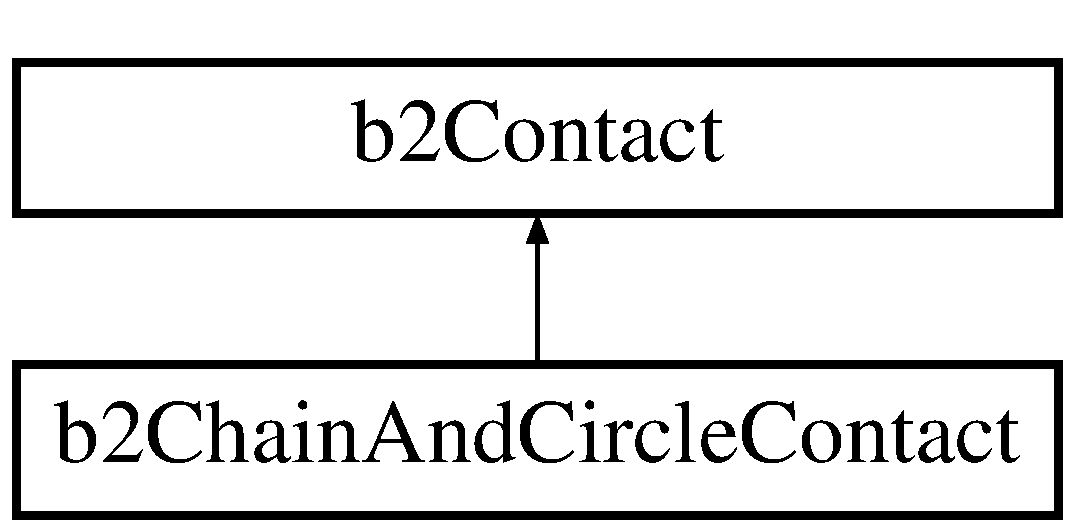
\includegraphics[height=2.000000cm]{classb2ChainAndCircleContact}
\end{center}
\end{figure}
\subsection*{Public Member Functions}
\begin{DoxyCompactItemize}
\item 
\mbox{\Hypertarget{classb2ChainAndCircleContact_a7303997b9af2b859346b4fc4d7e107d5}\label{classb2ChainAndCircleContact_a7303997b9af2b859346b4fc4d7e107d5}} 
{\bfseries b2\+Chain\+And\+Circle\+Contact} (\mbox{\hyperlink{classb2Fixture}{b2\+Fixture}} $\ast$fixtureA, int32 indexA, \mbox{\hyperlink{classb2Fixture}{b2\+Fixture}} $\ast$fixtureB, int32 indexB)
\item 
\mbox{\Hypertarget{classb2ChainAndCircleContact_abdc7f895b76f99f7ddc444ed11986c89}\label{classb2ChainAndCircleContact_abdc7f895b76f99f7ddc444ed11986c89}} 
void \mbox{\hyperlink{classb2ChainAndCircleContact_abdc7f895b76f99f7ddc444ed11986c89}{Evaluate}} (\mbox{\hyperlink{structb2Manifold}{b2\+Manifold}} $\ast$manifold, const \mbox{\hyperlink{structb2Transform}{b2\+Transform}} \&xfA, const \mbox{\hyperlink{structb2Transform}{b2\+Transform}} \&xfB) override
\begin{DoxyCompactList}\small\item\em Evaluate this contact with your own manifold and transforms. \end{DoxyCompactList}\end{DoxyCompactItemize}
\subsection*{Static Public Member Functions}
\begin{DoxyCompactItemize}
\item 
\mbox{\Hypertarget{classb2ChainAndCircleContact_a9738f9b3eeddb824213abaae78ff6a73}\label{classb2ChainAndCircleContact_a9738f9b3eeddb824213abaae78ff6a73}} 
static \mbox{\hyperlink{classb2Contact}{b2\+Contact}} $\ast$ {\bfseries Create} (\mbox{\hyperlink{classb2Fixture}{b2\+Fixture}} $\ast$fixtureA, int32 indexA, \mbox{\hyperlink{classb2Fixture}{b2\+Fixture}} $\ast$fixtureB, int32 indexB, \mbox{\hyperlink{classb2BlockAllocator}{b2\+Block\+Allocator}} $\ast$allocator)
\item 
\mbox{\Hypertarget{classb2ChainAndCircleContact_a1070fc727a3c52a160c7919c9650b4e3}\label{classb2ChainAndCircleContact_a1070fc727a3c52a160c7919c9650b4e3}} 
static void {\bfseries Destroy} (\mbox{\hyperlink{classb2Contact}{b2\+Contact}} $\ast$contact, \mbox{\hyperlink{classb2BlockAllocator}{b2\+Block\+Allocator}} $\ast$allocator)
\end{DoxyCompactItemize}
\subsection*{Additional Inherited Members}


The documentation for this class was generated from the following files\+:\begin{DoxyCompactItemize}
\item 
Dynamics/\+Contacts/b2\+Chain\+And\+Circle\+Contact.\+h\item 
Dynamics/\+Contacts/b2\+Chain\+And\+Circle\+Contact.\+cpp\end{DoxyCompactItemize}

\hypertarget{classb2ChainAndPolygonContact}{}\section{b2\+Chain\+And\+Polygon\+Contact Class Reference}
\label{classb2ChainAndPolygonContact}\index{b2\+Chain\+And\+Polygon\+Contact@{b2\+Chain\+And\+Polygon\+Contact}}
Inheritance diagram for b2\+Chain\+And\+Polygon\+Contact\+:\begin{figure}[H]
\begin{center}
\leavevmode
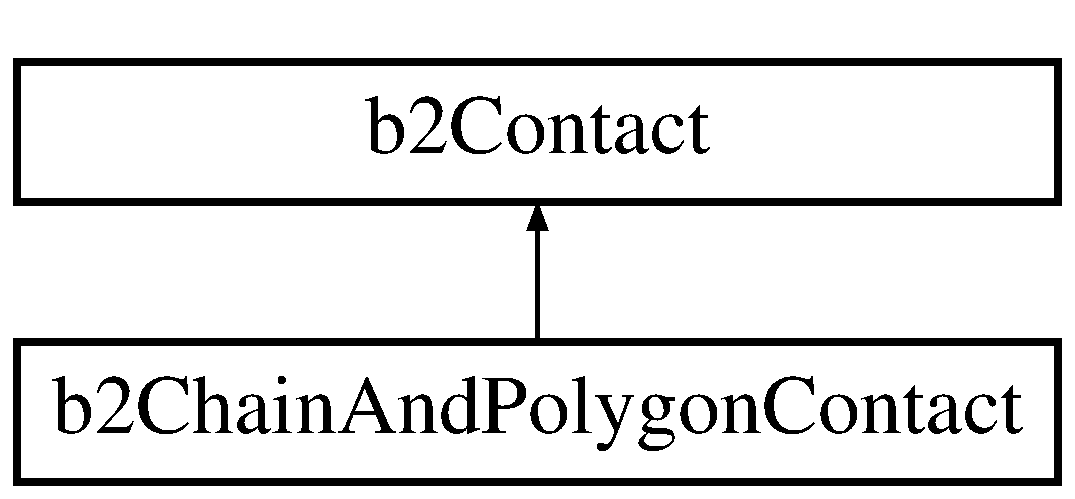
\includegraphics[height=2.000000cm]{classb2ChainAndPolygonContact}
\end{center}
\end{figure}
\subsection*{Public Member Functions}
\begin{DoxyCompactItemize}
\item 
\mbox{\Hypertarget{classb2ChainAndPolygonContact_ae43cd05c72ccaeb5f03efc5df944648b}\label{classb2ChainAndPolygonContact_ae43cd05c72ccaeb5f03efc5df944648b}} 
{\bfseries b2\+Chain\+And\+Polygon\+Contact} (\mbox{\hyperlink{classb2Fixture}{b2\+Fixture}} $\ast$fixtureA, int32 indexA, \mbox{\hyperlink{classb2Fixture}{b2\+Fixture}} $\ast$fixtureB, int32 indexB)
\item 
\mbox{\Hypertarget{classb2ChainAndPolygonContact_a607e7a8b4b0a5ee9bfd100a365fb6f3b}\label{classb2ChainAndPolygonContact_a607e7a8b4b0a5ee9bfd100a365fb6f3b}} 
void \mbox{\hyperlink{classb2ChainAndPolygonContact_a607e7a8b4b0a5ee9bfd100a365fb6f3b}{Evaluate}} (\mbox{\hyperlink{structb2Manifold}{b2\+Manifold}} $\ast$manifold, const \mbox{\hyperlink{structb2Transform}{b2\+Transform}} \&xfA, const \mbox{\hyperlink{structb2Transform}{b2\+Transform}} \&xfB) override
\begin{DoxyCompactList}\small\item\em Evaluate this contact with your own manifold and transforms. \end{DoxyCompactList}\end{DoxyCompactItemize}
\subsection*{Static Public Member Functions}
\begin{DoxyCompactItemize}
\item 
\mbox{\Hypertarget{classb2ChainAndPolygonContact_a03e9021485104ae8f485f986703fcd85}\label{classb2ChainAndPolygonContact_a03e9021485104ae8f485f986703fcd85}} 
static \mbox{\hyperlink{classb2Contact}{b2\+Contact}} $\ast$ {\bfseries Create} (\mbox{\hyperlink{classb2Fixture}{b2\+Fixture}} $\ast$fixtureA, int32 indexA, \mbox{\hyperlink{classb2Fixture}{b2\+Fixture}} $\ast$fixtureB, int32 indexB, \mbox{\hyperlink{classb2BlockAllocator}{b2\+Block\+Allocator}} $\ast$allocator)
\item 
\mbox{\Hypertarget{classb2ChainAndPolygonContact_aa31bf71d64dd78583505b6da76ef289c}\label{classb2ChainAndPolygonContact_aa31bf71d64dd78583505b6da76ef289c}} 
static void {\bfseries Destroy} (\mbox{\hyperlink{classb2Contact}{b2\+Contact}} $\ast$contact, \mbox{\hyperlink{classb2BlockAllocator}{b2\+Block\+Allocator}} $\ast$allocator)
\end{DoxyCompactItemize}
\subsection*{Additional Inherited Members}


The documentation for this class was generated from the following files\+:\begin{DoxyCompactItemize}
\item 
Dynamics/\+Contacts/b2\+Chain\+And\+Polygon\+Contact.\+h\item 
Dynamics/\+Contacts/b2\+Chain\+And\+Polygon\+Contact.\+cpp\end{DoxyCompactItemize}

\hypertarget{classb2ChainShape}{}\section{b2\+Chain\+Shape Class Reference}
\label{classb2ChainShape}\index{b2\+Chain\+Shape@{b2\+Chain\+Shape}}


{\ttfamily \#include $<$b2\+Chain\+Shape.\+h$>$}

Inheritance diagram for b2\+Chain\+Shape\+:\begin{figure}[H]
\begin{center}
\leavevmode
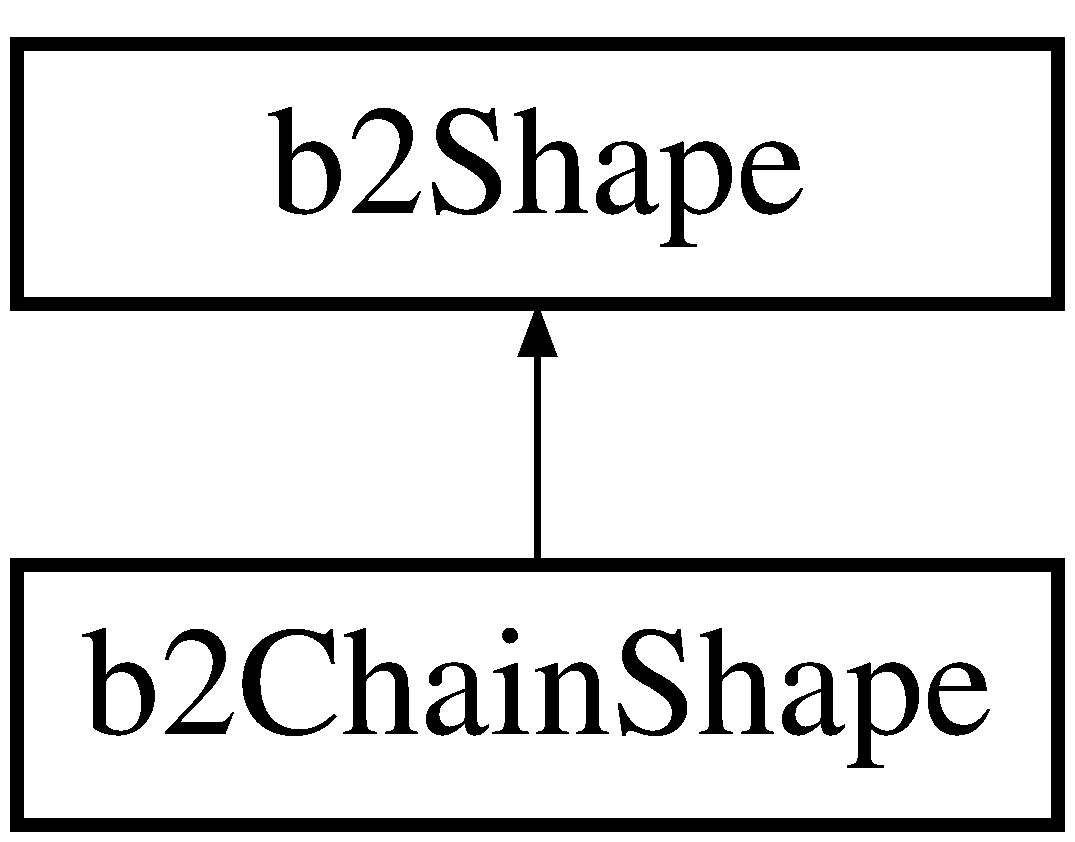
\includegraphics[height=2.000000cm]{classb2ChainShape}
\end{center}
\end{figure}
\subsection*{Public Member Functions}
\begin{DoxyCompactItemize}
\item 
\mbox{\Hypertarget{classb2ChainShape_a8c032394f5a85e7fc425a437e7689a18}\label{classb2ChainShape_a8c032394f5a85e7fc425a437e7689a18}} 
\mbox{\hyperlink{classb2ChainShape_a8c032394f5a85e7fc425a437e7689a18}{$\sim$b2\+Chain\+Shape}} ()
\begin{DoxyCompactList}\small\item\em The destructor frees the vertices using b2\+Free. \end{DoxyCompactList}\item 
\mbox{\Hypertarget{classb2ChainShape_a434d4b61ab15726302ec5ad484011c33}\label{classb2ChainShape_a434d4b61ab15726302ec5ad484011c33}} 
void \mbox{\hyperlink{classb2ChainShape_a434d4b61ab15726302ec5ad484011c33}{Clear}} ()
\begin{DoxyCompactList}\small\item\em Clear all data. \end{DoxyCompactList}\item 
void \mbox{\hyperlink{classb2ChainShape_ac257742a52cac391e25962a4c703fb06}{Create\+Loop}} (const \mbox{\hyperlink{structb2Vec2}{b2\+Vec2}} $\ast$vertices, int32 count)
\item 
void \mbox{\hyperlink{classb2ChainShape_aa0977339b743c05f2179939ccc38e7e0}{Create\+Chain}} (const \mbox{\hyperlink{structb2Vec2}{b2\+Vec2}} $\ast$vertices, int32 count)
\item 
void \mbox{\hyperlink{classb2ChainShape_aeb2ddbe0c52a98885e91b7c8f597315b}{Set\+Prev\+Vertex}} (const \mbox{\hyperlink{structb2Vec2}{b2\+Vec2}} \&prev\+Vertex)
\item 
void \mbox{\hyperlink{classb2ChainShape_a15c7c2821a52266ef57621ac7d34a95f}{Set\+Next\+Vertex}} (const \mbox{\hyperlink{structb2Vec2}{b2\+Vec2}} \&next\+Vertex)
\item 
\mbox{\Hypertarget{classb2ChainShape_a03d2ea80168d29c553fa21b5a821e6d8}\label{classb2ChainShape_a03d2ea80168d29c553fa21b5a821e6d8}} 
\mbox{\hyperlink{classb2Shape}{b2\+Shape}} $\ast$ \mbox{\hyperlink{classb2ChainShape_a03d2ea80168d29c553fa21b5a821e6d8}{Clone}} (\mbox{\hyperlink{classb2BlockAllocator}{b2\+Block\+Allocator}} $\ast$allocator) const override
\begin{DoxyCompactList}\small\item\em Implement \mbox{\hyperlink{classb2Shape}{b2\+Shape}}. Vertices are cloned using b2\+Alloc. \end{DoxyCompactList}\item 
int32 \mbox{\hyperlink{classb2ChainShape_a4d4fd8f5386a30f35b10d1b2848dbe54}{Get\+Child\+Count}} () const override
\item 
\mbox{\Hypertarget{classb2ChainShape_abfe7f836d3c32dc06b920df61a74f412}\label{classb2ChainShape_abfe7f836d3c32dc06b920df61a74f412}} 
void \mbox{\hyperlink{classb2ChainShape_abfe7f836d3c32dc06b920df61a74f412}{Get\+Child\+Edge}} (\mbox{\hyperlink{classb2EdgeShape}{b2\+Edge\+Shape}} $\ast$edge, int32 index) const
\begin{DoxyCompactList}\small\item\em Get a child edge. \end{DoxyCompactList}\item 
bool \mbox{\hyperlink{classb2ChainShape_afd03c8679f18f9962a6c76bde629c62a}{Test\+Point}} (const \mbox{\hyperlink{structb2Transform}{b2\+Transform}} \&transform, const \mbox{\hyperlink{structb2Vec2}{b2\+Vec2}} \&p) const override
\item 
\mbox{\Hypertarget{classb2ChainShape_add9e88f7f90b32ae75738cfb042ef532}\label{classb2ChainShape_add9e88f7f90b32ae75738cfb042ef532}} 
bool \mbox{\hyperlink{classb2ChainShape_add9e88f7f90b32ae75738cfb042ef532}{Ray\+Cast}} (\mbox{\hyperlink{structb2RayCastOutput}{b2\+Ray\+Cast\+Output}} $\ast$output, const \mbox{\hyperlink{structb2RayCastInput}{b2\+Ray\+Cast\+Input}} \&input, const \mbox{\hyperlink{structb2Transform}{b2\+Transform}} \&transform, int32 child\+Index) const override
\begin{DoxyCompactList}\small\item\em Implement \mbox{\hyperlink{classb2Shape}{b2\+Shape}}. \end{DoxyCompactList}\item 
void \mbox{\hyperlink{classb2ChainShape_ae1d7470ce8d32e92d27c149ab45f5468}{Compute\+A\+A\+BB}} (\mbox{\hyperlink{structb2AABB}{b2\+A\+A\+BB}} $\ast$aabb, const \mbox{\hyperlink{structb2Transform}{b2\+Transform}} \&transform, int32 child\+Index) const override
\item 
void \mbox{\hyperlink{classb2ChainShape_aad3671d6eab61f6b26e2f1b6ac50bb98}{Compute\+Mass}} (\mbox{\hyperlink{structb2MassData}{b2\+Mass\+Data}} $\ast$mass\+Data, float32 density) const override
\end{DoxyCompactItemize}
\subsection*{Public Attributes}
\begin{DoxyCompactItemize}
\item 
\mbox{\Hypertarget{classb2ChainShape_a481116a6886fb3880b13e55c966579da}\label{classb2ChainShape_a481116a6886fb3880b13e55c966579da}} 
\mbox{\hyperlink{structb2Vec2}{b2\+Vec2}} $\ast$ \mbox{\hyperlink{classb2ChainShape_a481116a6886fb3880b13e55c966579da}{m\+\_\+vertices}}
\begin{DoxyCompactList}\small\item\em The vertices. Owned by this class. \end{DoxyCompactList}\item 
\mbox{\Hypertarget{classb2ChainShape_ab2ad711781e6ac81179074e90e0e058b}\label{classb2ChainShape_ab2ad711781e6ac81179074e90e0e058b}} 
int32 \mbox{\hyperlink{classb2ChainShape_ab2ad711781e6ac81179074e90e0e058b}{m\+\_\+count}}
\begin{DoxyCompactList}\small\item\em The vertex count. \end{DoxyCompactList}\item 
\mbox{\Hypertarget{classb2ChainShape_a3a42d4c6b2421bc5badda3b6164949cf}\label{classb2ChainShape_a3a42d4c6b2421bc5badda3b6164949cf}} 
\mbox{\hyperlink{structb2Vec2}{b2\+Vec2}} {\bfseries m\+\_\+prev\+Vertex}
\item 
\mbox{\Hypertarget{classb2ChainShape_af3716ef780dd5bcd905e350d8854aaa2}\label{classb2ChainShape_af3716ef780dd5bcd905e350d8854aaa2}} 
\mbox{\hyperlink{structb2Vec2}{b2\+Vec2}} {\bfseries m\+\_\+next\+Vertex}
\item 
\mbox{\Hypertarget{classb2ChainShape_a8a6ffbb9de0e2b8545c8b4fc8aa77249}\label{classb2ChainShape_a8a6ffbb9de0e2b8545c8b4fc8aa77249}} 
bool {\bfseries m\+\_\+has\+Prev\+Vertex}
\item 
\mbox{\Hypertarget{classb2ChainShape_a333b74486566e73c3cf1f7da5e69a96e}\label{classb2ChainShape_a333b74486566e73c3cf1f7da5e69a96e}} 
bool {\bfseries m\+\_\+has\+Next\+Vertex}
\end{DoxyCompactItemize}
\subsection*{Additional Inherited Members}


\subsection{Detailed Description}
A chain shape is a free form sequence of line segments. The chain has two-\/sided collision, so you can use inside and outside collision. Therefore, you may use any winding order. Since there may be many vertices, they are allocated using b2\+Alloc. Connectivity information is used to create smooth collisions. W\+A\+R\+N\+I\+NG\+: The chain will not collide properly if there are self-\/intersections. 

\subsection{Member Function Documentation}
\mbox{\Hypertarget{classb2ChainShape_ae1d7470ce8d32e92d27c149ab45f5468}\label{classb2ChainShape_ae1d7470ce8d32e92d27c149ab45f5468}} 
\index{b2\+Chain\+Shape@{b2\+Chain\+Shape}!Compute\+A\+A\+BB@{Compute\+A\+A\+BB}}
\index{Compute\+A\+A\+BB@{Compute\+A\+A\+BB}!b2\+Chain\+Shape@{b2\+Chain\+Shape}}
\subsubsection{\texorpdfstring{Compute\+A\+A\+B\+B()}{ComputeAABB()}}
{\footnotesize\ttfamily void b2\+Chain\+Shape\+::\+Compute\+A\+A\+BB (\begin{DoxyParamCaption}\item[{\mbox{\hyperlink{structb2AABB}{b2\+A\+A\+BB}} $\ast$}]{aabb,  }\item[{const \mbox{\hyperlink{structb2Transform}{b2\+Transform}} \&}]{transform,  }\item[{int32}]{child\+Index }\end{DoxyParamCaption}) const\hspace{0.3cm}{\ttfamily [override]}, {\ttfamily [virtual]}}

\begin{DoxySeeAlso}{See also}
\mbox{\hyperlink{classb2Shape_a88e9807fab0c8ca9a98d8926e50a1411}{b2\+Shape\+::\+Compute\+A\+A\+BB}} 
\end{DoxySeeAlso}


Implements \mbox{\hyperlink{classb2Shape_a88e9807fab0c8ca9a98d8926e50a1411}{b2\+Shape}}.

\mbox{\Hypertarget{classb2ChainShape_aad3671d6eab61f6b26e2f1b6ac50bb98}\label{classb2ChainShape_aad3671d6eab61f6b26e2f1b6ac50bb98}} 
\index{b2\+Chain\+Shape@{b2\+Chain\+Shape}!Compute\+Mass@{Compute\+Mass}}
\index{Compute\+Mass@{Compute\+Mass}!b2\+Chain\+Shape@{b2\+Chain\+Shape}}
\subsubsection{\texorpdfstring{Compute\+Mass()}{ComputeMass()}}
{\footnotesize\ttfamily void b2\+Chain\+Shape\+::\+Compute\+Mass (\begin{DoxyParamCaption}\item[{\mbox{\hyperlink{structb2MassData}{b2\+Mass\+Data}} $\ast$}]{mass\+Data,  }\item[{float32}]{density }\end{DoxyParamCaption}) const\hspace{0.3cm}{\ttfamily [override]}, {\ttfamily [virtual]}}

Chains have zero mass. \begin{DoxySeeAlso}{See also}
\mbox{\hyperlink{classb2Shape_a61b365526241b47f124789b0309cac69}{b2\+Shape\+::\+Compute\+Mass}} 
\end{DoxySeeAlso}


Implements \mbox{\hyperlink{classb2Shape_a61b365526241b47f124789b0309cac69}{b2\+Shape}}.

\mbox{\Hypertarget{classb2ChainShape_aa0977339b743c05f2179939ccc38e7e0}\label{classb2ChainShape_aa0977339b743c05f2179939ccc38e7e0}} 
\index{b2\+Chain\+Shape@{b2\+Chain\+Shape}!Create\+Chain@{Create\+Chain}}
\index{Create\+Chain@{Create\+Chain}!b2\+Chain\+Shape@{b2\+Chain\+Shape}}
\subsubsection{\texorpdfstring{Create\+Chain()}{CreateChain()}}
{\footnotesize\ttfamily void b2\+Chain\+Shape\+::\+Create\+Chain (\begin{DoxyParamCaption}\item[{const \mbox{\hyperlink{structb2Vec2}{b2\+Vec2}} $\ast$}]{vertices,  }\item[{int32}]{count }\end{DoxyParamCaption})}

Create a chain with isolated end vertices. 
\begin{DoxyParams}{Parameters}
{\em vertices} & an array of vertices, these are copied \\
\hline
{\em count} & the vertex count \\
\hline
\end{DoxyParams}
\mbox{\Hypertarget{classb2ChainShape_ac257742a52cac391e25962a4c703fb06}\label{classb2ChainShape_ac257742a52cac391e25962a4c703fb06}} 
\index{b2\+Chain\+Shape@{b2\+Chain\+Shape}!Create\+Loop@{Create\+Loop}}
\index{Create\+Loop@{Create\+Loop}!b2\+Chain\+Shape@{b2\+Chain\+Shape}}
\subsubsection{\texorpdfstring{Create\+Loop()}{CreateLoop()}}
{\footnotesize\ttfamily void b2\+Chain\+Shape\+::\+Create\+Loop (\begin{DoxyParamCaption}\item[{const \mbox{\hyperlink{structb2Vec2}{b2\+Vec2}} $\ast$}]{vertices,  }\item[{int32}]{count }\end{DoxyParamCaption})}

Create a loop. This automatically adjusts connectivity. 
\begin{DoxyParams}{Parameters}
{\em vertices} & an array of vertices, these are copied \\
\hline
{\em count} & the vertex count \\
\hline
\end{DoxyParams}
\mbox{\Hypertarget{classb2ChainShape_a4d4fd8f5386a30f35b10d1b2848dbe54}\label{classb2ChainShape_a4d4fd8f5386a30f35b10d1b2848dbe54}} 
\index{b2\+Chain\+Shape@{b2\+Chain\+Shape}!Get\+Child\+Count@{Get\+Child\+Count}}
\index{Get\+Child\+Count@{Get\+Child\+Count}!b2\+Chain\+Shape@{b2\+Chain\+Shape}}
\subsubsection{\texorpdfstring{Get\+Child\+Count()}{GetChildCount()}}
{\footnotesize\ttfamily int32 b2\+Chain\+Shape\+::\+Get\+Child\+Count (\begin{DoxyParamCaption}{ }\end{DoxyParamCaption}) const\hspace{0.3cm}{\ttfamily [override]}, {\ttfamily [virtual]}}

\begin{DoxySeeAlso}{See also}
\mbox{\hyperlink{classb2Shape_a05a3c445017d96df9238ceefe6ce37ab}{b2\+Shape\+::\+Get\+Child\+Count}} 
\end{DoxySeeAlso}


Implements \mbox{\hyperlink{classb2Shape_a05a3c445017d96df9238ceefe6ce37ab}{b2\+Shape}}.

\mbox{\Hypertarget{classb2ChainShape_a15c7c2821a52266ef57621ac7d34a95f}\label{classb2ChainShape_a15c7c2821a52266ef57621ac7d34a95f}} 
\index{b2\+Chain\+Shape@{b2\+Chain\+Shape}!Set\+Next\+Vertex@{Set\+Next\+Vertex}}
\index{Set\+Next\+Vertex@{Set\+Next\+Vertex}!b2\+Chain\+Shape@{b2\+Chain\+Shape}}
\subsubsection{\texorpdfstring{Set\+Next\+Vertex()}{SetNextVertex()}}
{\footnotesize\ttfamily void b2\+Chain\+Shape\+::\+Set\+Next\+Vertex (\begin{DoxyParamCaption}\item[{const \mbox{\hyperlink{structb2Vec2}{b2\+Vec2}} \&}]{next\+Vertex }\end{DoxyParamCaption})}

Establish connectivity to a vertex that follows the last vertex. Don\textquotesingle{}t call this for loops. \mbox{\Hypertarget{classb2ChainShape_aeb2ddbe0c52a98885e91b7c8f597315b}\label{classb2ChainShape_aeb2ddbe0c52a98885e91b7c8f597315b}} 
\index{b2\+Chain\+Shape@{b2\+Chain\+Shape}!Set\+Prev\+Vertex@{Set\+Prev\+Vertex}}
\index{Set\+Prev\+Vertex@{Set\+Prev\+Vertex}!b2\+Chain\+Shape@{b2\+Chain\+Shape}}
\subsubsection{\texorpdfstring{Set\+Prev\+Vertex()}{SetPrevVertex()}}
{\footnotesize\ttfamily void b2\+Chain\+Shape\+::\+Set\+Prev\+Vertex (\begin{DoxyParamCaption}\item[{const \mbox{\hyperlink{structb2Vec2}{b2\+Vec2}} \&}]{prev\+Vertex }\end{DoxyParamCaption})}

Establish connectivity to a vertex that precedes the first vertex. Don\textquotesingle{}t call this for loops. \mbox{\Hypertarget{classb2ChainShape_afd03c8679f18f9962a6c76bde629c62a}\label{classb2ChainShape_afd03c8679f18f9962a6c76bde629c62a}} 
\index{b2\+Chain\+Shape@{b2\+Chain\+Shape}!Test\+Point@{Test\+Point}}
\index{Test\+Point@{Test\+Point}!b2\+Chain\+Shape@{b2\+Chain\+Shape}}
\subsubsection{\texorpdfstring{Test\+Point()}{TestPoint()}}
{\footnotesize\ttfamily bool b2\+Chain\+Shape\+::\+Test\+Point (\begin{DoxyParamCaption}\item[{const \mbox{\hyperlink{structb2Transform}{b2\+Transform}} \&}]{transform,  }\item[{const \mbox{\hyperlink{structb2Vec2}{b2\+Vec2}} \&}]{p }\end{DoxyParamCaption}) const\hspace{0.3cm}{\ttfamily [override]}, {\ttfamily [virtual]}}

This always return false. \begin{DoxySeeAlso}{See also}
\mbox{\hyperlink{classb2Shape_a6ac968e403e2d93e8ae46d728a2e50fa}{b2\+Shape\+::\+Test\+Point}} 
\end{DoxySeeAlso}


Implements \mbox{\hyperlink{classb2Shape_a6ac968e403e2d93e8ae46d728a2e50fa}{b2\+Shape}}.



The documentation for this class was generated from the following files\+:\begin{DoxyCompactItemize}
\item 
Collision/\+Shapes/b2\+Chain\+Shape.\+h\item 
Collision/\+Shapes/b2\+Chain\+Shape.\+cpp\end{DoxyCompactItemize}

\hypertarget{structb2Chunk}{}\section{b2\+Chunk Struct Reference}
\label{structb2Chunk}\index{b2\+Chunk@{b2\+Chunk}}
\subsection*{Public Attributes}
\begin{DoxyCompactItemize}
\item 
\mbox{\Hypertarget{structb2Chunk_a731df6d026298426622990c251cf742a}\label{structb2Chunk_a731df6d026298426622990c251cf742a}} 
int32 {\bfseries block\+Size}
\item 
\mbox{\Hypertarget{structb2Chunk_aa45617a36287b3dea2130c426cfd42d2}\label{structb2Chunk_aa45617a36287b3dea2130c426cfd42d2}} 
\mbox{\hyperlink{structb2Block}{b2\+Block}} $\ast$ {\bfseries blocks}
\end{DoxyCompactItemize}


The documentation for this struct was generated from the following file\+:\begin{DoxyCompactItemize}
\item 
Common/b2\+Block\+Allocator.\+cpp\end{DoxyCompactItemize}

\hypertarget{classb2CircleContact}{}\section{b2\+Circle\+Contact Class Reference}
\label{classb2CircleContact}\index{b2\+Circle\+Contact@{b2\+Circle\+Contact}}
Inheritance diagram for b2\+Circle\+Contact\+:\begin{figure}[H]
\begin{center}
\leavevmode
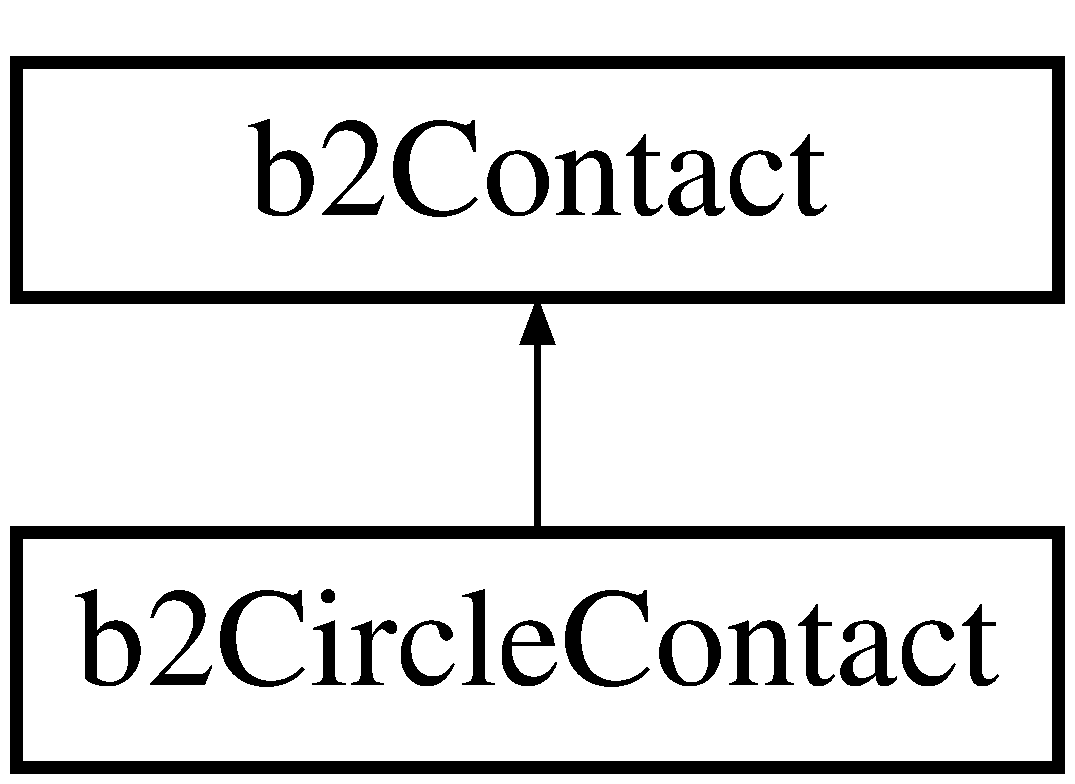
\includegraphics[height=2.000000cm]{classb2CircleContact}
\end{center}
\end{figure}
\subsection*{Public Member Functions}
\begin{DoxyCompactItemize}
\item 
\mbox{\Hypertarget{classb2CircleContact_a77e06c857edb2ca171340898f09ef789}\label{classb2CircleContact_a77e06c857edb2ca171340898f09ef789}} 
{\bfseries b2\+Circle\+Contact} (\mbox{\hyperlink{classb2Fixture}{b2\+Fixture}} $\ast$fixtureA, \mbox{\hyperlink{classb2Fixture}{b2\+Fixture}} $\ast$fixtureB)
\item 
\mbox{\Hypertarget{classb2CircleContact_a90036965fd66469e916a5afc6c244092}\label{classb2CircleContact_a90036965fd66469e916a5afc6c244092}} 
void \mbox{\hyperlink{classb2CircleContact_a90036965fd66469e916a5afc6c244092}{Evaluate}} (\mbox{\hyperlink{structb2Manifold}{b2\+Manifold}} $\ast$manifold, const \mbox{\hyperlink{structb2Transform}{b2\+Transform}} \&xfA, const \mbox{\hyperlink{structb2Transform}{b2\+Transform}} \&xfB) override
\begin{DoxyCompactList}\small\item\em Evaluate this contact with your own manifold and transforms. \end{DoxyCompactList}\end{DoxyCompactItemize}
\subsection*{Static Public Member Functions}
\begin{DoxyCompactItemize}
\item 
\mbox{\Hypertarget{classb2CircleContact_ab0ea452487cb19217ae8480dbc22fd41}\label{classb2CircleContact_ab0ea452487cb19217ae8480dbc22fd41}} 
static \mbox{\hyperlink{classb2Contact}{b2\+Contact}} $\ast$ {\bfseries Create} (\mbox{\hyperlink{classb2Fixture}{b2\+Fixture}} $\ast$fixtureA, int32 indexA, \mbox{\hyperlink{classb2Fixture}{b2\+Fixture}} $\ast$fixtureB, int32 indexB, \mbox{\hyperlink{classb2BlockAllocator}{b2\+Block\+Allocator}} $\ast$allocator)
\item 
\mbox{\Hypertarget{classb2CircleContact_a4ca67c653a18d88180e49149f0df742a}\label{classb2CircleContact_a4ca67c653a18d88180e49149f0df742a}} 
static void {\bfseries Destroy} (\mbox{\hyperlink{classb2Contact}{b2\+Contact}} $\ast$contact, \mbox{\hyperlink{classb2BlockAllocator}{b2\+Block\+Allocator}} $\ast$allocator)
\end{DoxyCompactItemize}
\subsection*{Additional Inherited Members}


The documentation for this class was generated from the following files\+:\begin{DoxyCompactItemize}
\item 
Dynamics/\+Contacts/b2\+Circle\+Contact.\+h\item 
Dynamics/\+Contacts/b2\+Circle\+Contact.\+cpp\end{DoxyCompactItemize}

\hypertarget{classb2CircleShape}{}\section{b2\+Circle\+Shape Class Reference}
\label{classb2CircleShape}\index{b2\+Circle\+Shape@{b2\+Circle\+Shape}}


A circle shape.  




{\ttfamily \#include $<$b2\+Circle\+Shape.\+h$>$}

Inheritance diagram for b2\+Circle\+Shape\+:\begin{figure}[H]
\begin{center}
\leavevmode
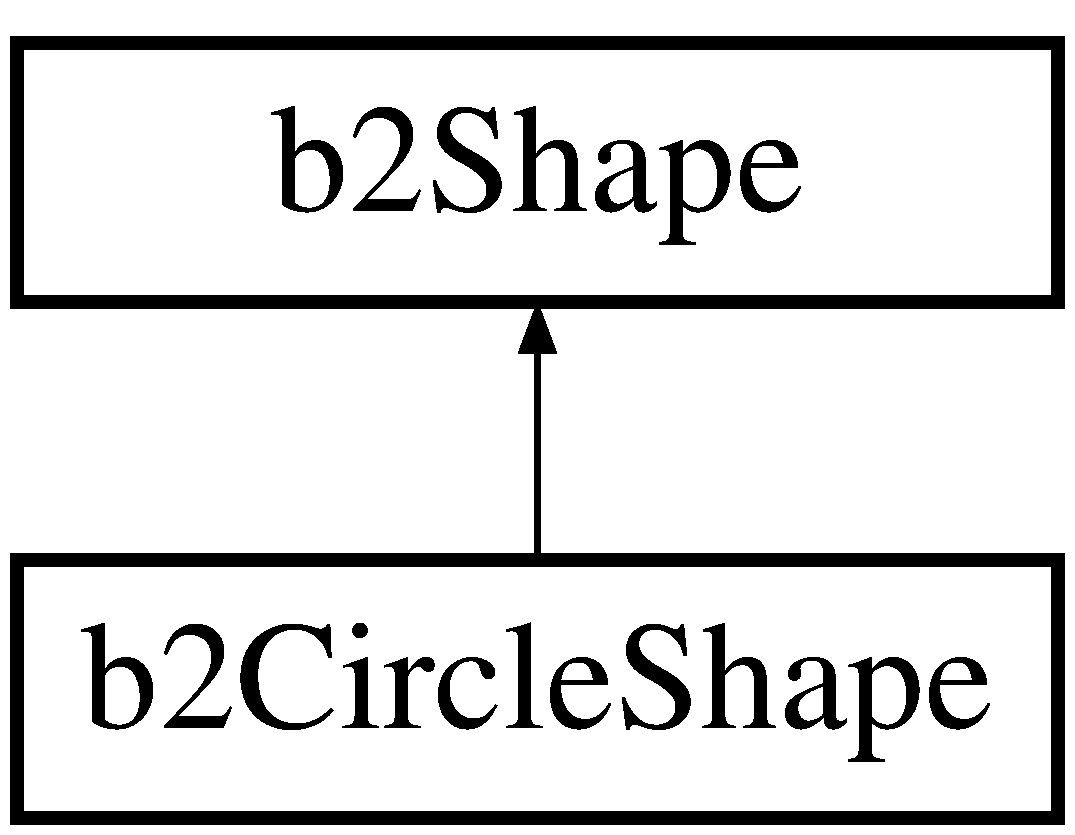
\includegraphics[height=2.000000cm]{classb2CircleShape}
\end{center}
\end{figure}
\subsection*{Public Member Functions}
\begin{DoxyCompactItemize}
\item 
\mbox{\Hypertarget{classb2CircleShape_a5ff8fbab7dff87784fbff20b07e55cfc}\label{classb2CircleShape_a5ff8fbab7dff87784fbff20b07e55cfc}} 
\mbox{\hyperlink{classb2Shape}{b2\+Shape}} $\ast$ \mbox{\hyperlink{classb2CircleShape_a5ff8fbab7dff87784fbff20b07e55cfc}{Clone}} (\mbox{\hyperlink{classb2BlockAllocator}{b2\+Block\+Allocator}} $\ast$allocator) const override
\begin{DoxyCompactList}\small\item\em Implement \mbox{\hyperlink{classb2Shape}{b2\+Shape}}. \end{DoxyCompactList}\item 
int32 \mbox{\hyperlink{classb2CircleShape_a552db3402aed5d12c3177981e5208065}{Get\+Child\+Count}} () const override
\item 
\mbox{\Hypertarget{classb2CircleShape_a84e22b3807e84b72f2981010fc197099}\label{classb2CircleShape_a84e22b3807e84b72f2981010fc197099}} 
bool \mbox{\hyperlink{classb2CircleShape_a84e22b3807e84b72f2981010fc197099}{Test\+Point}} (const \mbox{\hyperlink{structb2Transform}{b2\+Transform}} \&transform, const \mbox{\hyperlink{structb2Vec2}{b2\+Vec2}} \&p) const override
\begin{DoxyCompactList}\small\item\em Implement \mbox{\hyperlink{classb2Shape}{b2\+Shape}}. \end{DoxyCompactList}\item 
\mbox{\Hypertarget{classb2CircleShape_a442e847b9fc3d1344b02b48d490eb0c6}\label{classb2CircleShape_a442e847b9fc3d1344b02b48d490eb0c6}} 
bool \mbox{\hyperlink{classb2CircleShape_a442e847b9fc3d1344b02b48d490eb0c6}{Ray\+Cast}} (\mbox{\hyperlink{structb2RayCastOutput}{b2\+Ray\+Cast\+Output}} $\ast$output, const \mbox{\hyperlink{structb2RayCastInput}{b2\+Ray\+Cast\+Input}} \&input, const \mbox{\hyperlink{structb2Transform}{b2\+Transform}} \&transform, int32 child\+Index) const override
\begin{DoxyCompactList}\small\item\em Implement \mbox{\hyperlink{classb2Shape}{b2\+Shape}}. \end{DoxyCompactList}\item 
void \mbox{\hyperlink{classb2CircleShape_af4a4ea78780af7a7ce40bf5d54affe83}{Compute\+A\+A\+BB}} (\mbox{\hyperlink{structb2AABB}{b2\+A\+A\+BB}} $\ast$aabb, const \mbox{\hyperlink{structb2Transform}{b2\+Transform}} \&transform, int32 child\+Index) const override
\item 
void \mbox{\hyperlink{classb2CircleShape_a7dc07891abd015863fbf03076e47eec5}{Compute\+Mass}} (\mbox{\hyperlink{structb2MassData}{b2\+Mass\+Data}} $\ast$mass\+Data, float32 density) const override
\end{DoxyCompactItemize}
\subsection*{Public Attributes}
\begin{DoxyCompactItemize}
\item 
\mbox{\Hypertarget{classb2CircleShape_a190705618b2e65f636f1dc03c63640ff}\label{classb2CircleShape_a190705618b2e65f636f1dc03c63640ff}} 
\mbox{\hyperlink{structb2Vec2}{b2\+Vec2}} \mbox{\hyperlink{classb2CircleShape_a190705618b2e65f636f1dc03c63640ff}{m\+\_\+p}}
\begin{DoxyCompactList}\small\item\em Position. \end{DoxyCompactList}\end{DoxyCompactItemize}
\subsection*{Additional Inherited Members}


\subsection{Detailed Description}
A circle shape. 

\subsection{Member Function Documentation}
\mbox{\Hypertarget{classb2CircleShape_af4a4ea78780af7a7ce40bf5d54affe83}\label{classb2CircleShape_af4a4ea78780af7a7ce40bf5d54affe83}} 
\index{b2\+Circle\+Shape@{b2\+Circle\+Shape}!Compute\+A\+A\+BB@{Compute\+A\+A\+BB}}
\index{Compute\+A\+A\+BB@{Compute\+A\+A\+BB}!b2\+Circle\+Shape@{b2\+Circle\+Shape}}
\subsubsection{\texorpdfstring{Compute\+A\+A\+B\+B()}{ComputeAABB()}}
{\footnotesize\ttfamily void b2\+Circle\+Shape\+::\+Compute\+A\+A\+BB (\begin{DoxyParamCaption}\item[{\mbox{\hyperlink{structb2AABB}{b2\+A\+A\+BB}} $\ast$}]{aabb,  }\item[{const \mbox{\hyperlink{structb2Transform}{b2\+Transform}} \&}]{transform,  }\item[{int32}]{child\+Index }\end{DoxyParamCaption}) const\hspace{0.3cm}{\ttfamily [override]}, {\ttfamily [virtual]}}

\begin{DoxySeeAlso}{See also}
\mbox{\hyperlink{classb2Shape_a88e9807fab0c8ca9a98d8926e50a1411}{b2\+Shape\+::\+Compute\+A\+A\+BB}} 
\end{DoxySeeAlso}


Implements \mbox{\hyperlink{classb2Shape_a88e9807fab0c8ca9a98d8926e50a1411}{b2\+Shape}}.

\mbox{\Hypertarget{classb2CircleShape_a7dc07891abd015863fbf03076e47eec5}\label{classb2CircleShape_a7dc07891abd015863fbf03076e47eec5}} 
\index{b2\+Circle\+Shape@{b2\+Circle\+Shape}!Compute\+Mass@{Compute\+Mass}}
\index{Compute\+Mass@{Compute\+Mass}!b2\+Circle\+Shape@{b2\+Circle\+Shape}}
\subsubsection{\texorpdfstring{Compute\+Mass()}{ComputeMass()}}
{\footnotesize\ttfamily void b2\+Circle\+Shape\+::\+Compute\+Mass (\begin{DoxyParamCaption}\item[{\mbox{\hyperlink{structb2MassData}{b2\+Mass\+Data}} $\ast$}]{mass\+Data,  }\item[{float32}]{density }\end{DoxyParamCaption}) const\hspace{0.3cm}{\ttfamily [override]}, {\ttfamily [virtual]}}

\begin{DoxySeeAlso}{See also}
\mbox{\hyperlink{classb2Shape_a61b365526241b47f124789b0309cac69}{b2\+Shape\+::\+Compute\+Mass}} 
\end{DoxySeeAlso}


Implements \mbox{\hyperlink{classb2Shape_a61b365526241b47f124789b0309cac69}{b2\+Shape}}.

\mbox{\Hypertarget{classb2CircleShape_a552db3402aed5d12c3177981e5208065}\label{classb2CircleShape_a552db3402aed5d12c3177981e5208065}} 
\index{b2\+Circle\+Shape@{b2\+Circle\+Shape}!Get\+Child\+Count@{Get\+Child\+Count}}
\index{Get\+Child\+Count@{Get\+Child\+Count}!b2\+Circle\+Shape@{b2\+Circle\+Shape}}
\subsubsection{\texorpdfstring{Get\+Child\+Count()}{GetChildCount()}}
{\footnotesize\ttfamily int32 b2\+Circle\+Shape\+::\+Get\+Child\+Count (\begin{DoxyParamCaption}{ }\end{DoxyParamCaption}) const\hspace{0.3cm}{\ttfamily [override]}, {\ttfamily [virtual]}}

\begin{DoxySeeAlso}{See also}
\mbox{\hyperlink{classb2Shape_a05a3c445017d96df9238ceefe6ce37ab}{b2\+Shape\+::\+Get\+Child\+Count}} 
\end{DoxySeeAlso}


Implements \mbox{\hyperlink{classb2Shape_a05a3c445017d96df9238ceefe6ce37ab}{b2\+Shape}}.



The documentation for this class was generated from the following files\+:\begin{DoxyCompactItemize}
\item 
Collision/\+Shapes/b2\+Circle\+Shape.\+h\item 
Collision/\+Shapes/b2\+Circle\+Shape.\+cpp\end{DoxyCompactItemize}

\hypertarget{structb2ClipVertex}{}\section{b2\+Clip\+Vertex Struct Reference}
\label{structb2ClipVertex}\index{b2\+Clip\+Vertex@{b2\+Clip\+Vertex}}


Used for computing contact manifolds.  




{\ttfamily \#include $<$b2\+Collision.\+h$>$}

\subsection*{Public Attributes}
\begin{DoxyCompactItemize}
\item 
\mbox{\Hypertarget{structb2ClipVertex_a6c8d8e4c0667755d5295a9c0d91d5b87}\label{structb2ClipVertex_a6c8d8e4c0667755d5295a9c0d91d5b87}} 
\mbox{\hyperlink{structb2Vec2}{b2\+Vec2}} {\bfseries v}
\item 
\mbox{\Hypertarget{structb2ClipVertex_ac0f6d48eafc40a665bc18d4aa821689d}\label{structb2ClipVertex_ac0f6d48eafc40a665bc18d4aa821689d}} 
\mbox{\hyperlink{unionb2ContactID}{b2\+Contact\+ID}} {\bfseries id}
\end{DoxyCompactItemize}


\subsection{Detailed Description}
Used for computing contact manifolds. 

The documentation for this struct was generated from the following file\+:\begin{DoxyCompactItemize}
\item 
Collision/\mbox{\hyperlink{b2Collision_8h}{b2\+Collision.\+h}}\end{DoxyCompactItemize}

\hypertarget{structb2Color}{}\section{b2\+Color Struct Reference}
\label{structb2Color}\index{b2\+Color@{b2\+Color}}


Color for debug drawing. Each value has the range \mbox{[}0,1\mbox{]}.  




{\ttfamily \#include $<$b2\+Draw.\+h$>$}

\subsection*{Public Member Functions}
\begin{DoxyCompactItemize}
\item 
\mbox{\Hypertarget{structb2Color_a7cceec6dae0dccd757f35eacd41595c6}\label{structb2Color_a7cceec6dae0dccd757f35eacd41595c6}} 
{\bfseries b2\+Color} (float32 r\+In, float32 g\+In, float32 b\+In, float32 a\+In=1.\+0f)
\item 
\mbox{\Hypertarget{structb2Color_aecd71c7fe34182071a5e4699c4fd5cae}\label{structb2Color_aecd71c7fe34182071a5e4699c4fd5cae}} 
void {\bfseries Set} (float32 r\+In, float32 g\+In, float32 b\+In, float32 a\+In=1.\+0f)
\end{DoxyCompactItemize}
\subsection*{Public Attributes}
\begin{DoxyCompactItemize}
\item 
\mbox{\Hypertarget{structb2Color_a9ab6c9a910caee177d96980b74ffb00b}\label{structb2Color_a9ab6c9a910caee177d96980b74ffb00b}} 
float32 {\bfseries r}
\item 
\mbox{\Hypertarget{structb2Color_a241c742352403ec456b51ac5f2abe7d9}\label{structb2Color_a241c742352403ec456b51ac5f2abe7d9}} 
float32 {\bfseries g}
\item 
\mbox{\Hypertarget{structb2Color_a9e7380d27a63010cfad49b97f66dcd26}\label{structb2Color_a9e7380d27a63010cfad49b97f66dcd26}} 
float32 {\bfseries b}
\item 
\mbox{\Hypertarget{structb2Color_adf752d6bc4b05221be1d964e47cf716d}\label{structb2Color_adf752d6bc4b05221be1d964e47cf716d}} 
float32 {\bfseries a}
\end{DoxyCompactItemize}


\subsection{Detailed Description}
Color for debug drawing. Each value has the range \mbox{[}0,1\mbox{]}. 

The documentation for this struct was generated from the following file\+:\begin{DoxyCompactItemize}
\item 
Common/b2\+Draw.\+h\end{DoxyCompactItemize}

\hypertarget{classb2Contact}{}\section{b2\+Contact Class Reference}
\label{classb2Contact}\index{b2\+Contact@{b2\+Contact}}


{\ttfamily \#include $<$b2\+Contact.\+h$>$}

Inheritance diagram for b2\+Contact\+:\begin{figure}[H]
\begin{center}
\leavevmode
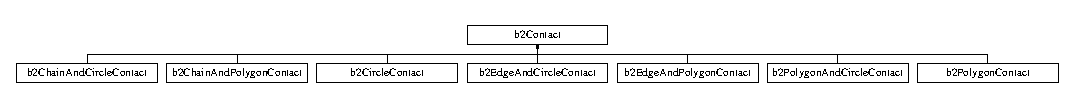
\includegraphics[height=0.888889cm]{classb2Contact}
\end{center}
\end{figure}
\subsection*{Public Member Functions}
\begin{DoxyCompactItemize}
\item 
\mbox{\hyperlink{structb2Manifold}{b2\+Manifold}} $\ast$ \mbox{\hyperlink{classb2Contact_ab0597077b23615476327f9b32d9c4979}{Get\+Manifold}} ()
\item 
\mbox{\Hypertarget{classb2Contact_a4a0a4ee449a4a6fbb8c39567fa10bc2b}\label{classb2Contact_a4a0a4ee449a4a6fbb8c39567fa10bc2b}} 
const \mbox{\hyperlink{structb2Manifold}{b2\+Manifold}} $\ast$ {\bfseries Get\+Manifold} () const
\item 
\mbox{\Hypertarget{classb2Contact_a7f5645863f6197fa28cc1baafbd11255}\label{classb2Contact_a7f5645863f6197fa28cc1baafbd11255}} 
void \mbox{\hyperlink{classb2Contact_a7f5645863f6197fa28cc1baafbd11255}{Get\+World\+Manifold}} (\mbox{\hyperlink{structb2WorldManifold}{b2\+World\+Manifold}} $\ast$world\+Manifold) const
\begin{DoxyCompactList}\small\item\em Get the world manifold. \end{DoxyCompactList}\item 
\mbox{\Hypertarget{classb2Contact_a681346f93e2a27403383775a752c06a0}\label{classb2Contact_a681346f93e2a27403383775a752c06a0}} 
bool \mbox{\hyperlink{classb2Contact_a681346f93e2a27403383775a752c06a0}{Is\+Touching}} () const
\begin{DoxyCompactList}\small\item\em Is this contact touching? \end{DoxyCompactList}\item 
void \mbox{\hyperlink{classb2Contact_a6edf582f8c161d6632854cddefe55a0c}{Set\+Enabled}} (bool flag)
\item 
\mbox{\Hypertarget{classb2Contact_af81964f40dce556efbc83ae760f166b0}\label{classb2Contact_af81964f40dce556efbc83ae760f166b0}} 
bool \mbox{\hyperlink{classb2Contact_af81964f40dce556efbc83ae760f166b0}{Is\+Enabled}} () const
\begin{DoxyCompactList}\small\item\em Has this contact been disabled? \end{DoxyCompactList}\item 
\mbox{\Hypertarget{classb2Contact_aebfebb1e4b27dc0bd7aa120093e3d650}\label{classb2Contact_aebfebb1e4b27dc0bd7aa120093e3d650}} 
\mbox{\hyperlink{classb2Contact}{b2\+Contact}} $\ast$ \mbox{\hyperlink{classb2Contact_aebfebb1e4b27dc0bd7aa120093e3d650}{Get\+Next}} ()
\begin{DoxyCompactList}\small\item\em Get the next contact in the world\textquotesingle{}s contact list. \end{DoxyCompactList}\item 
\mbox{\Hypertarget{classb2Contact_a5231c6fe1b2b374ac9909a248aee0c98}\label{classb2Contact_a5231c6fe1b2b374ac9909a248aee0c98}} 
const \mbox{\hyperlink{classb2Contact}{b2\+Contact}} $\ast$ {\bfseries Get\+Next} () const
\item 
\mbox{\Hypertarget{classb2Contact_a707a3a5a14c2cdd4c6eb7fc648d76037}\label{classb2Contact_a707a3a5a14c2cdd4c6eb7fc648d76037}} 
\mbox{\hyperlink{classb2Fixture}{b2\+Fixture}} $\ast$ \mbox{\hyperlink{classb2Contact_a707a3a5a14c2cdd4c6eb7fc648d76037}{Get\+FixtureA}} ()
\begin{DoxyCompactList}\small\item\em Get fixture A in this contact. \end{DoxyCompactList}\item 
\mbox{\Hypertarget{classb2Contact_ad3c9e8c69128efbe03af632c1acc7776}\label{classb2Contact_ad3c9e8c69128efbe03af632c1acc7776}} 
const \mbox{\hyperlink{classb2Fixture}{b2\+Fixture}} $\ast$ {\bfseries Get\+FixtureA} () const
\item 
\mbox{\Hypertarget{classb2Contact_aa0b0739e6615ba8d38e9b5bd8761dc31}\label{classb2Contact_aa0b0739e6615ba8d38e9b5bd8761dc31}} 
int32 \mbox{\hyperlink{classb2Contact_aa0b0739e6615ba8d38e9b5bd8761dc31}{Get\+Child\+IndexA}} () const
\begin{DoxyCompactList}\small\item\em Get the child primitive index for fixture A. \end{DoxyCompactList}\item 
\mbox{\Hypertarget{classb2Contact_a68464fe587d7e6a1f52763e965bb7361}\label{classb2Contact_a68464fe587d7e6a1f52763e965bb7361}} 
\mbox{\hyperlink{classb2Fixture}{b2\+Fixture}} $\ast$ \mbox{\hyperlink{classb2Contact_a68464fe587d7e6a1f52763e965bb7361}{Get\+FixtureB}} ()
\begin{DoxyCompactList}\small\item\em Get fixture B in this contact. \end{DoxyCompactList}\item 
\mbox{\Hypertarget{classb2Contact_aa89780a20a2b7cd424c09adca9917546}\label{classb2Contact_aa89780a20a2b7cd424c09adca9917546}} 
const \mbox{\hyperlink{classb2Fixture}{b2\+Fixture}} $\ast$ {\bfseries Get\+FixtureB} () const
\item 
\mbox{\Hypertarget{classb2Contact_aab201068e7f2cc31c69b1f5c8471d672}\label{classb2Contact_aab201068e7f2cc31c69b1f5c8471d672}} 
int32 \mbox{\hyperlink{classb2Contact_aab201068e7f2cc31c69b1f5c8471d672}{Get\+Child\+IndexB}} () const
\begin{DoxyCompactList}\small\item\em Get the child primitive index for fixture B. \end{DoxyCompactList}\item 
void \mbox{\hyperlink{classb2Contact_a5e8fbb6bb2966ac84272bb0ea9d2e4c7}{Set\+Friction}} (float32 friction)
\item 
\mbox{\Hypertarget{classb2Contact_a7650ec27931c82f3914f37fdeb267b02}\label{classb2Contact_a7650ec27931c82f3914f37fdeb267b02}} 
float32 \mbox{\hyperlink{classb2Contact_a7650ec27931c82f3914f37fdeb267b02}{Get\+Friction}} () const
\begin{DoxyCompactList}\small\item\em Get the friction. \end{DoxyCompactList}\item 
\mbox{\Hypertarget{classb2Contact_ad66d9290da187cef4c9f48c5766d4460}\label{classb2Contact_ad66d9290da187cef4c9f48c5766d4460}} 
void \mbox{\hyperlink{classb2Contact_ad66d9290da187cef4c9f48c5766d4460}{Reset\+Friction}} ()
\begin{DoxyCompactList}\small\item\em Reset the friction mixture to the default value. \end{DoxyCompactList}\item 
void \mbox{\hyperlink{classb2Contact_a24ca342c2bb766c53ef5ad04f5268fc1}{Set\+Restitution}} (float32 restitution)
\item 
\mbox{\Hypertarget{classb2Contact_a9fb6e637026914c8752f89f91122b561}\label{classb2Contact_a9fb6e637026914c8752f89f91122b561}} 
float32 \mbox{\hyperlink{classb2Contact_a9fb6e637026914c8752f89f91122b561}{Get\+Restitution}} () const
\begin{DoxyCompactList}\small\item\em Get the restitution. \end{DoxyCompactList}\item 
\mbox{\Hypertarget{classb2Contact_a243501bc5c146e9eb1296162d328aef1}\label{classb2Contact_a243501bc5c146e9eb1296162d328aef1}} 
void \mbox{\hyperlink{classb2Contact_a243501bc5c146e9eb1296162d328aef1}{Reset\+Restitution}} ()
\begin{DoxyCompactList}\small\item\em Reset the restitution to the default value. \end{DoxyCompactList}\item 
\mbox{\Hypertarget{classb2Contact_a32033914a6c7f35b469e8fddbc17c566}\label{classb2Contact_a32033914a6c7f35b469e8fddbc17c566}} 
void \mbox{\hyperlink{classb2Contact_a32033914a6c7f35b469e8fddbc17c566}{Set\+Tangent\+Speed}} (float32 speed)
\begin{DoxyCompactList}\small\item\em Set the desired tangent speed for a conveyor belt behavior. In meters per second. \end{DoxyCompactList}\item 
\mbox{\Hypertarget{classb2Contact_a927125db0b36947a3bb53c4e3eded1cd}\label{classb2Contact_a927125db0b36947a3bb53c4e3eded1cd}} 
float32 \mbox{\hyperlink{classb2Contact_a927125db0b36947a3bb53c4e3eded1cd}{Get\+Tangent\+Speed}} () const
\begin{DoxyCompactList}\small\item\em Get the desired tangent speed. In meters per second. \end{DoxyCompactList}\item 
\mbox{\Hypertarget{classb2Contact_ae3c2842e5325b2d4500f8ed1d4de2f72}\label{classb2Contact_ae3c2842e5325b2d4500f8ed1d4de2f72}} 
virtual void \mbox{\hyperlink{classb2Contact_ae3c2842e5325b2d4500f8ed1d4de2f72}{Evaluate}} (\mbox{\hyperlink{structb2Manifold}{b2\+Manifold}} $\ast$manifold, const \mbox{\hyperlink{structb2Transform}{b2\+Transform}} \&xfA, const \mbox{\hyperlink{structb2Transform}{b2\+Transform}} \&xfB)=0
\begin{DoxyCompactList}\small\item\em Evaluate this contact with your own manifold and transforms. \end{DoxyCompactList}\end{DoxyCompactItemize}
\subsection*{Protected Types}
\begin{DoxyCompactItemize}
\item 
\mbox{\Hypertarget{classb2Contact_ab8f00a9c04b3eea54a9c5bab29328c3e}\label{classb2Contact_ab8f00a9c04b3eea54a9c5bab29328c3e}} 
enum \{ \newline
{\bfseries e\+\_\+island\+Flag} = 0x0001, 
{\bfseries e\+\_\+touching\+Flag} = 0x0002, 
{\bfseries e\+\_\+enabled\+Flag} = 0x0004, 
{\bfseries e\+\_\+filter\+Flag} = 0x0008, 
\newline
{\bfseries e\+\_\+bullet\+Hit\+Flag} = 0x0010, 
{\bfseries e\+\_\+toi\+Flag} = 0x0020
 \}
\end{DoxyCompactItemize}
\subsection*{Protected Member Functions}
\begin{DoxyCompactItemize}
\item 
\mbox{\Hypertarget{classb2Contact_a44a3d32149021269eb9dfd4015c98e0d}\label{classb2Contact_a44a3d32149021269eb9dfd4015c98e0d}} 
void \mbox{\hyperlink{classb2Contact_a44a3d32149021269eb9dfd4015c98e0d}{Flag\+For\+Filtering}} ()
\begin{DoxyCompactList}\small\item\em Flag this contact for filtering. Filtering will occur the next time step. \end{DoxyCompactList}\item 
\mbox{\Hypertarget{classb2Contact_a2d1c98399cef1eb95c6ee8aad8257f60}\label{classb2Contact_a2d1c98399cef1eb95c6ee8aad8257f60}} 
{\bfseries b2\+Contact} (\mbox{\hyperlink{classb2Fixture}{b2\+Fixture}} $\ast$fixtureA, int32 indexA, \mbox{\hyperlink{classb2Fixture}{b2\+Fixture}} $\ast$fixtureB, int32 indexB)
\item 
\mbox{\Hypertarget{classb2Contact_a218a66a6c34e3de1c428aa73a0680dfe}\label{classb2Contact_a218a66a6c34e3de1c428aa73a0680dfe}} 
void {\bfseries Update} (\mbox{\hyperlink{classb2ContactListener}{b2\+Contact\+Listener}} $\ast$listener)
\end{DoxyCompactItemize}
\subsection*{Static Protected Member Functions}
\begin{DoxyCompactItemize}
\item 
\mbox{\Hypertarget{classb2Contact_ad905650aab96ead0434c2bb449e4129c}\label{classb2Contact_ad905650aab96ead0434c2bb449e4129c}} 
static void {\bfseries Add\+Type} (b2\+Contact\+Create\+Fcn $\ast$create\+Fcn, b2\+Contact\+Destroy\+Fcn $\ast$destroy\+Fcn, b2\+Shape\+::\+Type typeA, b2\+Shape\+::\+Type typeB)
\item 
\mbox{\Hypertarget{classb2Contact_ac77031d85c2e06d5cdc1f5c774f8f3fd}\label{classb2Contact_ac77031d85c2e06d5cdc1f5c774f8f3fd}} 
static void {\bfseries Initialize\+Registers} ()
\item 
\mbox{\Hypertarget{classb2Contact_a2de75f3569a0f962cf1e6e1b6384c0a1}\label{classb2Contact_a2de75f3569a0f962cf1e6e1b6384c0a1}} 
static \mbox{\hyperlink{classb2Contact}{b2\+Contact}} $\ast$ {\bfseries Create} (\mbox{\hyperlink{classb2Fixture}{b2\+Fixture}} $\ast$fixtureA, int32 indexA, \mbox{\hyperlink{classb2Fixture}{b2\+Fixture}} $\ast$fixtureB, int32 indexB, \mbox{\hyperlink{classb2BlockAllocator}{b2\+Block\+Allocator}} $\ast$allocator)
\item 
\mbox{\Hypertarget{classb2Contact_a36c1f6767f212f2e4ddb4c4b2c7cdb75}\label{classb2Contact_a36c1f6767f212f2e4ddb4c4b2c7cdb75}} 
static void {\bfseries Destroy} (\mbox{\hyperlink{classb2Contact}{b2\+Contact}} $\ast$contact, b2\+Shape\+::\+Type typeA, b2\+Shape\+::\+Type typeB, \mbox{\hyperlink{classb2BlockAllocator}{b2\+Block\+Allocator}} $\ast$allocator)
\item 
\mbox{\Hypertarget{classb2Contact_ab57797a25c2206edf1ad7c4dcd1cbca5}\label{classb2Contact_ab57797a25c2206edf1ad7c4dcd1cbca5}} 
static void {\bfseries Destroy} (\mbox{\hyperlink{classb2Contact}{b2\+Contact}} $\ast$contact, \mbox{\hyperlink{classb2BlockAllocator}{b2\+Block\+Allocator}} $\ast$allocator)
\end{DoxyCompactItemize}
\subsection*{Protected Attributes}
\begin{DoxyCompactItemize}
\item 
\mbox{\Hypertarget{classb2Contact_a85d5408adcbf466bcb8f291aeb35bc3b}\label{classb2Contact_a85d5408adcbf466bcb8f291aeb35bc3b}} 
uint32 {\bfseries m\+\_\+flags}
\item 
\mbox{\Hypertarget{classb2Contact_adf3a3450e0fa9cf6d11ca22467c2370b}\label{classb2Contact_adf3a3450e0fa9cf6d11ca22467c2370b}} 
\mbox{\hyperlink{classb2Contact}{b2\+Contact}} $\ast$ {\bfseries m\+\_\+prev}
\item 
\mbox{\Hypertarget{classb2Contact_a241fea000d26da8761b5520a9adcd87a}\label{classb2Contact_a241fea000d26da8761b5520a9adcd87a}} 
\mbox{\hyperlink{classb2Contact}{b2\+Contact}} $\ast$ {\bfseries m\+\_\+next}
\item 
\mbox{\Hypertarget{classb2Contact_a5f5ce747bb04f48843eb07304d47faab}\label{classb2Contact_a5f5ce747bb04f48843eb07304d47faab}} 
\mbox{\hyperlink{structb2ContactEdge}{b2\+Contact\+Edge}} {\bfseries m\+\_\+nodeA}
\item 
\mbox{\Hypertarget{classb2Contact_a4887c3acb8cb857e2bec659027539c7a}\label{classb2Contact_a4887c3acb8cb857e2bec659027539c7a}} 
\mbox{\hyperlink{structb2ContactEdge}{b2\+Contact\+Edge}} {\bfseries m\+\_\+nodeB}
\item 
\mbox{\Hypertarget{classb2Contact_aec94bbbb8862f09365a5af99650b5be4}\label{classb2Contact_aec94bbbb8862f09365a5af99650b5be4}} 
\mbox{\hyperlink{classb2Fixture}{b2\+Fixture}} $\ast$ {\bfseries m\+\_\+fixtureA}
\item 
\mbox{\Hypertarget{classb2Contact_a83b18f0da1cfeb2c9dccc6aabed881d3}\label{classb2Contact_a83b18f0da1cfeb2c9dccc6aabed881d3}} 
\mbox{\hyperlink{classb2Fixture}{b2\+Fixture}} $\ast$ {\bfseries m\+\_\+fixtureB}
\item 
\mbox{\Hypertarget{classb2Contact_ac69d3c8f18ac653cbff658a718ab9067}\label{classb2Contact_ac69d3c8f18ac653cbff658a718ab9067}} 
int32 {\bfseries m\+\_\+indexA}
\item 
\mbox{\Hypertarget{classb2Contact_aaaae6d149986c7267f3e28f0c58da8a0}\label{classb2Contact_aaaae6d149986c7267f3e28f0c58da8a0}} 
int32 {\bfseries m\+\_\+indexB}
\item 
\mbox{\Hypertarget{classb2Contact_aebdc2c073d05ac8e544a591d2043b251}\label{classb2Contact_aebdc2c073d05ac8e544a591d2043b251}} 
\mbox{\hyperlink{structb2Manifold}{b2\+Manifold}} {\bfseries m\+\_\+manifold}
\item 
\mbox{\Hypertarget{classb2Contact_afaa231f3e9a908154f9a32af456601b6}\label{classb2Contact_afaa231f3e9a908154f9a32af456601b6}} 
int32 {\bfseries m\+\_\+toi\+Count}
\item 
\mbox{\Hypertarget{classb2Contact_aa9e75253eaac6efdb6485a8646ac553f}\label{classb2Contact_aa9e75253eaac6efdb6485a8646ac553f}} 
float32 {\bfseries m\+\_\+toi}
\item 
\mbox{\Hypertarget{classb2Contact_ac7915ef6f92d609ee0a43d518b4f9e75}\label{classb2Contact_ac7915ef6f92d609ee0a43d518b4f9e75}} 
float32 {\bfseries m\+\_\+friction}
\item 
\mbox{\Hypertarget{classb2Contact_a6bc56522b4c04e28bee3542a7fc2f796}\label{classb2Contact_a6bc56522b4c04e28bee3542a7fc2f796}} 
float32 {\bfseries m\+\_\+restitution}
\item 
\mbox{\Hypertarget{classb2Contact_a70bbcb5cf7ade19ad986a6a1168e2b89}\label{classb2Contact_a70bbcb5cf7ade19ad986a6a1168e2b89}} 
float32 {\bfseries m\+\_\+tangent\+Speed}
\end{DoxyCompactItemize}
\subsection*{Static Protected Attributes}
\begin{DoxyCompactItemize}
\item 
\mbox{\Hypertarget{classb2Contact_a5e2beb4e435e1545ae043a7a2b77d1da}\label{classb2Contact_a5e2beb4e435e1545ae043a7a2b77d1da}} 
static \mbox{\hyperlink{structb2ContactRegister}{b2\+Contact\+Register}} {\bfseries s\+\_\+registers} \mbox{[}b2\+Shape\+::e\+\_\+type\+Count\mbox{]}\mbox{[}b2\+Shape\+::e\+\_\+type\+Count\mbox{]}
\item 
\mbox{\Hypertarget{classb2Contact_a672598c350694d7b9a89c45f8ad0dd90}\label{classb2Contact_a672598c350694d7b9a89c45f8ad0dd90}} 
static bool {\bfseries s\+\_\+initialized} = false
\end{DoxyCompactItemize}
\subsection*{Friends}
\begin{DoxyCompactItemize}
\item 
\mbox{\Hypertarget{classb2Contact_aece264d42f69aed410f5eb3beba6ddf2}\label{classb2Contact_aece264d42f69aed410f5eb3beba6ddf2}} 
class {\bfseries b2\+Contact\+Manager}
\item 
\mbox{\Hypertarget{classb2Contact_a4bd536c5a7c0587913765bbc2693ceea}\label{classb2Contact_a4bd536c5a7c0587913765bbc2693ceea}} 
class {\bfseries b2\+World}
\item 
\mbox{\Hypertarget{classb2Contact_afb788a7ba90344f3ddbafff3de0465c4}\label{classb2Contact_afb788a7ba90344f3ddbafff3de0465c4}} 
class {\bfseries b2\+Contact\+Solver}
\item 
\mbox{\Hypertarget{classb2Contact_a010ab52de250e5fe30a45d642f46405b}\label{classb2Contact_a010ab52de250e5fe30a45d642f46405b}} 
class {\bfseries b2\+Body}
\item 
\mbox{\Hypertarget{classb2Contact_afb35b0e61f6ee3cc516c40ea251f3236}\label{classb2Contact_afb35b0e61f6ee3cc516c40ea251f3236}} 
class {\bfseries b2\+Fixture}
\end{DoxyCompactItemize}


\subsection{Detailed Description}
The class manages contact between two shapes. A contact exists for each overlapping A\+A\+BB in the broad-\/phase (except if filtered). Therefore a contact object may exist that has no contact points. 

\subsection{Member Function Documentation}
\mbox{\Hypertarget{classb2Contact_ab0597077b23615476327f9b32d9c4979}\label{classb2Contact_ab0597077b23615476327f9b32d9c4979}} 
\index{b2\+Contact@{b2\+Contact}!Get\+Manifold@{Get\+Manifold}}
\index{Get\+Manifold@{Get\+Manifold}!b2\+Contact@{b2\+Contact}}
\subsubsection{\texorpdfstring{Get\+Manifold()}{GetManifold()}}
{\footnotesize\ttfamily \mbox{\hyperlink{structb2Manifold}{b2\+Manifold}} $\ast$ b2\+Contact\+::\+Get\+Manifold (\begin{DoxyParamCaption}{ }\end{DoxyParamCaption})\hspace{0.3cm}{\ttfamily [inline]}}

Get the contact manifold. Do not modify the manifold unless you understand the internals of Box2D. \mbox{\Hypertarget{classb2Contact_a6edf582f8c161d6632854cddefe55a0c}\label{classb2Contact_a6edf582f8c161d6632854cddefe55a0c}} 
\index{b2\+Contact@{b2\+Contact}!Set\+Enabled@{Set\+Enabled}}
\index{Set\+Enabled@{Set\+Enabled}!b2\+Contact@{b2\+Contact}}
\subsubsection{\texorpdfstring{Set\+Enabled()}{SetEnabled()}}
{\footnotesize\ttfamily void b2\+Contact\+::\+Set\+Enabled (\begin{DoxyParamCaption}\item[{bool}]{flag }\end{DoxyParamCaption})\hspace{0.3cm}{\ttfamily [inline]}}

Enable/disable this contact. This can be used inside the pre-\/solve contact listener. The contact is only disabled for the current time step (or sub-\/step in continuous collisions). \mbox{\Hypertarget{classb2Contact_a5e8fbb6bb2966ac84272bb0ea9d2e4c7}\label{classb2Contact_a5e8fbb6bb2966ac84272bb0ea9d2e4c7}} 
\index{b2\+Contact@{b2\+Contact}!Set\+Friction@{Set\+Friction}}
\index{Set\+Friction@{Set\+Friction}!b2\+Contact@{b2\+Contact}}
\subsubsection{\texorpdfstring{Set\+Friction()}{SetFriction()}}
{\footnotesize\ttfamily void b2\+Contact\+::\+Set\+Friction (\begin{DoxyParamCaption}\item[{float32}]{friction }\end{DoxyParamCaption})\hspace{0.3cm}{\ttfamily [inline]}}

Override the default friction mixture. You can call this in \mbox{\hyperlink{classb2ContactListener_a416f85eb45a1099053402b15a19a7de0}{b2\+Contact\+Listener\+::\+Pre\+Solve}}. This value persists until set or reset. \mbox{\Hypertarget{classb2Contact_a24ca342c2bb766c53ef5ad04f5268fc1}\label{classb2Contact_a24ca342c2bb766c53ef5ad04f5268fc1}} 
\index{b2\+Contact@{b2\+Contact}!Set\+Restitution@{Set\+Restitution}}
\index{Set\+Restitution@{Set\+Restitution}!b2\+Contact@{b2\+Contact}}
\subsubsection{\texorpdfstring{Set\+Restitution()}{SetRestitution()}}
{\footnotesize\ttfamily void b2\+Contact\+::\+Set\+Restitution (\begin{DoxyParamCaption}\item[{float32}]{restitution }\end{DoxyParamCaption})\hspace{0.3cm}{\ttfamily [inline]}}

Override the default restitution mixture. You can call this in \mbox{\hyperlink{classb2ContactListener_a416f85eb45a1099053402b15a19a7de0}{b2\+Contact\+Listener\+::\+Pre\+Solve}}. The value persists until you set or reset. 

The documentation for this class was generated from the following files\+:\begin{DoxyCompactItemize}
\item 
Dynamics/\+Contacts/b2\+Contact.\+h\item 
Dynamics/\+Contacts/b2\+Contact.\+cpp\end{DoxyCompactItemize}

\hypertarget{structb2ContactEdge}{}\section{b2\+Contact\+Edge Struct Reference}
\label{structb2ContactEdge}\index{b2\+Contact\+Edge@{b2\+Contact\+Edge}}


{\ttfamily \#include $<$b2\+Contact.\+h$>$}

\subsection*{Public Attributes}
\begin{DoxyCompactItemize}
\item 
\mbox{\Hypertarget{structb2ContactEdge_a69015fc22e064eac04ed74f27a13ae78}\label{structb2ContactEdge_a69015fc22e064eac04ed74f27a13ae78}} 
\mbox{\hyperlink{classb2Body}{b2\+Body}} $\ast$ \mbox{\hyperlink{structb2ContactEdge_a69015fc22e064eac04ed74f27a13ae78}{other}}
\begin{DoxyCompactList}\small\item\em provides quick access to the other body attached. \end{DoxyCompactList}\item 
\mbox{\Hypertarget{structb2ContactEdge_a2fbfaffa0dfdf715fd1a709cff939dee}\label{structb2ContactEdge_a2fbfaffa0dfdf715fd1a709cff939dee}} 
\mbox{\hyperlink{classb2Contact}{b2\+Contact}} $\ast$ \mbox{\hyperlink{structb2ContactEdge_a2fbfaffa0dfdf715fd1a709cff939dee}{contact}}
\begin{DoxyCompactList}\small\item\em the contact \end{DoxyCompactList}\item 
\mbox{\Hypertarget{structb2ContactEdge_a606dfacb78dc5c51672e4d7449006b8c}\label{structb2ContactEdge_a606dfacb78dc5c51672e4d7449006b8c}} 
\mbox{\hyperlink{structb2ContactEdge}{b2\+Contact\+Edge}} $\ast$ \mbox{\hyperlink{structb2ContactEdge_a606dfacb78dc5c51672e4d7449006b8c}{prev}}
\begin{DoxyCompactList}\small\item\em the previous contact edge in the body\textquotesingle{}s contact list \end{DoxyCompactList}\item 
\mbox{\Hypertarget{structb2ContactEdge_a9af32b3cfadf35a927f4dffcf6338a6d}\label{structb2ContactEdge_a9af32b3cfadf35a927f4dffcf6338a6d}} 
\mbox{\hyperlink{structb2ContactEdge}{b2\+Contact\+Edge}} $\ast$ \mbox{\hyperlink{structb2ContactEdge_a9af32b3cfadf35a927f4dffcf6338a6d}{next}}
\begin{DoxyCompactList}\small\item\em the next contact edge in the body\textquotesingle{}s contact list \end{DoxyCompactList}\end{DoxyCompactItemize}


\subsection{Detailed Description}
A contact edge is used to connect bodies and contacts together in a contact graph where each body is a node and each contact is an edge. A contact edge belongs to a doubly linked list maintained in each attached _body. Each contact has two contact nodes, one for each attached _body.

The documentation for this struct was generated from the following file\+:\begin{DoxyCompactItemize}
\item 
Dynamics/\+Contacts/b2\+Contact.\+h\end{DoxyCompactItemize}

\hypertarget{structb2ContactFeature}{}\section{b2\+Contact\+Feature Struct Reference}
\label{structb2ContactFeature}\index{b2\+Contact\+Feature@{b2\+Contact\+Feature}}


{\ttfamily \#include $<$b2\+Collision.\+h$>$}

\subsection*{Public Types}
\begin{DoxyCompactItemize}
\item 
\mbox{\Hypertarget{structb2ContactFeature_a29fb037bd886215d2ddd6e68148ac154}\label{structb2ContactFeature_a29fb037bd886215d2ddd6e68148ac154}} 
enum {\bfseries Type} \{ {\bfseries e\+\_\+vertex} = 0, 
{\bfseries e\+\_\+face} = 1
 \}
\end{DoxyCompactItemize}
\subsection*{Public Attributes}
\begin{DoxyCompactItemize}
\item 
\mbox{\Hypertarget{structb2ContactFeature_a833bc746e7cb5e3cd458f1c0809101d0}\label{structb2ContactFeature_a833bc746e7cb5e3cd458f1c0809101d0}} 
uint8 \mbox{\hyperlink{structb2ContactFeature_a833bc746e7cb5e3cd458f1c0809101d0}{indexA}}
\begin{DoxyCompactList}\small\item\em Feature index on shapeA. \end{DoxyCompactList}\item 
\mbox{\Hypertarget{structb2ContactFeature_ad96712b6a0cc1f4b22b85b5948eab81d}\label{structb2ContactFeature_ad96712b6a0cc1f4b22b85b5948eab81d}} 
uint8 \mbox{\hyperlink{structb2ContactFeature_ad96712b6a0cc1f4b22b85b5948eab81d}{indexB}}
\begin{DoxyCompactList}\small\item\em Feature index on shapeB. \end{DoxyCompactList}\item 
\mbox{\Hypertarget{structb2ContactFeature_a3361b651f0a88fb60ec6aba9f4921cc2}\label{structb2ContactFeature_a3361b651f0a88fb60ec6aba9f4921cc2}} 
uint8 \mbox{\hyperlink{structb2ContactFeature_a3361b651f0a88fb60ec6aba9f4921cc2}{typeA}}
\begin{DoxyCompactList}\small\item\em The feature type on shapeA. \end{DoxyCompactList}\item 
\mbox{\Hypertarget{structb2ContactFeature_abb74afd6ee5b60834a3f8e2616182bdf}\label{structb2ContactFeature_abb74afd6ee5b60834a3f8e2616182bdf}} 
uint8 \mbox{\hyperlink{structb2ContactFeature_abb74afd6ee5b60834a3f8e2616182bdf}{typeB}}
\begin{DoxyCompactList}\small\item\em The feature type on shapeB. \end{DoxyCompactList}\end{DoxyCompactItemize}


\subsection{Detailed Description}
The features that intersect to form the contact point This must be 4 bytes or less. 

The documentation for this struct was generated from the following file\+:\begin{DoxyCompactItemize}
\item 
Collision/\mbox{\hyperlink{b2Collision_8h}{b2\+Collision.\+h}}\end{DoxyCompactItemize}

\hypertarget{classb2ContactFilter}{}\section{b2\+Contact\+Filter Class Reference}
\label{classb2ContactFilter}\index{b2\+Contact\+Filter@{b2\+Contact\+Filter}}


{\ttfamily \#include $<$b2\+World\+Callbacks.\+h$>$}

\subsection*{Public Member Functions}
\begin{DoxyCompactItemize}
\item 
virtual bool \mbox{\hyperlink{classb2ContactFilter_aac8f6155d1f577d125db587f5269289b}{Should\+Collide}} (\mbox{\hyperlink{classb2Fixture}{b2\+Fixture}} $\ast$fixtureA, \mbox{\hyperlink{classb2Fixture}{b2\+Fixture}} $\ast$fixtureB)
\end{DoxyCompactItemize}


\subsection{Detailed Description}
Implement this class to provide collision filtering. In other words, you can implement this class if you want finer control over contact creation. 

\subsection{Member Function Documentation}
\mbox{\Hypertarget{classb2ContactFilter_aac8f6155d1f577d125db587f5269289b}\label{classb2ContactFilter_aac8f6155d1f577d125db587f5269289b}} 
\index{b2\+Contact\+Filter@{b2\+Contact\+Filter}!Should\+Collide@{Should\+Collide}}
\index{Should\+Collide@{Should\+Collide}!b2\+Contact\+Filter@{b2\+Contact\+Filter}}
\subsubsection{\texorpdfstring{Should\+Collide()}{ShouldCollide()}}
{\footnotesize\ttfamily bool b2\+Contact\+Filter\+::\+Should\+Collide (\begin{DoxyParamCaption}\item[{\mbox{\hyperlink{classb2Fixture}{b2\+Fixture}} $\ast$}]{fixtureA,  }\item[{\mbox{\hyperlink{classb2Fixture}{b2\+Fixture}} $\ast$}]{fixtureB }\end{DoxyParamCaption})\hspace{0.3cm}{\ttfamily [virtual]}}

Return true if contact calculations should be performed between these two shapes. \begin{DoxyWarning}{Warning}
for performance reasons this is only called when the A\+A\+B\+Bs begin to overlap. 
\end{DoxyWarning}


The documentation for this class was generated from the following files\+:\begin{DoxyCompactItemize}
\item 
Dynamics/b2\+World\+Callbacks.\+h\item 
Dynamics/b2\+World\+Callbacks.\+cpp\end{DoxyCompactItemize}

\hypertarget{unionb2ContactID}{}\section{b2\+Contact\+ID Union Reference}
\label{unionb2ContactID}\index{b2\+Contact\+ID@{b2\+Contact\+ID}}


Contact ids to facilitate warm starting.  




{\ttfamily \#include $<$b2\+Collision.\+h$>$}

\subsection*{Public Attributes}
\begin{DoxyCompactItemize}
\item 
\mbox{\Hypertarget{unionb2ContactID_a58b6732f909bc760f75e7aff3cd4be08}\label{unionb2ContactID_a58b6732f909bc760f75e7aff3cd4be08}} 
\mbox{\hyperlink{structb2ContactFeature}{b2\+Contact\+Feature}} {\bfseries cf}
\item 
\mbox{\Hypertarget{unionb2ContactID_a04c04f8fdcb799b33552d01b3aa3f245}\label{unionb2ContactID_a04c04f8fdcb799b33552d01b3aa3f245}} 
uint32 \mbox{\hyperlink{unionb2ContactID_a04c04f8fdcb799b33552d01b3aa3f245}{key}}
\begin{DoxyCompactList}\small\item\em Used to quickly compare contact ids. \end{DoxyCompactList}\end{DoxyCompactItemize}


\subsection{Detailed Description}
Contact ids to facilitate warm starting. 

The documentation for this union was generated from the following file\+:\begin{DoxyCompactItemize}
\item 
Collision/\mbox{\hyperlink{b2Collision_8h}{b2\+Collision.\+h}}\end{DoxyCompactItemize}

\hypertarget{structb2ContactImpulse}{}\section{b2\+Contact\+Impulse Struct Reference}
\label{structb2ContactImpulse}\index{b2\+Contact\+Impulse@{b2\+Contact\+Impulse}}


{\ttfamily \#include $<$b2\+World\+Callbacks.\+h$>$}

\subsection*{Public Attributes}
\begin{DoxyCompactItemize}
\item 
\mbox{\Hypertarget{structb2ContactImpulse_a553d3562a3a34ea013e2d9860f6fd207}\label{structb2ContactImpulse_a553d3562a3a34ea013e2d9860f6fd207}} 
float32 {\bfseries normal\+Impulses} \mbox{[}\mbox{\hyperlink{b2Settings_8h_aa5f44cc9edf711433dea2b2ec94f3c42}{b2\+\_\+max\+Manifold\+Points}}\mbox{]}
\item 
\mbox{\Hypertarget{structb2ContactImpulse_aebd9875b1f55a90865770a53e30e609a}\label{structb2ContactImpulse_aebd9875b1f55a90865770a53e30e609a}} 
float32 {\bfseries tangent\+Impulses} \mbox{[}\mbox{\hyperlink{b2Settings_8h_aa5f44cc9edf711433dea2b2ec94f3c42}{b2\+\_\+max\+Manifold\+Points}}\mbox{]}
\item 
\mbox{\Hypertarget{structb2ContactImpulse_a258e094ab0d769971f40d6c144420bf7}\label{structb2ContactImpulse_a258e094ab0d769971f40d6c144420bf7}} 
int32 {\bfseries count}
\end{DoxyCompactItemize}


\subsection{Detailed Description}
Contact impulses for reporting. Impulses are used instead of forces because sub-\/step forces may approach infinity for rigid body collisions. These match up one-\/to-\/one with the contact points in \mbox{\hyperlink{structb2Manifold}{b2\+Manifold}}. 

The documentation for this struct was generated from the following file\+:\begin{DoxyCompactItemize}
\item 
Dynamics/b2\+World\+Callbacks.\+h\end{DoxyCompactItemize}

\hypertarget{classb2ContactListener}{}\section{b2\+Contact\+Listener Class Reference}
\label{classb2ContactListener}\index{b2\+Contact\+Listener@{b2\+Contact\+Listener}}


{\ttfamily \#include $<$b2\+World\+Callbacks.\+h$>$}

\subsection*{Public Member Functions}
\begin{DoxyCompactItemize}
\item 
\mbox{\Hypertarget{classb2ContactListener_a35148fc56fb9eac12077200fbd928f65}\label{classb2ContactListener_a35148fc56fb9eac12077200fbd928f65}} 
virtual void \mbox{\hyperlink{classb2ContactListener_a35148fc56fb9eac12077200fbd928f65}{Begin\+Contact}} (\mbox{\hyperlink{classb2Contact}{b2\+Contact}} $\ast$contact)
\begin{DoxyCompactList}\small\item\em Called when two fixtures begin to touch. \end{DoxyCompactList}\item 
\mbox{\Hypertarget{classb2ContactListener_afb3059058e5c47903a3947c2eef5826b}\label{classb2ContactListener_afb3059058e5c47903a3947c2eef5826b}} 
virtual void \mbox{\hyperlink{classb2ContactListener_afb3059058e5c47903a3947c2eef5826b}{End\+Contact}} (\mbox{\hyperlink{classb2Contact}{b2\+Contact}} $\ast$contact)
\begin{DoxyCompactList}\small\item\em Called when two fixtures cease to touch. \end{DoxyCompactList}\item 
virtual void \mbox{\hyperlink{classb2ContactListener_a416f85eb45a1099053402b15a19a7de0}{Pre\+Solve}} (\mbox{\hyperlink{classb2Contact}{b2\+Contact}} $\ast$contact, const \mbox{\hyperlink{structb2Manifold}{b2\+Manifold}} $\ast$old\+Manifold)
\item 
virtual void \mbox{\hyperlink{classb2ContactListener_acd58ec96f7569b95eec65b8ca3f8013d}{Post\+Solve}} (\mbox{\hyperlink{classb2Contact}{b2\+Contact}} $\ast$contact, const \mbox{\hyperlink{structb2ContactImpulse}{b2\+Contact\+Impulse}} $\ast$impulse)
\end{DoxyCompactItemize}


\subsection{Detailed Description}
Implement this class to get contact information. You can use these results for things like sounds and game logic. You can also get contact results by traversing the contact lists after the time step. However, you might miss some contacts because continuous physics leads to sub-\/stepping. Additionally you may receive multiple callbacks for the same contact in a single time step. You should strive to make your callbacks efficient because there may be many callbacks per time step. \begin{DoxyWarning}{Warning}
You cannot create/destroy Box2D entities inside these callbacks. 
\end{DoxyWarning}


\subsection{Member Function Documentation}
\mbox{\Hypertarget{classb2ContactListener_acd58ec96f7569b95eec65b8ca3f8013d}\label{classb2ContactListener_acd58ec96f7569b95eec65b8ca3f8013d}} 
\index{b2\+Contact\+Listener@{b2\+Contact\+Listener}!Post\+Solve@{Post\+Solve}}
\index{Post\+Solve@{Post\+Solve}!b2\+Contact\+Listener@{b2\+Contact\+Listener}}
\subsubsection{\texorpdfstring{Post\+Solve()}{PostSolve()}}
{\footnotesize\ttfamily virtual void b2\+Contact\+Listener\+::\+Post\+Solve (\begin{DoxyParamCaption}\item[{\mbox{\hyperlink{classb2Contact}{b2\+Contact}} $\ast$}]{contact,  }\item[{const \mbox{\hyperlink{structb2ContactImpulse}{b2\+Contact\+Impulse}} $\ast$}]{impulse }\end{DoxyParamCaption})\hspace{0.3cm}{\ttfamily [inline]}, {\ttfamily [virtual]}}

This lets you inspect a contact after the solver is finished. This is useful for inspecting impulses. Note\+: the contact manifold does not include time of impact impulses, which can be arbitrarily large if the sub-\/step is small. Hence the impulse is provided explicitly in a separate data structure. Note\+: this is only called for contacts that are touching, solid, and awake. \mbox{\Hypertarget{classb2ContactListener_a416f85eb45a1099053402b15a19a7de0}\label{classb2ContactListener_a416f85eb45a1099053402b15a19a7de0}} 
\index{b2\+Contact\+Listener@{b2\+Contact\+Listener}!Pre\+Solve@{Pre\+Solve}}
\index{Pre\+Solve@{Pre\+Solve}!b2\+Contact\+Listener@{b2\+Contact\+Listener}}
\subsubsection{\texorpdfstring{Pre\+Solve()}{PreSolve()}}
{\footnotesize\ttfamily virtual void b2\+Contact\+Listener\+::\+Pre\+Solve (\begin{DoxyParamCaption}\item[{\mbox{\hyperlink{classb2Contact}{b2\+Contact}} $\ast$}]{contact,  }\item[{const \mbox{\hyperlink{structb2Manifold}{b2\+Manifold}} $\ast$}]{old\+Manifold }\end{DoxyParamCaption})\hspace{0.3cm}{\ttfamily [inline]}, {\ttfamily [virtual]}}

This is called after a contact is updated. This allows you to inspect a contact before it goes to the solver. If you are careful, you can modify the contact manifold (e.\+g. disable contact). A copy of the old manifold is provided so that you can detect changes. Note\+: this is called only for awake bodies. Note\+: this is called even when the number of contact points is zero. Note\+: this is not called for sensors. Note\+: if you set the number of contact points to zero, you will not get an End\+Contact callback. However, you may get a Begin\+Contact callback the next step. 

The documentation for this class was generated from the following file\+:\begin{DoxyCompactItemize}
\item 
Dynamics/b2\+World\+Callbacks.\+h\end{DoxyCompactItemize}

\hypertarget{classb2ContactManager}{}\section{b2\+Contact\+Manager Class Reference}
\label{classb2ContactManager}\index{b2\+Contact\+Manager@{b2\+Contact\+Manager}}
\subsection*{Public Member Functions}
\begin{DoxyCompactItemize}
\item 
\mbox{\Hypertarget{classb2ContactManager_ae67a458b64b02bea19955c19cb1fd6f4}\label{classb2ContactManager_ae67a458b64b02bea19955c19cb1fd6f4}} 
void {\bfseries Add\+Pair} (void $\ast$proxy\+User\+DataA, void $\ast$proxy\+User\+DataB)
\item 
\mbox{\Hypertarget{classb2ContactManager_af72699f83d5a449251c9f93459e0cc40}\label{classb2ContactManager_af72699f83d5a449251c9f93459e0cc40}} 
void {\bfseries Find\+New\+Contacts} ()
\item 
\mbox{\Hypertarget{classb2ContactManager_a0c331884df23a930837933fc77c9a99b}\label{classb2ContactManager_a0c331884df23a930837933fc77c9a99b}} 
void {\bfseries Destroy} (\mbox{\hyperlink{classb2Contact}{b2\+Contact}} $\ast$c)
\item 
\mbox{\Hypertarget{classb2ContactManager_a3380f85adf40f542a7ad6f2e63a76ac6}\label{classb2ContactManager_a3380f85adf40f542a7ad6f2e63a76ac6}} 
void {\bfseries Collide} ()
\end{DoxyCompactItemize}
\subsection*{Public Attributes}
\begin{DoxyCompactItemize}
\item 
\mbox{\Hypertarget{classb2ContactManager_af85a9c7b0fb138b9fb635dbcf3b0b482}\label{classb2ContactManager_af85a9c7b0fb138b9fb635dbcf3b0b482}} 
\mbox{\hyperlink{classb2BroadPhase}{b2\+Broad\+Phase}} {\bfseries m\+\_\+broad\+Phase}
\item 
\mbox{\Hypertarget{classb2ContactManager_aaca5f490daffabd29f7ad809921224b3}\label{classb2ContactManager_aaca5f490daffabd29f7ad809921224b3}} 
\mbox{\hyperlink{classb2Contact}{b2\+Contact}} $\ast$ {\bfseries m\+\_\+contact\+List}
\item 
\mbox{\Hypertarget{classb2ContactManager_a115b2f9bf38ffd045b26ae91ea696288}\label{classb2ContactManager_a115b2f9bf38ffd045b26ae91ea696288}} 
int32 {\bfseries m\+\_\+contact\+Count}
\item 
\mbox{\Hypertarget{classb2ContactManager_accf0e9232b9eeff002220ecb8d37a17f}\label{classb2ContactManager_accf0e9232b9eeff002220ecb8d37a17f}} 
\mbox{\hyperlink{classb2ContactFilter}{b2\+Contact\+Filter}} $\ast$ {\bfseries m\+\_\+contact\+Filter}
\item 
\mbox{\Hypertarget{classb2ContactManager_ac3565501f5ab42323050712b244bfe9a}\label{classb2ContactManager_ac3565501f5ab42323050712b244bfe9a}} 
\mbox{\hyperlink{classb2ContactListener}{b2\+Contact\+Listener}} $\ast$ {\bfseries m\+\_\+contact\+Listener}
\item 
\mbox{\Hypertarget{classb2ContactManager_a20c57f602aa349239df715de5294821d}\label{classb2ContactManager_a20c57f602aa349239df715de5294821d}} 
\mbox{\hyperlink{classb2BlockAllocator}{b2\+Block\+Allocator}} $\ast$ {\bfseries m\+\_\+allocator}
\end{DoxyCompactItemize}


The documentation for this class was generated from the following files\+:\begin{DoxyCompactItemize}
\item 
Dynamics/b2\+Contact\+Manager.\+h\item 
Dynamics/b2\+Contact\+Manager.\+cpp\end{DoxyCompactItemize}

\hypertarget{structb2ContactPositionConstraint}{}\section{b2\+Contact\+Position\+Constraint Struct Reference}
\label{structb2ContactPositionConstraint}\index{b2\+Contact\+Position\+Constraint@{b2\+Contact\+Position\+Constraint}}
\subsection*{Public Attributes}
\begin{DoxyCompactItemize}
\item 
\mbox{\Hypertarget{structb2ContactPositionConstraint_a926e69accc91aeb346176f12cc33116c}\label{structb2ContactPositionConstraint_a926e69accc91aeb346176f12cc33116c}} 
\mbox{\hyperlink{structb2Vec2}{b2\+Vec2}} {\bfseries local\+Points} \mbox{[}\mbox{\hyperlink{b2Settings_8h_aa5f44cc9edf711433dea2b2ec94f3c42}{b2\+\_\+max\+Manifold\+Points}}\mbox{]}
\item 
\mbox{\Hypertarget{structb2ContactPositionConstraint_a34e0ee4de75f5d08725f159fa969e02a}\label{structb2ContactPositionConstraint_a34e0ee4de75f5d08725f159fa969e02a}} 
\mbox{\hyperlink{structb2Vec2}{b2\+Vec2}} {\bfseries local\+Normal}
\item 
\mbox{\Hypertarget{structb2ContactPositionConstraint_aa5984e40b01a6f06a6698d79d727a14e}\label{structb2ContactPositionConstraint_aa5984e40b01a6f06a6698d79d727a14e}} 
\mbox{\hyperlink{structb2Vec2}{b2\+Vec2}} {\bfseries local\+Point}
\item 
\mbox{\Hypertarget{structb2ContactPositionConstraint_aafc38d3d582370dd5ac476646ba6a4fa}\label{structb2ContactPositionConstraint_aafc38d3d582370dd5ac476646ba6a4fa}} 
int32 {\bfseries indexA}
\item 
\mbox{\Hypertarget{structb2ContactPositionConstraint_a81752f3923bf4e4fe27d58f3add0fbdb}\label{structb2ContactPositionConstraint_a81752f3923bf4e4fe27d58f3add0fbdb}} 
int32 {\bfseries indexB}
\item 
\mbox{\Hypertarget{structb2ContactPositionConstraint_a63b1e39720ddd9d6af863cbe8ea9008a}\label{structb2ContactPositionConstraint_a63b1e39720ddd9d6af863cbe8ea9008a}} 
float32 {\bfseries inv\+MassA}
\item 
\mbox{\Hypertarget{structb2ContactPositionConstraint_af47ccd76270c1acd6ae18685ab87ae36}\label{structb2ContactPositionConstraint_af47ccd76270c1acd6ae18685ab87ae36}} 
float32 {\bfseries inv\+MassB}
\item 
\mbox{\Hypertarget{structb2ContactPositionConstraint_a3c0ff098c54e3c3bfed4470c4f62c4ee}\label{structb2ContactPositionConstraint_a3c0ff098c54e3c3bfed4470c4f62c4ee}} 
\mbox{\hyperlink{structb2Vec2}{b2\+Vec2}} {\bfseries local\+CenterA}
\item 
\mbox{\Hypertarget{structb2ContactPositionConstraint_acf14c9cfcf37ae1c89d0e4bc6c2d3ac2}\label{structb2ContactPositionConstraint_acf14c9cfcf37ae1c89d0e4bc6c2d3ac2}} 
\mbox{\hyperlink{structb2Vec2}{b2\+Vec2}} {\bfseries local\+CenterB}
\item 
\mbox{\Hypertarget{structb2ContactPositionConstraint_aaf92ebfd9ee6f7734199e7cf65441fdb}\label{structb2ContactPositionConstraint_aaf92ebfd9ee6f7734199e7cf65441fdb}} 
float32 {\bfseries inv\+IA}
\item 
\mbox{\Hypertarget{structb2ContactPositionConstraint_a942566765748c8daf934a051457f4b0f}\label{structb2ContactPositionConstraint_a942566765748c8daf934a051457f4b0f}} 
float32 {\bfseries inv\+IB}
\item 
\mbox{\Hypertarget{structb2ContactPositionConstraint_a09f96db1c3fe5ede24395e2431e95103}\label{structb2ContactPositionConstraint_a09f96db1c3fe5ede24395e2431e95103}} 
b2\+Manifold\+::\+Type {\bfseries type}
\item 
\mbox{\Hypertarget{structb2ContactPositionConstraint_ae75232327a6d37b0c36c2a8e12ef08b2}\label{structb2ContactPositionConstraint_ae75232327a6d37b0c36c2a8e12ef08b2}} 
float32 {\bfseries radiusA}
\item 
\mbox{\Hypertarget{structb2ContactPositionConstraint_a066db66f0b944b92c2666271e88e4540}\label{structb2ContactPositionConstraint_a066db66f0b944b92c2666271e88e4540}} 
float32 {\bfseries radiusB}
\item 
\mbox{\Hypertarget{structb2ContactPositionConstraint_a98c9f0e1e7041ed2b15370ed713b84fc}\label{structb2ContactPositionConstraint_a98c9f0e1e7041ed2b15370ed713b84fc}} 
int32 {\bfseries point\+Count}
\end{DoxyCompactItemize}


The documentation for this struct was generated from the following file\+:\begin{DoxyCompactItemize}
\item 
Dynamics/\+Contacts/b2\+Contact\+Solver.\+cpp\end{DoxyCompactItemize}

\hypertarget{structb2ContactRegister}{}\section{b2\+Contact\+Register Struct Reference}
\label{structb2ContactRegister}\index{b2\+Contact\+Register@{b2\+Contact\+Register}}
\subsection*{Public Attributes}
\begin{DoxyCompactItemize}
\item 
\mbox{\Hypertarget{structb2ContactRegister_ae065de11ab2f164bd1b8e3a461b41824}\label{structb2ContactRegister_ae065de11ab2f164bd1b8e3a461b41824}} 
b2\+Contact\+Create\+Fcn $\ast$ {\bfseries create\+Fcn}
\item 
\mbox{\Hypertarget{structb2ContactRegister_a95862aec746f5fd6ffa00a6729dec61f}\label{structb2ContactRegister_a95862aec746f5fd6ffa00a6729dec61f}} 
b2\+Contact\+Destroy\+Fcn $\ast$ {\bfseries destroy\+Fcn}
\item 
\mbox{\Hypertarget{structb2ContactRegister_a43f2d79909505b785b9034b21a56525e}\label{structb2ContactRegister_a43f2d79909505b785b9034b21a56525e}} 
bool {\bfseries primary}
\end{DoxyCompactItemize}


The documentation for this struct was generated from the following file\+:\begin{DoxyCompactItemize}
\item 
Dynamics/\+Contacts/b2\+Contact.\+h\end{DoxyCompactItemize}

\hypertarget{classb2ContactSolver}{}\section{b2\+Contact\+Solver Class Reference}
\label{classb2ContactSolver}\index{b2\+Contact\+Solver@{b2\+Contact\+Solver}}
\subsection*{Public Member Functions}
\begin{DoxyCompactItemize}
\item 
\mbox{\Hypertarget{classb2ContactSolver_ac89198165ed16eb6080d84f93229ea88}\label{classb2ContactSolver_ac89198165ed16eb6080d84f93229ea88}} 
{\bfseries b2\+Contact\+Solver} (\mbox{\hyperlink{structb2ContactSolverDef}{b2\+Contact\+Solver\+Def}} $\ast$def)
\item 
\mbox{\Hypertarget{classb2ContactSolver_a56fc9a51a49879dc2dadd5c33ed70b0c}\label{classb2ContactSolver_a56fc9a51a49879dc2dadd5c33ed70b0c}} 
void {\bfseries Initialize\+Velocity\+Constraints} ()
\item 
\mbox{\Hypertarget{classb2ContactSolver_aa96052cd2f709bfc416148fefb028522}\label{classb2ContactSolver_aa96052cd2f709bfc416148fefb028522}} 
void {\bfseries Warm\+Start} ()
\item 
\mbox{\Hypertarget{classb2ContactSolver_abec74e1246fdbfddbd2236602da63e1f}\label{classb2ContactSolver_abec74e1246fdbfddbd2236602da63e1f}} 
void {\bfseries Solve\+Velocity\+Constraints} ()
\item 
\mbox{\Hypertarget{classb2ContactSolver_aff5922a65bb5ccf473c425719bb8938d}\label{classb2ContactSolver_aff5922a65bb5ccf473c425719bb8938d}} 
void {\bfseries Store\+Impulses} ()
\item 
\mbox{\Hypertarget{classb2ContactSolver_a4696834a137001bc74faec643b117031}\label{classb2ContactSolver_a4696834a137001bc74faec643b117031}} 
bool {\bfseries Solve\+Position\+Constraints} ()
\item 
\mbox{\Hypertarget{classb2ContactSolver_a6604c8fc034f89ad2e3461f4b5c20844}\label{classb2ContactSolver_a6604c8fc034f89ad2e3461f4b5c20844}} 
bool {\bfseries Solve\+T\+O\+I\+Position\+Constraints} (int32 toi\+IndexA, int32 toi\+IndexB)
\end{DoxyCompactItemize}
\subsection*{Public Attributes}
\begin{DoxyCompactItemize}
\item 
\mbox{\Hypertarget{classb2ContactSolver_aac78600ba5fd3249bac20678cbc9f101}\label{classb2ContactSolver_aac78600ba5fd3249bac20678cbc9f101}} 
\mbox{\hyperlink{structb2TimeStep}{b2\+Time\+Step}} {\bfseries m\+\_\+step}
\item 
\mbox{\Hypertarget{classb2ContactSolver_a39b973c8311e522f44cda9053dcea5a8}\label{classb2ContactSolver_a39b973c8311e522f44cda9053dcea5a8}} 
\mbox{\hyperlink{structb2Position}{b2\+Position}} $\ast$ {\bfseries m\+\_\+positions}
\item 
\mbox{\Hypertarget{classb2ContactSolver_aae6dae9341dbbd780e7b3ec6b1b332f9}\label{classb2ContactSolver_aae6dae9341dbbd780e7b3ec6b1b332f9}} 
\mbox{\hyperlink{structb2Velocity}{b2\+Velocity}} $\ast$ {\bfseries m\+\_\+velocities}
\item 
\mbox{\Hypertarget{classb2ContactSolver_a6a2c9f5470a469e50d7f33f8d9095abe}\label{classb2ContactSolver_a6a2c9f5470a469e50d7f33f8d9095abe}} 
\mbox{\hyperlink{classb2StackAllocator}{b2\+Stack\+Allocator}} $\ast$ {\bfseries m\+\_\+allocator}
\item 
\mbox{\Hypertarget{classb2ContactSolver_ac0f4106f7cf67d185a7a4f3fd5a4e4ce}\label{classb2ContactSolver_ac0f4106f7cf67d185a7a4f3fd5a4e4ce}} 
\mbox{\hyperlink{structb2ContactPositionConstraint}{b2\+Contact\+Position\+Constraint}} $\ast$ {\bfseries m\+\_\+position\+Constraints}
\item 
\mbox{\Hypertarget{classb2ContactSolver_a616319ffa7ceb509b8189f07a070f7c7}\label{classb2ContactSolver_a616319ffa7ceb509b8189f07a070f7c7}} 
\mbox{\hyperlink{structb2ContactVelocityConstraint}{b2\+Contact\+Velocity\+Constraint}} $\ast$ {\bfseries m\+\_\+velocity\+Constraints}
\item 
\mbox{\Hypertarget{classb2ContactSolver_aa1c7370d1d2681f9d49a494f9b0a38c6}\label{classb2ContactSolver_aa1c7370d1d2681f9d49a494f9b0a38c6}} 
\mbox{\hyperlink{classb2Contact}{b2\+Contact}} $\ast$$\ast$ {\bfseries m\+\_\+contacts}
\item 
\mbox{\Hypertarget{classb2ContactSolver_ab5b74c0fadf0d5d8997700b5ff91ea91}\label{classb2ContactSolver_ab5b74c0fadf0d5d8997700b5ff91ea91}} 
int {\bfseries m\+\_\+count}
\end{DoxyCompactItemize}


The documentation for this class was generated from the following files\+:\begin{DoxyCompactItemize}
\item 
Dynamics/\+Contacts/b2\+Contact\+Solver.\+h\item 
Dynamics/\+Contacts/b2\+Contact\+Solver.\+cpp\end{DoxyCompactItemize}

\hypertarget{structb2ContactSolverDef}{}\section{b2\+Contact\+Solver\+Def Struct Reference}
\label{structb2ContactSolverDef}\index{b2\+Contact\+Solver\+Def@{b2\+Contact\+Solver\+Def}}
\subsection*{Public Attributes}
\begin{DoxyCompactItemize}
\item 
\mbox{\Hypertarget{structb2ContactSolverDef_a544604c01e6606ab54b8ccd5289a7ac7}\label{structb2ContactSolverDef_a544604c01e6606ab54b8ccd5289a7ac7}} 
\mbox{\hyperlink{structb2TimeStep}{b2\+Time\+Step}} {\bfseries step}
\item 
\mbox{\Hypertarget{structb2ContactSolverDef_a4b9d708e3122cab8d9dabeafefc7a9af}\label{structb2ContactSolverDef_a4b9d708e3122cab8d9dabeafefc7a9af}} 
\mbox{\hyperlink{classb2Contact}{b2\+Contact}} $\ast$$\ast$ {\bfseries contacts}
\item 
\mbox{\Hypertarget{structb2ContactSolverDef_ae977ea1cee4b7b9ee99210d9b66f88ea}\label{structb2ContactSolverDef_ae977ea1cee4b7b9ee99210d9b66f88ea}} 
int32 {\bfseries count}
\item 
\mbox{\Hypertarget{structb2ContactSolverDef_aaf1432d040aa6279d91d8c9f24a4728a}\label{structb2ContactSolverDef_aaf1432d040aa6279d91d8c9f24a4728a}} 
\mbox{\hyperlink{structb2Position}{b2\+Position}} $\ast$ {\bfseries positions}
\item 
\mbox{\Hypertarget{structb2ContactSolverDef_ae839e5c5464aa54c1ad8ce1634b49a1f}\label{structb2ContactSolverDef_ae839e5c5464aa54c1ad8ce1634b49a1f}} 
\mbox{\hyperlink{structb2Velocity}{b2\+Velocity}} $\ast$ {\bfseries velocities}
\item 
\mbox{\Hypertarget{structb2ContactSolverDef_a54198ac9886a988b9ffd06cf28c4c45c}\label{structb2ContactSolverDef_a54198ac9886a988b9ffd06cf28c4c45c}} 
\mbox{\hyperlink{classb2StackAllocator}{b2\+Stack\+Allocator}} $\ast$ {\bfseries allocator}
\end{DoxyCompactItemize}


The documentation for this struct was generated from the following file\+:\begin{DoxyCompactItemize}
\item 
Dynamics/\+Contacts/b2\+Contact\+Solver.\+h\end{DoxyCompactItemize}

\hypertarget{structb2ContactVelocityConstraint}{}\section{b2\+Contact\+Velocity\+Constraint Struct Reference}
\label{structb2ContactVelocityConstraint}\index{b2\+Contact\+Velocity\+Constraint@{b2\+Contact\+Velocity\+Constraint}}
\subsection*{Public Attributes}
\begin{DoxyCompactItemize}
\item 
\mbox{\Hypertarget{structb2ContactVelocityConstraint_a549a4b6f915af5516234ece57b60e0dd}\label{structb2ContactVelocityConstraint_a549a4b6f915af5516234ece57b60e0dd}} 
\mbox{\hyperlink{structb2VelocityConstraintPoint}{b2\+Velocity\+Constraint\+Point}} {\bfseries points} \mbox{[}\mbox{\hyperlink{b2Settings_8h_aa5f44cc9edf711433dea2b2ec94f3c42}{b2\+\_\+max\+Manifold\+Points}}\mbox{]}
\item 
\mbox{\Hypertarget{structb2ContactVelocityConstraint_a1da730d689f89bd89cab06c5792f9bf3}\label{structb2ContactVelocityConstraint_a1da730d689f89bd89cab06c5792f9bf3}} 
\mbox{\hyperlink{structb2Vec2}{b2\+Vec2}} {\bfseries normal}
\item 
\mbox{\Hypertarget{structb2ContactVelocityConstraint_a0ee46cdf9b9136484e6a2ca25ac7cd4b}\label{structb2ContactVelocityConstraint_a0ee46cdf9b9136484e6a2ca25ac7cd4b}} 
\mbox{\hyperlink{structb2Mat22}{b2\+Mat22}} {\bfseries normal\+Mass}
\item 
\mbox{\Hypertarget{structb2ContactVelocityConstraint_a36c427f978d6f390552220b8ad21e1a9}\label{structb2ContactVelocityConstraint_a36c427f978d6f390552220b8ad21e1a9}} 
\mbox{\hyperlink{structb2Mat22}{b2\+Mat22}} {\bfseries K}
\item 
\mbox{\Hypertarget{structb2ContactVelocityConstraint_a44a5ddedc5058c2453e873b999acd547}\label{structb2ContactVelocityConstraint_a44a5ddedc5058c2453e873b999acd547}} 
int32 {\bfseries indexA}
\item 
\mbox{\Hypertarget{structb2ContactVelocityConstraint_a55a9fd87a6e560fe83d81d6b9c14f356}\label{structb2ContactVelocityConstraint_a55a9fd87a6e560fe83d81d6b9c14f356}} 
int32 {\bfseries indexB}
\item 
\mbox{\Hypertarget{structb2ContactVelocityConstraint_a529003546429532d186130ca35f2178e}\label{structb2ContactVelocityConstraint_a529003546429532d186130ca35f2178e}} 
float32 {\bfseries inv\+MassA}
\item 
\mbox{\Hypertarget{structb2ContactVelocityConstraint_ac75c816e94402ed4d93f232d211d4f62}\label{structb2ContactVelocityConstraint_ac75c816e94402ed4d93f232d211d4f62}} 
float32 {\bfseries inv\+MassB}
\item 
\mbox{\Hypertarget{structb2ContactVelocityConstraint_ac6c18706a9ee89c5a682dc610e86e00f}\label{structb2ContactVelocityConstraint_ac6c18706a9ee89c5a682dc610e86e00f}} 
float32 {\bfseries inv\+IA}
\item 
\mbox{\Hypertarget{structb2ContactVelocityConstraint_aae02d4fd8f60353385b9cc876dc78a81}\label{structb2ContactVelocityConstraint_aae02d4fd8f60353385b9cc876dc78a81}} 
float32 {\bfseries inv\+IB}
\item 
\mbox{\Hypertarget{structb2ContactVelocityConstraint_a11025786ae828eeeb60dfcd15358d934}\label{structb2ContactVelocityConstraint_a11025786ae828eeeb60dfcd15358d934}} 
float32 {\bfseries friction}
\item 
\mbox{\Hypertarget{structb2ContactVelocityConstraint_a6734f74c1970abc64ed7dcffd8737257}\label{structb2ContactVelocityConstraint_a6734f74c1970abc64ed7dcffd8737257}} 
float32 {\bfseries restitution}
\item 
\mbox{\Hypertarget{structb2ContactVelocityConstraint_aaf6acabb0ef62eeac647250e2520a272}\label{structb2ContactVelocityConstraint_aaf6acabb0ef62eeac647250e2520a272}} 
float32 {\bfseries tangent\+Speed}
\item 
\mbox{\Hypertarget{structb2ContactVelocityConstraint_a1decd7bf6a5dc61bd72d4e87b070a660}\label{structb2ContactVelocityConstraint_a1decd7bf6a5dc61bd72d4e87b070a660}} 
int32 {\bfseries point\+Count}
\item 
\mbox{\Hypertarget{structb2ContactVelocityConstraint_a4c76b9292f28859e2f8c9d075e79b873}\label{structb2ContactVelocityConstraint_a4c76b9292f28859e2f8c9d075e79b873}} 
int32 {\bfseries contact\+Index}
\end{DoxyCompactItemize}


The documentation for this struct was generated from the following file\+:\begin{DoxyCompactItemize}
\item 
Dynamics/\+Contacts/b2\+Contact\+Solver.\+h\end{DoxyCompactItemize}

\hypertarget{classb2DestructionListener}{}\section{b2\+Destruction\+Listener Class Reference}
\label{classb2DestructionListener}\index{b2\+Destruction\+Listener@{b2\+Destruction\+Listener}}


{\ttfamily \#include $<$b2\+World\+Callbacks.\+h$>$}

\subsection*{Public Member Functions}
\begin{DoxyCompactItemize}
\item 
virtual void \mbox{\hyperlink{classb2DestructionListener_a6cd15baa6e5c33118cf7173ab5bf6d58}{Say\+Goodbye}} (\mbox{\hyperlink{classb2Joint}{b2\+Joint}} $\ast$joint)=0
\item 
virtual void \mbox{\hyperlink{classb2DestructionListener_ab327c0073d162112c38d2fe8f8b9fce3}{Say\+Goodbye}} (\mbox{\hyperlink{classb2Fixture}{b2\+Fixture}} $\ast$fixture)=0
\end{DoxyCompactItemize}


\subsection{Detailed Description}
Joints and fixtures are destroyed when their associated body is destroyed. Implement this listener so that you may nullify references to these joints and shapes. 

\subsection{Member Function Documentation}
\mbox{\Hypertarget{classb2DestructionListener_a6cd15baa6e5c33118cf7173ab5bf6d58}\label{classb2DestructionListener_a6cd15baa6e5c33118cf7173ab5bf6d58}} 
\index{b2\+Destruction\+Listener@{b2\+Destruction\+Listener}!Say\+Goodbye@{Say\+Goodbye}}
\index{Say\+Goodbye@{Say\+Goodbye}!b2\+Destruction\+Listener@{b2\+Destruction\+Listener}}
\subsubsection{\texorpdfstring{Say\+Goodbye()}{SayGoodbye()}\hspace{0.1cm}{\footnotesize\ttfamily [1/2]}}
{\footnotesize\ttfamily virtual void b2\+Destruction\+Listener\+::\+Say\+Goodbye (\begin{DoxyParamCaption}\item[{\mbox{\hyperlink{classb2Joint}{b2\+Joint}} $\ast$}]{joint }\end{DoxyParamCaption})\hspace{0.3cm}{\ttfamily [pure virtual]}}

Called when any joint is about to be destroyed due to the destruction of one of its attached bodies. \mbox{\Hypertarget{classb2DestructionListener_ab327c0073d162112c38d2fe8f8b9fce3}\label{classb2DestructionListener_ab327c0073d162112c38d2fe8f8b9fce3}} 
\index{b2\+Destruction\+Listener@{b2\+Destruction\+Listener}!Say\+Goodbye@{Say\+Goodbye}}
\index{Say\+Goodbye@{Say\+Goodbye}!b2\+Destruction\+Listener@{b2\+Destruction\+Listener}}
\subsubsection{\texorpdfstring{Say\+Goodbye()}{SayGoodbye()}\hspace{0.1cm}{\footnotesize\ttfamily [2/2]}}
{\footnotesize\ttfamily virtual void b2\+Destruction\+Listener\+::\+Say\+Goodbye (\begin{DoxyParamCaption}\item[{\mbox{\hyperlink{classb2Fixture}{b2\+Fixture}} $\ast$}]{fixture }\end{DoxyParamCaption})\hspace{0.3cm}{\ttfamily [pure virtual]}}

Called when any fixture is about to be destroyed due to the destruction of its parent body. 

The documentation for this class was generated from the following file\+:\begin{DoxyCompactItemize}
\item 
Dynamics/b2\+World\+Callbacks.\+h\end{DoxyCompactItemize}

\hypertarget{structb2DistanceInput}{}\section{b2\+Distance\+Input Struct Reference}
\label{structb2DistanceInput}\index{b2\+Distance\+Input@{b2\+Distance\+Input}}


{\ttfamily \#include $<$b2\+Distance.\+h$>$}

\subsection*{Public Attributes}
\begin{DoxyCompactItemize}
\item 
\mbox{\Hypertarget{structb2DistanceInput_a84d378f4f0e2f06fbe03d413e9dfbbd9}\label{structb2DistanceInput_a84d378f4f0e2f06fbe03d413e9dfbbd9}} 
\mbox{\hyperlink{structb2DistanceProxy}{b2\+Distance\+Proxy}} {\bfseries proxyA}
\item 
\mbox{\Hypertarget{structb2DistanceInput_ad08521a9cdf9d418ececfd44de83a5d3}\label{structb2DistanceInput_ad08521a9cdf9d418ececfd44de83a5d3}} 
\mbox{\hyperlink{structb2DistanceProxy}{b2\+Distance\+Proxy}} {\bfseries proxyB}
\item 
\mbox{\Hypertarget{structb2DistanceInput_a0889c2f7120ba521d6e40e2a22834ddb}\label{structb2DistanceInput_a0889c2f7120ba521d6e40e2a22834ddb}} 
\mbox{\hyperlink{structb2Transform}{b2\+Transform}} {\bfseries transformA}
\item 
\mbox{\Hypertarget{structb2DistanceInput_a47352d7c5b3db80b2fb8cf338f1c1895}\label{structb2DistanceInput_a47352d7c5b3db80b2fb8cf338f1c1895}} 
\mbox{\hyperlink{structb2Transform}{b2\+Transform}} {\bfseries transformB}
\item 
\mbox{\Hypertarget{structb2DistanceInput_ab72a770be4a91997d00112409de5fea7}\label{structb2DistanceInput_ab72a770be4a91997d00112409de5fea7}} 
bool {\bfseries use\+Radii}
\end{DoxyCompactItemize}


\subsection{Detailed Description}
Input for b2\+Distance. You have to option to use the shape radii in the computation. Even 

The documentation for this struct was generated from the following file\+:\begin{DoxyCompactItemize}
\item 
Collision/b2\+Distance.\+h\end{DoxyCompactItemize}

\hypertarget{classb2DistanceJoint}{}\section{b2\+Distance\+Joint Class Reference}
\label{classb2DistanceJoint}\index{b2\+Distance\+Joint@{b2\+Distance\+Joint}}


{\ttfamily \#include $<$b2\+Distance\+Joint.\+h$>$}

Inheritance diagram for b2\+Distance\+Joint\+:\begin{figure}[H]
\begin{center}
\leavevmode
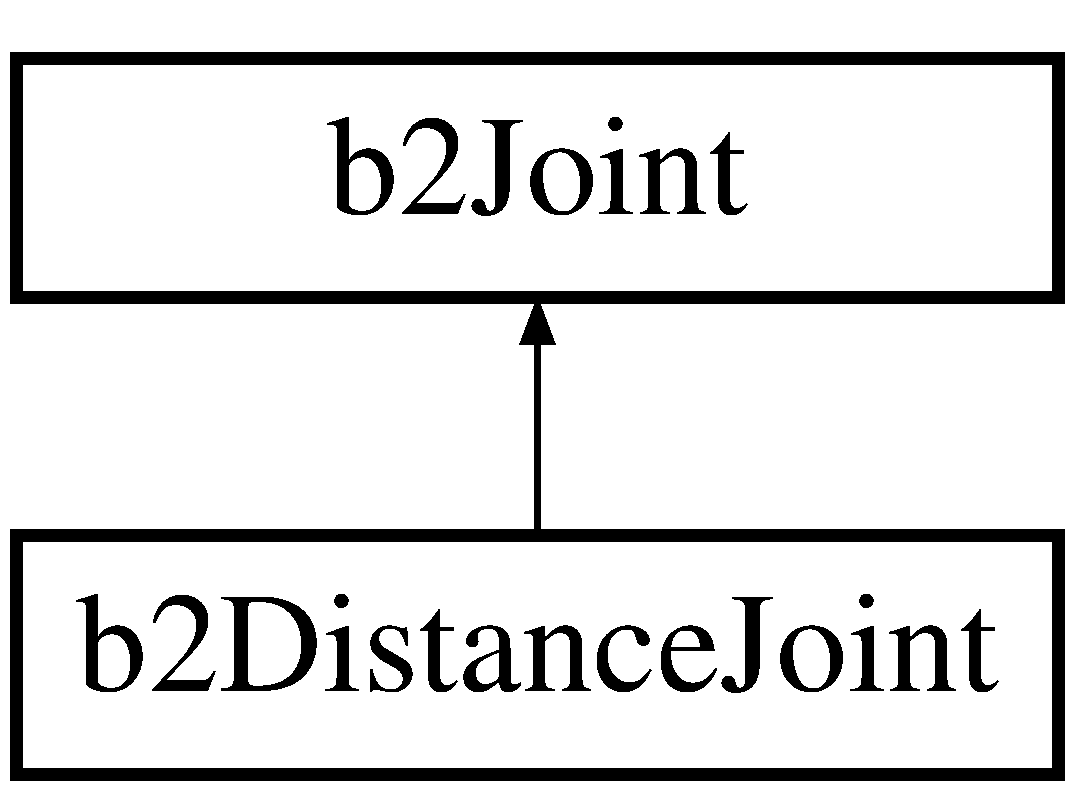
\includegraphics[height=2.000000cm]{classb2DistanceJoint}
\end{center}
\end{figure}
\subsection*{Public Member Functions}
\begin{DoxyCompactItemize}
\item 
\mbox{\Hypertarget{classb2DistanceJoint_ae228d3ce27009acd8a20c2570fb1183c}\label{classb2DistanceJoint_ae228d3ce27009acd8a20c2570fb1183c}} 
\mbox{\hyperlink{structb2Vec2}{b2\+Vec2}} \mbox{\hyperlink{classb2DistanceJoint_ae228d3ce27009acd8a20c2570fb1183c}{Get\+AnchorA}} () const override
\begin{DoxyCompactList}\small\item\em Get the anchor point on bodyA in world coordinates. \end{DoxyCompactList}\item 
\mbox{\Hypertarget{classb2DistanceJoint_a05bf71de10904c87e3a5295aa04a8aa6}\label{classb2DistanceJoint_a05bf71de10904c87e3a5295aa04a8aa6}} 
\mbox{\hyperlink{structb2Vec2}{b2\+Vec2}} \mbox{\hyperlink{classb2DistanceJoint_a05bf71de10904c87e3a5295aa04a8aa6}{Get\+AnchorB}} () const override
\begin{DoxyCompactList}\small\item\em Get the anchor point on bodyB in world coordinates. \end{DoxyCompactList}\item 
\mbox{\hyperlink{structb2Vec2}{b2\+Vec2}} \mbox{\hyperlink{classb2DistanceJoint_a6aa951e5bbfcae8a617987955cadbed5}{Get\+Reaction\+Force}} (float32 inv\+\_\+dt) const override
\item 
float32 \mbox{\hyperlink{classb2DistanceJoint_ad7ac78c4c20c122b944947d523a02982}{Get\+Reaction\+Torque}} (float32 inv\+\_\+dt) const override
\item 
\mbox{\Hypertarget{classb2DistanceJoint_aaa881128071c62f21898a75d5b20308a}\label{classb2DistanceJoint_aaa881128071c62f21898a75d5b20308a}} 
const \mbox{\hyperlink{structb2Vec2}{b2\+Vec2}} \& \mbox{\hyperlink{classb2DistanceJoint_aaa881128071c62f21898a75d5b20308a}{Get\+Local\+AnchorA}} () const
\begin{DoxyCompactList}\small\item\em The local anchor point relative to bodyA\textquotesingle{}s origin. \end{DoxyCompactList}\item 
\mbox{\Hypertarget{classb2DistanceJoint_a214a1cca8854613d7401c9a5892a28c9}\label{classb2DistanceJoint_a214a1cca8854613d7401c9a5892a28c9}} 
const \mbox{\hyperlink{structb2Vec2}{b2\+Vec2}} \& \mbox{\hyperlink{classb2DistanceJoint_a214a1cca8854613d7401c9a5892a28c9}{Get\+Local\+AnchorB}} () const
\begin{DoxyCompactList}\small\item\em The local anchor point relative to bodyB\textquotesingle{}s origin. \end{DoxyCompactList}\item 
void \mbox{\hyperlink{classb2DistanceJoint_a950a0f187ef691208e50de40ed9223fe}{Set\+Length}} (float32 length)
\item 
\mbox{\Hypertarget{classb2DistanceJoint_a7a4d8845e54abb6f8695ff6b3c78f9f9}\label{classb2DistanceJoint_a7a4d8845e54abb6f8695ff6b3c78f9f9}} 
float32 {\bfseries Get\+Length} () const
\item 
\mbox{\Hypertarget{classb2DistanceJoint_a1a12446f8926a1324edd481d9cd28c8a}\label{classb2DistanceJoint_a1a12446f8926a1324edd481d9cd28c8a}} 
void \mbox{\hyperlink{classb2DistanceJoint_a1a12446f8926a1324edd481d9cd28c8a}{Set\+Frequency}} (float32 hz)
\begin{DoxyCompactList}\small\item\em Set/get frequency in Hz. \end{DoxyCompactList}\item 
\mbox{\Hypertarget{classb2DistanceJoint_a9f7bfb48940bbc8dbef27600e327a739}\label{classb2DistanceJoint_a9f7bfb48940bbc8dbef27600e327a739}} 
float32 {\bfseries Get\+Frequency} () const
\item 
\mbox{\Hypertarget{classb2DistanceJoint_a58da61301a1f1398a715107b76649923}\label{classb2DistanceJoint_a58da61301a1f1398a715107b76649923}} 
void \mbox{\hyperlink{classb2DistanceJoint_a58da61301a1f1398a715107b76649923}{Set\+Damping\+Ratio}} (float32 ratio)
\begin{DoxyCompactList}\small\item\em Set/get damping ratio. \end{DoxyCompactList}\item 
\mbox{\Hypertarget{classb2DistanceJoint_a5c8ee3cfcadc356b957d71582b720056}\label{classb2DistanceJoint_a5c8ee3cfcadc356b957d71582b720056}} 
float32 {\bfseries Get\+Damping\+Ratio} () const
\item 
\mbox{\Hypertarget{classb2DistanceJoint_a3cebcc6ccce6f3c24432cd130fd53517}\label{classb2DistanceJoint_a3cebcc6ccce6f3c24432cd130fd53517}} 
void \mbox{\hyperlink{classb2DistanceJoint_a3cebcc6ccce6f3c24432cd130fd53517}{Dump}} ()
\begin{DoxyCompactList}\small\item\em Dump joint to dm\+Log. \end{DoxyCompactList}\end{DoxyCompactItemize}
\subsection*{Protected Member Functions}
\begin{DoxyCompactItemize}
\item 
\mbox{\Hypertarget{classb2DistanceJoint_ad2bb6de92a47868629a7397e23256454}\label{classb2DistanceJoint_ad2bb6de92a47868629a7397e23256454}} 
{\bfseries b2\+Distance\+Joint} (const \mbox{\hyperlink{structb2DistanceJointDef}{b2\+Distance\+Joint\+Def}} $\ast$data)
\item 
\mbox{\Hypertarget{classb2DistanceJoint_abe956dd5951651b36321098416ad99fd}\label{classb2DistanceJoint_abe956dd5951651b36321098416ad99fd}} 
void {\bfseries Init\+Velocity\+Constraints} (const \mbox{\hyperlink{structb2SolverData}{b2\+Solver\+Data}} \&data) override
\item 
\mbox{\Hypertarget{classb2DistanceJoint_ad42429151fb979a230f103d684d2a42c}\label{classb2DistanceJoint_ad42429151fb979a230f103d684d2a42c}} 
void {\bfseries Solve\+Velocity\+Constraints} (const \mbox{\hyperlink{structb2SolverData}{b2\+Solver\+Data}} \&data) override
\item 
\mbox{\Hypertarget{classb2DistanceJoint_a431d12fac5ee9f6a5637321ee28119bc}\label{classb2DistanceJoint_a431d12fac5ee9f6a5637321ee28119bc}} 
bool {\bfseries Solve\+Position\+Constraints} (const \mbox{\hyperlink{structb2SolverData}{b2\+Solver\+Data}} \&data) override
\end{DoxyCompactItemize}
\subsection*{Protected Attributes}
\begin{DoxyCompactItemize}
\item 
\mbox{\Hypertarget{classb2DistanceJoint_a90327211c322fa19ea7b8c58d0c27ea8}\label{classb2DistanceJoint_a90327211c322fa19ea7b8c58d0c27ea8}} 
float32 {\bfseries m\+\_\+frequency\+Hz}
\item 
\mbox{\Hypertarget{classb2DistanceJoint_a1339d37474c5e66cd4f66d42e9440307}\label{classb2DistanceJoint_a1339d37474c5e66cd4f66d42e9440307}} 
float32 {\bfseries m\+\_\+damping\+Ratio}
\item 
\mbox{\Hypertarget{classb2DistanceJoint_a91f829c0a95e0d5f204a512a506e29f0}\label{classb2DistanceJoint_a91f829c0a95e0d5f204a512a506e29f0}} 
float32 {\bfseries m\+\_\+bias}
\item 
\mbox{\Hypertarget{classb2DistanceJoint_a297938125dd60175ab07921d5ecc43a8}\label{classb2DistanceJoint_a297938125dd60175ab07921d5ecc43a8}} 
\mbox{\hyperlink{structb2Vec2}{b2\+Vec2}} {\bfseries m\+\_\+local\+AnchorA}
\item 
\mbox{\Hypertarget{classb2DistanceJoint_ad4c94a5b939ca4c3244bbab8544b880e}\label{classb2DistanceJoint_ad4c94a5b939ca4c3244bbab8544b880e}} 
\mbox{\hyperlink{structb2Vec2}{b2\+Vec2}} {\bfseries m\+\_\+local\+AnchorB}
\item 
\mbox{\Hypertarget{classb2DistanceJoint_a0ca755fb59c838c59d0ad162af8ab484}\label{classb2DistanceJoint_a0ca755fb59c838c59d0ad162af8ab484}} 
float32 {\bfseries m\+\_\+gamma}
\item 
\mbox{\Hypertarget{classb2DistanceJoint_a75713391126d712f728d1a4f33b32a9f}\label{classb2DistanceJoint_a75713391126d712f728d1a4f33b32a9f}} 
float32 {\bfseries m\+\_\+impulse}
\item 
\mbox{\Hypertarget{classb2DistanceJoint_a11b4805df34c380f53c3c346dd33da6c}\label{classb2DistanceJoint_a11b4805df34c380f53c3c346dd33da6c}} 
float32 {\bfseries m\+\_\+length}
\item 
\mbox{\Hypertarget{classb2DistanceJoint_abcae00902974ed826f70aa119c2fd9de}\label{classb2DistanceJoint_abcae00902974ed826f70aa119c2fd9de}} 
int32 {\bfseries m\+\_\+indexA}
\item 
\mbox{\Hypertarget{classb2DistanceJoint_a465f7f1b609bcb37be732cde71b6d8c8}\label{classb2DistanceJoint_a465f7f1b609bcb37be732cde71b6d8c8}} 
int32 {\bfseries m\+\_\+indexB}
\item 
\mbox{\Hypertarget{classb2DistanceJoint_a78f45f86d3cf68701a0871e9de71fcd0}\label{classb2DistanceJoint_a78f45f86d3cf68701a0871e9de71fcd0}} 
\mbox{\hyperlink{structb2Vec2}{b2\+Vec2}} {\bfseries m\+\_\+u}
\item 
\mbox{\Hypertarget{classb2DistanceJoint_af046e84218d249f9234a16ecab95bac0}\label{classb2DistanceJoint_af046e84218d249f9234a16ecab95bac0}} 
\mbox{\hyperlink{structb2Vec2}{b2\+Vec2}} {\bfseries m\+\_\+rA}
\item 
\mbox{\Hypertarget{classb2DistanceJoint_a70eab22cb7abeb825744f5dc3befa63a}\label{classb2DistanceJoint_a70eab22cb7abeb825744f5dc3befa63a}} 
\mbox{\hyperlink{structb2Vec2}{b2\+Vec2}} {\bfseries m\+\_\+rB}
\item 
\mbox{\Hypertarget{classb2DistanceJoint_a5793083e9ef396cf7a89d84481fe1308}\label{classb2DistanceJoint_a5793083e9ef396cf7a89d84481fe1308}} 
\mbox{\hyperlink{structb2Vec2}{b2\+Vec2}} {\bfseries m\+\_\+local\+CenterA}
\item 
\mbox{\Hypertarget{classb2DistanceJoint_a4fa600dec301992ad1f23aaf25d592a5}\label{classb2DistanceJoint_a4fa600dec301992ad1f23aaf25d592a5}} 
\mbox{\hyperlink{structb2Vec2}{b2\+Vec2}} {\bfseries m\+\_\+local\+CenterB}
\item 
\mbox{\Hypertarget{classb2DistanceJoint_a2564d44d59b589591a4214390617cc4e}\label{classb2DistanceJoint_a2564d44d59b589591a4214390617cc4e}} 
float32 {\bfseries m\+\_\+inv\+MassA}
\item 
\mbox{\Hypertarget{classb2DistanceJoint_aeaea63222b01f95c71da5719feca4cbc}\label{classb2DistanceJoint_aeaea63222b01f95c71da5719feca4cbc}} 
float32 {\bfseries m\+\_\+inv\+MassB}
\item 
\mbox{\Hypertarget{classb2DistanceJoint_a9e9edc41d2bf14189a3eaeb19995b93a}\label{classb2DistanceJoint_a9e9edc41d2bf14189a3eaeb19995b93a}} 
float32 {\bfseries m\+\_\+inv\+IA}
\item 
\mbox{\Hypertarget{classb2DistanceJoint_a250b46aa3fc17a363a6af9af5749ce1c}\label{classb2DistanceJoint_a250b46aa3fc17a363a6af9af5749ce1c}} 
float32 {\bfseries m\+\_\+inv\+IB}
\item 
\mbox{\Hypertarget{classb2DistanceJoint_aee25a31b1096e91b55a29731cf67d99d}\label{classb2DistanceJoint_aee25a31b1096e91b55a29731cf67d99d}} 
float32 {\bfseries m\+\_\+mass}
\end{DoxyCompactItemize}
\subsection*{Friends}
\begin{DoxyCompactItemize}
\item 
\mbox{\Hypertarget{classb2DistanceJoint_a54ade8ed3d794298108d7f4c4e4793fa}\label{classb2DistanceJoint_a54ade8ed3d794298108d7f4c4e4793fa}} 
class {\bfseries b2\+Joint}
\end{DoxyCompactItemize}
\subsection*{Additional Inherited Members}


\subsection{Detailed Description}
A distance joint constrains two points on two bodies to remain at a fixed distance from each other. You can view this as a massless, rigid rod. 

\subsection{Member Function Documentation}
\mbox{\Hypertarget{classb2DistanceJoint_a6aa951e5bbfcae8a617987955cadbed5}\label{classb2DistanceJoint_a6aa951e5bbfcae8a617987955cadbed5}} 
\index{b2\+Distance\+Joint@{b2\+Distance\+Joint}!Get\+Reaction\+Force@{Get\+Reaction\+Force}}
\index{Get\+Reaction\+Force@{Get\+Reaction\+Force}!b2\+Distance\+Joint@{b2\+Distance\+Joint}}
\subsubsection{\texorpdfstring{Get\+Reaction\+Force()}{GetReactionForce()}}
{\footnotesize\ttfamily \mbox{\hyperlink{structb2Vec2}{b2\+Vec2}} b2\+Distance\+Joint\+::\+Get\+Reaction\+Force (\begin{DoxyParamCaption}\item[{float32}]{inv\+\_\+dt }\end{DoxyParamCaption}) const\hspace{0.3cm}{\ttfamily [override]}, {\ttfamily [virtual]}}

Get the reaction force given the inverse time step. Unit is N. 

Implements \mbox{\hyperlink{classb2Joint_a7e0eddefb9b69ad050b8ef6425838a74}{b2\+Joint}}.

\mbox{\Hypertarget{classb2DistanceJoint_ad7ac78c4c20c122b944947d523a02982}\label{classb2DistanceJoint_ad7ac78c4c20c122b944947d523a02982}} 
\index{b2\+Distance\+Joint@{b2\+Distance\+Joint}!Get\+Reaction\+Torque@{Get\+Reaction\+Torque}}
\index{Get\+Reaction\+Torque@{Get\+Reaction\+Torque}!b2\+Distance\+Joint@{b2\+Distance\+Joint}}
\subsubsection{\texorpdfstring{Get\+Reaction\+Torque()}{GetReactionTorque()}}
{\footnotesize\ttfamily float32 b2\+Distance\+Joint\+::\+Get\+Reaction\+Torque (\begin{DoxyParamCaption}\item[{float32}]{inv\+\_\+dt }\end{DoxyParamCaption}) const\hspace{0.3cm}{\ttfamily [override]}, {\ttfamily [virtual]}}

Get the reaction torque given the inverse time step. Unit is N$\ast$m. This is always zero for a distance joint. 

Implements \mbox{\hyperlink{classb2Joint_ae355e441c2aa842777dc04e24f15ced0}{b2\+Joint}}.

\mbox{\Hypertarget{classb2DistanceJoint_a950a0f187ef691208e50de40ed9223fe}\label{classb2DistanceJoint_a950a0f187ef691208e50de40ed9223fe}} 
\index{b2\+Distance\+Joint@{b2\+Distance\+Joint}!Set\+Length@{Set\+Length}}
\index{Set\+Length@{Set\+Length}!b2\+Distance\+Joint@{b2\+Distance\+Joint}}
\subsubsection{\texorpdfstring{Set\+Length()}{SetLength()}}
{\footnotesize\ttfamily void b2\+Distance\+Joint\+::\+Set\+Length (\begin{DoxyParamCaption}\item[{float32}]{length }\end{DoxyParamCaption})\hspace{0.3cm}{\ttfamily [inline]}}

Set/get the natural length. Manipulating the length can lead to non-\/physical behavior when the frequency is zero. 

The documentation for this class was generated from the following files\+:\begin{DoxyCompactItemize}
\item 
Dynamics/\+Joints/b2\+Distance\+Joint.\+h\item 
Dynamics/\+Joints/b2\+Distance\+Joint.\+cpp\end{DoxyCompactItemize}

\hypertarget{structb2DistanceJointDef}{}\section{b2\+Distance\+Joint\+Def Struct Reference}
\label{structb2DistanceJointDef}\index{b2\+Distance\+Joint\+Def@{b2\+Distance\+Joint\+Def}}


{\ttfamily \#include $<$b2\+Distance\+Joint.\+h$>$}

Inheritance diagram for b2\+Distance\+Joint\+Def\+:\begin{figure}[H]
\begin{center}
\leavevmode
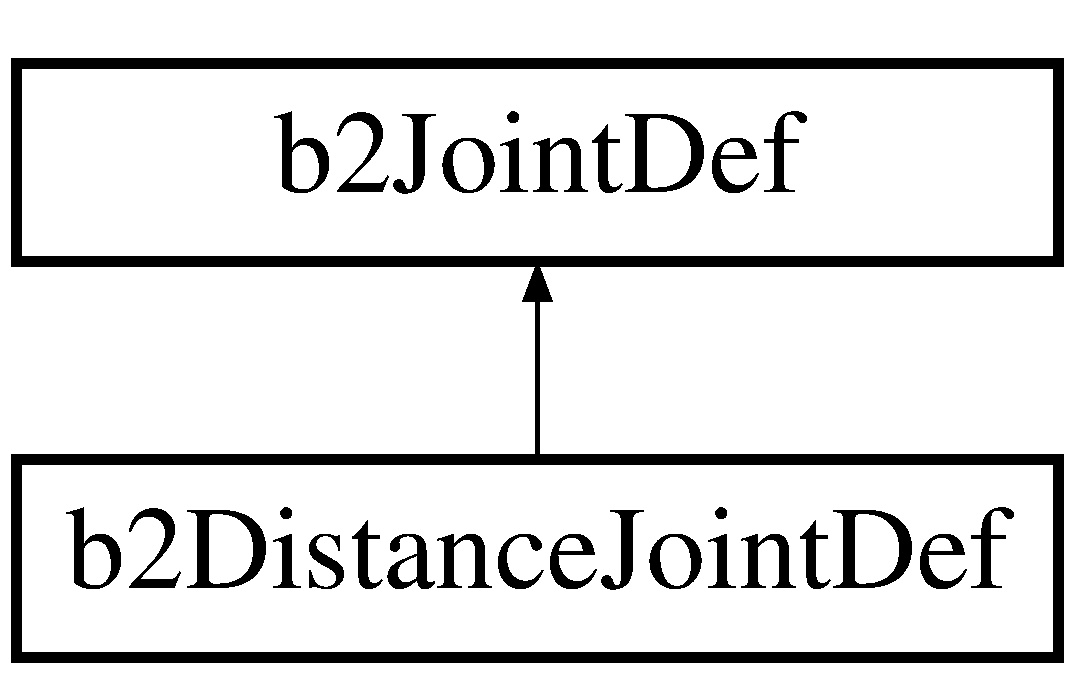
\includegraphics[height=2.000000cm]{structb2DistanceJointDef}
\end{center}
\end{figure}
\subsection*{Public Member Functions}
\begin{DoxyCompactItemize}
\item 
void \mbox{\hyperlink{structb2DistanceJointDef_a99788a534638cc28cd1e44e0036503f0}{Initialize}} (\mbox{\hyperlink{classb2Body}{b2\+Body}} $\ast$\mbox{\hyperlink{structb2JointDef_a8cd54c93da396be75a9788f2c6897f05}{bodyA}}, \mbox{\hyperlink{classb2Body}{b2\+Body}} $\ast$\mbox{\hyperlink{structb2JointDef_aa4f4dee2fbcd12187b19506b60e68e3d}{bodyB}}, const \mbox{\hyperlink{structb2Vec2}{b2\+Vec2}} \&anchorA, const \mbox{\hyperlink{structb2Vec2}{b2\+Vec2}} \&anchorB)
\end{DoxyCompactItemize}
\subsection*{Public Attributes}
\begin{DoxyCompactItemize}
\item 
\mbox{\Hypertarget{structb2DistanceJointDef_a15c7a75fa277e2056bf1b44198658518}\label{structb2DistanceJointDef_a15c7a75fa277e2056bf1b44198658518}} 
\mbox{\hyperlink{structb2Vec2}{b2\+Vec2}} \mbox{\hyperlink{structb2DistanceJointDef_a15c7a75fa277e2056bf1b44198658518}{local\+AnchorA}}
\begin{DoxyCompactList}\small\item\em The local anchor point relative to bodyA\textquotesingle{}s origin. \end{DoxyCompactList}\item 
\mbox{\Hypertarget{structb2DistanceJointDef_a3c8995be726238eee084af750442255c}\label{structb2DistanceJointDef_a3c8995be726238eee084af750442255c}} 
\mbox{\hyperlink{structb2Vec2}{b2\+Vec2}} \mbox{\hyperlink{structb2DistanceJointDef_a3c8995be726238eee084af750442255c}{local\+AnchorB}}
\begin{DoxyCompactList}\small\item\em The local anchor point relative to bodyB\textquotesingle{}s origin. \end{DoxyCompactList}\item 
\mbox{\Hypertarget{structb2DistanceJointDef_ac2c48ad52de91c804c386c12c5bf3714}\label{structb2DistanceJointDef_ac2c48ad52de91c804c386c12c5bf3714}} 
float32 \mbox{\hyperlink{structb2DistanceJointDef_ac2c48ad52de91c804c386c12c5bf3714}{length}}
\begin{DoxyCompactList}\small\item\em The natural length between the anchor points. \end{DoxyCompactList}\item 
float32 \mbox{\hyperlink{structb2DistanceJointDef_a35e2362bcb6c58734f95d0ac045863ea}{frequency\+Hz}}
\item 
\mbox{\Hypertarget{structb2DistanceJointDef_ad009b24ff211158eb4e1db4815a63b94}\label{structb2DistanceJointDef_ad009b24ff211158eb4e1db4815a63b94}} 
float32 \mbox{\hyperlink{structb2DistanceJointDef_ad009b24ff211158eb4e1db4815a63b94}{damping\+Ratio}}
\begin{DoxyCompactList}\small\item\em The damping ratio. 0 = no damping, 1 = critical damping. \end{DoxyCompactList}\end{DoxyCompactItemize}


\subsection{Detailed Description}
Distance joint definition. This requires defining an anchor point on both bodies and the non-\/zero length of the distance joint. The definition uses local anchor points so that the initial configuration can violate the constraint slightly. This helps when saving and loading a game. \begin{DoxyWarning}{Warning}
Do not use a zero or short length. 
\end{DoxyWarning}


\subsection{Member Function Documentation}
\mbox{\Hypertarget{structb2DistanceJointDef_a99788a534638cc28cd1e44e0036503f0}\label{structb2DistanceJointDef_a99788a534638cc28cd1e44e0036503f0}} 
\index{b2\+Distance\+Joint\+Def@{b2\+Distance\+Joint\+Def}!Initialize@{Initialize}}
\index{Initialize@{Initialize}!b2\+Distance\+Joint\+Def@{b2\+Distance\+Joint\+Def}}
\subsubsection{\texorpdfstring{Initialize()}{Initialize()}}
{\footnotesize\ttfamily void b2\+Distance\+Joint\+Def\+::\+Initialize (\begin{DoxyParamCaption}\item[{\mbox{\hyperlink{classb2Body}{b2\+Body}} $\ast$}]{bodyA,  }\item[{\mbox{\hyperlink{classb2Body}{b2\+Body}} $\ast$}]{bodyB,  }\item[{const \mbox{\hyperlink{structb2Vec2}{b2\+Vec2}} \&}]{anchorA,  }\item[{const \mbox{\hyperlink{structb2Vec2}{b2\+Vec2}} \&}]{anchorB }\end{DoxyParamCaption})}

Initialize the bodies, anchors, and length using the world anchors. 

\subsection{Member Data Documentation}
\mbox{\Hypertarget{structb2DistanceJointDef_a35e2362bcb6c58734f95d0ac045863ea}\label{structb2DistanceJointDef_a35e2362bcb6c58734f95d0ac045863ea}} 
\index{b2\+Distance\+Joint\+Def@{b2\+Distance\+Joint\+Def}!frequency\+Hz@{frequency\+Hz}}
\index{frequency\+Hz@{frequency\+Hz}!b2\+Distance\+Joint\+Def@{b2\+Distance\+Joint\+Def}}
\subsubsection{\texorpdfstring{frequency\+Hz}{frequencyHz}}
{\footnotesize\ttfamily float32 b2\+Distance\+Joint\+Def\+::frequency\+Hz}

The mass-\/spring-\/damper frequency in Hertz. A value of 0 disables softness. 

The documentation for this struct was generated from the following files\+:\begin{DoxyCompactItemize}
\item 
Dynamics/\+Joints/b2\+Distance\+Joint.\+h\item 
Dynamics/\+Joints/b2\+Distance\+Joint.\+cpp\end{DoxyCompactItemize}

\hypertarget{structb2DistanceOutput}{}\section{b2\+Distance\+Output Struct Reference}
\label{structb2DistanceOutput}\index{b2\+Distance\+Output@{b2\+Distance\+Output}}


Output for b2\+Distance.  




{\ttfamily \#include $<$b2\+Distance.\+h$>$}

\subsection*{Public Attributes}
\begin{DoxyCompactItemize}
\item 
\mbox{\Hypertarget{structb2DistanceOutput_a7e0f1f44a64e596dc7d37570c69eefce}\label{structb2DistanceOutput_a7e0f1f44a64e596dc7d37570c69eefce}} 
\mbox{\hyperlink{structb2Vec2}{b2\+Vec2}} \mbox{\hyperlink{structb2DistanceOutput_a7e0f1f44a64e596dc7d37570c69eefce}{pointA}}
\begin{DoxyCompactList}\small\item\em closest point on shapeA \end{DoxyCompactList}\item 
\mbox{\Hypertarget{structb2DistanceOutput_aa85beca17337a506cd4a924d0c6f92cc}\label{structb2DistanceOutput_aa85beca17337a506cd4a924d0c6f92cc}} 
\mbox{\hyperlink{structb2Vec2}{b2\+Vec2}} \mbox{\hyperlink{structb2DistanceOutput_aa85beca17337a506cd4a924d0c6f92cc}{pointB}}
\begin{DoxyCompactList}\small\item\em closest point on shapeB \end{DoxyCompactList}\item 
\mbox{\Hypertarget{structb2DistanceOutput_ae67f480ff37d4ab732e6366f485c7f55}\label{structb2DistanceOutput_ae67f480ff37d4ab732e6366f485c7f55}} 
float32 {\bfseries distance}
\item 
\mbox{\Hypertarget{structb2DistanceOutput_ae2d4c84dd3d05ea4f4d20c91099ec8d5}\label{structb2DistanceOutput_ae2d4c84dd3d05ea4f4d20c91099ec8d5}} 
int32 \mbox{\hyperlink{structb2DistanceOutput_ae2d4c84dd3d05ea4f4d20c91099ec8d5}{iterations}}
\begin{DoxyCompactList}\small\item\em number of G\+JK iterations used \end{DoxyCompactList}\end{DoxyCompactItemize}


\subsection{Detailed Description}
Output for b2\+Distance. 

The documentation for this struct was generated from the following file\+:\begin{DoxyCompactItemize}
\item 
Collision/b2\+Distance.\+h\end{DoxyCompactItemize}

\hypertarget{structb2DistanceProxy}{}\section{b2\+Distance\+Proxy Struct Reference}
\label{structb2DistanceProxy}\index{b2\+Distance\+Proxy@{b2\+Distance\+Proxy}}


{\ttfamily \#include $<$b2\+Distance.\+h$>$}

\subsection*{Public Member Functions}
\begin{DoxyCompactItemize}
\item 
void \mbox{\hyperlink{structb2DistanceProxy_a80a59a9c9e952482a8fc6db4b883365d}{Set}} (const \mbox{\hyperlink{classb2Shape}{b2\+Shape}} $\ast$shape, int32 index)
\item 
\mbox{\Hypertarget{structb2DistanceProxy_a39de286cc0c1e829adfacfa0061b04f2}\label{structb2DistanceProxy_a39de286cc0c1e829adfacfa0061b04f2}} 
int32 \mbox{\hyperlink{structb2DistanceProxy_a39de286cc0c1e829adfacfa0061b04f2}{Get\+Support}} (const \mbox{\hyperlink{structb2Vec2}{b2\+Vec2}} \&d) const
\begin{DoxyCompactList}\small\item\em Get the supporting vertex index in the given direction. \end{DoxyCompactList}\item 
\mbox{\Hypertarget{structb2DistanceProxy_a245993f09e9f3d3f374bb95041acf822}\label{structb2DistanceProxy_a245993f09e9f3d3f374bb95041acf822}} 
const \mbox{\hyperlink{structb2Vec2}{b2\+Vec2}} \& \mbox{\hyperlink{structb2DistanceProxy_a245993f09e9f3d3f374bb95041acf822}{Get\+Support\+Vertex}} (const \mbox{\hyperlink{structb2Vec2}{b2\+Vec2}} \&d) const
\begin{DoxyCompactList}\small\item\em Get the supporting vertex in the given direction. \end{DoxyCompactList}\item 
\mbox{\Hypertarget{structb2DistanceProxy_a99c461f28d484429dac8f14b58f63d89}\label{structb2DistanceProxy_a99c461f28d484429dac8f14b58f63d89}} 
int32 \mbox{\hyperlink{structb2DistanceProxy_a99c461f28d484429dac8f14b58f63d89}{Get\+Vertex\+Count}} () const
\begin{DoxyCompactList}\small\item\em Get the vertex count. \end{DoxyCompactList}\item 
\mbox{\Hypertarget{structb2DistanceProxy_a9073b2c680d3fee6399f15be79ad144a}\label{structb2DistanceProxy_a9073b2c680d3fee6399f15be79ad144a}} 
const \mbox{\hyperlink{structb2Vec2}{b2\+Vec2}} \& \mbox{\hyperlink{structb2DistanceProxy_a9073b2c680d3fee6399f15be79ad144a}{Get\+Vertex}} (int32 index) const
\begin{DoxyCompactList}\small\item\em Get a vertex by index. Used by b2\+Distance. \end{DoxyCompactList}\end{DoxyCompactItemize}
\subsection*{Public Attributes}
\begin{DoxyCompactItemize}
\item 
\mbox{\Hypertarget{structb2DistanceProxy_a3fc5ebfa3d34ac66390b88f9277fb330}\label{structb2DistanceProxy_a3fc5ebfa3d34ac66390b88f9277fb330}} 
\mbox{\hyperlink{structb2Vec2}{b2\+Vec2}} {\bfseries m\+\_\+buffer} \mbox{[}2\mbox{]}
\item 
\mbox{\Hypertarget{structb2DistanceProxy_abaf1495b8214b74d944b57170a762f32}\label{structb2DistanceProxy_abaf1495b8214b74d944b57170a762f32}} 
const \mbox{\hyperlink{structb2Vec2}{b2\+Vec2}} $\ast$ {\bfseries m\+\_\+vertices}
\item 
\mbox{\Hypertarget{structb2DistanceProxy_ae36efab1361bb1f94e32f9b956c6f1b3}\label{structb2DistanceProxy_ae36efab1361bb1f94e32f9b956c6f1b3}} 
int32 {\bfseries m\+\_\+count}
\item 
\mbox{\Hypertarget{structb2DistanceProxy_a459c93f35b1e62d583bd73d8c478ce89}\label{structb2DistanceProxy_a459c93f35b1e62d583bd73d8c478ce89}} 
float32 {\bfseries m\+\_\+radius}
\end{DoxyCompactItemize}


\subsection{Detailed Description}
A distance proxy is used by the G\+JK algorithm. It encapsulates any shape. 

\subsection{Member Function Documentation}
\mbox{\Hypertarget{structb2DistanceProxy_a80a59a9c9e952482a8fc6db4b883365d}\label{structb2DistanceProxy_a80a59a9c9e952482a8fc6db4b883365d}} 
\index{b2\+Distance\+Proxy@{b2\+Distance\+Proxy}!Set@{Set}}
\index{Set@{Set}!b2\+Distance\+Proxy@{b2\+Distance\+Proxy}}
\subsubsection{\texorpdfstring{Set()}{Set()}}
{\footnotesize\ttfamily void b2\+Distance\+Proxy\+::\+Set (\begin{DoxyParamCaption}\item[{const \mbox{\hyperlink{classb2Shape}{b2\+Shape}} $\ast$}]{shape,  }\item[{int32}]{index }\end{DoxyParamCaption})}

Initialize the proxy using the given shape. The shape must remain in scope while the proxy is in use. 

The documentation for this struct was generated from the following files\+:\begin{DoxyCompactItemize}
\item 
Collision/b2\+Distance.\+h\item 
Collision/b2\+Distance.\+cpp\end{DoxyCompactItemize}

\hypertarget{classb2Draw}{}\section{b2\+Draw Class Reference}
\label{classb2Draw}\index{b2\+Draw@{b2\+Draw}}


{\ttfamily \#include $<$b2\+Draw.\+h$>$}

\subsection*{Public Types}
\begin{DoxyCompactItemize}
\item 
enum \{ \newline
\mbox{\hyperlink{classb2Draw_ae23c5d6c4f5230621f736593469cf7f2a1c8964c4f1fdc39e98b58ac38ecda1f9}{e\+\_\+shape\+Bit}} = 0x0001, 
\mbox{\hyperlink{classb2Draw_ae23c5d6c4f5230621f736593469cf7f2a241137a63679720c41a271c11681e2b3}{e\+\_\+joint\+Bit}} = 0x0002, 
\mbox{\hyperlink{classb2Draw_ae23c5d6c4f5230621f736593469cf7f2acdf1370108930182a45f39e7cc9b0cc7}{e\+\_\+aabb\+Bit}} = 0x0004, 
\mbox{\hyperlink{classb2Draw_ae23c5d6c4f5230621f736593469cf7f2ac86bb64ac65e555db28827407f2f2d43}{e\+\_\+pair\+Bit}} = 0x0008, 
\newline
\mbox{\hyperlink{classb2Draw_ae23c5d6c4f5230621f736593469cf7f2a7f1494d816479c7d23997a6c292cd8b6}{e\+\_\+center\+Of\+Mass\+Bit}} = 0x0010
 \}
\end{DoxyCompactItemize}
\subsection*{Public Member Functions}
\begin{DoxyCompactItemize}
\item 
\mbox{\Hypertarget{classb2Draw_ac2bbe31595478690e44de4ff1e7f347e}\label{classb2Draw_ac2bbe31595478690e44de4ff1e7f347e}} 
void \mbox{\hyperlink{classb2Draw_ac2bbe31595478690e44de4ff1e7f347e}{Set\+Flags}} (uint32 flags)
\begin{DoxyCompactList}\small\item\em Set the drawing flags. \end{DoxyCompactList}\item 
\mbox{\Hypertarget{classb2Draw_a10926d67ad6d3a2517197c4f10923700}\label{classb2Draw_a10926d67ad6d3a2517197c4f10923700}} 
uint32 \mbox{\hyperlink{classb2Draw_a10926d67ad6d3a2517197c4f10923700}{Get\+Flags}} () const
\begin{DoxyCompactList}\small\item\em Get the drawing flags. \end{DoxyCompactList}\item 
\mbox{\Hypertarget{classb2Draw_acc2fd4648ee0a65574770c64528f7166}\label{classb2Draw_acc2fd4648ee0a65574770c64528f7166}} 
void \mbox{\hyperlink{classb2Draw_acc2fd4648ee0a65574770c64528f7166}{Append\+Flags}} (uint32 flags)
\begin{DoxyCompactList}\small\item\em Append flags to the current flags. \end{DoxyCompactList}\item 
\mbox{\Hypertarget{classb2Draw_afc240b71f4ba8c17440d6ed526d4e22e}\label{classb2Draw_afc240b71f4ba8c17440d6ed526d4e22e}} 
void \mbox{\hyperlink{classb2Draw_afc240b71f4ba8c17440d6ed526d4e22e}{Clear\+Flags}} (uint32 flags)
\begin{DoxyCompactList}\small\item\em Clear flags from the current flags. \end{DoxyCompactList}\item 
\mbox{\Hypertarget{classb2Draw_acd5427d1d2e7d19f1b34ad3620134d28}\label{classb2Draw_acd5427d1d2e7d19f1b34ad3620134d28}} 
virtual void \mbox{\hyperlink{classb2Draw_acd5427d1d2e7d19f1b34ad3620134d28}{Draw\+Polygon}} (const \mbox{\hyperlink{structb2Vec2}{b2\+Vec2}} $\ast$vertices, int32 vertex\+Count, const \mbox{\hyperlink{structb2Color}{b2\+Color}} \&color)=0
\begin{DoxyCompactList}\small\item\em Draw a closed polygon provided in C\+CW order. \end{DoxyCompactList}\item 
\mbox{\Hypertarget{classb2Draw_a76f2d67de0781a32cab116278c5c9eea}\label{classb2Draw_a76f2d67de0781a32cab116278c5c9eea}} 
virtual void \mbox{\hyperlink{classb2Draw_a76f2d67de0781a32cab116278c5c9eea}{Draw\+Solid\+Polygon}} (const \mbox{\hyperlink{structb2Vec2}{b2\+Vec2}} $\ast$vertices, int32 vertex\+Count, const \mbox{\hyperlink{structb2Color}{b2\+Color}} \&color)=0
\begin{DoxyCompactList}\small\item\em Draw a solid closed polygon provided in C\+CW order. \end{DoxyCompactList}\item 
\mbox{\Hypertarget{classb2Draw_ae2effe9bca87c8d7cb90e860d13b7e9e}\label{classb2Draw_ae2effe9bca87c8d7cb90e860d13b7e9e}} 
virtual void \mbox{\hyperlink{classb2Draw_ae2effe9bca87c8d7cb90e860d13b7e9e}{Draw\+Circle}} (const \mbox{\hyperlink{structb2Vec2}{b2\+Vec2}} \&center, float32 radius, const \mbox{\hyperlink{structb2Color}{b2\+Color}} \&color)=0
\begin{DoxyCompactList}\small\item\em Draw a circle. \end{DoxyCompactList}\item 
\mbox{\Hypertarget{classb2Draw_a775a1d0472c5980d597904c7b596a0a6}\label{classb2Draw_a775a1d0472c5980d597904c7b596a0a6}} 
virtual void \mbox{\hyperlink{classb2Draw_a775a1d0472c5980d597904c7b596a0a6}{Draw\+Solid\+Circle}} (const \mbox{\hyperlink{structb2Vec2}{b2\+Vec2}} \&center, float32 radius, const \mbox{\hyperlink{structb2Vec2}{b2\+Vec2}} \&axis, const \mbox{\hyperlink{structb2Color}{b2\+Color}} \&color)=0
\begin{DoxyCompactList}\small\item\em Draw a solid circle. \end{DoxyCompactList}\item 
\mbox{\Hypertarget{classb2Draw_a1de5aaf50db875d1c644c596832af57d}\label{classb2Draw_a1de5aaf50db875d1c644c596832af57d}} 
virtual void \mbox{\hyperlink{classb2Draw_a1de5aaf50db875d1c644c596832af57d}{Draw\+Segment}} (const \mbox{\hyperlink{structb2Vec2}{b2\+Vec2}} \&p1, const \mbox{\hyperlink{structb2Vec2}{b2\+Vec2}} \&p2, const \mbox{\hyperlink{structb2Color}{b2\+Color}} \&color)=0
\begin{DoxyCompactList}\small\item\em Draw a line segment. \end{DoxyCompactList}\item 
virtual void \mbox{\hyperlink{classb2Draw_ade698123482a491a7a61fa1fe4d3a4f4}{Draw\+Transform}} (const \mbox{\hyperlink{structb2Transform}{b2\+Transform}} \&xf)=0
\item 
\mbox{\Hypertarget{classb2Draw_acc83934a18c276d4391296c4968d9e16}\label{classb2Draw_acc83934a18c276d4391296c4968d9e16}} 
virtual void \mbox{\hyperlink{classb2Draw_acc83934a18c276d4391296c4968d9e16}{Draw\+Point}} (const \mbox{\hyperlink{structb2Vec2}{b2\+Vec2}} \&p, float32 size, const \mbox{\hyperlink{structb2Color}{b2\+Color}} \&color)=0
\begin{DoxyCompactList}\small\item\em Draw a point. \end{DoxyCompactList}\end{DoxyCompactItemize}
\subsection*{Protected Attributes}
\begin{DoxyCompactItemize}
\item 
\mbox{\Hypertarget{classb2Draw_adfcd2e54ddaec6f0a111ec1a1cf8b9a0}\label{classb2Draw_adfcd2e54ddaec6f0a111ec1a1cf8b9a0}} 
uint32 {\bfseries m\+\_\+draw\+Flags}
\end{DoxyCompactItemize}


\subsection{Detailed Description}
Implement and register this class with a \mbox{\hyperlink{classb2World}{b2\+World}} to provide debug drawing of physics entities in your game. 

\subsection{Member Enumeration Documentation}
\mbox{\Hypertarget{classb2Draw_ae23c5d6c4f5230621f736593469cf7f2}\label{classb2Draw_ae23c5d6c4f5230621f736593469cf7f2}} 
\subsubsection{\texorpdfstring{anonymous enum}{anonymous enum}}
{\footnotesize\ttfamily anonymous enum}

\begin{DoxyEnumFields}{Enumerator}
\raisebox{\heightof{T}}[0pt][0pt]{\index{e\+\_\+shape\+Bit@{e\+\_\+shape\+Bit}!b2\+Draw@{b2\+Draw}}\index{b2\+Draw@{b2\+Draw}!e\+\_\+shape\+Bit@{e\+\_\+shape\+Bit}}}\mbox{\Hypertarget{classb2Draw_ae23c5d6c4f5230621f736593469cf7f2a1c8964c4f1fdc39e98b58ac38ecda1f9}\label{classb2Draw_ae23c5d6c4f5230621f736593469cf7f2a1c8964c4f1fdc39e98b58ac38ecda1f9}} 
e\+\_\+shape\+Bit&draw shapes \\
\hline

\raisebox{\heightof{T}}[0pt][0pt]{\index{e\+\_\+joint\+Bit@{e\+\_\+joint\+Bit}!b2\+Draw@{b2\+Draw}}\index{b2\+Draw@{b2\+Draw}!e\+\_\+joint\+Bit@{e\+\_\+joint\+Bit}}}\mbox{\Hypertarget{classb2Draw_ae23c5d6c4f5230621f736593469cf7f2a241137a63679720c41a271c11681e2b3}\label{classb2Draw_ae23c5d6c4f5230621f736593469cf7f2a241137a63679720c41a271c11681e2b3}} 
e\+\_\+joint\+Bit&draw joint connections \\
\hline

\raisebox{\heightof{T}}[0pt][0pt]{\index{e\+\_\+aabb\+Bit@{e\+\_\+aabb\+Bit}!b2\+Draw@{b2\+Draw}}\index{b2\+Draw@{b2\+Draw}!e\+\_\+aabb\+Bit@{e\+\_\+aabb\+Bit}}}\mbox{\Hypertarget{classb2Draw_ae23c5d6c4f5230621f736593469cf7f2acdf1370108930182a45f39e7cc9b0cc7}\label{classb2Draw_ae23c5d6c4f5230621f736593469cf7f2acdf1370108930182a45f39e7cc9b0cc7}} 
e\+\_\+aabb\+Bit&draw axis aligned bounding boxes \\
\hline

\raisebox{\heightof{T}}[0pt][0pt]{\index{e\+\_\+pair\+Bit@{e\+\_\+pair\+Bit}!b2\+Draw@{b2\+Draw}}\index{b2\+Draw@{b2\+Draw}!e\+\_\+pair\+Bit@{e\+\_\+pair\+Bit}}}\mbox{\Hypertarget{classb2Draw_ae23c5d6c4f5230621f736593469cf7f2ac86bb64ac65e555db28827407f2f2d43}\label{classb2Draw_ae23c5d6c4f5230621f736593469cf7f2ac86bb64ac65e555db28827407f2f2d43}} 
e\+\_\+pair\+Bit&draw broad-\/phase pairs \\
\hline

\raisebox{\heightof{T}}[0pt][0pt]{\index{e\+\_\+center\+Of\+Mass\+Bit@{e\+\_\+center\+Of\+Mass\+Bit}!b2\+Draw@{b2\+Draw}}\index{b2\+Draw@{b2\+Draw}!e\+\_\+center\+Of\+Mass\+Bit@{e\+\_\+center\+Of\+Mass\+Bit}}}\mbox{\Hypertarget{classb2Draw_ae23c5d6c4f5230621f736593469cf7f2a7f1494d816479c7d23997a6c292cd8b6}\label{classb2Draw_ae23c5d6c4f5230621f736593469cf7f2a7f1494d816479c7d23997a6c292cd8b6}} 
e\+\_\+center\+Of\+Mass\+Bit&draw center of mass frame \\
\hline

\end{DoxyEnumFields}


\subsection{Member Function Documentation}
\mbox{\Hypertarget{classb2Draw_ade698123482a491a7a61fa1fe4d3a4f4}\label{classb2Draw_ade698123482a491a7a61fa1fe4d3a4f4}} 
\index{b2\+Draw@{b2\+Draw}!Draw\+Transform@{Draw\+Transform}}
\index{Draw\+Transform@{Draw\+Transform}!b2\+Draw@{b2\+Draw}}
\subsubsection{\texorpdfstring{Draw\+Transform()}{DrawTransform()}}
{\footnotesize\ttfamily virtual void b2\+Draw\+::\+Draw\+Transform (\begin{DoxyParamCaption}\item[{const \mbox{\hyperlink{structb2Transform}{b2\+Transform}} \&}]{xf }\end{DoxyParamCaption})\hspace{0.3cm}{\ttfamily [pure virtual]}}

Draw a transform. Choose your own length scale. 
\begin{DoxyParams}{Parameters}
{\em xf} & a transform. \\
\hline
\end{DoxyParams}


The documentation for this class was generated from the following files\+:\begin{DoxyCompactItemize}
\item 
Common/b2\+Draw.\+h\item 
Common/b2\+Draw.\+cpp\end{DoxyCompactItemize}

\hypertarget{classb2DynamicTree}{}\section{b2\+Dynamic\+Tree Class Reference}
\label{classb2DynamicTree}\index{b2\+Dynamic\+Tree@{b2\+Dynamic\+Tree}}


{\ttfamily \#include $<$b2\+Dynamic\+Tree.\+h$>$}

\subsection*{Public Member Functions}
\begin{DoxyCompactItemize}
\item 
\mbox{\Hypertarget{classb2DynamicTree_a8af64cf6a1566fa4c5b5c9683bd937d9}\label{classb2DynamicTree_a8af64cf6a1566fa4c5b5c9683bd937d9}} 
\mbox{\hyperlink{classb2DynamicTree_a8af64cf6a1566fa4c5b5c9683bd937d9}{b2\+Dynamic\+Tree}} ()
\begin{DoxyCompactList}\small\item\em Constructing the tree initializes the node pool. \end{DoxyCompactList}\item 
\mbox{\Hypertarget{classb2DynamicTree_a9060565fc63b4dd87d9560775c076786}\label{classb2DynamicTree_a9060565fc63b4dd87d9560775c076786}} 
\mbox{\hyperlink{classb2DynamicTree_a9060565fc63b4dd87d9560775c076786}{$\sim$b2\+Dynamic\+Tree}} ()
\begin{DoxyCompactList}\small\item\em Destroy the tree, freeing the node pool. \end{DoxyCompactList}\item 
\mbox{\Hypertarget{classb2DynamicTree_ae44676f12977dada46037da47fc7ffbf}\label{classb2DynamicTree_ae44676f12977dada46037da47fc7ffbf}} 
int32 \mbox{\hyperlink{classb2DynamicTree_ae44676f12977dada46037da47fc7ffbf}{Create\+Proxy}} (const \mbox{\hyperlink{structb2AABB}{b2\+A\+A\+BB}} \&aabb, void $\ast$user\+Data)
\begin{DoxyCompactList}\small\item\em Create a proxy. Provide a tight fitting A\+A\+BB and a user\+Data pointer. \end{DoxyCompactList}\item 
\mbox{\Hypertarget{classb2DynamicTree_a62aa451e7d7fe029818dd05f76ea9cdc}\label{classb2DynamicTree_a62aa451e7d7fe029818dd05f76ea9cdc}} 
void \mbox{\hyperlink{classb2DynamicTree_a62aa451e7d7fe029818dd05f76ea9cdc}{Destroy\+Proxy}} (int32 proxy\+Id)
\begin{DoxyCompactList}\small\item\em Destroy a proxy. This asserts if the id is invalid. \end{DoxyCompactList}\item 
bool \mbox{\hyperlink{classb2DynamicTree_a7748252811f3c575015931399cbe4daa}{Move\+Proxy}} (int32 proxy\+Id, const \mbox{\hyperlink{structb2AABB}{b2\+A\+A\+BB}} \&aabb1, const \mbox{\hyperlink{structb2Vec2}{b2\+Vec2}} \&displacement)
\item 
void $\ast$ \mbox{\hyperlink{classb2DynamicTree_aa8399f9440707780f267696098e8b920}{Get\+User\+Data}} (int32 proxy\+Id) const
\item 
\mbox{\Hypertarget{classb2DynamicTree_a655b9ddff43e4e0a34a372eddc03ecb9}\label{classb2DynamicTree_a655b9ddff43e4e0a34a372eddc03ecb9}} 
const \mbox{\hyperlink{structb2AABB}{b2\+A\+A\+BB}} \& \mbox{\hyperlink{classb2DynamicTree_a655b9ddff43e4e0a34a372eddc03ecb9}{Get\+Fat\+A\+A\+BB}} (int32 proxy\+Id) const
\begin{DoxyCompactList}\small\item\em Get the fat A\+A\+BB for a proxy. \end{DoxyCompactList}\item 
{\footnotesize template$<$typename T $>$ }\\void \mbox{\hyperlink{classb2DynamicTree_a324df3eb65dfc22d3dcdca387737b193}{Query}} (T $\ast$callback, const \mbox{\hyperlink{structb2AABB}{b2\+A\+A\+BB}} \&aabb) const
\item 
{\footnotesize template$<$typename T $>$ }\\void \mbox{\hyperlink{classb2DynamicTree_aebd2dc6ee462e0cd0763a5f472243a13}{Ray\+Cast}} (T $\ast$callback, const \mbox{\hyperlink{structb2RayCastInput}{b2\+Ray\+Cast\+Input}} \&input) const
\item 
\mbox{\Hypertarget{classb2DynamicTree_ae9b989f0c04e38f9c940623d4e1728b9}\label{classb2DynamicTree_ae9b989f0c04e38f9c940623d4e1728b9}} 
void \mbox{\hyperlink{classb2DynamicTree_ae9b989f0c04e38f9c940623d4e1728b9}{Validate}} () const
\begin{DoxyCompactList}\small\item\em Validate this tree. For testing. \end{DoxyCompactList}\item 
int32 \mbox{\hyperlink{classb2DynamicTree_ae3c7dc771d596f1f95fd3a3d7f2f3e97}{Get\+Height}} () const
\item 
int32 \mbox{\hyperlink{classb2DynamicTree_a3feab170229e0acd17f6a4ad3fca406e}{Get\+Max\+Balance}} () const
\item 
\mbox{\Hypertarget{classb2DynamicTree_a87da9819c4f190faec38f7fe4608caae}\label{classb2DynamicTree_a87da9819c4f190faec38f7fe4608caae}} 
float32 \mbox{\hyperlink{classb2DynamicTree_a87da9819c4f190faec38f7fe4608caae}{Get\+Area\+Ratio}} () const
\begin{DoxyCompactList}\small\item\em Get the ratio of the sum of the node areas to the root area. \end{DoxyCompactList}\item 
\mbox{\Hypertarget{classb2DynamicTree_abd146017cfec1cf5ea7b87331f30a3ff}\label{classb2DynamicTree_abd146017cfec1cf5ea7b87331f30a3ff}} 
void \mbox{\hyperlink{classb2DynamicTree_abd146017cfec1cf5ea7b87331f30a3ff}{Rebuild\+Bottom\+Up}} ()
\begin{DoxyCompactList}\small\item\em Build an optimal tree. Very expensive. For testing. \end{DoxyCompactList}\item 
void \mbox{\hyperlink{classb2DynamicTree_af37ddfed6a5da97d5a78b09918d19ceb}{Shift\+Origin}} (const \mbox{\hyperlink{structb2Vec2}{b2\+Vec2}} \&new\+Origin)
\end{DoxyCompactItemize}
\subsection*{Private Member Functions}
\begin{DoxyCompactItemize}
\item 
\mbox{\Hypertarget{classb2DynamicTree_a975879e87073cfddbc6a988f0d426553}\label{classb2DynamicTree_a975879e87073cfddbc6a988f0d426553}} 
int32 {\bfseries Allocate\+Node} ()
\item 
\mbox{\Hypertarget{classb2DynamicTree_a87f1f5d9f4ff97b420300b6ee642ec92}\label{classb2DynamicTree_a87f1f5d9f4ff97b420300b6ee642ec92}} 
void {\bfseries Free\+Node} (int32 node)
\item 
\mbox{\Hypertarget{classb2DynamicTree_a068fd3f29465fb6aaabbfdd6a70e6058}\label{classb2DynamicTree_a068fd3f29465fb6aaabbfdd6a70e6058}} 
void {\bfseries Insert\+Leaf} (int32 node)
\item 
\mbox{\Hypertarget{classb2DynamicTree_a79bde2ff0a8b53b236865fdffebbd030}\label{classb2DynamicTree_a79bde2ff0a8b53b236865fdffebbd030}} 
void {\bfseries Remove\+Leaf} (int32 node)
\item 
\mbox{\Hypertarget{classb2DynamicTree_aad4716f3bd40e60ba0624c75f39843fd}\label{classb2DynamicTree_aad4716f3bd40e60ba0624c75f39843fd}} 
int32 {\bfseries Balance} (int32 index)
\item 
\mbox{\Hypertarget{classb2DynamicTree_a7346b235f5956de8f5e17ddf61b7d5b4}\label{classb2DynamicTree_a7346b235f5956de8f5e17ddf61b7d5b4}} 
int32 {\bfseries Compute\+Height} () const
\item 
\mbox{\Hypertarget{classb2DynamicTree_ac86ca9626063b3b6a7e46a3313cb924d}\label{classb2DynamicTree_ac86ca9626063b3b6a7e46a3313cb924d}} 
int32 {\bfseries Compute\+Height} (int32 node\+Id) const
\item 
\mbox{\Hypertarget{classb2DynamicTree_a0ba41e6174a38f7c2863aeb341bab209}\label{classb2DynamicTree_a0ba41e6174a38f7c2863aeb341bab209}} 
void {\bfseries Validate\+Structure} (int32 index) const
\item 
\mbox{\Hypertarget{classb2DynamicTree_a2bcea58b9deeb0bc4600cce1ee8a55e0}\label{classb2DynamicTree_a2bcea58b9deeb0bc4600cce1ee8a55e0}} 
void {\bfseries Validate\+Metrics} (int32 index) const
\end{DoxyCompactItemize}
\subsection*{Private Attributes}
\begin{DoxyCompactItemize}
\item 
\mbox{\Hypertarget{classb2DynamicTree_a336705eb2059313288e73de8da59b1a9}\label{classb2DynamicTree_a336705eb2059313288e73de8da59b1a9}} 
int32 {\bfseries m\+\_\+root}
\item 
\mbox{\Hypertarget{classb2DynamicTree_a16ca7b850396a549eb494ed2f1eb5e5c}\label{classb2DynamicTree_a16ca7b850396a549eb494ed2f1eb5e5c}} 
\mbox{\hyperlink{structb2TreeNode}{b2\+Tree\+Node}} $\ast$ {\bfseries m\+\_\+nodes}
\item 
\mbox{\Hypertarget{classb2DynamicTree_a7532c57eae4d8e04920dc8c9b14665af}\label{classb2DynamicTree_a7532c57eae4d8e04920dc8c9b14665af}} 
int32 {\bfseries m\+\_\+node\+Count}
\item 
\mbox{\Hypertarget{classb2DynamicTree_a5b54249f52aee1de21b862ac060eccf2}\label{classb2DynamicTree_a5b54249f52aee1de21b862ac060eccf2}} 
int32 {\bfseries m\+\_\+node\+Capacity}
\item 
\mbox{\Hypertarget{classb2DynamicTree_abacc1866e2f5e5fb5e95d69592a4193a}\label{classb2DynamicTree_abacc1866e2f5e5fb5e95d69592a4193a}} 
int32 {\bfseries m\+\_\+free\+List}
\item 
\mbox{\Hypertarget{classb2DynamicTree_ab68ffe92575c26e5d3099d8ed050e188}\label{classb2DynamicTree_ab68ffe92575c26e5d3099d8ed050e188}} 
uint32 \mbox{\hyperlink{classb2DynamicTree_ab68ffe92575c26e5d3099d8ed050e188}{m\+\_\+path}}
\begin{DoxyCompactList}\small\item\em This is used to incrementally traverse the tree for re-\/balancing. \end{DoxyCompactList}\item 
\mbox{\Hypertarget{classb2DynamicTree_a4657cf0c95a523da397094e5e6943f17}\label{classb2DynamicTree_a4657cf0c95a523da397094e5e6943f17}} 
int32 {\bfseries m\+\_\+insertion\+Count}
\end{DoxyCompactItemize}


\subsection{Detailed Description}
A dynamic A\+A\+BB tree broad-\/phase, inspired by Nathanael Presson\textquotesingle{}s bt\+Dbvt. A dynamic tree arranges data in a binary tree to accelerate queries such as volume queries and ray casts. Leafs are proxies with an A\+A\+BB. In the tree we expand the proxy A\+A\+BB by b2\+\_\+fat\+A\+A\+B\+B\+Factor so that the proxy A\+A\+BB is bigger than the client object. This allows the client object to move by small amounts without triggering a tree update.

Nodes are pooled and relocatable, so we use node indices rather than pointers. 

\subsection{Member Function Documentation}
\mbox{\Hypertarget{classb2DynamicTree_ae3c7dc771d596f1f95fd3a3d7f2f3e97}\label{classb2DynamicTree_ae3c7dc771d596f1f95fd3a3d7f2f3e97}} 
\index{b2\+Dynamic\+Tree@{b2\+Dynamic\+Tree}!Get\+Height@{Get\+Height}}
\index{Get\+Height@{Get\+Height}!b2\+Dynamic\+Tree@{b2\+Dynamic\+Tree}}
\subsubsection{\texorpdfstring{Get\+Height()}{GetHeight()}}
{\footnotesize\ttfamily int32 b2\+Dynamic\+Tree\+::\+Get\+Height (\begin{DoxyParamCaption}{ }\end{DoxyParamCaption}) const}

Compute the height of the binary tree in O(\+N) time. Should not be called often. \mbox{\Hypertarget{classb2DynamicTree_a3feab170229e0acd17f6a4ad3fca406e}\label{classb2DynamicTree_a3feab170229e0acd17f6a4ad3fca406e}} 
\index{b2\+Dynamic\+Tree@{b2\+Dynamic\+Tree}!Get\+Max\+Balance@{Get\+Max\+Balance}}
\index{Get\+Max\+Balance@{Get\+Max\+Balance}!b2\+Dynamic\+Tree@{b2\+Dynamic\+Tree}}
\subsubsection{\texorpdfstring{Get\+Max\+Balance()}{GetMaxBalance()}}
{\footnotesize\ttfamily int32 b2\+Dynamic\+Tree\+::\+Get\+Max\+Balance (\begin{DoxyParamCaption}{ }\end{DoxyParamCaption}) const}

Get the maximum balance of an node in the tree. The balance is the difference in height of the two children of a node. \mbox{\Hypertarget{classb2DynamicTree_aa8399f9440707780f267696098e8b920}\label{classb2DynamicTree_aa8399f9440707780f267696098e8b920}} 
\index{b2\+Dynamic\+Tree@{b2\+Dynamic\+Tree}!Get\+User\+Data@{Get\+User\+Data}}
\index{Get\+User\+Data@{Get\+User\+Data}!b2\+Dynamic\+Tree@{b2\+Dynamic\+Tree}}
\subsubsection{\texorpdfstring{Get\+User\+Data()}{GetUserData()}}
{\footnotesize\ttfamily void $\ast$ b2\+Dynamic\+Tree\+::\+Get\+User\+Data (\begin{DoxyParamCaption}\item[{int32}]{proxy\+Id }\end{DoxyParamCaption}) const\hspace{0.3cm}{\ttfamily [inline]}}

Get proxy user data. \begin{DoxyReturn}{Returns}
the proxy user data or 0 if the id is invalid. 
\end{DoxyReturn}
\mbox{\Hypertarget{classb2DynamicTree_a7748252811f3c575015931399cbe4daa}\label{classb2DynamicTree_a7748252811f3c575015931399cbe4daa}} 
\index{b2\+Dynamic\+Tree@{b2\+Dynamic\+Tree}!Move\+Proxy@{Move\+Proxy}}
\index{Move\+Proxy@{Move\+Proxy}!b2\+Dynamic\+Tree@{b2\+Dynamic\+Tree}}
\subsubsection{\texorpdfstring{Move\+Proxy()}{MoveProxy()}}
{\footnotesize\ttfamily bool b2\+Dynamic\+Tree\+::\+Move\+Proxy (\begin{DoxyParamCaption}\item[{int32}]{proxy\+Id,  }\item[{const \mbox{\hyperlink{structb2AABB}{b2\+A\+A\+BB}} \&}]{aabb1,  }\item[{const \mbox{\hyperlink{structb2Vec2}{b2\+Vec2}} \&}]{displacement }\end{DoxyParamCaption})}

Move a proxy with a swepted A\+A\+BB. If the proxy has moved outside of its fattened A\+A\+BB, then the proxy is removed from the tree and re-\/inserted. Otherwise the function returns immediately. \begin{DoxyReturn}{Returns}
true if the proxy was re-\/inserted. 
\end{DoxyReturn}
\mbox{\Hypertarget{classb2DynamicTree_a324df3eb65dfc22d3dcdca387737b193}\label{classb2DynamicTree_a324df3eb65dfc22d3dcdca387737b193}} 
\index{b2\+Dynamic\+Tree@{b2\+Dynamic\+Tree}!Query@{Query}}
\index{Query@{Query}!b2\+Dynamic\+Tree@{b2\+Dynamic\+Tree}}
\subsubsection{\texorpdfstring{Query()}{Query()}}
{\footnotesize\ttfamily template$<$typename T $>$ \\
void b2\+Dynamic\+Tree\+::\+Query (\begin{DoxyParamCaption}\item[{T $\ast$}]{callback,  }\item[{const \mbox{\hyperlink{structb2AABB}{b2\+A\+A\+BB}} \&}]{aabb }\end{DoxyParamCaption}) const\hspace{0.3cm}{\ttfamily [inline]}}

Query an A\+A\+BB for overlapping proxies. The callback class is called for each proxy that overlaps the supplied A\+A\+BB. \mbox{\Hypertarget{classb2DynamicTree_aebd2dc6ee462e0cd0763a5f472243a13}\label{classb2DynamicTree_aebd2dc6ee462e0cd0763a5f472243a13}} 
\index{b2\+Dynamic\+Tree@{b2\+Dynamic\+Tree}!Ray\+Cast@{Ray\+Cast}}
\index{Ray\+Cast@{Ray\+Cast}!b2\+Dynamic\+Tree@{b2\+Dynamic\+Tree}}
\subsubsection{\texorpdfstring{Ray\+Cast()}{RayCast()}}
{\footnotesize\ttfamily template$<$typename T $>$ \\
void b2\+Dynamic\+Tree\+::\+Ray\+Cast (\begin{DoxyParamCaption}\item[{T $\ast$}]{callback,  }\item[{const \mbox{\hyperlink{structb2RayCastInput}{b2\+Ray\+Cast\+Input}} \&}]{input }\end{DoxyParamCaption}) const\hspace{0.3cm}{\ttfamily [inline]}}

Ray-\/cast against the proxies in the tree. This relies on the callback to perform a exact ray-\/cast in the case were the proxy contains a shape. The callback also performs the any collision filtering. This has performance roughly equal to k $\ast$ log(n), where k is the number of collisions and n is the number of proxies in the tree. 
\begin{DoxyParams}{Parameters}
{\em input} & the ray-\/cast input data. The ray extends from p1 to p1 + max\+Fraction $\ast$ (p2 -\/ p1). \\
\hline
{\em callback} & a callback class that is called for each proxy that is hit by the ray. \\
\hline
\end{DoxyParams}
\mbox{\Hypertarget{classb2DynamicTree_af37ddfed6a5da97d5a78b09918d19ceb}\label{classb2DynamicTree_af37ddfed6a5da97d5a78b09918d19ceb}} 
\index{b2\+Dynamic\+Tree@{b2\+Dynamic\+Tree}!Shift\+Origin@{Shift\+Origin}}
\index{Shift\+Origin@{Shift\+Origin}!b2\+Dynamic\+Tree@{b2\+Dynamic\+Tree}}
\subsubsection{\texorpdfstring{Shift\+Origin()}{ShiftOrigin()}}
{\footnotesize\ttfamily void b2\+Dynamic\+Tree\+::\+Shift\+Origin (\begin{DoxyParamCaption}\item[{const \mbox{\hyperlink{structb2Vec2}{b2\+Vec2}} \&}]{new\+Origin }\end{DoxyParamCaption})}

Shift the world origin. Useful for large worlds. The shift formula is\+: position -\/= new\+Origin 
\begin{DoxyParams}{Parameters}
{\em new\+Origin} & the new origin with respect to the old origin \\
\hline
\end{DoxyParams}


The documentation for this class was generated from the following files\+:\begin{DoxyCompactItemize}
\item 
Collision/b2\+Dynamic\+Tree.\+h\item 
Collision/b2\+Dynamic\+Tree.\+cpp\end{DoxyCompactItemize}

\hypertarget{classb2EdgeAndCircleContact}{}\section{b2\+Edge\+And\+Circle\+Contact Class Reference}
\label{classb2EdgeAndCircleContact}\index{b2\+Edge\+And\+Circle\+Contact@{b2\+Edge\+And\+Circle\+Contact}}
Inheritance diagram for b2\+Edge\+And\+Circle\+Contact\+:\begin{figure}[H]
\begin{center}
\leavevmode
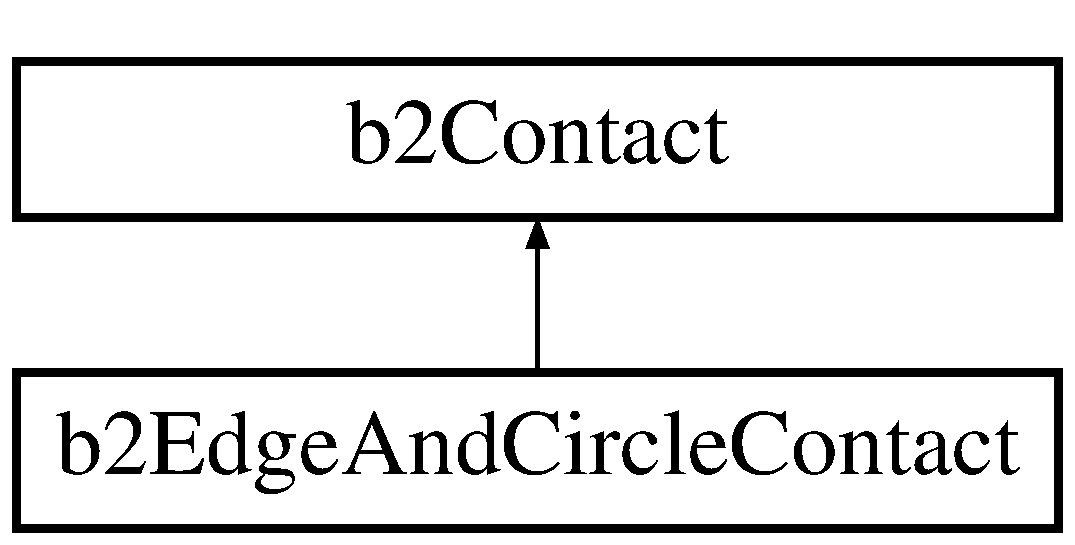
\includegraphics[height=2.000000cm]{classb2EdgeAndCircleContact}
\end{center}
\end{figure}
\subsection*{Public Member Functions}
\begin{DoxyCompactItemize}
\item 
\mbox{\Hypertarget{classb2EdgeAndCircleContact_a9de91d6afe4d2407f679b2ccaded9c02}\label{classb2EdgeAndCircleContact_a9de91d6afe4d2407f679b2ccaded9c02}} 
{\bfseries b2\+Edge\+And\+Circle\+Contact} (\mbox{\hyperlink{classb2Fixture}{b2\+Fixture}} $\ast$fixtureA, \mbox{\hyperlink{classb2Fixture}{b2\+Fixture}} $\ast$fixtureB)
\item 
\mbox{\Hypertarget{classb2EdgeAndCircleContact_aec021f688dcf2b5a2c483edde476d4b6}\label{classb2EdgeAndCircleContact_aec021f688dcf2b5a2c483edde476d4b6}} 
void \mbox{\hyperlink{classb2EdgeAndCircleContact_aec021f688dcf2b5a2c483edde476d4b6}{Evaluate}} (\mbox{\hyperlink{structb2Manifold}{b2\+Manifold}} $\ast$manifold, const \mbox{\hyperlink{structb2Transform}{b2\+Transform}} \&xfA, const \mbox{\hyperlink{structb2Transform}{b2\+Transform}} \&xfB) override
\begin{DoxyCompactList}\small\item\em Evaluate this contact with your own manifold and transforms. \end{DoxyCompactList}\end{DoxyCompactItemize}
\subsection*{Static Public Member Functions}
\begin{DoxyCompactItemize}
\item 
\mbox{\Hypertarget{classb2EdgeAndCircleContact_a1b4a2a1d4098288c84a7778a4949d0f0}\label{classb2EdgeAndCircleContact_a1b4a2a1d4098288c84a7778a4949d0f0}} 
static \mbox{\hyperlink{classb2Contact}{b2\+Contact}} $\ast$ {\bfseries Create} (\mbox{\hyperlink{classb2Fixture}{b2\+Fixture}} $\ast$fixtureA, int32 indexA, \mbox{\hyperlink{classb2Fixture}{b2\+Fixture}} $\ast$fixtureB, int32 indexB, \mbox{\hyperlink{classb2BlockAllocator}{b2\+Block\+Allocator}} $\ast$allocator)
\item 
\mbox{\Hypertarget{classb2EdgeAndCircleContact_a123eeb8144b01fc15c1318eacd0da4ca}\label{classb2EdgeAndCircleContact_a123eeb8144b01fc15c1318eacd0da4ca}} 
static void {\bfseries Destroy} (\mbox{\hyperlink{classb2Contact}{b2\+Contact}} $\ast$contact, \mbox{\hyperlink{classb2BlockAllocator}{b2\+Block\+Allocator}} $\ast$allocator)
\end{DoxyCompactItemize}
\subsection*{Additional Inherited Members}


The documentation for this class was generated from the following files\+:\begin{DoxyCompactItemize}
\item 
Dynamics/\+Contacts/b2\+Edge\+And\+Circle\+Contact.\+h\item 
Dynamics/\+Contacts/b2\+Edge\+And\+Circle\+Contact.\+cpp\end{DoxyCompactItemize}

\hypertarget{classb2EdgeAndPolygonContact}{}\section{b2\+Edge\+And\+Polygon\+Contact Class Reference}
\label{classb2EdgeAndPolygonContact}\index{b2\+Edge\+And\+Polygon\+Contact@{b2\+Edge\+And\+Polygon\+Contact}}
Inheritance diagram for b2\+Edge\+And\+Polygon\+Contact\+:\begin{figure}[H]
\begin{center}
\leavevmode
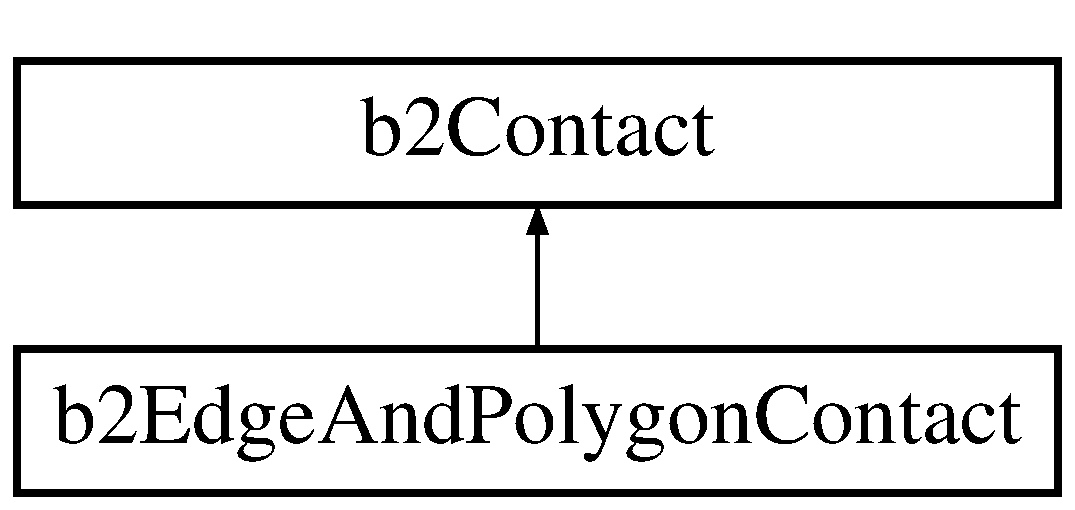
\includegraphics[height=2.000000cm]{classb2EdgeAndPolygonContact}
\end{center}
\end{figure}
\subsection*{Public Member Functions}
\begin{DoxyCompactItemize}
\item 
\mbox{\Hypertarget{classb2EdgeAndPolygonContact_a79d9b012c4a0df7d5c3dcecd33df7d5f}\label{classb2EdgeAndPolygonContact_a79d9b012c4a0df7d5c3dcecd33df7d5f}} 
{\bfseries b2\+Edge\+And\+Polygon\+Contact} (\mbox{\hyperlink{classb2Fixture}{b2\+Fixture}} $\ast$fixtureA, \mbox{\hyperlink{classb2Fixture}{b2\+Fixture}} $\ast$fixtureB)
\item 
\mbox{\Hypertarget{classb2EdgeAndPolygonContact_ae99fba8c1cb7e5d7c11ab78ca80e775d}\label{classb2EdgeAndPolygonContact_ae99fba8c1cb7e5d7c11ab78ca80e775d}} 
void \mbox{\hyperlink{classb2EdgeAndPolygonContact_ae99fba8c1cb7e5d7c11ab78ca80e775d}{Evaluate}} (\mbox{\hyperlink{structb2Manifold}{b2\+Manifold}} $\ast$manifold, const \mbox{\hyperlink{structb2Transform}{b2\+Transform}} \&xfA, const \mbox{\hyperlink{structb2Transform}{b2\+Transform}} \&xfB) override
\begin{DoxyCompactList}\small\item\em Evaluate this contact with your own manifold and transforms. \end{DoxyCompactList}\end{DoxyCompactItemize}
\subsection*{Static Public Member Functions}
\begin{DoxyCompactItemize}
\item 
\mbox{\Hypertarget{classb2EdgeAndPolygonContact_a3a0bcb2327e02bfc2079a734d8e9c8f7}\label{classb2EdgeAndPolygonContact_a3a0bcb2327e02bfc2079a734d8e9c8f7}} 
static \mbox{\hyperlink{classb2Contact}{b2\+Contact}} $\ast$ {\bfseries Create} (\mbox{\hyperlink{classb2Fixture}{b2\+Fixture}} $\ast$fixtureA, int32 indexA, \mbox{\hyperlink{classb2Fixture}{b2\+Fixture}} $\ast$fixtureB, int32 indexB, \mbox{\hyperlink{classb2BlockAllocator}{b2\+Block\+Allocator}} $\ast$allocator)
\item 
\mbox{\Hypertarget{classb2EdgeAndPolygonContact_a83260c190706928518ab1a3040c0c515}\label{classb2EdgeAndPolygonContact_a83260c190706928518ab1a3040c0c515}} 
static void {\bfseries Destroy} (\mbox{\hyperlink{classb2Contact}{b2\+Contact}} $\ast$contact, \mbox{\hyperlink{classb2BlockAllocator}{b2\+Block\+Allocator}} $\ast$allocator)
\end{DoxyCompactItemize}
\subsection*{Additional Inherited Members}


The documentation for this class was generated from the following files\+:\begin{DoxyCompactItemize}
\item 
Dynamics/\+Contacts/b2\+Edge\+And\+Polygon\+Contact.\+h\item 
Dynamics/\+Contacts/b2\+Edge\+And\+Polygon\+Contact.\+cpp\end{DoxyCompactItemize}

\hypertarget{classb2EdgeShape}{}\section{b2\+Edge\+Shape Class Reference}
\label{classb2EdgeShape}\index{b2\+Edge\+Shape@{b2\+Edge\+Shape}}


{\ttfamily \#include $<$b2\+Edge\+Shape.\+h$>$}

Inheritance diagram for b2\+Edge\+Shape\+:\begin{figure}[H]
\begin{center}
\leavevmode
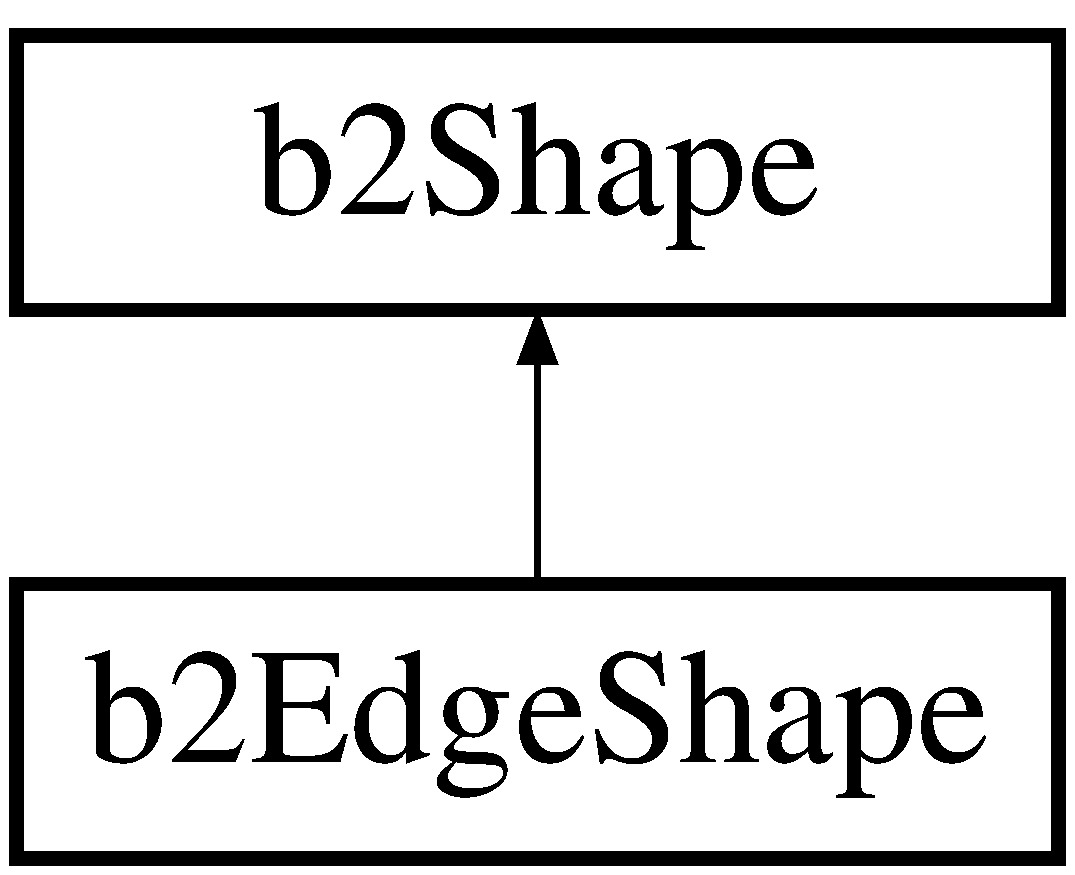
\includegraphics[height=2.000000cm]{classb2EdgeShape}
\end{center}
\end{figure}
\subsection*{Public Member Functions}
\begin{DoxyCompactItemize}
\item 
\mbox{\Hypertarget{classb2EdgeShape_a67dd3b17630a600033cb4380697a4e9d}\label{classb2EdgeShape_a67dd3b17630a600033cb4380697a4e9d}} 
void \mbox{\hyperlink{classb2EdgeShape_a67dd3b17630a600033cb4380697a4e9d}{Set}} (const \mbox{\hyperlink{structb2Vec2}{b2\+Vec2}} \&v1, const \mbox{\hyperlink{structb2Vec2}{b2\+Vec2}} \&v2)
\begin{DoxyCompactList}\small\item\em Set this as an isolated edge. \end{DoxyCompactList}\item 
\mbox{\Hypertarget{classb2EdgeShape_a52ed696717f44ed02b7a88ccf201563c}\label{classb2EdgeShape_a52ed696717f44ed02b7a88ccf201563c}} 
\mbox{\hyperlink{classb2Shape}{b2\+Shape}} $\ast$ \mbox{\hyperlink{classb2EdgeShape_a52ed696717f44ed02b7a88ccf201563c}{Clone}} (\mbox{\hyperlink{classb2BlockAllocator}{b2\+Block\+Allocator}} $\ast$allocator) const override
\begin{DoxyCompactList}\small\item\em Implement \mbox{\hyperlink{classb2Shape}{b2\+Shape}}. \end{DoxyCompactList}\item 
int32 \mbox{\hyperlink{classb2EdgeShape_ae9dcaa2f4b77fcf182d29159658da82a}{Get\+Child\+Count}} () const override
\item 
bool \mbox{\hyperlink{classb2EdgeShape_a15151673cf9ad585779c70363425f470}{Test\+Point}} (const \mbox{\hyperlink{structb2Transform}{b2\+Transform}} \&transform, const \mbox{\hyperlink{structb2Vec2}{b2\+Vec2}} \&p) const override
\item 
\mbox{\Hypertarget{classb2EdgeShape_a192cf10bd556a5a90b29a2bcee2ddd75}\label{classb2EdgeShape_a192cf10bd556a5a90b29a2bcee2ddd75}} 
bool \mbox{\hyperlink{classb2EdgeShape_a192cf10bd556a5a90b29a2bcee2ddd75}{Ray\+Cast}} (\mbox{\hyperlink{structb2RayCastOutput}{b2\+Ray\+Cast\+Output}} $\ast$output, const \mbox{\hyperlink{structb2RayCastInput}{b2\+Ray\+Cast\+Input}} \&input, const \mbox{\hyperlink{structb2Transform}{b2\+Transform}} \&transform, int32 child\+Index) const override
\begin{DoxyCompactList}\small\item\em Implement \mbox{\hyperlink{classb2Shape}{b2\+Shape}}. \end{DoxyCompactList}\item 
void \mbox{\hyperlink{classb2EdgeShape_a238139ae1736b457d77443133ff16854}{Compute\+A\+A\+BB}} (\mbox{\hyperlink{structb2AABB}{b2\+A\+A\+BB}} $\ast$aabb, const \mbox{\hyperlink{structb2Transform}{b2\+Transform}} \&transform, int32 child\+Index) const override
\item 
void \mbox{\hyperlink{classb2EdgeShape_ac738c1e0ab2f4dfbab26e3942efa60af}{Compute\+Mass}} (\mbox{\hyperlink{structb2MassData}{b2\+Mass\+Data}} $\ast$mass\+Data, float32 density) const override
\end{DoxyCompactItemize}
\subsection*{Public Attributes}
\begin{DoxyCompactItemize}
\item 
\mbox{\Hypertarget{classb2EdgeShape_a916cf02a752ff1a70db35b2edaf19bb4}\label{classb2EdgeShape_a916cf02a752ff1a70db35b2edaf19bb4}} 
\mbox{\hyperlink{structb2Vec2}{b2\+Vec2}} \mbox{\hyperlink{classb2EdgeShape_a916cf02a752ff1a70db35b2edaf19bb4}{m\+\_\+vertex1}}
\begin{DoxyCompactList}\small\item\em These are the edge vertices. \end{DoxyCompactList}\item 
\mbox{\Hypertarget{classb2EdgeShape_aa218bfe2bf135e4e94028b29aaa32fce}\label{classb2EdgeShape_aa218bfe2bf135e4e94028b29aaa32fce}} 
\mbox{\hyperlink{structb2Vec2}{b2\+Vec2}} {\bfseries m\+\_\+vertex2}
\item 
\mbox{\Hypertarget{classb2EdgeShape_a907c9829484cc1ba7527ab368e9fdf93}\label{classb2EdgeShape_a907c9829484cc1ba7527ab368e9fdf93}} 
\mbox{\hyperlink{structb2Vec2}{b2\+Vec2}} \mbox{\hyperlink{classb2EdgeShape_a907c9829484cc1ba7527ab368e9fdf93}{m\+\_\+vertex0}}
\begin{DoxyCompactList}\small\item\em Optional adjacent vertices. These are used for smooth collision. \end{DoxyCompactList}\item 
\mbox{\Hypertarget{classb2EdgeShape_a7991fd8b38806a7785748cd991c18452}\label{classb2EdgeShape_a7991fd8b38806a7785748cd991c18452}} 
\mbox{\hyperlink{structb2Vec2}{b2\+Vec2}} {\bfseries m\+\_\+vertex3}
\item 
\mbox{\Hypertarget{classb2EdgeShape_a1d0f39259f0963146b343d6b048f3f8a}\label{classb2EdgeShape_a1d0f39259f0963146b343d6b048f3f8a}} 
bool {\bfseries m\+\_\+has\+Vertex0}
\item 
\mbox{\Hypertarget{classb2EdgeShape_afeb0dfac66fe677ccd765d48610fa56f}\label{classb2EdgeShape_afeb0dfac66fe677ccd765d48610fa56f}} 
bool {\bfseries m\+\_\+has\+Vertex3}
\end{DoxyCompactItemize}
\subsection*{Additional Inherited Members}


\subsection{Detailed Description}
A line segment (edge) shape. These can be connected in chains or loops to other edge shapes. The connectivity information is used to ensure correct contact normals. 

\subsection{Member Function Documentation}
\mbox{\Hypertarget{classb2EdgeShape_a238139ae1736b457d77443133ff16854}\label{classb2EdgeShape_a238139ae1736b457d77443133ff16854}} 
\index{b2\+Edge\+Shape@{b2\+Edge\+Shape}!Compute\+A\+A\+BB@{Compute\+A\+A\+BB}}
\index{Compute\+A\+A\+BB@{Compute\+A\+A\+BB}!b2\+Edge\+Shape@{b2\+Edge\+Shape}}
\subsubsection{\texorpdfstring{Compute\+A\+A\+B\+B()}{ComputeAABB()}}
{\footnotesize\ttfamily void b2\+Edge\+Shape\+::\+Compute\+A\+A\+BB (\begin{DoxyParamCaption}\item[{\mbox{\hyperlink{structb2AABB}{b2\+A\+A\+BB}} $\ast$}]{aabb,  }\item[{const \mbox{\hyperlink{structb2Transform}{b2\+Transform}} \&}]{transform,  }\item[{int32}]{child\+Index }\end{DoxyParamCaption}) const\hspace{0.3cm}{\ttfamily [override]}, {\ttfamily [virtual]}}

\begin{DoxySeeAlso}{See also}
\mbox{\hyperlink{classb2Shape_a88e9807fab0c8ca9a98d8926e50a1411}{b2\+Shape\+::\+Compute\+A\+A\+BB}} 
\end{DoxySeeAlso}


Implements \mbox{\hyperlink{classb2Shape_a88e9807fab0c8ca9a98d8926e50a1411}{b2\+Shape}}.

\mbox{\Hypertarget{classb2EdgeShape_ac738c1e0ab2f4dfbab26e3942efa60af}\label{classb2EdgeShape_ac738c1e0ab2f4dfbab26e3942efa60af}} 
\index{b2\+Edge\+Shape@{b2\+Edge\+Shape}!Compute\+Mass@{Compute\+Mass}}
\index{Compute\+Mass@{Compute\+Mass}!b2\+Edge\+Shape@{b2\+Edge\+Shape}}
\subsubsection{\texorpdfstring{Compute\+Mass()}{ComputeMass()}}
{\footnotesize\ttfamily void b2\+Edge\+Shape\+::\+Compute\+Mass (\begin{DoxyParamCaption}\item[{\mbox{\hyperlink{structb2MassData}{b2\+Mass\+Data}} $\ast$}]{mass\+Data,  }\item[{float32}]{density }\end{DoxyParamCaption}) const\hspace{0.3cm}{\ttfamily [override]}, {\ttfamily [virtual]}}

\begin{DoxySeeAlso}{See also}
\mbox{\hyperlink{classb2Shape_a61b365526241b47f124789b0309cac69}{b2\+Shape\+::\+Compute\+Mass}} 
\end{DoxySeeAlso}


Implements \mbox{\hyperlink{classb2Shape_a61b365526241b47f124789b0309cac69}{b2\+Shape}}.

\mbox{\Hypertarget{classb2EdgeShape_ae9dcaa2f4b77fcf182d29159658da82a}\label{classb2EdgeShape_ae9dcaa2f4b77fcf182d29159658da82a}} 
\index{b2\+Edge\+Shape@{b2\+Edge\+Shape}!Get\+Child\+Count@{Get\+Child\+Count}}
\index{Get\+Child\+Count@{Get\+Child\+Count}!b2\+Edge\+Shape@{b2\+Edge\+Shape}}
\subsubsection{\texorpdfstring{Get\+Child\+Count()}{GetChildCount()}}
{\footnotesize\ttfamily int32 b2\+Edge\+Shape\+::\+Get\+Child\+Count (\begin{DoxyParamCaption}{ }\end{DoxyParamCaption}) const\hspace{0.3cm}{\ttfamily [override]}, {\ttfamily [virtual]}}

\begin{DoxySeeAlso}{See also}
\mbox{\hyperlink{classb2Shape_a05a3c445017d96df9238ceefe6ce37ab}{b2\+Shape\+::\+Get\+Child\+Count}} 
\end{DoxySeeAlso}


Implements \mbox{\hyperlink{classb2Shape_a05a3c445017d96df9238ceefe6ce37ab}{b2\+Shape}}.

\mbox{\Hypertarget{classb2EdgeShape_a15151673cf9ad585779c70363425f470}\label{classb2EdgeShape_a15151673cf9ad585779c70363425f470}} 
\index{b2\+Edge\+Shape@{b2\+Edge\+Shape}!Test\+Point@{Test\+Point}}
\index{Test\+Point@{Test\+Point}!b2\+Edge\+Shape@{b2\+Edge\+Shape}}
\subsubsection{\texorpdfstring{Test\+Point()}{TestPoint()}}
{\footnotesize\ttfamily bool b2\+Edge\+Shape\+::\+Test\+Point (\begin{DoxyParamCaption}\item[{const \mbox{\hyperlink{structb2Transform}{b2\+Transform}} \&}]{transform,  }\item[{const \mbox{\hyperlink{structb2Vec2}{b2\+Vec2}} \&}]{p }\end{DoxyParamCaption}) const\hspace{0.3cm}{\ttfamily [override]}, {\ttfamily [virtual]}}

\begin{DoxySeeAlso}{See also}
\mbox{\hyperlink{classb2Shape_a6ac968e403e2d93e8ae46d728a2e50fa}{b2\+Shape\+::\+Test\+Point}} 
\end{DoxySeeAlso}


Implements \mbox{\hyperlink{classb2Shape_a6ac968e403e2d93e8ae46d728a2e50fa}{b2\+Shape}}.



The documentation for this class was generated from the following files\+:\begin{DoxyCompactItemize}
\item 
Collision/\+Shapes/b2\+Edge\+Shape.\+h\item 
Collision/\+Shapes/b2\+Edge\+Shape.\+cpp\end{DoxyCompactItemize}

\hypertarget{structb2EPAxis}{}\section{b2\+E\+P\+Axis Struct Reference}
\label{structb2EPAxis}\index{b2\+E\+P\+Axis@{b2\+E\+P\+Axis}}
\subsection*{Public Types}
\begin{DoxyCompactItemize}
\item 
\mbox{\Hypertarget{structb2EPAxis_a1a2feab0d321a5cd20677c92cbfd6f3c}\label{structb2EPAxis_a1a2feab0d321a5cd20677c92cbfd6f3c}} 
enum {\bfseries Type} \{ {\bfseries e\+\_\+unknown}, 
{\bfseries e\+\_\+edgeA}, 
{\bfseries e\+\_\+edgeB}
 \}
\end{DoxyCompactItemize}
\subsection*{Public Attributes}
\begin{DoxyCompactItemize}
\item 
\mbox{\Hypertarget{structb2EPAxis_a336d3ba4b4ed020a1f6c4c0f70098e39}\label{structb2EPAxis_a336d3ba4b4ed020a1f6c4c0f70098e39}} 
Type {\bfseries type}
\item 
\mbox{\Hypertarget{structb2EPAxis_a8e530d411d98e7ab8112c4022f5f65e4}\label{structb2EPAxis_a8e530d411d98e7ab8112c4022f5f65e4}} 
int32 {\bfseries index}
\item 
\mbox{\Hypertarget{structb2EPAxis_acfd60cfd1f1ad4c448bd0260117ef6fc}\label{structb2EPAxis_acfd60cfd1f1ad4c448bd0260117ef6fc}} 
float32 {\bfseries separation}
\end{DoxyCompactItemize}


The documentation for this struct was generated from the following file\+:\begin{DoxyCompactItemize}
\item 
Collision/b2\+Collide\+Edge.\+cpp\end{DoxyCompactItemize}

\hypertarget{structb2EPCollider}{}\section{b2\+E\+P\+Collider Struct Reference}
\label{structb2EPCollider}\index{b2\+E\+P\+Collider@{b2\+E\+P\+Collider}}
\subsection*{Public Types}
\begin{DoxyCompactItemize}
\item 
\mbox{\Hypertarget{structb2EPCollider_aa50efcaf41cf85e167d0244f5d6f00e8}\label{structb2EPCollider_aa50efcaf41cf85e167d0244f5d6f00e8}} 
enum {\bfseries Vertex\+Type} \{ {\bfseries e\+\_\+isolated}, 
{\bfseries e\+\_\+concave}, 
{\bfseries e\+\_\+convex}
 \}
\end{DoxyCompactItemize}
\subsection*{Public Member Functions}
\begin{DoxyCompactItemize}
\item 
\mbox{\Hypertarget{structb2EPCollider_a22f13698b4adde74b9bdb705f59f9778}\label{structb2EPCollider_a22f13698b4adde74b9bdb705f59f9778}} 
void {\bfseries Collide} (\mbox{\hyperlink{structb2Manifold}{b2\+Manifold}} $\ast$manifold, const \mbox{\hyperlink{classb2EdgeShape}{b2\+Edge\+Shape}} $\ast$edgeA, const \mbox{\hyperlink{structb2Transform}{b2\+Transform}} \&xfA, const \mbox{\hyperlink{classb2PolygonShape}{b2\+Polygon\+Shape}} $\ast$polygonB, const \mbox{\hyperlink{structb2Transform}{b2\+Transform}} \&xfB)
\item 
\mbox{\Hypertarget{structb2EPCollider_a105a28c48afe6dc4158e6d5d303bf5e1}\label{structb2EPCollider_a105a28c48afe6dc4158e6d5d303bf5e1}} 
\mbox{\hyperlink{structb2EPAxis}{b2\+E\+P\+Axis}} {\bfseries Compute\+Edge\+Separation} ()
\item 
\mbox{\Hypertarget{structb2EPCollider_a46c340d43b25b776db8356c5b0249002}\label{structb2EPCollider_a46c340d43b25b776db8356c5b0249002}} 
\mbox{\hyperlink{structb2EPAxis}{b2\+E\+P\+Axis}} {\bfseries Compute\+Polygon\+Separation} ()
\end{DoxyCompactItemize}
\subsection*{Public Attributes}
\begin{DoxyCompactItemize}
\item 
\mbox{\Hypertarget{structb2EPCollider_ae01f6c0b04cc1b24af41c5772fd1d96a}\label{structb2EPCollider_ae01f6c0b04cc1b24af41c5772fd1d96a}} 
\mbox{\hyperlink{structb2TempPolygon}{b2\+Temp\+Polygon}} {\bfseries m\+\_\+polygonB}
\item 
\mbox{\Hypertarget{structb2EPCollider_a096b61a983a24fa26ee3089b4ec59ab8}\label{structb2EPCollider_a096b61a983a24fa26ee3089b4ec59ab8}} 
\mbox{\hyperlink{structb2Transform}{b2\+Transform}} {\bfseries m\+\_\+xf}
\item 
\mbox{\Hypertarget{structb2EPCollider_a8635888e0c36a76b08b0b0ec7cf6e6e9}\label{structb2EPCollider_a8635888e0c36a76b08b0b0ec7cf6e6e9}} 
\mbox{\hyperlink{structb2Vec2}{b2\+Vec2}} {\bfseries m\+\_\+centroidB}
\item 
\mbox{\Hypertarget{structb2EPCollider_a309b7ea4262921a25ba1f14b002375ee}\label{structb2EPCollider_a309b7ea4262921a25ba1f14b002375ee}} 
\mbox{\hyperlink{structb2Vec2}{b2\+Vec2}} {\bfseries m\+\_\+v0}
\item 
\mbox{\Hypertarget{structb2EPCollider_a710cbfefe79857ef97363a932be23048}\label{structb2EPCollider_a710cbfefe79857ef97363a932be23048}} 
\mbox{\hyperlink{structb2Vec2}{b2\+Vec2}} {\bfseries m\+\_\+v1}
\item 
\mbox{\Hypertarget{structb2EPCollider_a9888184f541622203bed3087c896eb0e}\label{structb2EPCollider_a9888184f541622203bed3087c896eb0e}} 
\mbox{\hyperlink{structb2Vec2}{b2\+Vec2}} {\bfseries m\+\_\+v2}
\item 
\mbox{\Hypertarget{structb2EPCollider_a4a866752c895e5239e251d9903d281f4}\label{structb2EPCollider_a4a866752c895e5239e251d9903d281f4}} 
\mbox{\hyperlink{structb2Vec2}{b2\+Vec2}} {\bfseries m\+\_\+v3}
\item 
\mbox{\Hypertarget{structb2EPCollider_ac2c16435adf5cfa90817399dbfe9ce89}\label{structb2EPCollider_ac2c16435adf5cfa90817399dbfe9ce89}} 
\mbox{\hyperlink{structb2Vec2}{b2\+Vec2}} {\bfseries m\+\_\+normal0}
\item 
\mbox{\Hypertarget{structb2EPCollider_abe08dfafd360c41c5ae80a30840b7d63}\label{structb2EPCollider_abe08dfafd360c41c5ae80a30840b7d63}} 
\mbox{\hyperlink{structb2Vec2}{b2\+Vec2}} {\bfseries m\+\_\+normal1}
\item 
\mbox{\Hypertarget{structb2EPCollider_aaec4f7ff250911272c054e3bfe65e08b}\label{structb2EPCollider_aaec4f7ff250911272c054e3bfe65e08b}} 
\mbox{\hyperlink{structb2Vec2}{b2\+Vec2}} {\bfseries m\+\_\+normal2}
\item 
\mbox{\Hypertarget{structb2EPCollider_a67ff23f9fada3a733928380da8653348}\label{structb2EPCollider_a67ff23f9fada3a733928380da8653348}} 
\mbox{\hyperlink{structb2Vec2}{b2\+Vec2}} {\bfseries m\+\_\+normal}
\item 
\mbox{\Hypertarget{structb2EPCollider_ad2541e4c9358d5ffcaca19b25836392b}\label{structb2EPCollider_ad2541e4c9358d5ffcaca19b25836392b}} 
Vertex\+Type {\bfseries m\+\_\+type1}
\item 
\mbox{\Hypertarget{structb2EPCollider_a71889f34bef412e3cbfbbab605210b7e}\label{structb2EPCollider_a71889f34bef412e3cbfbbab605210b7e}} 
Vertex\+Type {\bfseries m\+\_\+type2}
\item 
\mbox{\Hypertarget{structb2EPCollider_a6b48818ac312de825aaf55b46aceea1e}\label{structb2EPCollider_a6b48818ac312de825aaf55b46aceea1e}} 
\mbox{\hyperlink{structb2Vec2}{b2\+Vec2}} {\bfseries m\+\_\+lower\+Limit}
\item 
\mbox{\Hypertarget{structb2EPCollider_a5da77944d10d87ca7222e3d8d00ac205}\label{structb2EPCollider_a5da77944d10d87ca7222e3d8d00ac205}} 
\mbox{\hyperlink{structb2Vec2}{b2\+Vec2}} {\bfseries m\+\_\+upper\+Limit}
\item 
\mbox{\Hypertarget{structb2EPCollider_a1efd359a8c17680bbdef093dd07fbb9d}\label{structb2EPCollider_a1efd359a8c17680bbdef093dd07fbb9d}} 
float32 {\bfseries m\+\_\+radius}
\item 
\mbox{\Hypertarget{structb2EPCollider_aa9443e27e043bf80916992ca96bdedd2}\label{structb2EPCollider_aa9443e27e043bf80916992ca96bdedd2}} 
bool {\bfseries m\+\_\+front}
\end{DoxyCompactItemize}


The documentation for this struct was generated from the following file\+:\begin{DoxyCompactItemize}
\item 
Collision/b2\+Collide\+Edge.\+cpp\end{DoxyCompactItemize}

\hypertarget{structb2Filter}{}\section{b2\+Filter Struct Reference}
\label{structb2Filter}\index{b2\+Filter@{b2\+Filter}}


This holds contact filtering data.  




{\ttfamily \#include $<$b2\+Fixture.\+h$>$}

\subsection*{Public Attributes}
\begin{DoxyCompactItemize}
\item 
\mbox{\Hypertarget{structb2Filter_a368907397168d39af8b4fc5201d50bba}\label{structb2Filter_a368907397168d39af8b4fc5201d50bba}} 
uint16 \mbox{\hyperlink{structb2Filter_a368907397168d39af8b4fc5201d50bba}{category\+Bits}}
\begin{DoxyCompactList}\small\item\em The collision category bits. Normally you would just set one bit. \end{DoxyCompactList}\item 
uint16 \mbox{\hyperlink{structb2Filter_a533cccf85e3ba3d9e3700d73b819f6e2}{mask\+Bits}}
\item 
int16 \mbox{\hyperlink{structb2Filter_a572a8f4a1672f6d5d71123a35e872950}{group\+Index}}
\end{DoxyCompactItemize}


\subsection{Detailed Description}
This holds contact filtering data. 

\subsection{Member Data Documentation}
\mbox{\Hypertarget{structb2Filter_a572a8f4a1672f6d5d71123a35e872950}\label{structb2Filter_a572a8f4a1672f6d5d71123a35e872950}} 
\index{b2\+Filter@{b2\+Filter}!group\+Index@{group\+Index}}
\index{group\+Index@{group\+Index}!b2\+Filter@{b2\+Filter}}
\subsubsection{\texorpdfstring{group\+Index}{groupIndex}}
{\footnotesize\ttfamily int16 b2\+Filter\+::group\+Index}

Collision groups allow a certain group of objects to never collide (negative) or always collide (positive). Zero means no collision group. Non-\/zero group filtering always wins against the mask bits. \mbox{\Hypertarget{structb2Filter_a533cccf85e3ba3d9e3700d73b819f6e2}\label{structb2Filter_a533cccf85e3ba3d9e3700d73b819f6e2}} 
\index{b2\+Filter@{b2\+Filter}!mask\+Bits@{mask\+Bits}}
\index{mask\+Bits@{mask\+Bits}!b2\+Filter@{b2\+Filter}}
\subsubsection{\texorpdfstring{mask\+Bits}{maskBits}}
{\footnotesize\ttfamily uint16 b2\+Filter\+::mask\+Bits}

The collision mask bits. This states the categories that this shape would accept for collision. 

The documentation for this struct was generated from the following file\+:\begin{DoxyCompactItemize}
\item 
Dynamics/b2\+Fixture.\+h\end{DoxyCompactItemize}

\hypertarget{classb2Fixture}{}\section{b2\+Fixture Class Reference}
\label{classb2Fixture}\index{b2\+Fixture@{b2\+Fixture}}


{\ttfamily \#include $<$b2\+Fixture.\+h$>$}

\subsection*{Public Member Functions}
\begin{DoxyCompactItemize}
\item 
b2\+Shape\+::\+Type \mbox{\hyperlink{classb2Fixture_a7a566c1e3b768f6a72ebc3b758aad70e}{Get\+Type}} () const
\item 
\mbox{\hyperlink{classb2Shape}{b2\+Shape}} $\ast$ \mbox{\hyperlink{classb2Fixture_aaa2b73fa212fa53b1c800cccd7a1d31e}{Get\+Shape}} ()
\item 
\mbox{\Hypertarget{classb2Fixture_a783f8bcb19eee659686284872e70f383}\label{classb2Fixture_a783f8bcb19eee659686284872e70f383}} 
const \mbox{\hyperlink{classb2Shape}{b2\+Shape}} $\ast$ {\bfseries Get\+Shape} () const
\item 
\mbox{\Hypertarget{classb2Fixture_a6198a81dcee0fe814d730383ebfa7038}\label{classb2Fixture_a6198a81dcee0fe814d730383ebfa7038}} 
void \mbox{\hyperlink{classb2Fixture_a6198a81dcee0fe814d730383ebfa7038}{Set\+Sensor}} (bool sensor)
\begin{DoxyCompactList}\small\item\em Set if this fixture is a sensor. \end{DoxyCompactList}\item 
bool \mbox{\hyperlink{classb2Fixture_aedd23d27ff7ce2d53b6c5b7a878a35d3}{Is\+Sensor}} () const
\item 
void \mbox{\hyperlink{classb2Fixture_a2c5e0d12c174927a4ad550459be334ad}{Set\+Filter\+Data}} (const \mbox{\hyperlink{structb2Filter}{b2\+Filter}} \&filter)
\item 
\mbox{\Hypertarget{classb2Fixture_ad956250d9f684a407992ec178320127e}\label{classb2Fixture_ad956250d9f684a407992ec178320127e}} 
const \mbox{\hyperlink{structb2Filter}{b2\+Filter}} \& \mbox{\hyperlink{classb2Fixture_ad956250d9f684a407992ec178320127e}{Get\+Filter\+Data}} () const
\begin{DoxyCompactList}\small\item\em Get the contact filtering data. \end{DoxyCompactList}\item 
\mbox{\Hypertarget{classb2Fixture_a45d3320f94811d67383c48466165fa26}\label{classb2Fixture_a45d3320f94811d67383c48466165fa26}} 
void \mbox{\hyperlink{classb2Fixture_a45d3320f94811d67383c48466165fa26}{Refilter}} ()
\begin{DoxyCompactList}\small\item\em Call this if you want to establish collision that was previously disabled by \mbox{\hyperlink{classb2ContactFilter_aac8f6155d1f577d125db587f5269289b}{b2\+Contact\+Filter\+::\+Should\+Collide}}. \end{DoxyCompactList}\item 
\mbox{\hyperlink{classb2Body}{b2\+Body}} $\ast$ \mbox{\hyperlink{classb2Fixture_a9d6536ef274d768e86ab0a8330921535}{Get\+Body}} ()
\item 
\mbox{\Hypertarget{classb2Fixture_ae9cabf82e360f92e8fcb36b1923ab991}\label{classb2Fixture_ae9cabf82e360f92e8fcb36b1923ab991}} 
const \mbox{\hyperlink{classb2Body}{b2\+Body}} $\ast$ {\bfseries Get\+Body} () const
\item 
\mbox{\hyperlink{classb2Fixture}{b2\+Fixture}} $\ast$ \mbox{\hyperlink{classb2Fixture_a0241952461f6f1a04a3c850306390fd2}{Get\+Next}} ()
\item 
\mbox{\Hypertarget{classb2Fixture_a6b474fa22b49de3dbe446a67f021beb2}\label{classb2Fixture_a6b474fa22b49de3dbe446a67f021beb2}} 
const \mbox{\hyperlink{classb2Fixture}{b2\+Fixture}} $\ast$ {\bfseries Get\+Next} () const
\item 
void $\ast$ \mbox{\hyperlink{classb2Fixture_ae2a865ed59ffe9b1cb89f577052f4d50}{Get\+User\+Data}} () const
\item 
\mbox{\Hypertarget{classb2Fixture_a3db7f89ef4493247d922fe3d96351ad9}\label{classb2Fixture_a3db7f89ef4493247d922fe3d96351ad9}} 
void \mbox{\hyperlink{classb2Fixture_a3db7f89ef4493247d922fe3d96351ad9}{Set\+User\+Data}} (void $\ast$data)
\begin{DoxyCompactList}\small\item\em Set the user data. Use this to store your application specific data. \end{DoxyCompactList}\item 
bool \mbox{\hyperlink{classb2Fixture_aa56d3ca04a5d0478c6477876cd480cc6}{Test\+Point}} (const \mbox{\hyperlink{structb2Vec2}{b2\+Vec2}} \&p) const
\item 
bool \mbox{\hyperlink{classb2Fixture_aaaafd69aa3e1a922acc4b9d7fb49170a}{Ray\+Cast}} (\mbox{\hyperlink{structb2RayCastOutput}{b2\+Ray\+Cast\+Output}} $\ast$output, const \mbox{\hyperlink{structb2RayCastInput}{b2\+Ray\+Cast\+Input}} \&input, int32 child\+Index) const
\item 
void \mbox{\hyperlink{classb2Fixture_a4532a12e848c5ceb5a3b94cf45b7cbad}{Get\+Mass\+Data}} (\mbox{\hyperlink{structb2MassData}{b2\+Mass\+Data}} $\ast$mass\+Data) const
\item 
void \mbox{\hyperlink{classb2Fixture_ad4e1d9323103975c8931d022b952d04a}{Set\+Density}} (float32 density)
\item 
\mbox{\Hypertarget{classb2Fixture_a228861bb1b1d7b2fb6e091401340784e}\label{classb2Fixture_a228861bb1b1d7b2fb6e091401340784e}} 
float32 \mbox{\hyperlink{classb2Fixture_a228861bb1b1d7b2fb6e091401340784e}{Get\+Density}} () const
\begin{DoxyCompactList}\small\item\em Get the density of this fixture. \end{DoxyCompactList}\item 
\mbox{\Hypertarget{classb2Fixture_a2853d799f299cb1ce76e48261d42a5ad}\label{classb2Fixture_a2853d799f299cb1ce76e48261d42a5ad}} 
float32 \mbox{\hyperlink{classb2Fixture_a2853d799f299cb1ce76e48261d42a5ad}{Get\+Friction}} () const
\begin{DoxyCompactList}\small\item\em Get the coefficient of friction. \end{DoxyCompactList}\item 
void \mbox{\hyperlink{classb2Fixture_ad0cd91eef5858c8ef1d6b62cc2a34ea2}{Set\+Friction}} (float32 friction)
\item 
\mbox{\Hypertarget{classb2Fixture_ac30becb6f936a9cc825952ca2b40aa14}\label{classb2Fixture_ac30becb6f936a9cc825952ca2b40aa14}} 
float32 \mbox{\hyperlink{classb2Fixture_ac30becb6f936a9cc825952ca2b40aa14}{Get\+Restitution}} () const
\begin{DoxyCompactList}\small\item\em Get the coefficient of restitution. \end{DoxyCompactList}\item 
void \mbox{\hyperlink{classb2Fixture_a19c507332e4f7bd04a05f00426f11ee4}{Set\+Restitution}} (float32 restitution)
\item 
const \mbox{\hyperlink{structb2AABB}{b2\+A\+A\+BB}} \& \mbox{\hyperlink{classb2Fixture_a158574dc389fec83a05b09ab715c4474}{Get\+A\+A\+BB}} (int32 child\+Index) const
\item 
\mbox{\Hypertarget{classb2Fixture_a57485e73a2063060e320c7176676cd5e}\label{classb2Fixture_a57485e73a2063060e320c7176676cd5e}} 
void \mbox{\hyperlink{classb2Fixture_a57485e73a2063060e320c7176676cd5e}{Dump}} (int32 body\+Index)
\begin{DoxyCompactList}\small\item\em Dump this fixture to the log file. \end{DoxyCompactList}\end{DoxyCompactItemize}
\subsection*{Protected Member Functions}
\begin{DoxyCompactItemize}
\item 
\mbox{\Hypertarget{classb2Fixture_a1f465f3656f098eebfcbc6edf7a9239a}\label{classb2Fixture_a1f465f3656f098eebfcbc6edf7a9239a}} 
void {\bfseries Create} (\mbox{\hyperlink{classb2BlockAllocator}{b2\+Block\+Allocator}} $\ast$allocator, \mbox{\hyperlink{classb2Body}{b2\+Body}} $\ast$body, const \mbox{\hyperlink{structb2FixtureDef}{b2\+Fixture\+Def}} $\ast$def)
\item 
\mbox{\Hypertarget{classb2Fixture_a279301181668f724c027020a654efe42}\label{classb2Fixture_a279301181668f724c027020a654efe42}} 
void {\bfseries Destroy} (\mbox{\hyperlink{classb2BlockAllocator}{b2\+Block\+Allocator}} $\ast$allocator)
\item 
\mbox{\Hypertarget{classb2Fixture_a670f1f687521666da6e92885754970b7}\label{classb2Fixture_a670f1f687521666da6e92885754970b7}} 
void {\bfseries Create\+Proxies} (\mbox{\hyperlink{classb2BroadPhase}{b2\+Broad\+Phase}} $\ast$broad\+Phase, const \mbox{\hyperlink{structb2Transform}{b2\+Transform}} \&xf)
\item 
\mbox{\Hypertarget{classb2Fixture_a1def068c9ce09e2ebcccc556951b7979}\label{classb2Fixture_a1def068c9ce09e2ebcccc556951b7979}} 
void {\bfseries Destroy\+Proxies} (\mbox{\hyperlink{classb2BroadPhase}{b2\+Broad\+Phase}} $\ast$broad\+Phase)
\item 
\mbox{\Hypertarget{classb2Fixture_ac8fd15bfd9a3a7ba05f3831e6f598908}\label{classb2Fixture_ac8fd15bfd9a3a7ba05f3831e6f598908}} 
void {\bfseries Synchronize} (\mbox{\hyperlink{classb2BroadPhase}{b2\+Broad\+Phase}} $\ast$broad\+Phase, const \mbox{\hyperlink{structb2Transform}{b2\+Transform}} \&xf1, const \mbox{\hyperlink{structb2Transform}{b2\+Transform}} \&xf2)
\end{DoxyCompactItemize}
\subsection*{Protected Attributes}
\begin{DoxyCompactItemize}
\item 
\mbox{\Hypertarget{classb2Fixture_ab8c388182fc7d58d930f6b0aa21d5c60}\label{classb2Fixture_ab8c388182fc7d58d930f6b0aa21d5c60}} 
float32 {\bfseries m\+\_\+density}
\item 
\mbox{\Hypertarget{classb2Fixture_ac5c9fbdf66290e2608db1ffcea2316b0}\label{classb2Fixture_ac5c9fbdf66290e2608db1ffcea2316b0}} 
\mbox{\hyperlink{classb2Fixture}{b2\+Fixture}} $\ast$ {\bfseries m\+\_\+next}
\item 
\mbox{\Hypertarget{classb2Fixture_a480026124a6b7e88f2ed89832a08d191}\label{classb2Fixture_a480026124a6b7e88f2ed89832a08d191}} 
\mbox{\hyperlink{classb2Body}{b2\+Body}} $\ast$ {\bfseries m\+\_\+body}
\item 
\mbox{\Hypertarget{classb2Fixture_a54fa48dfc8b70a435c8f17f8b7720828}\label{classb2Fixture_a54fa48dfc8b70a435c8f17f8b7720828}} 
\mbox{\hyperlink{classb2Shape}{b2\+Shape}} $\ast$ {\bfseries m\+\_\+shape}
\item 
\mbox{\Hypertarget{classb2Fixture_a314118ee973ebd14e083553fed1e0212}\label{classb2Fixture_a314118ee973ebd14e083553fed1e0212}} 
float32 {\bfseries m\+\_\+friction}
\item 
\mbox{\Hypertarget{classb2Fixture_a343a35683ce4a79d2151761611027d66}\label{classb2Fixture_a343a35683ce4a79d2151761611027d66}} 
float32 {\bfseries m\+\_\+restitution}
\item 
\mbox{\Hypertarget{classb2Fixture_a0056031e2b2b53e6a4c0ef7a0c87821a}\label{classb2Fixture_a0056031e2b2b53e6a4c0ef7a0c87821a}} 
\mbox{\hyperlink{structb2FixtureProxy}{b2\+Fixture\+Proxy}} $\ast$ {\bfseries m\+\_\+proxies}
\item 
\mbox{\Hypertarget{classb2Fixture_aae71b4a0071346aba2eb6f4a764785a4}\label{classb2Fixture_aae71b4a0071346aba2eb6f4a764785a4}} 
int32 {\bfseries m\+\_\+proxy\+Count}
\item 
\mbox{\Hypertarget{classb2Fixture_a33b66959856506a6d27b32dad0e284c7}\label{classb2Fixture_a33b66959856506a6d27b32dad0e284c7}} 
\mbox{\hyperlink{structb2Filter}{b2\+Filter}} {\bfseries m\+\_\+filter}
\item 
\mbox{\Hypertarget{classb2Fixture_a4b6b47a8de6d37acf9b980b33b22f634}\label{classb2Fixture_a4b6b47a8de6d37acf9b980b33b22f634}} 
bool {\bfseries m\+\_\+is\+Sensor}
\item 
\mbox{\Hypertarget{classb2Fixture_a60191e5c76bfd115e6c38d78b6cffd8b}\label{classb2Fixture_a60191e5c76bfd115e6c38d78b6cffd8b}} 
void $\ast$ {\bfseries m\+\_\+user\+Data}
\end{DoxyCompactItemize}
\subsection*{Friends}
\begin{DoxyCompactItemize}
\item 
\mbox{\Hypertarget{classb2Fixture_a010ab52de250e5fe30a45d642f46405b}\label{classb2Fixture_a010ab52de250e5fe30a45d642f46405b}} 
class {\bfseries b2\+Body}
\item 
\mbox{\Hypertarget{classb2Fixture_a4bd536c5a7c0587913765bbc2693ceea}\label{classb2Fixture_a4bd536c5a7c0587913765bbc2693ceea}} 
class {\bfseries b2\+World}
\item 
\mbox{\Hypertarget{classb2Fixture_a6c4ac5df27ec498dd9e4281352b7a789}\label{classb2Fixture_a6c4ac5df27ec498dd9e4281352b7a789}} 
class {\bfseries b2\+Contact}
\item 
\mbox{\Hypertarget{classb2Fixture_aece264d42f69aed410f5eb3beba6ddf2}\label{classb2Fixture_aece264d42f69aed410f5eb3beba6ddf2}} 
class {\bfseries b2\+Contact\+Manager}
\end{DoxyCompactItemize}


\subsection{Detailed Description}
A fixture is used to attach a shape to a body for collision detection. A fixture inherits its transform from its parent. Fixtures hold additional non-\/geometric data such as friction, collision filters, etc. Fixtures are created via \mbox{\hyperlink{classb2Body_aa4892301e9b9d62ede5e93dad1743894}{b2\+Body\+::\+Create\+Fixture}}. \begin{DoxyWarning}{Warning}
you cannot reuse fixtures. 
\end{DoxyWarning}


\subsection{Member Function Documentation}
\mbox{\Hypertarget{classb2Fixture_a158574dc389fec83a05b09ab715c4474}\label{classb2Fixture_a158574dc389fec83a05b09ab715c4474}} 
\index{b2\+Fixture@{b2\+Fixture}!Get\+A\+A\+BB@{Get\+A\+A\+BB}}
\index{Get\+A\+A\+BB@{Get\+A\+A\+BB}!b2\+Fixture@{b2\+Fixture}}
\subsubsection{\texorpdfstring{Get\+A\+A\+B\+B()}{GetAABB()}}
{\footnotesize\ttfamily const \mbox{\hyperlink{structb2AABB}{b2\+A\+A\+BB}} \& b2\+Fixture\+::\+Get\+A\+A\+BB (\begin{DoxyParamCaption}\item[{int32}]{child\+Index }\end{DoxyParamCaption}) const\hspace{0.3cm}{\ttfamily [inline]}}

Get the fixture\textquotesingle{}s A\+A\+BB. This A\+A\+BB may be enlarge and/or stale. If you need a more accurate A\+A\+BB, compute it using the shape and the body transform. \mbox{\Hypertarget{classb2Fixture_a9d6536ef274d768e86ab0a8330921535}\label{classb2Fixture_a9d6536ef274d768e86ab0a8330921535}} 
\index{b2\+Fixture@{b2\+Fixture}!Get\+Body@{Get\+Body}}
\index{Get\+Body@{Get\+Body}!b2\+Fixture@{b2\+Fixture}}
\subsubsection{\texorpdfstring{Get\+Body()}{GetBody()}}
{\footnotesize\ttfamily \mbox{\hyperlink{classb2Body}{b2\+Body}} $\ast$ b2\+Fixture\+::\+Get\+Body (\begin{DoxyParamCaption}{ }\end{DoxyParamCaption})\hspace{0.3cm}{\ttfamily [inline]}}

Get the parent body of this fixture. This is nullptr if the fixture is not attached. \begin{DoxyReturn}{Returns}
the parent body. 
\end{DoxyReturn}
\mbox{\Hypertarget{classb2Fixture_a4532a12e848c5ceb5a3b94cf45b7cbad}\label{classb2Fixture_a4532a12e848c5ceb5a3b94cf45b7cbad}} 
\index{b2\+Fixture@{b2\+Fixture}!Get\+Mass\+Data@{Get\+Mass\+Data}}
\index{Get\+Mass\+Data@{Get\+Mass\+Data}!b2\+Fixture@{b2\+Fixture}}
\subsubsection{\texorpdfstring{Get\+Mass\+Data()}{GetMassData()}}
{\footnotesize\ttfamily void b2\+Fixture\+::\+Get\+Mass\+Data (\begin{DoxyParamCaption}\item[{\mbox{\hyperlink{structb2MassData}{b2\+Mass\+Data}} $\ast$}]{mass\+Data }\end{DoxyParamCaption}) const\hspace{0.3cm}{\ttfamily [inline]}}

Get the mass data for this fixture. The mass data is based on the density and the shape. The rotational inertia is about the shape\textquotesingle{}s origin. This operation may be expensive. \mbox{\Hypertarget{classb2Fixture_a0241952461f6f1a04a3c850306390fd2}\label{classb2Fixture_a0241952461f6f1a04a3c850306390fd2}} 
\index{b2\+Fixture@{b2\+Fixture}!Get\+Next@{Get\+Next}}
\index{Get\+Next@{Get\+Next}!b2\+Fixture@{b2\+Fixture}}
\subsubsection{\texorpdfstring{Get\+Next()}{GetNext()}}
{\footnotesize\ttfamily \mbox{\hyperlink{classb2Fixture}{b2\+Fixture}} $\ast$ b2\+Fixture\+::\+Get\+Next (\begin{DoxyParamCaption}{ }\end{DoxyParamCaption})\hspace{0.3cm}{\ttfamily [inline]}}

Get the next fixture in the parent body\textquotesingle{}s fixture list. \begin{DoxyReturn}{Returns}
the next shape. 
\end{DoxyReturn}
\mbox{\Hypertarget{classb2Fixture_aaa2b73fa212fa53b1c800cccd7a1d31e}\label{classb2Fixture_aaa2b73fa212fa53b1c800cccd7a1d31e}} 
\index{b2\+Fixture@{b2\+Fixture}!Get\+Shape@{Get\+Shape}}
\index{Get\+Shape@{Get\+Shape}!b2\+Fixture@{b2\+Fixture}}
\subsubsection{\texorpdfstring{Get\+Shape()}{GetShape()}}
{\footnotesize\ttfamily \mbox{\hyperlink{classb2Shape}{b2\+Shape}} $\ast$ b2\+Fixture\+::\+Get\+Shape (\begin{DoxyParamCaption}{ }\end{DoxyParamCaption})\hspace{0.3cm}{\ttfamily [inline]}}

Get the child shape. You can modify the child shape, however you should not change the number of vertices because this will crash some collision caching mechanisms. Manipulating the shape may lead to non-\/physical behavior. \mbox{\Hypertarget{classb2Fixture_a7a566c1e3b768f6a72ebc3b758aad70e}\label{classb2Fixture_a7a566c1e3b768f6a72ebc3b758aad70e}} 
\index{b2\+Fixture@{b2\+Fixture}!Get\+Type@{Get\+Type}}
\index{Get\+Type@{Get\+Type}!b2\+Fixture@{b2\+Fixture}}
\subsubsection{\texorpdfstring{Get\+Type()}{GetType()}}
{\footnotesize\ttfamily b2\+Shape\+::\+Type b2\+Fixture\+::\+Get\+Type (\begin{DoxyParamCaption}{ }\end{DoxyParamCaption}) const\hspace{0.3cm}{\ttfamily [inline]}}

Get the type of the child shape. You can use this to down cast to the concrete shape. \begin{DoxyReturn}{Returns}
the shape type. 
\end{DoxyReturn}
\mbox{\Hypertarget{classb2Fixture_ae2a865ed59ffe9b1cb89f577052f4d50}\label{classb2Fixture_ae2a865ed59ffe9b1cb89f577052f4d50}} 
\index{b2\+Fixture@{b2\+Fixture}!Get\+User\+Data@{Get\+User\+Data}}
\index{Get\+User\+Data@{Get\+User\+Data}!b2\+Fixture@{b2\+Fixture}}
\subsubsection{\texorpdfstring{Get\+User\+Data()}{GetUserData()}}
{\footnotesize\ttfamily void $\ast$ b2\+Fixture\+::\+Get\+User\+Data (\begin{DoxyParamCaption}{ }\end{DoxyParamCaption}) const\hspace{0.3cm}{\ttfamily [inline]}}

Get the user data that was assigned in the fixture definition. Use this to store your application specific data. \mbox{\Hypertarget{classb2Fixture_aedd23d27ff7ce2d53b6c5b7a878a35d3}\label{classb2Fixture_aedd23d27ff7ce2d53b6c5b7a878a35d3}} 
\index{b2\+Fixture@{b2\+Fixture}!Is\+Sensor@{Is\+Sensor}}
\index{Is\+Sensor@{Is\+Sensor}!b2\+Fixture@{b2\+Fixture}}
\subsubsection{\texorpdfstring{Is\+Sensor()}{IsSensor()}}
{\footnotesize\ttfamily bool b2\+Fixture\+::\+Is\+Sensor (\begin{DoxyParamCaption}{ }\end{DoxyParamCaption}) const\hspace{0.3cm}{\ttfamily [inline]}}

Is this fixture a sensor (non-\/solid)? \begin{DoxyReturn}{Returns}
the true if the shape is a sensor. 
\end{DoxyReturn}
\mbox{\Hypertarget{classb2Fixture_aaaafd69aa3e1a922acc4b9d7fb49170a}\label{classb2Fixture_aaaafd69aa3e1a922acc4b9d7fb49170a}} 
\index{b2\+Fixture@{b2\+Fixture}!Ray\+Cast@{Ray\+Cast}}
\index{Ray\+Cast@{Ray\+Cast}!b2\+Fixture@{b2\+Fixture}}
\subsubsection{\texorpdfstring{Ray\+Cast()}{RayCast()}}
{\footnotesize\ttfamily bool b2\+Fixture\+::\+Ray\+Cast (\begin{DoxyParamCaption}\item[{\mbox{\hyperlink{structb2RayCastOutput}{b2\+Ray\+Cast\+Output}} $\ast$}]{output,  }\item[{const \mbox{\hyperlink{structb2RayCastInput}{b2\+Ray\+Cast\+Input}} \&}]{input,  }\item[{int32}]{child\+Index }\end{DoxyParamCaption}) const\hspace{0.3cm}{\ttfamily [inline]}}

Cast a ray against this shape. 
\begin{DoxyParams}{Parameters}
{\em output} & the ray-\/cast results. \\
\hline
{\em input} & the ray-\/cast input parameters. \\
\hline
\end{DoxyParams}
\mbox{\Hypertarget{classb2Fixture_ad4e1d9323103975c8931d022b952d04a}\label{classb2Fixture_ad4e1d9323103975c8931d022b952d04a}} 
\index{b2\+Fixture@{b2\+Fixture}!Set\+Density@{Set\+Density}}
\index{Set\+Density@{Set\+Density}!b2\+Fixture@{b2\+Fixture}}
\subsubsection{\texorpdfstring{Set\+Density()}{SetDensity()}}
{\footnotesize\ttfamily void b2\+Fixture\+::\+Set\+Density (\begin{DoxyParamCaption}\item[{float32}]{density }\end{DoxyParamCaption})\hspace{0.3cm}{\ttfamily [inline]}}

Set the density of this fixture. This will {\itshape not} automatically adjust the mass of the body. You must call \mbox{\hyperlink{classb2Body_a109d8567c6ae84c61fce2919fb209c63}{b2\+Body\+::\+Reset\+Mass\+Data}} to update the _body\textquotesingle{}s mass. \mbox{\Hypertarget{classb2Fixture_a2c5e0d12c174927a4ad550459be334ad}\label{classb2Fixture_a2c5e0d12c174927a4ad550459be334ad}}
\index{b2\+Fixture@{b2\+Fixture}!Set\+Filter\+Data@{Set\+Filter\+Data}}
\index{Set\+Filter\+Data@{Set\+Filter\+Data}!b2\+Fixture@{b2\+Fixture}}
\subsubsection{\texorpdfstring{Set\+Filter\+Data()}{SetFilterData()}}
{\footnotesize\ttfamily void b2\+Fixture\+::\+Set\+Filter\+Data (\begin{DoxyParamCaption}\item[{const \mbox{\hyperlink{structb2Filter}{b2\+Filter}} \&}]{filter }\end{DoxyParamCaption})}

Set the contact filtering data. This will not update contacts until the next time step when either parent body is active and awake. This automatically calls Refilter. \mbox{\Hypertarget{classb2Fixture_ad0cd91eef5858c8ef1d6b62cc2a34ea2}\label{classb2Fixture_ad0cd91eef5858c8ef1d6b62cc2a34ea2}} 
\index{b2\+Fixture@{b2\+Fixture}!Set\+Friction@{Set\+Friction}}
\index{Set\+Friction@{Set\+Friction}!b2\+Fixture@{b2\+Fixture}}
\subsubsection{\texorpdfstring{Set\+Friction()}{SetFriction()}}
{\footnotesize\ttfamily void b2\+Fixture\+::\+Set\+Friction (\begin{DoxyParamCaption}\item[{float32}]{friction }\end{DoxyParamCaption})\hspace{0.3cm}{\ttfamily [inline]}}

Set the coefficient of friction. This will {\itshape not} change the friction of existing contacts. \mbox{\Hypertarget{classb2Fixture_a19c507332e4f7bd04a05f00426f11ee4}\label{classb2Fixture_a19c507332e4f7bd04a05f00426f11ee4}} 
\index{b2\+Fixture@{b2\+Fixture}!Set\+Restitution@{Set\+Restitution}}
\index{Set\+Restitution@{Set\+Restitution}!b2\+Fixture@{b2\+Fixture}}
\subsubsection{\texorpdfstring{Set\+Restitution()}{SetRestitution()}}
{\footnotesize\ttfamily void b2\+Fixture\+::\+Set\+Restitution (\begin{DoxyParamCaption}\item[{float32}]{restitution }\end{DoxyParamCaption})\hspace{0.3cm}{\ttfamily [inline]}}

Set the coefficient of restitution. This will {\itshape not} change the restitution of existing contacts. \mbox{\Hypertarget{classb2Fixture_aa56d3ca04a5d0478c6477876cd480cc6}\label{classb2Fixture_aa56d3ca04a5d0478c6477876cd480cc6}} 
\index{b2\+Fixture@{b2\+Fixture}!Test\+Point@{Test\+Point}}
\index{Test\+Point@{Test\+Point}!b2\+Fixture@{b2\+Fixture}}
\subsubsection{\texorpdfstring{Test\+Point()}{TestPoint()}}
{\footnotesize\ttfamily bool b2\+Fixture\+::\+Test\+Point (\begin{DoxyParamCaption}\item[{const \mbox{\hyperlink{structb2Vec2}{b2\+Vec2}} \&}]{p }\end{DoxyParamCaption}) const\hspace{0.3cm}{\ttfamily [inline]}}

Test a point for containment in this fixture. 
\begin{DoxyParams}{Parameters}
{\em p} & a point in world coordinates. \\
\hline
\end{DoxyParams}


The documentation for this class was generated from the following files\+:\begin{DoxyCompactItemize}
\item 
Dynamics/b2\+Fixture.\+h\item 
Dynamics/b2\+Fixture.\+cpp\end{DoxyCompactItemize}

\hypertarget{structb2FixtureDef}{}\section{b2\+Fixture\+Def Struct Reference}
\label{structb2FixtureDef}\index{b2\+Fixture\+Def@{b2\+Fixture\+Def}}


{\ttfamily \#include $<$b2\+Fixture.\+h$>$}

\subsection*{Public Member Functions}
\begin{DoxyCompactItemize}
\item 
\mbox{\Hypertarget{structb2FixtureDef_aa34ba06bcf0d6d981931a83cf124a602}\label{structb2FixtureDef_aa34ba06bcf0d6d981931a83cf124a602}} 
\mbox{\hyperlink{structb2FixtureDef_aa34ba06bcf0d6d981931a83cf124a602}{b2\+Fixture\+Def}} ()
\begin{DoxyCompactList}\small\item\em The constructor sets the default fixture definition values. \end{DoxyCompactList}\end{DoxyCompactItemize}
\subsection*{Public Attributes}
\begin{DoxyCompactItemize}
\item 
const \mbox{\hyperlink{classb2Shape}{b2\+Shape}} $\ast$ \mbox{\hyperlink{structb2FixtureDef_a1e41753d89abf3443e7897e2498a3240}{shape}}
\item 
\mbox{\Hypertarget{structb2FixtureDef_a4f77ef2b2585a40899b61faf53db1093}\label{structb2FixtureDef_a4f77ef2b2585a40899b61faf53db1093}} 
void $\ast$ \mbox{\hyperlink{structb2FixtureDef_a4f77ef2b2585a40899b61faf53db1093}{user\+Data}}
\begin{DoxyCompactList}\small\item\em Use this to store application specific fixture data. \end{DoxyCompactList}\item 
\mbox{\Hypertarget{structb2FixtureDef_a66081c8d0e12d4bdb0b341fb97b46eb6}\label{structb2FixtureDef_a66081c8d0e12d4bdb0b341fb97b46eb6}} 
float32 \mbox{\hyperlink{structb2FixtureDef_a66081c8d0e12d4bdb0b341fb97b46eb6}{friction}}
\begin{DoxyCompactList}\small\item\em The friction coefficient, usually in the range \mbox{[}0,1\mbox{]}. \end{DoxyCompactList}\item 
\mbox{\Hypertarget{structb2FixtureDef_ad7ee26656e4749f7b548d2cc0cf9f168}\label{structb2FixtureDef_ad7ee26656e4749f7b548d2cc0cf9f168}} 
float32 \mbox{\hyperlink{structb2FixtureDef_ad7ee26656e4749f7b548d2cc0cf9f168}{restitution}}
\begin{DoxyCompactList}\small\item\em The restitution (elasticity) usually in the range \mbox{[}0,1\mbox{]}. \end{DoxyCompactList}\item 
\mbox{\Hypertarget{structb2FixtureDef_a6e27d733789a35aa689af2b30a1de0ff}\label{structb2FixtureDef_a6e27d733789a35aa689af2b30a1de0ff}} 
float32 \mbox{\hyperlink{structb2FixtureDef_a6e27d733789a35aa689af2b30a1de0ff}{density}}
\begin{DoxyCompactList}\small\item\em The density, usually in kg/m$^\wedge$2. \end{DoxyCompactList}\item 
bool \mbox{\hyperlink{structb2FixtureDef_ac8cfcc6208663c92861eaab3b3fdc57e}{is\+Sensor}}
\item 
\mbox{\Hypertarget{structb2FixtureDef_a4c3e493a13d11ab27fcc2eee9f52fd61}\label{structb2FixtureDef_a4c3e493a13d11ab27fcc2eee9f52fd61}} 
\mbox{\hyperlink{structb2Filter}{b2\+Filter}} \mbox{\hyperlink{structb2FixtureDef_a4c3e493a13d11ab27fcc2eee9f52fd61}{filter}}
\begin{DoxyCompactList}\small\item\em Contact filtering data. \end{DoxyCompactList}\end{DoxyCompactItemize}


\subsection{Detailed Description}
A fixture definition is used to create a fixture. This class defines an abstract fixture definition. You can reuse fixture definitions safely. 

\subsection{Member Data Documentation}
\mbox{\Hypertarget{structb2FixtureDef_ac8cfcc6208663c92861eaab3b3fdc57e}\label{structb2FixtureDef_ac8cfcc6208663c92861eaab3b3fdc57e}} 
\index{b2\+Fixture\+Def@{b2\+Fixture\+Def}!is\+Sensor@{is\+Sensor}}
\index{is\+Sensor@{is\+Sensor}!b2\+Fixture\+Def@{b2\+Fixture\+Def}}
\subsubsection{\texorpdfstring{is\+Sensor}{isSensor}}
{\footnotesize\ttfamily bool b2\+Fixture\+Def\+::is\+Sensor}

A sensor shape collects contact information but never generates a collision response. \mbox{\Hypertarget{structb2FixtureDef_a1e41753d89abf3443e7897e2498a3240}\label{structb2FixtureDef_a1e41753d89abf3443e7897e2498a3240}} 
\index{b2\+Fixture\+Def@{b2\+Fixture\+Def}!shape@{shape}}
\index{shape@{shape}!b2\+Fixture\+Def@{b2\+Fixture\+Def}}
\subsubsection{\texorpdfstring{shape}{shape}}
{\footnotesize\ttfamily const \mbox{\hyperlink{classb2Shape}{b2\+Shape}}$\ast$ b2\+Fixture\+Def\+::shape}

The shape, this must be set. The shape will be cloned, so you can create the shape on the stack. 

The documentation for this struct was generated from the following file\+:\begin{DoxyCompactItemize}
\item 
Dynamics/b2\+Fixture.\+h\end{DoxyCompactItemize}

\hypertarget{structb2FixtureProxy}{}\section{b2\+Fixture\+Proxy Struct Reference}
\label{structb2FixtureProxy}\index{b2\+Fixture\+Proxy@{b2\+Fixture\+Proxy}}


This proxy is used internally to connect fixtures to the broad-\/phase.  




{\ttfamily \#include $<$b2\+Fixture.\+h$>$}

\subsection*{Public Attributes}
\begin{DoxyCompactItemize}
\item 
\mbox{\Hypertarget{structb2FixtureProxy_ad8950f61ce28cfa5b676065d4d843da7}\label{structb2FixtureProxy_ad8950f61ce28cfa5b676065d4d843da7}} 
\mbox{\hyperlink{structb2AABB}{b2\+A\+A\+BB}} {\bfseries aabb}
\item 
\mbox{\Hypertarget{structb2FixtureProxy_a3a0842dc9699c25658548c2005d0ef62}\label{structb2FixtureProxy_a3a0842dc9699c25658548c2005d0ef62}} 
\mbox{\hyperlink{classb2Fixture}{b2\+Fixture}} $\ast$ {\bfseries fixture}
\item 
\mbox{\Hypertarget{structb2FixtureProxy_a2edb15552cf71f48dacc3608bb134166}\label{structb2FixtureProxy_a2edb15552cf71f48dacc3608bb134166}} 
int32 {\bfseries child\+Index}
\item 
\mbox{\Hypertarget{structb2FixtureProxy_aa0ca7e71341368fe6c6913fb39c7283b}\label{structb2FixtureProxy_aa0ca7e71341368fe6c6913fb39c7283b}} 
int32 {\bfseries proxy\+Id}
\end{DoxyCompactItemize}


\subsection{Detailed Description}
This proxy is used internally to connect fixtures to the broad-\/phase. 

The documentation for this struct was generated from the following file\+:\begin{DoxyCompactItemize}
\item 
Dynamics/b2\+Fixture.\+h\end{DoxyCompactItemize}

\hypertarget{classb2FrictionJoint}{}\section{b2\+Friction\+Joint Class Reference}
\label{classb2FrictionJoint}\index{b2\+Friction\+Joint@{b2\+Friction\+Joint}}


{\ttfamily \#include $<$b2\+Friction\+Joint.\+h$>$}

Inheritance diagram for b2\+Friction\+Joint\+:\begin{figure}[H]
\begin{center}
\leavevmode
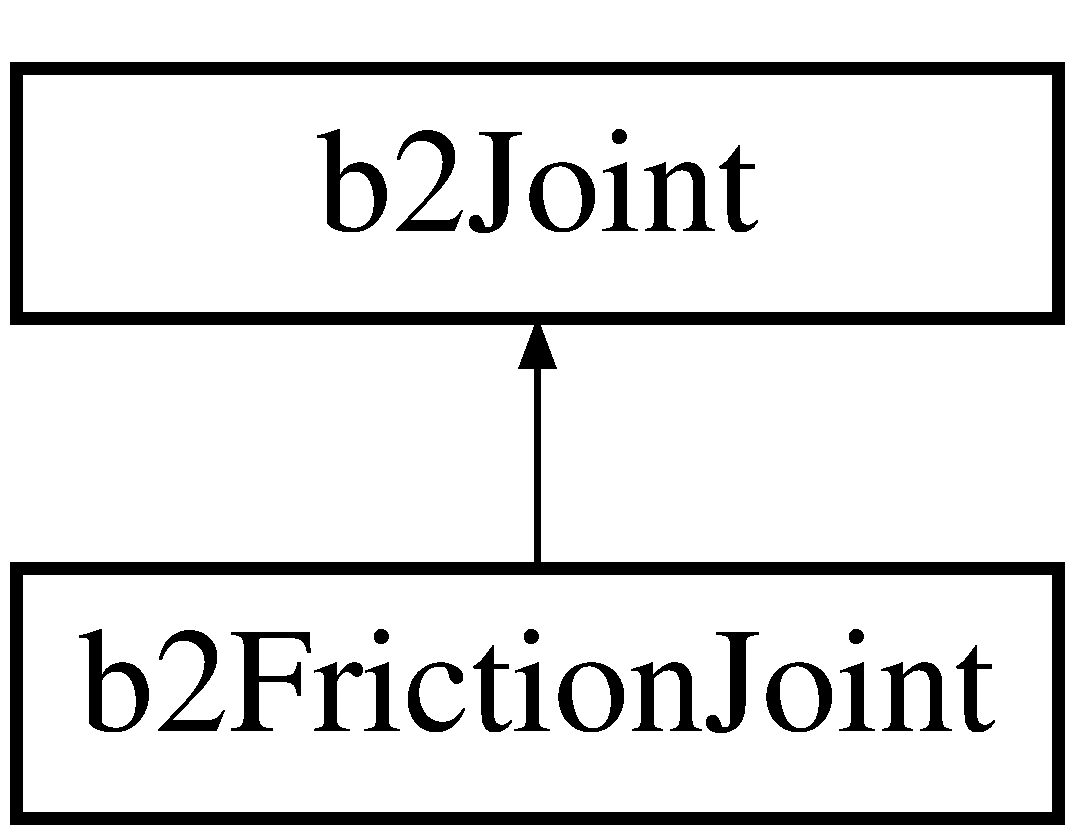
\includegraphics[height=2.000000cm]{classb2FrictionJoint}
\end{center}
\end{figure}
\subsection*{Public Member Functions}
\begin{DoxyCompactItemize}
\item 
\mbox{\Hypertarget{classb2FrictionJoint_a8e0bf2e9eba24f326d060789fedc7278}\label{classb2FrictionJoint_a8e0bf2e9eba24f326d060789fedc7278}} 
\mbox{\hyperlink{structb2Vec2}{b2\+Vec2}} \mbox{\hyperlink{classb2FrictionJoint_a8e0bf2e9eba24f326d060789fedc7278}{Get\+AnchorA}} () const override
\begin{DoxyCompactList}\small\item\em Get the anchor point on bodyA in world coordinates. \end{DoxyCompactList}\item 
\mbox{\Hypertarget{classb2FrictionJoint_af5a025b64221aafa98393d47d8414328}\label{classb2FrictionJoint_af5a025b64221aafa98393d47d8414328}} 
\mbox{\hyperlink{structb2Vec2}{b2\+Vec2}} \mbox{\hyperlink{classb2FrictionJoint_af5a025b64221aafa98393d47d8414328}{Get\+AnchorB}} () const override
\begin{DoxyCompactList}\small\item\em Get the anchor point on bodyB in world coordinates. \end{DoxyCompactList}\item 
\mbox{\Hypertarget{classb2FrictionJoint_a39d2c9ec06e6dd9733a8c4d72b4db2f0}\label{classb2FrictionJoint_a39d2c9ec06e6dd9733a8c4d72b4db2f0}} 
\mbox{\hyperlink{structb2Vec2}{b2\+Vec2}} \mbox{\hyperlink{classb2FrictionJoint_a39d2c9ec06e6dd9733a8c4d72b4db2f0}{Get\+Reaction\+Force}} (float32 inv\+\_\+dt) const override
\begin{DoxyCompactList}\small\item\em Get the reaction force on bodyB at the joint anchor in Newtons. \end{DoxyCompactList}\item 
\mbox{\Hypertarget{classb2FrictionJoint_a0a51dfa3bbc85408b9ccd63664230c99}\label{classb2FrictionJoint_a0a51dfa3bbc85408b9ccd63664230c99}} 
float32 \mbox{\hyperlink{classb2FrictionJoint_a0a51dfa3bbc85408b9ccd63664230c99}{Get\+Reaction\+Torque}} (float32 inv\+\_\+dt) const override
\begin{DoxyCompactList}\small\item\em Get the reaction torque on bodyB in N$\ast$m. \end{DoxyCompactList}\item 
\mbox{\Hypertarget{classb2FrictionJoint_a34023581ada2b4fba11e058695b49dd7}\label{classb2FrictionJoint_a34023581ada2b4fba11e058695b49dd7}} 
const \mbox{\hyperlink{structb2Vec2}{b2\+Vec2}} \& \mbox{\hyperlink{classb2FrictionJoint_a34023581ada2b4fba11e058695b49dd7}{Get\+Local\+AnchorA}} () const
\begin{DoxyCompactList}\small\item\em The local anchor point relative to bodyA\textquotesingle{}s origin. \end{DoxyCompactList}\item 
\mbox{\Hypertarget{classb2FrictionJoint_a44fab4532f7c4aad9d833f009caac586}\label{classb2FrictionJoint_a44fab4532f7c4aad9d833f009caac586}} 
const \mbox{\hyperlink{structb2Vec2}{b2\+Vec2}} \& \mbox{\hyperlink{classb2FrictionJoint_a44fab4532f7c4aad9d833f009caac586}{Get\+Local\+AnchorB}} () const
\begin{DoxyCompactList}\small\item\em The local anchor point relative to bodyB\textquotesingle{}s origin. \end{DoxyCompactList}\item 
\mbox{\Hypertarget{classb2FrictionJoint_a7936d852b5ad71dc92efc397865dda41}\label{classb2FrictionJoint_a7936d852b5ad71dc92efc397865dda41}} 
void \mbox{\hyperlink{classb2FrictionJoint_a7936d852b5ad71dc92efc397865dda41}{Set\+Max\+Force}} (float32 force)
\begin{DoxyCompactList}\small\item\em Set the maximum friction force in N. \end{DoxyCompactList}\item 
\mbox{\Hypertarget{classb2FrictionJoint_ad5f66e02841b8402e5560476c3c478c9}\label{classb2FrictionJoint_ad5f66e02841b8402e5560476c3c478c9}} 
float32 \mbox{\hyperlink{classb2FrictionJoint_ad5f66e02841b8402e5560476c3c478c9}{Get\+Max\+Force}} () const
\begin{DoxyCompactList}\small\item\em Get the maximum friction force in N. \end{DoxyCompactList}\item 
\mbox{\Hypertarget{classb2FrictionJoint_a9e3aaf485dc86a378bb62ee78cea43aa}\label{classb2FrictionJoint_a9e3aaf485dc86a378bb62ee78cea43aa}} 
void \mbox{\hyperlink{classb2FrictionJoint_a9e3aaf485dc86a378bb62ee78cea43aa}{Set\+Max\+Torque}} (float32 torque)
\begin{DoxyCompactList}\small\item\em Set the maximum friction torque in N$\ast$m. \end{DoxyCompactList}\item 
\mbox{\Hypertarget{classb2FrictionJoint_ae926972faa5846436cbcfe5772adc1f6}\label{classb2FrictionJoint_ae926972faa5846436cbcfe5772adc1f6}} 
float32 \mbox{\hyperlink{classb2FrictionJoint_ae926972faa5846436cbcfe5772adc1f6}{Get\+Max\+Torque}} () const
\begin{DoxyCompactList}\small\item\em Get the maximum friction torque in N$\ast$m. \end{DoxyCompactList}\item 
\mbox{\Hypertarget{classb2FrictionJoint_a934a3ce5bda09bc07111c1dd4e192406}\label{classb2FrictionJoint_a934a3ce5bda09bc07111c1dd4e192406}} 
void \mbox{\hyperlink{classb2FrictionJoint_a934a3ce5bda09bc07111c1dd4e192406}{Dump}} () override
\begin{DoxyCompactList}\small\item\em Dump joint to dm\+Log. \end{DoxyCompactList}\end{DoxyCompactItemize}
\subsection*{Protected Member Functions}
\begin{DoxyCompactItemize}
\item 
\mbox{\Hypertarget{classb2FrictionJoint_a7413c5f289257f0e993b7e750fe95b99}\label{classb2FrictionJoint_a7413c5f289257f0e993b7e750fe95b99}} 
{\bfseries b2\+Friction\+Joint} (const \mbox{\hyperlink{structb2FrictionJointDef}{b2\+Friction\+Joint\+Def}} $\ast$def)
\item 
\mbox{\Hypertarget{classb2FrictionJoint_afce4006666e83c50d2017b5ff5e7ca2d}\label{classb2FrictionJoint_afce4006666e83c50d2017b5ff5e7ca2d}} 
void {\bfseries Init\+Velocity\+Constraints} (const \mbox{\hyperlink{structb2SolverData}{b2\+Solver\+Data}} \&data) override
\item 
\mbox{\Hypertarget{classb2FrictionJoint_a49109c1785d949e99a809a8c297abf13}\label{classb2FrictionJoint_a49109c1785d949e99a809a8c297abf13}} 
void {\bfseries Solve\+Velocity\+Constraints} (const \mbox{\hyperlink{structb2SolverData}{b2\+Solver\+Data}} \&data) override
\item 
\mbox{\Hypertarget{classb2FrictionJoint_a4e4b64b634299136bc2c7096d5c28aa8}\label{classb2FrictionJoint_a4e4b64b634299136bc2c7096d5c28aa8}} 
bool {\bfseries Solve\+Position\+Constraints} (const \mbox{\hyperlink{structb2SolverData}{b2\+Solver\+Data}} \&data) override
\end{DoxyCompactItemize}
\subsection*{Protected Attributes}
\begin{DoxyCompactItemize}
\item 
\mbox{\Hypertarget{classb2FrictionJoint_a8842818b75319de1e4f3ec70d784dce1}\label{classb2FrictionJoint_a8842818b75319de1e4f3ec70d784dce1}} 
\mbox{\hyperlink{structb2Vec2}{b2\+Vec2}} {\bfseries m\+\_\+local\+AnchorA}
\item 
\mbox{\Hypertarget{classb2FrictionJoint_aa5920c253c6564bfd04a11e767f2e2db}\label{classb2FrictionJoint_aa5920c253c6564bfd04a11e767f2e2db}} 
\mbox{\hyperlink{structb2Vec2}{b2\+Vec2}} {\bfseries m\+\_\+local\+AnchorB}
\item 
\mbox{\Hypertarget{classb2FrictionJoint_ad4f8286af03b0f37a9eec7e9884d7e26}\label{classb2FrictionJoint_ad4f8286af03b0f37a9eec7e9884d7e26}} 
\mbox{\hyperlink{structb2Vec2}{b2\+Vec2}} {\bfseries m\+\_\+linear\+Impulse}
\item 
\mbox{\Hypertarget{classb2FrictionJoint_ab199dba9687ece4b816589b9e1e14750}\label{classb2FrictionJoint_ab199dba9687ece4b816589b9e1e14750}} 
float32 {\bfseries m\+\_\+angular\+Impulse}
\item 
\mbox{\Hypertarget{classb2FrictionJoint_ae666a8093844e2fb75e4c3de6b3f377a}\label{classb2FrictionJoint_ae666a8093844e2fb75e4c3de6b3f377a}} 
float32 {\bfseries m\+\_\+max\+Force}
\item 
\mbox{\Hypertarget{classb2FrictionJoint_a42b3ac5d34ab2399a5e4f0ea9afe988d}\label{classb2FrictionJoint_a42b3ac5d34ab2399a5e4f0ea9afe988d}} 
float32 {\bfseries m\+\_\+max\+Torque}
\item 
\mbox{\Hypertarget{classb2FrictionJoint_a069c815e1cdf78160cb96b4b0047f64e}\label{classb2FrictionJoint_a069c815e1cdf78160cb96b4b0047f64e}} 
int32 {\bfseries m\+\_\+indexA}
\item 
\mbox{\Hypertarget{classb2FrictionJoint_a378198c55100884de4587cb9ab22128f}\label{classb2FrictionJoint_a378198c55100884de4587cb9ab22128f}} 
int32 {\bfseries m\+\_\+indexB}
\item 
\mbox{\Hypertarget{classb2FrictionJoint_aa02b166017af5893b6b49b56dc96c70a}\label{classb2FrictionJoint_aa02b166017af5893b6b49b56dc96c70a}} 
\mbox{\hyperlink{structb2Vec2}{b2\+Vec2}} {\bfseries m\+\_\+rA}
\item 
\mbox{\Hypertarget{classb2FrictionJoint_a99b95a2dbfb119cbccccb137748aca44}\label{classb2FrictionJoint_a99b95a2dbfb119cbccccb137748aca44}} 
\mbox{\hyperlink{structb2Vec2}{b2\+Vec2}} {\bfseries m\+\_\+rB}
\item 
\mbox{\Hypertarget{classb2FrictionJoint_af732965abe1f29f7469e1ea17506218c}\label{classb2FrictionJoint_af732965abe1f29f7469e1ea17506218c}} 
\mbox{\hyperlink{structb2Vec2}{b2\+Vec2}} {\bfseries m\+\_\+local\+CenterA}
\item 
\mbox{\Hypertarget{classb2FrictionJoint_a55739866c1f3423caf2116e0a869ec45}\label{classb2FrictionJoint_a55739866c1f3423caf2116e0a869ec45}} 
\mbox{\hyperlink{structb2Vec2}{b2\+Vec2}} {\bfseries m\+\_\+local\+CenterB}
\item 
\mbox{\Hypertarget{classb2FrictionJoint_a7b7a482216efd081db94465db409fa21}\label{classb2FrictionJoint_a7b7a482216efd081db94465db409fa21}} 
float32 {\bfseries m\+\_\+inv\+MassA}
\item 
\mbox{\Hypertarget{classb2FrictionJoint_a189a3869e59f6b1e00c83fcaf6b08253}\label{classb2FrictionJoint_a189a3869e59f6b1e00c83fcaf6b08253}} 
float32 {\bfseries m\+\_\+inv\+MassB}
\item 
\mbox{\Hypertarget{classb2FrictionJoint_aad004207b7392e9828f55d8f15dc2aa8}\label{classb2FrictionJoint_aad004207b7392e9828f55d8f15dc2aa8}} 
float32 {\bfseries m\+\_\+inv\+IA}
\item 
\mbox{\Hypertarget{classb2FrictionJoint_a79ab8b49c2d4ce6415e3fe9376947d4c}\label{classb2FrictionJoint_a79ab8b49c2d4ce6415e3fe9376947d4c}} 
float32 {\bfseries m\+\_\+inv\+IB}
\item 
\mbox{\Hypertarget{classb2FrictionJoint_aa49bf4b20865a4976c3fae8398191182}\label{classb2FrictionJoint_aa49bf4b20865a4976c3fae8398191182}} 
\mbox{\hyperlink{structb2Mat22}{b2\+Mat22}} {\bfseries m\+\_\+linear\+Mass}
\item 
\mbox{\Hypertarget{classb2FrictionJoint_ab8f9aa5e516d90f1c80f92b0eb410c38}\label{classb2FrictionJoint_ab8f9aa5e516d90f1c80f92b0eb410c38}} 
float32 {\bfseries m\+\_\+angular\+Mass}
\end{DoxyCompactItemize}
\subsection*{Friends}
\begin{DoxyCompactItemize}
\item 
\mbox{\Hypertarget{classb2FrictionJoint_a54ade8ed3d794298108d7f4c4e4793fa}\label{classb2FrictionJoint_a54ade8ed3d794298108d7f4c4e4793fa}} 
class {\bfseries b2\+Joint}
\end{DoxyCompactItemize}
\subsection*{Additional Inherited Members}


\subsection{Detailed Description}
Friction joint. This is used for top-\/down friction. It provides 2D translational friction and angular friction. 

The documentation for this class was generated from the following files\+:\begin{DoxyCompactItemize}
\item 
Dynamics/\+Joints/b2\+Friction\+Joint.\+h\item 
Dynamics/\+Joints/b2\+Friction\+Joint.\+cpp\end{DoxyCompactItemize}

\hypertarget{structb2FrictionJointDef}{}\section{b2\+Friction\+Joint\+Def Struct Reference}
\label{structb2FrictionJointDef}\index{b2\+Friction\+Joint\+Def@{b2\+Friction\+Joint\+Def}}


Friction joint definition.  




{\ttfamily \#include $<$b2\+Friction\+Joint.\+h$>$}

Inheritance diagram for b2\+Friction\+Joint\+Def\+:\begin{figure}[H]
\begin{center}
\leavevmode
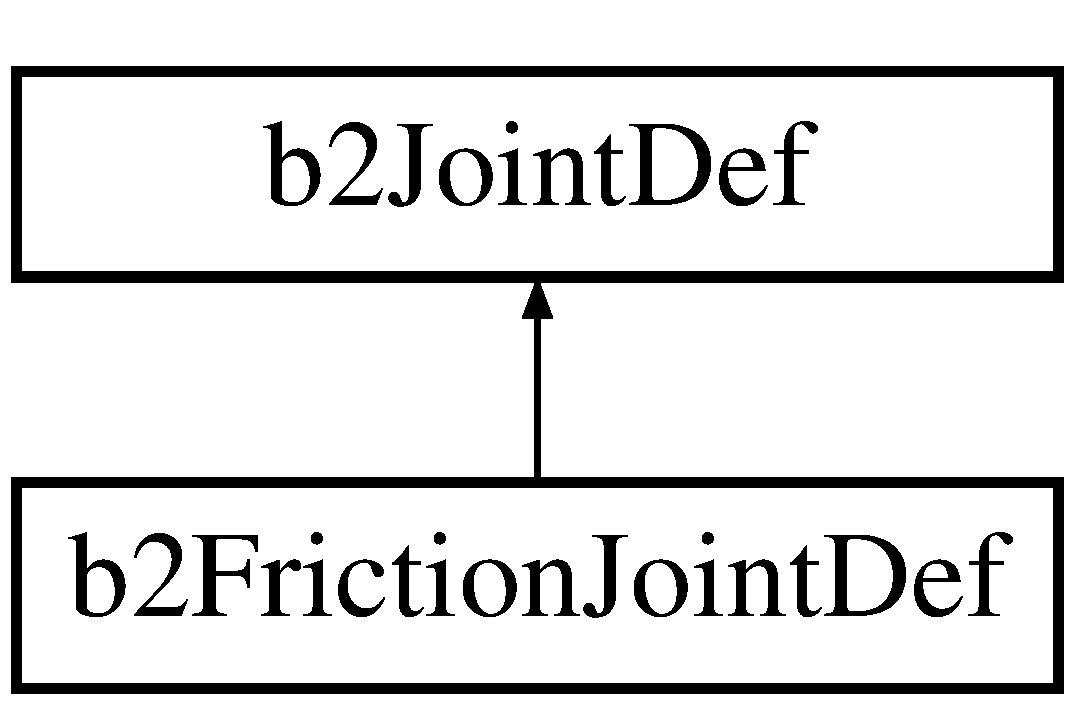
\includegraphics[height=2.000000cm]{structb2FrictionJointDef}
\end{center}
\end{figure}
\subsection*{Public Member Functions}
\begin{DoxyCompactItemize}
\item 
void \mbox{\hyperlink{structb2FrictionJointDef_aee104f2aeb34dec4e17e3c52a98f7915}{Initialize}} (\mbox{\hyperlink{classb2Body}{b2\+Body}} $\ast$\mbox{\hyperlink{structb2JointDef_a8cd54c93da396be75a9788f2c6897f05}{bodyA}}, \mbox{\hyperlink{classb2Body}{b2\+Body}} $\ast$\mbox{\hyperlink{structb2JointDef_aa4f4dee2fbcd12187b19506b60e68e3d}{bodyB}}, const \mbox{\hyperlink{structb2Vec2}{b2\+Vec2}} \&anchor)
\end{DoxyCompactItemize}
\subsection*{Public Attributes}
\begin{DoxyCompactItemize}
\item 
\mbox{\Hypertarget{structb2FrictionJointDef_a00b246e60ae282a956a42b662993e92a}\label{structb2FrictionJointDef_a00b246e60ae282a956a42b662993e92a}} 
\mbox{\hyperlink{structb2Vec2}{b2\+Vec2}} \mbox{\hyperlink{structb2FrictionJointDef_a00b246e60ae282a956a42b662993e92a}{local\+AnchorA}}
\begin{DoxyCompactList}\small\item\em The local anchor point relative to bodyA\textquotesingle{}s origin. \end{DoxyCompactList}\item 
\mbox{\Hypertarget{structb2FrictionJointDef_ad6d5a5614a7ac77b13e53fda3e32ed05}\label{structb2FrictionJointDef_ad6d5a5614a7ac77b13e53fda3e32ed05}} 
\mbox{\hyperlink{structb2Vec2}{b2\+Vec2}} \mbox{\hyperlink{structb2FrictionJointDef_ad6d5a5614a7ac77b13e53fda3e32ed05}{local\+AnchorB}}
\begin{DoxyCompactList}\small\item\em The local anchor point relative to bodyB\textquotesingle{}s origin. \end{DoxyCompactList}\item 
\mbox{\Hypertarget{structb2FrictionJointDef_ad30e97a80790d4ca64bac7a1fa7d1b35}\label{structb2FrictionJointDef_ad30e97a80790d4ca64bac7a1fa7d1b35}} 
float32 \mbox{\hyperlink{structb2FrictionJointDef_ad30e97a80790d4ca64bac7a1fa7d1b35}{max\+Force}}
\begin{DoxyCompactList}\small\item\em The maximum friction force in N. \end{DoxyCompactList}\item 
\mbox{\Hypertarget{structb2FrictionJointDef_a61adfb0ee7c0ed4cb8feee8304c16ef6}\label{structb2FrictionJointDef_a61adfb0ee7c0ed4cb8feee8304c16ef6}} 
float32 \mbox{\hyperlink{structb2FrictionJointDef_a61adfb0ee7c0ed4cb8feee8304c16ef6}{max\+Torque}}
\begin{DoxyCompactList}\small\item\em The maximum friction torque in N-\/m. \end{DoxyCompactList}\end{DoxyCompactItemize}


\subsection{Detailed Description}
Friction joint definition. 

\subsection{Member Function Documentation}
\mbox{\Hypertarget{structb2FrictionJointDef_aee104f2aeb34dec4e17e3c52a98f7915}\label{structb2FrictionJointDef_aee104f2aeb34dec4e17e3c52a98f7915}} 
\index{b2\+Friction\+Joint\+Def@{b2\+Friction\+Joint\+Def}!Initialize@{Initialize}}
\index{Initialize@{Initialize}!b2\+Friction\+Joint\+Def@{b2\+Friction\+Joint\+Def}}
\subsubsection{\texorpdfstring{Initialize()}{Initialize()}}
{\footnotesize\ttfamily void b2\+Friction\+Joint\+Def\+::\+Initialize (\begin{DoxyParamCaption}\item[{\mbox{\hyperlink{classb2Body}{b2\+Body}} $\ast$}]{bodyA,  }\item[{\mbox{\hyperlink{classb2Body}{b2\+Body}} $\ast$}]{bodyB,  }\item[{const \mbox{\hyperlink{structb2Vec2}{b2\+Vec2}} \&}]{anchor }\end{DoxyParamCaption})}

Initialize the bodies, anchors, axis, and reference angle using the world anchor and world axis. 

The documentation for this struct was generated from the following files\+:\begin{DoxyCompactItemize}
\item 
Dynamics/\+Joints/b2\+Friction\+Joint.\+h\item 
Dynamics/\+Joints/b2\+Friction\+Joint.\+cpp\end{DoxyCompactItemize}

\hypertarget{classb2GearJoint}{}\section{b2\+Gear\+Joint Class Reference}
\label{classb2GearJoint}\index{b2\+Gear\+Joint@{b2\+Gear\+Joint}}


{\ttfamily \#include $<$b2\+Gear\+Joint.\+h$>$}

Inheritance diagram for b2\+Gear\+Joint\+:\begin{figure}[H]
\begin{center}
\leavevmode
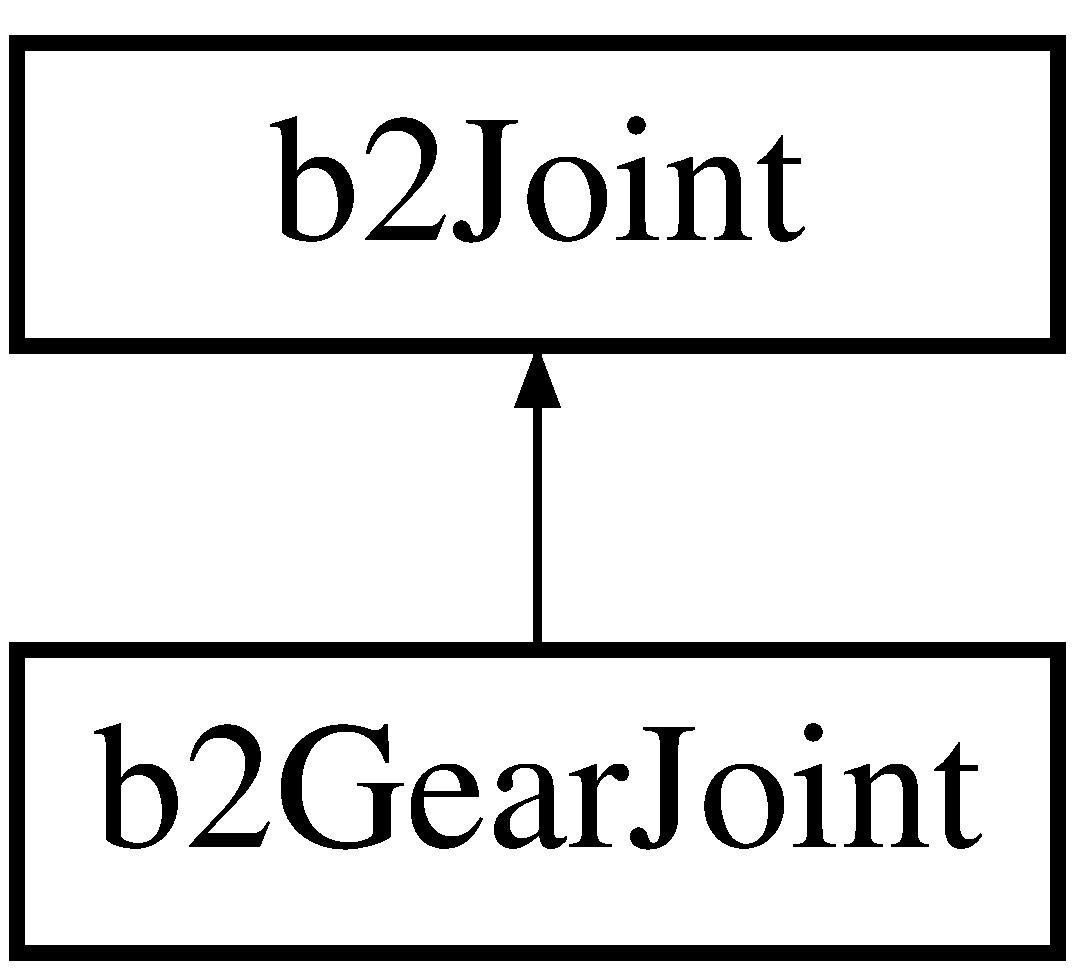
\includegraphics[height=2.000000cm]{classb2GearJoint}
\end{center}
\end{figure}
\subsection*{Public Member Functions}
\begin{DoxyCompactItemize}
\item 
\mbox{\Hypertarget{classb2GearJoint_a2928d2e9eac9137808537faa9b30a649}\label{classb2GearJoint_a2928d2e9eac9137808537faa9b30a649}} 
\mbox{\hyperlink{structb2Vec2}{b2\+Vec2}} \mbox{\hyperlink{classb2GearJoint_a2928d2e9eac9137808537faa9b30a649}{Get\+AnchorA}} () const override
\begin{DoxyCompactList}\small\item\em Get the anchor point on bodyA in world coordinates. \end{DoxyCompactList}\item 
\mbox{\Hypertarget{classb2GearJoint_a3d24a3265e64f36017404a36abcb7889}\label{classb2GearJoint_a3d24a3265e64f36017404a36abcb7889}} 
\mbox{\hyperlink{structb2Vec2}{b2\+Vec2}} \mbox{\hyperlink{classb2GearJoint_a3d24a3265e64f36017404a36abcb7889}{Get\+AnchorB}} () const override
\begin{DoxyCompactList}\small\item\em Get the anchor point on bodyB in world coordinates. \end{DoxyCompactList}\item 
\mbox{\Hypertarget{classb2GearJoint_aa1dc4c7c58d8ee656726c372edb7abcd}\label{classb2GearJoint_aa1dc4c7c58d8ee656726c372edb7abcd}} 
\mbox{\hyperlink{structb2Vec2}{b2\+Vec2}} \mbox{\hyperlink{classb2GearJoint_aa1dc4c7c58d8ee656726c372edb7abcd}{Get\+Reaction\+Force}} (float32 inv\+\_\+dt) const override
\begin{DoxyCompactList}\small\item\em Get the reaction force on bodyB at the joint anchor in Newtons. \end{DoxyCompactList}\item 
\mbox{\Hypertarget{classb2GearJoint_a6c0f2f34c087085202b1a9506cd48fd1}\label{classb2GearJoint_a6c0f2f34c087085202b1a9506cd48fd1}} 
float32 \mbox{\hyperlink{classb2GearJoint_a6c0f2f34c087085202b1a9506cd48fd1}{Get\+Reaction\+Torque}} (float32 inv\+\_\+dt) const override
\begin{DoxyCompactList}\small\item\em Get the reaction torque on bodyB in N$\ast$m. \end{DoxyCompactList}\item 
\mbox{\Hypertarget{classb2GearJoint_acd3fb38982319f387d1eb7aeddd5311f}\label{classb2GearJoint_acd3fb38982319f387d1eb7aeddd5311f}} 
\mbox{\hyperlink{classb2Joint}{b2\+Joint}} $\ast$ \mbox{\hyperlink{classb2GearJoint_acd3fb38982319f387d1eb7aeddd5311f}{Get\+Joint1}} ()
\begin{DoxyCompactList}\small\item\em Get the first joint. \end{DoxyCompactList}\item 
\mbox{\Hypertarget{classb2GearJoint_af1673b8edd80f3ae3b868c3a18b7b058}\label{classb2GearJoint_af1673b8edd80f3ae3b868c3a18b7b058}} 
\mbox{\hyperlink{classb2Joint}{b2\+Joint}} $\ast$ \mbox{\hyperlink{classb2GearJoint_af1673b8edd80f3ae3b868c3a18b7b058}{Get\+Joint2}} ()
\begin{DoxyCompactList}\small\item\em Get the second joint. \end{DoxyCompactList}\item 
\mbox{\Hypertarget{classb2GearJoint_a21c867bdc00c15ade2f399d370f92636}\label{classb2GearJoint_a21c867bdc00c15ade2f399d370f92636}} 
void \mbox{\hyperlink{classb2GearJoint_a21c867bdc00c15ade2f399d370f92636}{Set\+Ratio}} (float32 ratio)
\begin{DoxyCompactList}\small\item\em Set/\+Get the gear ratio. \end{DoxyCompactList}\item 
\mbox{\Hypertarget{classb2GearJoint_a46dffdce62bdf15a28c10a27d640bc10}\label{classb2GearJoint_a46dffdce62bdf15a28c10a27d640bc10}} 
float32 {\bfseries Get\+Ratio} () const
\item 
\mbox{\Hypertarget{classb2GearJoint_a40ca34a7853db14d3978c0b18598dd8d}\label{classb2GearJoint_a40ca34a7853db14d3978c0b18598dd8d}} 
void \mbox{\hyperlink{classb2GearJoint_a40ca34a7853db14d3978c0b18598dd8d}{Dump}} () override
\begin{DoxyCompactList}\small\item\em Dump joint to dm\+Log. \end{DoxyCompactList}\end{DoxyCompactItemize}
\subsection*{Protected Member Functions}
\begin{DoxyCompactItemize}
\item 
\mbox{\Hypertarget{classb2GearJoint_a4b247c79e74cb1e5b906527fe7d151ce}\label{classb2GearJoint_a4b247c79e74cb1e5b906527fe7d151ce}} 
{\bfseries b2\+Gear\+Joint} (const \mbox{\hyperlink{structb2GearJointDef}{b2\+Gear\+Joint\+Def}} $\ast$data)
\item 
\mbox{\Hypertarget{classb2GearJoint_ac3c76db6940bcb4c94d564960b9c57ab}\label{classb2GearJoint_ac3c76db6940bcb4c94d564960b9c57ab}} 
void {\bfseries Init\+Velocity\+Constraints} (const \mbox{\hyperlink{structb2SolverData}{b2\+Solver\+Data}} \&data) override
\item 
\mbox{\Hypertarget{classb2GearJoint_a25ff465354108f5ae2b60fb9f7836820}\label{classb2GearJoint_a25ff465354108f5ae2b60fb9f7836820}} 
void {\bfseries Solve\+Velocity\+Constraints} (const \mbox{\hyperlink{structb2SolverData}{b2\+Solver\+Data}} \&data) override
\item 
\mbox{\Hypertarget{classb2GearJoint_a85633bbab3c4b4cb862bccce7e0253c2}\label{classb2GearJoint_a85633bbab3c4b4cb862bccce7e0253c2}} 
bool {\bfseries Solve\+Position\+Constraints} (const \mbox{\hyperlink{structb2SolverData}{b2\+Solver\+Data}} \&data) override
\end{DoxyCompactItemize}
\subsection*{Protected Attributes}
\begin{DoxyCompactItemize}
\item 
\mbox{\Hypertarget{classb2GearJoint_a7694fc4574c774c22a8c202e0d49fd84}\label{classb2GearJoint_a7694fc4574c774c22a8c202e0d49fd84}} 
\mbox{\hyperlink{classb2Joint}{b2\+Joint}} $\ast$ {\bfseries m\+\_\+joint1}
\item 
\mbox{\Hypertarget{classb2GearJoint_a94290117dd4f2467eee49ecc150b9eb6}\label{classb2GearJoint_a94290117dd4f2467eee49ecc150b9eb6}} 
\mbox{\hyperlink{classb2Joint}{b2\+Joint}} $\ast$ {\bfseries m\+\_\+joint2}
\item 
\mbox{\Hypertarget{classb2GearJoint_a0819b72c766d69cb1995f6cca4e98853}\label{classb2GearJoint_a0819b72c766d69cb1995f6cca4e98853}} 
b2\+Joint\+Type {\bfseries m\+\_\+typeA}
\item 
\mbox{\Hypertarget{classb2GearJoint_a03e1959e04a361db79ae5da5ba76379e}\label{classb2GearJoint_a03e1959e04a361db79ae5da5ba76379e}} 
b2\+Joint\+Type {\bfseries m\+\_\+typeB}
\item 
\mbox{\Hypertarget{classb2GearJoint_a07e5f85b71bf335552835989dc013fe6}\label{classb2GearJoint_a07e5f85b71bf335552835989dc013fe6}} 
\mbox{\hyperlink{classb2Body}{b2\+Body}} $\ast$ {\bfseries m\+\_\+bodyC}
\item 
\mbox{\Hypertarget{classb2GearJoint_ad3a1795c11b652b4b2f8bfc3ed96cb0b}\label{classb2GearJoint_ad3a1795c11b652b4b2f8bfc3ed96cb0b}} 
\mbox{\hyperlink{classb2Body}{b2\+Body}} $\ast$ {\bfseries m\+\_\+bodyD}
\item 
\mbox{\Hypertarget{classb2GearJoint_acac78f2e3730fda540d1c7a74889bfc5}\label{classb2GearJoint_acac78f2e3730fda540d1c7a74889bfc5}} 
\mbox{\hyperlink{structb2Vec2}{b2\+Vec2}} {\bfseries m\+\_\+local\+AnchorA}
\item 
\mbox{\Hypertarget{classb2GearJoint_a864c3d4d7944f72783a073993530d9fd}\label{classb2GearJoint_a864c3d4d7944f72783a073993530d9fd}} 
\mbox{\hyperlink{structb2Vec2}{b2\+Vec2}} {\bfseries m\+\_\+local\+AnchorB}
\item 
\mbox{\Hypertarget{classb2GearJoint_a9361797683a30e70afd5b8690fe47ba3}\label{classb2GearJoint_a9361797683a30e70afd5b8690fe47ba3}} 
\mbox{\hyperlink{structb2Vec2}{b2\+Vec2}} {\bfseries m\+\_\+local\+AnchorC}
\item 
\mbox{\Hypertarget{classb2GearJoint_abdd5be52535b5b56e44fc27832d057d2}\label{classb2GearJoint_abdd5be52535b5b56e44fc27832d057d2}} 
\mbox{\hyperlink{structb2Vec2}{b2\+Vec2}} {\bfseries m\+\_\+local\+AnchorD}
\item 
\mbox{\Hypertarget{classb2GearJoint_a52ae3b3a06ad9dae6b3201404784cc18}\label{classb2GearJoint_a52ae3b3a06ad9dae6b3201404784cc18}} 
\mbox{\hyperlink{structb2Vec2}{b2\+Vec2}} {\bfseries m\+\_\+local\+AxisC}
\item 
\mbox{\Hypertarget{classb2GearJoint_a49cc9f1b74793dce3311cf7a35a8aee1}\label{classb2GearJoint_a49cc9f1b74793dce3311cf7a35a8aee1}} 
\mbox{\hyperlink{structb2Vec2}{b2\+Vec2}} {\bfseries m\+\_\+local\+AxisD}
\item 
\mbox{\Hypertarget{classb2GearJoint_a1ba0c6172cd2dd2017813bab7d1b268b}\label{classb2GearJoint_a1ba0c6172cd2dd2017813bab7d1b268b}} 
float32 {\bfseries m\+\_\+reference\+AngleA}
\item 
\mbox{\Hypertarget{classb2GearJoint_a553920f723a1b7a38fd1d671101c5e4e}\label{classb2GearJoint_a553920f723a1b7a38fd1d671101c5e4e}} 
float32 {\bfseries m\+\_\+reference\+AngleB}
\item 
\mbox{\Hypertarget{classb2GearJoint_af67d237380cdcbfe93053b1ceb72f17b}\label{classb2GearJoint_af67d237380cdcbfe93053b1ceb72f17b}} 
float32 {\bfseries m\+\_\+constant}
\item 
\mbox{\Hypertarget{classb2GearJoint_ad6b9106922b65f873dd02c6e68e6778a}\label{classb2GearJoint_ad6b9106922b65f873dd02c6e68e6778a}} 
float32 {\bfseries m\+\_\+ratio}
\item 
\mbox{\Hypertarget{classb2GearJoint_ae19e7fb67c7623f39776f1160b76d62f}\label{classb2GearJoint_ae19e7fb67c7623f39776f1160b76d62f}} 
float32 {\bfseries m\+\_\+impulse}
\item 
\mbox{\Hypertarget{classb2GearJoint_adb00e71e60a222e432b57c95c38b8bd7}\label{classb2GearJoint_adb00e71e60a222e432b57c95c38b8bd7}} 
int32 {\bfseries m\+\_\+indexA}
\item 
\mbox{\Hypertarget{classb2GearJoint_a5cf185f4e4b5d5e1780ba2c085ec2e6e}\label{classb2GearJoint_a5cf185f4e4b5d5e1780ba2c085ec2e6e}} 
int32 {\bfseries m\+\_\+indexB}
\item 
\mbox{\Hypertarget{classb2GearJoint_a46528e9a9a33a4d67dd5b2abb3d1dec5}\label{classb2GearJoint_a46528e9a9a33a4d67dd5b2abb3d1dec5}} 
int32 {\bfseries m\+\_\+indexC}
\item 
\mbox{\Hypertarget{classb2GearJoint_a068be34dbdf39ac59c7a5bb7777d550f}\label{classb2GearJoint_a068be34dbdf39ac59c7a5bb7777d550f}} 
int32 {\bfseries m\+\_\+indexD}
\item 
\mbox{\Hypertarget{classb2GearJoint_afb46a5545846cc085f2aad02a05acc86}\label{classb2GearJoint_afb46a5545846cc085f2aad02a05acc86}} 
\mbox{\hyperlink{structb2Vec2}{b2\+Vec2}} {\bfseries m\+\_\+lcA}
\item 
\mbox{\Hypertarget{classb2GearJoint_a4f933756b7e6b9ec060b105d0fb6689b}\label{classb2GearJoint_a4f933756b7e6b9ec060b105d0fb6689b}} 
\mbox{\hyperlink{structb2Vec2}{b2\+Vec2}} {\bfseries m\+\_\+lcB}
\item 
\mbox{\Hypertarget{classb2GearJoint_a9eaca477247eb71dae06f12842bc636d}\label{classb2GearJoint_a9eaca477247eb71dae06f12842bc636d}} 
\mbox{\hyperlink{structb2Vec2}{b2\+Vec2}} {\bfseries m\+\_\+lcC}
\item 
\mbox{\Hypertarget{classb2GearJoint_a21c4c7aa8c0ba7ccf9d4f786a31e5553}\label{classb2GearJoint_a21c4c7aa8c0ba7ccf9d4f786a31e5553}} 
\mbox{\hyperlink{structb2Vec2}{b2\+Vec2}} {\bfseries m\+\_\+lcD}
\item 
\mbox{\Hypertarget{classb2GearJoint_a5f425a3ff6a4d08090be512ee56993c5}\label{classb2GearJoint_a5f425a3ff6a4d08090be512ee56993c5}} 
float32 {\bfseries m\+\_\+mA}
\item 
\mbox{\Hypertarget{classb2GearJoint_a83985722b901f36b59e29b98c2bbb1af}\label{classb2GearJoint_a83985722b901f36b59e29b98c2bbb1af}} 
float32 {\bfseries m\+\_\+mB}
\item 
\mbox{\Hypertarget{classb2GearJoint_a79253d1b43531e5acdf36a3f710c583a}\label{classb2GearJoint_a79253d1b43531e5acdf36a3f710c583a}} 
float32 {\bfseries m\+\_\+mC}
\item 
\mbox{\Hypertarget{classb2GearJoint_a7a3685b9bb07b2d81c58b96ff662c5ce}\label{classb2GearJoint_a7a3685b9bb07b2d81c58b96ff662c5ce}} 
float32 {\bfseries m\+\_\+mD}
\item 
\mbox{\Hypertarget{classb2GearJoint_a138784eb59950e25125e45087945b717}\label{classb2GearJoint_a138784eb59950e25125e45087945b717}} 
float32 {\bfseries m\+\_\+iA}
\item 
\mbox{\Hypertarget{classb2GearJoint_acca792262071441bd6fbfc891fcaf942}\label{classb2GearJoint_acca792262071441bd6fbfc891fcaf942}} 
float32 {\bfseries m\+\_\+iB}
\item 
\mbox{\Hypertarget{classb2GearJoint_ac4e6493093914f78e0c8f79248041a1c}\label{classb2GearJoint_ac4e6493093914f78e0c8f79248041a1c}} 
float32 {\bfseries m\+\_\+iC}
\item 
\mbox{\Hypertarget{classb2GearJoint_ad05416c4e98a30e4eb9297ff20b38c1a}\label{classb2GearJoint_ad05416c4e98a30e4eb9297ff20b38c1a}} 
float32 {\bfseries m\+\_\+iD}
\item 
\mbox{\Hypertarget{classb2GearJoint_a23eb9f668936f931d40f930e085dd5a0}\label{classb2GearJoint_a23eb9f668936f931d40f930e085dd5a0}} 
\mbox{\hyperlink{structb2Vec2}{b2\+Vec2}} {\bfseries m\+\_\+\+Jv\+AC}
\item 
\mbox{\Hypertarget{classb2GearJoint_ab00b00c061d8b9e461f76ac4d72aac8c}\label{classb2GearJoint_ab00b00c061d8b9e461f76ac4d72aac8c}} 
\mbox{\hyperlink{structb2Vec2}{b2\+Vec2}} {\bfseries m\+\_\+\+Jv\+BD}
\item 
\mbox{\Hypertarget{classb2GearJoint_a3774fc69538e658f123d9437934aed70}\label{classb2GearJoint_a3774fc69538e658f123d9437934aed70}} 
float32 {\bfseries m\+\_\+\+JwA}
\item 
\mbox{\Hypertarget{classb2GearJoint_afcdb0ebe31ff8039771d006f4b87645c}\label{classb2GearJoint_afcdb0ebe31ff8039771d006f4b87645c}} 
float32 {\bfseries m\+\_\+\+JwB}
\item 
\mbox{\Hypertarget{classb2GearJoint_ac9b8f418c8f79392049afdf18aa6dc3e}\label{classb2GearJoint_ac9b8f418c8f79392049afdf18aa6dc3e}} 
float32 {\bfseries m\+\_\+\+JwC}
\item 
\mbox{\Hypertarget{classb2GearJoint_ac2d00521ef5f7c27b1747ad54d4ad5c2}\label{classb2GearJoint_ac2d00521ef5f7c27b1747ad54d4ad5c2}} 
float32 {\bfseries m\+\_\+\+JwD}
\item 
\mbox{\Hypertarget{classb2GearJoint_a71ac3578918bc97d257d652777b6b87f}\label{classb2GearJoint_a71ac3578918bc97d257d652777b6b87f}} 
float32 {\bfseries m\+\_\+mass}
\end{DoxyCompactItemize}
\subsection*{Friends}
\begin{DoxyCompactItemize}
\item 
\mbox{\Hypertarget{classb2GearJoint_a54ade8ed3d794298108d7f4c4e4793fa}\label{classb2GearJoint_a54ade8ed3d794298108d7f4c4e4793fa}} 
class {\bfseries b2\+Joint}
\end{DoxyCompactItemize}
\subsection*{Additional Inherited Members}


\subsection{Detailed Description}
A gear joint is used to connect two joints together. Either joint can be a revolute or prismatic joint. You specify a gear ratio to bind the motions together\+: coordinate1 + ratio $\ast$ coordinate2 = constant The ratio can be negative or positive. If one joint is a revolute joint and the other joint is a prismatic joint, then the ratio will have units of length or units of 1/length. \begin{DoxyWarning}{Warning}
You have to manually destroy the gear joint if joint1 or joint2 is destroyed. 
\end{DoxyWarning}


The documentation for this class was generated from the following files\+:\begin{DoxyCompactItemize}
\item 
Dynamics/\+Joints/b2\+Gear\+Joint.\+h\item 
Dynamics/\+Joints/b2\+Gear\+Joint.\+cpp\end{DoxyCompactItemize}

\hypertarget{structb2GearJointDef}{}\section{b2\+Gear\+Joint\+Def Struct Reference}
\label{structb2GearJointDef}\index{b2\+Gear\+Joint\+Def@{b2\+Gear\+Joint\+Def}}


{\ttfamily \#include $<$b2\+Gear\+Joint.\+h$>$}

Inheritance diagram for b2\+Gear\+Joint\+Def\+:\begin{figure}[H]
\begin{center}
\leavevmode
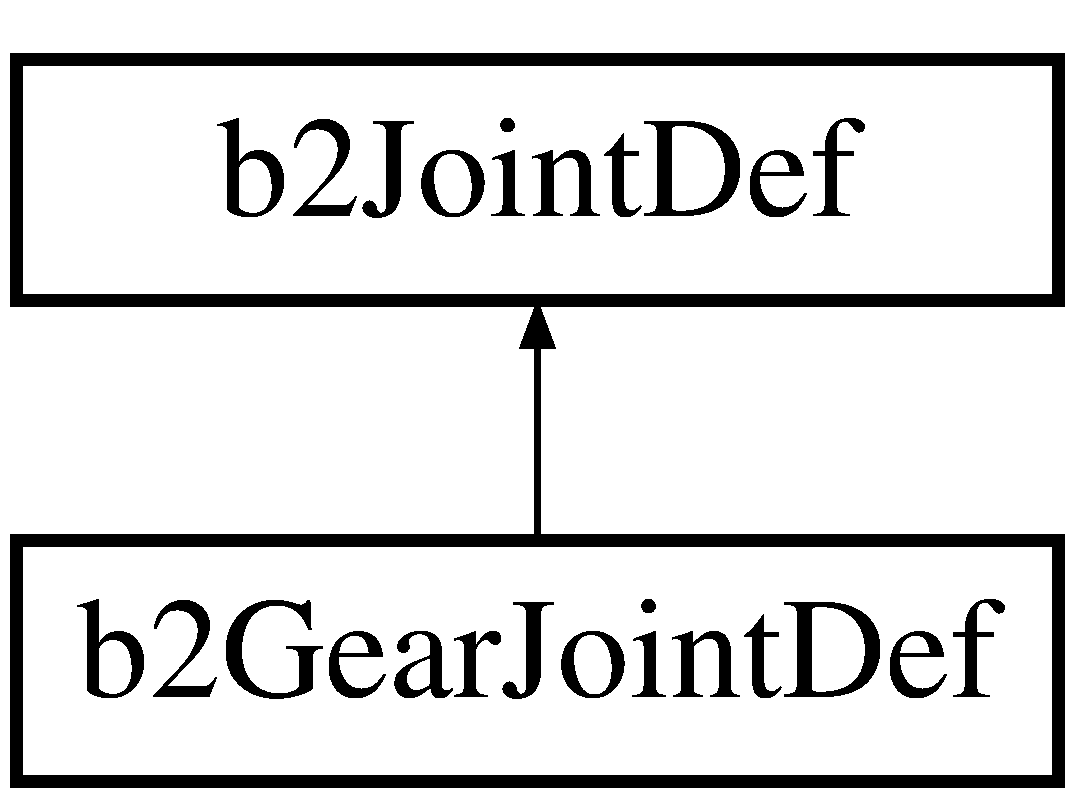
\includegraphics[height=2.000000cm]{structb2GearJointDef}
\end{center}
\end{figure}
\subsection*{Public Attributes}
\begin{DoxyCompactItemize}
\item 
\mbox{\Hypertarget{structb2GearJointDef_ae42d33b54291a9e256f3810926883473}\label{structb2GearJointDef_ae42d33b54291a9e256f3810926883473}} 
\mbox{\hyperlink{classb2Joint}{b2\+Joint}} $\ast$ \mbox{\hyperlink{structb2GearJointDef_ae42d33b54291a9e256f3810926883473}{joint1}}
\begin{DoxyCompactList}\small\item\em The first revolute/prismatic joint attached to the gear joint. \end{DoxyCompactList}\item 
\mbox{\Hypertarget{structb2GearJointDef_a73cf056fe40e63355073a01b097f4c82}\label{structb2GearJointDef_a73cf056fe40e63355073a01b097f4c82}} 
\mbox{\hyperlink{classb2Joint}{b2\+Joint}} $\ast$ \mbox{\hyperlink{structb2GearJointDef_a73cf056fe40e63355073a01b097f4c82}{joint2}}
\begin{DoxyCompactList}\small\item\em The second revolute/prismatic joint attached to the gear joint. \end{DoxyCompactList}\item 
float32 \mbox{\hyperlink{structb2GearJointDef_a57e9f4b6ce1ddc8b89b8455515f69323}{ratio}}
\end{DoxyCompactItemize}


\subsection{Detailed Description}
Gear joint definition. This definition requires two existing revolute or prismatic joints (any combination will work). 

\subsection{Member Data Documentation}
\mbox{\Hypertarget{structb2GearJointDef_a57e9f4b6ce1ddc8b89b8455515f69323}\label{structb2GearJointDef_a57e9f4b6ce1ddc8b89b8455515f69323}} 
\index{b2\+Gear\+Joint\+Def@{b2\+Gear\+Joint\+Def}!ratio@{ratio}}
\index{ratio@{ratio}!b2\+Gear\+Joint\+Def@{b2\+Gear\+Joint\+Def}}
\subsubsection{\texorpdfstring{ratio}{ratio}}
{\footnotesize\ttfamily float32 b2\+Gear\+Joint\+Def\+::ratio}

The gear ratio. \begin{DoxySeeAlso}{See also}
\mbox{\hyperlink{classb2GearJoint}{b2\+Gear\+Joint}} for explanation. 
\end{DoxySeeAlso}


The documentation for this struct was generated from the following file\+:\begin{DoxyCompactItemize}
\item 
Dynamics/\+Joints/b2\+Gear\+Joint.\+h\end{DoxyCompactItemize}

\hypertarget{classb2GrowableStack}{}\section{b2\+Growable\+Stack$<$ T, N $>$ Class Template Reference}
\label{classb2GrowableStack}\index{b2\+Growable\+Stack$<$ T, N $>$@{b2\+Growable\+Stack$<$ T, N $>$}}


{\ttfamily \#include $<$b2\+Growable\+Stack.\+h$>$}

\subsection*{Public Member Functions}
\begin{DoxyCompactItemize}
\item 
\mbox{\Hypertarget{classb2GrowableStack_a23661327d64ff72d1ec8d6bcdb6d8992}\label{classb2GrowableStack_a23661327d64ff72d1ec8d6bcdb6d8992}} 
void {\bfseries Push} (const T \&element)
\item 
\mbox{\Hypertarget{classb2GrowableStack_a53e53dcd6bff8308405a881f02957bc8}\label{classb2GrowableStack_a53e53dcd6bff8308405a881f02957bc8}} 
T {\bfseries Pop} ()
\item 
\mbox{\Hypertarget{classb2GrowableStack_a3049e76ba7182b988450bfe94d30d5aa}\label{classb2GrowableStack_a3049e76ba7182b988450bfe94d30d5aa}} 
int32 {\bfseries Get\+Count} ()
\end{DoxyCompactItemize}
\subsection*{Private Attributes}
\begin{DoxyCompactItemize}
\item 
\mbox{\Hypertarget{classb2GrowableStack_a0ffe2286a06066938a7413cef5689e7d}\label{classb2GrowableStack_a0ffe2286a06066938a7413cef5689e7d}} 
T $\ast$ {\bfseries m\+\_\+stack}
\item 
\mbox{\Hypertarget{classb2GrowableStack_a0df427a912ca2e6d8eecfc10e84162b3}\label{classb2GrowableStack_a0df427a912ca2e6d8eecfc10e84162b3}} 
T {\bfseries m\+\_\+array} \mbox{[}N\mbox{]}
\item 
\mbox{\Hypertarget{classb2GrowableStack_ab1ac57e30436c7501677143e0d7a051b}\label{classb2GrowableStack_ab1ac57e30436c7501677143e0d7a051b}} 
int32 {\bfseries m\+\_\+count}
\item 
\mbox{\Hypertarget{classb2GrowableStack_aede2309b9194c72f7096da16e2bb8c0a}\label{classb2GrowableStack_aede2309b9194c72f7096da16e2bb8c0a}} 
int32 {\bfseries m\+\_\+capacity}
\end{DoxyCompactItemize}


\subsection{Detailed Description}
\subsubsection*{template$<$typename T, int32 N$>$\newline
class b2\+Growable\+Stack$<$ T, N $>$}

This is a growable L\+I\+FO stack with an initial capacity of N. If the stack size exceeds the initial capacity, the heap is used to increase the size of the stack. 

The documentation for this class was generated from the following file\+:\begin{DoxyCompactItemize}
\item 
Common/b2\+Growable\+Stack.\+h\end{DoxyCompactItemize}

\hypertarget{classb2Island}{}\section{b2\+Island Class Reference}
\label{classb2Island}\index{b2\+Island@{b2\+Island}}


This is an internal class.  




{\ttfamily \#include $<$b2\+Island.\+h$>$}

\subsection*{Public Member Functions}
\begin{DoxyCompactItemize}
\item 
\mbox{\Hypertarget{classb2Island_a2f2258f09d2663dcb35a1d69d16896cb}\label{classb2Island_a2f2258f09d2663dcb35a1d69d16896cb}} 
{\bfseries b2\+Island} (int32 body\+Capacity, int32 contact\+Capacity, int32 joint\+Capacity, \mbox{\hyperlink{classb2StackAllocator}{b2\+Stack\+Allocator}} $\ast$allocator, \mbox{\hyperlink{classb2ContactListener}{b2\+Contact\+Listener}} $\ast$listener)
\item 
\mbox{\Hypertarget{classb2Island_a26566f7388fcaf7523446e5e76d99c4d}\label{classb2Island_a26566f7388fcaf7523446e5e76d99c4d}} 
void {\bfseries Clear} ()
\item 
\mbox{\Hypertarget{classb2Island_a28a6f74174cde3a6e93663c740f418fa}\label{classb2Island_a28a6f74174cde3a6e93663c740f418fa}} 
void {\bfseries Solve} (\mbox{\hyperlink{structb2Profile}{b2\+Profile}} $\ast$profile, const \mbox{\hyperlink{structb2TimeStep}{b2\+Time\+Step}} \&step, const \mbox{\hyperlink{structb2Vec2}{b2\+Vec2}} \&gravity, bool allow\+Sleep)
\item 
\mbox{\Hypertarget{classb2Island_a61f577b473962bb0d8add1f55eeef7ee}\label{classb2Island_a61f577b473962bb0d8add1f55eeef7ee}} 
void {\bfseries Solve\+T\+OI} (const \mbox{\hyperlink{structb2TimeStep}{b2\+Time\+Step}} \&sub\+Step, int32 toi\+IndexA, int32 toi\+IndexB)
\item 
\mbox{\Hypertarget{classb2Island_af2d54861bd063051c0a6dc5f73b27c3e}\label{classb2Island_af2d54861bd063051c0a6dc5f73b27c3e}} 
void {\bfseries Add} (\mbox{\hyperlink{classb2Body}{b2\+Body}} $\ast$body)
\item 
\mbox{\Hypertarget{classb2Island_abc0ea9208e818b551404fd507f197a51}\label{classb2Island_abc0ea9208e818b551404fd507f197a51}} 
void {\bfseries Add} (\mbox{\hyperlink{classb2Contact}{b2\+Contact}} $\ast$contact)
\item 
\mbox{\Hypertarget{classb2Island_a04e6ccd0c11f6ef5a7ed0a926d081445}\label{classb2Island_a04e6ccd0c11f6ef5a7ed0a926d081445}} 
void {\bfseries Add} (\mbox{\hyperlink{classb2Joint}{b2\+Joint}} $\ast$joint)
\item 
\mbox{\Hypertarget{classb2Island_a57620f76faf000f61c76e925e40e6129}\label{classb2Island_a57620f76faf000f61c76e925e40e6129}} 
void {\bfseries Report} (const \mbox{\hyperlink{structb2ContactVelocityConstraint}{b2\+Contact\+Velocity\+Constraint}} $\ast$constraints)
\end{DoxyCompactItemize}
\subsection*{Public Attributes}
\begin{DoxyCompactItemize}
\item 
\mbox{\Hypertarget{classb2Island_a5e28f216c0a12548c04491ab1d73c958}\label{classb2Island_a5e28f216c0a12548c04491ab1d73c958}} 
\mbox{\hyperlink{classb2StackAllocator}{b2\+Stack\+Allocator}} $\ast$ {\bfseries m\+\_\+allocator}
\item 
\mbox{\Hypertarget{classb2Island_aeba73fe42839d0361524d98e330e8e66}\label{classb2Island_aeba73fe42839d0361524d98e330e8e66}} 
\mbox{\hyperlink{classb2ContactListener}{b2\+Contact\+Listener}} $\ast$ {\bfseries m\+\_\+listener}
\item 
\mbox{\Hypertarget{classb2Island_ac9c65abf14c88e8a52fdd2c5cb56c5f4}\label{classb2Island_ac9c65abf14c88e8a52fdd2c5cb56c5f4}} 
\mbox{\hyperlink{classb2Body}{b2\+Body}} $\ast$$\ast$ {\bfseries m\+\_\+bodies}
\item 
\mbox{\Hypertarget{classb2Island_a49499a350859768a0c3f7b29fb091422}\label{classb2Island_a49499a350859768a0c3f7b29fb091422}} 
\mbox{\hyperlink{classb2Contact}{b2\+Contact}} $\ast$$\ast$ {\bfseries m\+\_\+contacts}
\item 
\mbox{\Hypertarget{classb2Island_a6653da11b66de22d8ba5db531c11b373}\label{classb2Island_a6653da11b66de22d8ba5db531c11b373}} 
\mbox{\hyperlink{classb2Joint}{b2\+Joint}} $\ast$$\ast$ {\bfseries m\+\_\+joints}
\item 
\mbox{\Hypertarget{classb2Island_a0f05bd177cf942ddfb494b17ec09b874}\label{classb2Island_a0f05bd177cf942ddfb494b17ec09b874}} 
\mbox{\hyperlink{structb2Position}{b2\+Position}} $\ast$ {\bfseries m\+\_\+positions}
\item 
\mbox{\Hypertarget{classb2Island_ae6a42be7ce4c03724a6da17d96cacb9f}\label{classb2Island_ae6a42be7ce4c03724a6da17d96cacb9f}} 
\mbox{\hyperlink{structb2Velocity}{b2\+Velocity}} $\ast$ {\bfseries m\+\_\+velocities}
\item 
\mbox{\Hypertarget{classb2Island_af78d066321e18cd8a4e409c4539ccb81}\label{classb2Island_af78d066321e18cd8a4e409c4539ccb81}} 
int32 {\bfseries m\+\_\+body\+Count}
\item 
\mbox{\Hypertarget{classb2Island_a913c91afb35ff717c7dd5b0aa1559e5b}\label{classb2Island_a913c91afb35ff717c7dd5b0aa1559e5b}} 
int32 {\bfseries m\+\_\+joint\+Count}
\item 
\mbox{\Hypertarget{classb2Island_ab5bad98e18356b15a68733be07b98abf}\label{classb2Island_ab5bad98e18356b15a68733be07b98abf}} 
int32 {\bfseries m\+\_\+contact\+Count}
\item 
\mbox{\Hypertarget{classb2Island_a5ea371889bb93fb6387ff2ab427191ed}\label{classb2Island_a5ea371889bb93fb6387ff2ab427191ed}} 
int32 {\bfseries m\+\_\+body\+Capacity}
\item 
\mbox{\Hypertarget{classb2Island_a1a65b8fc8256ca443f85e6ae6f2d841a}\label{classb2Island_a1a65b8fc8256ca443f85e6ae6f2d841a}} 
int32 {\bfseries m\+\_\+contact\+Capacity}
\item 
\mbox{\Hypertarget{classb2Island_a9b6e63c89307d469e1075585d65a9bbb}\label{classb2Island_a9b6e63c89307d469e1075585d65a9bbb}} 
int32 {\bfseries m\+\_\+joint\+Capacity}
\end{DoxyCompactItemize}


\subsection{Detailed Description}
This is an internal class. 

The documentation for this class was generated from the following files\+:\begin{DoxyCompactItemize}
\item 
Dynamics/b2\+Island.\+h\item 
Dynamics/b2\+Island.\+cpp\end{DoxyCompactItemize}

\hypertarget{structb2Jacobian}{}\section{b2\+Jacobian Struct Reference}
\label{structb2Jacobian}\index{b2\+Jacobian@{b2\+Jacobian}}
\subsection*{Public Attributes}
\begin{DoxyCompactItemize}
\item 
\mbox{\Hypertarget{structb2Jacobian_aa63199b443d411972b9cb6aac6c7cb34}\label{structb2Jacobian_aa63199b443d411972b9cb6aac6c7cb34}} 
\mbox{\hyperlink{structb2Vec2}{b2\+Vec2}} {\bfseries linear}
\item 
\mbox{\Hypertarget{structb2Jacobian_a0669f849afcdc154b36f86cb0529d2bc}\label{structb2Jacobian_a0669f849afcdc154b36f86cb0529d2bc}} 
float32 {\bfseries angularA}
\item 
\mbox{\Hypertarget{structb2Jacobian_a3bbdbd8e46f4fa9be2e50434edaaeb14}\label{structb2Jacobian_a3bbdbd8e46f4fa9be2e50434edaaeb14}} 
float32 {\bfseries angularB}
\end{DoxyCompactItemize}


The documentation for this struct was generated from the following file\+:\begin{DoxyCompactItemize}
\item 
Dynamics/\+Joints/b2\+Joint.\+h\end{DoxyCompactItemize}

\hypertarget{classb2Joint}{}\section{b2\+Joint Class Reference}
\label{classb2Joint}\index{b2\+Joint@{b2\+Joint}}


{\ttfamily \#include $<$b2\+Joint.\+h$>$}

Inheritance diagram for b2\+Joint\+:\begin{figure}[H]
\begin{center}
\leavevmode
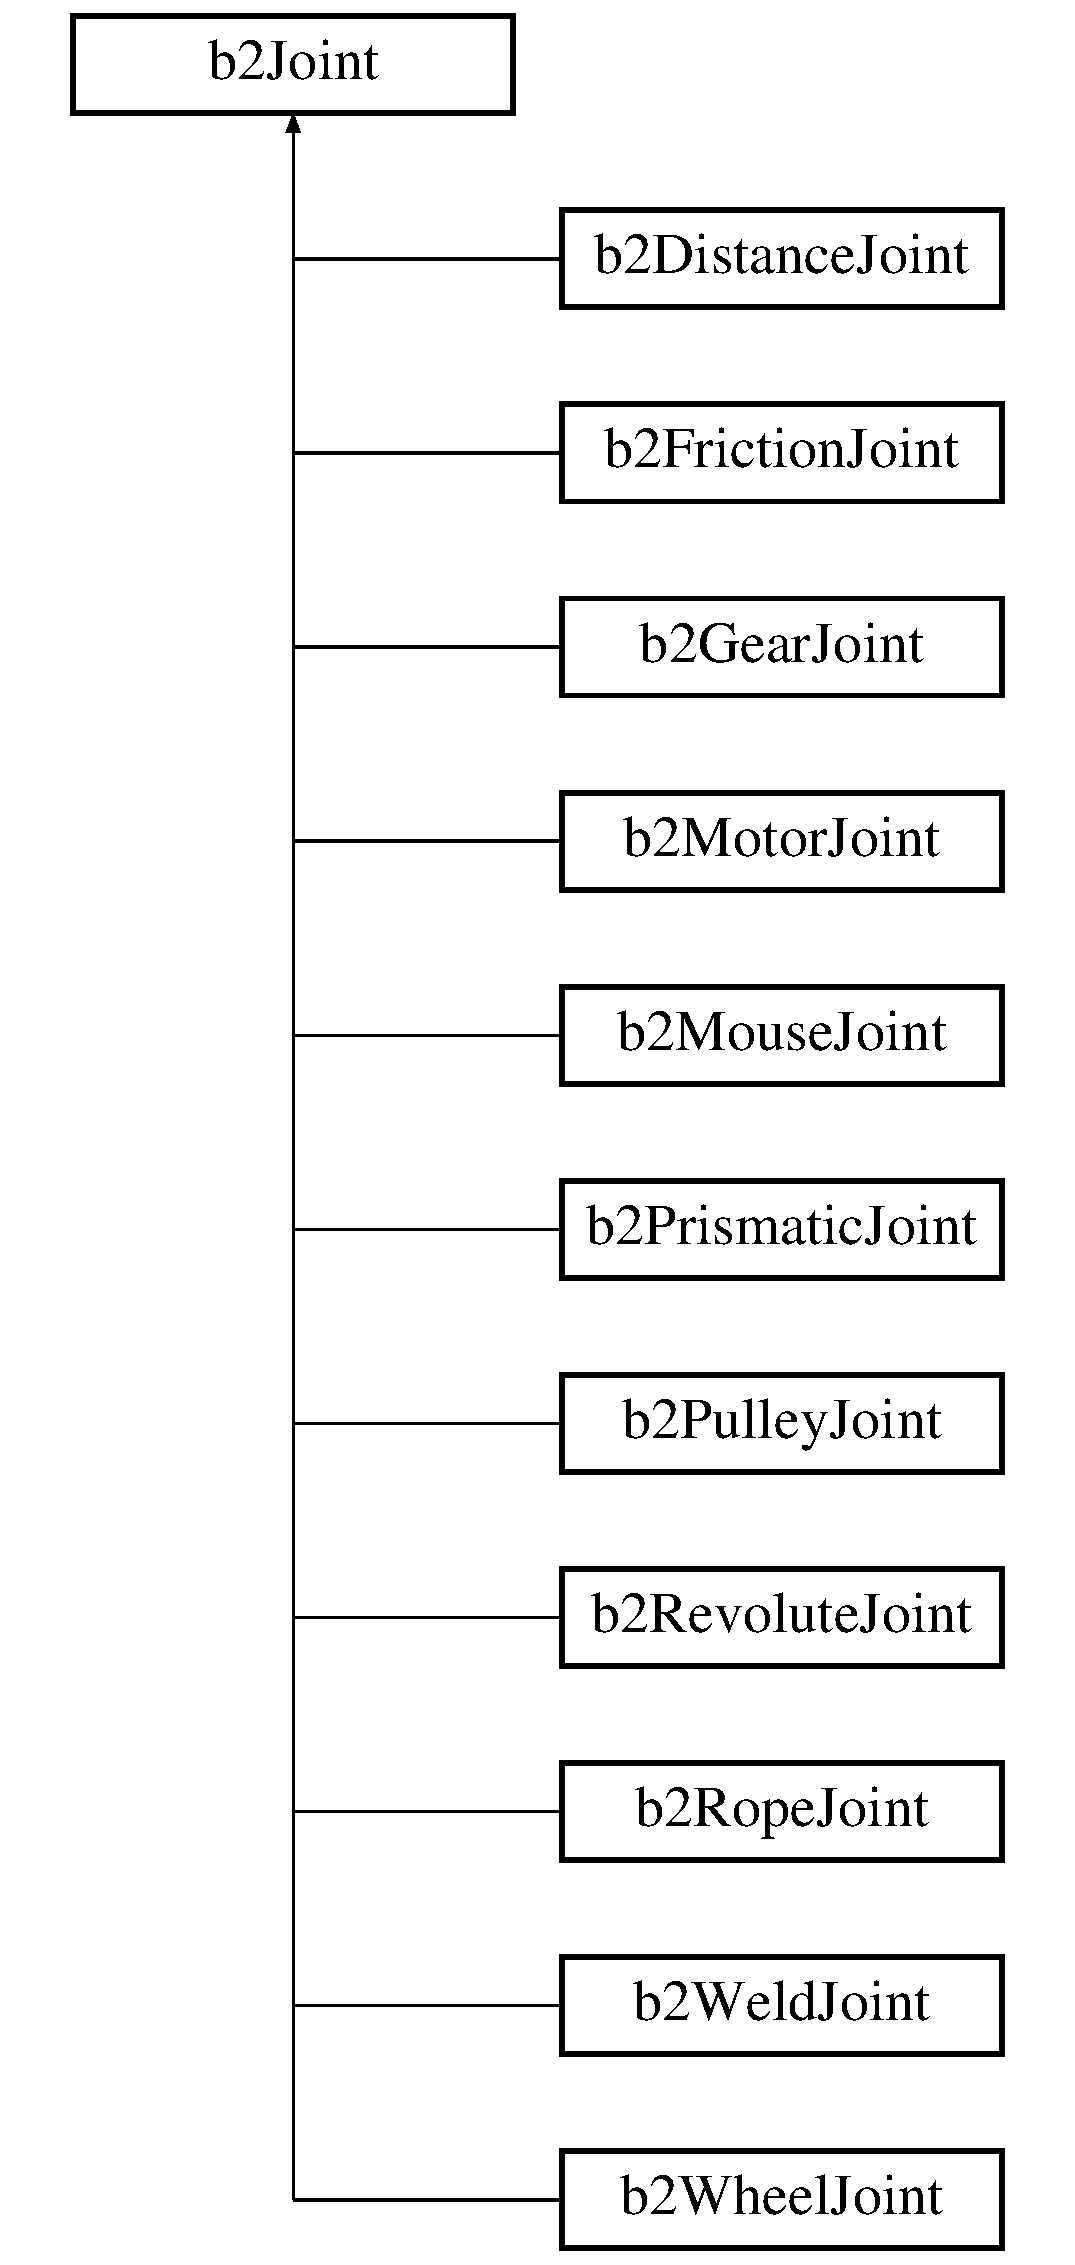
\includegraphics[height=12.000000cm]{classb2Joint}
\end{center}
\end{figure}
\subsection*{Public Member Functions}
\begin{DoxyCompactItemize}
\item 
\mbox{\Hypertarget{classb2Joint_ac56eef62fe1ac7c9e5e21a79fb035255}\label{classb2Joint_ac56eef62fe1ac7c9e5e21a79fb035255}} 
b2\+Joint\+Type \mbox{\hyperlink{classb2Joint_ac56eef62fe1ac7c9e5e21a79fb035255}{Get\+Type}} () const
\begin{DoxyCompactList}\small\item\em Get the type of the concrete joint. \end{DoxyCompactList}\item 
\mbox{\Hypertarget{classb2Joint_a2ed5eca3dbdce48665c14452b280613f}\label{classb2Joint_a2ed5eca3dbdce48665c14452b280613f}} 
\mbox{\hyperlink{classb2Body}{b2\+Body}} $\ast$ \mbox{\hyperlink{classb2Joint_a2ed5eca3dbdce48665c14452b280613f}{Get\+BodyA}} ()
\begin{DoxyCompactList}\small\item\em Get the first body attached to this joint. \end{DoxyCompactList}\item 
\mbox{\Hypertarget{classb2Joint_a700b3d4c87f34f456151b9598e4641a0}\label{classb2Joint_a700b3d4c87f34f456151b9598e4641a0}} 
\mbox{\hyperlink{classb2Body}{b2\+Body}} $\ast$ \mbox{\hyperlink{classb2Joint_a700b3d4c87f34f456151b9598e4641a0}{Get\+BodyB}} ()
\begin{DoxyCompactList}\small\item\em Get the second body attached to this joint. \end{DoxyCompactList}\item 
\mbox{\Hypertarget{classb2Joint_abe46ca3aad5db73909a9b5a7b2117447}\label{classb2Joint_abe46ca3aad5db73909a9b5a7b2117447}} 
virtual \mbox{\hyperlink{structb2Vec2}{b2\+Vec2}} \mbox{\hyperlink{classb2Joint_abe46ca3aad5db73909a9b5a7b2117447}{Get\+AnchorA}} () const =0
\begin{DoxyCompactList}\small\item\em Get the anchor point on bodyA in world coordinates. \end{DoxyCompactList}\item 
\mbox{\Hypertarget{classb2Joint_a88e947c65d4ea26fe539f02a8cb7f7a9}\label{classb2Joint_a88e947c65d4ea26fe539f02a8cb7f7a9}} 
virtual \mbox{\hyperlink{structb2Vec2}{b2\+Vec2}} \mbox{\hyperlink{classb2Joint_a88e947c65d4ea26fe539f02a8cb7f7a9}{Get\+AnchorB}} () const =0
\begin{DoxyCompactList}\small\item\em Get the anchor point on bodyB in world coordinates. \end{DoxyCompactList}\item 
\mbox{\Hypertarget{classb2Joint_a7e0eddefb9b69ad050b8ef6425838a74}\label{classb2Joint_a7e0eddefb9b69ad050b8ef6425838a74}} 
virtual \mbox{\hyperlink{structb2Vec2}{b2\+Vec2}} \mbox{\hyperlink{classb2Joint_a7e0eddefb9b69ad050b8ef6425838a74}{Get\+Reaction\+Force}} (float32 inv\+\_\+dt) const =0
\begin{DoxyCompactList}\small\item\em Get the reaction force on bodyB at the joint anchor in Newtons. \end{DoxyCompactList}\item 
\mbox{\Hypertarget{classb2Joint_ae355e441c2aa842777dc04e24f15ced0}\label{classb2Joint_ae355e441c2aa842777dc04e24f15ced0}} 
virtual float32 \mbox{\hyperlink{classb2Joint_ae355e441c2aa842777dc04e24f15ced0}{Get\+Reaction\+Torque}} (float32 inv\+\_\+dt) const =0
\begin{DoxyCompactList}\small\item\em Get the reaction torque on bodyB in N$\ast$m. \end{DoxyCompactList}\item 
\mbox{\Hypertarget{classb2Joint_a1a0e2137b631010750c728cb4e276e5d}\label{classb2Joint_a1a0e2137b631010750c728cb4e276e5d}} 
\mbox{\hyperlink{classb2Joint}{b2\+Joint}} $\ast$ \mbox{\hyperlink{classb2Joint_a1a0e2137b631010750c728cb4e276e5d}{Get\+Next}} ()
\begin{DoxyCompactList}\small\item\em Get the next joint the world joint list. \end{DoxyCompactList}\item 
\mbox{\Hypertarget{classb2Joint_aac18301414d6ca0a20aefb471c709e78}\label{classb2Joint_aac18301414d6ca0a20aefb471c709e78}} 
const \mbox{\hyperlink{classb2Joint}{b2\+Joint}} $\ast$ {\bfseries Get\+Next} () const
\item 
\mbox{\Hypertarget{classb2Joint_a798c593c7a4958d408bca10f3b3788f9}\label{classb2Joint_a798c593c7a4958d408bca10f3b3788f9}} 
void $\ast$ \mbox{\hyperlink{classb2Joint_a798c593c7a4958d408bca10f3b3788f9}{Get\+User\+Data}} () const
\begin{DoxyCompactList}\small\item\em Get the user data pointer. \end{DoxyCompactList}\item 
\mbox{\Hypertarget{classb2Joint_a492f2d02496437572aaec6013ebdc1c8}\label{classb2Joint_a492f2d02496437572aaec6013ebdc1c8}} 
void \mbox{\hyperlink{classb2Joint_a492f2d02496437572aaec6013ebdc1c8}{Set\+User\+Data}} (void $\ast$data)
\begin{DoxyCompactList}\small\item\em Set the user data pointer. \end{DoxyCompactList}\item 
\mbox{\Hypertarget{classb2Joint_ae9cfbd158216c9855c2f018ff3c9c922}\label{classb2Joint_ae9cfbd158216c9855c2f018ff3c9c922}} 
bool \mbox{\hyperlink{classb2Joint_ae9cfbd158216c9855c2f018ff3c9c922}{Is\+Active}} () const
\begin{DoxyCompactList}\small\item\em Short-\/cut function to determine if either body is inactive. \end{DoxyCompactList}\item 
bool \mbox{\hyperlink{classb2Joint_a48492903df96c8a7b8cad8ed826f8cb0}{Get\+Collide\+Connected}} () const
\item 
\mbox{\Hypertarget{classb2Joint_abd35e7316017ad9a40d5dbf9b5ba3f36}\label{classb2Joint_abd35e7316017ad9a40d5dbf9b5ba3f36}} 
virtual void \mbox{\hyperlink{classb2Joint_abd35e7316017ad9a40d5dbf9b5ba3f36}{Dump}} ()
\begin{DoxyCompactList}\small\item\em Dump this joint to the log file. \end{DoxyCompactList}\item 
\mbox{\Hypertarget{classb2Joint_a7804f649e993dc0fd9ae47fde5601f90}\label{classb2Joint_a7804f649e993dc0fd9ae47fde5601f90}} 
virtual void \mbox{\hyperlink{classb2Joint_a7804f649e993dc0fd9ae47fde5601f90}{Shift\+Origin}} (const \mbox{\hyperlink{structb2Vec2}{b2\+Vec2}} \&new\+Origin)
\begin{DoxyCompactList}\small\item\em Shift the origin for any points stored in world coordinates. \end{DoxyCompactList}\end{DoxyCompactItemize}
\subsection*{Protected Member Functions}
\begin{DoxyCompactItemize}
\item 
\mbox{\Hypertarget{classb2Joint_a8d6cce91546335fe95325d5e29c06a19}\label{classb2Joint_a8d6cce91546335fe95325d5e29c06a19}} 
{\bfseries b2\+Joint} (const \mbox{\hyperlink{structb2JointDef}{b2\+Joint\+Def}} $\ast$def)
\item 
\mbox{\Hypertarget{classb2Joint_a599c013de5514e02684b958b31dd76a4}\label{classb2Joint_a599c013de5514e02684b958b31dd76a4}} 
virtual void {\bfseries Init\+Velocity\+Constraints} (const \mbox{\hyperlink{structb2SolverData}{b2\+Solver\+Data}} \&data)=0
\item 
\mbox{\Hypertarget{classb2Joint_ad302c8d02efcfe934158de0dc429348d}\label{classb2Joint_ad302c8d02efcfe934158de0dc429348d}} 
virtual void {\bfseries Solve\+Velocity\+Constraints} (const \mbox{\hyperlink{structb2SolverData}{b2\+Solver\+Data}} \&data)=0
\item 
\mbox{\Hypertarget{classb2Joint_af767ac9aa494bd15cdf83dfe3e487d9c}\label{classb2Joint_af767ac9aa494bd15cdf83dfe3e487d9c}} 
virtual bool {\bfseries Solve\+Position\+Constraints} (const \mbox{\hyperlink{structb2SolverData}{b2\+Solver\+Data}} \&data)=0
\end{DoxyCompactItemize}
\subsection*{Static Protected Member Functions}
\begin{DoxyCompactItemize}
\item 
\mbox{\Hypertarget{classb2Joint_a2e500c93107d0bf6b0a21654528faeab}\label{classb2Joint_a2e500c93107d0bf6b0a21654528faeab}} 
static \mbox{\hyperlink{classb2Joint}{b2\+Joint}} $\ast$ {\bfseries Create} (const \mbox{\hyperlink{structb2JointDef}{b2\+Joint\+Def}} $\ast$def, \mbox{\hyperlink{classb2BlockAllocator}{b2\+Block\+Allocator}} $\ast$allocator)
\item 
\mbox{\Hypertarget{classb2Joint_acf52946b6672d77f268b849ccb09e003}\label{classb2Joint_acf52946b6672d77f268b849ccb09e003}} 
static void {\bfseries Destroy} (\mbox{\hyperlink{classb2Joint}{b2\+Joint}} $\ast$joint, \mbox{\hyperlink{classb2BlockAllocator}{b2\+Block\+Allocator}} $\ast$allocator)
\end{DoxyCompactItemize}
\subsection*{Protected Attributes}
\begin{DoxyCompactItemize}
\item 
\mbox{\Hypertarget{classb2Joint_a3fd3f2532d108d81df81427815210a59}\label{classb2Joint_a3fd3f2532d108d81df81427815210a59}} 
b2\+Joint\+Type {\bfseries m\+\_\+type}
\item 
\mbox{\Hypertarget{classb2Joint_a940166e7b5d87cec1ad0603e0388854a}\label{classb2Joint_a940166e7b5d87cec1ad0603e0388854a}} 
\mbox{\hyperlink{classb2Joint}{b2\+Joint}} $\ast$ {\bfseries m\+\_\+prev}
\item 
\mbox{\Hypertarget{classb2Joint_aad16778ba9c51cebb767ff7df6ed80b5}\label{classb2Joint_aad16778ba9c51cebb767ff7df6ed80b5}} 
\mbox{\hyperlink{classb2Joint}{b2\+Joint}} $\ast$ {\bfseries m\+\_\+next}
\item 
\mbox{\Hypertarget{classb2Joint_a406ea423db1fe6484408d73df647f7b2}\label{classb2Joint_a406ea423db1fe6484408d73df647f7b2}} 
\mbox{\hyperlink{structb2JointEdge}{b2\+Joint\+Edge}} {\bfseries m\+\_\+edgeA}
\item 
\mbox{\Hypertarget{classb2Joint_a1041219dcd353ea815ebd78f904af547}\label{classb2Joint_a1041219dcd353ea815ebd78f904af547}} 
\mbox{\hyperlink{structb2JointEdge}{b2\+Joint\+Edge}} {\bfseries m\+\_\+edgeB}
\item 
\mbox{\Hypertarget{classb2Joint_abaebb784a51abb7d66de302ba07a4467}\label{classb2Joint_abaebb784a51abb7d66de302ba07a4467}} 
\mbox{\hyperlink{classb2Body}{b2\+Body}} $\ast$ {\bfseries m\+\_\+bodyA}
\item 
\mbox{\Hypertarget{classb2Joint_a1fd77fcbcb8a8a3729c7dc5b790d7200}\label{classb2Joint_a1fd77fcbcb8a8a3729c7dc5b790d7200}} 
\mbox{\hyperlink{classb2Body}{b2\+Body}} $\ast$ {\bfseries m\+\_\+bodyB}
\item 
\mbox{\Hypertarget{classb2Joint_ae207295484bc040b6b52d96d63f1369f}\label{classb2Joint_ae207295484bc040b6b52d96d63f1369f}} 
int32 {\bfseries m\+\_\+index}
\item 
\mbox{\Hypertarget{classb2Joint_a777e45428d9a74d626f4afa1b45e1975}\label{classb2Joint_a777e45428d9a74d626f4afa1b45e1975}} 
bool {\bfseries m\+\_\+island\+Flag}
\item 
\mbox{\Hypertarget{classb2Joint_ac1a93c14c8dd666bb487db6c98daad33}\label{classb2Joint_ac1a93c14c8dd666bb487db6c98daad33}} 
bool {\bfseries m\+\_\+collide\+Connected}
\item 
\mbox{\Hypertarget{classb2Joint_ae8a31b6d5d6e76ccf7c975b2b3ae7366}\label{classb2Joint_ae8a31b6d5d6e76ccf7c975b2b3ae7366}} 
void $\ast$ {\bfseries m\+\_\+user\+Data}
\end{DoxyCompactItemize}
\subsection*{Friends}
\begin{DoxyCompactItemize}
\item 
\mbox{\Hypertarget{classb2Joint_a4bd536c5a7c0587913765bbc2693ceea}\label{classb2Joint_a4bd536c5a7c0587913765bbc2693ceea}} 
class {\bfseries b2\+World}
\item 
\mbox{\Hypertarget{classb2Joint_a010ab52de250e5fe30a45d642f46405b}\label{classb2Joint_a010ab52de250e5fe30a45d642f46405b}} 
class {\bfseries b2\+Body}
\item 
\mbox{\Hypertarget{classb2Joint_afc682950b8c4f251804fc1938663098b}\label{classb2Joint_afc682950b8c4f251804fc1938663098b}} 
class {\bfseries b2\+Island}
\item 
\mbox{\Hypertarget{classb2Joint_a13c275221e30bb485e17e4e04553cb71}\label{classb2Joint_a13c275221e30bb485e17e4e04553cb71}} 
class {\bfseries b2\+Gear\+Joint}
\end{DoxyCompactItemize}


\subsection{Detailed Description}
The base joint class. Joints are used to constraint two bodies together in various fashions. Some joints also feature limits and motors. 

\subsection{Member Function Documentation}
\mbox{\Hypertarget{classb2Joint_a48492903df96c8a7b8cad8ed826f8cb0}\label{classb2Joint_a48492903df96c8a7b8cad8ed826f8cb0}} 
\index{b2\+Joint@{b2\+Joint}!Get\+Collide\+Connected@{Get\+Collide\+Connected}}
\index{Get\+Collide\+Connected@{Get\+Collide\+Connected}!b2\+Joint@{b2\+Joint}}
\subsubsection{\texorpdfstring{Get\+Collide\+Connected()}{GetCollideConnected()}}
{\footnotesize\ttfamily bool b2\+Joint\+::\+Get\+Collide\+Connected (\begin{DoxyParamCaption}{ }\end{DoxyParamCaption}) const\hspace{0.3cm}{\ttfamily [inline]}}

Get collide connected. Note\+: modifying the collide connect flag won\textquotesingle{}t work correctly because the flag is only checked when fixture A\+A\+B\+Bs begin to overlap. 

The documentation for this class was generated from the following files\+:\begin{DoxyCompactItemize}
\item 
Dynamics/\+Joints/b2\+Joint.\+h\item 
Dynamics/\+Joints/b2\+Joint.\+cpp\end{DoxyCompactItemize}

\hypertarget{structb2JointDef}{}\section{b2\+Joint\+Def Struct Reference}
\label{structb2JointDef}\index{b2\+Joint\+Def@{b2\+Joint\+Def}}


Joint definitions are used to construct joints.  




{\ttfamily \#include $<$b2\+Joint.\+h$>$}

Inheritance diagram for b2\+Joint\+Def\+:\begin{figure}[H]
\begin{center}
\leavevmode
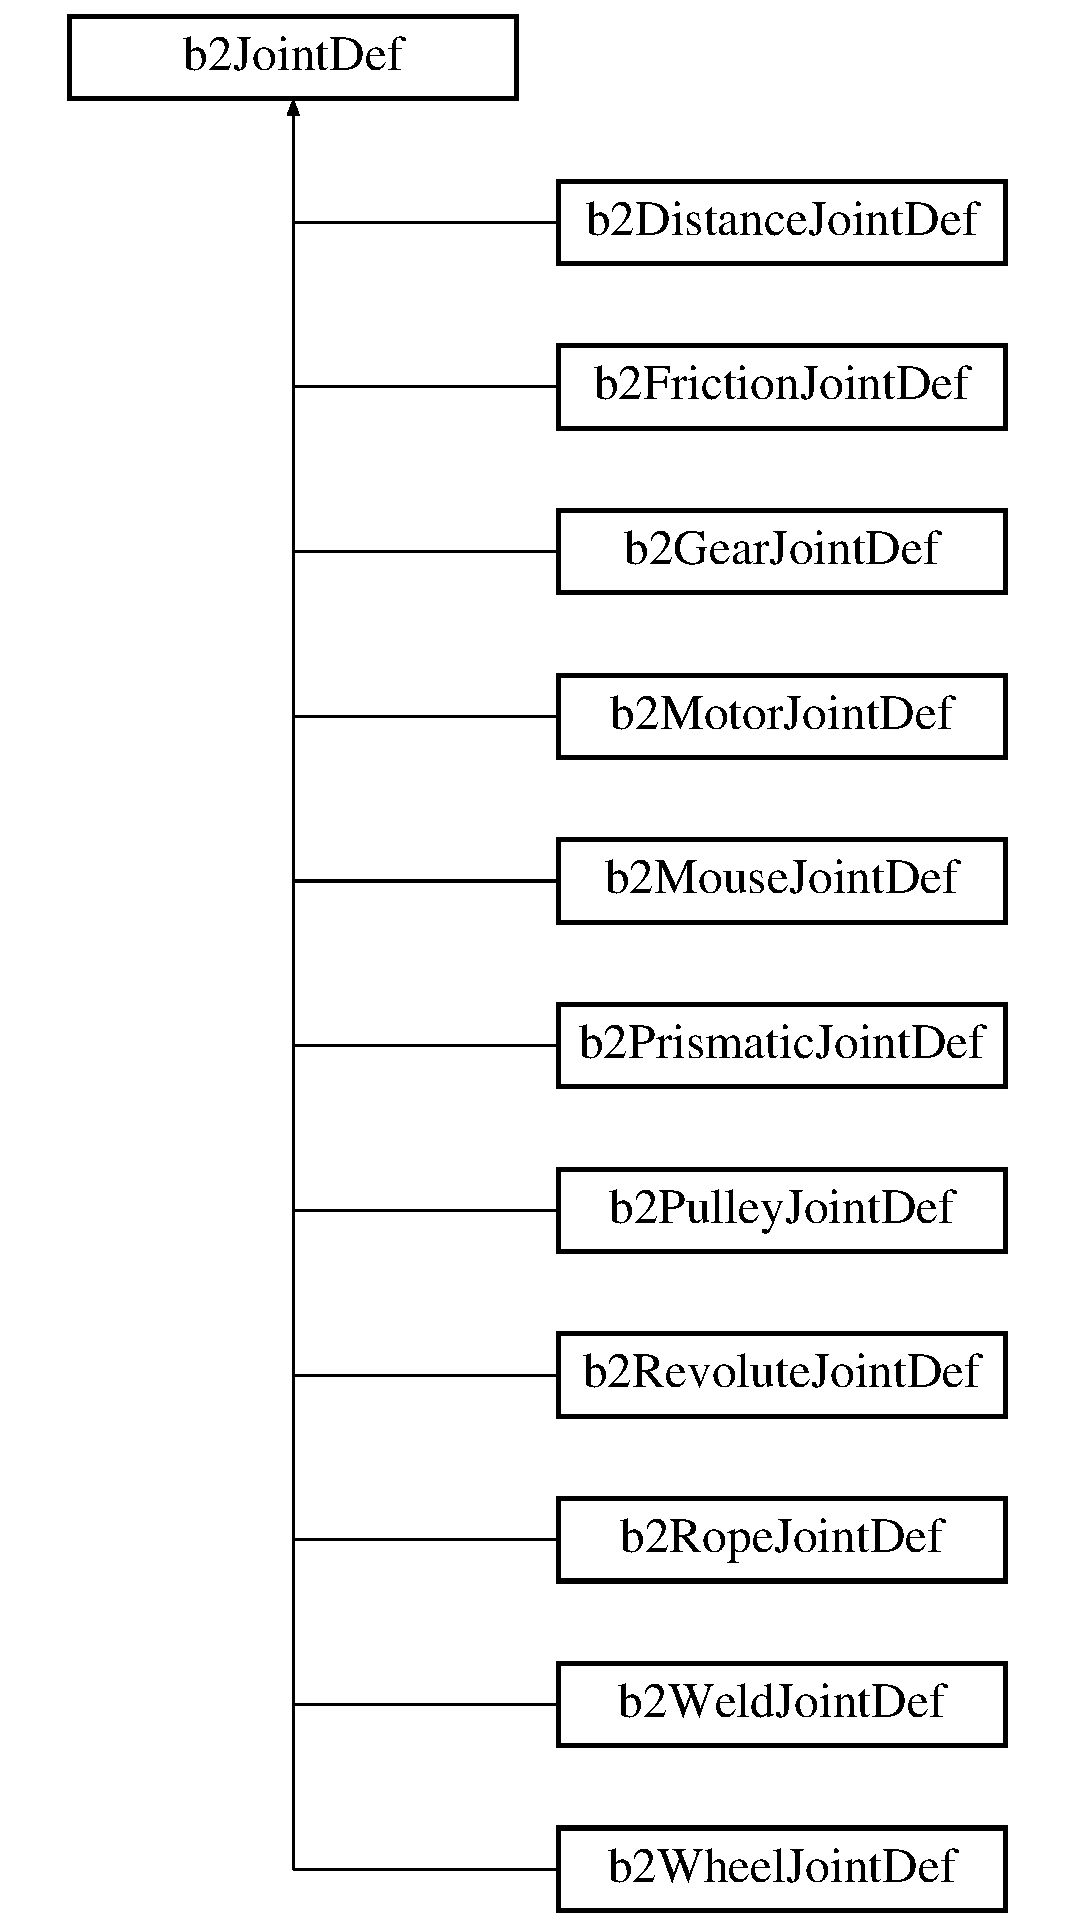
\includegraphics[height=12.000000cm]{structb2JointDef}
\end{center}
\end{figure}
\subsection*{Public Attributes}
\begin{DoxyCompactItemize}
\item 
\mbox{\Hypertarget{structb2JointDef_a470f2879b24adb05facbd49f338856fb}\label{structb2JointDef_a470f2879b24adb05facbd49f338856fb}} 
b2\+Joint\+Type \mbox{\hyperlink{structb2JointDef_a470f2879b24adb05facbd49f338856fb}{type}}
\begin{DoxyCompactList}\small\item\em The joint type is set automatically for concrete joint types. \end{DoxyCompactList}\item 
\mbox{\Hypertarget{structb2JointDef_a07eb150daaaa52fc09c3bcf402b295fe}\label{structb2JointDef_a07eb150daaaa52fc09c3bcf402b295fe}} 
void $\ast$ \mbox{\hyperlink{structb2JointDef_a07eb150daaaa52fc09c3bcf402b295fe}{user\+Data}}
\begin{DoxyCompactList}\small\item\em Use this to attach application specific data to your joints. \end{DoxyCompactList}\item 
\mbox{\Hypertarget{structb2JointDef_a8cd54c93da396be75a9788f2c6897f05}\label{structb2JointDef_a8cd54c93da396be75a9788f2c6897f05}} 
\mbox{\hyperlink{classb2Body}{b2\+Body}} $\ast$ \mbox{\hyperlink{structb2JointDef_a8cd54c93da396be75a9788f2c6897f05}{bodyA}}
\begin{DoxyCompactList}\small\item\em The first attached body. \end{DoxyCompactList}\item 
\mbox{\Hypertarget{structb2JointDef_aa4f4dee2fbcd12187b19506b60e68e3d}\label{structb2JointDef_aa4f4dee2fbcd12187b19506b60e68e3d}} 
\mbox{\hyperlink{classb2Body}{b2\+Body}} $\ast$ \mbox{\hyperlink{structb2JointDef_aa4f4dee2fbcd12187b19506b60e68e3d}{bodyB}}
\begin{DoxyCompactList}\small\item\em The second attached body. \end{DoxyCompactList}\item 
\mbox{\Hypertarget{structb2JointDef_aef099a1f89b64e230173b6016848ea9b}\label{structb2JointDef_aef099a1f89b64e230173b6016848ea9b}} 
bool \mbox{\hyperlink{structb2JointDef_aef099a1f89b64e230173b6016848ea9b}{collide\+Connected}}
\begin{DoxyCompactList}\small\item\em Set this flag to true if the attached bodies should collide. \end{DoxyCompactList}\end{DoxyCompactItemize}


\subsection{Detailed Description}
Joint definitions are used to construct joints. 

The documentation for this struct was generated from the following file\+:\begin{DoxyCompactItemize}
\item 
Dynamics/\+Joints/b2\+Joint.\+h\end{DoxyCompactItemize}

\hypertarget{structb2JointEdge}{}\section{b2\+Joint\+Edge Struct Reference}
\label{structb2JointEdge}\index{b2\+Joint\+Edge@{b2\+Joint\+Edge}}


{\ttfamily \#include $<$b2\+Joint.\+h$>$}

\subsection*{Public Attributes}
\begin{DoxyCompactItemize}
\item 
\mbox{\Hypertarget{structb2JointEdge_a64aef21fb91211871de8796baecccb95}\label{structb2JointEdge_a64aef21fb91211871de8796baecccb95}} 
\mbox{\hyperlink{classb2Body}{b2\+Body}} $\ast$ \mbox{\hyperlink{structb2JointEdge_a64aef21fb91211871de8796baecccb95}{other}}
\begin{DoxyCompactList}\small\item\em provides quick access to the other body attached. \end{DoxyCompactList}\item 
\mbox{\Hypertarget{structb2JointEdge_ab5bac5d495af1280c50271f56a221503}\label{structb2JointEdge_ab5bac5d495af1280c50271f56a221503}} 
\mbox{\hyperlink{classb2Joint}{b2\+Joint}} $\ast$ \mbox{\hyperlink{structb2JointEdge_ab5bac5d495af1280c50271f56a221503}{joint}}
\begin{DoxyCompactList}\small\item\em the joint \end{DoxyCompactList}\item 
\mbox{\Hypertarget{structb2JointEdge_acc3621e38d9664db2805e0fc29d71335}\label{structb2JointEdge_acc3621e38d9664db2805e0fc29d71335}} 
\mbox{\hyperlink{structb2JointEdge}{b2\+Joint\+Edge}} $\ast$ \mbox{\hyperlink{structb2JointEdge_acc3621e38d9664db2805e0fc29d71335}{prev}}
\begin{DoxyCompactList}\small\item\em the previous joint edge in the body\textquotesingle{}s joint list \end{DoxyCompactList}\item 
\mbox{\Hypertarget{structb2JointEdge_a3d17286bc697bb620ee151e4cd07438c}\label{structb2JointEdge_a3d17286bc697bb620ee151e4cd07438c}} 
\mbox{\hyperlink{structb2JointEdge}{b2\+Joint\+Edge}} $\ast$ \mbox{\hyperlink{structb2JointEdge_a3d17286bc697bb620ee151e4cd07438c}{next}}
\begin{DoxyCompactList}\small\item\em the next joint edge in the body\textquotesingle{}s joint list \end{DoxyCompactList}\end{DoxyCompactItemize}


\subsection{Detailed Description}
A joint edge is used to connect bodies and joints together in a joint graph where each body is a node and each joint is an edge. A joint edge belongs to a doubly linked list maintained in each attached _body. Each joint has two joint nodes, one for each attached _body.

The documentation for this struct was generated from the following file\+:\begin{DoxyCompactItemize}
\item 
Dynamics/\+Joints/b2\+Joint.\+h\end{DoxyCompactItemize}

\hypertarget{structb2Manifold}{}\section{b2\+Manifold Struct Reference}
\label{structb2Manifold}\index{b2\+Manifold@{b2\+Manifold}}


{\ttfamily \#include $<$b2\+Collision.\+h$>$}

\subsection*{Public Types}
\begin{DoxyCompactItemize}
\item 
\mbox{\Hypertarget{structb2Manifold_aa9c347e2ff2e27ee820a926efbb33e12}\label{structb2Manifold_aa9c347e2ff2e27ee820a926efbb33e12}} 
enum {\bfseries Type} \{ {\bfseries e\+\_\+circles}, 
{\bfseries e\+\_\+faceA}, 
{\bfseries e\+\_\+faceB}
 \}
\end{DoxyCompactItemize}
\subsection*{Public Attributes}
\begin{DoxyCompactItemize}
\item 
\mbox{\Hypertarget{structb2Manifold_ab8021128e9792cc7391a8804ea02173d}\label{structb2Manifold_ab8021128e9792cc7391a8804ea02173d}} 
\mbox{\hyperlink{structb2ManifoldPoint}{b2\+Manifold\+Point}} \mbox{\hyperlink{structb2Manifold_ab8021128e9792cc7391a8804ea02173d}{points}} \mbox{[}\mbox{\hyperlink{b2Settings_8h_aa5f44cc9edf711433dea2b2ec94f3c42}{b2\+\_\+max\+Manifold\+Points}}\mbox{]}
\begin{DoxyCompactList}\small\item\em the points of contact \end{DoxyCompactList}\item 
\mbox{\Hypertarget{structb2Manifold_a3604e9fef2a03347c5649c71a9fd4c79}\label{structb2Manifold_a3604e9fef2a03347c5649c71a9fd4c79}} 
\mbox{\hyperlink{structb2Vec2}{b2\+Vec2}} \mbox{\hyperlink{structb2Manifold_a3604e9fef2a03347c5649c71a9fd4c79}{local\+Normal}}
\begin{DoxyCompactList}\small\item\em not use for Type\+::e\+\_\+points \end{DoxyCompactList}\item 
\mbox{\Hypertarget{structb2Manifold_a8825cea31b27dbbaf22c13c3070870d5}\label{structb2Manifold_a8825cea31b27dbbaf22c13c3070870d5}} 
\mbox{\hyperlink{structb2Vec2}{b2\+Vec2}} \mbox{\hyperlink{structb2Manifold_a8825cea31b27dbbaf22c13c3070870d5}{local\+Point}}
\begin{DoxyCompactList}\small\item\em usage depends on manifold type \end{DoxyCompactList}\item 
\mbox{\Hypertarget{structb2Manifold_a4cb6ceba7105513b1e5bd6dbf0cce168}\label{structb2Manifold_a4cb6ceba7105513b1e5bd6dbf0cce168}} 
Type {\bfseries type}
\item 
\mbox{\Hypertarget{structb2Manifold_abf59ff6fa36bed34b0242ad54951a696}\label{structb2Manifold_abf59ff6fa36bed34b0242ad54951a696}} 
int32 \mbox{\hyperlink{structb2Manifold_abf59ff6fa36bed34b0242ad54951a696}{point\+Count}}
\begin{DoxyCompactList}\small\item\em the number of manifold points \end{DoxyCompactList}\end{DoxyCompactItemize}


\subsection{Detailed Description}
A manifold for two touching convex shapes. Box2D supports multiple types of contact\+:
\begin{DoxyItemize}
\item clip point versus plane with radius
\item point versus point with radius (circles) The local point usage depends on the manifold type\+: -\/e\+\_\+circles\+: the local center of circleA -\/e\+\_\+faceA\+: the center of faceA -\/e\+\_\+faceB\+: the center of faceB Similarly the local normal usage\+: -\/e\+\_\+circles\+: not used -\/e\+\_\+faceA\+: the normal on polygonA -\/e\+\_\+faceB\+: the normal on polygonB We store contacts in this way so that position correction can account for movement, which is critical for continuous physics. All contact scenarios must be expressed in one of these types. This structure is stored across time steps, so we keep it small. 
\end{DoxyItemize}

The documentation for this struct was generated from the following file\+:\begin{DoxyCompactItemize}
\item 
Collision/\mbox{\hyperlink{b2Collision_8h}{b2\+Collision.\+h}}\end{DoxyCompactItemize}

\hypertarget{structb2ManifoldPoint}{}\section{b2\+Manifold\+Point Struct Reference}
\label{structb2ManifoldPoint}\index{b2\+Manifold\+Point@{b2\+Manifold\+Point}}


{\ttfamily \#include $<$b2\+Collision.\+h$>$}

\subsection*{Public Attributes}
\begin{DoxyCompactItemize}
\item 
\mbox{\Hypertarget{structb2ManifoldPoint_ab3616990e7d1644deeeb691246094bfa}\label{structb2ManifoldPoint_ab3616990e7d1644deeeb691246094bfa}} 
\mbox{\hyperlink{structb2Vec2}{b2\+Vec2}} \mbox{\hyperlink{structb2ManifoldPoint_ab3616990e7d1644deeeb691246094bfa}{local\+Point}}
\begin{DoxyCompactList}\small\item\em usage depends on manifold type \end{DoxyCompactList}\item 
\mbox{\Hypertarget{structb2ManifoldPoint_af4218c2359cb7762cd4e9d8ecefab173}\label{structb2ManifoldPoint_af4218c2359cb7762cd4e9d8ecefab173}} 
float32 \mbox{\hyperlink{structb2ManifoldPoint_af4218c2359cb7762cd4e9d8ecefab173}{normal\+Impulse}}
\begin{DoxyCompactList}\small\item\em the non-\/penetration impulse \end{DoxyCompactList}\item 
\mbox{\Hypertarget{structb2ManifoldPoint_a0ac5375b1fc4675a0073129f56aa62c9}\label{structb2ManifoldPoint_a0ac5375b1fc4675a0073129f56aa62c9}} 
float32 \mbox{\hyperlink{structb2ManifoldPoint_a0ac5375b1fc4675a0073129f56aa62c9}{tangent\+Impulse}}
\begin{DoxyCompactList}\small\item\em the friction impulse \end{DoxyCompactList}\item 
\mbox{\Hypertarget{structb2ManifoldPoint_afa7ec272b2b27abe129540f8fbe57fc5}\label{structb2ManifoldPoint_afa7ec272b2b27abe129540f8fbe57fc5}} 
\mbox{\hyperlink{unionb2ContactID}{b2\+Contact\+ID}} \mbox{\hyperlink{structb2ManifoldPoint_afa7ec272b2b27abe129540f8fbe57fc5}{id}}
\begin{DoxyCompactList}\small\item\em uniquely identifies a contact point between two shapes \end{DoxyCompactList}\end{DoxyCompactItemize}


\subsection{Detailed Description}
A manifold point is a contact point belonging to a contact manifold. It holds details related to the geometry and dynamics of the contact points. The local point usage depends on the manifold type\+: -\/e\+\_\+circles\+: the local center of circleB -\/e\+\_\+faceA\+: the local center of cirlceB or the clip point of polygonB -\/e\+\_\+faceB\+: the clip point of polygonA This structure is stored across time steps, so we keep it small. Note\+: the impulses are used for internal caching and may not provide reliable contact forces, especially for high speed collisions. 

The documentation for this struct was generated from the following file\+:\begin{DoxyCompactItemize}
\item 
Collision/\mbox{\hyperlink{b2Collision_8h}{b2\+Collision.\+h}}\end{DoxyCompactItemize}

\hypertarget{structb2MassData}{}\section{b2\+Mass\+Data Struct Reference}
\label{structb2MassData}\index{b2\+Mass\+Data@{b2\+Mass\+Data}}


This holds the mass data computed for a shape.  




{\ttfamily \#include $<$b2\+Shape.\+h$>$}

\subsection*{Public Attributes}
\begin{DoxyCompactItemize}
\item 
\mbox{\Hypertarget{structb2MassData_aea85d9595a38d2eed05b8d2ea80d97b1}\label{structb2MassData_aea85d9595a38d2eed05b8d2ea80d97b1}} 
float32 \mbox{\hyperlink{structb2MassData_aea85d9595a38d2eed05b8d2ea80d97b1}{mass}}
\begin{DoxyCompactList}\small\item\em The mass of the shape, usually in kilograms. \end{DoxyCompactList}\item 
\mbox{\Hypertarget{structb2MassData_a1d59bebc7030c4dded0c2febc57ebdd7}\label{structb2MassData_a1d59bebc7030c4dded0c2febc57ebdd7}} 
\mbox{\hyperlink{structb2Vec2}{b2\+Vec2}} \mbox{\hyperlink{structb2MassData_a1d59bebc7030c4dded0c2febc57ebdd7}{center}}
\begin{DoxyCompactList}\small\item\em The position of the shape\textquotesingle{}s centroid relative to the shape\textquotesingle{}s origin. \end{DoxyCompactList}\item 
\mbox{\Hypertarget{structb2MassData_ad2d06e96e2d79d895df16ae0e5fe0376}\label{structb2MassData_ad2d06e96e2d79d895df16ae0e5fe0376}} 
float32 \mbox{\hyperlink{structb2MassData_ad2d06e96e2d79d895df16ae0e5fe0376}{I}}
\begin{DoxyCompactList}\small\item\em The rotational inertia of the shape about the local origin. \end{DoxyCompactList}\end{DoxyCompactItemize}


\subsection{Detailed Description}
This holds the mass data computed for a shape. 

The documentation for this struct was generated from the following file\+:\begin{DoxyCompactItemize}
\item 
Collision/\+Shapes/b2\+Shape.\+h\end{DoxyCompactItemize}

\hypertarget{structb2Mat22}{}\section{b2\+Mat22 Struct Reference}
\label{structb2Mat22}\index{b2\+Mat22@{b2\+Mat22}}


A 2-\/by-\/2 matrix. Stored in column-\/major order.  




{\ttfamily \#include $<$b2\+Math.\+h$>$}

\subsection*{Public Member Functions}
\begin{DoxyCompactItemize}
\item 
\mbox{\Hypertarget{structb2Mat22_ac3e10f6d457c8dab9062ba378f66bc4d}\label{structb2Mat22_ac3e10f6d457c8dab9062ba378f66bc4d}} 
\mbox{\hyperlink{structb2Mat22_ac3e10f6d457c8dab9062ba378f66bc4d}{b2\+Mat22}} ()
\begin{DoxyCompactList}\small\item\em The default constructor does nothing (for performance). \end{DoxyCompactList}\item 
\mbox{\Hypertarget{structb2Mat22_abd674c6d92e26962977f34bcd92ff24d}\label{structb2Mat22_abd674c6d92e26962977f34bcd92ff24d}} 
\mbox{\hyperlink{structb2Mat22_abd674c6d92e26962977f34bcd92ff24d}{b2\+Mat22}} (const \mbox{\hyperlink{structb2Vec2}{b2\+Vec2}} \&c1, const \mbox{\hyperlink{structb2Vec2}{b2\+Vec2}} \&c2)
\begin{DoxyCompactList}\small\item\em Construct this matrix using columns. \end{DoxyCompactList}\item 
\mbox{\Hypertarget{structb2Mat22_a41d5d8743bda32cb8c6e212528934810}\label{structb2Mat22_a41d5d8743bda32cb8c6e212528934810}} 
\mbox{\hyperlink{structb2Mat22_a41d5d8743bda32cb8c6e212528934810}{b2\+Mat22}} (float32 a11, float32 a12, float32 a21, float32 a22)
\begin{DoxyCompactList}\small\item\em Construct this matrix using scalars. \end{DoxyCompactList}\item 
\mbox{\Hypertarget{structb2Mat22_aed3bee1de38a0b3f36e21c90faa24112}\label{structb2Mat22_aed3bee1de38a0b3f36e21c90faa24112}} 
void \mbox{\hyperlink{structb2Mat22_aed3bee1de38a0b3f36e21c90faa24112}{Set}} (const \mbox{\hyperlink{structb2Vec2}{b2\+Vec2}} \&c1, const \mbox{\hyperlink{structb2Vec2}{b2\+Vec2}} \&c2)
\begin{DoxyCompactList}\small\item\em Initialize this matrix using columns. \end{DoxyCompactList}\item 
\mbox{\Hypertarget{structb2Mat22_a7192f063b771ac9ded060e41df890509}\label{structb2Mat22_a7192f063b771ac9ded060e41df890509}} 
void \mbox{\hyperlink{structb2Mat22_a7192f063b771ac9ded060e41df890509}{Set\+Identity}} ()
\begin{DoxyCompactList}\small\item\em Set this to the identity matrix. \end{DoxyCompactList}\item 
\mbox{\Hypertarget{structb2Mat22_aaeae95f61cf3171ffb94703980e3594b}\label{structb2Mat22_aaeae95f61cf3171ffb94703980e3594b}} 
void \mbox{\hyperlink{structb2Mat22_aaeae95f61cf3171ffb94703980e3594b}{Set\+Zero}} ()
\begin{DoxyCompactList}\small\item\em Set this matrix to all zeros. \end{DoxyCompactList}\item 
\mbox{\Hypertarget{structb2Mat22_ad0b0676deea081b761c67be48e0ac850}\label{structb2Mat22_ad0b0676deea081b761c67be48e0ac850}} 
\mbox{\hyperlink{structb2Mat22}{b2\+Mat22}} {\bfseries Get\+Inverse} () const
\item 
\mbox{\hyperlink{structb2Vec2}{b2\+Vec2}} \mbox{\hyperlink{structb2Mat22_a3313c8d135c01fbf74e7fea31f1ea4c1}{Solve}} (const \mbox{\hyperlink{structb2Vec2}{b2\+Vec2}} \&b) const
\end{DoxyCompactItemize}
\subsection*{Public Attributes}
\begin{DoxyCompactItemize}
\item 
\mbox{\Hypertarget{structb2Mat22_abaffa5fc1d401ea36415acffa6205689}\label{structb2Mat22_abaffa5fc1d401ea36415acffa6205689}} 
\mbox{\hyperlink{structb2Vec2}{b2\+Vec2}} {\bfseries ex}
\item 
\mbox{\Hypertarget{structb2Mat22_af19db58941d2cd146325ef3191b776fd}\label{structb2Mat22_af19db58941d2cd146325ef3191b776fd}} 
\mbox{\hyperlink{structb2Vec2}{b2\+Vec2}} {\bfseries ey}
\end{DoxyCompactItemize}


\subsection{Detailed Description}
A 2-\/by-\/2 matrix. Stored in column-\/major order. 

\subsection{Member Function Documentation}
\mbox{\Hypertarget{structb2Mat22_a3313c8d135c01fbf74e7fea31f1ea4c1}\label{structb2Mat22_a3313c8d135c01fbf74e7fea31f1ea4c1}} 
\index{b2\+Mat22@{b2\+Mat22}!Solve@{Solve}}
\index{Solve@{Solve}!b2\+Mat22@{b2\+Mat22}}
\subsubsection{\texorpdfstring{Solve()}{Solve()}}
{\footnotesize\ttfamily \mbox{\hyperlink{structb2Vec2}{b2\+Vec2}} b2\+Mat22\+::\+Solve (\begin{DoxyParamCaption}\item[{const \mbox{\hyperlink{structb2Vec2}{b2\+Vec2}} \&}]{b }\end{DoxyParamCaption}) const\hspace{0.3cm}{\ttfamily [inline]}}

Solve A $\ast$ x = b, where b is a column vector. This is more efficient than computing the inverse in one-\/shot cases. 

The documentation for this struct was generated from the following file\+:\begin{DoxyCompactItemize}
\item 
Common/b2\+Math.\+h\end{DoxyCompactItemize}

\hypertarget{structb2Mat33}{}\section{b2\+Mat33 Struct Reference}
\label{structb2Mat33}\index{b2\+Mat33@{b2\+Mat33}}


A 3-\/by-\/3 matrix. Stored in column-\/major order.  




{\ttfamily \#include $<$b2\+Math.\+h$>$}

\subsection*{Public Member Functions}
\begin{DoxyCompactItemize}
\item 
\mbox{\Hypertarget{structb2Mat33_a1f4d7ddf1c8a202fc08ec64dfe191463}\label{structb2Mat33_a1f4d7ddf1c8a202fc08ec64dfe191463}} 
\mbox{\hyperlink{structb2Mat33_a1f4d7ddf1c8a202fc08ec64dfe191463}{b2\+Mat33}} ()
\begin{DoxyCompactList}\small\item\em The default constructor does nothing (for performance). \end{DoxyCompactList}\item 
\mbox{\Hypertarget{structb2Mat33_a36d99a037008776c8d09fe0aeb5c759c}\label{structb2Mat33_a36d99a037008776c8d09fe0aeb5c759c}} 
\mbox{\hyperlink{structb2Mat33_a36d99a037008776c8d09fe0aeb5c759c}{b2\+Mat33}} (const \mbox{\hyperlink{structb2Vec3}{b2\+Vec3}} \&c1, const \mbox{\hyperlink{structb2Vec3}{b2\+Vec3}} \&c2, const \mbox{\hyperlink{structb2Vec3}{b2\+Vec3}} \&c3)
\begin{DoxyCompactList}\small\item\em Construct this matrix using columns. \end{DoxyCompactList}\item 
\mbox{\Hypertarget{structb2Mat33_a42fc6953b025e1c8b59717d0ee7accde}\label{structb2Mat33_a42fc6953b025e1c8b59717d0ee7accde}} 
void \mbox{\hyperlink{structb2Mat33_a42fc6953b025e1c8b59717d0ee7accde}{Set\+Zero}} ()
\begin{DoxyCompactList}\small\item\em Set this matrix to all zeros. \end{DoxyCompactList}\item 
\mbox{\hyperlink{structb2Vec3}{b2\+Vec3}} \mbox{\hyperlink{structb2Mat33_a2ce48f409ba5951a04da821dada9e285}{Solve33}} (const \mbox{\hyperlink{structb2Vec3}{b2\+Vec3}} \&b) const
\item 
\mbox{\hyperlink{structb2Vec2}{b2\+Vec2}} \mbox{\hyperlink{structb2Mat33_acdf892aab7e26283f8aa600ade91dcef}{Solve22}} (const \mbox{\hyperlink{structb2Vec2}{b2\+Vec2}} \&b) const
\item 
void \mbox{\hyperlink{structb2Mat33_aa020bfd08e28c4cecda303ba335fe517}{Get\+Inverse22}} (\mbox{\hyperlink{structb2Mat33}{b2\+Mat33}} $\ast$M) const
\item 
void \mbox{\hyperlink{structb2Mat33_a2620944663233096d3b82bc4b1a991e9}{Get\+Sym\+Inverse33}} (\mbox{\hyperlink{structb2Mat33}{b2\+Mat33}} $\ast$M) const
\begin{DoxyCompactList}\small\item\em Returns the zero matrix if singular. \end{DoxyCompactList}\end{DoxyCompactItemize}
\subsection*{Public Attributes}
\begin{DoxyCompactItemize}
\item 
\mbox{\Hypertarget{structb2Mat33_a132f00e6550d1e19c75fb60ce1229638}\label{structb2Mat33_a132f00e6550d1e19c75fb60ce1229638}} 
\mbox{\hyperlink{structb2Vec3}{b2\+Vec3}} {\bfseries ex}
\item 
\mbox{\Hypertarget{structb2Mat33_ababc69c718c73a04a651f7a6a981ecf4}\label{structb2Mat33_ababc69c718c73a04a651f7a6a981ecf4}} 
\mbox{\hyperlink{structb2Vec3}{b2\+Vec3}} {\bfseries ey}
\item 
\mbox{\Hypertarget{structb2Mat33_ae700fc46f679b4ef211a2517005b0557}\label{structb2Mat33_ae700fc46f679b4ef211a2517005b0557}} 
\mbox{\hyperlink{structb2Vec3}{b2\+Vec3}} {\bfseries ez}
\end{DoxyCompactItemize}


\subsection{Detailed Description}
A 3-\/by-\/3 matrix. Stored in column-\/major order. 

\subsection{Member Function Documentation}
\mbox{\Hypertarget{structb2Mat33_aa020bfd08e28c4cecda303ba335fe517}\label{structb2Mat33_aa020bfd08e28c4cecda303ba335fe517}} 
\index{b2\+Mat33@{b2\+Mat33}!Get\+Inverse22@{Get\+Inverse22}}
\index{Get\+Inverse22@{Get\+Inverse22}!b2\+Mat33@{b2\+Mat33}}
\subsubsection{\texorpdfstring{Get\+Inverse22()}{GetInverse22()}}
{\footnotesize\ttfamily void b2\+Mat33\+::\+Get\+Inverse22 (\begin{DoxyParamCaption}\item[{\mbox{\hyperlink{structb2Mat33}{b2\+Mat33}} $\ast$}]{M }\end{DoxyParamCaption}) const}

Get the inverse of this matrix as a 2-\/by-\/2. Returns the zero matrix if singular. \mbox{\Hypertarget{structb2Mat33_a2620944663233096d3b82bc4b1a991e9}\label{structb2Mat33_a2620944663233096d3b82bc4b1a991e9}} 
\index{b2\+Mat33@{b2\+Mat33}!Get\+Sym\+Inverse33@{Get\+Sym\+Inverse33}}
\index{Get\+Sym\+Inverse33@{Get\+Sym\+Inverse33}!b2\+Mat33@{b2\+Mat33}}
\subsubsection{\texorpdfstring{Get\+Sym\+Inverse33()}{GetSymInverse33()}}
{\footnotesize\ttfamily void b2\+Mat33\+::\+Get\+Sym\+Inverse33 (\begin{DoxyParamCaption}\item[{\mbox{\hyperlink{structb2Mat33}{b2\+Mat33}} $\ast$}]{M }\end{DoxyParamCaption}) const}



Returns the zero matrix if singular. 

Get the symmetric inverse of this matrix as a 3-\/by-\/3. Returns the zero matrix if singular. \mbox{\Hypertarget{structb2Mat33_acdf892aab7e26283f8aa600ade91dcef}\label{structb2Mat33_acdf892aab7e26283f8aa600ade91dcef}} 
\index{b2\+Mat33@{b2\+Mat33}!Solve22@{Solve22}}
\index{Solve22@{Solve22}!b2\+Mat33@{b2\+Mat33}}
\subsubsection{\texorpdfstring{Solve22()}{Solve22()}}
{\footnotesize\ttfamily \mbox{\hyperlink{structb2Vec2}{b2\+Vec2}} b2\+Mat33\+::\+Solve22 (\begin{DoxyParamCaption}\item[{const \mbox{\hyperlink{structb2Vec2}{b2\+Vec2}} \&}]{b }\end{DoxyParamCaption}) const}

Solve A $\ast$ x = b, where b is a column vector. This is more efficient than computing the inverse in one-\/shot cases. Solve only the upper 2-\/by-\/2 matrix equation.

Solve A $\ast$ x = b, where b is a column vector. This is more efficient than computing the inverse in one-\/shot cases. \mbox{\Hypertarget{structb2Mat33_a2ce48f409ba5951a04da821dada9e285}\label{structb2Mat33_a2ce48f409ba5951a04da821dada9e285}} 
\index{b2\+Mat33@{b2\+Mat33}!Solve33@{Solve33}}
\index{Solve33@{Solve33}!b2\+Mat33@{b2\+Mat33}}
\subsubsection{\texorpdfstring{Solve33()}{Solve33()}}
{\footnotesize\ttfamily \mbox{\hyperlink{structb2Vec3}{b2\+Vec3}} b2\+Mat33\+::\+Solve33 (\begin{DoxyParamCaption}\item[{const \mbox{\hyperlink{structb2Vec3}{b2\+Vec3}} \&}]{b }\end{DoxyParamCaption}) const}

Solve A $\ast$ x = b, where b is a column vector. This is more efficient than computing the inverse in one-\/shot cases. 

The documentation for this struct was generated from the following files\+:\begin{DoxyCompactItemize}
\item 
Common/b2\+Math.\+h\item 
Common/b2\+Math.\+cpp\end{DoxyCompactItemize}

\hypertarget{classb2MotorJoint}{}\section{b2\+Motor\+Joint Class Reference}
\label{classb2MotorJoint}\index{b2\+Motor\+Joint@{b2\+Motor\+Joint}}


{\ttfamily \#include $<$b2\+Motor\+Joint.\+h$>$}

Inheritance diagram for b2\+Motor\+Joint\+:\begin{figure}[H]
\begin{center}
\leavevmode
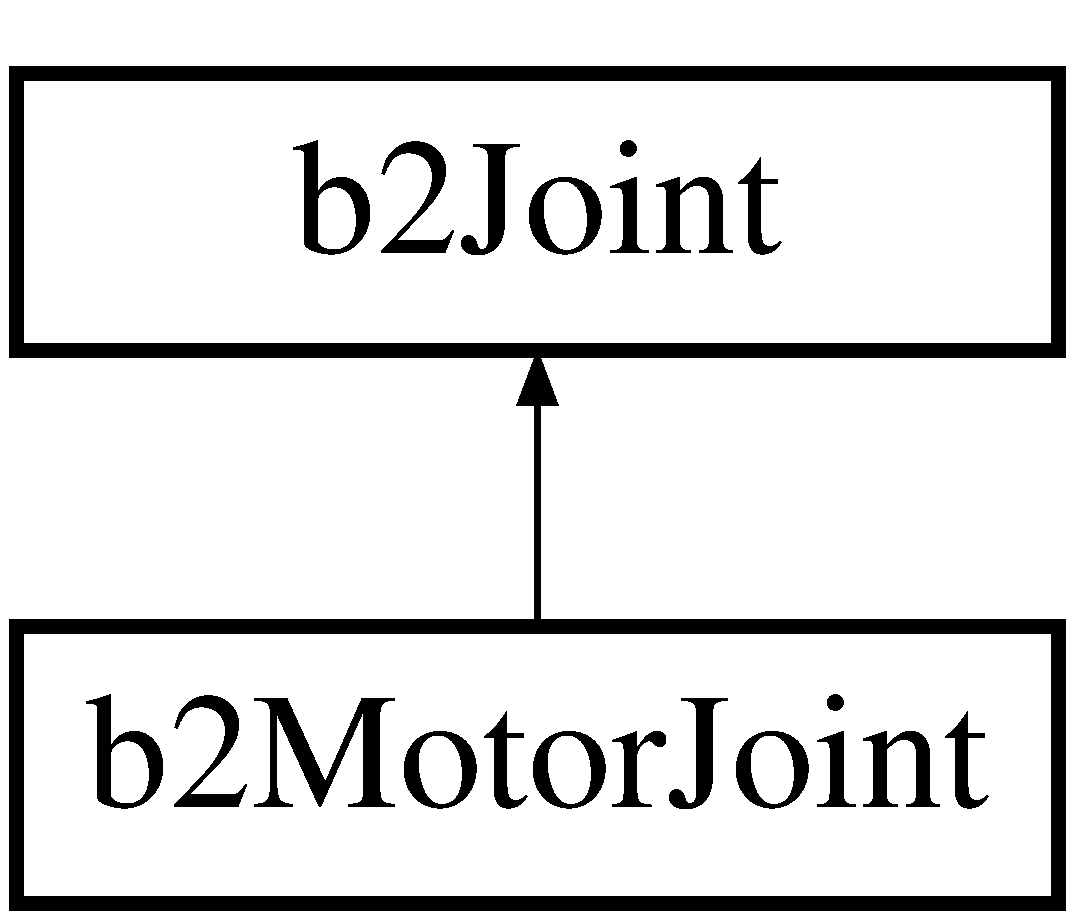
\includegraphics[height=2.000000cm]{classb2MotorJoint}
\end{center}
\end{figure}
\subsection*{Public Member Functions}
\begin{DoxyCompactItemize}
\item 
\mbox{\Hypertarget{classb2MotorJoint_a58adfab0fe79d254347a367341b0963a}\label{classb2MotorJoint_a58adfab0fe79d254347a367341b0963a}} 
\mbox{\hyperlink{structb2Vec2}{b2\+Vec2}} \mbox{\hyperlink{classb2MotorJoint_a58adfab0fe79d254347a367341b0963a}{Get\+AnchorA}} () const override
\begin{DoxyCompactList}\small\item\em Get the anchor point on bodyA in world coordinates. \end{DoxyCompactList}\item 
\mbox{\Hypertarget{classb2MotorJoint_a5d563fd070f7b6cfe8db6f83e1bebbcd}\label{classb2MotorJoint_a5d563fd070f7b6cfe8db6f83e1bebbcd}} 
\mbox{\hyperlink{structb2Vec2}{b2\+Vec2}} \mbox{\hyperlink{classb2MotorJoint_a5d563fd070f7b6cfe8db6f83e1bebbcd}{Get\+AnchorB}} () const override
\begin{DoxyCompactList}\small\item\em Get the anchor point on bodyB in world coordinates. \end{DoxyCompactList}\item 
\mbox{\Hypertarget{classb2MotorJoint_a85a3ac568e797d0620dcf4f7532ed949}\label{classb2MotorJoint_a85a3ac568e797d0620dcf4f7532ed949}} 
\mbox{\hyperlink{structb2Vec2}{b2\+Vec2}} \mbox{\hyperlink{classb2MotorJoint_a85a3ac568e797d0620dcf4f7532ed949}{Get\+Reaction\+Force}} (float32 inv\+\_\+dt) const override
\begin{DoxyCompactList}\small\item\em Get the reaction force on bodyB at the joint anchor in Newtons. \end{DoxyCompactList}\item 
\mbox{\Hypertarget{classb2MotorJoint_a542b68309e0294f8bda152eff92086d9}\label{classb2MotorJoint_a542b68309e0294f8bda152eff92086d9}} 
float32 \mbox{\hyperlink{classb2MotorJoint_a542b68309e0294f8bda152eff92086d9}{Get\+Reaction\+Torque}} (float32 inv\+\_\+dt) const override
\begin{DoxyCompactList}\small\item\em Get the reaction torque on bodyB in N$\ast$m. \end{DoxyCompactList}\item 
\mbox{\Hypertarget{classb2MotorJoint_a99254b5fc9ed9f2d0fdccada513000c3}\label{classb2MotorJoint_a99254b5fc9ed9f2d0fdccada513000c3}} 
void \mbox{\hyperlink{classb2MotorJoint_a99254b5fc9ed9f2d0fdccada513000c3}{Set\+Linear\+Offset}} (const \mbox{\hyperlink{structb2Vec2}{b2\+Vec2}} \&linear\+Offset)
\begin{DoxyCompactList}\small\item\em Set/get the target linear offset, in frame A, in meters. \end{DoxyCompactList}\item 
\mbox{\Hypertarget{classb2MotorJoint_a87a61f162e202e2f3c12200e42e3b180}\label{classb2MotorJoint_a87a61f162e202e2f3c12200e42e3b180}} 
const \mbox{\hyperlink{structb2Vec2}{b2\+Vec2}} \& {\bfseries Get\+Linear\+Offset} () const
\item 
\mbox{\Hypertarget{classb2MotorJoint_a14d7dca1767548ddffe293e39cafc3c7}\label{classb2MotorJoint_a14d7dca1767548ddffe293e39cafc3c7}} 
void \mbox{\hyperlink{classb2MotorJoint_a14d7dca1767548ddffe293e39cafc3c7}{Set\+Angular\+Offset}} (float32 angular\+Offset)
\begin{DoxyCompactList}\small\item\em Set/get the target angular offset, in radians. \end{DoxyCompactList}\item 
\mbox{\Hypertarget{classb2MotorJoint_a4dc4e5ee4ec8615c3d712ea6cac48436}\label{classb2MotorJoint_a4dc4e5ee4ec8615c3d712ea6cac48436}} 
float32 {\bfseries Get\+Angular\+Offset} () const
\item 
\mbox{\Hypertarget{classb2MotorJoint_a62f95f23d60123cebe14f2fcec155801}\label{classb2MotorJoint_a62f95f23d60123cebe14f2fcec155801}} 
void \mbox{\hyperlink{classb2MotorJoint_a62f95f23d60123cebe14f2fcec155801}{Set\+Max\+Force}} (float32 force)
\begin{DoxyCompactList}\small\item\em Set the maximum friction force in N. \end{DoxyCompactList}\item 
\mbox{\Hypertarget{classb2MotorJoint_ac7353eace38d2593a523149abe8ec2b5}\label{classb2MotorJoint_ac7353eace38d2593a523149abe8ec2b5}} 
float32 \mbox{\hyperlink{classb2MotorJoint_ac7353eace38d2593a523149abe8ec2b5}{Get\+Max\+Force}} () const
\begin{DoxyCompactList}\small\item\em Get the maximum friction force in N. \end{DoxyCompactList}\item 
\mbox{\Hypertarget{classb2MotorJoint_a3e9a259d36c36e0dc078282e6799d625}\label{classb2MotorJoint_a3e9a259d36c36e0dc078282e6799d625}} 
void \mbox{\hyperlink{classb2MotorJoint_a3e9a259d36c36e0dc078282e6799d625}{Set\+Max\+Torque}} (float32 torque)
\begin{DoxyCompactList}\small\item\em Set the maximum friction torque in N$\ast$m. \end{DoxyCompactList}\item 
\mbox{\Hypertarget{classb2MotorJoint_a40d4e4e852a6a722708f0c47b5c9fd69}\label{classb2MotorJoint_a40d4e4e852a6a722708f0c47b5c9fd69}} 
float32 \mbox{\hyperlink{classb2MotorJoint_a40d4e4e852a6a722708f0c47b5c9fd69}{Get\+Max\+Torque}} () const
\begin{DoxyCompactList}\small\item\em Get the maximum friction torque in N$\ast$m. \end{DoxyCompactList}\item 
\mbox{\Hypertarget{classb2MotorJoint_ae59e624b8a7b6f869ab5e6148352cb52}\label{classb2MotorJoint_ae59e624b8a7b6f869ab5e6148352cb52}} 
void \mbox{\hyperlink{classb2MotorJoint_ae59e624b8a7b6f869ab5e6148352cb52}{Set\+Correction\+Factor}} (float32 factor)
\begin{DoxyCompactList}\small\item\em Set the position correction factor in the range \mbox{[}0,1\mbox{]}. \end{DoxyCompactList}\item 
\mbox{\Hypertarget{classb2MotorJoint_a429f9656d9f39e6e992de59c9620d6c6}\label{classb2MotorJoint_a429f9656d9f39e6e992de59c9620d6c6}} 
float32 \mbox{\hyperlink{classb2MotorJoint_a429f9656d9f39e6e992de59c9620d6c6}{Get\+Correction\+Factor}} () const
\begin{DoxyCompactList}\small\item\em Get the position correction factor in the range \mbox{[}0,1\mbox{]}. \end{DoxyCompactList}\item 
\mbox{\Hypertarget{classb2MotorJoint_abb67754f39b4747ae07af5cb5b348836}\label{classb2MotorJoint_abb67754f39b4747ae07af5cb5b348836}} 
void \mbox{\hyperlink{classb2MotorJoint_abb67754f39b4747ae07af5cb5b348836}{Dump}} () override
\begin{DoxyCompactList}\small\item\em Dump to b2\+Log. \end{DoxyCompactList}\end{DoxyCompactItemize}
\subsection*{Protected Member Functions}
\begin{DoxyCompactItemize}
\item 
\mbox{\Hypertarget{classb2MotorJoint_ac0c56b069910915e1ceef3b89c035833}\label{classb2MotorJoint_ac0c56b069910915e1ceef3b89c035833}} 
{\bfseries b2\+Motor\+Joint} (const \mbox{\hyperlink{structb2MotorJointDef}{b2\+Motor\+Joint\+Def}} $\ast$def)
\item 
\mbox{\Hypertarget{classb2MotorJoint_aeffac9d1e3940c362962319d1bdb3f22}\label{classb2MotorJoint_aeffac9d1e3940c362962319d1bdb3f22}} 
void {\bfseries Init\+Velocity\+Constraints} (const \mbox{\hyperlink{structb2SolverData}{b2\+Solver\+Data}} \&data) override
\item 
\mbox{\Hypertarget{classb2MotorJoint_a620c75b301aeab409f9d50a041a80fb8}\label{classb2MotorJoint_a620c75b301aeab409f9d50a041a80fb8}} 
void {\bfseries Solve\+Velocity\+Constraints} (const \mbox{\hyperlink{structb2SolverData}{b2\+Solver\+Data}} \&data) override
\item 
\mbox{\Hypertarget{classb2MotorJoint_a4e56455ab7e90f82fc1f463efc9b59de}\label{classb2MotorJoint_a4e56455ab7e90f82fc1f463efc9b59de}} 
bool {\bfseries Solve\+Position\+Constraints} (const \mbox{\hyperlink{structb2SolverData}{b2\+Solver\+Data}} \&data) override
\end{DoxyCompactItemize}
\subsection*{Protected Attributes}
\begin{DoxyCompactItemize}
\item 
\mbox{\Hypertarget{classb2MotorJoint_a6e8db2001da3a9b2926a41451f28f73b}\label{classb2MotorJoint_a6e8db2001da3a9b2926a41451f28f73b}} 
\mbox{\hyperlink{structb2Vec2}{b2\+Vec2}} {\bfseries m\+\_\+linear\+Offset}
\item 
\mbox{\Hypertarget{classb2MotorJoint_ac48f242920da2d2678dea09941c3d31c}\label{classb2MotorJoint_ac48f242920da2d2678dea09941c3d31c}} 
float32 {\bfseries m\+\_\+angular\+Offset}
\item 
\mbox{\Hypertarget{classb2MotorJoint_a5aba4dbf8cccc33a1cc20f7a503b51f5}\label{classb2MotorJoint_a5aba4dbf8cccc33a1cc20f7a503b51f5}} 
\mbox{\hyperlink{structb2Vec2}{b2\+Vec2}} {\bfseries m\+\_\+linear\+Impulse}
\item 
\mbox{\Hypertarget{classb2MotorJoint_abf23ffd98f99bdf34423bee99e40a949}\label{classb2MotorJoint_abf23ffd98f99bdf34423bee99e40a949}} 
float32 {\bfseries m\+\_\+angular\+Impulse}
\item 
\mbox{\Hypertarget{classb2MotorJoint_ad9a39349f3b43e8f1c33f5a44575dffe}\label{classb2MotorJoint_ad9a39349f3b43e8f1c33f5a44575dffe}} 
float32 {\bfseries m\+\_\+max\+Force}
\item 
\mbox{\Hypertarget{classb2MotorJoint_a7c0c777bb6d78f3eff9abb8819ddb14f}\label{classb2MotorJoint_a7c0c777bb6d78f3eff9abb8819ddb14f}} 
float32 {\bfseries m\+\_\+max\+Torque}
\item 
\mbox{\Hypertarget{classb2MotorJoint_a5e42eef05987dd269be1e709172b933c}\label{classb2MotorJoint_a5e42eef05987dd269be1e709172b933c}} 
float32 {\bfseries m\+\_\+correction\+Factor}
\item 
\mbox{\Hypertarget{classb2MotorJoint_afdd9d0ebe37506dd8509ed2392fa1f56}\label{classb2MotorJoint_afdd9d0ebe37506dd8509ed2392fa1f56}} 
int32 {\bfseries m\+\_\+indexA}
\item 
\mbox{\Hypertarget{classb2MotorJoint_a51525d3f5af31dcede8e641943fe86b3}\label{classb2MotorJoint_a51525d3f5af31dcede8e641943fe86b3}} 
int32 {\bfseries m\+\_\+indexB}
\item 
\mbox{\Hypertarget{classb2MotorJoint_a0340ef47abad9882a271be45df15d3ed}\label{classb2MotorJoint_a0340ef47abad9882a271be45df15d3ed}} 
\mbox{\hyperlink{structb2Vec2}{b2\+Vec2}} {\bfseries m\+\_\+rA}
\item 
\mbox{\Hypertarget{classb2MotorJoint_a85c605b404e4b087e2932fdf23b447d5}\label{classb2MotorJoint_a85c605b404e4b087e2932fdf23b447d5}} 
\mbox{\hyperlink{structb2Vec2}{b2\+Vec2}} {\bfseries m\+\_\+rB}
\item 
\mbox{\Hypertarget{classb2MotorJoint_a42f50bbd4b5821164c9777903c83a723}\label{classb2MotorJoint_a42f50bbd4b5821164c9777903c83a723}} 
\mbox{\hyperlink{structb2Vec2}{b2\+Vec2}} {\bfseries m\+\_\+local\+CenterA}
\item 
\mbox{\Hypertarget{classb2MotorJoint_a8ba1cf76d5cbc10bf6ff9b7685ebc20d}\label{classb2MotorJoint_a8ba1cf76d5cbc10bf6ff9b7685ebc20d}} 
\mbox{\hyperlink{structb2Vec2}{b2\+Vec2}} {\bfseries m\+\_\+local\+CenterB}
\item 
\mbox{\Hypertarget{classb2MotorJoint_a21d38a7fedf735aca7d36d1ec033337e}\label{classb2MotorJoint_a21d38a7fedf735aca7d36d1ec033337e}} 
\mbox{\hyperlink{structb2Vec2}{b2\+Vec2}} {\bfseries m\+\_\+linear\+Error}
\item 
\mbox{\Hypertarget{classb2MotorJoint_a76fd4aa158014c7fd653ca47c0e3c50a}\label{classb2MotorJoint_a76fd4aa158014c7fd653ca47c0e3c50a}} 
float32 {\bfseries m\+\_\+angular\+Error}
\item 
\mbox{\Hypertarget{classb2MotorJoint_a24154e990c9c6cda65989b2828d27c1a}\label{classb2MotorJoint_a24154e990c9c6cda65989b2828d27c1a}} 
float32 {\bfseries m\+\_\+inv\+MassA}
\item 
\mbox{\Hypertarget{classb2MotorJoint_a85aff034d88bd4dcf6ab0aea28df84cb}\label{classb2MotorJoint_a85aff034d88bd4dcf6ab0aea28df84cb}} 
float32 {\bfseries m\+\_\+inv\+MassB}
\item 
\mbox{\Hypertarget{classb2MotorJoint_a873dc8487f43a0d9ec890e3f023efe26}\label{classb2MotorJoint_a873dc8487f43a0d9ec890e3f023efe26}} 
float32 {\bfseries m\+\_\+inv\+IA}
\item 
\mbox{\Hypertarget{classb2MotorJoint_a2d67befa1f4404c03cacb918f4679a48}\label{classb2MotorJoint_a2d67befa1f4404c03cacb918f4679a48}} 
float32 {\bfseries m\+\_\+inv\+IB}
\item 
\mbox{\Hypertarget{classb2MotorJoint_a89503b91fd38d332304092661aafd2c0}\label{classb2MotorJoint_a89503b91fd38d332304092661aafd2c0}} 
\mbox{\hyperlink{structb2Mat22}{b2\+Mat22}} {\bfseries m\+\_\+linear\+Mass}
\item 
\mbox{\Hypertarget{classb2MotorJoint_a3718dc3784fb4f09ecf42d28c9896ecc}\label{classb2MotorJoint_a3718dc3784fb4f09ecf42d28c9896ecc}} 
float32 {\bfseries m\+\_\+angular\+Mass}
\end{DoxyCompactItemize}
\subsection*{Friends}
\begin{DoxyCompactItemize}
\item 
\mbox{\Hypertarget{classb2MotorJoint_a54ade8ed3d794298108d7f4c4e4793fa}\label{classb2MotorJoint_a54ade8ed3d794298108d7f4c4e4793fa}} 
class {\bfseries b2\+Joint}
\end{DoxyCompactItemize}
\subsection*{Additional Inherited Members}


\subsection{Detailed Description}
A motor joint is used to control the relative motion between two bodies. A typical usage is to control the movement of a dynamic body with respect to the ground. 

The documentation for this class was generated from the following files\+:\begin{DoxyCompactItemize}
\item 
Dynamics/\+Joints/b2\+Motor\+Joint.\+h\item 
Dynamics/\+Joints/b2\+Motor\+Joint.\+cpp\end{DoxyCompactItemize}

\hypertarget{structb2MotorJointDef}{}\section{b2\+Motor\+Joint\+Def Struct Reference}
\label{structb2MotorJointDef}\index{b2\+Motor\+Joint\+Def@{b2\+Motor\+Joint\+Def}}


Motor joint definition.  




{\ttfamily \#include $<$b2\+Motor\+Joint.\+h$>$}

Inheritance diagram for b2\+Motor\+Joint\+Def\+:\begin{figure}[H]
\begin{center}
\leavevmode
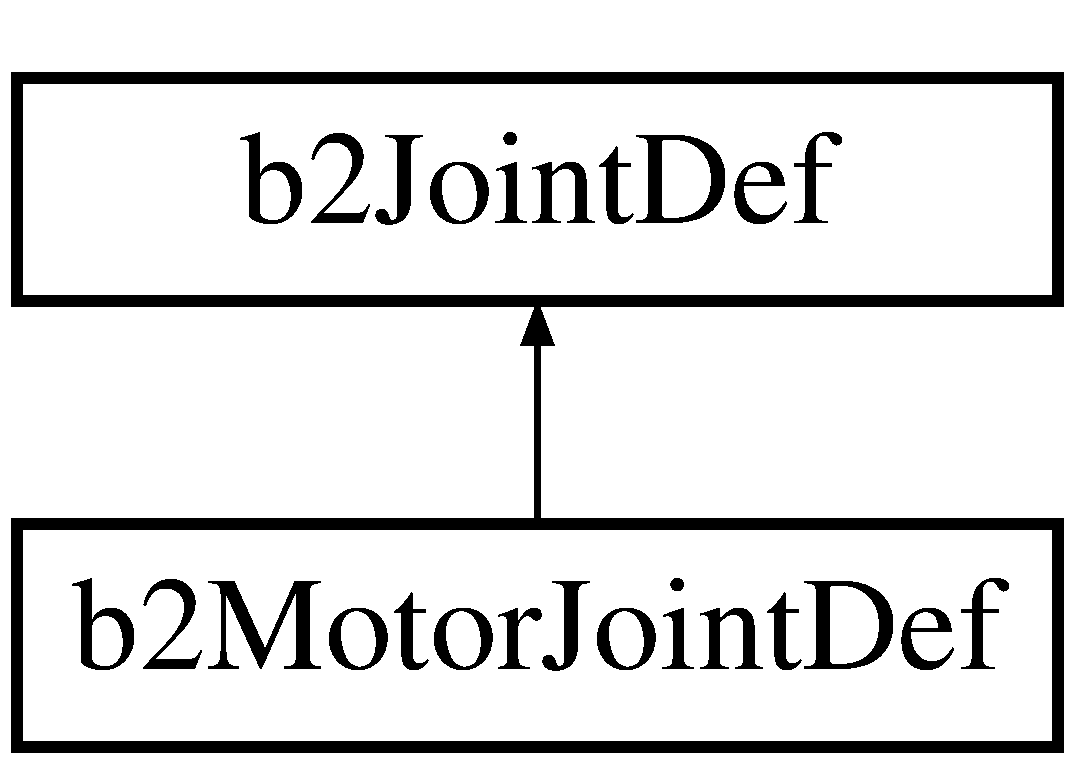
\includegraphics[height=2.000000cm]{structb2MotorJointDef}
\end{center}
\end{figure}
\subsection*{Public Member Functions}
\begin{DoxyCompactItemize}
\item 
\mbox{\Hypertarget{structb2MotorJointDef_a90eb924b6e04da8d75d9cefad0655960}\label{structb2MotorJointDef_a90eb924b6e04da8d75d9cefad0655960}} 
void \mbox{\hyperlink{structb2MotorJointDef_a90eb924b6e04da8d75d9cefad0655960}{Initialize}} (\mbox{\hyperlink{classb2Body}{b2\+Body}} $\ast$\mbox{\hyperlink{structb2JointDef_a8cd54c93da396be75a9788f2c6897f05}{bodyA}}, \mbox{\hyperlink{classb2Body}{b2\+Body}} $\ast$\mbox{\hyperlink{structb2JointDef_aa4f4dee2fbcd12187b19506b60e68e3d}{bodyB}})
\begin{DoxyCompactList}\small\item\em Initialize the bodies and offsets using the current transforms. \end{DoxyCompactList}\end{DoxyCompactItemize}
\subsection*{Public Attributes}
\begin{DoxyCompactItemize}
\item 
\mbox{\Hypertarget{structb2MotorJointDef_a2c957cffc2af66c6c8077c069b906bc4}\label{structb2MotorJointDef_a2c957cffc2af66c6c8077c069b906bc4}} 
\mbox{\hyperlink{structb2Vec2}{b2\+Vec2}} \mbox{\hyperlink{structb2MotorJointDef_a2c957cffc2af66c6c8077c069b906bc4}{linear\+Offset}}
\begin{DoxyCompactList}\small\item\em Position of bodyB minus the position of bodyA, in bodyA\textquotesingle{}s frame, in meters. \end{DoxyCompactList}\item 
\mbox{\Hypertarget{structb2MotorJointDef_abdb42eff4aeff1d48038e084c57e1cb0}\label{structb2MotorJointDef_abdb42eff4aeff1d48038e084c57e1cb0}} 
float32 \mbox{\hyperlink{structb2MotorJointDef_abdb42eff4aeff1d48038e084c57e1cb0}{angular\+Offset}}
\begin{DoxyCompactList}\small\item\em The bodyB angle minus bodyA angle in radians. \end{DoxyCompactList}\item 
\mbox{\Hypertarget{structb2MotorJointDef_a2f66d1b99c654e112dc68e15375d5ee7}\label{structb2MotorJointDef_a2f66d1b99c654e112dc68e15375d5ee7}} 
float32 \mbox{\hyperlink{structb2MotorJointDef_a2f66d1b99c654e112dc68e15375d5ee7}{max\+Force}}
\begin{DoxyCompactList}\small\item\em The maximum motor force in N. \end{DoxyCompactList}\item 
\mbox{\Hypertarget{structb2MotorJointDef_afcf5dd58166917a4574d1f28f6bb3660}\label{structb2MotorJointDef_afcf5dd58166917a4574d1f28f6bb3660}} 
float32 \mbox{\hyperlink{structb2MotorJointDef_afcf5dd58166917a4574d1f28f6bb3660}{max\+Torque}}
\begin{DoxyCompactList}\small\item\em The maximum motor torque in N-\/m. \end{DoxyCompactList}\item 
\mbox{\Hypertarget{structb2MotorJointDef_ab282afdb92d07ead23530f57fd0eb9ea}\label{structb2MotorJointDef_ab282afdb92d07ead23530f57fd0eb9ea}} 
float32 \mbox{\hyperlink{structb2MotorJointDef_ab282afdb92d07ead23530f57fd0eb9ea}{correction\+Factor}}
\begin{DoxyCompactList}\small\item\em Position correction factor in the range \mbox{[}0,1\mbox{]}. \end{DoxyCompactList}\end{DoxyCompactItemize}


\subsection{Detailed Description}
Motor joint definition. 

The documentation for this struct was generated from the following files\+:\begin{DoxyCompactItemize}
\item 
Dynamics/\+Joints/b2\+Motor\+Joint.\+h\item 
Dynamics/\+Joints/b2\+Motor\+Joint.\+cpp\end{DoxyCompactItemize}

\hypertarget{classb2MouseJoint}{}\section{b2\+Mouse\+Joint Class Reference}
\label{classb2MouseJoint}\index{b2\+Mouse\+Joint@{b2\+Mouse\+Joint}}


{\ttfamily \#include $<$b2\+Mouse\+Joint.\+h$>$}

Inheritance diagram for b2\+Mouse\+Joint\+:\begin{figure}[H]
\begin{center}
\leavevmode
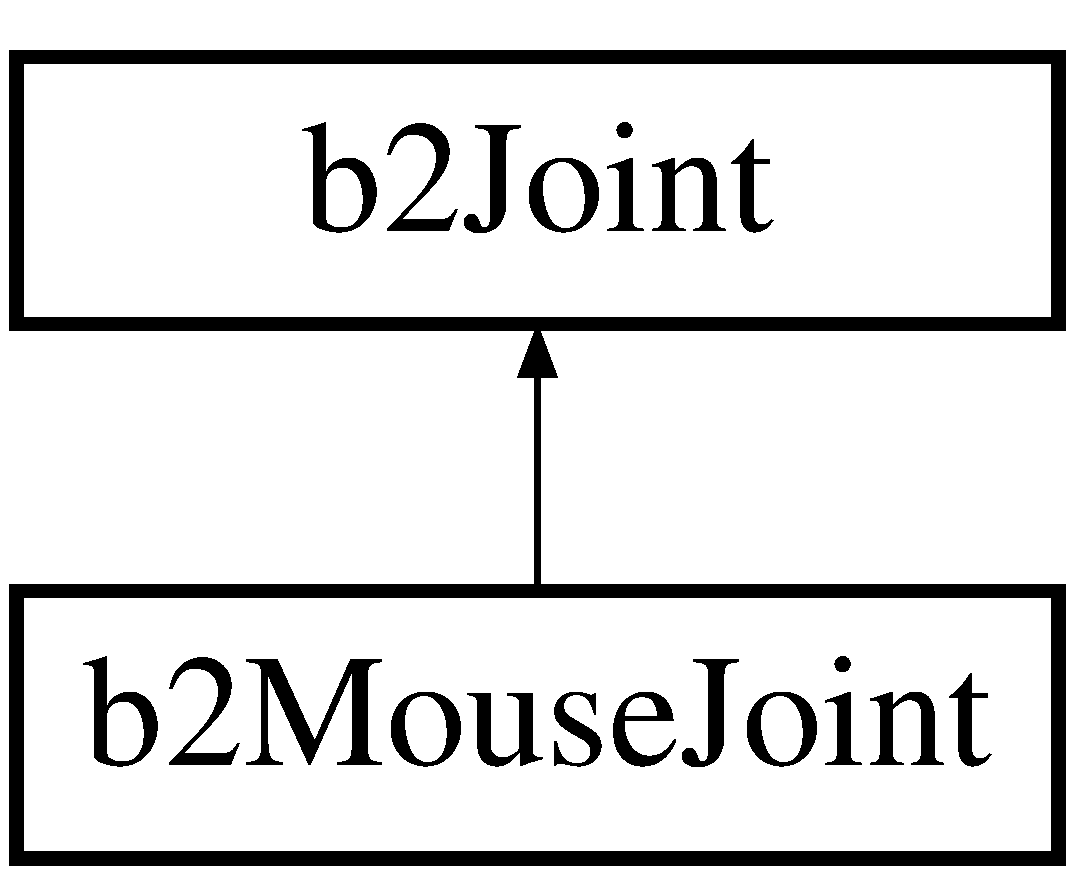
\includegraphics[height=2.000000cm]{classb2MouseJoint}
\end{center}
\end{figure}
\subsection*{Public Member Functions}
\begin{DoxyCompactItemize}
\item 
\mbox{\Hypertarget{classb2MouseJoint_a3c42531ac763bca3658a987d0ac7d2c4}\label{classb2MouseJoint_a3c42531ac763bca3658a987d0ac7d2c4}} 
\mbox{\hyperlink{structb2Vec2}{b2\+Vec2}} \mbox{\hyperlink{classb2MouseJoint_a3c42531ac763bca3658a987d0ac7d2c4}{Get\+AnchorA}} () const override
\begin{DoxyCompactList}\small\item\em Implements \mbox{\hyperlink{classb2Joint}{b2\+Joint}}. \end{DoxyCompactList}\item 
\mbox{\Hypertarget{classb2MouseJoint_adecfaff123ba199f9fc80be7fcb74af2}\label{classb2MouseJoint_adecfaff123ba199f9fc80be7fcb74af2}} 
\mbox{\hyperlink{structb2Vec2}{b2\+Vec2}} \mbox{\hyperlink{classb2MouseJoint_adecfaff123ba199f9fc80be7fcb74af2}{Get\+AnchorB}} () const override
\begin{DoxyCompactList}\small\item\em Implements \mbox{\hyperlink{classb2Joint}{b2\+Joint}}. \end{DoxyCompactList}\item 
\mbox{\Hypertarget{classb2MouseJoint_a1af7bb9f41076b29a1ddefd7b6c2f27b}\label{classb2MouseJoint_a1af7bb9f41076b29a1ddefd7b6c2f27b}} 
\mbox{\hyperlink{structb2Vec2}{b2\+Vec2}} \mbox{\hyperlink{classb2MouseJoint_a1af7bb9f41076b29a1ddefd7b6c2f27b}{Get\+Reaction\+Force}} (float32 inv\+\_\+dt) const override
\begin{DoxyCompactList}\small\item\em Implements \mbox{\hyperlink{classb2Joint}{b2\+Joint}}. \end{DoxyCompactList}\item 
\mbox{\Hypertarget{classb2MouseJoint_aa9ea0d1b1aa2db5be3ed63392a7e28a2}\label{classb2MouseJoint_aa9ea0d1b1aa2db5be3ed63392a7e28a2}} 
float32 \mbox{\hyperlink{classb2MouseJoint_aa9ea0d1b1aa2db5be3ed63392a7e28a2}{Get\+Reaction\+Torque}} (float32 inv\+\_\+dt) const override
\begin{DoxyCompactList}\small\item\em Implements \mbox{\hyperlink{classb2Joint}{b2\+Joint}}. \end{DoxyCompactList}\item 
\mbox{\Hypertarget{classb2MouseJoint_a96f34c1c990407eddbadf07ae359b1f3}\label{classb2MouseJoint_a96f34c1c990407eddbadf07ae359b1f3}} 
void \mbox{\hyperlink{classb2MouseJoint_a96f34c1c990407eddbadf07ae359b1f3}{Set\+Target}} (const \mbox{\hyperlink{structb2Vec2}{b2\+Vec2}} \&target)
\begin{DoxyCompactList}\small\item\em Use this to update the target point. \end{DoxyCompactList}\item 
\mbox{\Hypertarget{classb2MouseJoint_a9904bbdf5b73f49954f37c27c983d715}\label{classb2MouseJoint_a9904bbdf5b73f49954f37c27c983d715}} 
const \mbox{\hyperlink{structb2Vec2}{b2\+Vec2}} \& {\bfseries Get\+Target} () const
\item 
\mbox{\Hypertarget{classb2MouseJoint_a4beba6ea0827960fac2474563591c03a}\label{classb2MouseJoint_a4beba6ea0827960fac2474563591c03a}} 
void \mbox{\hyperlink{classb2MouseJoint_a4beba6ea0827960fac2474563591c03a}{Set\+Max\+Force}} (float32 force)
\begin{DoxyCompactList}\small\item\em Set/get the maximum force in Newtons. \end{DoxyCompactList}\item 
\mbox{\Hypertarget{classb2MouseJoint_a61c9fbd78498d3484f824876654eb015}\label{classb2MouseJoint_a61c9fbd78498d3484f824876654eb015}} 
float32 {\bfseries Get\+Max\+Force} () const
\item 
\mbox{\Hypertarget{classb2MouseJoint_a8b37706535923637ca280c5a0467b14d}\label{classb2MouseJoint_a8b37706535923637ca280c5a0467b14d}} 
void \mbox{\hyperlink{classb2MouseJoint_a8b37706535923637ca280c5a0467b14d}{Set\+Frequency}} (float32 hz)
\begin{DoxyCompactList}\small\item\em Set/get the frequency in Hertz. \end{DoxyCompactList}\item 
\mbox{\Hypertarget{classb2MouseJoint_a97b9264cc357ac96e447990f52086719}\label{classb2MouseJoint_a97b9264cc357ac96e447990f52086719}} 
float32 {\bfseries Get\+Frequency} () const
\item 
\mbox{\Hypertarget{classb2MouseJoint_a648c8f3ecb82f4887c0eefcfe48cbd37}\label{classb2MouseJoint_a648c8f3ecb82f4887c0eefcfe48cbd37}} 
void \mbox{\hyperlink{classb2MouseJoint_a648c8f3ecb82f4887c0eefcfe48cbd37}{Set\+Damping\+Ratio}} (float32 ratio)
\begin{DoxyCompactList}\small\item\em Set/get the damping ratio (dimensionless). \end{DoxyCompactList}\item 
\mbox{\Hypertarget{classb2MouseJoint_a551de1d56a743e71684a1382054c17c9}\label{classb2MouseJoint_a551de1d56a743e71684a1382054c17c9}} 
float32 {\bfseries Get\+Damping\+Ratio} () const
\item 
\mbox{\Hypertarget{classb2MouseJoint_aea1ff1e5b71ba5630875585cab1e2a96}\label{classb2MouseJoint_aea1ff1e5b71ba5630875585cab1e2a96}} 
void \mbox{\hyperlink{classb2MouseJoint_aea1ff1e5b71ba5630875585cab1e2a96}{Dump}} () override
\begin{DoxyCompactList}\small\item\em The mouse joint does not support dumping. \end{DoxyCompactList}\item 
\mbox{\Hypertarget{classb2MouseJoint_a9b1b2671837495be175e496afb622904}\label{classb2MouseJoint_a9b1b2671837495be175e496afb622904}} 
void \mbox{\hyperlink{classb2MouseJoint_a9b1b2671837495be175e496afb622904}{Shift\+Origin}} (const \mbox{\hyperlink{structb2Vec2}{b2\+Vec2}} \&new\+Origin) override
\begin{DoxyCompactList}\small\item\em Implement \mbox{\hyperlink{classb2Joint_a7804f649e993dc0fd9ae47fde5601f90}{b2\+Joint\+::\+Shift\+Origin}}. \end{DoxyCompactList}\end{DoxyCompactItemize}
\subsection*{Protected Member Functions}
\begin{DoxyCompactItemize}
\item 
\mbox{\Hypertarget{classb2MouseJoint_ad147d7989d884952c3389f7e5e3acf68}\label{classb2MouseJoint_ad147d7989d884952c3389f7e5e3acf68}} 
{\bfseries b2\+Mouse\+Joint} (const \mbox{\hyperlink{structb2MouseJointDef}{b2\+Mouse\+Joint\+Def}} $\ast$def)
\item 
\mbox{\Hypertarget{classb2MouseJoint_a02c342a98cfa5687de2bd3dba7c700b1}\label{classb2MouseJoint_a02c342a98cfa5687de2bd3dba7c700b1}} 
void {\bfseries Init\+Velocity\+Constraints} (const \mbox{\hyperlink{structb2SolverData}{b2\+Solver\+Data}} \&data) override
\item 
\mbox{\Hypertarget{classb2MouseJoint_a9256297320a1a67e9dc49b70f4798dd8}\label{classb2MouseJoint_a9256297320a1a67e9dc49b70f4798dd8}} 
void {\bfseries Solve\+Velocity\+Constraints} (const \mbox{\hyperlink{structb2SolverData}{b2\+Solver\+Data}} \&data) override
\item 
\mbox{\Hypertarget{classb2MouseJoint_a13f9ec996eff59c15e6330a8c3f5ba9f}\label{classb2MouseJoint_a13f9ec996eff59c15e6330a8c3f5ba9f}} 
bool {\bfseries Solve\+Position\+Constraints} (const \mbox{\hyperlink{structb2SolverData}{b2\+Solver\+Data}} \&data) override
\end{DoxyCompactItemize}
\subsection*{Protected Attributes}
\begin{DoxyCompactItemize}
\item 
\mbox{\Hypertarget{classb2MouseJoint_a11564027dbf4ecbe593d6b8c3b634ea8}\label{classb2MouseJoint_a11564027dbf4ecbe593d6b8c3b634ea8}} 
\mbox{\hyperlink{structb2Vec2}{b2\+Vec2}} {\bfseries m\+\_\+local\+AnchorB}
\item 
\mbox{\Hypertarget{classb2MouseJoint_a4196e32b3b8dfca298e37b7787245c6f}\label{classb2MouseJoint_a4196e32b3b8dfca298e37b7787245c6f}} 
\mbox{\hyperlink{structb2Vec2}{b2\+Vec2}} {\bfseries m\+\_\+targetA}
\item 
\mbox{\Hypertarget{classb2MouseJoint_a17a95ce26e366e288ca19e65abf6fd6b}\label{classb2MouseJoint_a17a95ce26e366e288ca19e65abf6fd6b}} 
float32 {\bfseries m\+\_\+frequency\+Hz}
\item 
\mbox{\Hypertarget{classb2MouseJoint_afdd1fd651a936ce0afc85decd67b7e1c}\label{classb2MouseJoint_afdd1fd651a936ce0afc85decd67b7e1c}} 
float32 {\bfseries m\+\_\+damping\+Ratio}
\item 
\mbox{\Hypertarget{classb2MouseJoint_afb358e67d625526316bc2f53a1e3cae0}\label{classb2MouseJoint_afb358e67d625526316bc2f53a1e3cae0}} 
float32 {\bfseries m\+\_\+beta}
\item 
\mbox{\Hypertarget{classb2MouseJoint_ae35319e2e64dbf3c48dd20fe8c031ebd}\label{classb2MouseJoint_ae35319e2e64dbf3c48dd20fe8c031ebd}} 
\mbox{\hyperlink{structb2Vec2}{b2\+Vec2}} {\bfseries m\+\_\+impulse}
\item 
\mbox{\Hypertarget{classb2MouseJoint_a4659e3fee0beaeac207a013095748bc1}\label{classb2MouseJoint_a4659e3fee0beaeac207a013095748bc1}} 
float32 {\bfseries m\+\_\+max\+Force}
\item 
\mbox{\Hypertarget{classb2MouseJoint_a63257ae0faad5c8ff00c92a4eaac50e0}\label{classb2MouseJoint_a63257ae0faad5c8ff00c92a4eaac50e0}} 
float32 {\bfseries m\+\_\+gamma}
\item 
\mbox{\Hypertarget{classb2MouseJoint_ae6f4a011469a55cd2c61e8338fbd4994}\label{classb2MouseJoint_ae6f4a011469a55cd2c61e8338fbd4994}} 
int32 {\bfseries m\+\_\+indexA}
\item 
\mbox{\Hypertarget{classb2MouseJoint_a5b2c7802674942419c89f140c7db85b3}\label{classb2MouseJoint_a5b2c7802674942419c89f140c7db85b3}} 
int32 {\bfseries m\+\_\+indexB}
\item 
\mbox{\Hypertarget{classb2MouseJoint_a00510096c1433e6d7e671cf5bbb1c118}\label{classb2MouseJoint_a00510096c1433e6d7e671cf5bbb1c118}} 
\mbox{\hyperlink{structb2Vec2}{b2\+Vec2}} {\bfseries m\+\_\+rB}
\item 
\mbox{\Hypertarget{classb2MouseJoint_ad9947876df55f4b4e7d435941234e22e}\label{classb2MouseJoint_ad9947876df55f4b4e7d435941234e22e}} 
\mbox{\hyperlink{structb2Vec2}{b2\+Vec2}} {\bfseries m\+\_\+local\+CenterB}
\item 
\mbox{\Hypertarget{classb2MouseJoint_a84c405322a35b0f2649071cdcd7be0fb}\label{classb2MouseJoint_a84c405322a35b0f2649071cdcd7be0fb}} 
float32 {\bfseries m\+\_\+inv\+MassB}
\item 
\mbox{\Hypertarget{classb2MouseJoint_a0a4959ae588d0071d97424e36f15228e}\label{classb2MouseJoint_a0a4959ae588d0071d97424e36f15228e}} 
float32 {\bfseries m\+\_\+inv\+IB}
\item 
\mbox{\Hypertarget{classb2MouseJoint_a628b7a7a2cd2b50313daea30baf47c4e}\label{classb2MouseJoint_a628b7a7a2cd2b50313daea30baf47c4e}} 
\mbox{\hyperlink{structb2Mat22}{b2\+Mat22}} {\bfseries m\+\_\+mass}
\item 
\mbox{\Hypertarget{classb2MouseJoint_a7ea02e17cdde70717e84bf44614275fb}\label{classb2MouseJoint_a7ea02e17cdde70717e84bf44614275fb}} 
\mbox{\hyperlink{structb2Vec2}{b2\+Vec2}} {\bfseries m\+\_\+C}
\end{DoxyCompactItemize}
\subsection*{Friends}
\begin{DoxyCompactItemize}
\item 
\mbox{\Hypertarget{classb2MouseJoint_a54ade8ed3d794298108d7f4c4e4793fa}\label{classb2MouseJoint_a54ade8ed3d794298108d7f4c4e4793fa}} 
class {\bfseries b2\+Joint}
\end{DoxyCompactItemize}
\subsection*{Additional Inherited Members}


\subsection{Detailed Description}
A mouse joint is used to make a point on a body track a specified world point. This a soft constraint with a maximum force. This allows the constraint to stretch and without applying huge forces. N\+O\+TE\+: this joint is not documented in the manual because it was developed to be used in the testbed. If you want to learn how to use the mouse joint, look at the testbed. 

The documentation for this class was generated from the following files\+:\begin{DoxyCompactItemize}
\item 
Dynamics/\+Joints/b2\+Mouse\+Joint.\+h\item 
Dynamics/\+Joints/b2\+Mouse\+Joint.\+cpp\end{DoxyCompactItemize}

\hypertarget{structb2MouseJointDef}{}\section{b2\+Mouse\+Joint\+Def Struct Reference}
\label{structb2MouseJointDef}\index{b2\+Mouse\+Joint\+Def@{b2\+Mouse\+Joint\+Def}}


{\ttfamily \#include $<$b2\+Mouse\+Joint.\+h$>$}

Inheritance diagram for b2\+Mouse\+Joint\+Def\+:\begin{figure}[H]
\begin{center}
\leavevmode
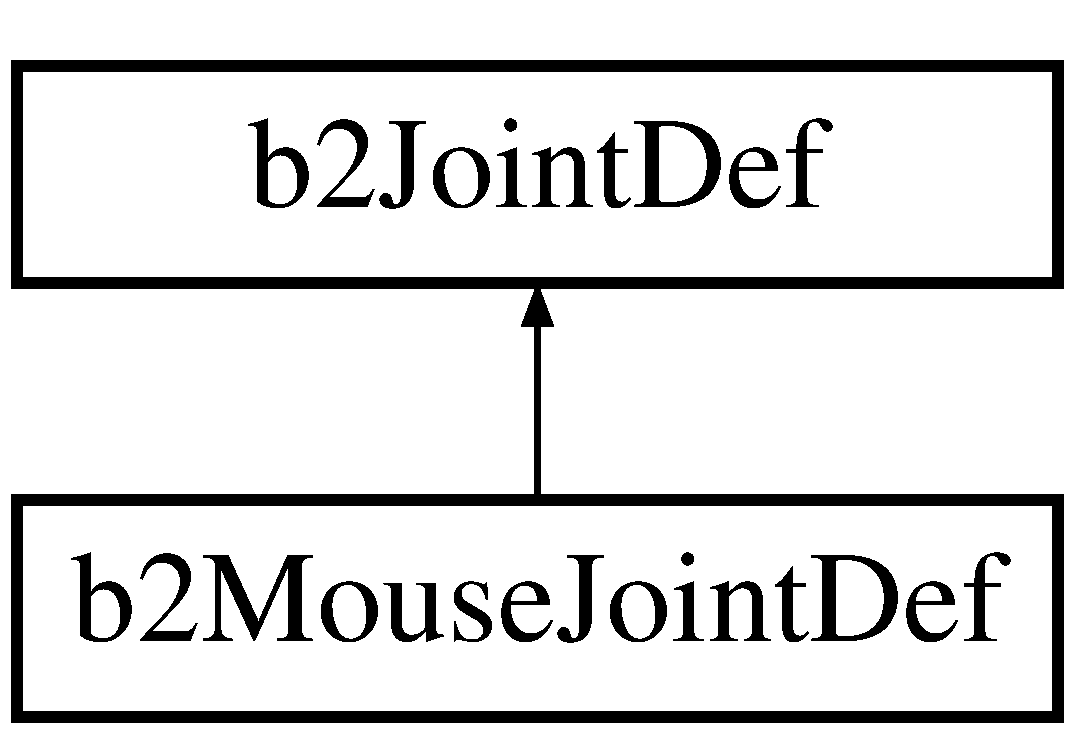
\includegraphics[height=2.000000cm]{structb2MouseJointDef}
\end{center}
\end{figure}
\subsection*{Public Attributes}
\begin{DoxyCompactItemize}
\item 
\mbox{\hyperlink{structb2Vec2}{b2\+Vec2}} \mbox{\hyperlink{structb2MouseJointDef_aa1b76f72df9aca8d42bdc3e9922e310a}{target}}
\item 
float32 \mbox{\hyperlink{structb2MouseJointDef_ae9c52b3afda8ed006eb62fad163cdc3b}{max\+Force}}
\item 
\mbox{\Hypertarget{structb2MouseJointDef_a61e9017eb928608f75edddb6e0ca7f63}\label{structb2MouseJointDef_a61e9017eb928608f75edddb6e0ca7f63}} 
float32 \mbox{\hyperlink{structb2MouseJointDef_a61e9017eb928608f75edddb6e0ca7f63}{frequency\+Hz}}
\begin{DoxyCompactList}\small\item\em The response speed. \end{DoxyCompactList}\item 
\mbox{\Hypertarget{structb2MouseJointDef_aee42888dab204a5c5745ba61acbfb7d6}\label{structb2MouseJointDef_aee42888dab204a5c5745ba61acbfb7d6}} 
float32 \mbox{\hyperlink{structb2MouseJointDef_aee42888dab204a5c5745ba61acbfb7d6}{damping\+Ratio}}
\begin{DoxyCompactList}\small\item\em The damping ratio. 0 = no damping, 1 = critical damping. \end{DoxyCompactList}\end{DoxyCompactItemize}


\subsection{Detailed Description}
Mouse joint definition. This requires a world target point, tuning parameters, and the time step. 

\subsection{Member Data Documentation}
\mbox{\Hypertarget{structb2MouseJointDef_ae9c52b3afda8ed006eb62fad163cdc3b}\label{structb2MouseJointDef_ae9c52b3afda8ed006eb62fad163cdc3b}} 
\index{b2\+Mouse\+Joint\+Def@{b2\+Mouse\+Joint\+Def}!max\+Force@{max\+Force}}
\index{max\+Force@{max\+Force}!b2\+Mouse\+Joint\+Def@{b2\+Mouse\+Joint\+Def}}
\subsubsection{\texorpdfstring{max\+Force}{maxForce}}
{\footnotesize\ttfamily float32 b2\+Mouse\+Joint\+Def\+::max\+Force}

The maximum constraint force that can be exerted to move the candidate body. Usually you will express as some multiple of the weight (multiplier $\ast$ mass $\ast$ gravity). \mbox{\Hypertarget{structb2MouseJointDef_aa1b76f72df9aca8d42bdc3e9922e310a}\label{structb2MouseJointDef_aa1b76f72df9aca8d42bdc3e9922e310a}} 
\index{b2\+Mouse\+Joint\+Def@{b2\+Mouse\+Joint\+Def}!target@{target}}
\index{target@{target}!b2\+Mouse\+Joint\+Def@{b2\+Mouse\+Joint\+Def}}
\subsubsection{\texorpdfstring{target}{target}}
{\footnotesize\ttfamily \mbox{\hyperlink{structb2Vec2}{b2\+Vec2}} b2\+Mouse\+Joint\+Def\+::target}

The initial world target point. This is assumed to coincide with the body anchor initially. 

The documentation for this struct was generated from the following file\+:\begin{DoxyCompactItemize}
\item 
Dynamics/\+Joints/b2\+Mouse\+Joint.\+h\end{DoxyCompactItemize}

\hypertarget{structb2Pair}{}\section{b2\+Pair Struct Reference}
\label{structb2Pair}\index{b2\+Pair@{b2\+Pair}}
\subsection*{Public Attributes}
\begin{DoxyCompactItemize}
\item 
\mbox{\Hypertarget{structb2Pair_abae3df5e877cf0c4611334e3eec4b84c}\label{structb2Pair_abae3df5e877cf0c4611334e3eec4b84c}} 
int32 {\bfseries proxy\+IdA}
\item 
\mbox{\Hypertarget{structb2Pair_af2bd888ccb34535ab9126497349da749}\label{structb2Pair_af2bd888ccb34535ab9126497349da749}} 
int32 {\bfseries proxy\+IdB}
\end{DoxyCompactItemize}


The documentation for this struct was generated from the following file\+:\begin{DoxyCompactItemize}
\item 
Collision/b2\+Broad\+Phase.\+h\end{DoxyCompactItemize}

\hypertarget{classb2PolygonAndCircleContact}{}\section{b2\+Polygon\+And\+Circle\+Contact Class Reference}
\label{classb2PolygonAndCircleContact}\index{b2\+Polygon\+And\+Circle\+Contact@{b2\+Polygon\+And\+Circle\+Contact}}
Inheritance diagram for b2\+Polygon\+And\+Circle\+Contact\+:\begin{figure}[H]
\begin{center}
\leavevmode
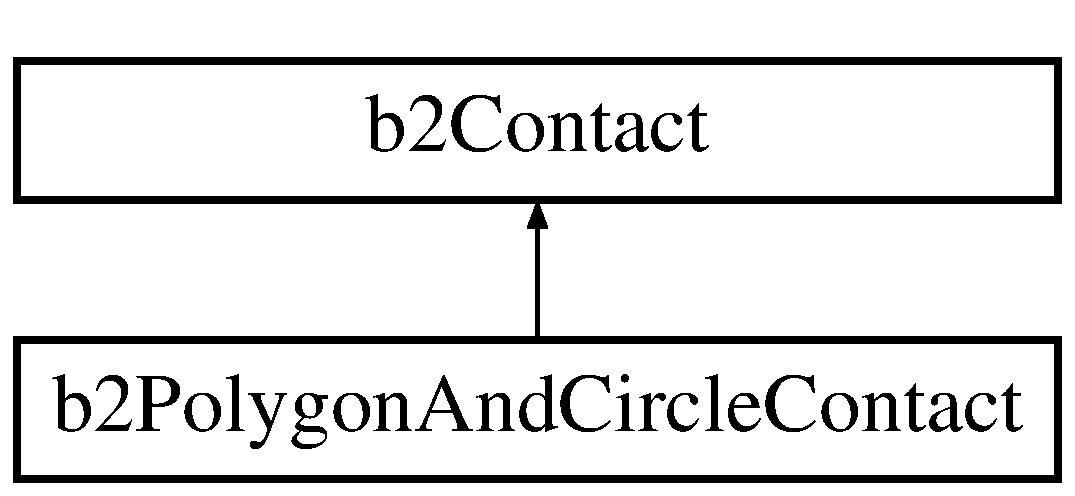
\includegraphics[height=2.000000cm]{classb2PolygonAndCircleContact}
\end{center}
\end{figure}
\subsection*{Public Member Functions}
\begin{DoxyCompactItemize}
\item 
\mbox{\Hypertarget{classb2PolygonAndCircleContact_a38158da229eee22253c1f64df1982e40}\label{classb2PolygonAndCircleContact_a38158da229eee22253c1f64df1982e40}} 
{\bfseries b2\+Polygon\+And\+Circle\+Contact} (\mbox{\hyperlink{classb2Fixture}{b2\+Fixture}} $\ast$fixtureA, \mbox{\hyperlink{classb2Fixture}{b2\+Fixture}} $\ast$fixtureB)
\item 
\mbox{\Hypertarget{classb2PolygonAndCircleContact_a4af8338f124be0b7ec704997be4736b1}\label{classb2PolygonAndCircleContact_a4af8338f124be0b7ec704997be4736b1}} 
void \mbox{\hyperlink{classb2PolygonAndCircleContact_a4af8338f124be0b7ec704997be4736b1}{Evaluate}} (\mbox{\hyperlink{structb2Manifold}{b2\+Manifold}} $\ast$manifold, const \mbox{\hyperlink{structb2Transform}{b2\+Transform}} \&xfA, const \mbox{\hyperlink{structb2Transform}{b2\+Transform}} \&xfB) override
\begin{DoxyCompactList}\small\item\em Evaluate this contact with your own manifold and transforms. \end{DoxyCompactList}\end{DoxyCompactItemize}
\subsection*{Static Public Member Functions}
\begin{DoxyCompactItemize}
\item 
\mbox{\Hypertarget{classb2PolygonAndCircleContact_a0b83e092a7d14f9cdd919fa15ef6058f}\label{classb2PolygonAndCircleContact_a0b83e092a7d14f9cdd919fa15ef6058f}} 
static \mbox{\hyperlink{classb2Contact}{b2\+Contact}} $\ast$ {\bfseries Create} (\mbox{\hyperlink{classb2Fixture}{b2\+Fixture}} $\ast$fixtureA, int32 indexA, \mbox{\hyperlink{classb2Fixture}{b2\+Fixture}} $\ast$fixtureB, int32 indexB, \mbox{\hyperlink{classb2BlockAllocator}{b2\+Block\+Allocator}} $\ast$allocator)
\item 
\mbox{\Hypertarget{classb2PolygonAndCircleContact_a04e9a3fcdcf52821fb90b8206b8bb2f0}\label{classb2PolygonAndCircleContact_a04e9a3fcdcf52821fb90b8206b8bb2f0}} 
static void {\bfseries Destroy} (\mbox{\hyperlink{classb2Contact}{b2\+Contact}} $\ast$contact, \mbox{\hyperlink{classb2BlockAllocator}{b2\+Block\+Allocator}} $\ast$allocator)
\end{DoxyCompactItemize}
\subsection*{Additional Inherited Members}


The documentation for this class was generated from the following files\+:\begin{DoxyCompactItemize}
\item 
Dynamics/\+Contacts/b2\+Polygon\+And\+Circle\+Contact.\+h\item 
Dynamics/\+Contacts/b2\+Polygon\+And\+Circle\+Contact.\+cpp\end{DoxyCompactItemize}

\hypertarget{classb2PolygonContact}{}\section{b2\+Polygon\+Contact Class Reference}
\label{classb2PolygonContact}\index{b2\+Polygon\+Contact@{b2\+Polygon\+Contact}}
Inheritance diagram for b2\+Polygon\+Contact\+:\begin{figure}[H]
\begin{center}
\leavevmode
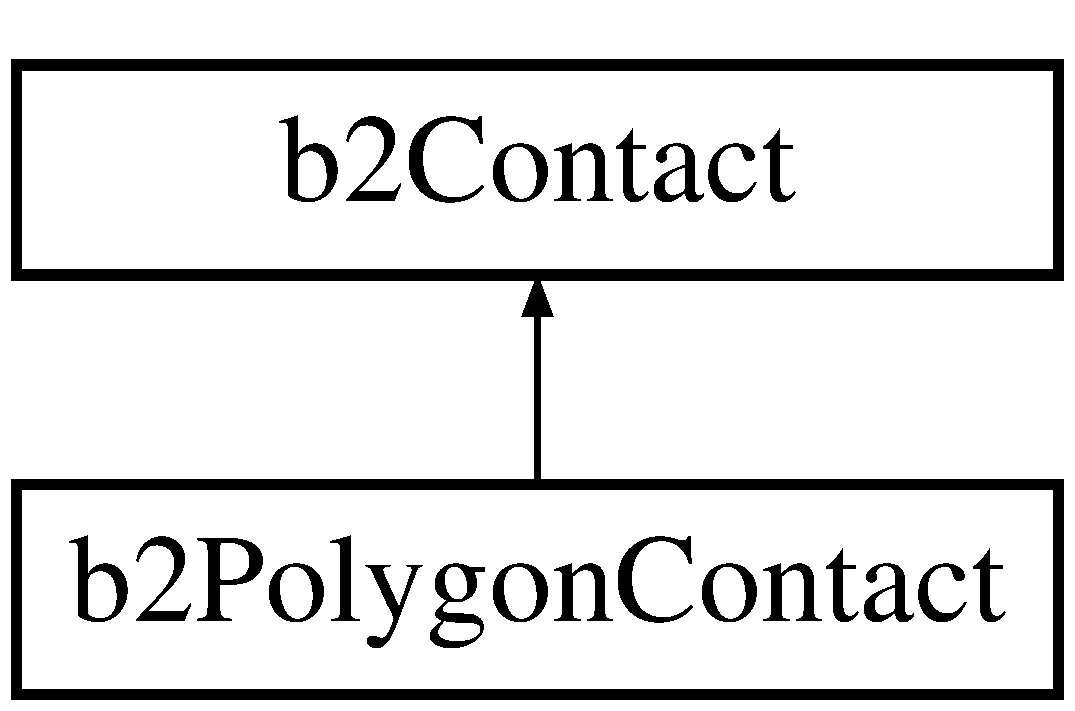
\includegraphics[height=2.000000cm]{classb2PolygonContact}
\end{center}
\end{figure}
\subsection*{Public Member Functions}
\begin{DoxyCompactItemize}
\item 
\mbox{\Hypertarget{classb2PolygonContact_a93cabf086e75ae40dcd1881760c71c63}\label{classb2PolygonContact_a93cabf086e75ae40dcd1881760c71c63}} 
{\bfseries b2\+Polygon\+Contact} (\mbox{\hyperlink{classb2Fixture}{b2\+Fixture}} $\ast$fixtureA, \mbox{\hyperlink{classb2Fixture}{b2\+Fixture}} $\ast$fixtureB)
\item 
\mbox{\Hypertarget{classb2PolygonContact_aa9581ba4a2bc769b80e3f107801d0950}\label{classb2PolygonContact_aa9581ba4a2bc769b80e3f107801d0950}} 
void \mbox{\hyperlink{classb2PolygonContact_aa9581ba4a2bc769b80e3f107801d0950}{Evaluate}} (\mbox{\hyperlink{structb2Manifold}{b2\+Manifold}} $\ast$manifold, const \mbox{\hyperlink{structb2Transform}{b2\+Transform}} \&xfA, const \mbox{\hyperlink{structb2Transform}{b2\+Transform}} \&xfB) override
\begin{DoxyCompactList}\small\item\em Evaluate this contact with your own manifold and transforms. \end{DoxyCompactList}\end{DoxyCompactItemize}
\subsection*{Static Public Member Functions}
\begin{DoxyCompactItemize}
\item 
\mbox{\Hypertarget{classb2PolygonContact_a65356af432d877838e14755c5eb3c553}\label{classb2PolygonContact_a65356af432d877838e14755c5eb3c553}} 
static \mbox{\hyperlink{classb2Contact}{b2\+Contact}} $\ast$ {\bfseries Create} (\mbox{\hyperlink{classb2Fixture}{b2\+Fixture}} $\ast$fixtureA, int32 indexA, \mbox{\hyperlink{classb2Fixture}{b2\+Fixture}} $\ast$fixtureB, int32 indexB, \mbox{\hyperlink{classb2BlockAllocator}{b2\+Block\+Allocator}} $\ast$allocator)
\item 
\mbox{\Hypertarget{classb2PolygonContact_a0cb55fd6af6f49d36c3cda15ffd96e63}\label{classb2PolygonContact_a0cb55fd6af6f49d36c3cda15ffd96e63}} 
static void {\bfseries Destroy} (\mbox{\hyperlink{classb2Contact}{b2\+Contact}} $\ast$contact, \mbox{\hyperlink{classb2BlockAllocator}{b2\+Block\+Allocator}} $\ast$allocator)
\end{DoxyCompactItemize}
\subsection*{Additional Inherited Members}


The documentation for this class was generated from the following files\+:\begin{DoxyCompactItemize}
\item 
Dynamics/\+Contacts/b2\+Polygon\+Contact.\+h\item 
Dynamics/\+Contacts/b2\+Polygon\+Contact.\+cpp\end{DoxyCompactItemize}

\hypertarget{classb2PolygonShape}{}\section{b2\+Polygon\+Shape Class Reference}
\label{classb2PolygonShape}\index{b2\+Polygon\+Shape@{b2\+Polygon\+Shape}}


{\ttfamily \#include $<$b2\+Polygon\+Shape.\+h$>$}

Inheritance diagram for b2\+Polygon\+Shape\+:\begin{figure}[H]
\begin{center}
\leavevmode
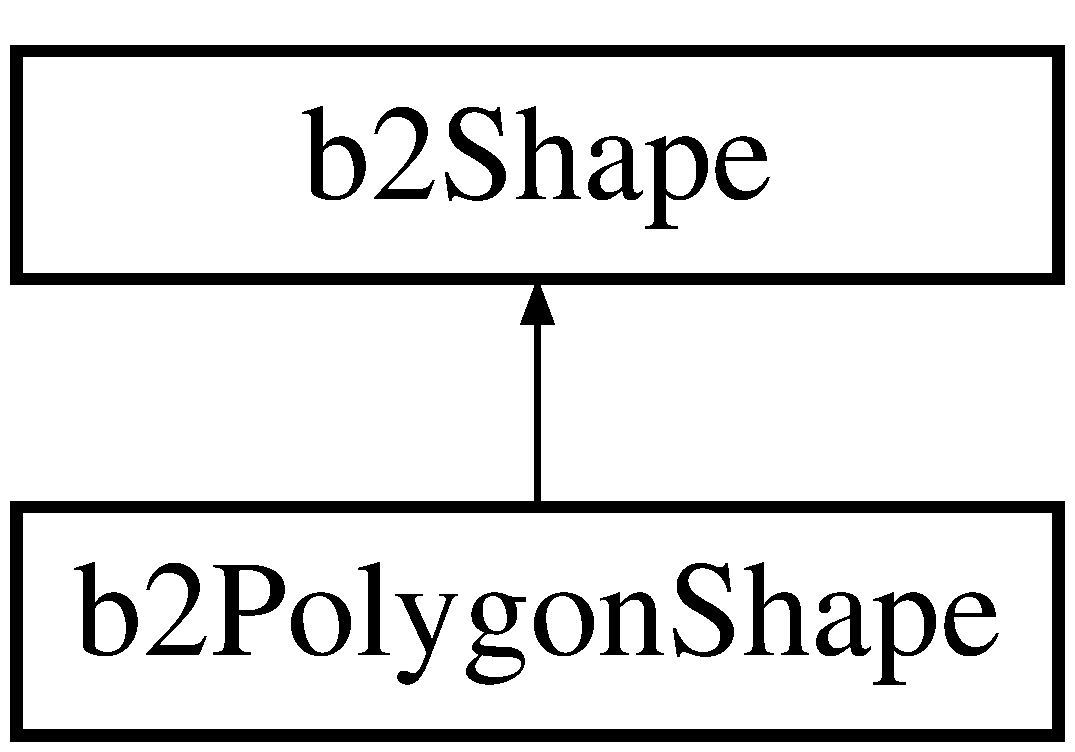
\includegraphics[height=2.000000cm]{classb2PolygonShape}
\end{center}
\end{figure}
\subsection*{Public Member Functions}
\begin{DoxyCompactItemize}
\item 
\mbox{\Hypertarget{classb2PolygonShape_ae2c2343be33db465f7e83db2061fdd51}\label{classb2PolygonShape_ae2c2343be33db465f7e83db2061fdd51}} 
\mbox{\hyperlink{classb2Shape}{b2\+Shape}} $\ast$ \mbox{\hyperlink{classb2PolygonShape_ae2c2343be33db465f7e83db2061fdd51}{Clone}} (\mbox{\hyperlink{classb2BlockAllocator}{b2\+Block\+Allocator}} $\ast$allocator) const override
\begin{DoxyCompactList}\small\item\em Implement \mbox{\hyperlink{classb2Shape}{b2\+Shape}}. \end{DoxyCompactList}\item 
int32 \mbox{\hyperlink{classb2PolygonShape_aa8bb0d5a88624104425cdee0b2f4427a}{Get\+Child\+Count}} () const override
\item 
void \mbox{\hyperlink{classb2PolygonShape_a4d7b35550509f570814b97325a68966b}{Set}} (const \mbox{\hyperlink{structb2Vec2}{b2\+Vec2}} $\ast$points, int32 count)
\item 
void \mbox{\hyperlink{classb2PolygonShape_a6bb90df8b4a40d1c53b64cc352a855dd}{Set\+As\+Box}} (float32 hx, float32 hy)
\item 
void \mbox{\hyperlink{classb2PolygonShape_a890690250115483da6c7d69829be087e}{Set\+As\+Box}} (float32 hx, float32 hy, const \mbox{\hyperlink{structb2Vec2}{b2\+Vec2}} \&center, float32 angle)
\item 
bool \mbox{\hyperlink{classb2PolygonShape_a129c4ac76727fe02724f675e3fef7fe5}{Test\+Point}} (const \mbox{\hyperlink{structb2Transform}{b2\+Transform}} \&transform, const \mbox{\hyperlink{structb2Vec2}{b2\+Vec2}} \&p) const override
\item 
\mbox{\Hypertarget{classb2PolygonShape_a41f20072763688f1745f12f67f40e904}\label{classb2PolygonShape_a41f20072763688f1745f12f67f40e904}} 
bool \mbox{\hyperlink{classb2PolygonShape_a41f20072763688f1745f12f67f40e904}{Ray\+Cast}} (\mbox{\hyperlink{structb2RayCastOutput}{b2\+Ray\+Cast\+Output}} $\ast$output, const \mbox{\hyperlink{structb2RayCastInput}{b2\+Ray\+Cast\+Input}} \&input, const \mbox{\hyperlink{structb2Transform}{b2\+Transform}} \&transform, int32 child\+Index) const override
\begin{DoxyCompactList}\small\item\em Implement \mbox{\hyperlink{classb2Shape}{b2\+Shape}}. \end{DoxyCompactList}\item 
void \mbox{\hyperlink{classb2PolygonShape_ae9bcc185caf4a030003cefc4576e4717}{Compute\+A\+A\+BB}} (\mbox{\hyperlink{structb2AABB}{b2\+A\+A\+BB}} $\ast$aabb, const \mbox{\hyperlink{structb2Transform}{b2\+Transform}} \&transform, int32 child\+Index) const override
\item 
void \mbox{\hyperlink{classb2PolygonShape_a908db2a51fc79fd49d6fe06be2cd8474}{Compute\+Mass}} (\mbox{\hyperlink{structb2MassData}{b2\+Mass\+Data}} $\ast$mass\+Data, float32 density) const override
\item 
bool \mbox{\hyperlink{classb2PolygonShape_a135f4c20e17f10479e08f7befbd4d1f0}{Validate}} () const
\end{DoxyCompactItemize}
\subsection*{Public Attributes}
\begin{DoxyCompactItemize}
\item 
\mbox{\Hypertarget{classb2PolygonShape_ae8f5bd2f13f1e9b741c33350ba19cd9f}\label{classb2PolygonShape_ae8f5bd2f13f1e9b741c33350ba19cd9f}} 
\mbox{\hyperlink{structb2Vec2}{b2\+Vec2}} {\bfseries m\+\_\+centroid}
\item 
\mbox{\Hypertarget{classb2PolygonShape_a11ee5c107660be5da25f0e164aaccd53}\label{classb2PolygonShape_a11ee5c107660be5da25f0e164aaccd53}} 
\mbox{\hyperlink{structb2Vec2}{b2\+Vec2}} {\bfseries m\+\_\+vertices} \mbox{[}\mbox{\hyperlink{b2Settings_8h_a09d71ee1993bee28b5b2e6d893b41884}{b2\+\_\+max\+Polygon\+Vertices}}\mbox{]}
\item 
\mbox{\Hypertarget{classb2PolygonShape_a97cdcec277321c62ecdf93cb649958ce}\label{classb2PolygonShape_a97cdcec277321c62ecdf93cb649958ce}} 
\mbox{\hyperlink{structb2Vec2}{b2\+Vec2}} {\bfseries m\+\_\+normals} \mbox{[}\mbox{\hyperlink{b2Settings_8h_a09d71ee1993bee28b5b2e6d893b41884}{b2\+\_\+max\+Polygon\+Vertices}}\mbox{]}
\item 
\mbox{\Hypertarget{classb2PolygonShape_a2c8cfdc15267f282e66f7bda7369b79f}\label{classb2PolygonShape_a2c8cfdc15267f282e66f7bda7369b79f}} 
int32 {\bfseries m\+\_\+count}
\end{DoxyCompactItemize}
\subsection*{Additional Inherited Members}


\subsection{Detailed Description}
A convex polygon. It is assumed that the interior of the polygon is to the left of each edge. Polygons have a maximum number of vertices equal to b2\+\_\+max\+Polygon\+Vertices. In most cases you should not need many vertices for a convex polygon. 

\subsection{Member Function Documentation}
\mbox{\Hypertarget{classb2PolygonShape_ae9bcc185caf4a030003cefc4576e4717}\label{classb2PolygonShape_ae9bcc185caf4a030003cefc4576e4717}} 
\index{b2\+Polygon\+Shape@{b2\+Polygon\+Shape}!Compute\+A\+A\+BB@{Compute\+A\+A\+BB}}
\index{Compute\+A\+A\+BB@{Compute\+A\+A\+BB}!b2\+Polygon\+Shape@{b2\+Polygon\+Shape}}
\subsubsection{\texorpdfstring{Compute\+A\+A\+B\+B()}{ComputeAABB()}}
{\footnotesize\ttfamily void b2\+Polygon\+Shape\+::\+Compute\+A\+A\+BB (\begin{DoxyParamCaption}\item[{\mbox{\hyperlink{structb2AABB}{b2\+A\+A\+BB}} $\ast$}]{aabb,  }\item[{const \mbox{\hyperlink{structb2Transform}{b2\+Transform}} \&}]{transform,  }\item[{int32}]{child\+Index }\end{DoxyParamCaption}) const\hspace{0.3cm}{\ttfamily [override]}, {\ttfamily [virtual]}}

\begin{DoxySeeAlso}{See also}
\mbox{\hyperlink{classb2Shape_a88e9807fab0c8ca9a98d8926e50a1411}{b2\+Shape\+::\+Compute\+A\+A\+BB}} 
\end{DoxySeeAlso}


Implements \mbox{\hyperlink{classb2Shape_a88e9807fab0c8ca9a98d8926e50a1411}{b2\+Shape}}.

\mbox{\Hypertarget{classb2PolygonShape_a908db2a51fc79fd49d6fe06be2cd8474}\label{classb2PolygonShape_a908db2a51fc79fd49d6fe06be2cd8474}} 
\index{b2\+Polygon\+Shape@{b2\+Polygon\+Shape}!Compute\+Mass@{Compute\+Mass}}
\index{Compute\+Mass@{Compute\+Mass}!b2\+Polygon\+Shape@{b2\+Polygon\+Shape}}
\subsubsection{\texorpdfstring{Compute\+Mass()}{ComputeMass()}}
{\footnotesize\ttfamily void b2\+Polygon\+Shape\+::\+Compute\+Mass (\begin{DoxyParamCaption}\item[{\mbox{\hyperlink{structb2MassData}{b2\+Mass\+Data}} $\ast$}]{mass\+Data,  }\item[{float32}]{density }\end{DoxyParamCaption}) const\hspace{0.3cm}{\ttfamily [override]}, {\ttfamily [virtual]}}

\begin{DoxySeeAlso}{See also}
\mbox{\hyperlink{classb2Shape_a61b365526241b47f124789b0309cac69}{b2\+Shape\+::\+Compute\+Mass}} 
\end{DoxySeeAlso}


Implements \mbox{\hyperlink{classb2Shape_a61b365526241b47f124789b0309cac69}{b2\+Shape}}.

\mbox{\Hypertarget{classb2PolygonShape_aa8bb0d5a88624104425cdee0b2f4427a}\label{classb2PolygonShape_aa8bb0d5a88624104425cdee0b2f4427a}} 
\index{b2\+Polygon\+Shape@{b2\+Polygon\+Shape}!Get\+Child\+Count@{Get\+Child\+Count}}
\index{Get\+Child\+Count@{Get\+Child\+Count}!b2\+Polygon\+Shape@{b2\+Polygon\+Shape}}
\subsubsection{\texorpdfstring{Get\+Child\+Count()}{GetChildCount()}}
{\footnotesize\ttfamily int32 b2\+Polygon\+Shape\+::\+Get\+Child\+Count (\begin{DoxyParamCaption}{ }\end{DoxyParamCaption}) const\hspace{0.3cm}{\ttfamily [override]}, {\ttfamily [virtual]}}

\begin{DoxySeeAlso}{See also}
\mbox{\hyperlink{classb2Shape_a05a3c445017d96df9238ceefe6ce37ab}{b2\+Shape\+::\+Get\+Child\+Count}} 
\end{DoxySeeAlso}


Implements \mbox{\hyperlink{classb2Shape_a05a3c445017d96df9238ceefe6ce37ab}{b2\+Shape}}.

\mbox{\Hypertarget{classb2PolygonShape_a4d7b35550509f570814b97325a68966b}\label{classb2PolygonShape_a4d7b35550509f570814b97325a68966b}} 
\index{b2\+Polygon\+Shape@{b2\+Polygon\+Shape}!Set@{Set}}
\index{Set@{Set}!b2\+Polygon\+Shape@{b2\+Polygon\+Shape}}
\subsubsection{\texorpdfstring{Set()}{Set()}}
{\footnotesize\ttfamily void b2\+Polygon\+Shape\+::\+Set (\begin{DoxyParamCaption}\item[{const \mbox{\hyperlink{structb2Vec2}{b2\+Vec2}} $\ast$}]{points,  }\item[{int32}]{count }\end{DoxyParamCaption})}

Create a convex hull from the given array of local points. The count must be in the range \mbox{[}3, b2\+\_\+max\+Polygon\+Vertices\mbox{]}. \begin{DoxyWarning}{Warning}
the points may be re-\/ordered, even if they form a convex polygon 

collinear points are handled but not removed. Collinear points may lead to poor stacking behavior. 
\end{DoxyWarning}
\mbox{\Hypertarget{classb2PolygonShape_a6bb90df8b4a40d1c53b64cc352a855dd}\label{classb2PolygonShape_a6bb90df8b4a40d1c53b64cc352a855dd}} 
\index{b2\+Polygon\+Shape@{b2\+Polygon\+Shape}!Set\+As\+Box@{Set\+As\+Box}}
\index{Set\+As\+Box@{Set\+As\+Box}!b2\+Polygon\+Shape@{b2\+Polygon\+Shape}}
\subsubsection{\texorpdfstring{Set\+As\+Box()}{SetAsBox()}\hspace{0.1cm}{\footnotesize\ttfamily [1/2]}}
{\footnotesize\ttfamily void b2\+Polygon\+Shape\+::\+Set\+As\+Box (\begin{DoxyParamCaption}\item[{float32}]{hx,  }\item[{float32}]{hy }\end{DoxyParamCaption})}

Build vertices to represent an axis-\/aligned box centered on the local origin. 
\begin{DoxyParams}{Parameters}
{\em hx} & the half-\/width. \\
\hline
{\em hy} & the half-\/height. \\
\hline
\end{DoxyParams}
\mbox{\Hypertarget{classb2PolygonShape_a890690250115483da6c7d69829be087e}\label{classb2PolygonShape_a890690250115483da6c7d69829be087e}} 
\index{b2\+Polygon\+Shape@{b2\+Polygon\+Shape}!Set\+As\+Box@{Set\+As\+Box}}
\index{Set\+As\+Box@{Set\+As\+Box}!b2\+Polygon\+Shape@{b2\+Polygon\+Shape}}
\subsubsection{\texorpdfstring{Set\+As\+Box()}{SetAsBox()}\hspace{0.1cm}{\footnotesize\ttfamily [2/2]}}
{\footnotesize\ttfamily void b2\+Polygon\+Shape\+::\+Set\+As\+Box (\begin{DoxyParamCaption}\item[{float32}]{hx,  }\item[{float32}]{hy,  }\item[{const \mbox{\hyperlink{structb2Vec2}{b2\+Vec2}} \&}]{center,  }\item[{float32}]{angle }\end{DoxyParamCaption})}

Build vertices to represent an oriented box. 
\begin{DoxyParams}{Parameters}
{\em hx} & the half-\/width. \\
\hline
{\em hy} & the half-\/height. \\
\hline
{\em center} & the center of the box in local coordinates. \\
\hline
{\em angle} & the rotation of the box in local coordinates. \\
\hline
\end{DoxyParams}
\mbox{\Hypertarget{classb2PolygonShape_a129c4ac76727fe02724f675e3fef7fe5}\label{classb2PolygonShape_a129c4ac76727fe02724f675e3fef7fe5}} 
\index{b2\+Polygon\+Shape@{b2\+Polygon\+Shape}!Test\+Point@{Test\+Point}}
\index{Test\+Point@{Test\+Point}!b2\+Polygon\+Shape@{b2\+Polygon\+Shape}}
\subsubsection{\texorpdfstring{Test\+Point()}{TestPoint()}}
{\footnotesize\ttfamily bool b2\+Polygon\+Shape\+::\+Test\+Point (\begin{DoxyParamCaption}\item[{const \mbox{\hyperlink{structb2Transform}{b2\+Transform}} \&}]{transform,  }\item[{const \mbox{\hyperlink{structb2Vec2}{b2\+Vec2}} \&}]{p }\end{DoxyParamCaption}) const\hspace{0.3cm}{\ttfamily [override]}, {\ttfamily [virtual]}}

\begin{DoxySeeAlso}{See also}
\mbox{\hyperlink{classb2Shape_a6ac968e403e2d93e8ae46d728a2e50fa}{b2\+Shape\+::\+Test\+Point}} 
\end{DoxySeeAlso}


Implements \mbox{\hyperlink{classb2Shape_a6ac968e403e2d93e8ae46d728a2e50fa}{b2\+Shape}}.

\mbox{\Hypertarget{classb2PolygonShape_a135f4c20e17f10479e08f7befbd4d1f0}\label{classb2PolygonShape_a135f4c20e17f10479e08f7befbd4d1f0}} 
\index{b2\+Polygon\+Shape@{b2\+Polygon\+Shape}!Validate@{Validate}}
\index{Validate@{Validate}!b2\+Polygon\+Shape@{b2\+Polygon\+Shape}}
\subsubsection{\texorpdfstring{Validate()}{Validate()}}
{\footnotesize\ttfamily bool b2\+Polygon\+Shape\+::\+Validate (\begin{DoxyParamCaption}{ }\end{DoxyParamCaption}) const}

Validate convexity. This is a very time consuming operation. \begin{DoxyReturn}{Returns}
true if valid 
\end{DoxyReturn}


The documentation for this class was generated from the following files\+:\begin{DoxyCompactItemize}
\item 
Collision/\+Shapes/b2\+Polygon\+Shape.\+h\item 
Collision/\+Shapes/b2\+Polygon\+Shape.\+cpp\end{DoxyCompactItemize}

\hypertarget{structb2Position}{}\section{b2\+Position Struct Reference}
\label{structb2Position}\index{b2\+Position@{b2\+Position}}


This is an internal structure.  




{\ttfamily \#include $<$b2\+Time\+Step.\+h$>$}

\subsection*{Public Attributes}
\begin{DoxyCompactItemize}
\item 
\mbox{\Hypertarget{structb2Position_a64b6d764d272385f84e4cac5ceb5af27}\label{structb2Position_a64b6d764d272385f84e4cac5ceb5af27}} 
\mbox{\hyperlink{structb2Vec2}{b2\+Vec2}} {\bfseries c}
\item 
\mbox{\Hypertarget{structb2Position_a19d9362011e8c080059ac7f692cc7d8f}\label{structb2Position_a19d9362011e8c080059ac7f692cc7d8f}} 
float32 {\bfseries a}
\end{DoxyCompactItemize}


\subsection{Detailed Description}
This is an internal structure. 

The documentation for this struct was generated from the following file\+:\begin{DoxyCompactItemize}
\item 
Dynamics/b2\+Time\+Step.\+h\end{DoxyCompactItemize}

\hypertarget{structb2PositionSolverManifold}{}\section{b2\+Position\+Solver\+Manifold Struct Reference}
\label{structb2PositionSolverManifold}\index{b2\+Position\+Solver\+Manifold@{b2\+Position\+Solver\+Manifold}}
\subsection*{Public Member Functions}
\begin{DoxyCompactItemize}
\item 
\mbox{\Hypertarget{structb2PositionSolverManifold_affdfc2c9f455008e865b2dd6947796fa}\label{structb2PositionSolverManifold_affdfc2c9f455008e865b2dd6947796fa}} 
void {\bfseries Initialize} (\mbox{\hyperlink{structb2ContactPositionConstraint}{b2\+Contact\+Position\+Constraint}} $\ast$pc, const \mbox{\hyperlink{structb2Transform}{b2\+Transform}} \&xfA, const \mbox{\hyperlink{structb2Transform}{b2\+Transform}} \&xfB, int32 index)
\end{DoxyCompactItemize}
\subsection*{Public Attributes}
\begin{DoxyCompactItemize}
\item 
\mbox{\Hypertarget{structb2PositionSolverManifold_a4a1073e69ab49f55b7013d4aef96fe1c}\label{structb2PositionSolverManifold_a4a1073e69ab49f55b7013d4aef96fe1c}} 
\mbox{\hyperlink{structb2Vec2}{b2\+Vec2}} {\bfseries normal}
\item 
\mbox{\Hypertarget{structb2PositionSolverManifold_a9b7a88173cc0295e2883e2ac8b7c46f2}\label{structb2PositionSolverManifold_a9b7a88173cc0295e2883e2ac8b7c46f2}} 
\mbox{\hyperlink{structb2Vec2}{b2\+Vec2}} {\bfseries point}
\item 
\mbox{\Hypertarget{structb2PositionSolverManifold_a9dd76b0c774238d3e3745d139cf6eea4}\label{structb2PositionSolverManifold_a9dd76b0c774238d3e3745d139cf6eea4}} 
float32 {\bfseries separation}
\end{DoxyCompactItemize}


The documentation for this struct was generated from the following file\+:\begin{DoxyCompactItemize}
\item 
Dynamics/\+Contacts/b2\+Contact\+Solver.\+cpp\end{DoxyCompactItemize}

\hypertarget{classb2PrismaticJoint}{}\section{b2\+Prismatic\+Joint Class Reference}
\label{classb2PrismaticJoint}\index{b2\+Prismatic\+Joint@{b2\+Prismatic\+Joint}}


{\ttfamily \#include $<$b2\+Prismatic\+Joint.\+h$>$}

Inheritance diagram for b2\+Prismatic\+Joint\+:\begin{figure}[H]
\begin{center}
\leavevmode
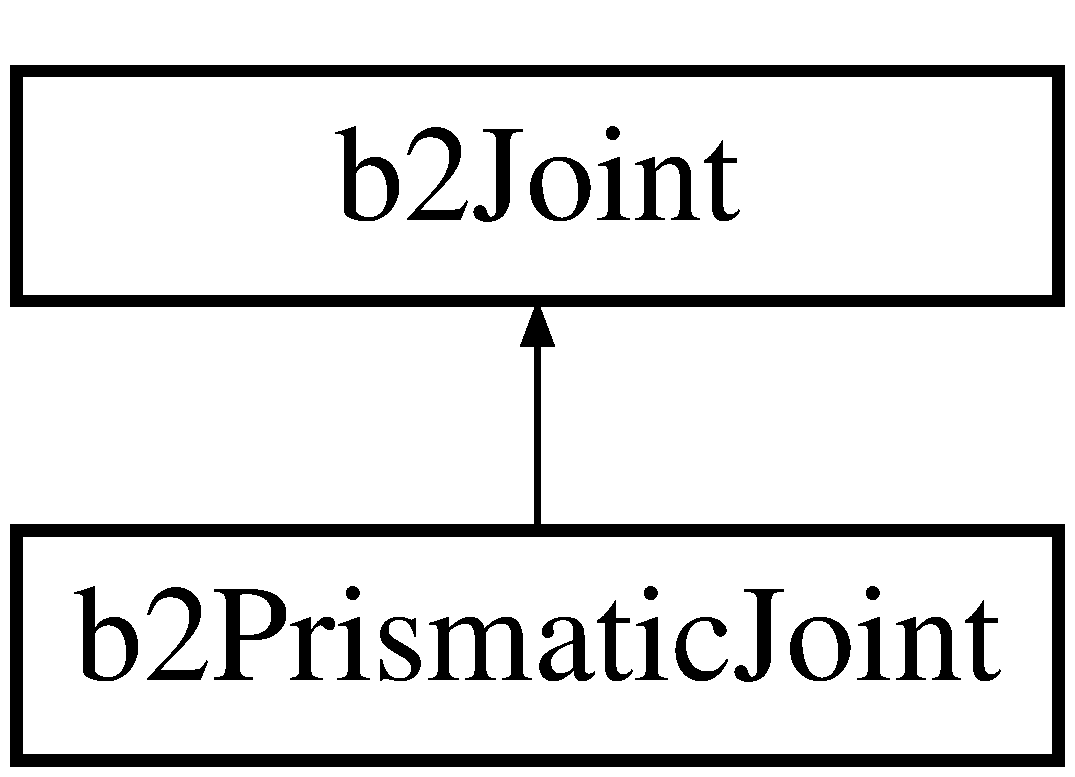
\includegraphics[height=2.000000cm]{classb2PrismaticJoint}
\end{center}
\end{figure}
\subsection*{Public Member Functions}
\begin{DoxyCompactItemize}
\item 
\mbox{\Hypertarget{classb2PrismaticJoint_abb6649d2a18abb209f68d5255cd6c606}\label{classb2PrismaticJoint_abb6649d2a18abb209f68d5255cd6c606}} 
\mbox{\hyperlink{structb2Vec2}{b2\+Vec2}} \mbox{\hyperlink{classb2PrismaticJoint_abb6649d2a18abb209f68d5255cd6c606}{Get\+AnchorA}} () const override
\begin{DoxyCompactList}\small\item\em Get the anchor point on bodyA in world coordinates. \end{DoxyCompactList}\item 
\mbox{\Hypertarget{classb2PrismaticJoint_a7e1d328bfd05895fd228c07bac41b9e5}\label{classb2PrismaticJoint_a7e1d328bfd05895fd228c07bac41b9e5}} 
\mbox{\hyperlink{structb2Vec2}{b2\+Vec2}} \mbox{\hyperlink{classb2PrismaticJoint_a7e1d328bfd05895fd228c07bac41b9e5}{Get\+AnchorB}} () const override
\begin{DoxyCompactList}\small\item\em Get the anchor point on bodyB in world coordinates. \end{DoxyCompactList}\item 
\mbox{\Hypertarget{classb2PrismaticJoint_ad73abb0ea7e316e863c35f4179ebc7ab}\label{classb2PrismaticJoint_ad73abb0ea7e316e863c35f4179ebc7ab}} 
\mbox{\hyperlink{structb2Vec2}{b2\+Vec2}} \mbox{\hyperlink{classb2PrismaticJoint_ad73abb0ea7e316e863c35f4179ebc7ab}{Get\+Reaction\+Force}} (float32 inv\+\_\+dt) const override
\begin{DoxyCompactList}\small\item\em Get the reaction force on bodyB at the joint anchor in Newtons. \end{DoxyCompactList}\item 
\mbox{\Hypertarget{classb2PrismaticJoint_a009526663c2ad848084103470375dc67}\label{classb2PrismaticJoint_a009526663c2ad848084103470375dc67}} 
float32 \mbox{\hyperlink{classb2PrismaticJoint_a009526663c2ad848084103470375dc67}{Get\+Reaction\+Torque}} (float32 inv\+\_\+dt) const override
\begin{DoxyCompactList}\small\item\em Get the reaction torque on bodyB in N$\ast$m. \end{DoxyCompactList}\item 
\mbox{\Hypertarget{classb2PrismaticJoint_a0a4812486867f4c7507bb8c29e860997}\label{classb2PrismaticJoint_a0a4812486867f4c7507bb8c29e860997}} 
const \mbox{\hyperlink{structb2Vec2}{b2\+Vec2}} \& \mbox{\hyperlink{classb2PrismaticJoint_a0a4812486867f4c7507bb8c29e860997}{Get\+Local\+AnchorA}} () const
\begin{DoxyCompactList}\small\item\em The local anchor point relative to bodyA\textquotesingle{}s origin. \end{DoxyCompactList}\item 
\mbox{\Hypertarget{classb2PrismaticJoint_ab9c2a0fbf075454320e87648750668b0}\label{classb2PrismaticJoint_ab9c2a0fbf075454320e87648750668b0}} 
const \mbox{\hyperlink{structb2Vec2}{b2\+Vec2}} \& \mbox{\hyperlink{classb2PrismaticJoint_ab9c2a0fbf075454320e87648750668b0}{Get\+Local\+AnchorB}} () const
\begin{DoxyCompactList}\small\item\em The local anchor point relative to bodyB\textquotesingle{}s origin. \end{DoxyCompactList}\item 
\mbox{\Hypertarget{classb2PrismaticJoint_a54d51d09f3c327c5c4238e054e2a3a76}\label{classb2PrismaticJoint_a54d51d09f3c327c5c4238e054e2a3a76}} 
const \mbox{\hyperlink{structb2Vec2}{b2\+Vec2}} \& \mbox{\hyperlink{classb2PrismaticJoint_a54d51d09f3c327c5c4238e054e2a3a76}{Get\+Local\+AxisA}} () const
\begin{DoxyCompactList}\small\item\em The local joint axis relative to bodyA. \end{DoxyCompactList}\item 
\mbox{\Hypertarget{classb2PrismaticJoint_a7b40d88d1bdb18089803d5abc6ba67c5}\label{classb2PrismaticJoint_a7b40d88d1bdb18089803d5abc6ba67c5}} 
float32 \mbox{\hyperlink{classb2PrismaticJoint_a7b40d88d1bdb18089803d5abc6ba67c5}{Get\+Reference\+Angle}} () const
\begin{DoxyCompactList}\small\item\em Get the reference angle. \end{DoxyCompactList}\item 
\mbox{\Hypertarget{classb2PrismaticJoint_abb008b99fb2df7357e6f3166d3c8b192}\label{classb2PrismaticJoint_abb008b99fb2df7357e6f3166d3c8b192}} 
float32 \mbox{\hyperlink{classb2PrismaticJoint_abb008b99fb2df7357e6f3166d3c8b192}{Get\+Joint\+Translation}} () const
\begin{DoxyCompactList}\small\item\em Get the current joint translation, usually in meters. \end{DoxyCompactList}\item 
\mbox{\Hypertarget{classb2PrismaticJoint_af407d14ac024abdee49b852613f1bbc2}\label{classb2PrismaticJoint_af407d14ac024abdee49b852613f1bbc2}} 
float32 \mbox{\hyperlink{classb2PrismaticJoint_af407d14ac024abdee49b852613f1bbc2}{Get\+Joint\+Speed}} () const
\begin{DoxyCompactList}\small\item\em Get the current joint translation speed, usually in meters per second. \end{DoxyCompactList}\item 
\mbox{\Hypertarget{classb2PrismaticJoint_a22e2442a17832f718447c63c9c6263c8}\label{classb2PrismaticJoint_a22e2442a17832f718447c63c9c6263c8}} 
bool \mbox{\hyperlink{classb2PrismaticJoint_a22e2442a17832f718447c63c9c6263c8}{Is\+Limit\+Enabled}} () const
\begin{DoxyCompactList}\small\item\em Is the joint limit enabled? \end{DoxyCompactList}\item 
\mbox{\Hypertarget{classb2PrismaticJoint_a6d419afe7bd4b0e36d2e4607df7f79f2}\label{classb2PrismaticJoint_a6d419afe7bd4b0e36d2e4607df7f79f2}} 
void \mbox{\hyperlink{classb2PrismaticJoint_a6d419afe7bd4b0e36d2e4607df7f79f2}{Enable\+Limit}} (bool flag)
\begin{DoxyCompactList}\small\item\em Enable/disable the joint limit. \end{DoxyCompactList}\item 
\mbox{\Hypertarget{classb2PrismaticJoint_a10a2d3c03164190d279fa3c72eafb49e}\label{classb2PrismaticJoint_a10a2d3c03164190d279fa3c72eafb49e}} 
float32 \mbox{\hyperlink{classb2PrismaticJoint_a10a2d3c03164190d279fa3c72eafb49e}{Get\+Lower\+Limit}} () const
\begin{DoxyCompactList}\small\item\em Get the lower joint limit, usually in meters. \end{DoxyCompactList}\item 
\mbox{\Hypertarget{classb2PrismaticJoint_aabae1da55e500b9c77007de4d085ffda}\label{classb2PrismaticJoint_aabae1da55e500b9c77007de4d085ffda}} 
float32 \mbox{\hyperlink{classb2PrismaticJoint_aabae1da55e500b9c77007de4d085ffda}{Get\+Upper\+Limit}} () const
\begin{DoxyCompactList}\small\item\em Get the upper joint limit, usually in meters. \end{DoxyCompactList}\item 
\mbox{\Hypertarget{classb2PrismaticJoint_a82a220e6d5a212c1924882e0855b0bef}\label{classb2PrismaticJoint_a82a220e6d5a212c1924882e0855b0bef}} 
void \mbox{\hyperlink{classb2PrismaticJoint_a82a220e6d5a212c1924882e0855b0bef}{Set\+Limits}} (float32 lower, float32 upper)
\begin{DoxyCompactList}\small\item\em Set the joint limits, usually in meters. \end{DoxyCompactList}\item 
\mbox{\Hypertarget{classb2PrismaticJoint_a06492dabf33439efdebceb29899c7fc9}\label{classb2PrismaticJoint_a06492dabf33439efdebceb29899c7fc9}} 
bool \mbox{\hyperlink{classb2PrismaticJoint_a06492dabf33439efdebceb29899c7fc9}{Is\+Motor\+Enabled}} () const
\begin{DoxyCompactList}\small\item\em Is the joint motor enabled? \end{DoxyCompactList}\item 
\mbox{\Hypertarget{classb2PrismaticJoint_a4a7fd079de49f7ed5aa4a5d8d90be2a2}\label{classb2PrismaticJoint_a4a7fd079de49f7ed5aa4a5d8d90be2a2}} 
void \mbox{\hyperlink{classb2PrismaticJoint_a4a7fd079de49f7ed5aa4a5d8d90be2a2}{Enable\+Motor}} (bool flag)
\begin{DoxyCompactList}\small\item\em Enable/disable the joint motor. \end{DoxyCompactList}\item 
\mbox{\Hypertarget{classb2PrismaticJoint_a602ef7a6ca4fca55d011f1b38ab5a6c3}\label{classb2PrismaticJoint_a602ef7a6ca4fca55d011f1b38ab5a6c3}} 
void \mbox{\hyperlink{classb2PrismaticJoint_a602ef7a6ca4fca55d011f1b38ab5a6c3}{Set\+Motor\+Speed}} (float32 speed)
\begin{DoxyCompactList}\small\item\em Set the motor speed, usually in meters per second. \end{DoxyCompactList}\item 
\mbox{\Hypertarget{classb2PrismaticJoint_a869c6edeb62ed01237b2adb09da273ae}\label{classb2PrismaticJoint_a869c6edeb62ed01237b2adb09da273ae}} 
float32 \mbox{\hyperlink{classb2PrismaticJoint_a869c6edeb62ed01237b2adb09da273ae}{Get\+Motor\+Speed}} () const
\begin{DoxyCompactList}\small\item\em Get the motor speed, usually in meters per second. \end{DoxyCompactList}\item 
\mbox{\Hypertarget{classb2PrismaticJoint_aa7817474aef15ca4815341479ac590e2}\label{classb2PrismaticJoint_aa7817474aef15ca4815341479ac590e2}} 
void \mbox{\hyperlink{classb2PrismaticJoint_aa7817474aef15ca4815341479ac590e2}{Set\+Max\+Motor\+Force}} (float32 force)
\begin{DoxyCompactList}\small\item\em Set the maximum motor force, usually in N. \end{DoxyCompactList}\item 
\mbox{\Hypertarget{classb2PrismaticJoint_aea8d0701bdf00a38fd2f24d94ae74842}\label{classb2PrismaticJoint_aea8d0701bdf00a38fd2f24d94ae74842}} 
float32 {\bfseries Get\+Max\+Motor\+Force} () const
\item 
\mbox{\Hypertarget{classb2PrismaticJoint_aaf7a7fe2300d9fe7a810306e9cfbb41a}\label{classb2PrismaticJoint_aaf7a7fe2300d9fe7a810306e9cfbb41a}} 
float32 \mbox{\hyperlink{classb2PrismaticJoint_aaf7a7fe2300d9fe7a810306e9cfbb41a}{Get\+Motor\+Force}} (float32 inv\+\_\+dt) const
\begin{DoxyCompactList}\small\item\em Get the current motor force given the inverse time step, usually in N. \end{DoxyCompactList}\item 
\mbox{\Hypertarget{classb2PrismaticJoint_a843ddb0f912085f3deb3ee7320d7ddc7}\label{classb2PrismaticJoint_a843ddb0f912085f3deb3ee7320d7ddc7}} 
void \mbox{\hyperlink{classb2PrismaticJoint_a843ddb0f912085f3deb3ee7320d7ddc7}{Dump}} () override
\begin{DoxyCompactList}\small\item\em Dump to b2\+Log. \end{DoxyCompactList}\end{DoxyCompactItemize}
\subsection*{Protected Member Functions}
\begin{DoxyCompactItemize}
\item 
\mbox{\Hypertarget{classb2PrismaticJoint_ab1586a2334f7e32137fbd7f807e249ca}\label{classb2PrismaticJoint_ab1586a2334f7e32137fbd7f807e249ca}} 
{\bfseries b2\+Prismatic\+Joint} (const \mbox{\hyperlink{structb2PrismaticJointDef}{b2\+Prismatic\+Joint\+Def}} $\ast$def)
\item 
\mbox{\Hypertarget{classb2PrismaticJoint_a840e9885d49bf621c46df79733df21dc}\label{classb2PrismaticJoint_a840e9885d49bf621c46df79733df21dc}} 
void {\bfseries Init\+Velocity\+Constraints} (const \mbox{\hyperlink{structb2SolverData}{b2\+Solver\+Data}} \&data) override
\item 
\mbox{\Hypertarget{classb2PrismaticJoint_a028c0ca03ca8437606d1175ca8de63d6}\label{classb2PrismaticJoint_a028c0ca03ca8437606d1175ca8de63d6}} 
void {\bfseries Solve\+Velocity\+Constraints} (const \mbox{\hyperlink{structb2SolverData}{b2\+Solver\+Data}} \&data) override
\item 
\mbox{\Hypertarget{classb2PrismaticJoint_ac841608a56e83f709e08b805ed8c92e3}\label{classb2PrismaticJoint_ac841608a56e83f709e08b805ed8c92e3}} 
bool {\bfseries Solve\+Position\+Constraints} (const \mbox{\hyperlink{structb2SolverData}{b2\+Solver\+Data}} \&data) override
\end{DoxyCompactItemize}
\subsection*{Protected Attributes}
\begin{DoxyCompactItemize}
\item 
\mbox{\Hypertarget{classb2PrismaticJoint_aeec29d80cc57252702fd645c31ca7889}\label{classb2PrismaticJoint_aeec29d80cc57252702fd645c31ca7889}} 
\mbox{\hyperlink{structb2Vec2}{b2\+Vec2}} {\bfseries m\+\_\+local\+AnchorA}
\item 
\mbox{\Hypertarget{classb2PrismaticJoint_ae9cb63f225e4b4dcc287ab475868d044}\label{classb2PrismaticJoint_ae9cb63f225e4b4dcc287ab475868d044}} 
\mbox{\hyperlink{structb2Vec2}{b2\+Vec2}} {\bfseries m\+\_\+local\+AnchorB}
\item 
\mbox{\Hypertarget{classb2PrismaticJoint_ab68f8bb2a8012e4646dc274db1723fbf}\label{classb2PrismaticJoint_ab68f8bb2a8012e4646dc274db1723fbf}} 
\mbox{\hyperlink{structb2Vec2}{b2\+Vec2}} {\bfseries m\+\_\+local\+X\+AxisA}
\item 
\mbox{\Hypertarget{classb2PrismaticJoint_a6885a7d60a2596883660183bcf721ea9}\label{classb2PrismaticJoint_a6885a7d60a2596883660183bcf721ea9}} 
\mbox{\hyperlink{structb2Vec2}{b2\+Vec2}} {\bfseries m\+\_\+local\+Y\+AxisA}
\item 
\mbox{\Hypertarget{classb2PrismaticJoint_ad8b2ee403ba7517966d9e05b988e28c6}\label{classb2PrismaticJoint_ad8b2ee403ba7517966d9e05b988e28c6}} 
float32 {\bfseries m\+\_\+reference\+Angle}
\item 
\mbox{\Hypertarget{classb2PrismaticJoint_a92530ae3ec9765d775ec82a39400f770}\label{classb2PrismaticJoint_a92530ae3ec9765d775ec82a39400f770}} 
\mbox{\hyperlink{structb2Vec3}{b2\+Vec3}} {\bfseries m\+\_\+impulse}
\item 
\mbox{\Hypertarget{classb2PrismaticJoint_aff90d55579b511950334d8a0449f1155}\label{classb2PrismaticJoint_aff90d55579b511950334d8a0449f1155}} 
float32 {\bfseries m\+\_\+motor\+Impulse}
\item 
\mbox{\Hypertarget{classb2PrismaticJoint_a82e13b09e43d0d82365845aa3fb7f9fe}\label{classb2PrismaticJoint_a82e13b09e43d0d82365845aa3fb7f9fe}} 
float32 {\bfseries m\+\_\+lower\+Translation}
\item 
\mbox{\Hypertarget{classb2PrismaticJoint_a09a5bbe1ae720f1f4e2b1fd16f8ad613}\label{classb2PrismaticJoint_a09a5bbe1ae720f1f4e2b1fd16f8ad613}} 
float32 {\bfseries m\+\_\+upper\+Translation}
\item 
\mbox{\Hypertarget{classb2PrismaticJoint_a42685bcbc18ea7a74d75c459a381a7b9}\label{classb2PrismaticJoint_a42685bcbc18ea7a74d75c459a381a7b9}} 
float32 {\bfseries m\+\_\+max\+Motor\+Force}
\item 
\mbox{\Hypertarget{classb2PrismaticJoint_a0851a1993e9e4f4103a8f7dbaeedb9c5}\label{classb2PrismaticJoint_a0851a1993e9e4f4103a8f7dbaeedb9c5}} 
float32 {\bfseries m\+\_\+motor\+Speed}
\item 
\mbox{\Hypertarget{classb2PrismaticJoint_ace469adee4132fb1de01fe5ab3d26389}\label{classb2PrismaticJoint_ace469adee4132fb1de01fe5ab3d26389}} 
bool {\bfseries m\+\_\+enable\+Limit}
\item 
\mbox{\Hypertarget{classb2PrismaticJoint_af36c993314f8ae833f5f3b3aebd66497}\label{classb2PrismaticJoint_af36c993314f8ae833f5f3b3aebd66497}} 
bool {\bfseries m\+\_\+enable\+Motor}
\item 
\mbox{\Hypertarget{classb2PrismaticJoint_ad5ce4e2d66a0d612573e07103b407b99}\label{classb2PrismaticJoint_ad5ce4e2d66a0d612573e07103b407b99}} 
b2\+Limit\+State {\bfseries m\+\_\+limit\+State}
\item 
\mbox{\Hypertarget{classb2PrismaticJoint_a2cd142bc49ea7eb475e0811f11932e64}\label{classb2PrismaticJoint_a2cd142bc49ea7eb475e0811f11932e64}} 
int32 {\bfseries m\+\_\+indexA}
\item 
\mbox{\Hypertarget{classb2PrismaticJoint_a6a555684a2112f2a2f4f0ab91a2b5ed4}\label{classb2PrismaticJoint_a6a555684a2112f2a2f4f0ab91a2b5ed4}} 
int32 {\bfseries m\+\_\+indexB}
\item 
\mbox{\Hypertarget{classb2PrismaticJoint_ad705cb8cdc92f23185e8f3af728bf0bb}\label{classb2PrismaticJoint_ad705cb8cdc92f23185e8f3af728bf0bb}} 
\mbox{\hyperlink{structb2Vec2}{b2\+Vec2}} {\bfseries m\+\_\+local\+CenterA}
\item 
\mbox{\Hypertarget{classb2PrismaticJoint_afd0f5412cb44f84a30224fbfedf7af84}\label{classb2PrismaticJoint_afd0f5412cb44f84a30224fbfedf7af84}} 
\mbox{\hyperlink{structb2Vec2}{b2\+Vec2}} {\bfseries m\+\_\+local\+CenterB}
\item 
\mbox{\Hypertarget{classb2PrismaticJoint_a1bc57bddac4dc8aa36c28ef7b7aaa235}\label{classb2PrismaticJoint_a1bc57bddac4dc8aa36c28ef7b7aaa235}} 
float32 {\bfseries m\+\_\+inv\+MassA}
\item 
\mbox{\Hypertarget{classb2PrismaticJoint_a51f64c912da93d306af94a3c55cef174}\label{classb2PrismaticJoint_a51f64c912da93d306af94a3c55cef174}} 
float32 {\bfseries m\+\_\+inv\+MassB}
\item 
\mbox{\Hypertarget{classb2PrismaticJoint_a75cae2a36290b6c19b732a997223b09a}\label{classb2PrismaticJoint_a75cae2a36290b6c19b732a997223b09a}} 
float32 {\bfseries m\+\_\+inv\+IA}
\item 
\mbox{\Hypertarget{classb2PrismaticJoint_ac3ac47948a3f9ca1002449cd3112eb5f}\label{classb2PrismaticJoint_ac3ac47948a3f9ca1002449cd3112eb5f}} 
float32 {\bfseries m\+\_\+inv\+IB}
\item 
\mbox{\Hypertarget{classb2PrismaticJoint_af487c98feb16d19d5d1b320ad2aefb49}\label{classb2PrismaticJoint_af487c98feb16d19d5d1b320ad2aefb49}} 
\mbox{\hyperlink{structb2Vec2}{b2\+Vec2}} {\bfseries m\+\_\+axis}
\item 
\mbox{\Hypertarget{classb2PrismaticJoint_a560f7177fbc3db1916e076a755b406e5}\label{classb2PrismaticJoint_a560f7177fbc3db1916e076a755b406e5}} 
\mbox{\hyperlink{structb2Vec2}{b2\+Vec2}} {\bfseries m\+\_\+perp}
\item 
\mbox{\Hypertarget{classb2PrismaticJoint_a5dad08589b72d49c05b61bbee0a1fa39}\label{classb2PrismaticJoint_a5dad08589b72d49c05b61bbee0a1fa39}} 
float32 {\bfseries m\+\_\+s1}
\item 
\mbox{\Hypertarget{classb2PrismaticJoint_a7b82750572655292a3e08490d1131f31}\label{classb2PrismaticJoint_a7b82750572655292a3e08490d1131f31}} 
float32 {\bfseries m\+\_\+s2}
\item 
\mbox{\Hypertarget{classb2PrismaticJoint_afa9f7a7b4317a491d76390e0db7034e4}\label{classb2PrismaticJoint_afa9f7a7b4317a491d76390e0db7034e4}} 
float32 {\bfseries m\+\_\+a1}
\item 
\mbox{\Hypertarget{classb2PrismaticJoint_a91fd8e15cd9c610c343d162cb31e6552}\label{classb2PrismaticJoint_a91fd8e15cd9c610c343d162cb31e6552}} 
float32 {\bfseries m\+\_\+a2}
\item 
\mbox{\Hypertarget{classb2PrismaticJoint_a2a19322c65fd08eda34991dfa50c5d00}\label{classb2PrismaticJoint_a2a19322c65fd08eda34991dfa50c5d00}} 
\mbox{\hyperlink{structb2Mat33}{b2\+Mat33}} {\bfseries m\+\_\+K}
\item 
\mbox{\Hypertarget{classb2PrismaticJoint_a6e9fcd93328657df8b7fa1c6c6a517dd}\label{classb2PrismaticJoint_a6e9fcd93328657df8b7fa1c6c6a517dd}} 
float32 {\bfseries m\+\_\+motor\+Mass}
\end{DoxyCompactItemize}
\subsection*{Friends}
\begin{DoxyCompactItemize}
\item 
\mbox{\Hypertarget{classb2PrismaticJoint_a54ade8ed3d794298108d7f4c4e4793fa}\label{classb2PrismaticJoint_a54ade8ed3d794298108d7f4c4e4793fa}} 
class {\bfseries b2\+Joint}
\item 
\mbox{\Hypertarget{classb2PrismaticJoint_a13c275221e30bb485e17e4e04553cb71}\label{classb2PrismaticJoint_a13c275221e30bb485e17e4e04553cb71}} 
class {\bfseries b2\+Gear\+Joint}
\end{DoxyCompactItemize}
\subsection*{Additional Inherited Members}


\subsection{Detailed Description}
A prismatic joint. This joint provides one degree of freedom\+: translation along an axis fixed in bodyA. Relative rotation is prevented. You can use a joint limit to restrict the range of motion and a joint motor to drive the motion or to model joint friction. 

The documentation for this class was generated from the following files\+:\begin{DoxyCompactItemize}
\item 
Dynamics/\+Joints/b2\+Prismatic\+Joint.\+h\item 
Dynamics/\+Joints/b2\+Prismatic\+Joint.\+cpp\end{DoxyCompactItemize}

\hypertarget{structb2PrismaticJointDef}{}\section{b2\+Prismatic\+Joint\+Def Struct Reference}
\label{structb2PrismaticJointDef}\index{b2\+Prismatic\+Joint\+Def@{b2\+Prismatic\+Joint\+Def}}


{\ttfamily \#include $<$b2\+Prismatic\+Joint.\+h$>$}

Inheritance diagram for b2\+Prismatic\+Joint\+Def\+:\begin{figure}[H]
\begin{center}
\leavevmode
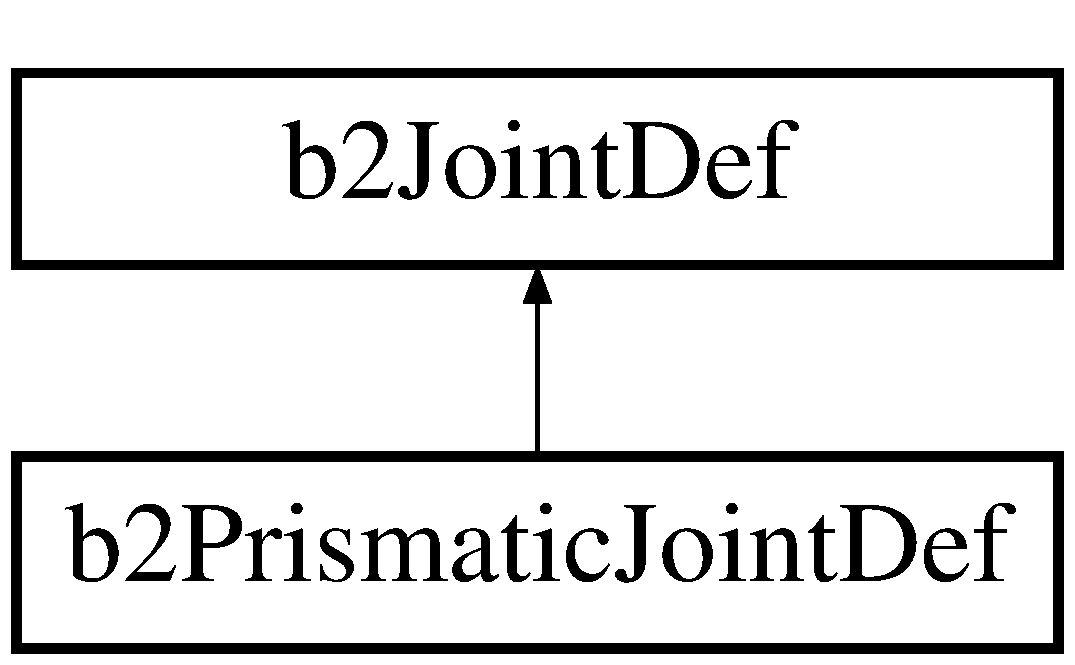
\includegraphics[height=2.000000cm]{structb2PrismaticJointDef}
\end{center}
\end{figure}
\subsection*{Public Member Functions}
\begin{DoxyCompactItemize}
\item 
void \mbox{\hyperlink{structb2PrismaticJointDef_ae60043bc22b077e8c59ab248dc34652f}{Initialize}} (\mbox{\hyperlink{classb2Body}{b2\+Body}} $\ast$\mbox{\hyperlink{structb2JointDef_a8cd54c93da396be75a9788f2c6897f05}{bodyA}}, \mbox{\hyperlink{classb2Body}{b2\+Body}} $\ast$\mbox{\hyperlink{structb2JointDef_aa4f4dee2fbcd12187b19506b60e68e3d}{bodyB}}, const \mbox{\hyperlink{structb2Vec2}{b2\+Vec2}} \&anchor, const \mbox{\hyperlink{structb2Vec2}{b2\+Vec2}} \&axis)
\end{DoxyCompactItemize}
\subsection*{Public Attributes}
\begin{DoxyCompactItemize}
\item 
\mbox{\Hypertarget{structb2PrismaticJointDef_abb51df8daff7a55f47adc83e4f7fa5b9}\label{structb2PrismaticJointDef_abb51df8daff7a55f47adc83e4f7fa5b9}} 
\mbox{\hyperlink{structb2Vec2}{b2\+Vec2}} \mbox{\hyperlink{structb2PrismaticJointDef_abb51df8daff7a55f47adc83e4f7fa5b9}{local\+AnchorA}}
\begin{DoxyCompactList}\small\item\em The local anchor point relative to bodyA\textquotesingle{}s origin. \end{DoxyCompactList}\item 
\mbox{\Hypertarget{structb2PrismaticJointDef_a5acc1f2f14d1b659fc9d804ab1baf4a3}\label{structb2PrismaticJointDef_a5acc1f2f14d1b659fc9d804ab1baf4a3}} 
\mbox{\hyperlink{structb2Vec2}{b2\+Vec2}} \mbox{\hyperlink{structb2PrismaticJointDef_a5acc1f2f14d1b659fc9d804ab1baf4a3}{local\+AnchorB}}
\begin{DoxyCompactList}\small\item\em The local anchor point relative to bodyB\textquotesingle{}s origin. \end{DoxyCompactList}\item 
\mbox{\Hypertarget{structb2PrismaticJointDef_af36fdbcedca5a392a2649cd235c42676}\label{structb2PrismaticJointDef_af36fdbcedca5a392a2649cd235c42676}} 
\mbox{\hyperlink{structb2Vec2}{b2\+Vec2}} \mbox{\hyperlink{structb2PrismaticJointDef_af36fdbcedca5a392a2649cd235c42676}{local\+AxisA}}
\begin{DoxyCompactList}\small\item\em The local translation unit axis in bodyA. \end{DoxyCompactList}\item 
\mbox{\Hypertarget{structb2PrismaticJointDef_aa84b43d08e6e11b4daa0c86f46094463}\label{structb2PrismaticJointDef_aa84b43d08e6e11b4daa0c86f46094463}} 
float32 \mbox{\hyperlink{structb2PrismaticJointDef_aa84b43d08e6e11b4daa0c86f46094463}{reference\+Angle}}
\begin{DoxyCompactList}\small\item\em The constrained angle between the bodies\+: body\+B\+\_\+angle -\/ _body\+A\+\_\+angle. \end{DoxyCompactList}\item
\mbox{\Hypertarget{structb2PrismaticJointDef_aa61a03b68caac62a5cf66354f6756eae}\label{structb2PrismaticJointDef_aa61a03b68caac62a5cf66354f6756eae}} 
bool \mbox{\hyperlink{structb2PrismaticJointDef_aa61a03b68caac62a5cf66354f6756eae}{enable\+Limit}}
\begin{DoxyCompactList}\small\item\em Enable/disable the joint limit. \end{DoxyCompactList}\item 
\mbox{\Hypertarget{structb2PrismaticJointDef_ac0a0e2a669d640ebea354895fe6a9fb6}\label{structb2PrismaticJointDef_ac0a0e2a669d640ebea354895fe6a9fb6}} 
float32 \mbox{\hyperlink{structb2PrismaticJointDef_ac0a0e2a669d640ebea354895fe6a9fb6}{lower\+Translation}}
\begin{DoxyCompactList}\small\item\em The lower translation limit, usually in meters. \end{DoxyCompactList}\item 
\mbox{\Hypertarget{structb2PrismaticJointDef_ae3eac123c7fe543071bdfcd1a6942350}\label{structb2PrismaticJointDef_ae3eac123c7fe543071bdfcd1a6942350}} 
float32 \mbox{\hyperlink{structb2PrismaticJointDef_ae3eac123c7fe543071bdfcd1a6942350}{upper\+Translation}}
\begin{DoxyCompactList}\small\item\em The upper translation limit, usually in meters. \end{DoxyCompactList}\item 
\mbox{\Hypertarget{structb2PrismaticJointDef_a58ac79a54a8110d3a745e1d6d36990dc}\label{structb2PrismaticJointDef_a58ac79a54a8110d3a745e1d6d36990dc}} 
bool \mbox{\hyperlink{structb2PrismaticJointDef_a58ac79a54a8110d3a745e1d6d36990dc}{enable\+Motor}}
\begin{DoxyCompactList}\small\item\em Enable/disable the joint motor. \end{DoxyCompactList}\item 
\mbox{\Hypertarget{structb2PrismaticJointDef_aabeec48af1e49c7f9fed5e0bc8270a1b}\label{structb2PrismaticJointDef_aabeec48af1e49c7f9fed5e0bc8270a1b}} 
float32 \mbox{\hyperlink{structb2PrismaticJointDef_aabeec48af1e49c7f9fed5e0bc8270a1b}{max\+Motor\+Force}}
\begin{DoxyCompactList}\small\item\em The maximum motor torque, usually in N-\/m. \end{DoxyCompactList}\item 
\mbox{\Hypertarget{structb2PrismaticJointDef_ac4bdaea15653657e724a04fc60f3f235}\label{structb2PrismaticJointDef_ac4bdaea15653657e724a04fc60f3f235}} 
float32 \mbox{\hyperlink{structb2PrismaticJointDef_ac4bdaea15653657e724a04fc60f3f235}{motor\+Speed}}
\begin{DoxyCompactList}\small\item\em The desired motor speed in radians per second. \end{DoxyCompactList}\end{DoxyCompactItemize}


\subsection{Detailed Description}
Prismatic joint definition. This requires defining a line of motion using an axis and an anchor point. The definition uses local anchor points and a local axis so that the initial configuration can violate the constraint slightly. The joint translation is zero when the local anchor points coincide in world space. Using local anchors and a local axis helps when saving and loading a game. 

\subsection{Member Function Documentation}
\mbox{\Hypertarget{structb2PrismaticJointDef_ae60043bc22b077e8c59ab248dc34652f}\label{structb2PrismaticJointDef_ae60043bc22b077e8c59ab248dc34652f}} 
\index{b2\+Prismatic\+Joint\+Def@{b2\+Prismatic\+Joint\+Def}!Initialize@{Initialize}}
\index{Initialize@{Initialize}!b2\+Prismatic\+Joint\+Def@{b2\+Prismatic\+Joint\+Def}}
\subsubsection{\texorpdfstring{Initialize()}{Initialize()}}
{\footnotesize\ttfamily void b2\+Prismatic\+Joint\+Def\+::\+Initialize (\begin{DoxyParamCaption}\item[{\mbox{\hyperlink{classb2Body}{b2\+Body}} $\ast$}]{bodyA,  }\item[{\mbox{\hyperlink{classb2Body}{b2\+Body}} $\ast$}]{bodyB,  }\item[{const \mbox{\hyperlink{structb2Vec2}{b2\+Vec2}} \&}]{anchor,  }\item[{const \mbox{\hyperlink{structb2Vec2}{b2\+Vec2}} \&}]{axis }\end{DoxyParamCaption})}

Initialize the bodies, anchors, axis, and reference angle using the world anchor and unit world axis. 

The documentation for this struct was generated from the following files\+:\begin{DoxyCompactItemize}
\item 
Dynamics/\+Joints/b2\+Prismatic\+Joint.\+h\item 
Dynamics/\+Joints/b2\+Prismatic\+Joint.\+cpp\end{DoxyCompactItemize}

\hypertarget{structb2Profile}{}\section{b2\+Profile Struct Reference}
\label{structb2Profile}\index{b2\+Profile@{b2\+Profile}}


Profiling data. Times are in milliseconds.  




{\ttfamily \#include $<$b2\+Time\+Step.\+h$>$}

\subsection*{Public Attributes}
\begin{DoxyCompactItemize}
\item 
\mbox{\Hypertarget{structb2Profile_a5b93de1d56902224868beacc478b9863}\label{structb2Profile_a5b93de1d56902224868beacc478b9863}} 
float32 {\bfseries step}
\item 
\mbox{\Hypertarget{structb2Profile_af827d9e54f7a4e94d0a023e18466b960}\label{structb2Profile_af827d9e54f7a4e94d0a023e18466b960}} 
float32 {\bfseries collide}
\item 
\mbox{\Hypertarget{structb2Profile_afbefc05f05ec8bfd6cb2011929688a0b}\label{structb2Profile_afbefc05f05ec8bfd6cb2011929688a0b}} 
float32 {\bfseries solve}
\item 
\mbox{\Hypertarget{structb2Profile_a010110900c27ccc88cd5e23b0e12e96e}\label{structb2Profile_a010110900c27ccc88cd5e23b0e12e96e}} 
float32 {\bfseries solve\+Init}
\item 
\mbox{\Hypertarget{structb2Profile_ae4d29a19b38de81621bccdbf75595233}\label{structb2Profile_ae4d29a19b38de81621bccdbf75595233}} 
float32 {\bfseries solve\+Velocity}
\item 
\mbox{\Hypertarget{structb2Profile_a78e22d104226863492ebab9ea30a9ed9}\label{structb2Profile_a78e22d104226863492ebab9ea30a9ed9}} 
float32 {\bfseries solve\+Position}
\item 
\mbox{\Hypertarget{structb2Profile_a6bd556e43a6fa3853adad9fd71e56b44}\label{structb2Profile_a6bd556e43a6fa3853adad9fd71e56b44}} 
float32 {\bfseries broadphase}
\item 
\mbox{\Hypertarget{structb2Profile_a74e8ea0c6ca39250d639ec94b69a803e}\label{structb2Profile_a74e8ea0c6ca39250d639ec94b69a803e}} 
float32 {\bfseries solve\+T\+OI}
\end{DoxyCompactItemize}


\subsection{Detailed Description}
Profiling data. Times are in milliseconds. 

The documentation for this struct was generated from the following file\+:\begin{DoxyCompactItemize}
\item 
Dynamics/b2\+Time\+Step.\+h\end{DoxyCompactItemize}

\hypertarget{classb2PulleyJoint}{}\section{b2\+Pulley\+Joint Class Reference}
\label{classb2PulleyJoint}\index{b2\+Pulley\+Joint@{b2\+Pulley\+Joint}}


{\ttfamily \#include $<$b2\+Pulley\+Joint.\+h$>$}

Inheritance diagram for b2\+Pulley\+Joint\+:\begin{figure}[H]
\begin{center}
\leavevmode
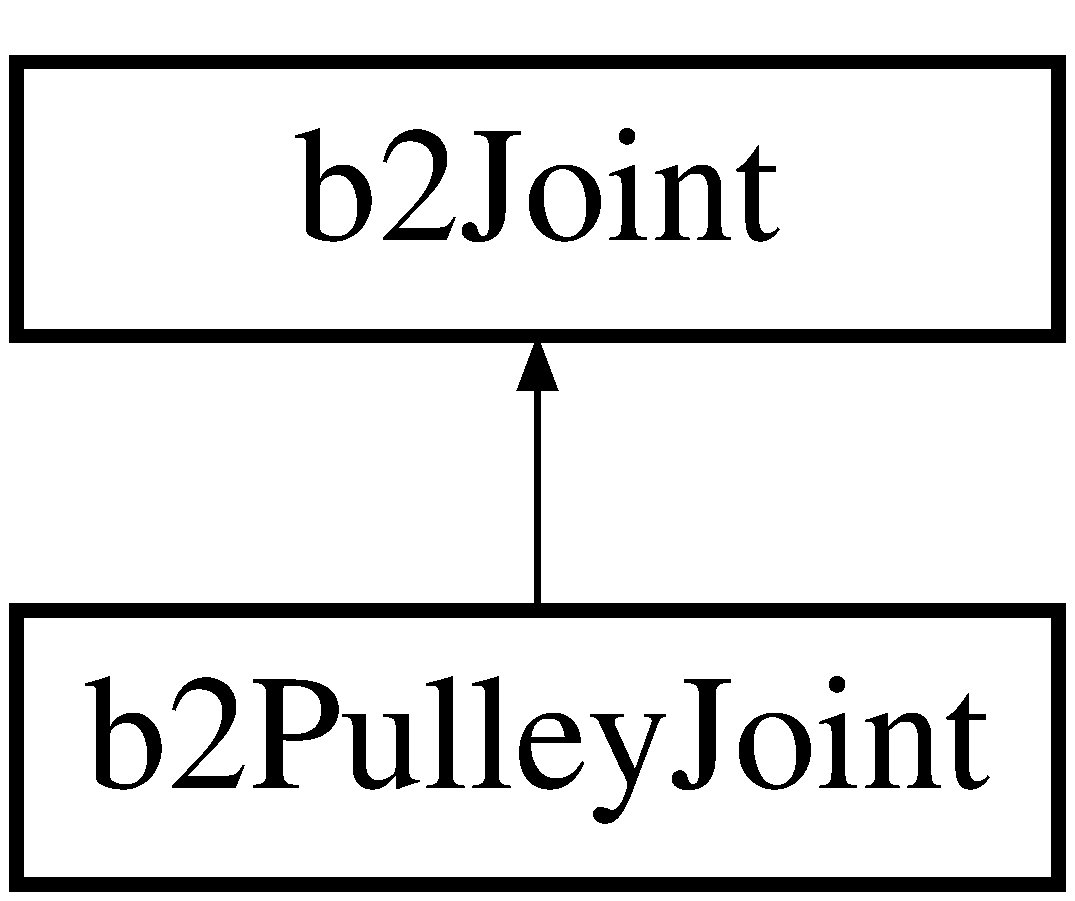
\includegraphics[height=2.000000cm]{classb2PulleyJoint}
\end{center}
\end{figure}
\subsection*{Public Member Functions}
\begin{DoxyCompactItemize}
\item 
\mbox{\Hypertarget{classb2PulleyJoint_af7167643e6d72d879eea619a368194c1}\label{classb2PulleyJoint_af7167643e6d72d879eea619a368194c1}} 
\mbox{\hyperlink{structb2Vec2}{b2\+Vec2}} \mbox{\hyperlink{classb2PulleyJoint_af7167643e6d72d879eea619a368194c1}{Get\+AnchorA}} () const override
\begin{DoxyCompactList}\small\item\em Get the anchor point on bodyA in world coordinates. \end{DoxyCompactList}\item 
\mbox{\Hypertarget{classb2PulleyJoint_aee56f103c1d1d30fcbd3a8570e321ba9}\label{classb2PulleyJoint_aee56f103c1d1d30fcbd3a8570e321ba9}} 
\mbox{\hyperlink{structb2Vec2}{b2\+Vec2}} \mbox{\hyperlink{classb2PulleyJoint_aee56f103c1d1d30fcbd3a8570e321ba9}{Get\+AnchorB}} () const override
\begin{DoxyCompactList}\small\item\em Get the anchor point on bodyB in world coordinates. \end{DoxyCompactList}\item 
\mbox{\Hypertarget{classb2PulleyJoint_a90904a458169a22fe0a9e2c4f5332101}\label{classb2PulleyJoint_a90904a458169a22fe0a9e2c4f5332101}} 
\mbox{\hyperlink{structb2Vec2}{b2\+Vec2}} \mbox{\hyperlink{classb2PulleyJoint_a90904a458169a22fe0a9e2c4f5332101}{Get\+Reaction\+Force}} (float32 inv\+\_\+dt) const override
\begin{DoxyCompactList}\small\item\em Get the reaction force on bodyB at the joint anchor in Newtons. \end{DoxyCompactList}\item 
\mbox{\Hypertarget{classb2PulleyJoint_a707bed4e4541d5da58022a6ee2bc58a1}\label{classb2PulleyJoint_a707bed4e4541d5da58022a6ee2bc58a1}} 
float32 \mbox{\hyperlink{classb2PulleyJoint_a707bed4e4541d5da58022a6ee2bc58a1}{Get\+Reaction\+Torque}} (float32 inv\+\_\+dt) const override
\begin{DoxyCompactList}\small\item\em Get the reaction torque on bodyB in N$\ast$m. \end{DoxyCompactList}\item 
\mbox{\Hypertarget{classb2PulleyJoint_a082db0a3ab20f682b9c7d5f41f0cc79e}\label{classb2PulleyJoint_a082db0a3ab20f682b9c7d5f41f0cc79e}} 
\mbox{\hyperlink{structb2Vec2}{b2\+Vec2}} \mbox{\hyperlink{classb2PulleyJoint_a082db0a3ab20f682b9c7d5f41f0cc79e}{Get\+Ground\+AnchorA}} () const
\begin{DoxyCompactList}\small\item\em Get the first ground anchor. \end{DoxyCompactList}\item 
\mbox{\Hypertarget{classb2PulleyJoint_afb105270ab46c3fc3f862cab6e127971}\label{classb2PulleyJoint_afb105270ab46c3fc3f862cab6e127971}} 
\mbox{\hyperlink{structb2Vec2}{b2\+Vec2}} \mbox{\hyperlink{classb2PulleyJoint_afb105270ab46c3fc3f862cab6e127971}{Get\+Ground\+AnchorB}} () const
\begin{DoxyCompactList}\small\item\em Get the second ground anchor. \end{DoxyCompactList}\item 
\mbox{\Hypertarget{classb2PulleyJoint_ac92d5def8d6d14777b255cbeea6b9c30}\label{classb2PulleyJoint_ac92d5def8d6d14777b255cbeea6b9c30}} 
float32 \mbox{\hyperlink{classb2PulleyJoint_ac92d5def8d6d14777b255cbeea6b9c30}{Get\+LengthA}} () const
\begin{DoxyCompactList}\small\item\em Get the current length of the segment attached to bodyA. \end{DoxyCompactList}\item 
\mbox{\Hypertarget{classb2PulleyJoint_a8558201dc81ba177f040ec7e12d78c8d}\label{classb2PulleyJoint_a8558201dc81ba177f040ec7e12d78c8d}} 
float32 \mbox{\hyperlink{classb2PulleyJoint_a8558201dc81ba177f040ec7e12d78c8d}{Get\+LengthB}} () const
\begin{DoxyCompactList}\small\item\em Get the current length of the segment attached to bodyB. \end{DoxyCompactList}\item 
\mbox{\Hypertarget{classb2PulleyJoint_a130e85a48bfe54588d15766b94e3b2b2}\label{classb2PulleyJoint_a130e85a48bfe54588d15766b94e3b2b2}} 
float32 \mbox{\hyperlink{classb2PulleyJoint_a130e85a48bfe54588d15766b94e3b2b2}{Get\+Ratio}} () const
\begin{DoxyCompactList}\small\item\em Get the pulley ratio. \end{DoxyCompactList}\item 
\mbox{\Hypertarget{classb2PulleyJoint_a4b4f29d81b7d2ffdda5af2f588f49ab6}\label{classb2PulleyJoint_a4b4f29d81b7d2ffdda5af2f588f49ab6}} 
float32 \mbox{\hyperlink{classb2PulleyJoint_a4b4f29d81b7d2ffdda5af2f588f49ab6}{Get\+Current\+LengthA}} () const
\begin{DoxyCompactList}\small\item\em Get the current length of the segment attached to bodyA. \end{DoxyCompactList}\item 
\mbox{\Hypertarget{classb2PulleyJoint_aa2d15dc26b2df0a446ccda652058085d}\label{classb2PulleyJoint_aa2d15dc26b2df0a446ccda652058085d}} 
float32 \mbox{\hyperlink{classb2PulleyJoint_aa2d15dc26b2df0a446ccda652058085d}{Get\+Current\+LengthB}} () const
\begin{DoxyCompactList}\small\item\em Get the current length of the segment attached to bodyB. \end{DoxyCompactList}\item 
\mbox{\Hypertarget{classb2PulleyJoint_a51b3fa745fc43f806cee1328099b4623}\label{classb2PulleyJoint_a51b3fa745fc43f806cee1328099b4623}} 
void \mbox{\hyperlink{classb2PulleyJoint_a51b3fa745fc43f806cee1328099b4623}{Dump}} () override
\begin{DoxyCompactList}\small\item\em Dump joint to dm\+Log. \end{DoxyCompactList}\item 
\mbox{\Hypertarget{classb2PulleyJoint_a5a9e626c758380fe565837bedb3dc018}\label{classb2PulleyJoint_a5a9e626c758380fe565837bedb3dc018}} 
void \mbox{\hyperlink{classb2PulleyJoint_a5a9e626c758380fe565837bedb3dc018}{Shift\+Origin}} (const \mbox{\hyperlink{structb2Vec2}{b2\+Vec2}} \&new\+Origin) override
\begin{DoxyCompactList}\small\item\em Implement \mbox{\hyperlink{classb2Joint_a7804f649e993dc0fd9ae47fde5601f90}{b2\+Joint\+::\+Shift\+Origin}}. \end{DoxyCompactList}\end{DoxyCompactItemize}
\subsection*{Protected Member Functions}
\begin{DoxyCompactItemize}
\item 
\mbox{\Hypertarget{classb2PulleyJoint_aca1b8dc6fb05c134ccbc0423674c1867}\label{classb2PulleyJoint_aca1b8dc6fb05c134ccbc0423674c1867}} 
{\bfseries b2\+Pulley\+Joint} (const \mbox{\hyperlink{structb2PulleyJointDef}{b2\+Pulley\+Joint\+Def}} $\ast$data)
\item 
\mbox{\Hypertarget{classb2PulleyJoint_a1826611f1dfe6284c3ce3afdab875e94}\label{classb2PulleyJoint_a1826611f1dfe6284c3ce3afdab875e94}} 
void {\bfseries Init\+Velocity\+Constraints} (const \mbox{\hyperlink{structb2SolverData}{b2\+Solver\+Data}} \&data) override
\item 
\mbox{\Hypertarget{classb2PulleyJoint_a80de874e392a8238fd2e965f5080222b}\label{classb2PulleyJoint_a80de874e392a8238fd2e965f5080222b}} 
void {\bfseries Solve\+Velocity\+Constraints} (const \mbox{\hyperlink{structb2SolverData}{b2\+Solver\+Data}} \&data) override
\item 
\mbox{\Hypertarget{classb2PulleyJoint_ac3d5f78f3bdd248ca368add8f21b7e95}\label{classb2PulleyJoint_ac3d5f78f3bdd248ca368add8f21b7e95}} 
bool {\bfseries Solve\+Position\+Constraints} (const \mbox{\hyperlink{structb2SolverData}{b2\+Solver\+Data}} \&data) override
\end{DoxyCompactItemize}
\subsection*{Protected Attributes}
\begin{DoxyCompactItemize}
\item 
\mbox{\Hypertarget{classb2PulleyJoint_a13456d1c62a4e96e8247988152be4166}\label{classb2PulleyJoint_a13456d1c62a4e96e8247988152be4166}} 
\mbox{\hyperlink{structb2Vec2}{b2\+Vec2}} {\bfseries m\+\_\+ground\+AnchorA}
\item 
\mbox{\Hypertarget{classb2PulleyJoint_a9cc8195bf4e2d53606db0b49d9fc1cbc}\label{classb2PulleyJoint_a9cc8195bf4e2d53606db0b49d9fc1cbc}} 
\mbox{\hyperlink{structb2Vec2}{b2\+Vec2}} {\bfseries m\+\_\+ground\+AnchorB}
\item 
\mbox{\Hypertarget{classb2PulleyJoint_a26f2565f804692553e6b96e58621dbc9}\label{classb2PulleyJoint_a26f2565f804692553e6b96e58621dbc9}} 
float32 {\bfseries m\+\_\+lengthA}
\item 
\mbox{\Hypertarget{classb2PulleyJoint_aa44e84a3eed2ded26fca07281e247bbd}\label{classb2PulleyJoint_aa44e84a3eed2ded26fca07281e247bbd}} 
float32 {\bfseries m\+\_\+lengthB}
\item 
\mbox{\Hypertarget{classb2PulleyJoint_a58cb3464ba25236e316b35d66e92366f}\label{classb2PulleyJoint_a58cb3464ba25236e316b35d66e92366f}} 
\mbox{\hyperlink{structb2Vec2}{b2\+Vec2}} {\bfseries m\+\_\+local\+AnchorA}
\item 
\mbox{\Hypertarget{classb2PulleyJoint_af643cf90fb22709fe410164d8a46ea50}\label{classb2PulleyJoint_af643cf90fb22709fe410164d8a46ea50}} 
\mbox{\hyperlink{structb2Vec2}{b2\+Vec2}} {\bfseries m\+\_\+local\+AnchorB}
\item 
\mbox{\Hypertarget{classb2PulleyJoint_a0e73d1d31126331267a1661beb146bc7}\label{classb2PulleyJoint_a0e73d1d31126331267a1661beb146bc7}} 
float32 {\bfseries m\+\_\+constant}
\item 
\mbox{\Hypertarget{classb2PulleyJoint_aa44594b9b4826c565da387bed5f02470}\label{classb2PulleyJoint_aa44594b9b4826c565da387bed5f02470}} 
float32 {\bfseries m\+\_\+ratio}
\item 
\mbox{\Hypertarget{classb2PulleyJoint_a1e5b5fff8b1564688b38d139c5f7c65a}\label{classb2PulleyJoint_a1e5b5fff8b1564688b38d139c5f7c65a}} 
float32 {\bfseries m\+\_\+impulse}
\item 
\mbox{\Hypertarget{classb2PulleyJoint_a6ef68a1d29ef264d4c2ab2d363d9eb97}\label{classb2PulleyJoint_a6ef68a1d29ef264d4c2ab2d363d9eb97}} 
int32 {\bfseries m\+\_\+indexA}
\item 
\mbox{\Hypertarget{classb2PulleyJoint_acbeb702d3db8a9560d9d1d57ebb1e7f2}\label{classb2PulleyJoint_acbeb702d3db8a9560d9d1d57ebb1e7f2}} 
int32 {\bfseries m\+\_\+indexB}
\item 
\mbox{\Hypertarget{classb2PulleyJoint_a8b49167603509d296aa8d04e46b13658}\label{classb2PulleyJoint_a8b49167603509d296aa8d04e46b13658}} 
\mbox{\hyperlink{structb2Vec2}{b2\+Vec2}} {\bfseries m\+\_\+uA}
\item 
\mbox{\Hypertarget{classb2PulleyJoint_a1354dfebc4658560b9d7e4b447b1dd5e}\label{classb2PulleyJoint_a1354dfebc4658560b9d7e4b447b1dd5e}} 
\mbox{\hyperlink{structb2Vec2}{b2\+Vec2}} {\bfseries m\+\_\+uB}
\item 
\mbox{\Hypertarget{classb2PulleyJoint_a4ebd669d4856b0c6d1d6f76d7a9eae2d}\label{classb2PulleyJoint_a4ebd669d4856b0c6d1d6f76d7a9eae2d}} 
\mbox{\hyperlink{structb2Vec2}{b2\+Vec2}} {\bfseries m\+\_\+rA}
\item 
\mbox{\Hypertarget{classb2PulleyJoint_a6be5e9ad2eeaee5cf25e1df61d923a58}\label{classb2PulleyJoint_a6be5e9ad2eeaee5cf25e1df61d923a58}} 
\mbox{\hyperlink{structb2Vec2}{b2\+Vec2}} {\bfseries m\+\_\+rB}
\item 
\mbox{\Hypertarget{classb2PulleyJoint_a82741929b0aa083f520a3d7f9ef675bb}\label{classb2PulleyJoint_a82741929b0aa083f520a3d7f9ef675bb}} 
\mbox{\hyperlink{structb2Vec2}{b2\+Vec2}} {\bfseries m\+\_\+local\+CenterA}
\item 
\mbox{\Hypertarget{classb2PulleyJoint_abd382cd6772fa3be1958c4845369f6c3}\label{classb2PulleyJoint_abd382cd6772fa3be1958c4845369f6c3}} 
\mbox{\hyperlink{structb2Vec2}{b2\+Vec2}} {\bfseries m\+\_\+local\+CenterB}
\item 
\mbox{\Hypertarget{classb2PulleyJoint_a7c37029c6b7117a07bb8be552b44ee3f}\label{classb2PulleyJoint_a7c37029c6b7117a07bb8be552b44ee3f}} 
float32 {\bfseries m\+\_\+inv\+MassA}
\item 
\mbox{\Hypertarget{classb2PulleyJoint_ad4e470cbc2e9f596c93e144630657534}\label{classb2PulleyJoint_ad4e470cbc2e9f596c93e144630657534}} 
float32 {\bfseries m\+\_\+inv\+MassB}
\item 
\mbox{\Hypertarget{classb2PulleyJoint_a701fbc685109f5b397b968be2407b123}\label{classb2PulleyJoint_a701fbc685109f5b397b968be2407b123}} 
float32 {\bfseries m\+\_\+inv\+IA}
\item 
\mbox{\Hypertarget{classb2PulleyJoint_a19278e2f7dcec7275aff55b1d760b398}\label{classb2PulleyJoint_a19278e2f7dcec7275aff55b1d760b398}} 
float32 {\bfseries m\+\_\+inv\+IB}
\item 
\mbox{\Hypertarget{classb2PulleyJoint_a60efdc42d9fd8f4c50f96eb68ff3f191}\label{classb2PulleyJoint_a60efdc42d9fd8f4c50f96eb68ff3f191}} 
float32 {\bfseries m\+\_\+mass}
\end{DoxyCompactItemize}
\subsection*{Friends}
\begin{DoxyCompactItemize}
\item 
\mbox{\Hypertarget{classb2PulleyJoint_a54ade8ed3d794298108d7f4c4e4793fa}\label{classb2PulleyJoint_a54ade8ed3d794298108d7f4c4e4793fa}} 
class {\bfseries b2\+Joint}
\end{DoxyCompactItemize}
\subsection*{Additional Inherited Members}


\subsection{Detailed Description}
The pulley joint is connected to two bodies and two fixed ground points. The pulley supports a ratio such that\+: length1 + ratio $\ast$ length2 $<$= constant Yes, the force transmitted is scaled by the ratio. Warning\+: the pulley joint can get a bit squirrelly by itself. They often work better when combined with prismatic joints. You should also cover the the anchor points with static shapes to prevent one side from going to zero length. 

The documentation for this class was generated from the following files\+:\begin{DoxyCompactItemize}
\item 
Dynamics/\+Joints/b2\+Pulley\+Joint.\+h\item 
Dynamics/\+Joints/b2\+Pulley\+Joint.\+cpp\end{DoxyCompactItemize}

\hypertarget{structb2PulleyJointDef}{}\section{b2\+Pulley\+Joint\+Def Struct Reference}
\label{structb2PulleyJointDef}\index{b2\+Pulley\+Joint\+Def@{b2\+Pulley\+Joint\+Def}}


{\ttfamily \#include $<$b2\+Pulley\+Joint.\+h$>$}

Inheritance diagram for b2\+Pulley\+Joint\+Def\+:\begin{figure}[H]
\begin{center}
\leavevmode
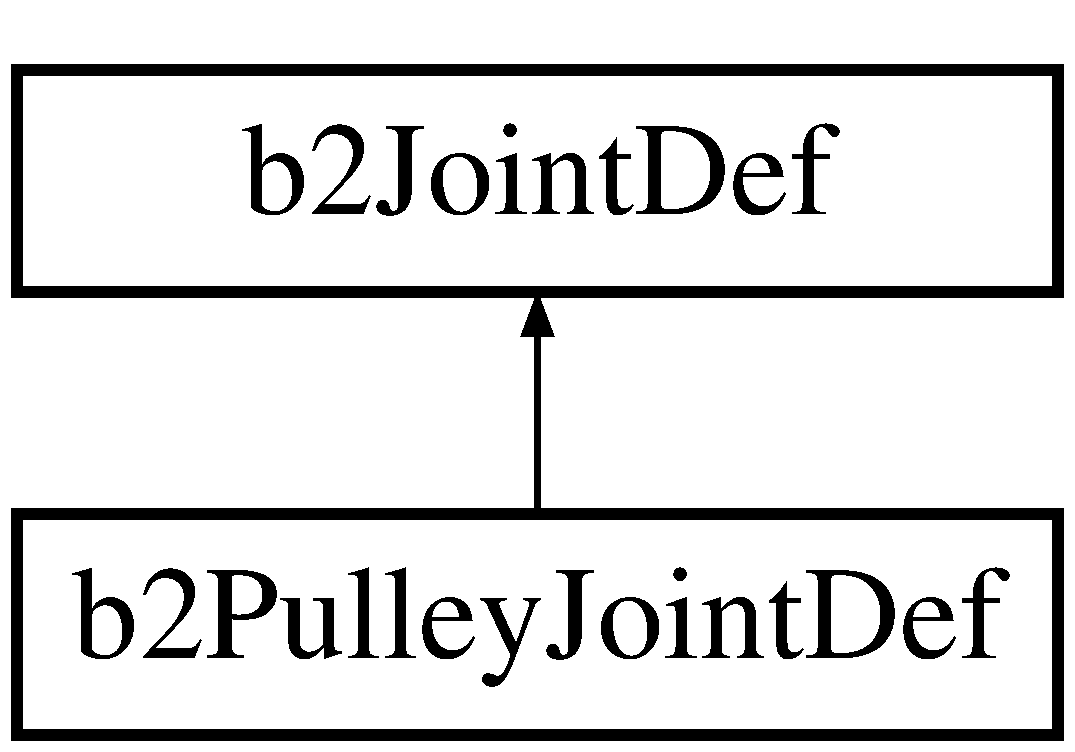
\includegraphics[height=2.000000cm]{structb2PulleyJointDef}
\end{center}
\end{figure}
\subsection*{Public Member Functions}
\begin{DoxyCompactItemize}
\item 
\mbox{\Hypertarget{structb2PulleyJointDef_abef614a93562b82aa3b5f8cac17d1ce8}\label{structb2PulleyJointDef_abef614a93562b82aa3b5f8cac17d1ce8}} 
void \mbox{\hyperlink{structb2PulleyJointDef_abef614a93562b82aa3b5f8cac17d1ce8}{Initialize}} (\mbox{\hyperlink{classb2Body}{b2\+Body}} $\ast$\mbox{\hyperlink{structb2JointDef_a8cd54c93da396be75a9788f2c6897f05}{bodyA}}, \mbox{\hyperlink{classb2Body}{b2\+Body}} $\ast$\mbox{\hyperlink{structb2JointDef_aa4f4dee2fbcd12187b19506b60e68e3d}{bodyB}}, const \mbox{\hyperlink{structb2Vec2}{b2\+Vec2}} \&\mbox{\hyperlink{structb2PulleyJointDef_aae77c020ce4629ab9e03560e28aa853d}{ground\+AnchorA}}, const \mbox{\hyperlink{structb2Vec2}{b2\+Vec2}} \&\mbox{\hyperlink{structb2PulleyJointDef_aa412b9f3bffd1fb69ace14f9b3e03b82}{ground\+AnchorB}}, const \mbox{\hyperlink{structb2Vec2}{b2\+Vec2}} \&anchorA, const \mbox{\hyperlink{structb2Vec2}{b2\+Vec2}} \&anchorB, float32 \mbox{\hyperlink{structb2PulleyJointDef_af35074246aeacbf239c11682642b31f5}{ratio}})
\begin{DoxyCompactList}\small\item\em Initialize the bodies, anchors, lengths, max lengths, and ratio using the world anchors. \end{DoxyCompactList}\end{DoxyCompactItemize}
\subsection*{Public Attributes}
\begin{DoxyCompactItemize}
\item 
\mbox{\Hypertarget{structb2PulleyJointDef_aae77c020ce4629ab9e03560e28aa853d}\label{structb2PulleyJointDef_aae77c020ce4629ab9e03560e28aa853d}} 
\mbox{\hyperlink{structb2Vec2}{b2\+Vec2}} \mbox{\hyperlink{structb2PulleyJointDef_aae77c020ce4629ab9e03560e28aa853d}{ground\+AnchorA}}
\begin{DoxyCompactList}\small\item\em The first ground anchor in world coordinates. This point never moves. \end{DoxyCompactList}\item 
\mbox{\Hypertarget{structb2PulleyJointDef_aa412b9f3bffd1fb69ace14f9b3e03b82}\label{structb2PulleyJointDef_aa412b9f3bffd1fb69ace14f9b3e03b82}} 
\mbox{\hyperlink{structb2Vec2}{b2\+Vec2}} \mbox{\hyperlink{structb2PulleyJointDef_aa412b9f3bffd1fb69ace14f9b3e03b82}{ground\+AnchorB}}
\begin{DoxyCompactList}\small\item\em The second ground anchor in world coordinates. This point never moves. \end{DoxyCompactList}\item 
\mbox{\Hypertarget{structb2PulleyJointDef_ad7677a4ad02a6e7cb8699fc5012eac3e}\label{structb2PulleyJointDef_ad7677a4ad02a6e7cb8699fc5012eac3e}} 
\mbox{\hyperlink{structb2Vec2}{b2\+Vec2}} \mbox{\hyperlink{structb2PulleyJointDef_ad7677a4ad02a6e7cb8699fc5012eac3e}{local\+AnchorA}}
\begin{DoxyCompactList}\small\item\em The local anchor point relative to bodyA\textquotesingle{}s origin. \end{DoxyCompactList}\item 
\mbox{\Hypertarget{structb2PulleyJointDef_aed3f9c9f5f4145ceb32e7e164de73144}\label{structb2PulleyJointDef_aed3f9c9f5f4145ceb32e7e164de73144}} 
\mbox{\hyperlink{structb2Vec2}{b2\+Vec2}} \mbox{\hyperlink{structb2PulleyJointDef_aed3f9c9f5f4145ceb32e7e164de73144}{local\+AnchorB}}
\begin{DoxyCompactList}\small\item\em The local anchor point relative to bodyB\textquotesingle{}s origin. \end{DoxyCompactList}\item 
\mbox{\Hypertarget{structb2PulleyJointDef_a51d945882c1d7a78af2b0e9ffb31a33b}\label{structb2PulleyJointDef_a51d945882c1d7a78af2b0e9ffb31a33b}} 
float32 \mbox{\hyperlink{structb2PulleyJointDef_a51d945882c1d7a78af2b0e9ffb31a33b}{lengthA}}
\begin{DoxyCompactList}\small\item\em The a reference length for the segment attached to bodyA. \end{DoxyCompactList}\item 
\mbox{\Hypertarget{structb2PulleyJointDef_a5857d5b5b9880b6c8201ce3ee8c3eef0}\label{structb2PulleyJointDef_a5857d5b5b9880b6c8201ce3ee8c3eef0}} 
float32 \mbox{\hyperlink{structb2PulleyJointDef_a5857d5b5b9880b6c8201ce3ee8c3eef0}{lengthB}}
\begin{DoxyCompactList}\small\item\em The a reference length for the segment attached to bodyB. \end{DoxyCompactList}\item 
\mbox{\Hypertarget{structb2PulleyJointDef_af35074246aeacbf239c11682642b31f5}\label{structb2PulleyJointDef_af35074246aeacbf239c11682642b31f5}} 
float32 \mbox{\hyperlink{structb2PulleyJointDef_af35074246aeacbf239c11682642b31f5}{ratio}}
\begin{DoxyCompactList}\small\item\em The pulley ratio, used to simulate a block-\/and-\/tackle. \end{DoxyCompactList}\end{DoxyCompactItemize}


\subsection{Detailed Description}
Pulley joint definition. This requires two ground anchors, two dynamic body anchor points, and a pulley ratio. 

The documentation for this struct was generated from the following files\+:\begin{DoxyCompactItemize}
\item 
Dynamics/\+Joints/b2\+Pulley\+Joint.\+h\item 
Dynamics/\+Joints/b2\+Pulley\+Joint.\+cpp\end{DoxyCompactItemize}

\hypertarget{classb2QueryCallback}{}\section{b2\+Query\+Callback Class Reference}
\label{classb2QueryCallback}\index{b2\+Query\+Callback@{b2\+Query\+Callback}}


{\ttfamily \#include $<$b2\+World\+Callbacks.\+h$>$}

\subsection*{Public Member Functions}
\begin{DoxyCompactItemize}
\item 
virtual bool \mbox{\hyperlink{classb2QueryCallback_a187dd04dd0f5164fb05c2ce2cbfd9ee5}{Report\+Fixture}} (\mbox{\hyperlink{classb2Fixture}{b2\+Fixture}} $\ast$fixture)=0
\end{DoxyCompactItemize}


\subsection{Detailed Description}
Callback class for A\+A\+BB queries. See b2\+World\+::\+Query 

\subsection{Member Function Documentation}
\mbox{\Hypertarget{classb2QueryCallback_a187dd04dd0f5164fb05c2ce2cbfd9ee5}\label{classb2QueryCallback_a187dd04dd0f5164fb05c2ce2cbfd9ee5}} 
\index{b2\+Query\+Callback@{b2\+Query\+Callback}!Report\+Fixture@{Report\+Fixture}}
\index{Report\+Fixture@{Report\+Fixture}!b2\+Query\+Callback@{b2\+Query\+Callback}}
\subsubsection{\texorpdfstring{Report\+Fixture()}{ReportFixture()}}
{\footnotesize\ttfamily virtual bool b2\+Query\+Callback\+::\+Report\+Fixture (\begin{DoxyParamCaption}\item[{\mbox{\hyperlink{classb2Fixture}{b2\+Fixture}} $\ast$}]{fixture }\end{DoxyParamCaption})\hspace{0.3cm}{\ttfamily [pure virtual]}}

Called for each fixture found in the query A\+A\+BB. \begin{DoxyReturn}{Returns}
false to terminate the query. 
\end{DoxyReturn}


The documentation for this class was generated from the following file\+:\begin{DoxyCompactItemize}
\item 
Dynamics/b2\+World\+Callbacks.\+h\end{DoxyCompactItemize}

\hypertarget{classb2RayCastCallback}{}\section{b2\+Ray\+Cast\+Callback Class Reference}
\label{classb2RayCastCallback}\index{b2\+Ray\+Cast\+Callback@{b2\+Ray\+Cast\+Callback}}


{\ttfamily \#include $<$b2\+World\+Callbacks.\+h$>$}

\subsection*{Public Member Functions}
\begin{DoxyCompactItemize}
\item 
virtual float32 \mbox{\hyperlink{classb2RayCastCallback_a658d5c8e89e0c73230cc8bddade4f3a4}{Report\+Fixture}} (\mbox{\hyperlink{classb2Fixture}{b2\+Fixture}} $\ast$fixture, const \mbox{\hyperlink{structb2Vec2}{b2\+Vec2}} \&point, const \mbox{\hyperlink{structb2Vec2}{b2\+Vec2}} \&normal, float32 fraction)=0
\end{DoxyCompactItemize}


\subsection{Detailed Description}
Callback class for ray casts. See \mbox{\hyperlink{classb2World_aa9955d94a254253997daaf16ce77bab6}{b2\+World\+::\+Ray\+Cast}} 

\subsection{Member Function Documentation}
\mbox{\Hypertarget{classb2RayCastCallback_a658d5c8e89e0c73230cc8bddade4f3a4}\label{classb2RayCastCallback_a658d5c8e89e0c73230cc8bddade4f3a4}} 
\index{b2\+Ray\+Cast\+Callback@{b2\+Ray\+Cast\+Callback}!Report\+Fixture@{Report\+Fixture}}
\index{Report\+Fixture@{Report\+Fixture}!b2\+Ray\+Cast\+Callback@{b2\+Ray\+Cast\+Callback}}
\subsubsection{\texorpdfstring{Report\+Fixture()}{ReportFixture()}}
{\footnotesize\ttfamily virtual float32 b2\+Ray\+Cast\+Callback\+::\+Report\+Fixture (\begin{DoxyParamCaption}\item[{\mbox{\hyperlink{classb2Fixture}{b2\+Fixture}} $\ast$}]{fixture,  }\item[{const \mbox{\hyperlink{structb2Vec2}{b2\+Vec2}} \&}]{point,  }\item[{const \mbox{\hyperlink{structb2Vec2}{b2\+Vec2}} \&}]{normal,  }\item[{float32}]{fraction }\end{DoxyParamCaption})\hspace{0.3cm}{\ttfamily [pure virtual]}}

Called for each fixture found in the query. You control how the ray cast proceeds by returning a float\+: return -\/1\+: ignore this fixture and continue return 0\+: terminate the ray cast return fraction\+: clip the ray to this point return 1\+: don\textquotesingle{}t clip the ray and continue 
\begin{DoxyParams}{Parameters}
{\em fixture} & the fixture hit by the ray \\
\hline
{\em point} & the point of initial intersection \\
\hline
{\em normal} & the normal vector at the point of intersection \\
\hline
\end{DoxyParams}
\begin{DoxyReturn}{Returns}
-\/1 to filter, 0 to terminate, fraction to clip the ray for closest hit, 1 to continue 
\end{DoxyReturn}


The documentation for this class was generated from the following file\+:\begin{DoxyCompactItemize}
\item 
Dynamics/b2\+World\+Callbacks.\+h\end{DoxyCompactItemize}

\hypertarget{structb2RayCastInput}{}\section{b2\+Ray\+Cast\+Input Struct Reference}
\label{structb2RayCastInput}\index{b2\+Ray\+Cast\+Input@{b2\+Ray\+Cast\+Input}}


Ray-\/cast input data. The ray extends from p1 to p1 + max\+Fraction $\ast$ (p2 -\/ p1).  




{\ttfamily \#include $<$b2\+Collision.\+h$>$}

\subsection*{Public Attributes}
\begin{DoxyCompactItemize}
\item 
\mbox{\Hypertarget{structb2RayCastInput_a7254a7062422833b1124fa464ab4caf3}\label{structb2RayCastInput_a7254a7062422833b1124fa464ab4caf3}} 
\mbox{\hyperlink{structb2Vec2}{b2\+Vec2}} {\bfseries p1}
\item 
\mbox{\Hypertarget{structb2RayCastInput_a850102c843469781a3a627c871043d0b}\label{structb2RayCastInput_a850102c843469781a3a627c871043d0b}} 
\mbox{\hyperlink{structb2Vec2}{b2\+Vec2}} {\bfseries p2}
\item 
\mbox{\Hypertarget{structb2RayCastInput_acb5c88e0ef2c3716a1334611522ab0b2}\label{structb2RayCastInput_acb5c88e0ef2c3716a1334611522ab0b2}} 
float32 {\bfseries max\+Fraction}
\end{DoxyCompactItemize}


\subsection{Detailed Description}
Ray-\/cast input data. The ray extends from p1 to p1 + max\+Fraction $\ast$ (p2 -\/ p1). 

The documentation for this struct was generated from the following file\+:\begin{DoxyCompactItemize}
\item 
Collision/\mbox{\hyperlink{b2Collision_8h}{b2\+Collision.\+h}}\end{DoxyCompactItemize}

\hypertarget{structb2RayCastOutput}{}\section{b2\+Ray\+Cast\+Output Struct Reference}
\label{structb2RayCastOutput}\index{b2\+Ray\+Cast\+Output@{b2\+Ray\+Cast\+Output}}


{\ttfamily \#include $<$b2\+Collision.\+h$>$}

\subsection*{Public Attributes}
\begin{DoxyCompactItemize}
\item 
\mbox{\Hypertarget{structb2RayCastOutput_aa9bbfe75afa23c21e85cb1bd3736529b}\label{structb2RayCastOutput_aa9bbfe75afa23c21e85cb1bd3736529b}} 
\mbox{\hyperlink{structb2Vec2}{b2\+Vec2}} {\bfseries normal}
\item 
\mbox{\Hypertarget{structb2RayCastOutput_a191c69bb399304bfe30c69e2158b3f29}\label{structb2RayCastOutput_a191c69bb399304bfe30c69e2158b3f29}} 
float32 {\bfseries fraction}
\end{DoxyCompactItemize}


\subsection{Detailed Description}
Ray-\/cast output data. The ray hits at p1 + fraction $\ast$ (p2 -\/ p1), where p1 and p2 come from \mbox{\hyperlink{structb2RayCastInput}{b2\+Ray\+Cast\+Input}}. 

The documentation for this struct was generated from the following file\+:\begin{DoxyCompactItemize}
\item 
Collision/\mbox{\hyperlink{b2Collision_8h}{b2\+Collision.\+h}}\end{DoxyCompactItemize}

\hypertarget{structb2ReferenceFace}{}\section{b2\+Reference\+Face Struct Reference}
\label{structb2ReferenceFace}\index{b2\+Reference\+Face@{b2\+Reference\+Face}}
\subsection*{Public Attributes}
\begin{DoxyCompactItemize}
\item 
\mbox{\Hypertarget{structb2ReferenceFace_a987d346858f5c1dd1de0dfddab779324}\label{structb2ReferenceFace_a987d346858f5c1dd1de0dfddab779324}} 
int32 {\bfseries i1}
\item 
\mbox{\Hypertarget{structb2ReferenceFace_a838ab3e4a81b71cfaa450eb214584353}\label{structb2ReferenceFace_a838ab3e4a81b71cfaa450eb214584353}} 
int32 {\bfseries i2}
\item 
\mbox{\Hypertarget{structb2ReferenceFace_a20165b58f2e81b78ed3a099ef85737ac}\label{structb2ReferenceFace_a20165b58f2e81b78ed3a099ef85737ac}} 
\mbox{\hyperlink{structb2Vec2}{b2\+Vec2}} {\bfseries v1}
\item 
\mbox{\Hypertarget{structb2ReferenceFace_aa89eb5b51e9ee680b97c33041658f9ab}\label{structb2ReferenceFace_aa89eb5b51e9ee680b97c33041658f9ab}} 
\mbox{\hyperlink{structb2Vec2}{b2\+Vec2}} {\bfseries v2}
\item 
\mbox{\Hypertarget{structb2ReferenceFace_a4ba73696920306d3c8fecc35a4433029}\label{structb2ReferenceFace_a4ba73696920306d3c8fecc35a4433029}} 
\mbox{\hyperlink{structb2Vec2}{b2\+Vec2}} {\bfseries normal}
\item 
\mbox{\Hypertarget{structb2ReferenceFace_a478026ee3fa0d8d1349b01928eb9e947}\label{structb2ReferenceFace_a478026ee3fa0d8d1349b01928eb9e947}} 
\mbox{\hyperlink{structb2Vec2}{b2\+Vec2}} {\bfseries side\+Normal1}
\item 
\mbox{\Hypertarget{structb2ReferenceFace_a7e2a902ed8f499fbb4305d51ce687876}\label{structb2ReferenceFace_a7e2a902ed8f499fbb4305d51ce687876}} 
float32 {\bfseries side\+Offset1}
\item 
\mbox{\Hypertarget{structb2ReferenceFace_ad272f9369fbc1d28f60f77defd757dbd}\label{structb2ReferenceFace_ad272f9369fbc1d28f60f77defd757dbd}} 
\mbox{\hyperlink{structb2Vec2}{b2\+Vec2}} {\bfseries side\+Normal2}
\item 
\mbox{\Hypertarget{structb2ReferenceFace_a7fa70d9f4bfc4cdf792408ffe204d017}\label{structb2ReferenceFace_a7fa70d9f4bfc4cdf792408ffe204d017}} 
float32 {\bfseries side\+Offset2}
\end{DoxyCompactItemize}


The documentation for this struct was generated from the following file\+:\begin{DoxyCompactItemize}
\item 
Collision/b2\+Collide\+Edge.\+cpp\end{DoxyCompactItemize}

\hypertarget{classb2RevoluteJoint}{}\section{b2\+Revolute\+Joint Class Reference}
\label{classb2RevoluteJoint}\index{b2\+Revolute\+Joint@{b2\+Revolute\+Joint}}


{\ttfamily \#include $<$b2\+Revolute\+Joint.\+h$>$}

Inheritance diagram for b2\+Revolute\+Joint\+:\begin{figure}[H]
\begin{center}
\leavevmode
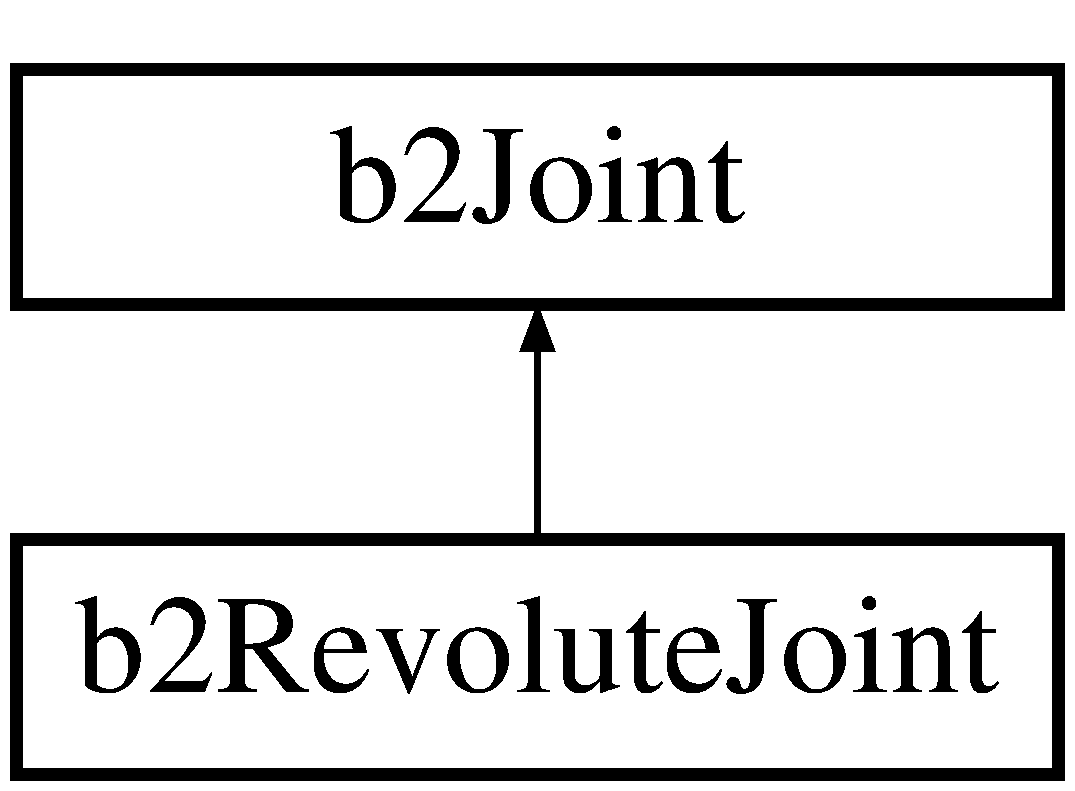
\includegraphics[height=2.000000cm]{classb2RevoluteJoint}
\end{center}
\end{figure}
\subsection*{Public Member Functions}
\begin{DoxyCompactItemize}
\item 
\mbox{\Hypertarget{classb2RevoluteJoint_a9878591c460a4e1575f8a77c237608ae}\label{classb2RevoluteJoint_a9878591c460a4e1575f8a77c237608ae}} 
\mbox{\hyperlink{structb2Vec2}{b2\+Vec2}} \mbox{\hyperlink{classb2RevoluteJoint_a9878591c460a4e1575f8a77c237608ae}{Get\+AnchorA}} () const override
\begin{DoxyCompactList}\small\item\em Get the anchor point on bodyA in world coordinates. \end{DoxyCompactList}\item 
\mbox{\Hypertarget{classb2RevoluteJoint_aa30a5d414b2ff699cc17567ff6e53e6b}\label{classb2RevoluteJoint_aa30a5d414b2ff699cc17567ff6e53e6b}} 
\mbox{\hyperlink{structb2Vec2}{b2\+Vec2}} \mbox{\hyperlink{classb2RevoluteJoint_aa30a5d414b2ff699cc17567ff6e53e6b}{Get\+AnchorB}} () const override
\begin{DoxyCompactList}\small\item\em Get the anchor point on bodyB in world coordinates. \end{DoxyCompactList}\item 
\mbox{\Hypertarget{classb2RevoluteJoint_af8cefd09d50a4e349613722809b8c823}\label{classb2RevoluteJoint_af8cefd09d50a4e349613722809b8c823}} 
const \mbox{\hyperlink{structb2Vec2}{b2\+Vec2}} \& \mbox{\hyperlink{classb2RevoluteJoint_af8cefd09d50a4e349613722809b8c823}{Get\+Local\+AnchorA}} () const
\begin{DoxyCompactList}\small\item\em The local anchor point relative to bodyA\textquotesingle{}s origin. \end{DoxyCompactList}\item 
\mbox{\Hypertarget{classb2RevoluteJoint_ac58e115df370181adc1ea1c486d84dc6}\label{classb2RevoluteJoint_ac58e115df370181adc1ea1c486d84dc6}} 
const \mbox{\hyperlink{structb2Vec2}{b2\+Vec2}} \& \mbox{\hyperlink{classb2RevoluteJoint_ac58e115df370181adc1ea1c486d84dc6}{Get\+Local\+AnchorB}} () const
\begin{DoxyCompactList}\small\item\em The local anchor point relative to bodyB\textquotesingle{}s origin. \end{DoxyCompactList}\item 
\mbox{\Hypertarget{classb2RevoluteJoint_ae84b9659fe94f41f54f43d3f64ee0741}\label{classb2RevoluteJoint_ae84b9659fe94f41f54f43d3f64ee0741}} 
float32 \mbox{\hyperlink{classb2RevoluteJoint_ae84b9659fe94f41f54f43d3f64ee0741}{Get\+Reference\+Angle}} () const
\begin{DoxyCompactList}\small\item\em Get the reference angle. \end{DoxyCompactList}\item 
\mbox{\Hypertarget{classb2RevoluteJoint_a2a83b2276c71bf287771004838f2b507}\label{classb2RevoluteJoint_a2a83b2276c71bf287771004838f2b507}} 
float32 \mbox{\hyperlink{classb2RevoluteJoint_a2a83b2276c71bf287771004838f2b507}{Get\+Joint\+Angle}} () const
\begin{DoxyCompactList}\small\item\em Get the current joint angle in radians. \end{DoxyCompactList}\item 
\mbox{\Hypertarget{classb2RevoluteJoint_a631b7bd2c72b61f03b6efc605308092f}\label{classb2RevoluteJoint_a631b7bd2c72b61f03b6efc605308092f}} 
float32 \mbox{\hyperlink{classb2RevoluteJoint_a631b7bd2c72b61f03b6efc605308092f}{Get\+Joint\+Speed}} () const
\begin{DoxyCompactList}\small\item\em Get the current joint angle speed in radians per second. \end{DoxyCompactList}\item 
\mbox{\Hypertarget{classb2RevoluteJoint_a84ff9c4f82b3e7d27a4390164f81f3ab}\label{classb2RevoluteJoint_a84ff9c4f82b3e7d27a4390164f81f3ab}} 
bool \mbox{\hyperlink{classb2RevoluteJoint_a84ff9c4f82b3e7d27a4390164f81f3ab}{Is\+Limit\+Enabled}} () const
\begin{DoxyCompactList}\small\item\em Is the joint limit enabled? \end{DoxyCompactList}\item 
\mbox{\Hypertarget{classb2RevoluteJoint_a56bdfdd04e906e52d0258f6a481b9093}\label{classb2RevoluteJoint_a56bdfdd04e906e52d0258f6a481b9093}} 
void \mbox{\hyperlink{classb2RevoluteJoint_a56bdfdd04e906e52d0258f6a481b9093}{Enable\+Limit}} (bool flag)
\begin{DoxyCompactList}\small\item\em Enable/disable the joint limit. \end{DoxyCompactList}\item 
\mbox{\Hypertarget{classb2RevoluteJoint_a1e34ad0cc3289d90bff8140c5d6261d2}\label{classb2RevoluteJoint_a1e34ad0cc3289d90bff8140c5d6261d2}} 
float32 \mbox{\hyperlink{classb2RevoluteJoint_a1e34ad0cc3289d90bff8140c5d6261d2}{Get\+Lower\+Limit}} () const
\begin{DoxyCompactList}\small\item\em Get the lower joint limit in radians. \end{DoxyCompactList}\item 
\mbox{\Hypertarget{classb2RevoluteJoint_a5c30cf83116841607d4d819985732efb}\label{classb2RevoluteJoint_a5c30cf83116841607d4d819985732efb}} 
float32 \mbox{\hyperlink{classb2RevoluteJoint_a5c30cf83116841607d4d819985732efb}{Get\+Upper\+Limit}} () const
\begin{DoxyCompactList}\small\item\em Get the upper joint limit in radians. \end{DoxyCompactList}\item 
\mbox{\Hypertarget{classb2RevoluteJoint_a32f9393d8a6b993fd523f0f643c28107}\label{classb2RevoluteJoint_a32f9393d8a6b993fd523f0f643c28107}} 
void \mbox{\hyperlink{classb2RevoluteJoint_a32f9393d8a6b993fd523f0f643c28107}{Set\+Limits}} (float32 lower, float32 upper)
\begin{DoxyCompactList}\small\item\em Set the joint limits in radians. \end{DoxyCompactList}\item 
\mbox{\Hypertarget{classb2RevoluteJoint_a37d5744e89991ebe01b974c4d15a21b5}\label{classb2RevoluteJoint_a37d5744e89991ebe01b974c4d15a21b5}} 
bool \mbox{\hyperlink{classb2RevoluteJoint_a37d5744e89991ebe01b974c4d15a21b5}{Is\+Motor\+Enabled}} () const
\begin{DoxyCompactList}\small\item\em Is the joint motor enabled? \end{DoxyCompactList}\item 
\mbox{\Hypertarget{classb2RevoluteJoint_a80ed5a07d9a0e07d010808a73ffae6ff}\label{classb2RevoluteJoint_a80ed5a07d9a0e07d010808a73ffae6ff}} 
void \mbox{\hyperlink{classb2RevoluteJoint_a80ed5a07d9a0e07d010808a73ffae6ff}{Enable\+Motor}} (bool flag)
\begin{DoxyCompactList}\small\item\em Enable/disable the joint motor. \end{DoxyCompactList}\item 
\mbox{\Hypertarget{classb2RevoluteJoint_a56f60bb1ea69048c8a455da49d62bf65}\label{classb2RevoluteJoint_a56f60bb1ea69048c8a455da49d62bf65}} 
void \mbox{\hyperlink{classb2RevoluteJoint_a56f60bb1ea69048c8a455da49d62bf65}{Set\+Motor\+Speed}} (float32 speed)
\begin{DoxyCompactList}\small\item\em Set the motor speed in radians per second. \end{DoxyCompactList}\item 
\mbox{\Hypertarget{classb2RevoluteJoint_abb1fa43d5779a1164ddfedf6130d7ff2}\label{classb2RevoluteJoint_abb1fa43d5779a1164ddfedf6130d7ff2}} 
float32 \mbox{\hyperlink{classb2RevoluteJoint_abb1fa43d5779a1164ddfedf6130d7ff2}{Get\+Motor\+Speed}} () const
\begin{DoxyCompactList}\small\item\em Get the motor speed in radians per second. \end{DoxyCompactList}\item 
\mbox{\Hypertarget{classb2RevoluteJoint_a41779d7ec05be33e6368ef00123a3581}\label{classb2RevoluteJoint_a41779d7ec05be33e6368ef00123a3581}} 
void \mbox{\hyperlink{classb2RevoluteJoint_a41779d7ec05be33e6368ef00123a3581}{Set\+Max\+Motor\+Torque}} (float32 torque)
\begin{DoxyCompactList}\small\item\em Set the maximum motor torque, usually in N-\/m. \end{DoxyCompactList}\item 
\mbox{\Hypertarget{classb2RevoluteJoint_a878308eb3e299e15ac9dc88d48671d51}\label{classb2RevoluteJoint_a878308eb3e299e15ac9dc88d48671d51}} 
float32 {\bfseries Get\+Max\+Motor\+Torque} () const
\item 
\mbox{\hyperlink{structb2Vec2}{b2\+Vec2}} \mbox{\hyperlink{classb2RevoluteJoint_abeb7bf941589aed0d7f330a578a62024}{Get\+Reaction\+Force}} (float32 inv\+\_\+dt) const override
\item 
float32 \mbox{\hyperlink{classb2RevoluteJoint_aab61a3f330aa93ae28f657e36bc3db51}{Get\+Reaction\+Torque}} (float32 inv\+\_\+dt) const override
\item 
float32 \mbox{\hyperlink{classb2RevoluteJoint_a5abafb4d0c1df642f73a5d9faf615e26}{Get\+Motor\+Torque}} (float32 inv\+\_\+dt) const
\item 
\mbox{\Hypertarget{classb2RevoluteJoint_a408badabe21b169412a5c4a2f36bbbd8}\label{classb2RevoluteJoint_a408badabe21b169412a5c4a2f36bbbd8}} 
void \mbox{\hyperlink{classb2RevoluteJoint_a408badabe21b169412a5c4a2f36bbbd8}{Dump}} () override
\begin{DoxyCompactList}\small\item\em Dump to b2\+Log. \end{DoxyCompactList}\end{DoxyCompactItemize}
\subsection*{Protected Member Functions}
\begin{DoxyCompactItemize}
\item 
\mbox{\Hypertarget{classb2RevoluteJoint_a2571c1438e909fb3518de6f88bb29e01}\label{classb2RevoluteJoint_a2571c1438e909fb3518de6f88bb29e01}} 
{\bfseries b2\+Revolute\+Joint} (const \mbox{\hyperlink{structb2RevoluteJointDef}{b2\+Revolute\+Joint\+Def}} $\ast$def)
\item 
\mbox{\Hypertarget{classb2RevoluteJoint_a5ddddb865cc297c66721ae443bfb40a4}\label{classb2RevoluteJoint_a5ddddb865cc297c66721ae443bfb40a4}} 
void {\bfseries Init\+Velocity\+Constraints} (const \mbox{\hyperlink{structb2SolverData}{b2\+Solver\+Data}} \&data) override
\item 
\mbox{\Hypertarget{classb2RevoluteJoint_a8eee8e87c79588ff041f1382b7fcbcd4}\label{classb2RevoluteJoint_a8eee8e87c79588ff041f1382b7fcbcd4}} 
void {\bfseries Solve\+Velocity\+Constraints} (const \mbox{\hyperlink{structb2SolverData}{b2\+Solver\+Data}} \&data) override
\item 
\mbox{\Hypertarget{classb2RevoluteJoint_a01cab9d9609926a6debcd457bb8068f2}\label{classb2RevoluteJoint_a01cab9d9609926a6debcd457bb8068f2}} 
bool {\bfseries Solve\+Position\+Constraints} (const \mbox{\hyperlink{structb2SolverData}{b2\+Solver\+Data}} \&data) override
\end{DoxyCompactItemize}
\subsection*{Protected Attributes}
\begin{DoxyCompactItemize}
\item 
\mbox{\Hypertarget{classb2RevoluteJoint_ad4ce801fa7bdd408b41310793e6b37f8}\label{classb2RevoluteJoint_ad4ce801fa7bdd408b41310793e6b37f8}} 
\mbox{\hyperlink{structb2Vec2}{b2\+Vec2}} {\bfseries m\+\_\+local\+AnchorA}
\item 
\mbox{\Hypertarget{classb2RevoluteJoint_ae206b6bcc7b6527d7d18f239d20a7ae9}\label{classb2RevoluteJoint_ae206b6bcc7b6527d7d18f239d20a7ae9}} 
\mbox{\hyperlink{structb2Vec2}{b2\+Vec2}} {\bfseries m\+\_\+local\+AnchorB}
\item 
\mbox{\Hypertarget{classb2RevoluteJoint_a00d576701b8e2ee886e9a59811b4df65}\label{classb2RevoluteJoint_a00d576701b8e2ee886e9a59811b4df65}} 
\mbox{\hyperlink{structb2Vec3}{b2\+Vec3}} {\bfseries m\+\_\+impulse}
\item 
\mbox{\Hypertarget{classb2RevoluteJoint_a9275ac791803aa38c225d06b05ecfc26}\label{classb2RevoluteJoint_a9275ac791803aa38c225d06b05ecfc26}} 
float32 {\bfseries m\+\_\+motor\+Impulse}
\item 
\mbox{\Hypertarget{classb2RevoluteJoint_a8fcdcbfc9fd51e8b5dc98ed8ea652e13}\label{classb2RevoluteJoint_a8fcdcbfc9fd51e8b5dc98ed8ea652e13}} 
bool {\bfseries m\+\_\+enable\+Motor}
\item 
\mbox{\Hypertarget{classb2RevoluteJoint_a06ab30be0a455599bd3b5b6a11d6a43a}\label{classb2RevoluteJoint_a06ab30be0a455599bd3b5b6a11d6a43a}} 
float32 {\bfseries m\+\_\+max\+Motor\+Torque}
\item 
\mbox{\Hypertarget{classb2RevoluteJoint_a7b6f51d7aa4b0132b12ec1091fdebfca}\label{classb2RevoluteJoint_a7b6f51d7aa4b0132b12ec1091fdebfca}} 
float32 {\bfseries m\+\_\+motor\+Speed}
\item 
\mbox{\Hypertarget{classb2RevoluteJoint_adb179e134ac49c612201caa20340e090}\label{classb2RevoluteJoint_adb179e134ac49c612201caa20340e090}} 
bool {\bfseries m\+\_\+enable\+Limit}
\item 
\mbox{\Hypertarget{classb2RevoluteJoint_a7648b770a9165ee9cd97edcf2df6ed9e}\label{classb2RevoluteJoint_a7648b770a9165ee9cd97edcf2df6ed9e}} 
float32 {\bfseries m\+\_\+reference\+Angle}
\item 
\mbox{\Hypertarget{classb2RevoluteJoint_a7c57732200aae93368481970731630b1}\label{classb2RevoluteJoint_a7c57732200aae93368481970731630b1}} 
float32 {\bfseries m\+\_\+lower\+Angle}
\item 
\mbox{\Hypertarget{classb2RevoluteJoint_adf7a2ab69e1e7a72697a2c9d92877c52}\label{classb2RevoluteJoint_adf7a2ab69e1e7a72697a2c9d92877c52}} 
float32 {\bfseries m\+\_\+upper\+Angle}
\item 
\mbox{\Hypertarget{classb2RevoluteJoint_a2bdab138718ea7ccab67a37d0499286d}\label{classb2RevoluteJoint_a2bdab138718ea7ccab67a37d0499286d}} 
int32 {\bfseries m\+\_\+indexA}
\item 
\mbox{\Hypertarget{classb2RevoluteJoint_acbf266a053a6f3071bfdd53e0e6b3df8}\label{classb2RevoluteJoint_acbf266a053a6f3071bfdd53e0e6b3df8}} 
int32 {\bfseries m\+\_\+indexB}
\item 
\mbox{\Hypertarget{classb2RevoluteJoint_a6e33bbf932ce95efe072326199fa30f3}\label{classb2RevoluteJoint_a6e33bbf932ce95efe072326199fa30f3}} 
\mbox{\hyperlink{structb2Vec2}{b2\+Vec2}} {\bfseries m\+\_\+rA}
\item 
\mbox{\Hypertarget{classb2RevoluteJoint_afd72e453f92aa3214701a201c8f9dfe9}\label{classb2RevoluteJoint_afd72e453f92aa3214701a201c8f9dfe9}} 
\mbox{\hyperlink{structb2Vec2}{b2\+Vec2}} {\bfseries m\+\_\+rB}
\item 
\mbox{\Hypertarget{classb2RevoluteJoint_a70e2a385d097053453b4099094eb1154}\label{classb2RevoluteJoint_a70e2a385d097053453b4099094eb1154}} 
\mbox{\hyperlink{structb2Vec2}{b2\+Vec2}} {\bfseries m\+\_\+local\+CenterA}
\item 
\mbox{\Hypertarget{classb2RevoluteJoint_a322ec1f7c33a358db73b53ec58e3356b}\label{classb2RevoluteJoint_a322ec1f7c33a358db73b53ec58e3356b}} 
\mbox{\hyperlink{structb2Vec2}{b2\+Vec2}} {\bfseries m\+\_\+local\+CenterB}
\item 
\mbox{\Hypertarget{classb2RevoluteJoint_a28cd428903a7c62914d3473a40857fd2}\label{classb2RevoluteJoint_a28cd428903a7c62914d3473a40857fd2}} 
float32 {\bfseries m\+\_\+inv\+MassA}
\item 
\mbox{\Hypertarget{classb2RevoluteJoint_a4fd153ad1fcb65084455f9884fa8b9d7}\label{classb2RevoluteJoint_a4fd153ad1fcb65084455f9884fa8b9d7}} 
float32 {\bfseries m\+\_\+inv\+MassB}
\item 
\mbox{\Hypertarget{classb2RevoluteJoint_a948a49144e282f7db22b1f20379c6099}\label{classb2RevoluteJoint_a948a49144e282f7db22b1f20379c6099}} 
float32 {\bfseries m\+\_\+inv\+IA}
\item 
\mbox{\Hypertarget{classb2RevoluteJoint_a7c224fc59adebaa00590217ab8a2c685}\label{classb2RevoluteJoint_a7c224fc59adebaa00590217ab8a2c685}} 
float32 {\bfseries m\+\_\+inv\+IB}
\item 
\mbox{\Hypertarget{classb2RevoluteJoint_a284ae761074305d5032a2b666efb0650}\label{classb2RevoluteJoint_a284ae761074305d5032a2b666efb0650}} 
\mbox{\hyperlink{structb2Mat33}{b2\+Mat33}} {\bfseries m\+\_\+mass}
\item 
\mbox{\Hypertarget{classb2RevoluteJoint_aced7e455dd33ccb17a1d4ff9bb80c442}\label{classb2RevoluteJoint_aced7e455dd33ccb17a1d4ff9bb80c442}} 
float32 {\bfseries m\+\_\+motor\+Mass}
\item 
\mbox{\Hypertarget{classb2RevoluteJoint_abe77594f4773d21dabd8912d6630dc6a}\label{classb2RevoluteJoint_abe77594f4773d21dabd8912d6630dc6a}} 
b2\+Limit\+State {\bfseries m\+\_\+limit\+State}
\end{DoxyCompactItemize}
\subsection*{Friends}
\begin{DoxyCompactItemize}
\item 
\mbox{\Hypertarget{classb2RevoluteJoint_a54ade8ed3d794298108d7f4c4e4793fa}\label{classb2RevoluteJoint_a54ade8ed3d794298108d7f4c4e4793fa}} 
class {\bfseries b2\+Joint}
\item 
\mbox{\Hypertarget{classb2RevoluteJoint_a13c275221e30bb485e17e4e04553cb71}\label{classb2RevoluteJoint_a13c275221e30bb485e17e4e04553cb71}} 
class {\bfseries b2\+Gear\+Joint}
\end{DoxyCompactItemize}
\subsection*{Additional Inherited Members}


\subsection{Detailed Description}
A revolute joint constrains two bodies to share a common point while they are free to rotate about the point. The relative rotation about the shared point is the joint angle. You can limit the relative rotation with a joint limit that specifies a lower and upper angle. You can use a motor to drive the relative rotation about the shared point. A maximum motor torque is provided so that infinite forces are not generated. 

\subsection{Member Function Documentation}
\mbox{\Hypertarget{classb2RevoluteJoint_a5abafb4d0c1df642f73a5d9faf615e26}\label{classb2RevoluteJoint_a5abafb4d0c1df642f73a5d9faf615e26}} 
\index{b2\+Revolute\+Joint@{b2\+Revolute\+Joint}!Get\+Motor\+Torque@{Get\+Motor\+Torque}}
\index{Get\+Motor\+Torque@{Get\+Motor\+Torque}!b2\+Revolute\+Joint@{b2\+Revolute\+Joint}}
\subsubsection{\texorpdfstring{Get\+Motor\+Torque()}{GetMotorTorque()}}
{\footnotesize\ttfamily float32 b2\+Revolute\+Joint\+::\+Get\+Motor\+Torque (\begin{DoxyParamCaption}\item[{float32}]{inv\+\_\+dt }\end{DoxyParamCaption}) const}

Get the current motor torque given the inverse time step. Unit is N$\ast$m. \mbox{\Hypertarget{classb2RevoluteJoint_abeb7bf941589aed0d7f330a578a62024}\label{classb2RevoluteJoint_abeb7bf941589aed0d7f330a578a62024}} 
\index{b2\+Revolute\+Joint@{b2\+Revolute\+Joint}!Get\+Reaction\+Force@{Get\+Reaction\+Force}}
\index{Get\+Reaction\+Force@{Get\+Reaction\+Force}!b2\+Revolute\+Joint@{b2\+Revolute\+Joint}}
\subsubsection{\texorpdfstring{Get\+Reaction\+Force()}{GetReactionForce()}}
{\footnotesize\ttfamily \mbox{\hyperlink{structb2Vec2}{b2\+Vec2}} b2\+Revolute\+Joint\+::\+Get\+Reaction\+Force (\begin{DoxyParamCaption}\item[{float32}]{inv\+\_\+dt }\end{DoxyParamCaption}) const\hspace{0.3cm}{\ttfamily [override]}, {\ttfamily [virtual]}}

Get the reaction force given the inverse time step. Unit is N. 

Implements \mbox{\hyperlink{classb2Joint_a7e0eddefb9b69ad050b8ef6425838a74}{b2\+Joint}}.

\mbox{\Hypertarget{classb2RevoluteJoint_aab61a3f330aa93ae28f657e36bc3db51}\label{classb2RevoluteJoint_aab61a3f330aa93ae28f657e36bc3db51}} 
\index{b2\+Revolute\+Joint@{b2\+Revolute\+Joint}!Get\+Reaction\+Torque@{Get\+Reaction\+Torque}}
\index{Get\+Reaction\+Torque@{Get\+Reaction\+Torque}!b2\+Revolute\+Joint@{b2\+Revolute\+Joint}}
\subsubsection{\texorpdfstring{Get\+Reaction\+Torque()}{GetReactionTorque()}}
{\footnotesize\ttfamily float32 b2\+Revolute\+Joint\+::\+Get\+Reaction\+Torque (\begin{DoxyParamCaption}\item[{float32}]{inv\+\_\+dt }\end{DoxyParamCaption}) const\hspace{0.3cm}{\ttfamily [override]}, {\ttfamily [virtual]}}

Get the reaction torque due to the joint limit given the inverse time step. Unit is N$\ast$m. 

Implements \mbox{\hyperlink{classb2Joint_ae355e441c2aa842777dc04e24f15ced0}{b2\+Joint}}.



The documentation for this class was generated from the following files\+:\begin{DoxyCompactItemize}
\item 
Dynamics/\+Joints/b2\+Revolute\+Joint.\+h\item 
Dynamics/\+Joints/b2\+Revolute\+Joint.\+cpp\end{DoxyCompactItemize}

\hypertarget{structb2RevoluteJointDef}{}\section{b2\+Revolute\+Joint\+Def Struct Reference}
\label{structb2RevoluteJointDef}\index{b2\+Revolute\+Joint\+Def@{b2\+Revolute\+Joint\+Def}}


{\ttfamily \#include $<$b2\+Revolute\+Joint.\+h$>$}

Inheritance diagram for b2\+Revolute\+Joint\+Def\+:\begin{figure}[H]
\begin{center}
\leavevmode
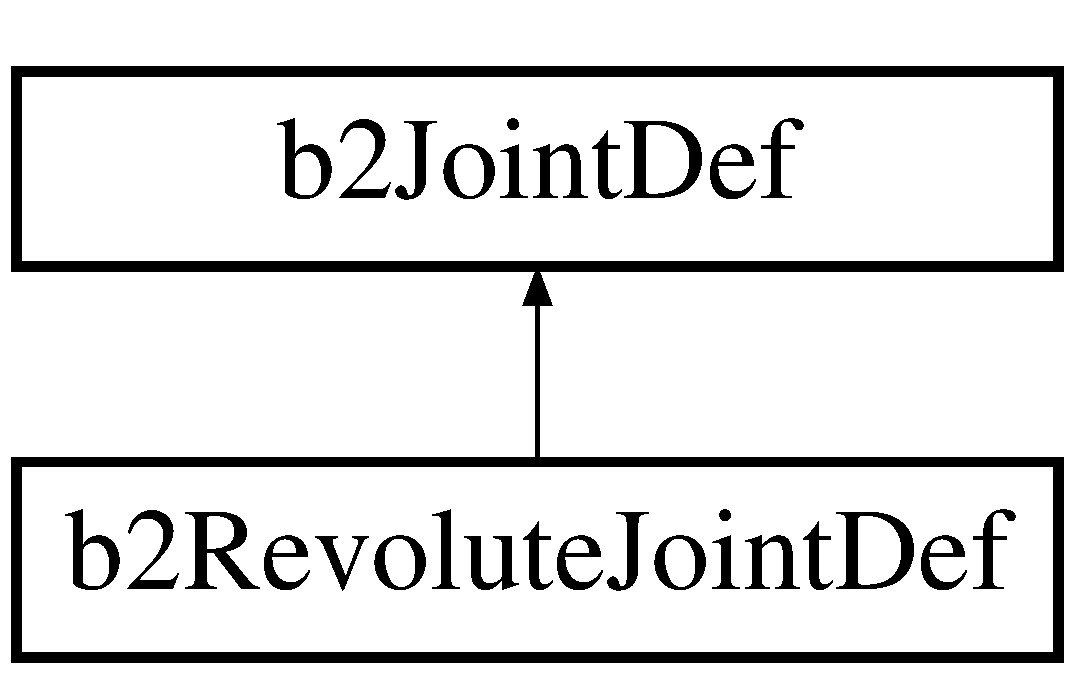
\includegraphics[height=2.000000cm]{structb2RevoluteJointDef}
\end{center}
\end{figure}
\subsection*{Public Member Functions}
\begin{DoxyCompactItemize}
\item 
void \mbox{\hyperlink{structb2RevoluteJointDef_a6401b2a663533415d032a525e4fa2806}{Initialize}} (\mbox{\hyperlink{classb2Body}{b2\+Body}} $\ast$\mbox{\hyperlink{structb2JointDef_a8cd54c93da396be75a9788f2c6897f05}{bodyA}}, \mbox{\hyperlink{classb2Body}{b2\+Body}} $\ast$\mbox{\hyperlink{structb2JointDef_aa4f4dee2fbcd12187b19506b60e68e3d}{bodyB}}, const \mbox{\hyperlink{structb2Vec2}{b2\+Vec2}} \&anchor)
\end{DoxyCompactItemize}
\subsection*{Public Attributes}
\begin{DoxyCompactItemize}
\item 
\mbox{\Hypertarget{structb2RevoluteJointDef_a76337d07aa63232a7b20d50decc862ae}\label{structb2RevoluteJointDef_a76337d07aa63232a7b20d50decc862ae}} 
\mbox{\hyperlink{structb2Vec2}{b2\+Vec2}} \mbox{\hyperlink{structb2RevoluteJointDef_a76337d07aa63232a7b20d50decc862ae}{local\+AnchorA}}
\begin{DoxyCompactList}\small\item\em The local anchor point relative to bodyA\textquotesingle{}s origin. \end{DoxyCompactList}\item 
\mbox{\Hypertarget{structb2RevoluteJointDef_a3f33bc1d9f6c22043a5ff2f1d89f04e0}\label{structb2RevoluteJointDef_a3f33bc1d9f6c22043a5ff2f1d89f04e0}} 
\mbox{\hyperlink{structb2Vec2}{b2\+Vec2}} \mbox{\hyperlink{structb2RevoluteJointDef_a3f33bc1d9f6c22043a5ff2f1d89f04e0}{local\+AnchorB}}
\begin{DoxyCompactList}\small\item\em The local anchor point relative to bodyB\textquotesingle{}s origin. \end{DoxyCompactList}\item 
\mbox{\Hypertarget{structb2RevoluteJointDef_a1858d897d5fea04c5e606a1ff73f64f8}\label{structb2RevoluteJointDef_a1858d897d5fea04c5e606a1ff73f64f8}} 
float32 \mbox{\hyperlink{structb2RevoluteJointDef_a1858d897d5fea04c5e606a1ff73f64f8}{reference\+Angle}}
\begin{DoxyCompactList}\small\item\em The bodyB angle minus bodyA angle in the reference state (radians). \end{DoxyCompactList}\item 
\mbox{\Hypertarget{structb2RevoluteJointDef_a2eaefc5fc5caf879cfd59ebcd852b756}\label{structb2RevoluteJointDef_a2eaefc5fc5caf879cfd59ebcd852b756}} 
bool \mbox{\hyperlink{structb2RevoluteJointDef_a2eaefc5fc5caf879cfd59ebcd852b756}{enable\+Limit}}
\begin{DoxyCompactList}\small\item\em A flag to enable joint limits. \end{DoxyCompactList}\item 
\mbox{\Hypertarget{structb2RevoluteJointDef_a24d0b2638a01405c77bd1c0de3e53de8}\label{structb2RevoluteJointDef_a24d0b2638a01405c77bd1c0de3e53de8}} 
float32 \mbox{\hyperlink{structb2RevoluteJointDef_a24d0b2638a01405c77bd1c0de3e53de8}{lower\+Angle}}
\begin{DoxyCompactList}\small\item\em The lower angle for the joint limit (radians). \end{DoxyCompactList}\item 
\mbox{\Hypertarget{structb2RevoluteJointDef_a692cfe333ad12afd5753a6ec54e39a66}\label{structb2RevoluteJointDef_a692cfe333ad12afd5753a6ec54e39a66}} 
float32 \mbox{\hyperlink{structb2RevoluteJointDef_a692cfe333ad12afd5753a6ec54e39a66}{upper\+Angle}}
\begin{DoxyCompactList}\small\item\em The upper angle for the joint limit (radians). \end{DoxyCompactList}\item 
\mbox{\Hypertarget{structb2RevoluteJointDef_aa94d9e66be9f03818d0cfbd9c70b2996}\label{structb2RevoluteJointDef_aa94d9e66be9f03818d0cfbd9c70b2996}} 
bool \mbox{\hyperlink{structb2RevoluteJointDef_aa94d9e66be9f03818d0cfbd9c70b2996}{enable\+Motor}}
\begin{DoxyCompactList}\small\item\em A flag to enable the joint motor. \end{DoxyCompactList}\item 
\mbox{\Hypertarget{structb2RevoluteJointDef_aced7cf768f4dcc3561576a39c7b92ec4}\label{structb2RevoluteJointDef_aced7cf768f4dcc3561576a39c7b92ec4}} 
float32 \mbox{\hyperlink{structb2RevoluteJointDef_aced7cf768f4dcc3561576a39c7b92ec4}{motor\+Speed}}
\begin{DoxyCompactList}\small\item\em The desired motor speed. Usually in radians per second. \end{DoxyCompactList}\item 
float32 \mbox{\hyperlink{structb2RevoluteJointDef_a9fc1b67fe6d1bc31f88cc2cfd681fe30}{max\+Motor\+Torque}}
\end{DoxyCompactItemize}


\subsection{Detailed Description}
Revolute joint definition. This requires defining an anchor point where the bodies are joined. The definition uses local anchor points so that the initial configuration can violate the constraint slightly. You also need to specify the initial relative angle for joint limits. This helps when saving and loading a game. The local anchor points are measured from the body\textquotesingle{}s origin rather than the center of mass because\+:
\begin{DoxyEnumerate}
\item you might not know where the center of mass will be.
\item if you add/remove shapes from a body and recompute the mass, the joints will be broken. 
\end{DoxyEnumerate}

\subsection{Member Function Documentation}
\mbox{\Hypertarget{structb2RevoluteJointDef_a6401b2a663533415d032a525e4fa2806}\label{structb2RevoluteJointDef_a6401b2a663533415d032a525e4fa2806}} 
\index{b2\+Revolute\+Joint\+Def@{b2\+Revolute\+Joint\+Def}!Initialize@{Initialize}}
\index{Initialize@{Initialize}!b2\+Revolute\+Joint\+Def@{b2\+Revolute\+Joint\+Def}}
\subsubsection{\texorpdfstring{Initialize()}{Initialize()}}
{\footnotesize\ttfamily void b2\+Revolute\+Joint\+Def\+::\+Initialize (\begin{DoxyParamCaption}\item[{\mbox{\hyperlink{classb2Body}{b2\+Body}} $\ast$}]{bodyA,  }\item[{\mbox{\hyperlink{classb2Body}{b2\+Body}} $\ast$}]{bodyB,  }\item[{const \mbox{\hyperlink{structb2Vec2}{b2\+Vec2}} \&}]{anchor }\end{DoxyParamCaption})}

Initialize the bodies, anchors, and reference angle using a world anchor point. 

\subsection{Member Data Documentation}
\mbox{\Hypertarget{structb2RevoluteJointDef_a9fc1b67fe6d1bc31f88cc2cfd681fe30}\label{structb2RevoluteJointDef_a9fc1b67fe6d1bc31f88cc2cfd681fe30}} 
\index{b2\+Revolute\+Joint\+Def@{b2\+Revolute\+Joint\+Def}!max\+Motor\+Torque@{max\+Motor\+Torque}}
\index{max\+Motor\+Torque@{max\+Motor\+Torque}!b2\+Revolute\+Joint\+Def@{b2\+Revolute\+Joint\+Def}}
\subsubsection{\texorpdfstring{max\+Motor\+Torque}{maxMotorTorque}}
{\footnotesize\ttfamily float32 b2\+Revolute\+Joint\+Def\+::max\+Motor\+Torque}

The maximum motor torque used to achieve the desired motor speed. Usually in N-\/m. 

The documentation for this struct was generated from the following files\+:\begin{DoxyCompactItemize}
\item 
Dynamics/\+Joints/b2\+Revolute\+Joint.\+h\item 
Dynamics/\+Joints/b2\+Revolute\+Joint.\+cpp\end{DoxyCompactItemize}

\hypertarget{classb2Rope}{}\section{b2\+Rope Class Reference}
\label{classb2Rope}\index{b2\+Rope@{b2\+Rope}}
\subsection*{Public Member Functions}
\begin{DoxyCompactItemize}
\item 
\mbox{\Hypertarget{classb2Rope_a2a672ca3310790f4af1beb123e597d70}\label{classb2Rope_a2a672ca3310790f4af1beb123e597d70}} 
void {\bfseries Initialize} (const \mbox{\hyperlink{structb2RopeDef}{b2\+Rope\+Def}} $\ast$def)
\item 
\mbox{\Hypertarget{classb2Rope_abe9ce398cef717b136645cbc37f38d70}\label{classb2Rope_abe9ce398cef717b136645cbc37f38d70}} 
void {\bfseries Step} (float32 time\+Step, int32 iterations)
\item 
\mbox{\Hypertarget{classb2Rope_afdf6f7234dbf73fa83a058452e3d492a}\label{classb2Rope_afdf6f7234dbf73fa83a058452e3d492a}} 
int32 {\bfseries Get\+Vertex\+Count} () const
\item 
\mbox{\Hypertarget{classb2Rope_acf2b433c741b90b3668ff4477b4a8319}\label{classb2Rope_acf2b433c741b90b3668ff4477b4a8319}} 
const \mbox{\hyperlink{structb2Vec2}{b2\+Vec2}} $\ast$ {\bfseries Get\+Vertices} () const
\item 
\mbox{\Hypertarget{classb2Rope_a9545f16b4ed203890a290d58ba56255c}\label{classb2Rope_a9545f16b4ed203890a290d58ba56255c}} 
void {\bfseries Draw} (\mbox{\hyperlink{classb2Draw}{b2\+Draw}} $\ast$draw) const
\item 
\mbox{\Hypertarget{classb2Rope_a8a1717a5e0b2c54d56fe438c8cae43b7}\label{classb2Rope_a8a1717a5e0b2c54d56fe438c8cae43b7}} 
void {\bfseries Set\+Angle} (float32 angle)
\end{DoxyCompactItemize}
\subsection*{Private Member Functions}
\begin{DoxyCompactItemize}
\item 
\mbox{\Hypertarget{classb2Rope_abb803e414e406151c8c22ef814519b2a}\label{classb2Rope_abb803e414e406151c8c22ef814519b2a}} 
void {\bfseries Solve\+C2} ()
\item 
\mbox{\Hypertarget{classb2Rope_ae18c19e30583e72e90ffb01674ba01ad}\label{classb2Rope_ae18c19e30583e72e90ffb01674ba01ad}} 
void {\bfseries Solve\+C3} ()
\end{DoxyCompactItemize}
\subsection*{Private Attributes}
\begin{DoxyCompactItemize}
\item 
\mbox{\Hypertarget{classb2Rope_a25cf0ed66027fcd262714cc95589a62f}\label{classb2Rope_a25cf0ed66027fcd262714cc95589a62f}} 
int32 {\bfseries m\+\_\+count}
\item 
\mbox{\Hypertarget{classb2Rope_ac86bcba951cc7e5db5504e4c9af1f0a4}\label{classb2Rope_ac86bcba951cc7e5db5504e4c9af1f0a4}} 
\mbox{\hyperlink{structb2Vec2}{b2\+Vec2}} $\ast$ {\bfseries m\+\_\+ps}
\item 
\mbox{\Hypertarget{classb2Rope_a3658cb1686cb50494e50dfc38ed43290}\label{classb2Rope_a3658cb1686cb50494e50dfc38ed43290}} 
\mbox{\hyperlink{structb2Vec2}{b2\+Vec2}} $\ast$ {\bfseries m\+\_\+p0s}
\item 
\mbox{\Hypertarget{classb2Rope_a228257fb879daf4e5b73d2c279a37c58}\label{classb2Rope_a228257fb879daf4e5b73d2c279a37c58}} 
\mbox{\hyperlink{structb2Vec2}{b2\+Vec2}} $\ast$ {\bfseries m\+\_\+vs}
\item 
\mbox{\Hypertarget{classb2Rope_a1854a191ae97904ba8182ba45b362d4d}\label{classb2Rope_a1854a191ae97904ba8182ba45b362d4d}} 
float32 $\ast$ {\bfseries m\+\_\+ims}
\item 
\mbox{\Hypertarget{classb2Rope_a73204bb0635c44c437c6724fb2a28b6d}\label{classb2Rope_a73204bb0635c44c437c6724fb2a28b6d}} 
float32 $\ast$ {\bfseries m\+\_\+\+Ls}
\item 
\mbox{\Hypertarget{classb2Rope_a777771aa70d1b0717b1df3e0cae161de}\label{classb2Rope_a777771aa70d1b0717b1df3e0cae161de}} 
float32 $\ast$ {\bfseries m\+\_\+as}
\item 
\mbox{\Hypertarget{classb2Rope_a982d2a7545454b62ab0a2b5eeb33b48c}\label{classb2Rope_a982d2a7545454b62ab0a2b5eeb33b48c}} 
\mbox{\hyperlink{structb2Vec2}{b2\+Vec2}} {\bfseries m\+\_\+gravity}
\item 
\mbox{\Hypertarget{classb2Rope_ac5bf18e49983f50ac6fbd3acbe954ccd}\label{classb2Rope_ac5bf18e49983f50ac6fbd3acbe954ccd}} 
float32 {\bfseries m\+\_\+damping}
\item 
\mbox{\Hypertarget{classb2Rope_ab37ff9d1d0485be2d670b090c067ab81}\label{classb2Rope_ab37ff9d1d0485be2d670b090c067ab81}} 
float32 {\bfseries m\+\_\+k2}
\item 
\mbox{\Hypertarget{classb2Rope_a7226de25915cfa1b7d216b46f30e2d22}\label{classb2Rope_a7226de25915cfa1b7d216b46f30e2d22}} 
float32 {\bfseries m\+\_\+k3}
\end{DoxyCompactItemize}


The documentation for this class was generated from the following files\+:\begin{DoxyCompactItemize}
\item 
Rope/b2\+Rope.\+h\item 
Rope/b2\+Rope.\+cpp\end{DoxyCompactItemize}

\hypertarget{structb2RopeDef}{}\section{b2\+Rope\+Def Struct Reference}
\label{structb2RopeDef}\index{b2\+Rope\+Def@{b2\+Rope\+Def}}
\subsection*{Public Attributes}
\begin{DoxyCompactItemize}
\item 
\mbox{\Hypertarget{structb2RopeDef_ae18ad98b9796c505ae62ce58fa2f7051}\label{structb2RopeDef_ae18ad98b9796c505ae62ce58fa2f7051}} 
\mbox{\hyperlink{structb2Vec2}{b2\+Vec2}} $\ast$ {\bfseries vertices}
\item 
\mbox{\Hypertarget{structb2RopeDef_a0c75d4289a807e31f32dc43a2276671f}\label{structb2RopeDef_a0c75d4289a807e31f32dc43a2276671f}} 
int32 {\bfseries count}
\item 
\mbox{\Hypertarget{structb2RopeDef_a78f75cce30ee253062ffa6f5462b36a1}\label{structb2RopeDef_a78f75cce30ee253062ffa6f5462b36a1}} 
float32 $\ast$ {\bfseries masses}
\item 
\mbox{\Hypertarget{structb2RopeDef_a90d98969150047662ce835ec1670fb32}\label{structb2RopeDef_a90d98969150047662ce835ec1670fb32}} 
\mbox{\hyperlink{structb2Vec2}{b2\+Vec2}} {\bfseries gravity}
\item 
\mbox{\Hypertarget{structb2RopeDef_a13ad872bb9d4926f3e4e49b7061613cb}\label{structb2RopeDef_a13ad872bb9d4926f3e4e49b7061613cb}} 
float32 {\bfseries damping}
\item 
\mbox{\Hypertarget{structb2RopeDef_a89de5d2c15afacd41722c76523e33826}\label{structb2RopeDef_a89de5d2c15afacd41722c76523e33826}} 
float32 \mbox{\hyperlink{structb2RopeDef_a89de5d2c15afacd41722c76523e33826}{k2}}
\begin{DoxyCompactList}\small\item\em Stretching stiffness. \end{DoxyCompactList}\item 
\mbox{\Hypertarget{structb2RopeDef_a3f4749e0a309b53daf804c75adfb4ba8}\label{structb2RopeDef_a3f4749e0a309b53daf804c75adfb4ba8}} 
float32 \mbox{\hyperlink{structb2RopeDef_a3f4749e0a309b53daf804c75adfb4ba8}{k3}}
\begin{DoxyCompactList}\small\item\em Bending stiffness. Values above 0.\+5 can make the simulation blow up. \end{DoxyCompactList}\end{DoxyCompactItemize}


The documentation for this struct was generated from the following file\+:\begin{DoxyCompactItemize}
\item 
Rope/b2\+Rope.\+h\end{DoxyCompactItemize}

\hypertarget{classb2RopeJoint}{}\section{b2\+Rope\+Joint Class Reference}
\label{classb2RopeJoint}\index{b2\+Rope\+Joint@{b2\+Rope\+Joint}}


{\ttfamily \#include $<$b2\+Rope\+Joint.\+h$>$}

Inheritance diagram for b2\+Rope\+Joint\+:\begin{figure}[H]
\begin{center}
\leavevmode
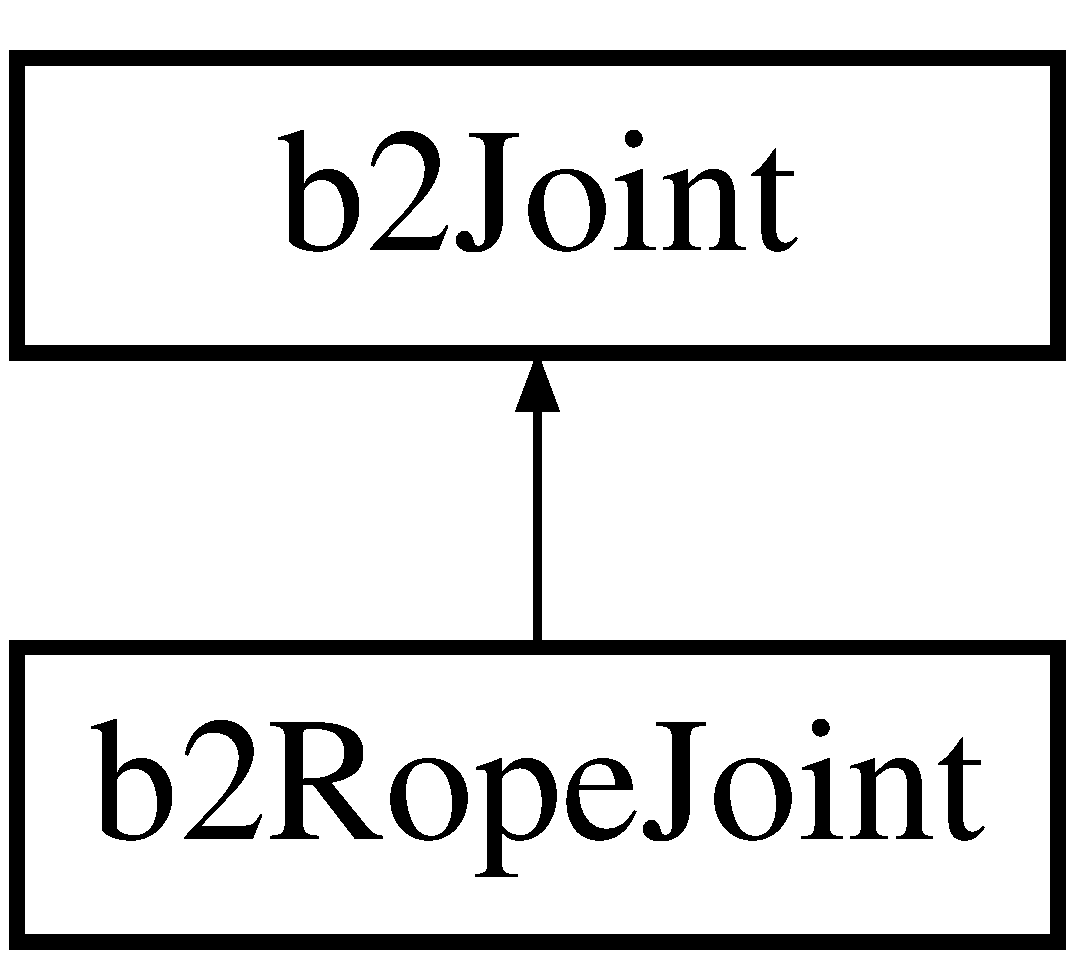
\includegraphics[height=2.000000cm]{classb2RopeJoint}
\end{center}
\end{figure}
\subsection*{Public Member Functions}
\begin{DoxyCompactItemize}
\item 
\mbox{\Hypertarget{classb2RopeJoint_a5757fdeb008bf1bbe15348e80aab9402}\label{classb2RopeJoint_a5757fdeb008bf1bbe15348e80aab9402}} 
\mbox{\hyperlink{structb2Vec2}{b2\+Vec2}} \mbox{\hyperlink{classb2RopeJoint_a5757fdeb008bf1bbe15348e80aab9402}{Get\+AnchorA}} () const override
\begin{DoxyCompactList}\small\item\em Get the anchor point on bodyA in world coordinates. \end{DoxyCompactList}\item 
\mbox{\Hypertarget{classb2RopeJoint_a5e1d615b5cff50b367a74e109184e5d5}\label{classb2RopeJoint_a5e1d615b5cff50b367a74e109184e5d5}} 
\mbox{\hyperlink{structb2Vec2}{b2\+Vec2}} \mbox{\hyperlink{classb2RopeJoint_a5e1d615b5cff50b367a74e109184e5d5}{Get\+AnchorB}} () const override
\begin{DoxyCompactList}\small\item\em Get the anchor point on bodyB in world coordinates. \end{DoxyCompactList}\item 
\mbox{\Hypertarget{classb2RopeJoint_a4637fe7f22383bbc00d23ab4961b1146}\label{classb2RopeJoint_a4637fe7f22383bbc00d23ab4961b1146}} 
\mbox{\hyperlink{structb2Vec2}{b2\+Vec2}} \mbox{\hyperlink{classb2RopeJoint_a4637fe7f22383bbc00d23ab4961b1146}{Get\+Reaction\+Force}} (float32 inv\+\_\+dt) const override
\begin{DoxyCompactList}\small\item\em Get the reaction force on bodyB at the joint anchor in Newtons. \end{DoxyCompactList}\item 
\mbox{\Hypertarget{classb2RopeJoint_ab3d2e29e34ab2fc6a2e23c055d865c18}\label{classb2RopeJoint_ab3d2e29e34ab2fc6a2e23c055d865c18}} 
float32 \mbox{\hyperlink{classb2RopeJoint_ab3d2e29e34ab2fc6a2e23c055d865c18}{Get\+Reaction\+Torque}} (float32 inv\+\_\+dt) const override
\begin{DoxyCompactList}\small\item\em Get the reaction torque on bodyB in N$\ast$m. \end{DoxyCompactList}\item 
\mbox{\Hypertarget{classb2RopeJoint_a5fb600991e676e61e266ecb99448bb86}\label{classb2RopeJoint_a5fb600991e676e61e266ecb99448bb86}} 
const \mbox{\hyperlink{structb2Vec2}{b2\+Vec2}} \& \mbox{\hyperlink{classb2RopeJoint_a5fb600991e676e61e266ecb99448bb86}{Get\+Local\+AnchorA}} () const
\begin{DoxyCompactList}\small\item\em The local anchor point relative to bodyA\textquotesingle{}s origin. \end{DoxyCompactList}\item 
\mbox{\Hypertarget{classb2RopeJoint_a8a9b925c7ffa11d331ba369cc9fe2ac5}\label{classb2RopeJoint_a8a9b925c7ffa11d331ba369cc9fe2ac5}} 
const \mbox{\hyperlink{structb2Vec2}{b2\+Vec2}} \& \mbox{\hyperlink{classb2RopeJoint_a8a9b925c7ffa11d331ba369cc9fe2ac5}{Get\+Local\+AnchorB}} () const
\begin{DoxyCompactList}\small\item\em The local anchor point relative to bodyB\textquotesingle{}s origin. \end{DoxyCompactList}\item 
\mbox{\Hypertarget{classb2RopeJoint_a92cea201d21acd2f2a7cc9b00e165848}\label{classb2RopeJoint_a92cea201d21acd2f2a7cc9b00e165848}} 
void \mbox{\hyperlink{classb2RopeJoint_a92cea201d21acd2f2a7cc9b00e165848}{Set\+Max\+Length}} (float32 length)
\begin{DoxyCompactList}\small\item\em Set/\+Get the maximum length of the rope. \end{DoxyCompactList}\item 
\mbox{\Hypertarget{classb2RopeJoint_abdcc1962f25103a49f6e3f4182559efa}\label{classb2RopeJoint_abdcc1962f25103a49f6e3f4182559efa}} 
float32 {\bfseries Get\+Max\+Length} () const
\item 
\mbox{\Hypertarget{classb2RopeJoint_ab7b606273b65339f0ab502675f32997e}\label{classb2RopeJoint_ab7b606273b65339f0ab502675f32997e}} 
b2\+Limit\+State {\bfseries Get\+Limit\+State} () const
\item 
\mbox{\Hypertarget{classb2RopeJoint_a0028d3d3710bf1a9a905e9b55a4f37c5}\label{classb2RopeJoint_a0028d3d3710bf1a9a905e9b55a4f37c5}} 
void \mbox{\hyperlink{classb2RopeJoint_a0028d3d3710bf1a9a905e9b55a4f37c5}{Dump}} () override
\begin{DoxyCompactList}\small\item\em Dump joint to dm\+Log. \end{DoxyCompactList}\end{DoxyCompactItemize}
\subsection*{Protected Member Functions}
\begin{DoxyCompactItemize}
\item 
\mbox{\Hypertarget{classb2RopeJoint_a3f69f238616d8dc622d9448f81e14e53}\label{classb2RopeJoint_a3f69f238616d8dc622d9448f81e14e53}} 
{\bfseries b2\+Rope\+Joint} (const \mbox{\hyperlink{structb2RopeJointDef}{b2\+Rope\+Joint\+Def}} $\ast$data)
\item 
\mbox{\Hypertarget{classb2RopeJoint_a8a9bd57a12aaf38b529ae626e714e1e8}\label{classb2RopeJoint_a8a9bd57a12aaf38b529ae626e714e1e8}} 
void {\bfseries Init\+Velocity\+Constraints} (const \mbox{\hyperlink{structb2SolverData}{b2\+Solver\+Data}} \&data) override
\item 
\mbox{\Hypertarget{classb2RopeJoint_a08bf8f6cffe281a9f58ee469f99bf5b1}\label{classb2RopeJoint_a08bf8f6cffe281a9f58ee469f99bf5b1}} 
void {\bfseries Solve\+Velocity\+Constraints} (const \mbox{\hyperlink{structb2SolverData}{b2\+Solver\+Data}} \&data) override
\item 
\mbox{\Hypertarget{classb2RopeJoint_a2fcbda6d472c660aa01793c798a8f92e}\label{classb2RopeJoint_a2fcbda6d472c660aa01793c798a8f92e}} 
bool {\bfseries Solve\+Position\+Constraints} (const \mbox{\hyperlink{structb2SolverData}{b2\+Solver\+Data}} \&data) override
\end{DoxyCompactItemize}
\subsection*{Protected Attributes}
\begin{DoxyCompactItemize}
\item 
\mbox{\Hypertarget{classb2RopeJoint_a43640240dc39c912ea1cc6e1ae9fa614}\label{classb2RopeJoint_a43640240dc39c912ea1cc6e1ae9fa614}} 
\mbox{\hyperlink{structb2Vec2}{b2\+Vec2}} {\bfseries m\+\_\+local\+AnchorA}
\item 
\mbox{\Hypertarget{classb2RopeJoint_a57dfab74bae88c2c3284ed640825c959}\label{classb2RopeJoint_a57dfab74bae88c2c3284ed640825c959}} 
\mbox{\hyperlink{structb2Vec2}{b2\+Vec2}} {\bfseries m\+\_\+local\+AnchorB}
\item 
\mbox{\Hypertarget{classb2RopeJoint_ace7528ca1183f34cfc79e47f46b29130}\label{classb2RopeJoint_ace7528ca1183f34cfc79e47f46b29130}} 
float32 {\bfseries m\+\_\+max\+Length}
\item 
\mbox{\Hypertarget{classb2RopeJoint_a2cee8c35d881b0ae66d28d13c6d8d66a}\label{classb2RopeJoint_a2cee8c35d881b0ae66d28d13c6d8d66a}} 
float32 {\bfseries m\+\_\+length}
\item 
\mbox{\Hypertarget{classb2RopeJoint_ac19ae74b5f3c104bc763e99b3986afd6}\label{classb2RopeJoint_ac19ae74b5f3c104bc763e99b3986afd6}} 
float32 {\bfseries m\+\_\+impulse}
\item 
\mbox{\Hypertarget{classb2RopeJoint_a34875f5852d011dab695613a23adca08}\label{classb2RopeJoint_a34875f5852d011dab695613a23adca08}} 
int32 {\bfseries m\+\_\+indexA}
\item 
\mbox{\Hypertarget{classb2RopeJoint_aa67100c069a1a273314dfa55c9063fc7}\label{classb2RopeJoint_aa67100c069a1a273314dfa55c9063fc7}} 
int32 {\bfseries m\+\_\+indexB}
\item 
\mbox{\Hypertarget{classb2RopeJoint_ae95185c5ad4c119a9893294491ba1609}\label{classb2RopeJoint_ae95185c5ad4c119a9893294491ba1609}} 
\mbox{\hyperlink{structb2Vec2}{b2\+Vec2}} {\bfseries m\+\_\+u}
\item 
\mbox{\Hypertarget{classb2RopeJoint_af8ae48af2656b1e605a099b8f4aa82b0}\label{classb2RopeJoint_af8ae48af2656b1e605a099b8f4aa82b0}} 
\mbox{\hyperlink{structb2Vec2}{b2\+Vec2}} {\bfseries m\+\_\+rA}
\item 
\mbox{\Hypertarget{classb2RopeJoint_ae577e49beef03d266ff4c54e852b4f41}\label{classb2RopeJoint_ae577e49beef03d266ff4c54e852b4f41}} 
\mbox{\hyperlink{structb2Vec2}{b2\+Vec2}} {\bfseries m\+\_\+rB}
\item 
\mbox{\Hypertarget{classb2RopeJoint_a15ff1472deb6405c9886a40ee99efcef}\label{classb2RopeJoint_a15ff1472deb6405c9886a40ee99efcef}} 
\mbox{\hyperlink{structb2Vec2}{b2\+Vec2}} {\bfseries m\+\_\+local\+CenterA}
\item 
\mbox{\Hypertarget{classb2RopeJoint_a2b3b1ac9ae9e3e68b2550809ec178877}\label{classb2RopeJoint_a2b3b1ac9ae9e3e68b2550809ec178877}} 
\mbox{\hyperlink{structb2Vec2}{b2\+Vec2}} {\bfseries m\+\_\+local\+CenterB}
\item 
\mbox{\Hypertarget{classb2RopeJoint_a690e4fe5ab7a279accac3b137d5f5c76}\label{classb2RopeJoint_a690e4fe5ab7a279accac3b137d5f5c76}} 
float32 {\bfseries m\+\_\+inv\+MassA}
\item 
\mbox{\Hypertarget{classb2RopeJoint_a9709179725abed80d4957df82bc24512}\label{classb2RopeJoint_a9709179725abed80d4957df82bc24512}} 
float32 {\bfseries m\+\_\+inv\+MassB}
\item 
\mbox{\Hypertarget{classb2RopeJoint_a1917a65b89668c433d06071970a6875a}\label{classb2RopeJoint_a1917a65b89668c433d06071970a6875a}} 
float32 {\bfseries m\+\_\+inv\+IA}
\item 
\mbox{\Hypertarget{classb2RopeJoint_a1ce440194cec6e275193d7224ce1e448}\label{classb2RopeJoint_a1ce440194cec6e275193d7224ce1e448}} 
float32 {\bfseries m\+\_\+inv\+IB}
\item 
\mbox{\Hypertarget{classb2RopeJoint_a1f355a976b177b75a8fd47190194d5c1}\label{classb2RopeJoint_a1f355a976b177b75a8fd47190194d5c1}} 
float32 {\bfseries m\+\_\+mass}
\item 
\mbox{\Hypertarget{classb2RopeJoint_ac73c9451360c80c8a98376b922f4bed4}\label{classb2RopeJoint_ac73c9451360c80c8a98376b922f4bed4}} 
b2\+Limit\+State {\bfseries m\+\_\+state}
\end{DoxyCompactItemize}
\subsection*{Friends}
\begin{DoxyCompactItemize}
\item 
\mbox{\Hypertarget{classb2RopeJoint_a54ade8ed3d794298108d7f4c4e4793fa}\label{classb2RopeJoint_a54ade8ed3d794298108d7f4c4e4793fa}} 
class {\bfseries b2\+Joint}
\end{DoxyCompactItemize}
\subsection*{Additional Inherited Members}


\subsection{Detailed Description}
A rope joint enforces a maximum distance between two points on two bodies. It has no other effect. Warning\+: if you attempt to change the maximum length during the simulation you will get some non-\/physical behavior. A model that would allow you to dynamically modify the length would have some sponginess, so I chose not to implement it that way. See \mbox{\hyperlink{classb2DistanceJoint}{b2\+Distance\+Joint}} if you want to dynamically control length. 

The documentation for this class was generated from the following files\+:\begin{DoxyCompactItemize}
\item 
Dynamics/\+Joints/b2\+Rope\+Joint.\+h\item 
Dynamics/\+Joints/b2\+Rope\+Joint.\+cpp\end{DoxyCompactItemize}

\hypertarget{structb2RopeJointDef}{}\section{b2\+Rope\+Joint\+Def Struct Reference}
\label{structb2RopeJointDef}\index{b2\+Rope\+Joint\+Def@{b2\+Rope\+Joint\+Def}}


{\ttfamily \#include $<$b2\+Rope\+Joint.\+h$>$}

Inheritance diagram for b2\+Rope\+Joint\+Def\+:\begin{figure}[H]
\begin{center}
\leavevmode
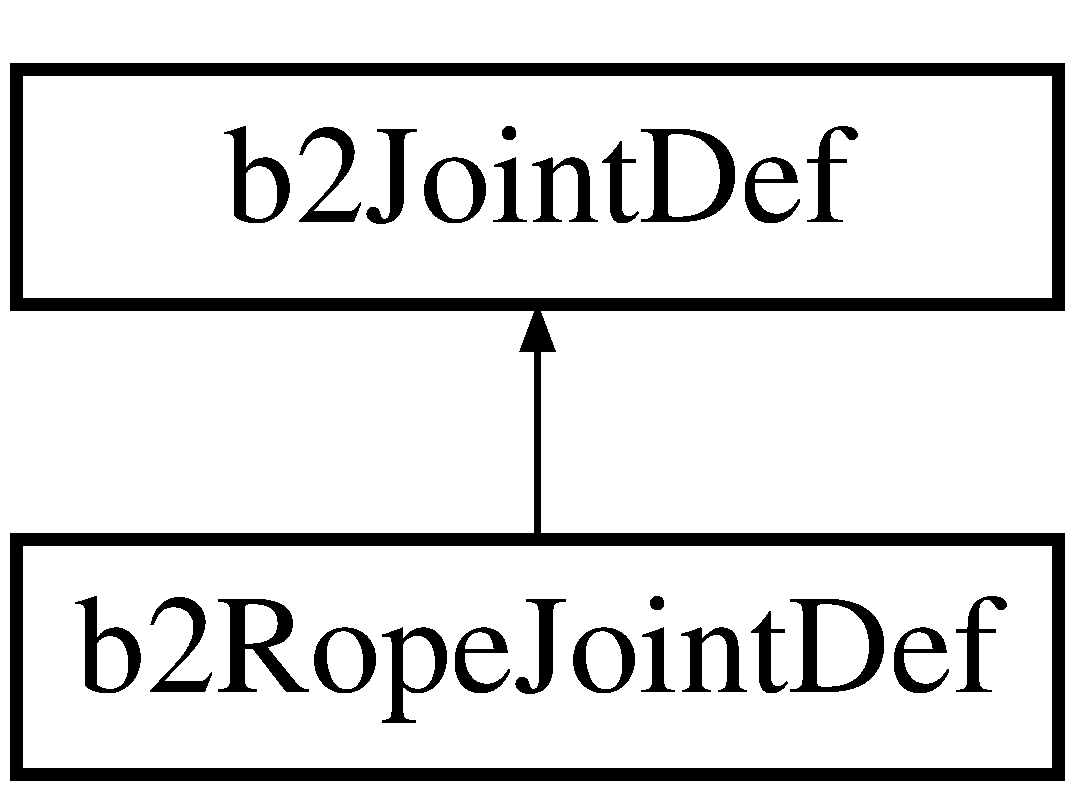
\includegraphics[height=2.000000cm]{structb2RopeJointDef}
\end{center}
\end{figure}
\subsection*{Public Attributes}
\begin{DoxyCompactItemize}
\item 
\mbox{\Hypertarget{structb2RopeJointDef_ab680fcc3cd44741a7a824ddff86ff01e}\label{structb2RopeJointDef_ab680fcc3cd44741a7a824ddff86ff01e}} 
\mbox{\hyperlink{structb2Vec2}{b2\+Vec2}} \mbox{\hyperlink{structb2RopeJointDef_ab680fcc3cd44741a7a824ddff86ff01e}{local\+AnchorA}}
\begin{DoxyCompactList}\small\item\em The local anchor point relative to bodyA\textquotesingle{}s origin. \end{DoxyCompactList}\item 
\mbox{\Hypertarget{structb2RopeJointDef_a3271da0e4027e25546aa6a81e8fbe4e2}\label{structb2RopeJointDef_a3271da0e4027e25546aa6a81e8fbe4e2}} 
\mbox{\hyperlink{structb2Vec2}{b2\+Vec2}} \mbox{\hyperlink{structb2RopeJointDef_a3271da0e4027e25546aa6a81e8fbe4e2}{local\+AnchorB}}
\begin{DoxyCompactList}\small\item\em The local anchor point relative to bodyB\textquotesingle{}s origin. \end{DoxyCompactList}\item 
float32 \mbox{\hyperlink{structb2RopeJointDef_a6efdcae22e2bdcfc3aae62da1a5f0d69}{max\+Length}}
\end{DoxyCompactItemize}


\subsection{Detailed Description}
Rope joint definition. This requires two body anchor points and a maximum lengths. Note\+: by default the connected objects will not collide. see collide\+Connected in \mbox{\hyperlink{structb2JointDef}{b2\+Joint\+Def}}. 

\subsection{Member Data Documentation}
\mbox{\Hypertarget{structb2RopeJointDef_a6efdcae22e2bdcfc3aae62da1a5f0d69}\label{structb2RopeJointDef_a6efdcae22e2bdcfc3aae62da1a5f0d69}} 
\index{b2\+Rope\+Joint\+Def@{b2\+Rope\+Joint\+Def}!max\+Length@{max\+Length}}
\index{max\+Length@{max\+Length}!b2\+Rope\+Joint\+Def@{b2\+Rope\+Joint\+Def}}
\subsubsection{\texorpdfstring{max\+Length}{maxLength}}
{\footnotesize\ttfamily float32 b2\+Rope\+Joint\+Def\+::max\+Length}

The maximum length of the rope. Warning\+: this must be larger than b2\+\_\+linear\+Slop or the joint will have no effect. 

The documentation for this struct was generated from the following file\+:\begin{DoxyCompactItemize}
\item 
Dynamics/\+Joints/b2\+Rope\+Joint.\+h\end{DoxyCompactItemize}

\hypertarget{structb2Rot}{}\section{b2\+Rot Struct Reference}
\label{structb2Rot}\index{b2\+Rot@{b2\+Rot}}


Rotation.  




{\ttfamily \#include $<$b2\+Math.\+h$>$}

\subsection*{Public Member Functions}
\begin{DoxyCompactItemize}
\item 
\mbox{\hyperlink{structb2Rot_aa40dda6d390a2f54c793c63027a9b46e}{b2\+Rot}} (float32 angle)
\begin{DoxyCompactList}\small\item\em Initialize from an angle in radians. \end{DoxyCompactList}\item 
void \mbox{\hyperlink{structb2Rot_acde9186de0a4a7397bf8ef714408ad60}{Set}} (float32 angle)
\begin{DoxyCompactList}\small\item\em Set using an angle in radians. \end{DoxyCompactList}\item 
\mbox{\Hypertarget{structb2Rot_a7f534cb7ece8d325662d7d0e27d4f617}\label{structb2Rot_a7f534cb7ece8d325662d7d0e27d4f617}} 
void \mbox{\hyperlink{structb2Rot_a7f534cb7ece8d325662d7d0e27d4f617}{Set\+Identity}} ()
\begin{DoxyCompactList}\small\item\em Set to the identity rotation. \end{DoxyCompactList}\item 
\mbox{\Hypertarget{structb2Rot_a45031fccfa11d3b3a09154008ce28b39}\label{structb2Rot_a45031fccfa11d3b3a09154008ce28b39}} 
float32 \mbox{\hyperlink{structb2Rot_a45031fccfa11d3b3a09154008ce28b39}{Get\+Angle}} () const
\begin{DoxyCompactList}\small\item\em Get the angle in radians. \end{DoxyCompactList}\item 
\mbox{\Hypertarget{structb2Rot_a952a5555c1f68ce3e39ac992fcf4eba9}\label{structb2Rot_a952a5555c1f68ce3e39ac992fcf4eba9}} 
\mbox{\hyperlink{structb2Vec2}{b2\+Vec2}} \mbox{\hyperlink{structb2Rot_a952a5555c1f68ce3e39ac992fcf4eba9}{Get\+X\+Axis}} () const
\begin{DoxyCompactList}\small\item\em Get the x-\/axis. \end{DoxyCompactList}\item 
\mbox{\Hypertarget{structb2Rot_ab057c4e9dc821099949391a6ded36dd6}\label{structb2Rot_ab057c4e9dc821099949391a6ded36dd6}} 
\mbox{\hyperlink{structb2Vec2}{b2\+Vec2}} \mbox{\hyperlink{structb2Rot_ab057c4e9dc821099949391a6ded36dd6}{Get\+Y\+Axis}} () const
\begin{DoxyCompactList}\small\item\em Get the u-\/axis. \end{DoxyCompactList}\end{DoxyCompactItemize}
\subsection*{Public Attributes}
\begin{DoxyCompactItemize}
\item 
\mbox{\Hypertarget{structb2Rot_a15725ce0a89cc735ad90687b4c0f4dce}\label{structb2Rot_a15725ce0a89cc735ad90687b4c0f4dce}} 
float32 \mbox{\hyperlink{structb2Rot_a15725ce0a89cc735ad90687b4c0f4dce}{s}}
\begin{DoxyCompactList}\small\item\em Sine and cosine. \end{DoxyCompactList}\item 
\mbox{\Hypertarget{structb2Rot_af23e5d31889dcb806ce46ce55aa81261}\label{structb2Rot_af23e5d31889dcb806ce46ce55aa81261}} 
float32 {\bfseries c}
\end{DoxyCompactItemize}


\subsection{Detailed Description}
Rotation. 

\subsection{Constructor \& Destructor Documentation}
\mbox{\Hypertarget{structb2Rot_aa40dda6d390a2f54c793c63027a9b46e}\label{structb2Rot_aa40dda6d390a2f54c793c63027a9b46e}} 
\index{b2\+Rot@{b2\+Rot}!b2\+Rot@{b2\+Rot}}
\index{b2\+Rot@{b2\+Rot}!b2\+Rot@{b2\+Rot}}
\subsubsection{\texorpdfstring{b2\+Rot()}{b2Rot()}}
{\footnotesize\ttfamily b2\+Rot\+::b2\+Rot (\begin{DoxyParamCaption}\item[{float32}]{angle }\end{DoxyParamCaption})\hspace{0.3cm}{\ttfamily [inline]}, {\ttfamily [explicit]}}



Initialize from an angle in radians. 

T\+O\+D\+O\+\_\+\+E\+R\+IN optimize 

\subsection{Member Function Documentation}
\mbox{\Hypertarget{structb2Rot_acde9186de0a4a7397bf8ef714408ad60}\label{structb2Rot_acde9186de0a4a7397bf8ef714408ad60}} 
\index{b2\+Rot@{b2\+Rot}!Set@{Set}}
\index{Set@{Set}!b2\+Rot@{b2\+Rot}}
\subsubsection{\texorpdfstring{Set()}{Set()}}
{\footnotesize\ttfamily void b2\+Rot\+::\+Set (\begin{DoxyParamCaption}\item[{float32}]{angle }\end{DoxyParamCaption})\hspace{0.3cm}{\ttfamily [inline]}}



Set using an angle in radians. 

T\+O\+D\+O\+\_\+\+E\+R\+IN optimize 

The documentation for this struct was generated from the following file\+:\begin{DoxyCompactItemize}
\item 
Common/b2\+Math.\+h\end{DoxyCompactItemize}

\hypertarget{structb2SeparationFunction}{}\section{b2\+Separation\+Function Struct Reference}
\label{structb2SeparationFunction}\index{b2\+Separation\+Function@{b2\+Separation\+Function}}
\subsection*{Public Types}
\begin{DoxyCompactItemize}
\item 
\mbox{\Hypertarget{structb2SeparationFunction_a8c1446894223e9b6c80dc4d7230141a4}\label{structb2SeparationFunction_a8c1446894223e9b6c80dc4d7230141a4}} 
enum {\bfseries Type} \{ {\bfseries e\+\_\+points}, 
{\bfseries e\+\_\+faceA}, 
{\bfseries e\+\_\+faceB}
 \}
\end{DoxyCompactItemize}
\subsection*{Public Member Functions}
\begin{DoxyCompactItemize}
\item 
\mbox{\Hypertarget{structb2SeparationFunction_acfe0bb0d85a5001f1e957eea2137e039}\label{structb2SeparationFunction_acfe0bb0d85a5001f1e957eea2137e039}} 
float32 {\bfseries Initialize} (const \mbox{\hyperlink{structb2SimplexCache}{b2\+Simplex\+Cache}} $\ast$cache, const \mbox{\hyperlink{structb2DistanceProxy}{b2\+Distance\+Proxy}} $\ast$proxyA, const \mbox{\hyperlink{structb2Sweep}{b2\+Sweep}} \&sweepA, const \mbox{\hyperlink{structb2DistanceProxy}{b2\+Distance\+Proxy}} $\ast$proxyB, const \mbox{\hyperlink{structb2Sweep}{b2\+Sweep}} \&sweepB, float32 t1)
\item 
\mbox{\Hypertarget{structb2SeparationFunction_ac0a603a96343be37d0a0bdf852be1e77}\label{structb2SeparationFunction_ac0a603a96343be37d0a0bdf852be1e77}} 
float32 {\bfseries Find\+Min\+Separation} (int32 $\ast$indexA, int32 $\ast$indexB, float32 t) const
\item 
\mbox{\Hypertarget{structb2SeparationFunction_a68224ac8a89b10a9d1b39789ccc78d4c}\label{structb2SeparationFunction_a68224ac8a89b10a9d1b39789ccc78d4c}} 
float32 {\bfseries Evaluate} (int32 indexA, int32 indexB, float32 t) const
\end{DoxyCompactItemize}
\subsection*{Public Attributes}
\begin{DoxyCompactItemize}
\item 
\mbox{\Hypertarget{structb2SeparationFunction_a5c03d798e97cd653aa7db390275bf9a7}\label{structb2SeparationFunction_a5c03d798e97cd653aa7db390275bf9a7}} 
const \mbox{\hyperlink{structb2DistanceProxy}{b2\+Distance\+Proxy}} $\ast$ {\bfseries m\+\_\+proxyA}
\item 
\mbox{\Hypertarget{structb2SeparationFunction_a25fc938e03bf77ac276b17b24e52958f}\label{structb2SeparationFunction_a25fc938e03bf77ac276b17b24e52958f}} 
const \mbox{\hyperlink{structb2DistanceProxy}{b2\+Distance\+Proxy}} $\ast$ {\bfseries m\+\_\+proxyB}
\item 
\mbox{\Hypertarget{structb2SeparationFunction_a46b838a661baa40cde771b779c2ff341}\label{structb2SeparationFunction_a46b838a661baa40cde771b779c2ff341}} 
\mbox{\hyperlink{structb2Sweep}{b2\+Sweep}} {\bfseries m\+\_\+sweepA}
\item 
\mbox{\Hypertarget{structb2SeparationFunction_a11ba433f6e524fb92390bd8b4dd376b6}\label{structb2SeparationFunction_a11ba433f6e524fb92390bd8b4dd376b6}} 
\mbox{\hyperlink{structb2Sweep}{b2\+Sweep}} {\bfseries m\+\_\+sweepB}
\item 
\mbox{\Hypertarget{structb2SeparationFunction_a51075eff2de404a1d82eee831fdfd4af}\label{structb2SeparationFunction_a51075eff2de404a1d82eee831fdfd4af}} 
Type {\bfseries m\+\_\+type}
\item 
\mbox{\Hypertarget{structb2SeparationFunction_ab77a17de0f5c708212090f599ec1795e}\label{structb2SeparationFunction_ab77a17de0f5c708212090f599ec1795e}} 
\mbox{\hyperlink{structb2Vec2}{b2\+Vec2}} {\bfseries m\+\_\+local\+Point}
\item 
\mbox{\Hypertarget{structb2SeparationFunction_a767b8fc4174d200ae8fb1d2bfba3407b}\label{structb2SeparationFunction_a767b8fc4174d200ae8fb1d2bfba3407b}} 
\mbox{\hyperlink{structb2Vec2}{b2\+Vec2}} {\bfseries m\+\_\+axis}
\end{DoxyCompactItemize}


The documentation for this struct was generated from the following file\+:\begin{DoxyCompactItemize}
\item 
Collision/b2\+Time\+Of\+Impact.\+cpp\end{DoxyCompactItemize}

\hypertarget{classb2Shape}{}\section{b2\+Shape Class Reference}
\label{classb2Shape}\index{b2\+Shape@{b2\+Shape}}


{\ttfamily \#include $<$b2\+Shape.\+h$>$}

Inheritance diagram for b2\+Shape\+:\begin{figure}[H]
\begin{center}
\leavevmode
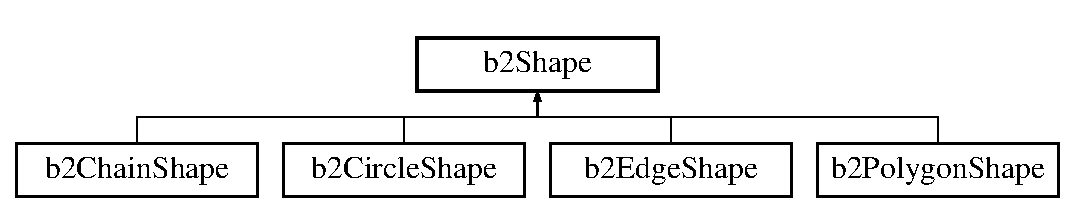
\includegraphics[height=2.000000cm]{classb2Shape}
\end{center}
\end{figure}
\subsection*{Public Types}
\begin{DoxyCompactItemize}
\item 
\mbox{\Hypertarget{classb2Shape_a4c1f3a9ad6b3150bb90ad9018ca4b1e0}\label{classb2Shape_a4c1f3a9ad6b3150bb90ad9018ca4b1e0}} 
enum {\bfseries Type} \{ \newline
{\bfseries e\+\_\+circle} = 0, 
{\bfseries e\+\_\+edge} = 1, 
{\bfseries e\+\_\+polygon} = 2, 
{\bfseries e\+\_\+chain} = 3, 
\newline
{\bfseries e\+\_\+type\+Count} = 4
 \}
\end{DoxyCompactItemize}
\subsection*{Public Member Functions}
\begin{DoxyCompactItemize}
\item 
\mbox{\Hypertarget{classb2Shape_a4716243454bb9cf7c7ee1d9cb23ae634}\label{classb2Shape_a4716243454bb9cf7c7ee1d9cb23ae634}} 
virtual \mbox{\hyperlink{classb2Shape}{b2\+Shape}} $\ast$ \mbox{\hyperlink{classb2Shape_a4716243454bb9cf7c7ee1d9cb23ae634}{Clone}} (\mbox{\hyperlink{classb2BlockAllocator}{b2\+Block\+Allocator}} $\ast$allocator) const =0
\begin{DoxyCompactList}\small\item\em Clone the concrete shape using the provided allocator. \end{DoxyCompactList}\item 
Type \mbox{\hyperlink{classb2Shape_a600cceee6186d81bb1b8ab142324bba6}{Get\+Type}} () const
\item 
\mbox{\Hypertarget{classb2Shape_a05a3c445017d96df9238ceefe6ce37ab}\label{classb2Shape_a05a3c445017d96df9238ceefe6ce37ab}} 
virtual int32 \mbox{\hyperlink{classb2Shape_a05a3c445017d96df9238ceefe6ce37ab}{Get\+Child\+Count}} () const =0
\begin{DoxyCompactList}\small\item\em Get the number of child primitives. \end{DoxyCompactList}\item 
virtual bool \mbox{\hyperlink{classb2Shape_a6ac968e403e2d93e8ae46d728a2e50fa}{Test\+Point}} (const \mbox{\hyperlink{structb2Transform}{b2\+Transform}} \&xf, const \mbox{\hyperlink{structb2Vec2}{b2\+Vec2}} \&p) const =0
\item 
virtual bool \mbox{\hyperlink{classb2Shape_aee53a926f4fe64cd03693f6211ef6335}{Ray\+Cast}} (\mbox{\hyperlink{structb2RayCastOutput}{b2\+Ray\+Cast\+Output}} $\ast$output, const \mbox{\hyperlink{structb2RayCastInput}{b2\+Ray\+Cast\+Input}} \&input, const \mbox{\hyperlink{structb2Transform}{b2\+Transform}} \&transform, int32 child\+Index) const =0
\item 
virtual void \mbox{\hyperlink{classb2Shape_a88e9807fab0c8ca9a98d8926e50a1411}{Compute\+A\+A\+BB}} (\mbox{\hyperlink{structb2AABB}{b2\+A\+A\+BB}} $\ast$aabb, const \mbox{\hyperlink{structb2Transform}{b2\+Transform}} \&xf, int32 child\+Index) const =0
\item 
virtual void \mbox{\hyperlink{classb2Shape_a61b365526241b47f124789b0309cac69}{Compute\+Mass}} (\mbox{\hyperlink{structb2MassData}{b2\+Mass\+Data}} $\ast$mass\+Data, float32 density) const =0
\end{DoxyCompactItemize}
\subsection*{Public Attributes}
\begin{DoxyCompactItemize}
\item 
\mbox{\Hypertarget{classb2Shape_adb051791133b24f53c6e9a565a7b7bbb}\label{classb2Shape_adb051791133b24f53c6e9a565a7b7bbb}} 
Type {\bfseries m\+\_\+type}
\item 
float32 \mbox{\hyperlink{classb2Shape_a5de7a9bd3f9e72ef7025a65c304aaf1a}{m\+\_\+radius}}
\end{DoxyCompactItemize}


\subsection{Detailed Description}
A shape is used for collision detection. You can create a shape however you like. Shapes used for simulation in \mbox{\hyperlink{classb2World}{b2\+World}} are created automatically when a \mbox{\hyperlink{classb2Fixture}{b2\+Fixture}} is created. Shapes may encapsulate a one or more child shapes. 

\subsection{Member Function Documentation}
\mbox{\Hypertarget{classb2Shape_a88e9807fab0c8ca9a98d8926e50a1411}\label{classb2Shape_a88e9807fab0c8ca9a98d8926e50a1411}} 
\index{b2\+Shape@{b2\+Shape}!Compute\+A\+A\+BB@{Compute\+A\+A\+BB}}
\index{Compute\+A\+A\+BB@{Compute\+A\+A\+BB}!b2\+Shape@{b2\+Shape}}
\subsubsection{\texorpdfstring{Compute\+A\+A\+B\+B()}{ComputeAABB()}}
{\footnotesize\ttfamily virtual void b2\+Shape\+::\+Compute\+A\+A\+BB (\begin{DoxyParamCaption}\item[{\mbox{\hyperlink{structb2AABB}{b2\+A\+A\+BB}} $\ast$}]{aabb,  }\item[{const \mbox{\hyperlink{structb2Transform}{b2\+Transform}} \&}]{xf,  }\item[{int32}]{child\+Index }\end{DoxyParamCaption}) const\hspace{0.3cm}{\ttfamily [pure virtual]}}

Given a transform, compute the associated axis aligned bounding box for a child shape. 
\begin{DoxyParams}{Parameters}
{\em aabb} & returns the axis aligned box. \\
\hline
{\em xf} & the world transform of the shape. \\
\hline
{\em child\+Index} & the child shape \\
\hline
\end{DoxyParams}


Implemented in \mbox{\hyperlink{classb2ChainShape_ae1d7470ce8d32e92d27c149ab45f5468}{b2\+Chain\+Shape}}, \mbox{\hyperlink{classb2PolygonShape_ae9bcc185caf4a030003cefc4576e4717}{b2\+Polygon\+Shape}}, \mbox{\hyperlink{classb2EdgeShape_a238139ae1736b457d77443133ff16854}{b2\+Edge\+Shape}}, and \mbox{\hyperlink{classb2CircleShape_af4a4ea78780af7a7ce40bf5d54affe83}{b2\+Circle\+Shape}}.

\mbox{\Hypertarget{classb2Shape_a61b365526241b47f124789b0309cac69}\label{classb2Shape_a61b365526241b47f124789b0309cac69}} 
\index{b2\+Shape@{b2\+Shape}!Compute\+Mass@{Compute\+Mass}}
\index{Compute\+Mass@{Compute\+Mass}!b2\+Shape@{b2\+Shape}}
\subsubsection{\texorpdfstring{Compute\+Mass()}{ComputeMass()}}
{\footnotesize\ttfamily virtual void b2\+Shape\+::\+Compute\+Mass (\begin{DoxyParamCaption}\item[{\mbox{\hyperlink{structb2MassData}{b2\+Mass\+Data}} $\ast$}]{mass\+Data,  }\item[{float32}]{density }\end{DoxyParamCaption}) const\hspace{0.3cm}{\ttfamily [pure virtual]}}

Compute the mass properties of this shape using its dimensions and density. The inertia tensor is computed about the local origin. 
\begin{DoxyParams}{Parameters}
{\em mass\+Data} & returns the mass data for this shape. \\
\hline
{\em density} & the density in kilograms per meter squared. \\
\hline
\end{DoxyParams}


Implemented in \mbox{\hyperlink{classb2ChainShape_aad3671d6eab61f6b26e2f1b6ac50bb98}{b2\+Chain\+Shape}}, \mbox{\hyperlink{classb2PolygonShape_a908db2a51fc79fd49d6fe06be2cd8474}{b2\+Polygon\+Shape}}, \mbox{\hyperlink{classb2EdgeShape_ac738c1e0ab2f4dfbab26e3942efa60af}{b2\+Edge\+Shape}}, and \mbox{\hyperlink{classb2CircleShape_a7dc07891abd015863fbf03076e47eec5}{b2\+Circle\+Shape}}.

\mbox{\Hypertarget{classb2Shape_a600cceee6186d81bb1b8ab142324bba6}\label{classb2Shape_a600cceee6186d81bb1b8ab142324bba6}} 
\index{b2\+Shape@{b2\+Shape}!Get\+Type@{Get\+Type}}
\index{Get\+Type@{Get\+Type}!b2\+Shape@{b2\+Shape}}
\subsubsection{\texorpdfstring{Get\+Type()}{GetType()}}
{\footnotesize\ttfamily b2\+Shape\+::\+Type b2\+Shape\+::\+Get\+Type (\begin{DoxyParamCaption}{ }\end{DoxyParamCaption}) const\hspace{0.3cm}{\ttfamily [inline]}}

Get the type of this shape. You can use this to down cast to the concrete shape. \begin{DoxyReturn}{Returns}
the shape type. 
\end{DoxyReturn}
\mbox{\Hypertarget{classb2Shape_aee53a926f4fe64cd03693f6211ef6335}\label{classb2Shape_aee53a926f4fe64cd03693f6211ef6335}} 
\index{b2\+Shape@{b2\+Shape}!Ray\+Cast@{Ray\+Cast}}
\index{Ray\+Cast@{Ray\+Cast}!b2\+Shape@{b2\+Shape}}
\subsubsection{\texorpdfstring{Ray\+Cast()}{RayCast()}}
{\footnotesize\ttfamily virtual bool b2\+Shape\+::\+Ray\+Cast (\begin{DoxyParamCaption}\item[{\mbox{\hyperlink{structb2RayCastOutput}{b2\+Ray\+Cast\+Output}} $\ast$}]{output,  }\item[{const \mbox{\hyperlink{structb2RayCastInput}{b2\+Ray\+Cast\+Input}} \&}]{input,  }\item[{const \mbox{\hyperlink{structb2Transform}{b2\+Transform}} \&}]{transform,  }\item[{int32}]{child\+Index }\end{DoxyParamCaption}) const\hspace{0.3cm}{\ttfamily [pure virtual]}}

Cast a ray against a child shape. 
\begin{DoxyParams}{Parameters}
{\em output} & the ray-\/cast results. \\
\hline
{\em input} & the ray-\/cast input parameters. \\
\hline
{\em transform} & the transform to be applied to the shape. \\
\hline
{\em child\+Index} & the child shape index \\
\hline
\end{DoxyParams}


Implemented in \mbox{\hyperlink{classb2ChainShape_add9e88f7f90b32ae75738cfb042ef532}{b2\+Chain\+Shape}}, \mbox{\hyperlink{classb2PolygonShape_a41f20072763688f1745f12f67f40e904}{b2\+Polygon\+Shape}}, \mbox{\hyperlink{classb2EdgeShape_a192cf10bd556a5a90b29a2bcee2ddd75}{b2\+Edge\+Shape}}, and \mbox{\hyperlink{classb2CircleShape_a442e847b9fc3d1344b02b48d490eb0c6}{b2\+Circle\+Shape}}.

\mbox{\Hypertarget{classb2Shape_a6ac968e403e2d93e8ae46d728a2e50fa}\label{classb2Shape_a6ac968e403e2d93e8ae46d728a2e50fa}} 
\index{b2\+Shape@{b2\+Shape}!Test\+Point@{Test\+Point}}
\index{Test\+Point@{Test\+Point}!b2\+Shape@{b2\+Shape}}
\subsubsection{\texorpdfstring{Test\+Point()}{TestPoint()}}
{\footnotesize\ttfamily virtual bool b2\+Shape\+::\+Test\+Point (\begin{DoxyParamCaption}\item[{const \mbox{\hyperlink{structb2Transform}{b2\+Transform}} \&}]{xf,  }\item[{const \mbox{\hyperlink{structb2Vec2}{b2\+Vec2}} \&}]{p }\end{DoxyParamCaption}) const\hspace{0.3cm}{\ttfamily [pure virtual]}}

Test a point for containment in this shape. This only works for convex shapes. 
\begin{DoxyParams}{Parameters}
{\em xf} & the shape world transform. \\
\hline
{\em p} & a point in world coordinates. \\
\hline
\end{DoxyParams}


Implemented in \mbox{\hyperlink{classb2ChainShape_afd03c8679f18f9962a6c76bde629c62a}{b2\+Chain\+Shape}}, \mbox{\hyperlink{classb2PolygonShape_a129c4ac76727fe02724f675e3fef7fe5}{b2\+Polygon\+Shape}}, \mbox{\hyperlink{classb2EdgeShape_a15151673cf9ad585779c70363425f470}{b2\+Edge\+Shape}}, and \mbox{\hyperlink{classb2CircleShape_a84e22b3807e84b72f2981010fc197099}{b2\+Circle\+Shape}}.



\subsection{Member Data Documentation}
\mbox{\Hypertarget{classb2Shape_a5de7a9bd3f9e72ef7025a65c304aaf1a}\label{classb2Shape_a5de7a9bd3f9e72ef7025a65c304aaf1a}} 
\index{b2\+Shape@{b2\+Shape}!m\+\_\+radius@{m\+\_\+radius}}
\index{m\+\_\+radius@{m\+\_\+radius}!b2\+Shape@{b2\+Shape}}
\subsubsection{\texorpdfstring{m\+\_\+radius}{m\_radius}}
{\footnotesize\ttfamily float32 b2\+Shape\+::m\+\_\+radius}

Radius of a shape. For polygonal shapes this must be b2\+\_\+polygon\+Radius. There is no support for making rounded polygons. 

The documentation for this class was generated from the following file\+:\begin{DoxyCompactItemize}
\item 
Collision/\+Shapes/b2\+Shape.\+h\end{DoxyCompactItemize}

\hypertarget{structb2Simplex}{}\section{b2\+Simplex Struct Reference}
\label{structb2Simplex}\index{b2\+Simplex@{b2\+Simplex}}
\subsection*{Public Member Functions}
\begin{DoxyCompactItemize}
\item 
\mbox{\Hypertarget{structb2Simplex_ada29ffb34774589d2e4686316104ddbc}\label{structb2Simplex_ada29ffb34774589d2e4686316104ddbc}} 
void {\bfseries Read\+Cache} (const \mbox{\hyperlink{structb2SimplexCache}{b2\+Simplex\+Cache}} $\ast$cache, const \mbox{\hyperlink{structb2DistanceProxy}{b2\+Distance\+Proxy}} $\ast$proxyA, const \mbox{\hyperlink{structb2Transform}{b2\+Transform}} \&transformA, const \mbox{\hyperlink{structb2DistanceProxy}{b2\+Distance\+Proxy}} $\ast$proxyB, const \mbox{\hyperlink{structb2Transform}{b2\+Transform}} \&transformB)
\item 
\mbox{\Hypertarget{structb2Simplex_a8161f17ee71e0620b63842a05776dd4b}\label{structb2Simplex_a8161f17ee71e0620b63842a05776dd4b}} 
void {\bfseries Write\+Cache} (\mbox{\hyperlink{structb2SimplexCache}{b2\+Simplex\+Cache}} $\ast$cache) const
\item 
\mbox{\Hypertarget{structb2Simplex_af29facd0f4138b32929b575e74ecabd9}\label{structb2Simplex_af29facd0f4138b32929b575e74ecabd9}} 
\mbox{\hyperlink{structb2Vec2}{b2\+Vec2}} {\bfseries Get\+Search\+Direction} () const
\item 
\mbox{\Hypertarget{structb2Simplex_a2044bf067dd5f65d63f96ca6e1dded45}\label{structb2Simplex_a2044bf067dd5f65d63f96ca6e1dded45}} 
\mbox{\hyperlink{structb2Vec2}{b2\+Vec2}} {\bfseries Get\+Closest\+Point} () const
\item 
\mbox{\Hypertarget{structb2Simplex_ac0ce6596bc03509851efb79e8824c1cd}\label{structb2Simplex_ac0ce6596bc03509851efb79e8824c1cd}} 
void {\bfseries Get\+Witness\+Points} (\mbox{\hyperlink{structb2Vec2}{b2\+Vec2}} $\ast$pA, \mbox{\hyperlink{structb2Vec2}{b2\+Vec2}} $\ast$pB) const
\item 
\mbox{\Hypertarget{structb2Simplex_a9ca3fb6a480b36f80c3eadfb2b387d02}\label{structb2Simplex_a9ca3fb6a480b36f80c3eadfb2b387d02}} 
float32 {\bfseries Get\+Metric} () const
\item 
\mbox{\Hypertarget{structb2Simplex_a449fa9b3f63d7f49535dfe9767f1b9bd}\label{structb2Simplex_a449fa9b3f63d7f49535dfe9767f1b9bd}} 
void {\bfseries Solve2} ()
\item 
\mbox{\Hypertarget{structb2Simplex_a7835361343a7388b8f15c94c8deb48c6}\label{structb2Simplex_a7835361343a7388b8f15c94c8deb48c6}} 
void {\bfseries Solve3} ()
\end{DoxyCompactItemize}
\subsection*{Public Attributes}
\begin{DoxyCompactItemize}
\item 
\mbox{\Hypertarget{structb2Simplex_a974d030fe572112e6d5212520586eb13}\label{structb2Simplex_a974d030fe572112e6d5212520586eb13}} 
\mbox{\hyperlink{structb2SimplexVertex}{b2\+Simplex\+Vertex}} {\bfseries m\+\_\+v1}
\item 
\mbox{\Hypertarget{structb2Simplex_a1732c0f9d63e7cdbd405e7a7b2c7b7cb}\label{structb2Simplex_a1732c0f9d63e7cdbd405e7a7b2c7b7cb}} 
\mbox{\hyperlink{structb2SimplexVertex}{b2\+Simplex\+Vertex}} {\bfseries m\+\_\+v2}
\item 
\mbox{\Hypertarget{structb2Simplex_a42ede9ec641aea34e51baf1b43e9ea07}\label{structb2Simplex_a42ede9ec641aea34e51baf1b43e9ea07}} 
\mbox{\hyperlink{structb2SimplexVertex}{b2\+Simplex\+Vertex}} {\bfseries m\+\_\+v3}
\item 
\mbox{\Hypertarget{structb2Simplex_ad11c352a25ee324f438515fb8028bd23}\label{structb2Simplex_ad11c352a25ee324f438515fb8028bd23}} 
int32 {\bfseries m\+\_\+count}
\end{DoxyCompactItemize}


The documentation for this struct was generated from the following file\+:\begin{DoxyCompactItemize}
\item 
Collision/b2\+Distance.\+cpp\end{DoxyCompactItemize}

\hypertarget{structb2SimplexCache}{}\section{b2\+Simplex\+Cache Struct Reference}
\label{structb2SimplexCache}\index{b2\+Simplex\+Cache@{b2\+Simplex\+Cache}}


{\ttfamily \#include $<$b2\+Distance.\+h$>$}

\subsection*{Public Attributes}
\begin{DoxyCompactItemize}
\item 
\mbox{\Hypertarget{structb2SimplexCache_a018e0a500b417d79bfed3f21310b15a2}\label{structb2SimplexCache_a018e0a500b417d79bfed3f21310b15a2}} 
float32 \mbox{\hyperlink{structb2SimplexCache_a018e0a500b417d79bfed3f21310b15a2}{metric}}
\begin{DoxyCompactList}\small\item\em length or area \end{DoxyCompactList}\item 
\mbox{\Hypertarget{structb2SimplexCache_a5ef63839988cc06210ae76bcef96f56c}\label{structb2SimplexCache_a5ef63839988cc06210ae76bcef96f56c}} 
uint16 {\bfseries count}
\item 
\mbox{\Hypertarget{structb2SimplexCache_ab574159e69dda7e14ead8de848ca6b67}\label{structb2SimplexCache_ab574159e69dda7e14ead8de848ca6b67}} 
uint8 \mbox{\hyperlink{structb2SimplexCache_ab574159e69dda7e14ead8de848ca6b67}{indexA}} \mbox{[}3\mbox{]}
\begin{DoxyCompactList}\small\item\em vertices on shape A \end{DoxyCompactList}\item 
\mbox{\Hypertarget{structb2SimplexCache_ab7586465ee2c5f7c3bdd8f80d5e256a7}\label{structb2SimplexCache_ab7586465ee2c5f7c3bdd8f80d5e256a7}} 
uint8 \mbox{\hyperlink{structb2SimplexCache_ab7586465ee2c5f7c3bdd8f80d5e256a7}{indexB}} \mbox{[}3\mbox{]}
\begin{DoxyCompactList}\small\item\em vertices on shape B \end{DoxyCompactList}\end{DoxyCompactItemize}


\subsection{Detailed Description}
Used to warm start b2\+Distance. Set count to zero on first call. 

The documentation for this struct was generated from the following file\+:\begin{DoxyCompactItemize}
\item 
Collision/b2\+Distance.\+h\end{DoxyCompactItemize}

\hypertarget{structb2SimplexVertex}{}\section{b2\+Simplex\+Vertex Struct Reference}
\label{structb2SimplexVertex}\index{b2\+Simplex\+Vertex@{b2\+Simplex\+Vertex}}
\subsection*{Public Attributes}
\begin{DoxyCompactItemize}
\item 
\mbox{\Hypertarget{structb2SimplexVertex_a35098ec42d2615c7dc6d645e4a7c0674}\label{structb2SimplexVertex_a35098ec42d2615c7dc6d645e4a7c0674}} 
\mbox{\hyperlink{structb2Vec2}{b2\+Vec2}} {\bfseries wA}
\item 
\mbox{\Hypertarget{structb2SimplexVertex_a73d6b5be3648a293b103d559e9d03534}\label{structb2SimplexVertex_a73d6b5be3648a293b103d559e9d03534}} 
\mbox{\hyperlink{structb2Vec2}{b2\+Vec2}} {\bfseries wB}
\item 
\mbox{\Hypertarget{structb2SimplexVertex_a32e374d7bbb6d8a0589a91bd3de3029f}\label{structb2SimplexVertex_a32e374d7bbb6d8a0589a91bd3de3029f}} 
\mbox{\hyperlink{structb2Vec2}{b2\+Vec2}} {\bfseries w}
\item 
\mbox{\Hypertarget{structb2SimplexVertex_ace99ab00d1d83a7290d283f73671e594}\label{structb2SimplexVertex_ace99ab00d1d83a7290d283f73671e594}} 
float32 {\bfseries a}
\item 
\mbox{\Hypertarget{structb2SimplexVertex_ac53c648f53d28391aaff758d99a7868d}\label{structb2SimplexVertex_ac53c648f53d28391aaff758d99a7868d}} 
int32 {\bfseries indexA}
\item 
\mbox{\Hypertarget{structb2SimplexVertex_a0c25e5f713707356122e91bd20e4f40c}\label{structb2SimplexVertex_a0c25e5f713707356122e91bd20e4f40c}} 
int32 {\bfseries indexB}
\end{DoxyCompactItemize}


The documentation for this struct was generated from the following file\+:\begin{DoxyCompactItemize}
\item 
Collision/b2\+Distance.\+cpp\end{DoxyCompactItemize}

\hypertarget{structb2SolverData}{}\section{b2\+Solver\+Data Struct Reference}
\label{structb2SolverData}\index{b2\+Solver\+Data@{b2\+Solver\+Data}}


Solver Data.  




{\ttfamily \#include $<$b2\+Time\+Step.\+h$>$}

\subsection*{Public Attributes}
\begin{DoxyCompactItemize}
\item 
\mbox{\Hypertarget{structb2SolverData_a99998296de1b4f128c396def56392eea}\label{structb2SolverData_a99998296de1b4f128c396def56392eea}} 
\mbox{\hyperlink{structb2TimeStep}{b2\+Time\+Step}} {\bfseries step}
\item 
\mbox{\Hypertarget{structb2SolverData_a5eb6ee68b42d96164579a4a0df8be04b}\label{structb2SolverData_a5eb6ee68b42d96164579a4a0df8be04b}} 
\mbox{\hyperlink{structb2Position}{b2\+Position}} $\ast$ {\bfseries positions}
\item 
\mbox{\Hypertarget{structb2SolverData_a1072627a3e962a8bc7088657a512191c}\label{structb2SolverData_a1072627a3e962a8bc7088657a512191c}} 
\mbox{\hyperlink{structb2Velocity}{b2\+Velocity}} $\ast$ {\bfseries velocities}
\end{DoxyCompactItemize}


\subsection{Detailed Description}
Solver Data. 

The documentation for this struct was generated from the following file\+:\begin{DoxyCompactItemize}
\item 
Dynamics/b2\+Time\+Step.\+h\end{DoxyCompactItemize}

\hypertarget{classb2StackAllocator}{}\section{b2\+Stack\+Allocator Class Reference}
\label{classb2StackAllocator}\index{b2\+Stack\+Allocator@{b2\+Stack\+Allocator}}
\subsection*{Public Member Functions}
\begin{DoxyCompactItemize}
\item 
\mbox{\Hypertarget{classb2StackAllocator_a4b8c515d8e1a1c2d5b151c3a2f96fa19}\label{classb2StackAllocator_a4b8c515d8e1a1c2d5b151c3a2f96fa19}} 
void $\ast$ {\bfseries Allocate} (int32 size)
\item 
\mbox{\Hypertarget{classb2StackAllocator_a3a4384cf5f467828db3022985673db66}\label{classb2StackAllocator_a3a4384cf5f467828db3022985673db66}} 
void {\bfseries Free} (void $\ast$p)
\item 
\mbox{\Hypertarget{classb2StackAllocator_a9670b9ce67f939004f227d1be883404f}\label{classb2StackAllocator_a9670b9ce67f939004f227d1be883404f}} 
int32 {\bfseries Get\+Max\+Allocation} () const
\end{DoxyCompactItemize}
\subsection*{Private Attributes}
\begin{DoxyCompactItemize}
\item 
\mbox{\Hypertarget{classb2StackAllocator_a8f92993e1115afc12f0a8ef91dafb2db}\label{classb2StackAllocator_a8f92993e1115afc12f0a8ef91dafb2db}} 
char {\bfseries m\+\_\+data} \mbox{[}b2\+\_\+stack\+Size\mbox{]}
\item 
\mbox{\Hypertarget{classb2StackAllocator_ad639a2c5f0311d560808a432145880ff}\label{classb2StackAllocator_ad639a2c5f0311d560808a432145880ff}} 
int32 {\bfseries m\+\_\+index}
\item 
\mbox{\Hypertarget{classb2StackAllocator_a111e25a7ddc869c5087ecadf8cd79f13}\label{classb2StackAllocator_a111e25a7ddc869c5087ecadf8cd79f13}} 
int32 {\bfseries m\+\_\+allocation}
\item 
\mbox{\Hypertarget{classb2StackAllocator_ab77bbb95bc3506e1a4fdb0f2733a57d9}\label{classb2StackAllocator_ab77bbb95bc3506e1a4fdb0f2733a57d9}} 
int32 {\bfseries m\+\_\+max\+Allocation}
\item 
\mbox{\Hypertarget{classb2StackAllocator_a493e5a470028ffbeea30c1a5e973897e}\label{classb2StackAllocator_a493e5a470028ffbeea30c1a5e973897e}} 
\mbox{\hyperlink{structb2StackEntry}{b2\+Stack\+Entry}} {\bfseries m\+\_\+entries} \mbox{[}b2\+\_\+max\+Stack\+Entries\mbox{]}
\item 
\mbox{\Hypertarget{classb2StackAllocator_a8c7f90ede3160a2c3c86cdbd80c22065}\label{classb2StackAllocator_a8c7f90ede3160a2c3c86cdbd80c22065}} 
int32 {\bfseries m\+\_\+entry\+Count}
\end{DoxyCompactItemize}


The documentation for this class was generated from the following files\+:\begin{DoxyCompactItemize}
\item 
Common/b2\+Stack\+Allocator.\+h\item 
Common/b2\+Stack\+Allocator.\+cpp\end{DoxyCompactItemize}

\hypertarget{structb2StackEntry}{}\section{b2\+Stack\+Entry Struct Reference}
\label{structb2StackEntry}\index{b2\+Stack\+Entry@{b2\+Stack\+Entry}}
\subsection*{Public Attributes}
\begin{DoxyCompactItemize}
\item 
\mbox{\Hypertarget{structb2StackEntry_af98aedeec2c20af0b7d3508a687ddd86}\label{structb2StackEntry_af98aedeec2c20af0b7d3508a687ddd86}} 
char $\ast$ {\bfseries data}
\item 
\mbox{\Hypertarget{structb2StackEntry_a910c62f05317f8906224b2569e0cb344}\label{structb2StackEntry_a910c62f05317f8906224b2569e0cb344}} 
int32 {\bfseries size}
\item 
\mbox{\Hypertarget{structb2StackEntry_a581b5e4699bb66a28ec0727497a4e478}\label{structb2StackEntry_a581b5e4699bb66a28ec0727497a4e478}} 
bool {\bfseries used\+Malloc}
\end{DoxyCompactItemize}


The documentation for this struct was generated from the following file\+:\begin{DoxyCompactItemize}
\item 
Common/b2\+Stack\+Allocator.\+h\end{DoxyCompactItemize}

\hypertarget{structb2Sweep}{}\section{b2\+Sweep Struct Reference}
\label{structb2Sweep}\index{b2\+Sweep@{b2\+Sweep}}


{\ttfamily \#include $<$b2\+Math.\+h$>$}

\subsection*{Public Member Functions}
\begin{DoxyCompactItemize}
\item 
void \mbox{\hyperlink{structb2Sweep_a22ae50509de51876aefc48cd76248c61}{Get\+Transform}} (\mbox{\hyperlink{structb2Transform}{b2\+Transform}} $\ast$xfb, float32 beta) const
\item 
void \mbox{\hyperlink{structb2Sweep_a35eb9b976ca87c9b8d758bec070c6c06}{Advance}} (float32 alpha)
\item 
void \mbox{\hyperlink{structb2Sweep_ad66a3086bc7656df9cf7454013a2f61b}{Normalize}} ()
\begin{DoxyCompactList}\small\item\em Normalize the angles. \end{DoxyCompactList}\end{DoxyCompactItemize}
\subsection*{Public Attributes}
\begin{DoxyCompactItemize}
\item 
\mbox{\Hypertarget{structb2Sweep_a4bcc302cf78771896d6256fc53f2f8be}\label{structb2Sweep_a4bcc302cf78771896d6256fc53f2f8be}} 
\mbox{\hyperlink{structb2Vec2}{b2\+Vec2}} \mbox{\hyperlink{structb2Sweep_a4bcc302cf78771896d6256fc53f2f8be}{local\+Center}}
\begin{DoxyCompactList}\small\item\em local center of mass position \end{DoxyCompactList}\item 
\mbox{\Hypertarget{structb2Sweep_a16dacd7188f3c7b2adef3242012587d8}\label{structb2Sweep_a16dacd7188f3c7b2adef3242012587d8}} 
\mbox{\hyperlink{structb2Vec2}{b2\+Vec2}} {\bfseries c0}
\item 
\mbox{\Hypertarget{structb2Sweep_a1b5402e01b92cc82473389fc6f0375c3}\label{structb2Sweep_a1b5402e01b92cc82473389fc6f0375c3}} 
\mbox{\hyperlink{structb2Vec2}{b2\+Vec2}} \mbox{\hyperlink{structb2Sweep_a1b5402e01b92cc82473389fc6f0375c3}{c}}
\begin{DoxyCompactList}\small\item\em center world positions \end{DoxyCompactList}\item 
\mbox{\Hypertarget{structb2Sweep_acf89c7d1223f8ab27501ff033aeac92b}\label{structb2Sweep_acf89c7d1223f8ab27501ff033aeac92b}} 
float32 {\bfseries a0}
\item 
\mbox{\Hypertarget{structb2Sweep_afa96bacc91dd3c92ae716a45512332d6}\label{structb2Sweep_afa96bacc91dd3c92ae716a45512332d6}} 
float32 \mbox{\hyperlink{structb2Sweep_afa96bacc91dd3c92ae716a45512332d6}{a}}
\begin{DoxyCompactList}\small\item\em world angles \end{DoxyCompactList}\item 
float32 \mbox{\hyperlink{structb2Sweep_aa5f8ab90178b58bc0777096cbc6b91cf}{alpha0}}
\end{DoxyCompactItemize}


\subsection{Detailed Description}
This describes the motion of a body/shape for T\+OI computation. Shapes are defined with respect to the _body origin, which may no coincide with the center of mass. However, to support dynamics we must interpolate the center of mass position.

\subsection{Member Function Documentation}
\mbox{\Hypertarget{structb2Sweep_a35eb9b976ca87c9b8d758bec070c6c06}\label{structb2Sweep_a35eb9b976ca87c9b8d758bec070c6c06}} 
\index{b2\+Sweep@{b2\+Sweep}!Advance@{Advance}}
\index{Advance@{Advance}!b2\+Sweep@{b2\+Sweep}}
\subsubsection{\texorpdfstring{Advance()}{Advance()}}
{\footnotesize\ttfamily void b2\+Sweep\+::\+Advance (\begin{DoxyParamCaption}\item[{float32}]{alpha }\end{DoxyParamCaption})\hspace{0.3cm}{\ttfamily [inline]}}

Advance the sweep forward, yielding a new initial state. 
\begin{DoxyParams}{Parameters}
{\em alpha} & the new initial time. \\
\hline
\end{DoxyParams}
\mbox{\Hypertarget{structb2Sweep_a22ae50509de51876aefc48cd76248c61}\label{structb2Sweep_a22ae50509de51876aefc48cd76248c61}} 
\index{b2\+Sweep@{b2\+Sweep}!Get\+Transform@{Get\+Transform}}
\index{Get\+Transform@{Get\+Transform}!b2\+Sweep@{b2\+Sweep}}
\subsubsection{\texorpdfstring{Get\+Transform()}{GetTransform()}}
{\footnotesize\ttfamily void b2\+Sweep\+::\+Get\+Transform (\begin{DoxyParamCaption}\item[{\mbox{\hyperlink{structb2Transform}{b2\+Transform}} $\ast$}]{xfb,  }\item[{float32}]{beta }\end{DoxyParamCaption}) const\hspace{0.3cm}{\ttfamily [inline]}}

Get the interpolated transform at a specific time. 
\begin{DoxyParams}{Parameters}
{\em beta} & is a factor in \mbox{[}0,1\mbox{]}, where 0 indicates alpha0. \\
\hline
\end{DoxyParams}
\mbox{\Hypertarget{structb2Sweep_ad66a3086bc7656df9cf7454013a2f61b}\label{structb2Sweep_ad66a3086bc7656df9cf7454013a2f61b}} 
\index{b2\+Sweep@{b2\+Sweep}!Normalize@{Normalize}}
\index{Normalize@{Normalize}!b2\+Sweep@{b2\+Sweep}}
\subsubsection{\texorpdfstring{Normalize()}{Normalize()}}
{\footnotesize\ttfamily void b2\+Sweep\+::\+Normalize (\begin{DoxyParamCaption}{ }\end{DoxyParamCaption})\hspace{0.3cm}{\ttfamily [inline]}}



Normalize the angles. 

Normalize an angle in radians to be between -\/pi and pi. 

\subsection{Member Data Documentation}
\mbox{\Hypertarget{structb2Sweep_aa5f8ab90178b58bc0777096cbc6b91cf}\label{structb2Sweep_aa5f8ab90178b58bc0777096cbc6b91cf}} 
\index{b2\+Sweep@{b2\+Sweep}!alpha0@{alpha0}}
\index{alpha0@{alpha0}!b2\+Sweep@{b2\+Sweep}}
\subsubsection{\texorpdfstring{alpha0}{alpha0}}
{\footnotesize\ttfamily float32 b2\+Sweep\+::alpha0}

Fraction of the current time step in the range \mbox{[}0,1\mbox{]} c0 and a0 are the positions at alpha0. 

The documentation for this struct was generated from the following file\+:\begin{DoxyCompactItemize}
\item 
Common/b2\+Math.\+h\end{DoxyCompactItemize}

\hypertarget{structb2TempPolygon}{}\section{b2\+Temp\+Polygon Struct Reference}
\label{structb2TempPolygon}\index{b2\+Temp\+Polygon@{b2\+Temp\+Polygon}}
\subsection*{Public Attributes}
\begin{DoxyCompactItemize}
\item 
\mbox{\Hypertarget{structb2TempPolygon_a7351a98f6052d1fce66e11bfc5b98a3a}\label{structb2TempPolygon_a7351a98f6052d1fce66e11bfc5b98a3a}} 
\mbox{\hyperlink{structb2Vec2}{b2\+Vec2}} {\bfseries vertices} \mbox{[}\mbox{\hyperlink{b2Settings_8h_a09d71ee1993bee28b5b2e6d893b41884}{b2\+\_\+max\+Polygon\+Vertices}}\mbox{]}
\item 
\mbox{\Hypertarget{structb2TempPolygon_a45b9db5dcbcb66170029e9a2f524fc6a}\label{structb2TempPolygon_a45b9db5dcbcb66170029e9a2f524fc6a}} 
\mbox{\hyperlink{structb2Vec2}{b2\+Vec2}} {\bfseries normals} \mbox{[}\mbox{\hyperlink{b2Settings_8h_a09d71ee1993bee28b5b2e6d893b41884}{b2\+\_\+max\+Polygon\+Vertices}}\mbox{]}
\item 
\mbox{\Hypertarget{structb2TempPolygon_a5b08379f676f8498190c398d9ec3d0a5}\label{structb2TempPolygon_a5b08379f676f8498190c398d9ec3d0a5}} 
int32 {\bfseries count}
\end{DoxyCompactItemize}


The documentation for this struct was generated from the following file\+:\begin{DoxyCompactItemize}
\item 
Collision/b2\+Collide\+Edge.\+cpp\end{DoxyCompactItemize}

\hypertarget{classb2Timer}{}\section{b2\+Timer Class Reference}
\label{classb2Timer}\index{b2\+Timer@{b2\+Timer}}


{\ttfamily \#include $<$b2\+Timer.\+h$>$}

\subsection*{Public Member Functions}
\begin{DoxyCompactItemize}
\item 
\mbox{\Hypertarget{classb2Timer_afcc159032a8edeaa9febdf2b6cbd49a5}\label{classb2Timer_afcc159032a8edeaa9febdf2b6cbd49a5}} 
\mbox{\hyperlink{classb2Timer_afcc159032a8edeaa9febdf2b6cbd49a5}{b2\+Timer}} ()
\begin{DoxyCompactList}\small\item\em Constructor. \end{DoxyCompactList}\item 
\mbox{\Hypertarget{classb2Timer_a367388794588e9283600437be82f2889}\label{classb2Timer_a367388794588e9283600437be82f2889}} 
void \mbox{\hyperlink{classb2Timer_a367388794588e9283600437be82f2889}{Reset}} ()
\begin{DoxyCompactList}\small\item\em Reset the timer. \end{DoxyCompactList}\item 
\mbox{\Hypertarget{classb2Timer_a15fd1aaa83a9d58cc004c852df71abb3}\label{classb2Timer_a15fd1aaa83a9d58cc004c852df71abb3}} 
float32 \mbox{\hyperlink{classb2Timer_a15fd1aaa83a9d58cc004c852df71abb3}{Get\+Milliseconds}} () const
\begin{DoxyCompactList}\small\item\em Get the time since construction or the last reset. \end{DoxyCompactList}\end{DoxyCompactItemize}


\subsection{Detailed Description}
Timer for profiling. This has platform specific code and may not work on every platform. 

The documentation for this class was generated from the following files\+:\begin{DoxyCompactItemize}
\item 
Common/b2\+Timer.\+h\item 
Common/b2\+Timer.\+cpp\end{DoxyCompactItemize}

\hypertarget{structb2TimeStep}{}\section{b2\+Time\+Step Struct Reference}
\label{structb2TimeStep}\index{b2\+Time\+Step@{b2\+Time\+Step}}


This is an internal structure.  




{\ttfamily \#include $<$b2\+Time\+Step.\+h$>$}

\subsection*{Public Attributes}
\begin{DoxyCompactItemize}
\item 
\mbox{\Hypertarget{structb2TimeStep_a74e20836809accba98a4445fbcb3427c}\label{structb2TimeStep_a74e20836809accba98a4445fbcb3427c}} 
float32 {\bfseries dt}
\item 
\mbox{\Hypertarget{structb2TimeStep_ac2d652bde6d303149db9d0a461bc22ba}\label{structb2TimeStep_ac2d652bde6d303149db9d0a461bc22ba}} 
float32 {\bfseries inv\+\_\+dt}
\item 
\mbox{\Hypertarget{structb2TimeStep_aa67bc8a12ffafce918d9e6a0d8d3f203}\label{structb2TimeStep_aa67bc8a12ffafce918d9e6a0d8d3f203}} 
float32 {\bfseries dt\+Ratio}
\item 
\mbox{\Hypertarget{structb2TimeStep_a9f2a0ccd8029681f254003b66f201ce1}\label{structb2TimeStep_a9f2a0ccd8029681f254003b66f201ce1}} 
int32 {\bfseries velocity\+Iterations}
\item 
\mbox{\Hypertarget{structb2TimeStep_ab7938eec17a1a3d7961d8364e150f1be}\label{structb2TimeStep_ab7938eec17a1a3d7961d8364e150f1be}} 
int32 {\bfseries position\+Iterations}
\item 
\mbox{\Hypertarget{structb2TimeStep_add80f7f86c84f005ad817f0313df3f32}\label{structb2TimeStep_add80f7f86c84f005ad817f0313df3f32}} 
bool {\bfseries warm\+Starting}
\end{DoxyCompactItemize}


\subsection{Detailed Description}
This is an internal structure. 

The documentation for this struct was generated from the following file\+:\begin{DoxyCompactItemize}
\item 
Dynamics/b2\+Time\+Step.\+h\end{DoxyCompactItemize}

\hypertarget{structb2TOIInput}{}\section{b2\+T\+O\+I\+Input Struct Reference}
\label{structb2TOIInput}\index{b2\+T\+O\+I\+Input@{b2\+T\+O\+I\+Input}}


Input parameters for b2\+Time\+Of\+Impact.  




{\ttfamily \#include $<$b2\+Time\+Of\+Impact.\+h$>$}

\subsection*{Public Attributes}
\begin{DoxyCompactItemize}
\item 
\mbox{\Hypertarget{structb2TOIInput_a5c5fb931435d92ac2d2080552400cd57}\label{structb2TOIInput_a5c5fb931435d92ac2d2080552400cd57}} 
\mbox{\hyperlink{structb2DistanceProxy}{b2\+Distance\+Proxy}} {\bfseries proxyA}
\item 
\mbox{\Hypertarget{structb2TOIInput_a7f4e614d1c574006402e9610c984a93f}\label{structb2TOIInput_a7f4e614d1c574006402e9610c984a93f}} 
\mbox{\hyperlink{structb2DistanceProxy}{b2\+Distance\+Proxy}} {\bfseries proxyB}
\item 
\mbox{\Hypertarget{structb2TOIInput_adf63a4b9969aa839c2d520bf6d76148a}\label{structb2TOIInput_adf63a4b9969aa839c2d520bf6d76148a}} 
\mbox{\hyperlink{structb2Sweep}{b2\+Sweep}} {\bfseries sweepA}
\item 
\mbox{\Hypertarget{structb2TOIInput_af506b6adc7eca852f08460ec76c7b9a7}\label{structb2TOIInput_af506b6adc7eca852f08460ec76c7b9a7}} 
\mbox{\hyperlink{structb2Sweep}{b2\+Sweep}} {\bfseries sweepB}
\item 
\mbox{\Hypertarget{structb2TOIInput_a365a434996de60957777a673918d3a5f}\label{structb2TOIInput_a365a434996de60957777a673918d3a5f}} 
float32 {\bfseries t\+Max}
\end{DoxyCompactItemize}


\subsection{Detailed Description}
Input parameters for b2\+Time\+Of\+Impact. 

The documentation for this struct was generated from the following file\+:\begin{DoxyCompactItemize}
\item 
Collision/b2\+Time\+Of\+Impact.\+h\end{DoxyCompactItemize}

\hypertarget{structb2TOIOutput}{}\section{b2\+T\+O\+I\+Output Struct Reference}
\label{structb2TOIOutput}\index{b2\+T\+O\+I\+Output@{b2\+T\+O\+I\+Output}}
\subsection*{Public Types}
\begin{DoxyCompactItemize}
\item 
\mbox{\Hypertarget{structb2TOIOutput_a12c3cf4dc0551f5c8249dc1dd867959a}\label{structb2TOIOutput_a12c3cf4dc0551f5c8249dc1dd867959a}} 
enum {\bfseries State} \{ \newline
{\bfseries e\+\_\+unknown}, 
{\bfseries e\+\_\+failed}, 
{\bfseries e\+\_\+overlapped}, 
{\bfseries e\+\_\+touching}, 
\newline
{\bfseries e\+\_\+separated}
 \}
\end{DoxyCompactItemize}
\subsection*{Public Attributes}
\begin{DoxyCompactItemize}
\item 
\mbox{\Hypertarget{structb2TOIOutput_aaacbf28f437b965ffecabf1407a77915}\label{structb2TOIOutput_aaacbf28f437b965ffecabf1407a77915}} 
State {\bfseries state}
\item 
\mbox{\Hypertarget{structb2TOIOutput_a94f8b756e060892226ec006db4be7ee3}\label{structb2TOIOutput_a94f8b756e060892226ec006db4be7ee3}} 
float32 {\bfseries t}
\end{DoxyCompactItemize}


The documentation for this struct was generated from the following file\+:\begin{DoxyCompactItemize}
\item 
Collision/b2\+Time\+Of\+Impact.\+h\end{DoxyCompactItemize}

\hypertarget{structb2Transform}{}\section{b2\+Transform Struct Reference}
\label{structb2Transform}\index{b2\+Transform@{b2\+Transform}}


{\ttfamily \#include $<$b2\+Math.\+h$>$}

\subsection*{Public Member Functions}
\begin{DoxyCompactItemize}
\item 
\mbox{\Hypertarget{structb2Transform_a765a2e5c692a2e1d05c7a5441019373d}\label{structb2Transform_a765a2e5c692a2e1d05c7a5441019373d}} 
\mbox{\hyperlink{structb2Transform_a765a2e5c692a2e1d05c7a5441019373d}{b2\+Transform}} ()
\begin{DoxyCompactList}\small\item\em The default constructor does nothing. \end{DoxyCompactList}\item 
\mbox{\Hypertarget{structb2Transform_a823e190e4810e35e8100f4414d0bef62}\label{structb2Transform_a823e190e4810e35e8100f4414d0bef62}} 
\mbox{\hyperlink{structb2Transform_a823e190e4810e35e8100f4414d0bef62}{b2\+Transform}} (const \mbox{\hyperlink{structb2Vec2}{b2\+Vec2}} \&position, const \mbox{\hyperlink{structb2Rot}{b2\+Rot}} \&rotation)
\begin{DoxyCompactList}\small\item\em Initialize using a position vector and a rotation. \end{DoxyCompactList}\item 
\mbox{\Hypertarget{structb2Transform_af92af4ec6833552b1b22a6ca6d4f5644}\label{structb2Transform_af92af4ec6833552b1b22a6ca6d4f5644}} 
void \mbox{\hyperlink{structb2Transform_af92af4ec6833552b1b22a6ca6d4f5644}{Set\+Identity}} ()
\begin{DoxyCompactList}\small\item\em Set this to the identity transform. \end{DoxyCompactList}\item 
\mbox{\Hypertarget{structb2Transform_a4db696a0b3fada95f95cde3e7e85ced9}\label{structb2Transform_a4db696a0b3fada95f95cde3e7e85ced9}} 
void \mbox{\hyperlink{structb2Transform_a4db696a0b3fada95f95cde3e7e85ced9}{Set}} (const \mbox{\hyperlink{structb2Vec2}{b2\+Vec2}} \&position, float32 angle)
\begin{DoxyCompactList}\small\item\em Set this based on the position and angle. \end{DoxyCompactList}\end{DoxyCompactItemize}
\subsection*{Public Attributes}
\begin{DoxyCompactItemize}
\item 
\mbox{\Hypertarget{structb2Transform_a9eeeb643a016c29a4d389e480ba6c628}\label{structb2Transform_a9eeeb643a016c29a4d389e480ba6c628}} 
\mbox{\hyperlink{structb2Vec2}{b2\+Vec2}} {\bfseries p}
\item 
\mbox{\Hypertarget{structb2Transform_ae4aaac23f32686e165138c4e5dc4ce85}\label{structb2Transform_ae4aaac23f32686e165138c4e5dc4ce85}} 
\mbox{\hyperlink{structb2Rot}{b2\+Rot}} {\bfseries q}
\end{DoxyCompactItemize}


\subsection{Detailed Description}
A transform contains translation and rotation. It is used to represent the position and orientation of rigid frames. 

The documentation for this struct was generated from the following file\+:\begin{DoxyCompactItemize}
\item 
Common/b2\+Math.\+h\end{DoxyCompactItemize}

\hypertarget{structb2TreeNode}{}\section{b2\+Tree\+Node Struct Reference}
\label{structb2TreeNode}\index{b2\+Tree\+Node@{b2\+Tree\+Node}}


A node in the dynamic tree. The client does not interact with this directly.  




{\ttfamily \#include $<$b2\+Dynamic\+Tree.\+h$>$}

\subsection*{Public Member Functions}
\begin{DoxyCompactItemize}
\item 
\mbox{\Hypertarget{structb2TreeNode_a540267ce6fa890822f1eea2d1967f646}\label{structb2TreeNode_a540267ce6fa890822f1eea2d1967f646}} 
bool {\bfseries Is\+Leaf} () const
\end{DoxyCompactItemize}
\subsection*{Public Attributes}
\begin{DoxyCompactItemize}
\item 
\mbox{\Hypertarget{structb2TreeNode_a798f1a594b33c713be45e76e79912239}\label{structb2TreeNode_a798f1a594b33c713be45e76e79912239}} 
\mbox{\hyperlink{structb2AABB}{b2\+A\+A\+BB}} \mbox{\hyperlink{structb2TreeNode_a798f1a594b33c713be45e76e79912239}{aabb}}
\begin{DoxyCompactList}\small\item\em Enlarged A\+A\+BB. \end{DoxyCompactList}\item 
\mbox{\Hypertarget{structb2TreeNode_aff77b3eb48326aca1b0762f5c45e56e7}\label{structb2TreeNode_aff77b3eb48326aca1b0762f5c45e56e7}} 
void $\ast$ {\bfseries user\+Data}
\item 
\mbox{\Hypertarget{structb2TreeNode_a9d8975d1e109fb59c7f549f1da7d75c4}\label{structb2TreeNode_a9d8975d1e109fb59c7f549f1da7d75c4}} 
\begin{tabbing}
xx\=xx\=xx\=xx\=xx\=xx\=xx\=xx\=xx\=\kill
union \{\\
\>int32 {\bfseries parent}\\
\>int32 {\bfseries next}\\
\}; \\

\end{tabbing}\item 
\mbox{\Hypertarget{structb2TreeNode_a3a320f2afc7d223e92ee3629602be5ca}\label{structb2TreeNode_a3a320f2afc7d223e92ee3629602be5ca}} 
int32 {\bfseries child1}
\item 
\mbox{\Hypertarget{structb2TreeNode_aa6774ce329715b20d8b7cc8b6e3d50bc}\label{structb2TreeNode_aa6774ce329715b20d8b7cc8b6e3d50bc}} 
int32 {\bfseries child2}
\item 
\mbox{\Hypertarget{structb2TreeNode_acd183ac94a8d44195c787111be4c22e2}\label{structb2TreeNode_acd183ac94a8d44195c787111be4c22e2}} 
int32 {\bfseries height}
\end{DoxyCompactItemize}


\subsection{Detailed Description}
A node in the dynamic tree. The client does not interact with this directly. 

The documentation for this struct was generated from the following file\+:\begin{DoxyCompactItemize}
\item 
Collision/b2\+Dynamic\+Tree.\+h\end{DoxyCompactItemize}

\hypertarget{structb2Vec2}{}\section{b2\+Vec2 Struct Reference}
\label{structb2Vec2}\index{b2\+Vec2@{b2\+Vec2}}


A 2D column vector.  




{\ttfamily \#include $<$b2\+Math.\+h$>$}

\subsection*{Public Member Functions}
\begin{DoxyCompactItemize}
\item 
\mbox{\Hypertarget{structb2Vec2_a9171b31deb83af96872f99689939a12f}\label{structb2Vec2_a9171b31deb83af96872f99689939a12f}} 
\mbox{\hyperlink{structb2Vec2_a9171b31deb83af96872f99689939a12f}{b2\+Vec2}} ()
\begin{DoxyCompactList}\small\item\em Default constructor does nothing (for performance). \end{DoxyCompactList}\item 
\mbox{\Hypertarget{structb2Vec2_a5d9a42aed33251a53c33a1ff7dd6be43}\label{structb2Vec2_a5d9a42aed33251a53c33a1ff7dd6be43}} 
\mbox{\hyperlink{structb2Vec2_a5d9a42aed33251a53c33a1ff7dd6be43}{b2\+Vec2}} (float32 x\+In, float32 y\+In)
\begin{DoxyCompactList}\small\item\em Construct using coordinates. \end{DoxyCompactList}\item 
\mbox{\Hypertarget{structb2Vec2_a5c6cbe27cfb29c6dbb29b9a3285b88d0}\label{structb2Vec2_a5c6cbe27cfb29c6dbb29b9a3285b88d0}} 
void \mbox{\hyperlink{structb2Vec2_a5c6cbe27cfb29c6dbb29b9a3285b88d0}{Set\+Zero}} ()
\begin{DoxyCompactList}\small\item\em Set this vector to all zeros. \end{DoxyCompactList}\item 
\mbox{\Hypertarget{structb2Vec2_a4d61640a645e470a50b451307d8e94c3}\label{structb2Vec2_a4d61640a645e470a50b451307d8e94c3}} 
void \mbox{\hyperlink{structb2Vec2_a4d61640a645e470a50b451307d8e94c3}{Set}} (float32 x\+\_\+, float32 y\+\_\+)
\begin{DoxyCompactList}\small\item\em Set this vector to some specified coordinates. \end{DoxyCompactList}\item 
\mbox{\Hypertarget{structb2Vec2_a6cb15514ea571b4ddf73b6829551a127}\label{structb2Vec2_a6cb15514ea571b4ddf73b6829551a127}} 
\mbox{\hyperlink{structb2Vec2}{b2\+Vec2}} \mbox{\hyperlink{structb2Vec2_a6cb15514ea571b4ddf73b6829551a127}{operator-\/}} () const
\begin{DoxyCompactList}\small\item\em Negate this vector. \end{DoxyCompactList}\item 
\mbox{\Hypertarget{structb2Vec2_a543b5264d17df35448632071f8ae7e4d}\label{structb2Vec2_a543b5264d17df35448632071f8ae7e4d}} 
float32 \mbox{\hyperlink{structb2Vec2_a543b5264d17df35448632071f8ae7e4d}{operator()}} (int32 i) const
\begin{DoxyCompactList}\small\item\em Read from and indexed element. \end{DoxyCompactList}\item 
\mbox{\Hypertarget{structb2Vec2_a50b39580d9f479e17b23ce3cb8efbac6}\label{structb2Vec2_a50b39580d9f479e17b23ce3cb8efbac6}} 
float32 \& \mbox{\hyperlink{structb2Vec2_a50b39580d9f479e17b23ce3cb8efbac6}{operator()}} (int32 i)
\begin{DoxyCompactList}\small\item\em Write to an indexed element. \end{DoxyCompactList}\item 
\mbox{\Hypertarget{structb2Vec2_a590789342e22ac1e7f9c1a63a2778b6d}\label{structb2Vec2_a590789342e22ac1e7f9c1a63a2778b6d}} 
void \mbox{\hyperlink{structb2Vec2_a590789342e22ac1e7f9c1a63a2778b6d}{operator+=}} (const \mbox{\hyperlink{structb2Vec2}{b2\+Vec2}} \&v)
\begin{DoxyCompactList}\small\item\em Add a vector to this vector. \end{DoxyCompactList}\item 
\mbox{\Hypertarget{structb2Vec2_a6b48cab4695a979ae40b7613aedc8b17}\label{structb2Vec2_a6b48cab4695a979ae40b7613aedc8b17}} 
void \mbox{\hyperlink{structb2Vec2_a6b48cab4695a979ae40b7613aedc8b17}{operator-\/=}} (const \mbox{\hyperlink{structb2Vec2}{b2\+Vec2}} \&v)
\begin{DoxyCompactList}\small\item\em Subtract a vector from this vector. \end{DoxyCompactList}\item 
\mbox{\Hypertarget{structb2Vec2_a7097696dce578322928f4535b34f1c6b}\label{structb2Vec2_a7097696dce578322928f4535b34f1c6b}} 
void \mbox{\hyperlink{structb2Vec2_a7097696dce578322928f4535b34f1c6b}{operator$\ast$=}} (float32 a)
\begin{DoxyCompactList}\small\item\em Multiply this vector by a scalar. \end{DoxyCompactList}\item 
\mbox{\Hypertarget{structb2Vec2_a04cb9ac9e845a59f4212b2d7149fa3d9}\label{structb2Vec2_a04cb9ac9e845a59f4212b2d7149fa3d9}} 
float32 \mbox{\hyperlink{structb2Vec2_a04cb9ac9e845a59f4212b2d7149fa3d9}{Length}} () const
\begin{DoxyCompactList}\small\item\em Get the length of this vector (the norm). \end{DoxyCompactList}\item 
float32 \mbox{\hyperlink{structb2Vec2_af8a081dac7eea7800fdbfbf95ac9e395}{Length\+Squared}} () const
\item 
\mbox{\Hypertarget{structb2Vec2_adda78c92f318fe53d8a53f9b5cfd8e41}\label{structb2Vec2_adda78c92f318fe53d8a53f9b5cfd8e41}} 
float32 \mbox{\hyperlink{structb2Vec2_adda78c92f318fe53d8a53f9b5cfd8e41}{Normalize}} ()
\begin{DoxyCompactList}\small\item\em Convert this vector into a unit vector. Returns the length. \end{DoxyCompactList}\item 
\mbox{\Hypertarget{structb2Vec2_abad59bf9a0269f02cda9dc919592c0ee}\label{structb2Vec2_abad59bf9a0269f02cda9dc919592c0ee}} 
bool \mbox{\hyperlink{structb2Vec2_abad59bf9a0269f02cda9dc919592c0ee}{Is\+Valid}} () const
\begin{DoxyCompactList}\small\item\em Does this vector contain finite coordinates? \end{DoxyCompactList}\item 
\mbox{\Hypertarget{structb2Vec2_aaf36e082a20368b24edb635511872a74}\label{structb2Vec2_aaf36e082a20368b24edb635511872a74}} 
\mbox{\hyperlink{structb2Vec2}{b2\+Vec2}} \mbox{\hyperlink{structb2Vec2_aaf36e082a20368b24edb635511872a74}{Skew}} () const
\begin{DoxyCompactList}\small\item\em Get the skew vector such that dot(skew\+\_\+vec, other) == cross(vec, other) \end{DoxyCompactList}\end{DoxyCompactItemize}
\subsection*{Public Attributes}
\begin{DoxyCompactItemize}
\item 
\mbox{\Hypertarget{structb2Vec2_a07021c1c08c547868e3cce9c9ef2ea71}\label{structb2Vec2_a07021c1c08c547868e3cce9c9ef2ea71}} 
float32 {\bfseries x}
\item 
\mbox{\Hypertarget{structb2Vec2_a880f573a9efe402ec207e9d132cb2a43}\label{structb2Vec2_a880f573a9efe402ec207e9d132cb2a43}} 
float32 {\bfseries y}
\end{DoxyCompactItemize}


\subsection{Detailed Description}
A 2D column vector. 

\subsection{Member Function Documentation}
\mbox{\Hypertarget{structb2Vec2_af8a081dac7eea7800fdbfbf95ac9e395}\label{structb2Vec2_af8a081dac7eea7800fdbfbf95ac9e395}} 
\index{b2\+Vec2@{b2\+Vec2}!Length\+Squared@{Length\+Squared}}
\index{Length\+Squared@{Length\+Squared}!b2\+Vec2@{b2\+Vec2}}
\subsubsection{\texorpdfstring{Length\+Squared()}{LengthSquared()}}
{\footnotesize\ttfamily float32 b2\+Vec2\+::\+Length\+Squared (\begin{DoxyParamCaption}{ }\end{DoxyParamCaption}) const\hspace{0.3cm}{\ttfamily [inline]}}

Get the length squared. For performance, use this instead of \mbox{\hyperlink{structb2Vec2_a04cb9ac9e845a59f4212b2d7149fa3d9}{b2\+Vec2\+::\+Length}} (if possible). 

The documentation for this struct was generated from the following file\+:\begin{DoxyCompactItemize}
\item 
Common/b2\+Math.\+h\end{DoxyCompactItemize}

\hypertarget{structb2Vec3}{}\section{b2\+Vec3 Struct Reference}
\label{structb2Vec3}\index{b2\+Vec3@{b2\+Vec3}}


A 2D column vector with 3 elements.  




{\ttfamily \#include $<$b2\+Math.\+h$>$}

\subsection*{Public Member Functions}
\begin{DoxyCompactItemize}
\item 
\mbox{\Hypertarget{structb2Vec3_a837423f66d6fb72d815e7390c09938b9}\label{structb2Vec3_a837423f66d6fb72d815e7390c09938b9}} 
\mbox{\hyperlink{structb2Vec3_a837423f66d6fb72d815e7390c09938b9}{b2\+Vec3}} ()
\begin{DoxyCompactList}\small\item\em Default constructor does nothing (for performance). \end{DoxyCompactList}\item 
\mbox{\Hypertarget{structb2Vec3_a5db4043a3ea58894562081f1f68195d9}\label{structb2Vec3_a5db4043a3ea58894562081f1f68195d9}} 
\mbox{\hyperlink{structb2Vec3_a5db4043a3ea58894562081f1f68195d9}{b2\+Vec3}} (float32 x\+In, float32 y\+In, float32 z\+In)
\begin{DoxyCompactList}\small\item\em Construct using coordinates. \end{DoxyCompactList}\item 
\mbox{\Hypertarget{structb2Vec3_a5a459ed49f1910a347ca247f848a2dd8}\label{structb2Vec3_a5a459ed49f1910a347ca247f848a2dd8}} 
void \mbox{\hyperlink{structb2Vec3_a5a459ed49f1910a347ca247f848a2dd8}{Set\+Zero}} ()
\begin{DoxyCompactList}\small\item\em Set this vector to all zeros. \end{DoxyCompactList}\item 
\mbox{\Hypertarget{structb2Vec3_a12a1bc14bbe722dfb175a492d2d00a79}\label{structb2Vec3_a12a1bc14bbe722dfb175a492d2d00a79}} 
void \mbox{\hyperlink{structb2Vec3_a12a1bc14bbe722dfb175a492d2d00a79}{Set}} (float32 x\+\_\+, float32 y\+\_\+, float32 z\+\_\+)
\begin{DoxyCompactList}\small\item\em Set this vector to some specified coordinates. \end{DoxyCompactList}\item 
\mbox{\Hypertarget{structb2Vec3_a396e2b5b3c53a502859ff80544c27db8}\label{structb2Vec3_a396e2b5b3c53a502859ff80544c27db8}} 
\mbox{\hyperlink{structb2Vec3}{b2\+Vec3}} \mbox{\hyperlink{structb2Vec3_a396e2b5b3c53a502859ff80544c27db8}{operator-\/}} () const
\begin{DoxyCompactList}\small\item\em Negate this vector. \end{DoxyCompactList}\item 
\mbox{\Hypertarget{structb2Vec3_a2aaeed3f5308aad85d19c5f0efc72641}\label{structb2Vec3_a2aaeed3f5308aad85d19c5f0efc72641}} 
void \mbox{\hyperlink{structb2Vec3_a2aaeed3f5308aad85d19c5f0efc72641}{operator+=}} (const \mbox{\hyperlink{structb2Vec3}{b2\+Vec3}} \&v)
\begin{DoxyCompactList}\small\item\em Add a vector to this vector. \end{DoxyCompactList}\item 
\mbox{\Hypertarget{structb2Vec3_a9e5b535548e1c5dfc0dc258d08f5ca32}\label{structb2Vec3_a9e5b535548e1c5dfc0dc258d08f5ca32}} 
void \mbox{\hyperlink{structb2Vec3_a9e5b535548e1c5dfc0dc258d08f5ca32}{operator-\/=}} (const \mbox{\hyperlink{structb2Vec3}{b2\+Vec3}} \&v)
\begin{DoxyCompactList}\small\item\em Subtract a vector from this vector. \end{DoxyCompactList}\item 
\mbox{\Hypertarget{structb2Vec3_aaa9aa20195cd0ee53c7176a9a9b02389}\label{structb2Vec3_aaa9aa20195cd0ee53c7176a9a9b02389}} 
void \mbox{\hyperlink{structb2Vec3_aaa9aa20195cd0ee53c7176a9a9b02389}{operator$\ast$=}} (float32 s)
\begin{DoxyCompactList}\small\item\em Multiply this vector by a scalar. \end{DoxyCompactList}\end{DoxyCompactItemize}
\subsection*{Public Attributes}
\begin{DoxyCompactItemize}
\item 
\mbox{\Hypertarget{structb2Vec3_aedc5e37849caa413a8e767fc47741db2}\label{structb2Vec3_aedc5e37849caa413a8e767fc47741db2}} 
float32 {\bfseries x}
\item 
\mbox{\Hypertarget{structb2Vec3_af5a7e99d13d02ff9abb323838d44d3b1}\label{structb2Vec3_af5a7e99d13d02ff9abb323838d44d3b1}} 
float32 {\bfseries y}
\item 
\mbox{\Hypertarget{structb2Vec3_a7cb88968ff10fa500df0b10f5c425536}\label{structb2Vec3_a7cb88968ff10fa500df0b10f5c425536}} 
float32 {\bfseries z}
\end{DoxyCompactItemize}


\subsection{Detailed Description}
A 2D column vector with 3 elements. 

The documentation for this struct was generated from the following file\+:\begin{DoxyCompactItemize}
\item 
Common/b2\+Math.\+h\end{DoxyCompactItemize}

\hypertarget{structb2Velocity}{}\section{b2\+Velocity Struct Reference}
\label{structb2Velocity}\index{b2\+Velocity@{b2\+Velocity}}


This is an internal structure.  




{\ttfamily \#include $<$b2\+Time\+Step.\+h$>$}

\subsection*{Public Attributes}
\begin{DoxyCompactItemize}
\item 
\mbox{\Hypertarget{structb2Velocity_a73b92ceff532491e71b9dbc53eecaa70}\label{structb2Velocity_a73b92ceff532491e71b9dbc53eecaa70}} 
\mbox{\hyperlink{structb2Vec2}{b2\+Vec2}} {\bfseries v}
\item 
\mbox{\Hypertarget{structb2Velocity_a6ce6f6c83ceb95100532d3f2b0485b83}\label{structb2Velocity_a6ce6f6c83ceb95100532d3f2b0485b83}} 
float32 {\bfseries w}
\end{DoxyCompactItemize}


\subsection{Detailed Description}
This is an internal structure. 

The documentation for this struct was generated from the following file\+:\begin{DoxyCompactItemize}
\item 
Dynamics/b2\+Time\+Step.\+h\end{DoxyCompactItemize}

\hypertarget{structb2VelocityConstraintPoint}{}\section{b2\+Velocity\+Constraint\+Point Struct Reference}
\label{structb2VelocityConstraintPoint}\index{b2\+Velocity\+Constraint\+Point@{b2\+Velocity\+Constraint\+Point}}
\subsection*{Public Attributes}
\begin{DoxyCompactItemize}
\item 
\mbox{\Hypertarget{structb2VelocityConstraintPoint_a0be704259cd5d3902d8581e186546e5e}\label{structb2VelocityConstraintPoint_a0be704259cd5d3902d8581e186546e5e}} 
\mbox{\hyperlink{structb2Vec2}{b2\+Vec2}} {\bfseries rA}
\item 
\mbox{\Hypertarget{structb2VelocityConstraintPoint_ab5d1c98e09e2f859b71f6d0fda46c0d5}\label{structb2VelocityConstraintPoint_ab5d1c98e09e2f859b71f6d0fda46c0d5}} 
\mbox{\hyperlink{structb2Vec2}{b2\+Vec2}} {\bfseries rB}
\item 
\mbox{\Hypertarget{structb2VelocityConstraintPoint_a304653be2ca1c1daa72d7b7868b37b11}\label{structb2VelocityConstraintPoint_a304653be2ca1c1daa72d7b7868b37b11}} 
float32 {\bfseries normal\+Impulse}
\item 
\mbox{\Hypertarget{structb2VelocityConstraintPoint_ac3e3be335d204bb6a89a7303831cc89b}\label{structb2VelocityConstraintPoint_ac3e3be335d204bb6a89a7303831cc89b}} 
float32 {\bfseries tangent\+Impulse}
\item 
\mbox{\Hypertarget{structb2VelocityConstraintPoint_a5997e9781cedbd86333a84a967b59c33}\label{structb2VelocityConstraintPoint_a5997e9781cedbd86333a84a967b59c33}} 
float32 {\bfseries normal\+Mass}
\item 
\mbox{\Hypertarget{structb2VelocityConstraintPoint_a029692226a637f5e687022041b25043c}\label{structb2VelocityConstraintPoint_a029692226a637f5e687022041b25043c}} 
float32 {\bfseries tangent\+Mass}
\item 
\mbox{\Hypertarget{structb2VelocityConstraintPoint_a81d492345d9b1c8f51ec10154ab840f2}\label{structb2VelocityConstraintPoint_a81d492345d9b1c8f51ec10154ab840f2}} 
float32 {\bfseries velocity\+Bias}
\end{DoxyCompactItemize}


The documentation for this struct was generated from the following file\+:\begin{DoxyCompactItemize}
\item 
Dynamics/\+Contacts/b2\+Contact\+Solver.\+h\end{DoxyCompactItemize}

\hypertarget{structb2Version}{}\section{b2\+Version Struct Reference}
\label{structb2Version}\index{b2\+Version@{b2\+Version}}


{\ttfamily \#include $<$b2\+Settings.\+h$>$}

\subsection*{Public Attributes}
\begin{DoxyCompactItemize}
\item 
\mbox{\Hypertarget{structb2Version_a720da8e346364d1cb34d176125380b44}\label{structb2Version_a720da8e346364d1cb34d176125380b44}} 
int32 \mbox{\hyperlink{structb2Version_a720da8e346364d1cb34d176125380b44}{major}}
\begin{DoxyCompactList}\small\item\em significant changes \end{DoxyCompactList}\item 
\mbox{\Hypertarget{structb2Version_a115b8797a6e0b8e53f54502bd20d89da}\label{structb2Version_a115b8797a6e0b8e53f54502bd20d89da}} 
int32 \mbox{\hyperlink{structb2Version_a115b8797a6e0b8e53f54502bd20d89da}{minor}}
\begin{DoxyCompactList}\small\item\em incremental changes \end{DoxyCompactList}\item 
\mbox{\Hypertarget{structb2Version_a395cfe1434e348115d2ead3d72b88847}\label{structb2Version_a395cfe1434e348115d2ead3d72b88847}} 
int32 \mbox{\hyperlink{structb2Version_a395cfe1434e348115d2ead3d72b88847}{revision}}
\begin{DoxyCompactList}\small\item\em bug fixes \end{DoxyCompactList}\end{DoxyCompactItemize}


\subsection{Detailed Description}
Version numbering scheme. See \href{http://en.wikipedia.org/wiki/Software_versioning}{\tt http\+://en.\+wikipedia.\+org/wiki/\+Software\+\_\+versioning} 

The documentation for this struct was generated from the following file\+:\begin{DoxyCompactItemize}
\item 
Common/\mbox{\hyperlink{b2Settings_8h}{b2\+Settings.\+h}}\end{DoxyCompactItemize}

\hypertarget{classb2WeldJoint}{}\section{b2\+Weld\+Joint Class Reference}
\label{classb2WeldJoint}\index{b2\+Weld\+Joint@{b2\+Weld\+Joint}}


{\ttfamily \#include $<$b2\+Weld\+Joint.\+h$>$}

Inheritance diagram for b2\+Weld\+Joint\+:\begin{figure}[H]
\begin{center}
\leavevmode
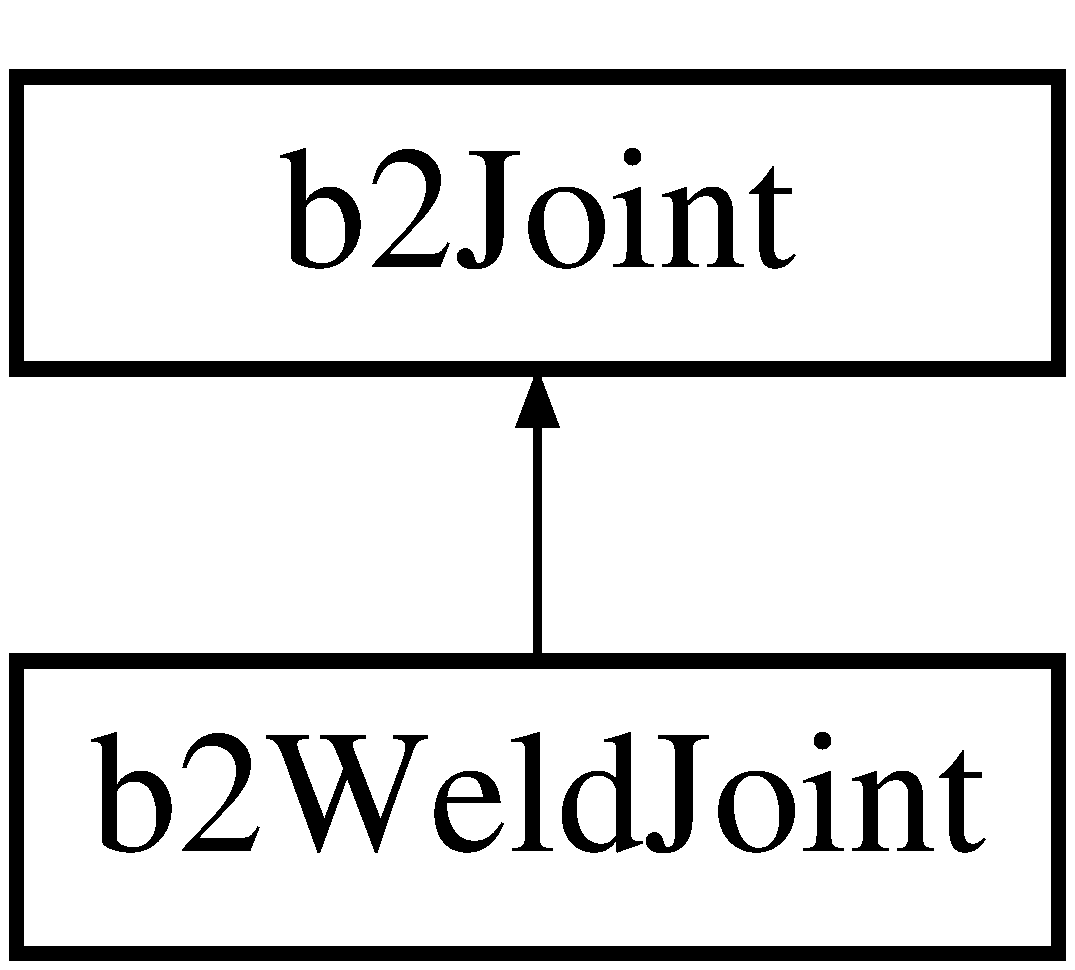
\includegraphics[height=2.000000cm]{classb2WeldJoint}
\end{center}
\end{figure}
\subsection*{Public Member Functions}
\begin{DoxyCompactItemize}
\item 
\mbox{\Hypertarget{classb2WeldJoint_ac675d0b09a4d9567d85bcba8821785bc}\label{classb2WeldJoint_ac675d0b09a4d9567d85bcba8821785bc}} 
\mbox{\hyperlink{structb2Vec2}{b2\+Vec2}} \mbox{\hyperlink{classb2WeldJoint_ac675d0b09a4d9567d85bcba8821785bc}{Get\+AnchorA}} () const override
\begin{DoxyCompactList}\small\item\em Get the anchor point on bodyA in world coordinates. \end{DoxyCompactList}\item 
\mbox{\Hypertarget{classb2WeldJoint_ac97596e42af760d0a035b15213d3341a}\label{classb2WeldJoint_ac97596e42af760d0a035b15213d3341a}} 
\mbox{\hyperlink{structb2Vec2}{b2\+Vec2}} \mbox{\hyperlink{classb2WeldJoint_ac97596e42af760d0a035b15213d3341a}{Get\+AnchorB}} () const override
\begin{DoxyCompactList}\small\item\em Get the anchor point on bodyB in world coordinates. \end{DoxyCompactList}\item 
\mbox{\Hypertarget{classb2WeldJoint_ae5a6e89a36fc7fec7aae528ec2895308}\label{classb2WeldJoint_ae5a6e89a36fc7fec7aae528ec2895308}} 
\mbox{\hyperlink{structb2Vec2}{b2\+Vec2}} \mbox{\hyperlink{classb2WeldJoint_ae5a6e89a36fc7fec7aae528ec2895308}{Get\+Reaction\+Force}} (float32 inv\+\_\+dt) const override
\begin{DoxyCompactList}\small\item\em Get the reaction force on bodyB at the joint anchor in Newtons. \end{DoxyCompactList}\item 
\mbox{\Hypertarget{classb2WeldJoint_aa591fa3cb8238eefa2b39cb7422ff07c}\label{classb2WeldJoint_aa591fa3cb8238eefa2b39cb7422ff07c}} 
float32 \mbox{\hyperlink{classb2WeldJoint_aa591fa3cb8238eefa2b39cb7422ff07c}{Get\+Reaction\+Torque}} (float32 inv\+\_\+dt) const override
\begin{DoxyCompactList}\small\item\em Get the reaction torque on bodyB in N$\ast$m. \end{DoxyCompactList}\item 
\mbox{\Hypertarget{classb2WeldJoint_af3a42eee31a74fe895b07fa694dc4ae5}\label{classb2WeldJoint_af3a42eee31a74fe895b07fa694dc4ae5}} 
const \mbox{\hyperlink{structb2Vec2}{b2\+Vec2}} \& \mbox{\hyperlink{classb2WeldJoint_af3a42eee31a74fe895b07fa694dc4ae5}{Get\+Local\+AnchorA}} () const
\begin{DoxyCompactList}\small\item\em The local anchor point relative to bodyA\textquotesingle{}s origin. \end{DoxyCompactList}\item 
\mbox{\Hypertarget{classb2WeldJoint_ac0c5e6a53b120f0302d2c6d267d40147}\label{classb2WeldJoint_ac0c5e6a53b120f0302d2c6d267d40147}} 
const \mbox{\hyperlink{structb2Vec2}{b2\+Vec2}} \& \mbox{\hyperlink{classb2WeldJoint_ac0c5e6a53b120f0302d2c6d267d40147}{Get\+Local\+AnchorB}} () const
\begin{DoxyCompactList}\small\item\em The local anchor point relative to bodyB\textquotesingle{}s origin. \end{DoxyCompactList}\item 
\mbox{\Hypertarget{classb2WeldJoint_a2be9f207be5b00b775a7576e16d442ef}\label{classb2WeldJoint_a2be9f207be5b00b775a7576e16d442ef}} 
float32 \mbox{\hyperlink{classb2WeldJoint_a2be9f207be5b00b775a7576e16d442ef}{Get\+Reference\+Angle}} () const
\begin{DoxyCompactList}\small\item\em Get the reference angle. \end{DoxyCompactList}\item 
\mbox{\Hypertarget{classb2WeldJoint_a0796404379b7562f1af557729085c447}\label{classb2WeldJoint_a0796404379b7562f1af557729085c447}} 
void \mbox{\hyperlink{classb2WeldJoint_a0796404379b7562f1af557729085c447}{Set\+Frequency}} (float32 hz)
\begin{DoxyCompactList}\small\item\em Set/get frequency in Hz. \end{DoxyCompactList}\item 
\mbox{\Hypertarget{classb2WeldJoint_a36bf80c1c59e28976e286d9ed750b0df}\label{classb2WeldJoint_a36bf80c1c59e28976e286d9ed750b0df}} 
float32 {\bfseries Get\+Frequency} () const
\item 
\mbox{\Hypertarget{classb2WeldJoint_aea79865e590edba09eff9d2243689967}\label{classb2WeldJoint_aea79865e590edba09eff9d2243689967}} 
void \mbox{\hyperlink{classb2WeldJoint_aea79865e590edba09eff9d2243689967}{Set\+Damping\+Ratio}} (float32 ratio)
\begin{DoxyCompactList}\small\item\em Set/get damping ratio. \end{DoxyCompactList}\item 
\mbox{\Hypertarget{classb2WeldJoint_a603d83491d474156b2c09b59a23bfca4}\label{classb2WeldJoint_a603d83491d474156b2c09b59a23bfca4}} 
float32 {\bfseries Get\+Damping\+Ratio} () const
\item 
\mbox{\Hypertarget{classb2WeldJoint_a59de1cad3229b41886bc23c4d6216e2f}\label{classb2WeldJoint_a59de1cad3229b41886bc23c4d6216e2f}} 
void \mbox{\hyperlink{classb2WeldJoint_a59de1cad3229b41886bc23c4d6216e2f}{Dump}} () override
\begin{DoxyCompactList}\small\item\em Dump to b2\+Log. \end{DoxyCompactList}\end{DoxyCompactItemize}
\subsection*{Protected Member Functions}
\begin{DoxyCompactItemize}
\item 
\mbox{\Hypertarget{classb2WeldJoint_a84dbb52e983d9039eab6ad64ae62d8eb}\label{classb2WeldJoint_a84dbb52e983d9039eab6ad64ae62d8eb}} 
{\bfseries b2\+Weld\+Joint} (const \mbox{\hyperlink{structb2WeldJointDef}{b2\+Weld\+Joint\+Def}} $\ast$def)
\item 
\mbox{\Hypertarget{classb2WeldJoint_afb54f848fe19f33555f01594e3e4f410}\label{classb2WeldJoint_afb54f848fe19f33555f01594e3e4f410}} 
void {\bfseries Init\+Velocity\+Constraints} (const \mbox{\hyperlink{structb2SolverData}{b2\+Solver\+Data}} \&data) override
\item 
\mbox{\Hypertarget{classb2WeldJoint_a0367580735b117dcf9a4292df4daf883}\label{classb2WeldJoint_a0367580735b117dcf9a4292df4daf883}} 
void {\bfseries Solve\+Velocity\+Constraints} (const \mbox{\hyperlink{structb2SolverData}{b2\+Solver\+Data}} \&data) override
\item 
\mbox{\Hypertarget{classb2WeldJoint_a068ae45ce6577e27669121032c277015}\label{classb2WeldJoint_a068ae45ce6577e27669121032c277015}} 
bool {\bfseries Solve\+Position\+Constraints} (const \mbox{\hyperlink{structb2SolverData}{b2\+Solver\+Data}} \&data) override
\end{DoxyCompactItemize}
\subsection*{Protected Attributes}
\begin{DoxyCompactItemize}
\item 
\mbox{\Hypertarget{classb2WeldJoint_aa3cd6f08f509f67ad068d0ded7df9f21}\label{classb2WeldJoint_aa3cd6f08f509f67ad068d0ded7df9f21}} 
float32 {\bfseries m\+\_\+frequency\+Hz}
\item 
\mbox{\Hypertarget{classb2WeldJoint_a4a730af358f79a6ccd7641e198eb5c7b}\label{classb2WeldJoint_a4a730af358f79a6ccd7641e198eb5c7b}} 
float32 {\bfseries m\+\_\+damping\+Ratio}
\item 
\mbox{\Hypertarget{classb2WeldJoint_af54a943c1476e6a7c7bcfdf6cf568ba3}\label{classb2WeldJoint_af54a943c1476e6a7c7bcfdf6cf568ba3}} 
float32 {\bfseries m\+\_\+bias}
\item 
\mbox{\Hypertarget{classb2WeldJoint_a572689c5f8c3df6902d64c56a2bb88f2}\label{classb2WeldJoint_a572689c5f8c3df6902d64c56a2bb88f2}} 
\mbox{\hyperlink{structb2Vec2}{b2\+Vec2}} {\bfseries m\+\_\+local\+AnchorA}
\item 
\mbox{\Hypertarget{classb2WeldJoint_a39854cb14c83f88ec65d232b08e70704}\label{classb2WeldJoint_a39854cb14c83f88ec65d232b08e70704}} 
\mbox{\hyperlink{structb2Vec2}{b2\+Vec2}} {\bfseries m\+\_\+local\+AnchorB}
\item 
\mbox{\Hypertarget{classb2WeldJoint_a77639b3636192d6ac7083b33394ae943}\label{classb2WeldJoint_a77639b3636192d6ac7083b33394ae943}} 
float32 {\bfseries m\+\_\+reference\+Angle}
\item 
\mbox{\Hypertarget{classb2WeldJoint_a29a8fc5e8efa796f7a7b439b4978f716}\label{classb2WeldJoint_a29a8fc5e8efa796f7a7b439b4978f716}} 
float32 {\bfseries m\+\_\+gamma}
\item 
\mbox{\Hypertarget{classb2WeldJoint_a47db737b0d94628e7839718cf91cf762}\label{classb2WeldJoint_a47db737b0d94628e7839718cf91cf762}} 
\mbox{\hyperlink{structb2Vec3}{b2\+Vec3}} {\bfseries m\+\_\+impulse}
\item 
\mbox{\Hypertarget{classb2WeldJoint_a4a3aa65b0a4669478db292f6765b03dd}\label{classb2WeldJoint_a4a3aa65b0a4669478db292f6765b03dd}} 
int32 {\bfseries m\+\_\+indexA}
\item 
\mbox{\Hypertarget{classb2WeldJoint_a6e2aa1c13e8c96d9bbbdc6aae6b8e342}\label{classb2WeldJoint_a6e2aa1c13e8c96d9bbbdc6aae6b8e342}} 
int32 {\bfseries m\+\_\+indexB}
\item 
\mbox{\Hypertarget{classb2WeldJoint_abfbbe893b469c6855b297bdd768ba6fe}\label{classb2WeldJoint_abfbbe893b469c6855b297bdd768ba6fe}} 
\mbox{\hyperlink{structb2Vec2}{b2\+Vec2}} {\bfseries m\+\_\+rA}
\item 
\mbox{\Hypertarget{classb2WeldJoint_a2a2af228eb5c2cd38e8baf77098cc3b0}\label{classb2WeldJoint_a2a2af228eb5c2cd38e8baf77098cc3b0}} 
\mbox{\hyperlink{structb2Vec2}{b2\+Vec2}} {\bfseries m\+\_\+rB}
\item 
\mbox{\Hypertarget{classb2WeldJoint_a18360f1e82a3a4e4fdfb3e6cba85160c}\label{classb2WeldJoint_a18360f1e82a3a4e4fdfb3e6cba85160c}} 
\mbox{\hyperlink{structb2Vec2}{b2\+Vec2}} {\bfseries m\+\_\+local\+CenterA}
\item 
\mbox{\Hypertarget{classb2WeldJoint_a71281fbd18892e3f9653490bf85a844a}\label{classb2WeldJoint_a71281fbd18892e3f9653490bf85a844a}} 
\mbox{\hyperlink{structb2Vec2}{b2\+Vec2}} {\bfseries m\+\_\+local\+CenterB}
\item 
\mbox{\Hypertarget{classb2WeldJoint_abb8cd34e03146dbae6af123ed75c2ee5}\label{classb2WeldJoint_abb8cd34e03146dbae6af123ed75c2ee5}} 
float32 {\bfseries m\+\_\+inv\+MassA}
\item 
\mbox{\Hypertarget{classb2WeldJoint_a071f8b347a1167adb144a575749b6fc5}\label{classb2WeldJoint_a071f8b347a1167adb144a575749b6fc5}} 
float32 {\bfseries m\+\_\+inv\+MassB}
\item 
\mbox{\Hypertarget{classb2WeldJoint_af1420cccbd68021c24cc279bf55fabb9}\label{classb2WeldJoint_af1420cccbd68021c24cc279bf55fabb9}} 
float32 {\bfseries m\+\_\+inv\+IA}
\item 
\mbox{\Hypertarget{classb2WeldJoint_a25dc4f3e300ee00a29ca141ac6d894fa}\label{classb2WeldJoint_a25dc4f3e300ee00a29ca141ac6d894fa}} 
float32 {\bfseries m\+\_\+inv\+IB}
\item 
\mbox{\Hypertarget{classb2WeldJoint_ad07c6f68bd3ee2d62e4a8d656d526cf3}\label{classb2WeldJoint_ad07c6f68bd3ee2d62e4a8d656d526cf3}} 
\mbox{\hyperlink{structb2Mat33}{b2\+Mat33}} {\bfseries m\+\_\+mass}
\end{DoxyCompactItemize}
\subsection*{Friends}
\begin{DoxyCompactItemize}
\item 
\mbox{\Hypertarget{classb2WeldJoint_a54ade8ed3d794298108d7f4c4e4793fa}\label{classb2WeldJoint_a54ade8ed3d794298108d7f4c4e4793fa}} 
class {\bfseries b2\+Joint}
\end{DoxyCompactItemize}
\subsection*{Additional Inherited Members}


\subsection{Detailed Description}
A weld joint essentially glues two bodies together. A weld joint may distort somewhat because the island constraint solver is approximate. 

The documentation for this class was generated from the following files\+:\begin{DoxyCompactItemize}
\item 
Dynamics/\+Joints/b2\+Weld\+Joint.\+h\item 
Dynamics/\+Joints/b2\+Weld\+Joint.\+cpp\end{DoxyCompactItemize}

\hypertarget{structb2WeldJointDef}{}\section{b2\+Weld\+Joint\+Def Struct Reference}
\label{structb2WeldJointDef}\index{b2\+Weld\+Joint\+Def@{b2\+Weld\+Joint\+Def}}


{\ttfamily \#include $<$b2\+Weld\+Joint.\+h$>$}

Inheritance diagram for b2\+Weld\+Joint\+Def\+:\begin{figure}[H]
\begin{center}
\leavevmode
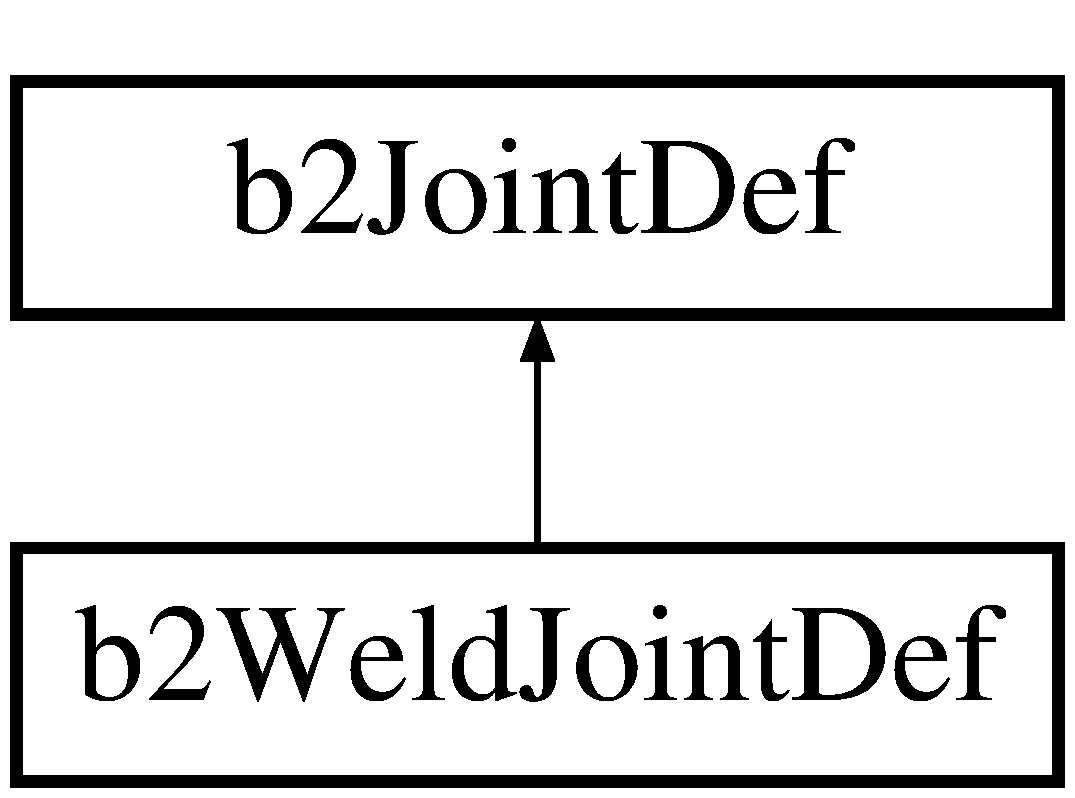
\includegraphics[height=2.000000cm]{structb2WeldJointDef}
\end{center}
\end{figure}
\subsection*{Public Member Functions}
\begin{DoxyCompactItemize}
\item 
void \mbox{\hyperlink{structb2WeldJointDef_a9f6592c2a7eba6ce6e07e40c4e82aab5}{Initialize}} (\mbox{\hyperlink{classb2Body}{b2\+Body}} $\ast$\mbox{\hyperlink{structb2JointDef_a8cd54c93da396be75a9788f2c6897f05}{bodyA}}, \mbox{\hyperlink{classb2Body}{b2\+Body}} $\ast$\mbox{\hyperlink{structb2JointDef_aa4f4dee2fbcd12187b19506b60e68e3d}{bodyB}}, const \mbox{\hyperlink{structb2Vec2}{b2\+Vec2}} \&anchor)
\end{DoxyCompactItemize}
\subsection*{Public Attributes}
\begin{DoxyCompactItemize}
\item 
\mbox{\Hypertarget{structb2WeldJointDef_a3b04af6164bb32efc3f5cf3e8d2b7109}\label{structb2WeldJointDef_a3b04af6164bb32efc3f5cf3e8d2b7109}} 
\mbox{\hyperlink{structb2Vec2}{b2\+Vec2}} \mbox{\hyperlink{structb2WeldJointDef_a3b04af6164bb32efc3f5cf3e8d2b7109}{local\+AnchorA}}
\begin{DoxyCompactList}\small\item\em The local anchor point relative to bodyA\textquotesingle{}s origin. \end{DoxyCompactList}\item 
\mbox{\Hypertarget{structb2WeldJointDef_a528262b92dac10de37411ad8c5637149}\label{structb2WeldJointDef_a528262b92dac10de37411ad8c5637149}} 
\mbox{\hyperlink{structb2Vec2}{b2\+Vec2}} \mbox{\hyperlink{structb2WeldJointDef_a528262b92dac10de37411ad8c5637149}{local\+AnchorB}}
\begin{DoxyCompactList}\small\item\em The local anchor point relative to bodyB\textquotesingle{}s origin. \end{DoxyCompactList}\item 
\mbox{\Hypertarget{structb2WeldJointDef_a31aeb208f15842091c55e3f1bab6d8f1}\label{structb2WeldJointDef_a31aeb208f15842091c55e3f1bab6d8f1}} 
float32 \mbox{\hyperlink{structb2WeldJointDef_a31aeb208f15842091c55e3f1bab6d8f1}{reference\+Angle}}
\begin{DoxyCompactList}\small\item\em The bodyB angle minus bodyA angle in the reference state (radians). \end{DoxyCompactList}\item 
float32 \mbox{\hyperlink{structb2WeldJointDef_abf42ce852914af845e9203b341f55c87}{frequency\+Hz}}
\item 
\mbox{\Hypertarget{structb2WeldJointDef_ace1f0131610f14558f3dbaaed7b10e24}\label{structb2WeldJointDef_ace1f0131610f14558f3dbaaed7b10e24}} 
float32 \mbox{\hyperlink{structb2WeldJointDef_ace1f0131610f14558f3dbaaed7b10e24}{damping\+Ratio}}
\begin{DoxyCompactList}\small\item\em The damping ratio. 0 = no damping, 1 = critical damping. \end{DoxyCompactList}\end{DoxyCompactItemize}


\subsection{Detailed Description}
Weld joint definition. You need to specify local anchor points where they are attached and the relative body angle. The position of the anchor points is important for computing the reaction torque. 

\subsection{Member Function Documentation}
\mbox{\Hypertarget{structb2WeldJointDef_a9f6592c2a7eba6ce6e07e40c4e82aab5}\label{structb2WeldJointDef_a9f6592c2a7eba6ce6e07e40c4e82aab5}} 
\index{b2\+Weld\+Joint\+Def@{b2\+Weld\+Joint\+Def}!Initialize@{Initialize}}
\index{Initialize@{Initialize}!b2\+Weld\+Joint\+Def@{b2\+Weld\+Joint\+Def}}
\subsubsection{\texorpdfstring{Initialize()}{Initialize()}}
{\footnotesize\ttfamily void b2\+Weld\+Joint\+Def\+::\+Initialize (\begin{DoxyParamCaption}\item[{\mbox{\hyperlink{classb2Body}{b2\+Body}} $\ast$}]{bodyA,  }\item[{\mbox{\hyperlink{classb2Body}{b2\+Body}} $\ast$}]{bodyB,  }\item[{const \mbox{\hyperlink{structb2Vec2}{b2\+Vec2}} \&}]{anchor }\end{DoxyParamCaption})}

Initialize the bodies, anchors, and reference angle using a world anchor point. 

\subsection{Member Data Documentation}
\mbox{\Hypertarget{structb2WeldJointDef_abf42ce852914af845e9203b341f55c87}\label{structb2WeldJointDef_abf42ce852914af845e9203b341f55c87}} 
\index{b2\+Weld\+Joint\+Def@{b2\+Weld\+Joint\+Def}!frequency\+Hz@{frequency\+Hz}}
\index{frequency\+Hz@{frequency\+Hz}!b2\+Weld\+Joint\+Def@{b2\+Weld\+Joint\+Def}}
\subsubsection{\texorpdfstring{frequency\+Hz}{frequencyHz}}
{\footnotesize\ttfamily float32 b2\+Weld\+Joint\+Def\+::frequency\+Hz}

The mass-\/spring-\/damper frequency in Hertz. Rotation only. Disable softness with a value of 0. 

The documentation for this struct was generated from the following files\+:\begin{DoxyCompactItemize}
\item 
Dynamics/\+Joints/b2\+Weld\+Joint.\+h\item 
Dynamics/\+Joints/b2\+Weld\+Joint.\+cpp\end{DoxyCompactItemize}

\hypertarget{classb2WheelJoint}{}\section{b2\+Wheel\+Joint Class Reference}
\label{classb2WheelJoint}\index{b2\+Wheel\+Joint@{b2\+Wheel\+Joint}}


{\ttfamily \#include $<$b2\+Wheel\+Joint.\+h$>$}

Inheritance diagram for b2\+Wheel\+Joint\+:\begin{figure}[H]
\begin{center}
\leavevmode
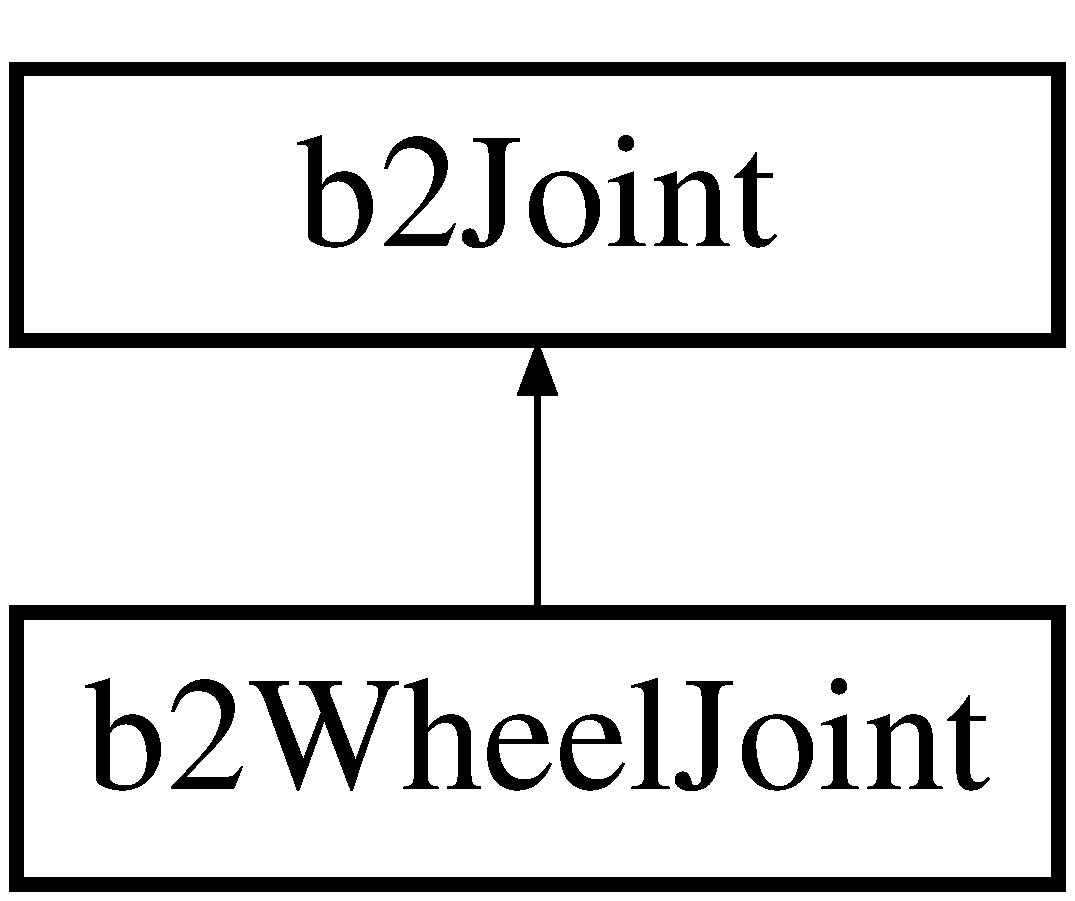
\includegraphics[height=2.000000cm]{classb2WheelJoint}
\end{center}
\end{figure}
\subsection*{Public Member Functions}
\begin{DoxyCompactItemize}
\item 
\mbox{\Hypertarget{classb2WheelJoint_a43a301e48ba486278932c82d3a98abd8}\label{classb2WheelJoint_a43a301e48ba486278932c82d3a98abd8}} 
\mbox{\hyperlink{structb2Vec2}{b2\+Vec2}} \mbox{\hyperlink{classb2WheelJoint_a43a301e48ba486278932c82d3a98abd8}{Get\+AnchorA}} () const override
\begin{DoxyCompactList}\small\item\em Get the anchor point on bodyA in world coordinates. \end{DoxyCompactList}\item 
\mbox{\Hypertarget{classb2WheelJoint_a62f450ad368793c3cde36404a39775e0}\label{classb2WheelJoint_a62f450ad368793c3cde36404a39775e0}} 
\mbox{\hyperlink{structb2Vec2}{b2\+Vec2}} \mbox{\hyperlink{classb2WheelJoint_a62f450ad368793c3cde36404a39775e0}{Get\+AnchorB}} () const override
\begin{DoxyCompactList}\small\item\em Get the anchor point on bodyB in world coordinates. \end{DoxyCompactList}\item 
\mbox{\Hypertarget{classb2WheelJoint_a93e34e700ce794db1acee07562027b2a}\label{classb2WheelJoint_a93e34e700ce794db1acee07562027b2a}} 
\mbox{\hyperlink{structb2Vec2}{b2\+Vec2}} \mbox{\hyperlink{classb2WheelJoint_a93e34e700ce794db1acee07562027b2a}{Get\+Reaction\+Force}} (float32 inv\+\_\+dt) const override
\begin{DoxyCompactList}\small\item\em Get the reaction force on bodyB at the joint anchor in Newtons. \end{DoxyCompactList}\item 
\mbox{\Hypertarget{classb2WheelJoint_ad3317bb9856b105e4cb34d067316d7a8}\label{classb2WheelJoint_ad3317bb9856b105e4cb34d067316d7a8}} 
float32 \mbox{\hyperlink{classb2WheelJoint_ad3317bb9856b105e4cb34d067316d7a8}{Get\+Reaction\+Torque}} (float32 inv\+\_\+dt) const override
\begin{DoxyCompactList}\small\item\em Get the reaction torque on bodyB in N$\ast$m. \end{DoxyCompactList}\item 
\mbox{\Hypertarget{classb2WheelJoint_aaf132c39227962a0b0788558e7dd6662}\label{classb2WheelJoint_aaf132c39227962a0b0788558e7dd6662}} 
const \mbox{\hyperlink{structb2Vec2}{b2\+Vec2}} \& \mbox{\hyperlink{classb2WheelJoint_aaf132c39227962a0b0788558e7dd6662}{Get\+Local\+AnchorA}} () const
\begin{DoxyCompactList}\small\item\em The local anchor point relative to bodyA\textquotesingle{}s origin. \end{DoxyCompactList}\item 
\mbox{\Hypertarget{classb2WheelJoint_a78c56833f42bfc61998aa5ea8c876f3e}\label{classb2WheelJoint_a78c56833f42bfc61998aa5ea8c876f3e}} 
const \mbox{\hyperlink{structb2Vec2}{b2\+Vec2}} \& \mbox{\hyperlink{classb2WheelJoint_a78c56833f42bfc61998aa5ea8c876f3e}{Get\+Local\+AnchorB}} () const
\begin{DoxyCompactList}\small\item\em The local anchor point relative to bodyB\textquotesingle{}s origin. \end{DoxyCompactList}\item 
\mbox{\Hypertarget{classb2WheelJoint_a86bf4dbf356f9095c05d62313810e602}\label{classb2WheelJoint_a86bf4dbf356f9095c05d62313810e602}} 
const \mbox{\hyperlink{structb2Vec2}{b2\+Vec2}} \& \mbox{\hyperlink{classb2WheelJoint_a86bf4dbf356f9095c05d62313810e602}{Get\+Local\+AxisA}} () const
\begin{DoxyCompactList}\small\item\em The local joint axis relative to bodyA. \end{DoxyCompactList}\item 
\mbox{\Hypertarget{classb2WheelJoint_a4cebb70f659344d5d93c1885d47000e3}\label{classb2WheelJoint_a4cebb70f659344d5d93c1885d47000e3}} 
float32 \mbox{\hyperlink{classb2WheelJoint_a4cebb70f659344d5d93c1885d47000e3}{Get\+Joint\+Translation}} () const
\begin{DoxyCompactList}\small\item\em Get the current joint translation, usually in meters. \end{DoxyCompactList}\item 
\mbox{\Hypertarget{classb2WheelJoint_a3cbdc95c55c9bf5b9f2b46b05fc2a5e5}\label{classb2WheelJoint_a3cbdc95c55c9bf5b9f2b46b05fc2a5e5}} 
float32 \mbox{\hyperlink{classb2WheelJoint_a3cbdc95c55c9bf5b9f2b46b05fc2a5e5}{Get\+Joint\+Linear\+Speed}} () const
\begin{DoxyCompactList}\small\item\em Get the current joint linear speed, usually in meters per second. \end{DoxyCompactList}\item 
\mbox{\Hypertarget{classb2WheelJoint_a3ea115dde9bad34d23fd59068734824a}\label{classb2WheelJoint_a3ea115dde9bad34d23fd59068734824a}} 
float32 \mbox{\hyperlink{classb2WheelJoint_a3ea115dde9bad34d23fd59068734824a}{Get\+Joint\+Angle}} () const
\begin{DoxyCompactList}\small\item\em Get the current joint angle in radians. \end{DoxyCompactList}\item 
\mbox{\Hypertarget{classb2WheelJoint_aaf5a4e3713ceca98c2afda950e67ff9d}\label{classb2WheelJoint_aaf5a4e3713ceca98c2afda950e67ff9d}} 
float32 \mbox{\hyperlink{classb2WheelJoint_aaf5a4e3713ceca98c2afda950e67ff9d}{Get\+Joint\+Angular\+Speed}} () const
\begin{DoxyCompactList}\small\item\em Get the current joint angular speed in radians per second. \end{DoxyCompactList}\item 
\mbox{\Hypertarget{classb2WheelJoint_aef7948a18ec2784397a1d3745824cd78}\label{classb2WheelJoint_aef7948a18ec2784397a1d3745824cd78}} 
bool \mbox{\hyperlink{classb2WheelJoint_aef7948a18ec2784397a1d3745824cd78}{Is\+Motor\+Enabled}} () const
\begin{DoxyCompactList}\small\item\em Is the joint motor enabled? \end{DoxyCompactList}\item 
\mbox{\Hypertarget{classb2WheelJoint_a7a832d814bdda135a78fad41ba671da6}\label{classb2WheelJoint_a7a832d814bdda135a78fad41ba671da6}} 
void \mbox{\hyperlink{classb2WheelJoint_a7a832d814bdda135a78fad41ba671da6}{Enable\+Motor}} (bool flag)
\begin{DoxyCompactList}\small\item\em Enable/disable the joint motor. \end{DoxyCompactList}\item 
\mbox{\Hypertarget{classb2WheelJoint_a6e3255fcf5c82b979ad7e3dc1c089c0b}\label{classb2WheelJoint_a6e3255fcf5c82b979ad7e3dc1c089c0b}} 
void \mbox{\hyperlink{classb2WheelJoint_a6e3255fcf5c82b979ad7e3dc1c089c0b}{Set\+Motor\+Speed}} (float32 speed)
\begin{DoxyCompactList}\small\item\em Set the motor speed, usually in radians per second. \end{DoxyCompactList}\item 
\mbox{\Hypertarget{classb2WheelJoint_a47774ba5dfc1a6a5f15bcc651eea8127}\label{classb2WheelJoint_a47774ba5dfc1a6a5f15bcc651eea8127}} 
float32 \mbox{\hyperlink{classb2WheelJoint_a47774ba5dfc1a6a5f15bcc651eea8127}{Get\+Motor\+Speed}} () const
\begin{DoxyCompactList}\small\item\em Get the motor speed, usually in radians per second. \end{DoxyCompactList}\item 
\mbox{\Hypertarget{classb2WheelJoint_a8aae3cd624ec9d48fc86c325c4595edc}\label{classb2WheelJoint_a8aae3cd624ec9d48fc86c325c4595edc}} 
void \mbox{\hyperlink{classb2WheelJoint_a8aae3cd624ec9d48fc86c325c4595edc}{Set\+Max\+Motor\+Torque}} (float32 torque)
\begin{DoxyCompactList}\small\item\em Set/\+Get the maximum motor force, usually in N-\/m. \end{DoxyCompactList}\item 
\mbox{\Hypertarget{classb2WheelJoint_a8e7dc36e5c59760f2807886d0acd514e}\label{classb2WheelJoint_a8e7dc36e5c59760f2807886d0acd514e}} 
float32 {\bfseries Get\+Max\+Motor\+Torque} () const
\item 
\mbox{\Hypertarget{classb2WheelJoint_a635497eba904925e06fd5316ddec4539}\label{classb2WheelJoint_a635497eba904925e06fd5316ddec4539}} 
float32 \mbox{\hyperlink{classb2WheelJoint_a635497eba904925e06fd5316ddec4539}{Get\+Motor\+Torque}} (float32 inv\+\_\+dt) const
\begin{DoxyCompactList}\small\item\em Get the current motor torque given the inverse time step, usually in N-\/m. \end{DoxyCompactList}\item 
\mbox{\Hypertarget{classb2WheelJoint_af9f8fada5cb30f83aa2fbf486e9d347b}\label{classb2WheelJoint_af9f8fada5cb30f83aa2fbf486e9d347b}} 
void \mbox{\hyperlink{classb2WheelJoint_af9f8fada5cb30f83aa2fbf486e9d347b}{Set\+Spring\+Frequency\+Hz}} (float32 hz)
\begin{DoxyCompactList}\small\item\em Set/\+Get the spring frequency in hertz. Setting the frequency to zero disables the spring. \end{DoxyCompactList}\item 
\mbox{\Hypertarget{classb2WheelJoint_a3a22add79f238b4243407956b031c9f4}\label{classb2WheelJoint_a3a22add79f238b4243407956b031c9f4}} 
float32 {\bfseries Get\+Spring\+Frequency\+Hz} () const
\item 
\mbox{\Hypertarget{classb2WheelJoint_a39b123ac045c8ec93faa65746e6655dc}\label{classb2WheelJoint_a39b123ac045c8ec93faa65746e6655dc}} 
void \mbox{\hyperlink{classb2WheelJoint_a39b123ac045c8ec93faa65746e6655dc}{Set\+Spring\+Damping\+Ratio}} (float32 ratio)
\begin{DoxyCompactList}\small\item\em Set/\+Get the spring damping ratio. \end{DoxyCompactList}\item 
\mbox{\Hypertarget{classb2WheelJoint_a18726ad5af314531f518132d6623bc61}\label{classb2WheelJoint_a18726ad5af314531f518132d6623bc61}} 
float32 {\bfseries Get\+Spring\+Damping\+Ratio} () const
\item 
\mbox{\Hypertarget{classb2WheelJoint_a8295644bd733c28c8c9fa6390a367f3f}\label{classb2WheelJoint_a8295644bd733c28c8c9fa6390a367f3f}} 
void \mbox{\hyperlink{classb2WheelJoint_a8295644bd733c28c8c9fa6390a367f3f}{Dump}} () override
\begin{DoxyCompactList}\small\item\em Dump to b2\+Log. \end{DoxyCompactList}\end{DoxyCompactItemize}
\subsection*{Protected Member Functions}
\begin{DoxyCompactItemize}
\item 
\mbox{\Hypertarget{classb2WheelJoint_a9c8bbb1068ddb46d074fe91802dd6a39}\label{classb2WheelJoint_a9c8bbb1068ddb46d074fe91802dd6a39}} 
{\bfseries b2\+Wheel\+Joint} (const \mbox{\hyperlink{structb2WheelJointDef}{b2\+Wheel\+Joint\+Def}} $\ast$def)
\item 
\mbox{\Hypertarget{classb2WheelJoint_a557c58a58cdf75d5b2c14c7f75a37575}\label{classb2WheelJoint_a557c58a58cdf75d5b2c14c7f75a37575}} 
void {\bfseries Init\+Velocity\+Constraints} (const \mbox{\hyperlink{structb2SolverData}{b2\+Solver\+Data}} \&data) override
\item 
\mbox{\Hypertarget{classb2WheelJoint_afbda202bc67d58cac38e3c5b138b93f7}\label{classb2WheelJoint_afbda202bc67d58cac38e3c5b138b93f7}} 
void {\bfseries Solve\+Velocity\+Constraints} (const \mbox{\hyperlink{structb2SolverData}{b2\+Solver\+Data}} \&data) override
\item 
\mbox{\Hypertarget{classb2WheelJoint_addbe70ee831954312bc31dee1d52311f}\label{classb2WheelJoint_addbe70ee831954312bc31dee1d52311f}} 
bool {\bfseries Solve\+Position\+Constraints} (const \mbox{\hyperlink{structb2SolverData}{b2\+Solver\+Data}} \&data) override
\end{DoxyCompactItemize}
\subsection*{Protected Attributes}
\begin{DoxyCompactItemize}
\item 
\mbox{\Hypertarget{classb2WheelJoint_a0570ebb1228c2baca4630c53b77792fa}\label{classb2WheelJoint_a0570ebb1228c2baca4630c53b77792fa}} 
float32 {\bfseries m\+\_\+frequency\+Hz}
\item 
\mbox{\Hypertarget{classb2WheelJoint_a712554f6a298cf8a69bbf546fa465843}\label{classb2WheelJoint_a712554f6a298cf8a69bbf546fa465843}} 
float32 {\bfseries m\+\_\+damping\+Ratio}
\item 
\mbox{\Hypertarget{classb2WheelJoint_a9911353143312dc352928a80c63813c8}\label{classb2WheelJoint_a9911353143312dc352928a80c63813c8}} 
\mbox{\hyperlink{structb2Vec2}{b2\+Vec2}} {\bfseries m\+\_\+local\+AnchorA}
\item 
\mbox{\Hypertarget{classb2WheelJoint_a1bc3fa1a0bad5eb2cc7b9962976c1d29}\label{classb2WheelJoint_a1bc3fa1a0bad5eb2cc7b9962976c1d29}} 
\mbox{\hyperlink{structb2Vec2}{b2\+Vec2}} {\bfseries m\+\_\+local\+AnchorB}
\item 
\mbox{\Hypertarget{classb2WheelJoint_ae1cadd777bdffbb726b15c438e081c21}\label{classb2WheelJoint_ae1cadd777bdffbb726b15c438e081c21}} 
\mbox{\hyperlink{structb2Vec2}{b2\+Vec2}} {\bfseries m\+\_\+local\+X\+AxisA}
\item 
\mbox{\Hypertarget{classb2WheelJoint_a5e9566b969c24428d32ff2069d4180e3}\label{classb2WheelJoint_a5e9566b969c24428d32ff2069d4180e3}} 
\mbox{\hyperlink{structb2Vec2}{b2\+Vec2}} {\bfseries m\+\_\+local\+Y\+AxisA}
\item 
\mbox{\Hypertarget{classb2WheelJoint_a81a874642cc60caa2eb212eda3b266f0}\label{classb2WheelJoint_a81a874642cc60caa2eb212eda3b266f0}} 
float32 {\bfseries m\+\_\+impulse}
\item 
\mbox{\Hypertarget{classb2WheelJoint_a1116db6834e3b62a651558f6bdfe000e}\label{classb2WheelJoint_a1116db6834e3b62a651558f6bdfe000e}} 
float32 {\bfseries m\+\_\+motor\+Impulse}
\item 
\mbox{\Hypertarget{classb2WheelJoint_a83aa86813105dc1189fed8acf1767eb5}\label{classb2WheelJoint_a83aa86813105dc1189fed8acf1767eb5}} 
float32 {\bfseries m\+\_\+spring\+Impulse}
\item 
\mbox{\Hypertarget{classb2WheelJoint_ad671dcec7ecd41baf87200b2f9c37c34}\label{classb2WheelJoint_ad671dcec7ecd41baf87200b2f9c37c34}} 
float32 {\bfseries m\+\_\+max\+Motor\+Torque}
\item 
\mbox{\Hypertarget{classb2WheelJoint_a29194860b36867eb4349eee73e8d5908}\label{classb2WheelJoint_a29194860b36867eb4349eee73e8d5908}} 
float32 {\bfseries m\+\_\+motor\+Speed}
\item 
\mbox{\Hypertarget{classb2WheelJoint_a46dae5c1e2630430ce7cf00dbccee8a1}\label{classb2WheelJoint_a46dae5c1e2630430ce7cf00dbccee8a1}} 
bool {\bfseries m\+\_\+enable\+Motor}
\item 
\mbox{\Hypertarget{classb2WheelJoint_a0924e1788c097b3b05eac9cd53d1d997}\label{classb2WheelJoint_a0924e1788c097b3b05eac9cd53d1d997}} 
int32 {\bfseries m\+\_\+indexA}
\item 
\mbox{\Hypertarget{classb2WheelJoint_a76d74ec2f2bf7c941076c0e224c2a9e9}\label{classb2WheelJoint_a76d74ec2f2bf7c941076c0e224c2a9e9}} 
int32 {\bfseries m\+\_\+indexB}
\item 
\mbox{\Hypertarget{classb2WheelJoint_a60c54ed81993fd710b9499f2d6bcc274}\label{classb2WheelJoint_a60c54ed81993fd710b9499f2d6bcc274}} 
\mbox{\hyperlink{structb2Vec2}{b2\+Vec2}} {\bfseries m\+\_\+local\+CenterA}
\item 
\mbox{\Hypertarget{classb2WheelJoint_a7631ce1cbb3b7f33d304eb87a5413277}\label{classb2WheelJoint_a7631ce1cbb3b7f33d304eb87a5413277}} 
\mbox{\hyperlink{structb2Vec2}{b2\+Vec2}} {\bfseries m\+\_\+local\+CenterB}
\item 
\mbox{\Hypertarget{classb2WheelJoint_affa854f7bdde3468b46f416836791192}\label{classb2WheelJoint_affa854f7bdde3468b46f416836791192}} 
float32 {\bfseries m\+\_\+inv\+MassA}
\item 
\mbox{\Hypertarget{classb2WheelJoint_a8ca9663e91d3dd86bdb537248f09c5c7}\label{classb2WheelJoint_a8ca9663e91d3dd86bdb537248f09c5c7}} 
float32 {\bfseries m\+\_\+inv\+MassB}
\item 
\mbox{\Hypertarget{classb2WheelJoint_aa540d2ad4452012952fd42941eefa7d9}\label{classb2WheelJoint_aa540d2ad4452012952fd42941eefa7d9}} 
float32 {\bfseries m\+\_\+inv\+IA}
\item 
\mbox{\Hypertarget{classb2WheelJoint_a6b76c82b51bdf6910d6c241146b1a696}\label{classb2WheelJoint_a6b76c82b51bdf6910d6c241146b1a696}} 
float32 {\bfseries m\+\_\+inv\+IB}
\item 
\mbox{\Hypertarget{classb2WheelJoint_ae91286452d1941d4bed387bd7ee187c8}\label{classb2WheelJoint_ae91286452d1941d4bed387bd7ee187c8}} 
\mbox{\hyperlink{structb2Vec2}{b2\+Vec2}} {\bfseries m\+\_\+ax}
\item 
\mbox{\Hypertarget{classb2WheelJoint_a2f3b7d45948c68e5c5dd8636ed8a8db1}\label{classb2WheelJoint_a2f3b7d45948c68e5c5dd8636ed8a8db1}} 
\mbox{\hyperlink{structb2Vec2}{b2\+Vec2}} {\bfseries m\+\_\+ay}
\item 
\mbox{\Hypertarget{classb2WheelJoint_a0935bcd6aea2145f6c8e947159a1e59b}\label{classb2WheelJoint_a0935bcd6aea2145f6c8e947159a1e59b}} 
float32 {\bfseries m\+\_\+s\+Ax}
\item 
\mbox{\Hypertarget{classb2WheelJoint_a0705a4e0dfd40bf25f518bb22d6e0177}\label{classb2WheelJoint_a0705a4e0dfd40bf25f518bb22d6e0177}} 
float32 {\bfseries m\+\_\+s\+Bx}
\item 
\mbox{\Hypertarget{classb2WheelJoint_aaeb83f256ec67556cc1d7758f75b773e}\label{classb2WheelJoint_aaeb83f256ec67556cc1d7758f75b773e}} 
float32 {\bfseries m\+\_\+s\+Ay}
\item 
\mbox{\Hypertarget{classb2WheelJoint_a4fa320609b2942eee344ac0d91003444}\label{classb2WheelJoint_a4fa320609b2942eee344ac0d91003444}} 
float32 {\bfseries m\+\_\+s\+By}
\item 
\mbox{\Hypertarget{classb2WheelJoint_a80abc7c0fe5a4d6f362ec5cb13214ec1}\label{classb2WheelJoint_a80abc7c0fe5a4d6f362ec5cb13214ec1}} 
float32 {\bfseries m\+\_\+mass}
\item 
\mbox{\Hypertarget{classb2WheelJoint_a64d20e079b2638995c7faa5d3a2aed68}\label{classb2WheelJoint_a64d20e079b2638995c7faa5d3a2aed68}} 
float32 {\bfseries m\+\_\+motor\+Mass}
\item 
\mbox{\Hypertarget{classb2WheelJoint_ab24b6e3ad48961de7d78e4476531dd30}\label{classb2WheelJoint_ab24b6e3ad48961de7d78e4476531dd30}} 
float32 {\bfseries m\+\_\+spring\+Mass}
\item 
\mbox{\Hypertarget{classb2WheelJoint_a82bec93fb4a2a3702455bede3d5c6ac8}\label{classb2WheelJoint_a82bec93fb4a2a3702455bede3d5c6ac8}} 
float32 {\bfseries m\+\_\+bias}
\item 
\mbox{\Hypertarget{classb2WheelJoint_a3d4c8b3e96b517d13693285e63a917fb}\label{classb2WheelJoint_a3d4c8b3e96b517d13693285e63a917fb}} 
float32 {\bfseries m\+\_\+gamma}
\end{DoxyCompactItemize}
\subsection*{Friends}
\begin{DoxyCompactItemize}
\item 
\mbox{\Hypertarget{classb2WheelJoint_a54ade8ed3d794298108d7f4c4e4793fa}\label{classb2WheelJoint_a54ade8ed3d794298108d7f4c4e4793fa}} 
class {\bfseries b2\+Joint}
\end{DoxyCompactItemize}
\subsection*{Additional Inherited Members}


\subsection{Detailed Description}
A wheel joint. This joint provides two degrees of freedom\+: translation along an axis fixed in bodyA and rotation in the plane. In other words, it is a point to line constraint with a rotational motor and a linear spring/damper. This joint is designed for vehicle suspensions. 

The documentation for this class was generated from the following files\+:\begin{DoxyCompactItemize}
\item 
Dynamics/\+Joints/b2\+Wheel\+Joint.\+h\item 
Dynamics/\+Joints/b2\+Wheel\+Joint.\+cpp\end{DoxyCompactItemize}

\hypertarget{structb2WheelJointDef}{}\section{b2\+Wheel\+Joint\+Def Struct Reference}
\label{structb2WheelJointDef}\index{b2\+Wheel\+Joint\+Def@{b2\+Wheel\+Joint\+Def}}


{\ttfamily \#include $<$b2\+Wheel\+Joint.\+h$>$}

Inheritance diagram for b2\+Wheel\+Joint\+Def\+:\begin{figure}[H]
\begin{center}
\leavevmode
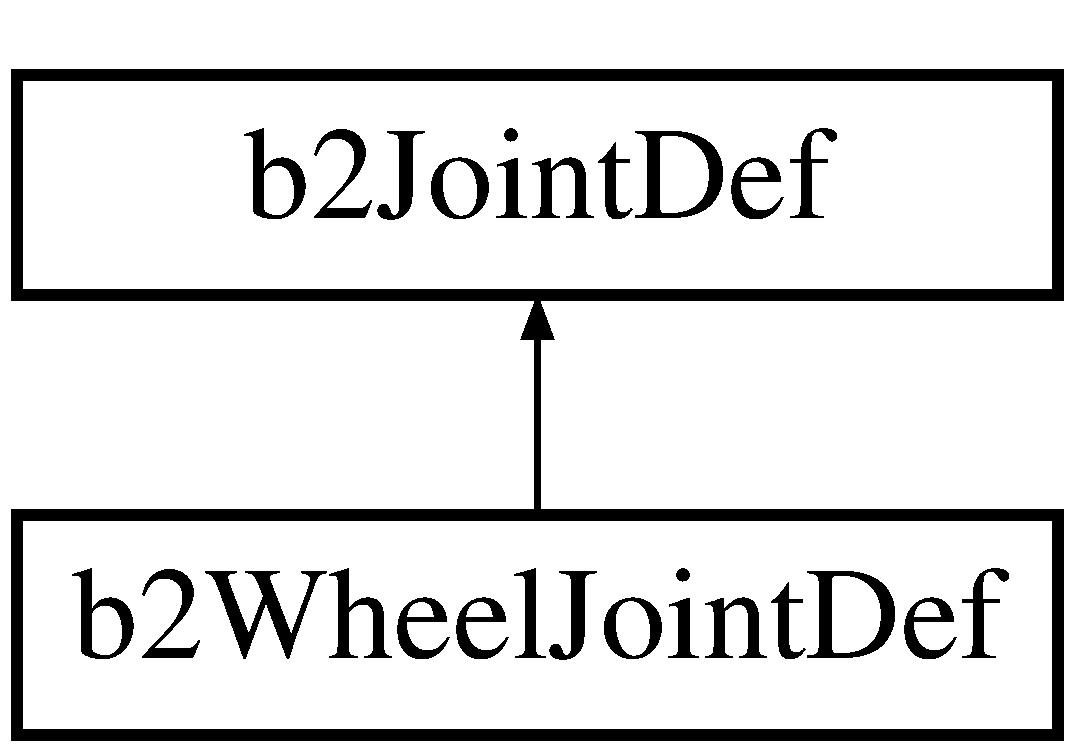
\includegraphics[height=2.000000cm]{structb2WheelJointDef}
\end{center}
\end{figure}
\subsection*{Public Member Functions}
\begin{DoxyCompactItemize}
\item 
void \mbox{\hyperlink{structb2WheelJointDef_af26887092d36c3cd03898401a38783e2}{Initialize}} (\mbox{\hyperlink{classb2Body}{b2\+Body}} $\ast$\mbox{\hyperlink{structb2JointDef_a8cd54c93da396be75a9788f2c6897f05}{bodyA}}, \mbox{\hyperlink{classb2Body}{b2\+Body}} $\ast$\mbox{\hyperlink{structb2JointDef_aa4f4dee2fbcd12187b19506b60e68e3d}{bodyB}}, const \mbox{\hyperlink{structb2Vec2}{b2\+Vec2}} \&anchor, const \mbox{\hyperlink{structb2Vec2}{b2\+Vec2}} \&axis)
\end{DoxyCompactItemize}
\subsection*{Public Attributes}
\begin{DoxyCompactItemize}
\item 
\mbox{\Hypertarget{structb2WheelJointDef_a9429d2273bfdd8bdc0db416e73b89ae4}\label{structb2WheelJointDef_a9429d2273bfdd8bdc0db416e73b89ae4}} 
\mbox{\hyperlink{structb2Vec2}{b2\+Vec2}} \mbox{\hyperlink{structb2WheelJointDef_a9429d2273bfdd8bdc0db416e73b89ae4}{local\+AnchorA}}
\begin{DoxyCompactList}\small\item\em The local anchor point relative to bodyA\textquotesingle{}s origin. \end{DoxyCompactList}\item 
\mbox{\Hypertarget{structb2WheelJointDef_a88ba0f7108076b9d7ced68425be95c27}\label{structb2WheelJointDef_a88ba0f7108076b9d7ced68425be95c27}} 
\mbox{\hyperlink{structb2Vec2}{b2\+Vec2}} \mbox{\hyperlink{structb2WheelJointDef_a88ba0f7108076b9d7ced68425be95c27}{local\+AnchorB}}
\begin{DoxyCompactList}\small\item\em The local anchor point relative to bodyB\textquotesingle{}s origin. \end{DoxyCompactList}\item 
\mbox{\Hypertarget{structb2WheelJointDef_ad635ee7b77b50037dc0e021a0f5c93a6}\label{structb2WheelJointDef_ad635ee7b77b50037dc0e021a0f5c93a6}} 
\mbox{\hyperlink{structb2Vec2}{b2\+Vec2}} \mbox{\hyperlink{structb2WheelJointDef_ad635ee7b77b50037dc0e021a0f5c93a6}{local\+AxisA}}
\begin{DoxyCompactList}\small\item\em The local translation axis in bodyA. \end{DoxyCompactList}\item 
\mbox{\Hypertarget{structb2WheelJointDef_a8e7193d6c34c784ffd71e79d3a70acc6}\label{structb2WheelJointDef_a8e7193d6c34c784ffd71e79d3a70acc6}} 
bool \mbox{\hyperlink{structb2WheelJointDef_a8e7193d6c34c784ffd71e79d3a70acc6}{enable\+Motor}}
\begin{DoxyCompactList}\small\item\em Enable/disable the joint motor. \end{DoxyCompactList}\item 
\mbox{\Hypertarget{structb2WheelJointDef_ab658ce0fae40c6de09133659f7ffb829}\label{structb2WheelJointDef_ab658ce0fae40c6de09133659f7ffb829}} 
float32 \mbox{\hyperlink{structb2WheelJointDef_ab658ce0fae40c6de09133659f7ffb829}{max\+Motor\+Torque}}
\begin{DoxyCompactList}\small\item\em The maximum motor torque, usually in N-\/m. \end{DoxyCompactList}\item 
\mbox{\Hypertarget{structb2WheelJointDef_a7248e25f2ca6b6c2a5f7079ce16e7748}\label{structb2WheelJointDef_a7248e25f2ca6b6c2a5f7079ce16e7748}} 
float32 \mbox{\hyperlink{structb2WheelJointDef_a7248e25f2ca6b6c2a5f7079ce16e7748}{motor\+Speed}}
\begin{DoxyCompactList}\small\item\em The desired motor speed in radians per second. \end{DoxyCompactList}\item 
\mbox{\Hypertarget{structb2WheelJointDef_acf3540f46eaf3bc91426386939bd37b1}\label{structb2WheelJointDef_acf3540f46eaf3bc91426386939bd37b1}} 
float32 \mbox{\hyperlink{structb2WheelJointDef_acf3540f46eaf3bc91426386939bd37b1}{frequency\+Hz}}
\begin{DoxyCompactList}\small\item\em Suspension frequency, zero indicates no suspension. \end{DoxyCompactList}\item 
\mbox{\Hypertarget{structb2WheelJointDef_a9976584bfee18b46dec355764797ce54}\label{structb2WheelJointDef_a9976584bfee18b46dec355764797ce54}} 
float32 \mbox{\hyperlink{structb2WheelJointDef_a9976584bfee18b46dec355764797ce54}{damping\+Ratio}}
\begin{DoxyCompactList}\small\item\em Suspension damping ratio, one indicates critical damping. \end{DoxyCompactList}\end{DoxyCompactItemize}


\subsection{Detailed Description}
Wheel joint definition. This requires defining a line of motion using an axis and an anchor point. The definition uses local anchor points and a local axis so that the initial configuration can violate the constraint slightly. The joint translation is zero when the local anchor points coincide in world space. Using local anchors and a local axis helps when saving and loading a game. 

\subsection{Member Function Documentation}
\mbox{\Hypertarget{structb2WheelJointDef_af26887092d36c3cd03898401a38783e2}\label{structb2WheelJointDef_af26887092d36c3cd03898401a38783e2}} 
\index{b2\+Wheel\+Joint\+Def@{b2\+Wheel\+Joint\+Def}!Initialize@{Initialize}}
\index{Initialize@{Initialize}!b2\+Wheel\+Joint\+Def@{b2\+Wheel\+Joint\+Def}}
\subsubsection{\texorpdfstring{Initialize()}{Initialize()}}
{\footnotesize\ttfamily void b2\+Wheel\+Joint\+Def\+::\+Initialize (\begin{DoxyParamCaption}\item[{\mbox{\hyperlink{classb2Body}{b2\+Body}} $\ast$}]{bodyA,  }\item[{\mbox{\hyperlink{classb2Body}{b2\+Body}} $\ast$}]{bodyB,  }\item[{const \mbox{\hyperlink{structb2Vec2}{b2\+Vec2}} \&}]{anchor,  }\item[{const \mbox{\hyperlink{structb2Vec2}{b2\+Vec2}} \&}]{axis }\end{DoxyParamCaption})}

Initialize the bodies, anchors, axis, and reference angle using the world anchor and world axis. 

The documentation for this struct was generated from the following files\+:\begin{DoxyCompactItemize}
\item 
Dynamics/\+Joints/b2\+Wheel\+Joint.\+h\item 
Dynamics/\+Joints/b2\+Wheel\+Joint.\+cpp\end{DoxyCompactItemize}

\hypertarget{classb2World}{}\section{b2\+World Class Reference}
\label{classb2World}\index{b2\+World@{b2\+World}}


{\ttfamily \#include $<$b2\+World.\+h$>$}

\subsection*{Public Member Functions}
\begin{DoxyCompactItemize}
\item 
\mbox{\hyperlink{classb2World_aeccc87fd9e36702c821a8244ca7cd875}{b2\+World}} (const \mbox{\hyperlink{structb2Vec2}{b2\+Vec2}} \&gravity)
\item 
\mbox{\Hypertarget{classb2World_a5250ae4487475c33ccefdead07c768c8}\label{classb2World_a5250ae4487475c33ccefdead07c768c8}} 
\mbox{\hyperlink{classb2World_a5250ae4487475c33ccefdead07c768c8}{$\sim$b2\+World}} ()
\begin{DoxyCompactList}\small\item\em Destruct the world. All physics entities are destroyed and all heap memory is released. \end{DoxyCompactList}\item 
void \mbox{\hyperlink{classb2World_ae377f2dd5512ada7d27f4ad3541c75bf}{Set\+Destruction\+Listener}} (\mbox{\hyperlink{classb2DestructionListener}{b2\+Destruction\+Listener}} $\ast$listener)
\item 
void \mbox{\hyperlink{classb2World_a85e6e1e911c7d6366f8c7d57a12b72ff}{Set\+Contact\+Filter}} (\mbox{\hyperlink{classb2ContactFilter}{b2\+Contact\+Filter}} $\ast$filter)
\item 
void \mbox{\hyperlink{classb2World_a614549967fb8a1584b61c11e2d553d42}{Set\+Contact\+Listener}} (\mbox{\hyperlink{classb2ContactListener}{b2\+Contact\+Listener}} $\ast$listener)
\item 
void \mbox{\hyperlink{classb2World_a6976d2c67400df03c0d44174ffcfb7ee}{Set\+Debug\+Draw}} (\mbox{\hyperlink{classb2Draw}{b2\+Draw}} $\ast$debug\+Draw)
\item 
\mbox{\hyperlink{classb2Body}{b2\+Body}} $\ast$ \mbox{\hyperlink{classb2World_a2eb36e967e43294bfa03ec3d177c2dae}{Create\+Body}} (const \mbox{\hyperlink{structb2BodyDef}{b2\+Body\+Def}} $\ast$def)
\item 
void \mbox{\hyperlink{classb2World_ad52231ad7a9556ef5735ac79cbcd8fcf}{Destroy\+Body}} (\mbox{\hyperlink{classb2Body}{b2\+Body}} $\ast$body)
\item 
\mbox{\hyperlink{classb2Joint}{b2\+Joint}} $\ast$ \mbox{\hyperlink{classb2World_a5cba9d0653149eb62504154e6fb35021}{Create\+Joint}} (const \mbox{\hyperlink{structb2JointDef}{b2\+Joint\+Def}} $\ast$def)
\item 
void \mbox{\hyperlink{classb2World_add5942aef171e54cfa384c8975746dca}{Destroy\+Joint}} (\mbox{\hyperlink{classb2Joint}{b2\+Joint}} $\ast$joint)
\item 
void \mbox{\hyperlink{classb2World_a7a8eff61af98461f978fe43f3af7be90}{Step}} (float32 time\+Step, int32 velocity\+Iterations, int32 position\+Iterations)
\item 
void \mbox{\hyperlink{classb2World_ac082ab4c4ad0b1c5ec4674315eeec643}{Clear\+Forces}} ()
\item 
\mbox{\Hypertarget{classb2World_a293d9865e407fd463e168b0a29856acc}\label{classb2World_a293d9865e407fd463e168b0a29856acc}} 
void \mbox{\hyperlink{classb2World_a293d9865e407fd463e168b0a29856acc}{Draw\+Debug\+Data}} ()
\begin{DoxyCompactList}\small\item\em Call this to draw shapes and other debug draw data. This is intentionally non-\/const. \end{DoxyCompactList}\item 
void \mbox{\hyperlink{classb2World_ad169fae775be1e1f16386f7587786fa8}{Query\+A\+A\+BB}} (\mbox{\hyperlink{classb2QueryCallback}{b2\+Query\+Callback}} $\ast$callback, const \mbox{\hyperlink{structb2AABB}{b2\+A\+A\+BB}} \&aabb) const
\item 
void \mbox{\hyperlink{classb2World_aa9955d94a254253997daaf16ce77bab6}{Ray\+Cast}} (\mbox{\hyperlink{classb2RayCastCallback}{b2\+Ray\+Cast\+Callback}} $\ast$callback, const \mbox{\hyperlink{structb2Vec2}{b2\+Vec2}} \&point1, const \mbox{\hyperlink{structb2Vec2}{b2\+Vec2}} \&point2) const
\item 
\mbox{\hyperlink{classb2Body}{b2\+Body}} $\ast$ \mbox{\hyperlink{classb2World_a1b87c03955e3312d308ddf679adf3c85}{Get\+Body\+List}} ()
\item 
\mbox{\Hypertarget{classb2World_a8afde497a719bb1507fdfb474e79881a}\label{classb2World_a8afde497a719bb1507fdfb474e79881a}} 
const \mbox{\hyperlink{classb2Body}{b2\+Body}} $\ast$ {\bfseries Get\+Body\+List} () const
\item 
\mbox{\hyperlink{classb2Joint}{b2\+Joint}} $\ast$ \mbox{\hyperlink{classb2World_a55db7240f8290aa02cab79f181934de8}{Get\+Joint\+List}} ()
\item 
\mbox{\Hypertarget{classb2World_af5f7feca7396ce10b905966a464177aa}\label{classb2World_af5f7feca7396ce10b905966a464177aa}} 
const \mbox{\hyperlink{classb2Joint}{b2\+Joint}} $\ast$ {\bfseries Get\+Joint\+List} () const
\item 
\mbox{\hyperlink{classb2Contact}{b2\+Contact}} $\ast$ \mbox{\hyperlink{classb2World_ab1e1c59fd7534c0268c2a3e31370a425}{Get\+Contact\+List}} ()
\item 
\mbox{\Hypertarget{classb2World_a8a947dbda196b037b922d62e6a54062f}\label{classb2World_a8a947dbda196b037b922d62e6a54062f}} 
const \mbox{\hyperlink{classb2Contact}{b2\+Contact}} $\ast$ {\bfseries Get\+Contact\+List} () const
\item 
\mbox{\Hypertarget{classb2World_a6755872564fc3db70c69d2b9d349fa33}\label{classb2World_a6755872564fc3db70c69d2b9d349fa33}} 
void \mbox{\hyperlink{classb2World_a6755872564fc3db70c69d2b9d349fa33}{Set\+Allow\+Sleeping}} (bool flag)
\begin{DoxyCompactList}\small\item\em Enable/disable sleep. \end{DoxyCompactList}\item 
\mbox{\Hypertarget{classb2World_a3d7ce9b87a54fb4f84433f6223d81175}\label{classb2World_a3d7ce9b87a54fb4f84433f6223d81175}} 
bool {\bfseries Get\+Allow\+Sleeping} () const
\item 
\mbox{\Hypertarget{classb2World_a8e8c12142e8c4884a18787926a261359}\label{classb2World_a8e8c12142e8c4884a18787926a261359}} 
void \mbox{\hyperlink{classb2World_a8e8c12142e8c4884a18787926a261359}{Set\+Warm\+Starting}} (bool flag)
\begin{DoxyCompactList}\small\item\em Enable/disable warm starting. For testing. \end{DoxyCompactList}\item 
\mbox{\Hypertarget{classb2World_af23e93dbf44ebfc3c7ce9dfdc00b8ff7}\label{classb2World_af23e93dbf44ebfc3c7ce9dfdc00b8ff7}} 
bool {\bfseries Get\+Warm\+Starting} () const
\item 
\mbox{\Hypertarget{classb2World_a536dd9181c2e20096073e3cfe2c8530a}\label{classb2World_a536dd9181c2e20096073e3cfe2c8530a}} 
void \mbox{\hyperlink{classb2World_a536dd9181c2e20096073e3cfe2c8530a}{Set\+Continuous\+Physics}} (bool flag)
\begin{DoxyCompactList}\small\item\em Enable/disable continuous physics. For testing. \end{DoxyCompactList}\item 
\mbox{\Hypertarget{classb2World_afec853cfec7a8bbffc20d4acc99963e7}\label{classb2World_afec853cfec7a8bbffc20d4acc99963e7}} 
bool {\bfseries Get\+Continuous\+Physics} () const
\item 
\mbox{\Hypertarget{classb2World_ae8aacc78ea4753075067daff51b61778}\label{classb2World_ae8aacc78ea4753075067daff51b61778}} 
void \mbox{\hyperlink{classb2World_ae8aacc78ea4753075067daff51b61778}{Set\+Sub\+Stepping}} (bool flag)
\begin{DoxyCompactList}\small\item\em Enable/disable single stepped continuous physics. For testing. \end{DoxyCompactList}\item 
\mbox{\Hypertarget{classb2World_aa41f23e3e12f82ce229ce644ecdac28b}\label{classb2World_aa41f23e3e12f82ce229ce644ecdac28b}} 
bool {\bfseries Get\+Sub\+Stepping} () const
\item 
\mbox{\Hypertarget{classb2World_a088742d580bfc42531790ea8747bb8f8}\label{classb2World_a088742d580bfc42531790ea8747bb8f8}} 
int32 \mbox{\hyperlink{classb2World_a088742d580bfc42531790ea8747bb8f8}{Get\+Proxy\+Count}} () const
\begin{DoxyCompactList}\small\item\em Get the number of broad-\/phase proxies. \end{DoxyCompactList}\item 
\mbox{\Hypertarget{classb2World_a41c8b37baf5165c06932e8f08eb758de}\label{classb2World_a41c8b37baf5165c06932e8f08eb758de}} 
int32 \mbox{\hyperlink{classb2World_a41c8b37baf5165c06932e8f08eb758de}{Get\+Body\+Count}} () const
\begin{DoxyCompactList}\small\item\em Get the number of bodies. \end{DoxyCompactList}\item 
\mbox{\Hypertarget{classb2World_a98bd6ca53dbc376f210beced33901934}\label{classb2World_a98bd6ca53dbc376f210beced33901934}} 
int32 \mbox{\hyperlink{classb2World_a98bd6ca53dbc376f210beced33901934}{Get\+Joint\+Count}} () const
\begin{DoxyCompactList}\small\item\em Get the number of joints. \end{DoxyCompactList}\item 
\mbox{\Hypertarget{classb2World_aa47375fc3ca9f09d0350c61cfeabcee9}\label{classb2World_aa47375fc3ca9f09d0350c61cfeabcee9}} 
int32 \mbox{\hyperlink{classb2World_aa47375fc3ca9f09d0350c61cfeabcee9}{Get\+Contact\+Count}} () const
\begin{DoxyCompactList}\small\item\em Get the number of contacts (each may have 0 or more contact points). \end{DoxyCompactList}\item 
\mbox{\Hypertarget{classb2World_abc99b2beb6ba79ac6c80f33bac264b52}\label{classb2World_abc99b2beb6ba79ac6c80f33bac264b52}} 
int32 \mbox{\hyperlink{classb2World_abc99b2beb6ba79ac6c80f33bac264b52}{Get\+Tree\+Height}} () const
\begin{DoxyCompactList}\small\item\em Get the height of the dynamic tree. \end{DoxyCompactList}\item 
\mbox{\Hypertarget{classb2World_aaca027331f06d93d978b44e065873f80}\label{classb2World_aaca027331f06d93d978b44e065873f80}} 
int32 \mbox{\hyperlink{classb2World_aaca027331f06d93d978b44e065873f80}{Get\+Tree\+Balance}} () const
\begin{DoxyCompactList}\small\item\em Get the balance of the dynamic tree. \end{DoxyCompactList}\item 
float32 \mbox{\hyperlink{classb2World_a562935b3b8161dd18a467e02f479e88a}{Get\+Tree\+Quality}} () const
\item 
\mbox{\Hypertarget{classb2World_aeafa43d6580e1dddb0675e672ca2375c}\label{classb2World_aeafa43d6580e1dddb0675e672ca2375c}} 
void \mbox{\hyperlink{classb2World_aeafa43d6580e1dddb0675e672ca2375c}{Set\+Gravity}} (const \mbox{\hyperlink{structb2Vec2}{b2\+Vec2}} \&gravity)
\begin{DoxyCompactList}\small\item\em Change the global gravity vector. \end{DoxyCompactList}\item 
\mbox{\Hypertarget{classb2World_abd41cdde8eaa3d1c58d2f00eaf688ec3}\label{classb2World_abd41cdde8eaa3d1c58d2f00eaf688ec3}} 
\mbox{\hyperlink{structb2Vec2}{b2\+Vec2}} \mbox{\hyperlink{classb2World_abd41cdde8eaa3d1c58d2f00eaf688ec3}{Get\+Gravity}} () const
\begin{DoxyCompactList}\small\item\em Get the global gravity vector. \end{DoxyCompactList}\item 
\mbox{\Hypertarget{classb2World_a71ca09a3082945a7e77f3f39fb021237}\label{classb2World_a71ca09a3082945a7e77f3f39fb021237}} 
bool \mbox{\hyperlink{classb2World_a71ca09a3082945a7e77f3f39fb021237}{Is\+Locked}} () const
\begin{DoxyCompactList}\small\item\em Is the world locked (in the middle of a time step). \end{DoxyCompactList}\item 
\mbox{\Hypertarget{classb2World_aa2bced28ddef5bbb00ed5666e5e9f620}\label{classb2World_aa2bced28ddef5bbb00ed5666e5e9f620}} 
void \mbox{\hyperlink{classb2World_aa2bced28ddef5bbb00ed5666e5e9f620}{Set\+Auto\+Clear\+Forces}} (bool flag)
\begin{DoxyCompactList}\small\item\em Set flag to control automatic clearing of forces after each time step. \end{DoxyCompactList}\item 
\mbox{\Hypertarget{classb2World_ae1fa8272edf37a4e2a7be08f6e0a8cc6}\label{classb2World_ae1fa8272edf37a4e2a7be08f6e0a8cc6}} 
bool \mbox{\hyperlink{classb2World_ae1fa8272edf37a4e2a7be08f6e0a8cc6}{Get\+Auto\+Clear\+Forces}} () const
\begin{DoxyCompactList}\small\item\em Get the flag that controls automatic clearing of forces after each time step. \end{DoxyCompactList}\item 
void \mbox{\hyperlink{classb2World_afc33e20e64252c5be115216051408047}{Shift\+Origin}} (const \mbox{\hyperlink{structb2Vec2}{b2\+Vec2}} \&new\+Origin)
\item 
\mbox{\Hypertarget{classb2World_a3d321151cd851d39bdc8fe52a5be426c}\label{classb2World_a3d321151cd851d39bdc8fe52a5be426c}} 
const \mbox{\hyperlink{classb2ContactManager}{b2\+Contact\+Manager}} \& \mbox{\hyperlink{classb2World_a3d321151cd851d39bdc8fe52a5be426c}{Get\+Contact\+Manager}} () const
\begin{DoxyCompactList}\small\item\em Get the contact manager for testing. \end{DoxyCompactList}\item 
\mbox{\Hypertarget{classb2World_aec4fb0a888e69e0db7f37a4921761711}\label{classb2World_aec4fb0a888e69e0db7f37a4921761711}} 
const \mbox{\hyperlink{structb2Profile}{b2\+Profile}} \& \mbox{\hyperlink{classb2World_aec4fb0a888e69e0db7f37a4921761711}{Get\+Profile}} () const
\begin{DoxyCompactList}\small\item\em Get the current profile. \end{DoxyCompactList}\item 
void \mbox{\hyperlink{classb2World_a73c1fec260d460514edd335d4c235893}{Dump}} ()
\end{DoxyCompactItemize}
\subsection*{Private Types}
\begin{DoxyCompactItemize}
\item 
\mbox{\Hypertarget{classb2World_a4f7243fc660ab7441065969a882240eb}\label{classb2World_a4f7243fc660ab7441065969a882240eb}} 
enum \{ {\bfseries e\+\_\+new\+Fixture} = 0x0001, 
{\bfseries e\+\_\+locked} = 0x0002, 
{\bfseries e\+\_\+clear\+Forces} = 0x0004
 \}
\end{DoxyCompactItemize}
\subsection*{Private Member Functions}
\begin{DoxyCompactItemize}
\item 
\mbox{\Hypertarget{classb2World_a6cac2e86197dd42f05ed135e7bea41e0}\label{classb2World_a6cac2e86197dd42f05ed135e7bea41e0}} 
void {\bfseries Solve} (const \mbox{\hyperlink{structb2TimeStep}{b2\+Time\+Step}} \&step)
\item 
\mbox{\Hypertarget{classb2World_ae9524ce16eb46732d15df9148e715e0e}\label{classb2World_ae9524ce16eb46732d15df9148e715e0e}} 
void {\bfseries Solve\+T\+OI} (const \mbox{\hyperlink{structb2TimeStep}{b2\+Time\+Step}} \&step)
\item 
\mbox{\Hypertarget{classb2World_af3d7aaf71b4cbb99760a7cd2f2ba43d7}\label{classb2World_af3d7aaf71b4cbb99760a7cd2f2ba43d7}} 
void {\bfseries Draw\+Joint} (\mbox{\hyperlink{classb2Joint}{b2\+Joint}} $\ast$joint)
\item 
\mbox{\Hypertarget{classb2World_ac013bf7fbe36cda452a707ea62a46c39}\label{classb2World_ac013bf7fbe36cda452a707ea62a46c39}} 
void {\bfseries Draw\+Shape} (\mbox{\hyperlink{classb2Fixture}{b2\+Fixture}} $\ast$shape, const \mbox{\hyperlink{structb2Transform}{b2\+Transform}} \&xf, const \mbox{\hyperlink{structb2Color}{b2\+Color}} \&color)
\end{DoxyCompactItemize}
\subsection*{Private Attributes}
\begin{DoxyCompactItemize}
\item 
\mbox{\Hypertarget{classb2World_ab02b03963ed73501770f7a89c9186e72}\label{classb2World_ab02b03963ed73501770f7a89c9186e72}} 
\mbox{\hyperlink{classb2BlockAllocator}{b2\+Block\+Allocator}} {\bfseries m\+\_\+block\+Allocator}
\item 
\mbox{\Hypertarget{classb2World_a9c56dd143340d0db681a7bb2f0c937e3}\label{classb2World_a9c56dd143340d0db681a7bb2f0c937e3}} 
\mbox{\hyperlink{classb2StackAllocator}{b2\+Stack\+Allocator}} {\bfseries m\+\_\+stack\+Allocator}
\item 
\mbox{\Hypertarget{classb2World_a1b5cd8c24bf3a900dca9a7acec207e60}\label{classb2World_a1b5cd8c24bf3a900dca9a7acec207e60}} 
int32 {\bfseries m\+\_\+flags}
\item 
\mbox{\Hypertarget{classb2World_adc5b9e56c3d3c84993901dda29341140}\label{classb2World_adc5b9e56c3d3c84993901dda29341140}} 
\mbox{\hyperlink{classb2ContactManager}{b2\+Contact\+Manager}} {\bfseries m\+\_\+contact\+Manager}
\item 
\mbox{\Hypertarget{classb2World_acb01b9fe3ae8e3014883d2cd8da5534a}\label{classb2World_acb01b9fe3ae8e3014883d2cd8da5534a}} 
\mbox{\hyperlink{classb2Body}{b2\+Body}} $\ast$ {\bfseries m\+\_\+body\+List}
\item 
\mbox{\Hypertarget{classb2World_abe24b2f269cec46974c4331bd5418f41}\label{classb2World_abe24b2f269cec46974c4331bd5418f41}} 
\mbox{\hyperlink{classb2Joint}{b2\+Joint}} $\ast$ {\bfseries m\+\_\+joint\+List}
\item 
\mbox{\Hypertarget{classb2World_aa24704aec207b3ae8359a2ffe6d01411}\label{classb2World_aa24704aec207b3ae8359a2ffe6d01411}} 
int32 {\bfseries m\+\_\+body\+Count}
\item 
\mbox{\Hypertarget{classb2World_a1f722f498830b3fcfc86792555f0f57f}\label{classb2World_a1f722f498830b3fcfc86792555f0f57f}} 
int32 {\bfseries m\+\_\+joint\+Count}
\item 
\mbox{\Hypertarget{classb2World_a3c8ec39b73bdec820e03b17ef1d18b28}\label{classb2World_a3c8ec39b73bdec820e03b17ef1d18b28}} 
\mbox{\hyperlink{structb2Vec2}{b2\+Vec2}} {\bfseries m\+\_\+gravity}
\item 
\mbox{\Hypertarget{classb2World_a5a31013145f978e964cfee64c3c46d7e}\label{classb2World_a5a31013145f978e964cfee64c3c46d7e}} 
bool {\bfseries m\+\_\+allow\+Sleep}
\item 
\mbox{\Hypertarget{classb2World_abf5abe16bd1ceef5ac15333042e71b4f}\label{classb2World_abf5abe16bd1ceef5ac15333042e71b4f}} 
\mbox{\hyperlink{classb2DestructionListener}{b2\+Destruction\+Listener}} $\ast$ {\bfseries m\+\_\+destruction\+Listener}
\item 
\mbox{\Hypertarget{classb2World_a968f01f1ba41aa1d99324ffbde3a6b99}\label{classb2World_a968f01f1ba41aa1d99324ffbde3a6b99}} 
\mbox{\hyperlink{classb2Draw}{b2\+Draw}} $\ast$ {\bfseries g\+\_\+debug\+Draw}
\item 
\mbox{\Hypertarget{classb2World_aaac593d6db2b19c648202dc326f88ba4}\label{classb2World_aaac593d6db2b19c648202dc326f88ba4}} 
float32 {\bfseries m\+\_\+inv\+\_\+dt0}
\item 
\mbox{\Hypertarget{classb2World_ab3c889781c1ad755f9f520f934e69b3d}\label{classb2World_ab3c889781c1ad755f9f520f934e69b3d}} 
bool {\bfseries m\+\_\+warm\+Starting}
\item 
\mbox{\Hypertarget{classb2World_a6546f4a56849f5635b4ed48f823be9e0}\label{classb2World_a6546f4a56849f5635b4ed48f823be9e0}} 
bool {\bfseries m\+\_\+continuous\+Physics}
\item 
\mbox{\Hypertarget{classb2World_abfdc124ba03185a4b15cf220ebbacfe6}\label{classb2World_abfdc124ba03185a4b15cf220ebbacfe6}} 
bool {\bfseries m\+\_\+sub\+Stepping}
\item 
\mbox{\Hypertarget{classb2World_ad2a6027e3148f79d1a7598db3941d10a}\label{classb2World_ad2a6027e3148f79d1a7598db3941d10a}} 
bool {\bfseries m\+\_\+step\+Complete}
\item 
\mbox{\Hypertarget{classb2World_a482ca7842f3e26343fe3091848d1cf3c}\label{classb2World_a482ca7842f3e26343fe3091848d1cf3c}} 
\mbox{\hyperlink{structb2Profile}{b2\+Profile}} {\bfseries m\+\_\+profile}
\end{DoxyCompactItemize}
\subsection*{Friends}
\begin{DoxyCompactItemize}
\item 
\mbox{\Hypertarget{classb2World_a010ab52de250e5fe30a45d642f46405b}\label{classb2World_a010ab52de250e5fe30a45d642f46405b}} 
class {\bfseries b2\+Body}
\item 
\mbox{\Hypertarget{classb2World_afb35b0e61f6ee3cc516c40ea251f3236}\label{classb2World_afb35b0e61f6ee3cc516c40ea251f3236}} 
class {\bfseries b2\+Fixture}
\item 
\mbox{\Hypertarget{classb2World_aece264d42f69aed410f5eb3beba6ddf2}\label{classb2World_aece264d42f69aed410f5eb3beba6ddf2}} 
class {\bfseries b2\+Contact\+Manager}
\item 
\mbox{\Hypertarget{classb2World_ad0171f9dac44cc7aae065c618c0d165b}\label{classb2World_ad0171f9dac44cc7aae065c618c0d165b}} 
class {\bfseries b2\+Controller}
\end{DoxyCompactItemize}


\subsection{Detailed Description}
The world class manages all physics entities, dynamic simulation, and asynchronous queries. The world also contains efficient memory management facilities. 

\subsection{Constructor \& Destructor Documentation}
\mbox{\Hypertarget{classb2World_aeccc87fd9e36702c821a8244ca7cd875}\label{classb2World_aeccc87fd9e36702c821a8244ca7cd875}} 
\index{b2\+World@{b2\+World}!b2\+World@{b2\+World}}
\index{b2\+World@{b2\+World}!b2\+World@{b2\+World}}
\subsubsection{\texorpdfstring{b2\+World()}{b2World()}}
{\footnotesize\ttfamily b2\+World\+::b2\+World (\begin{DoxyParamCaption}\item[{const \mbox{\hyperlink{structb2Vec2}{b2\+Vec2}} \&}]{gravity }\end{DoxyParamCaption})}

Construct a world object. 
\begin{DoxyParams}{Parameters}
{\em gravity} & the world gravity vector. \\
\hline
\end{DoxyParams}


\subsection{Member Function Documentation}
\mbox{\Hypertarget{classb2World_ac082ab4c4ad0b1c5ec4674315eeec643}\label{classb2World_ac082ab4c4ad0b1c5ec4674315eeec643}} 
\index{b2\+World@{b2\+World}!Clear\+Forces@{Clear\+Forces}}
\index{Clear\+Forces@{Clear\+Forces}!b2\+World@{b2\+World}}
\subsubsection{\texorpdfstring{Clear\+Forces()}{ClearForces()}}
{\footnotesize\ttfamily void b2\+World\+::\+Clear\+Forces (\begin{DoxyParamCaption}{ }\end{DoxyParamCaption})}

Manually clear the force buffer on all bodies. By default, forces are cleared automatically after each call to Step. The default behavior is modified by calling Set\+Auto\+Clear\+Forces. The purpose of this function is to support sub-\/stepping. Sub-\/stepping is often used to maintain a fixed sized time step under a variable frame-\/rate. When you perform sub-\/stepping you will disable auto clearing of forces and instead call Clear\+Forces after all sub-\/steps are complete in one pass of your game loop. \begin{DoxySeeAlso}{See also}
\mbox{\hyperlink{classb2World_aa2bced28ddef5bbb00ed5666e5e9f620}{Set\+Auto\+Clear\+Forces}} 
\end{DoxySeeAlso}
\mbox{\Hypertarget{classb2World_a2eb36e967e43294bfa03ec3d177c2dae}\label{classb2World_a2eb36e967e43294bfa03ec3d177c2dae}} 
\index{b2\+World@{b2\+World}!Create\+Body@{Create\+Body}}
\index{Create\+Body@{Create\+Body}!b2\+World@{b2\+World}}
\subsubsection{\texorpdfstring{Create\+Body()}{CreateBody()}}
{\footnotesize\ttfamily \mbox{\hyperlink{classb2Body}{b2\+Body}} $\ast$ b2\+World\+::\+Create\+Body (\begin{DoxyParamCaption}\item[{const \mbox{\hyperlink{structb2BodyDef}{b2\+Body\+Def}} $\ast$}]{def }\end{DoxyParamCaption})}

Create a rigid body given a definition. No reference to the definition is retained. \begin{DoxyWarning}{Warning}
This function is locked during callbacks. 
\end{DoxyWarning}
\mbox{\Hypertarget{classb2World_a5cba9d0653149eb62504154e6fb35021}\label{classb2World_a5cba9d0653149eb62504154e6fb35021}} 
\index{b2\+World@{b2\+World}!Create\+Joint@{Create\+Joint}}
\index{Create\+Joint@{Create\+Joint}!b2\+World@{b2\+World}}
\subsubsection{\texorpdfstring{Create\+Joint()}{CreateJoint()}}
{\footnotesize\ttfamily \mbox{\hyperlink{classb2Joint}{b2\+Joint}} $\ast$ b2\+World\+::\+Create\+Joint (\begin{DoxyParamCaption}\item[{const \mbox{\hyperlink{structb2JointDef}{b2\+Joint\+Def}} $\ast$}]{def }\end{DoxyParamCaption})}

Create a joint to constrain bodies together. No reference to the definition is retained. This may cause the connected bodies to cease colliding. \begin{DoxyWarning}{Warning}
This function is locked during callbacks. 
\end{DoxyWarning}
\mbox{\Hypertarget{classb2World_ad52231ad7a9556ef5735ac79cbcd8fcf}\label{classb2World_ad52231ad7a9556ef5735ac79cbcd8fcf}} 
\index{b2\+World@{b2\+World}!Destroy\+Body@{Destroy\+Body}}
\index{Destroy\+Body@{Destroy\+Body}!b2\+World@{b2\+World}}
\subsubsection{\texorpdfstring{Destroy\+Body()}{DestroyBody()}}
{\footnotesize\ttfamily void b2\+World\+::\+Destroy\+Body (\begin{DoxyParamCaption}\item[{\mbox{\hyperlink{classb2Body}{b2\+Body}} $\ast$}]{body }\end{DoxyParamCaption})}

Destroy a rigid body given a definition. No reference to the definition is retained. This function is locked during callbacks. \begin{DoxyWarning}{Warning}
This automatically deletes all associated shapes and joints. 

This function is locked during callbacks. 
\end{DoxyWarning}
\mbox{\Hypertarget{classb2World_add5942aef171e54cfa384c8975746dca}\label{classb2World_add5942aef171e54cfa384c8975746dca}} 
\index{b2\+World@{b2\+World}!Destroy\+Joint@{Destroy\+Joint}}
\index{Destroy\+Joint@{Destroy\+Joint}!b2\+World@{b2\+World}}
\subsubsection{\texorpdfstring{Destroy\+Joint()}{DestroyJoint()}}
{\footnotesize\ttfamily void b2\+World\+::\+Destroy\+Joint (\begin{DoxyParamCaption}\item[{\mbox{\hyperlink{classb2Joint}{b2\+Joint}} $\ast$}]{joint }\end{DoxyParamCaption})}

Destroy a joint. This may cause the connected bodies to begin colliding. \begin{DoxyWarning}{Warning}
This function is locked during callbacks. 
\end{DoxyWarning}
\mbox{\Hypertarget{classb2World_a73c1fec260d460514edd335d4c235893}\label{classb2World_a73c1fec260d460514edd335d4c235893}} 
\index{b2\+World@{b2\+World}!Dump@{Dump}}
\index{Dump@{Dump}!b2\+World@{b2\+World}}
\subsubsection{\texorpdfstring{Dump()}{Dump()}}
{\footnotesize\ttfamily void b2\+World\+::\+Dump (\begin{DoxyParamCaption}{ }\end{DoxyParamCaption})}

Dump the world into the log file. \begin{DoxyWarning}{Warning}
this should be called outside of a time step. 
\end{DoxyWarning}
\mbox{\Hypertarget{classb2World_a1b87c03955e3312d308ddf679adf3c85}\label{classb2World_a1b87c03955e3312d308ddf679adf3c85}} 
\index{b2\+World@{b2\+World}!Get\+Body\+List@{Get\+Body\+List}}
\index{Get\+Body\+List@{Get\+Body\+List}!b2\+World@{b2\+World}}
\subsubsection{\texorpdfstring{Get\+Body\+List()}{GetBodyList()}}
{\footnotesize\ttfamily \mbox{\hyperlink{classb2Body}{b2\+Body}} $\ast$ b2\+World\+::\+Get\+Body\+List (\begin{DoxyParamCaption}{ }\end{DoxyParamCaption})\hspace{0.3cm}{\ttfamily [inline]}}

Get the world body list. With the returned _body, use \mbox{\hyperlink{classb2Body_ad54182a11d02362b027a0eb072775bdc}{b2\+Body\+::\+Get\+Next}} to get the next _body in the world list. A nullptr _body indicates the end of the list. \begin{DoxyReturn}{Returns}
the head of the world body list. 
\end{DoxyReturn}
\mbox{\Hypertarget{classb2World_ab1e1c59fd7534c0268c2a3e31370a425}\label{classb2World_ab1e1c59fd7534c0268c2a3e31370a425}} 
\index{b2\+World@{b2\+World}!Get\+Contact\+List@{Get\+Contact\+List}}
\index{Get\+Contact\+List@{Get\+Contact\+List}!b2\+World@{b2\+World}}
\subsubsection{\texorpdfstring{Get\+Contact\+List()}{GetContactList()}}
{\footnotesize\ttfamily \mbox{\hyperlink{classb2Contact}{b2\+Contact}} $\ast$ b2\+World\+::\+Get\+Contact\+List (\begin{DoxyParamCaption}{ }\end{DoxyParamCaption})\hspace{0.3cm}{\ttfamily [inline]}}

Get the world contact list. With the returned contact, use \mbox{\hyperlink{classb2Contact_aebfebb1e4b27dc0bd7aa120093e3d650}{b2\+Contact\+::\+Get\+Next}} to get the next contact in the world list. A nullptr contact indicates the end of the list. \begin{DoxyReturn}{Returns}
the head of the world contact list. 
\end{DoxyReturn}
\begin{DoxyWarning}{Warning}
contacts are created and destroyed in the middle of a time step. Use \mbox{\hyperlink{classb2ContactListener}{b2\+Contact\+Listener}} to avoid missing contacts. 
\end{DoxyWarning}
\mbox{\Hypertarget{classb2World_a55db7240f8290aa02cab79f181934de8}\label{classb2World_a55db7240f8290aa02cab79f181934de8}} 
\index{b2\+World@{b2\+World}!Get\+Joint\+List@{Get\+Joint\+List}}
\index{Get\+Joint\+List@{Get\+Joint\+List}!b2\+World@{b2\+World}}
\subsubsection{\texorpdfstring{Get\+Joint\+List()}{GetJointList()}}
{\footnotesize\ttfamily \mbox{\hyperlink{classb2Joint}{b2\+Joint}} $\ast$ b2\+World\+::\+Get\+Joint\+List (\begin{DoxyParamCaption}{ }\end{DoxyParamCaption})\hspace{0.3cm}{\ttfamily [inline]}}

Get the world joint list. With the returned joint, use \mbox{\hyperlink{classb2Joint_a1a0e2137b631010750c728cb4e276e5d}{b2\+Joint\+::\+Get\+Next}} to get the next joint in the world list. A nullptr joint indicates the end of the list. \begin{DoxyReturn}{Returns}
the head of the world joint list. 
\end{DoxyReturn}
\mbox{\Hypertarget{classb2World_a562935b3b8161dd18a467e02f479e88a}\label{classb2World_a562935b3b8161dd18a467e02f479e88a}} 
\index{b2\+World@{b2\+World}!Get\+Tree\+Quality@{Get\+Tree\+Quality}}
\index{Get\+Tree\+Quality@{Get\+Tree\+Quality}!b2\+World@{b2\+World}}
\subsubsection{\texorpdfstring{Get\+Tree\+Quality()}{GetTreeQuality()}}
{\footnotesize\ttfamily float32 b2\+World\+::\+Get\+Tree\+Quality (\begin{DoxyParamCaption}{ }\end{DoxyParamCaption}) const}

Get the quality metric of the dynamic tree. The smaller the better. The minimum is 1. \mbox{\Hypertarget{classb2World_ad169fae775be1e1f16386f7587786fa8}\label{classb2World_ad169fae775be1e1f16386f7587786fa8}} 
\index{b2\+World@{b2\+World}!Query\+A\+A\+BB@{Query\+A\+A\+BB}}
\index{Query\+A\+A\+BB@{Query\+A\+A\+BB}!b2\+World@{b2\+World}}
\subsubsection{\texorpdfstring{Query\+A\+A\+B\+B()}{QueryAABB()}}
{\footnotesize\ttfamily void b2\+World\+::\+Query\+A\+A\+BB (\begin{DoxyParamCaption}\item[{\mbox{\hyperlink{classb2QueryCallback}{b2\+Query\+Callback}} $\ast$}]{callback,  }\item[{const \mbox{\hyperlink{structb2AABB}{b2\+A\+A\+BB}} \&}]{aabb }\end{DoxyParamCaption}) const}

Query the world for all fixtures that potentially overlap the provided A\+A\+BB. 
\begin{DoxyParams}{Parameters}
{\em callback} & a user implemented callback class. \\
\hline
{\em aabb} & the query box. \\
\hline
\end{DoxyParams}
\mbox{\Hypertarget{classb2World_aa9955d94a254253997daaf16ce77bab6}\label{classb2World_aa9955d94a254253997daaf16ce77bab6}} 
\index{b2\+World@{b2\+World}!Ray\+Cast@{Ray\+Cast}}
\index{Ray\+Cast@{Ray\+Cast}!b2\+World@{b2\+World}}
\subsubsection{\texorpdfstring{Ray\+Cast()}{RayCast()}}
{\footnotesize\ttfamily void b2\+World\+::\+Ray\+Cast (\begin{DoxyParamCaption}\item[{\mbox{\hyperlink{classb2RayCastCallback}{b2\+Ray\+Cast\+Callback}} $\ast$}]{callback,  }\item[{const \mbox{\hyperlink{structb2Vec2}{b2\+Vec2}} \&}]{point1,  }\item[{const \mbox{\hyperlink{structb2Vec2}{b2\+Vec2}} \&}]{point2 }\end{DoxyParamCaption}) const}

Ray-\/cast the world for all fixtures in the path of the ray. Your callback controls whether you get the closest point, any point, or n-\/points. The ray-\/cast ignores shapes that contain the starting point. 
\begin{DoxyParams}{Parameters}
{\em callback} & a user implemented callback class. \\
\hline
{\em point1} & the ray starting point \\
\hline
{\em point2} & the ray ending point \\
\hline
\end{DoxyParams}
\mbox{\Hypertarget{classb2World_a85e6e1e911c7d6366f8c7d57a12b72ff}\label{classb2World_a85e6e1e911c7d6366f8c7d57a12b72ff}} 
\index{b2\+World@{b2\+World}!Set\+Contact\+Filter@{Set\+Contact\+Filter}}
\index{Set\+Contact\+Filter@{Set\+Contact\+Filter}!b2\+World@{b2\+World}}
\subsubsection{\texorpdfstring{Set\+Contact\+Filter()}{SetContactFilter()}}
{\footnotesize\ttfamily void b2\+World\+::\+Set\+Contact\+Filter (\begin{DoxyParamCaption}\item[{\mbox{\hyperlink{classb2ContactFilter}{b2\+Contact\+Filter}} $\ast$}]{filter }\end{DoxyParamCaption})}

Register a contact filter to provide specific control over collision. Otherwise the default filter is used (b2\+\_\+default\+Filter). The listener is owned by you and must remain in scope. \mbox{\Hypertarget{classb2World_a614549967fb8a1584b61c11e2d553d42}\label{classb2World_a614549967fb8a1584b61c11e2d553d42}} 
\index{b2\+World@{b2\+World}!Set\+Contact\+Listener@{Set\+Contact\+Listener}}
\index{Set\+Contact\+Listener@{Set\+Contact\+Listener}!b2\+World@{b2\+World}}
\subsubsection{\texorpdfstring{Set\+Contact\+Listener()}{SetContactListener()}}
{\footnotesize\ttfamily void b2\+World\+::\+Set\+Contact\+Listener (\begin{DoxyParamCaption}\item[{\mbox{\hyperlink{classb2ContactListener}{b2\+Contact\+Listener}} $\ast$}]{listener }\end{DoxyParamCaption})}

Register a contact event listener. The listener is owned by you and must remain in scope. \mbox{\Hypertarget{classb2World_a6976d2c67400df03c0d44174ffcfb7ee}\label{classb2World_a6976d2c67400df03c0d44174ffcfb7ee}} 
\index{b2\+World@{b2\+World}!Set\+Debug\+Draw@{Set\+Debug\+Draw}}
\index{Set\+Debug\+Draw@{Set\+Debug\+Draw}!b2\+World@{b2\+World}}
\subsubsection{\texorpdfstring{Set\+Debug\+Draw()}{SetDebugDraw()}}
{\footnotesize\ttfamily void b2\+World\+::\+Set\+Debug\+Draw (\begin{DoxyParamCaption}\item[{\mbox{\hyperlink{classb2Draw}{b2\+Draw}} $\ast$}]{debug\+Draw }\end{DoxyParamCaption})}

Register a routine for debug drawing. The debug draw functions are called inside with \mbox{\hyperlink{classb2World_a293d9865e407fd463e168b0a29856acc}{b2\+World\+::\+Draw\+Debug\+Data}} method. The debug draw object is owned by you and must remain in scope. \mbox{\Hypertarget{classb2World_ae377f2dd5512ada7d27f4ad3541c75bf}\label{classb2World_ae377f2dd5512ada7d27f4ad3541c75bf}} 
\index{b2\+World@{b2\+World}!Set\+Destruction\+Listener@{Set\+Destruction\+Listener}}
\index{Set\+Destruction\+Listener@{Set\+Destruction\+Listener}!b2\+World@{b2\+World}}
\subsubsection{\texorpdfstring{Set\+Destruction\+Listener()}{SetDestructionListener()}}
{\footnotesize\ttfamily void b2\+World\+::\+Set\+Destruction\+Listener (\begin{DoxyParamCaption}\item[{\mbox{\hyperlink{classb2DestructionListener}{b2\+Destruction\+Listener}} $\ast$}]{listener }\end{DoxyParamCaption})}

Register a destruction listener. The listener is owned by you and must remain in scope. \mbox{\Hypertarget{classb2World_afc33e20e64252c5be115216051408047}\label{classb2World_afc33e20e64252c5be115216051408047}} 
\index{b2\+World@{b2\+World}!Shift\+Origin@{Shift\+Origin}}
\index{Shift\+Origin@{Shift\+Origin}!b2\+World@{b2\+World}}
\subsubsection{\texorpdfstring{Shift\+Origin()}{ShiftOrigin()}}
{\footnotesize\ttfamily void b2\+World\+::\+Shift\+Origin (\begin{DoxyParamCaption}\item[{const \mbox{\hyperlink{structb2Vec2}{b2\+Vec2}} \&}]{new\+Origin }\end{DoxyParamCaption})}

Shift the world origin. Useful for large worlds. The body shift formula is\+: position -\/= new\+Origin 
\begin{DoxyParams}{Parameters}
{\em new\+Origin} & the new origin with respect to the old origin \\
\hline
\end{DoxyParams}
\mbox{\Hypertarget{classb2World_a7a8eff61af98461f978fe43f3af7be90}\label{classb2World_a7a8eff61af98461f978fe43f3af7be90}} 
\index{b2\+World@{b2\+World}!Step@{Step}}
\index{Step@{Step}!b2\+World@{b2\+World}}
\subsubsection{\texorpdfstring{Step()}{Step()}}
{\footnotesize\ttfamily void b2\+World\+::\+Step (\begin{DoxyParamCaption}\item[{float32}]{time\+Step,  }\item[{int32}]{velocity\+Iterations,  }\item[{int32}]{position\+Iterations }\end{DoxyParamCaption})}

Take a time step. This performs collision detection, integration, and constraint solution. 
\begin{DoxyParams}{Parameters}
{\em time\+Step} & the amount of time to simulate, this should not vary. \\
\hline
{\em velocity\+Iterations} & for the velocity constraint solver. \\
\hline
{\em position\+Iterations} & for the position constraint solver. \\
\hline
\end{DoxyParams}


The documentation for this class was generated from the following files\+:\begin{DoxyCompactItemize}
\item 
Dynamics/b2\+World.\+h\item 
Dynamics/b2\+World.\+cpp\end{DoxyCompactItemize}

\hypertarget{structb2WorldManifold}{}\section{b2\+World\+Manifold Struct Reference}
\label{structb2WorldManifold}\index{b2\+World\+Manifold@{b2\+World\+Manifold}}


This is used to compute the current state of a contact manifold.  




{\ttfamily \#include $<$b2\+Collision.\+h$>$}

\subsection*{Public Member Functions}
\begin{DoxyCompactItemize}
\item 
void \mbox{\hyperlink{structb2WorldManifold_a896dd7e7d4d6f6a5bc69e19fbd6871bd}{Initialize}} (const \mbox{\hyperlink{structb2Manifold}{b2\+Manifold}} $\ast$manifold, const \mbox{\hyperlink{structb2Transform}{b2\+Transform}} \&xfA, float32 radiusA, const \mbox{\hyperlink{structb2Transform}{b2\+Transform}} \&xfB, float32 radiusB)
\end{DoxyCompactItemize}
\subsection*{Public Attributes}
\begin{DoxyCompactItemize}
\item 
\mbox{\Hypertarget{structb2WorldManifold_acf8de61b73d9784d16f7d0e824ce44bf}\label{structb2WorldManifold_acf8de61b73d9784d16f7d0e824ce44bf}} 
\mbox{\hyperlink{structb2Vec2}{b2\+Vec2}} \mbox{\hyperlink{structb2WorldManifold_acf8de61b73d9784d16f7d0e824ce44bf}{normal}}
\begin{DoxyCompactList}\small\item\em world vector pointing from A to B \end{DoxyCompactList}\item 
\mbox{\Hypertarget{structb2WorldManifold_af15e84b90f102c0ac433be2d63604021}\label{structb2WorldManifold_af15e84b90f102c0ac433be2d63604021}} 
\mbox{\hyperlink{structb2Vec2}{b2\+Vec2}} \mbox{\hyperlink{structb2WorldManifold_af15e84b90f102c0ac433be2d63604021}{points}} \mbox{[}\mbox{\hyperlink{b2Settings_8h_aa5f44cc9edf711433dea2b2ec94f3c42}{b2\+\_\+max\+Manifold\+Points}}\mbox{]}
\begin{DoxyCompactList}\small\item\em world contact point (point of intersection) \end{DoxyCompactList}\item 
\mbox{\Hypertarget{structb2WorldManifold_ac545e60a52d219d53ef1de3e0cad2d84}\label{structb2WorldManifold_ac545e60a52d219d53ef1de3e0cad2d84}} 
float32 \mbox{\hyperlink{structb2WorldManifold_ac545e60a52d219d53ef1de3e0cad2d84}{separations}} \mbox{[}\mbox{\hyperlink{b2Settings_8h_aa5f44cc9edf711433dea2b2ec94f3c42}{b2\+\_\+max\+Manifold\+Points}}\mbox{]}
\begin{DoxyCompactList}\small\item\em a negative value indicates overlap, in meters \end{DoxyCompactList}\end{DoxyCompactItemize}


\subsection{Detailed Description}
This is used to compute the current state of a contact manifold. 

\subsection{Member Function Documentation}
\mbox{\Hypertarget{structb2WorldManifold_a896dd7e7d4d6f6a5bc69e19fbd6871bd}\label{structb2WorldManifold_a896dd7e7d4d6f6a5bc69e19fbd6871bd}} 
\index{b2\+World\+Manifold@{b2\+World\+Manifold}!Initialize@{Initialize}}
\index{Initialize@{Initialize}!b2\+World\+Manifold@{b2\+World\+Manifold}}
\subsubsection{\texorpdfstring{Initialize()}{Initialize()}}
{\footnotesize\ttfamily void b2\+World\+Manifold\+::\+Initialize (\begin{DoxyParamCaption}\item[{const \mbox{\hyperlink{structb2Manifold}{b2\+Manifold}} $\ast$}]{manifold,  }\item[{const \mbox{\hyperlink{structb2Transform}{b2\+Transform}} \&}]{xfA,  }\item[{float32}]{radiusA,  }\item[{const \mbox{\hyperlink{structb2Transform}{b2\+Transform}} \&}]{xfB,  }\item[{float32}]{radiusB }\end{DoxyParamCaption})}

Evaluate the manifold with supplied transforms. This assumes modest motion from the original state. This does not change the point count, impulses, etc. The radii must come from the shapes that generated the manifold. 

The documentation for this struct was generated from the following files\+:\begin{DoxyCompactItemize}
\item 
Collision/\mbox{\hyperlink{b2Collision_8h}{b2\+Collision.\+h}}\item 
Collision/b2\+Collision.\+cpp\end{DoxyCompactItemize}

\hypertarget{structb2WorldQueryWrapper}{}\section{b2\+World\+Query\+Wrapper Struct Reference}
\label{structb2WorldQueryWrapper}\index{b2\+World\+Query\+Wrapper@{b2\+World\+Query\+Wrapper}}
\subsection*{Public Member Functions}
\begin{DoxyCompactItemize}
\item 
\mbox{\Hypertarget{structb2WorldQueryWrapper_a660a482e5a15b7f40a103b2dfb1711c1}\label{structb2WorldQueryWrapper_a660a482e5a15b7f40a103b2dfb1711c1}} 
bool {\bfseries Query\+Callback} (int32 proxy\+Id)
\end{DoxyCompactItemize}
\subsection*{Public Attributes}
\begin{DoxyCompactItemize}
\item 
\mbox{\Hypertarget{structb2WorldQueryWrapper_ab85c542cfaf43d2ecf31fcbfd8c0c792}\label{structb2WorldQueryWrapper_ab85c542cfaf43d2ecf31fcbfd8c0c792}} 
const \mbox{\hyperlink{classb2BroadPhase}{b2\+Broad\+Phase}} $\ast$ {\bfseries broad\+Phase}
\item 
\mbox{\Hypertarget{structb2WorldQueryWrapper_a3af9f06dfa228974fecabd2bb2b07d2e}\label{structb2WorldQueryWrapper_a3af9f06dfa228974fecabd2bb2b07d2e}} 
\mbox{\hyperlink{classb2QueryCallback}{b2\+Query\+Callback}} $\ast$ {\bfseries callback}
\end{DoxyCompactItemize}


The documentation for this struct was generated from the following file\+:\begin{DoxyCompactItemize}
\item 
Dynamics/b2\+World.\+cpp\end{DoxyCompactItemize}

\hypertarget{structb2WorldRayCastWrapper}{}\section{b2\+World\+Ray\+Cast\+Wrapper Struct Reference}
\label{structb2WorldRayCastWrapper}\index{b2\+World\+Ray\+Cast\+Wrapper@{b2\+World\+Ray\+Cast\+Wrapper}}
\subsection*{Public Member Functions}
\begin{DoxyCompactItemize}
\item 
\mbox{\Hypertarget{structb2WorldRayCastWrapper_a336aa5b664c3cfea61b0e28066f796d4}\label{structb2WorldRayCastWrapper_a336aa5b664c3cfea61b0e28066f796d4}} 
float32 {\bfseries Ray\+Cast\+Callback} (const \mbox{\hyperlink{structb2RayCastInput}{b2\+Ray\+Cast\+Input}} \&input, int32 proxy\+Id)
\end{DoxyCompactItemize}
\subsection*{Public Attributes}
\begin{DoxyCompactItemize}
\item 
\mbox{\Hypertarget{structb2WorldRayCastWrapper_a8bf380db0756a568bec076e549544145}\label{structb2WorldRayCastWrapper_a8bf380db0756a568bec076e549544145}} 
const \mbox{\hyperlink{classb2BroadPhase}{b2\+Broad\+Phase}} $\ast$ {\bfseries broad\+Phase}
\item 
\mbox{\Hypertarget{structb2WorldRayCastWrapper_a5e6d85af5ae2cda7a8da2306d6b86a3e}\label{structb2WorldRayCastWrapper_a5e6d85af5ae2cda7a8da2306d6b86a3e}} 
\mbox{\hyperlink{classb2RayCastCallback}{b2\+Ray\+Cast\+Callback}} $\ast$ {\bfseries callback}
\end{DoxyCompactItemize}


The documentation for this struct was generated from the following file\+:\begin{DoxyCompactItemize}
\item 
Dynamics/b2\+World.\+cpp\end{DoxyCompactItemize}

\chapter{File Documentation}
\hypertarget{b2Collision_8h}{}\section{Collision/b2\+Collision.h File Reference}
\label{b2Collision_8h}\index{Collision/b2\+Collision.\+h@{Collision/b2\+Collision.\+h}}
{\ttfamily \#include \char`\"{}../\+Box2\+D/\+Common/b2\+Math.\+h\char`\"{}}\newline
{\ttfamily \#include $<$limits.\+h$>$}\newline
\subsection*{Classes}
\begin{DoxyCompactItemize}
\item 
struct \mbox{\hyperlink{structb2ContactFeature}{b2\+Contact\+Feature}}
\item 
union \mbox{\hyperlink{unionb2ContactID}{b2\+Contact\+ID}}
\begin{DoxyCompactList}\small\item\em Contact ids to facilitate warm starting. \end{DoxyCompactList}\item 
struct \mbox{\hyperlink{structb2ManifoldPoint}{b2\+Manifold\+Point}}
\item 
struct \mbox{\hyperlink{structb2Manifold}{b2\+Manifold}}
\item 
struct \mbox{\hyperlink{structb2WorldManifold}{b2\+World\+Manifold}}
\begin{DoxyCompactList}\small\item\em This is used to compute the current state of a contact manifold. \end{DoxyCompactList}\item 
struct \mbox{\hyperlink{structb2ClipVertex}{b2\+Clip\+Vertex}}
\begin{DoxyCompactList}\small\item\em Used for computing contact manifolds. \end{DoxyCompactList}\item 
struct \mbox{\hyperlink{structb2RayCastInput}{b2\+Ray\+Cast\+Input}}
\begin{DoxyCompactList}\small\item\em Ray-\/cast input data. The ray extends from p1 to p1 + max\+Fraction $\ast$ (p2 -\/ p1). \end{DoxyCompactList}\item 
struct \mbox{\hyperlink{structb2RayCastOutput}{b2\+Ray\+Cast\+Output}}
\item 
struct \mbox{\hyperlink{structb2AABB}{b2\+A\+A\+BB}}
\begin{DoxyCompactList}\small\item\em An axis aligned bounding box. \end{DoxyCompactList}\end{DoxyCompactItemize}
\subsection*{Enumerations}
\begin{DoxyCompactItemize}
\item 
enum \mbox{\hyperlink{b2Collision_8h_a0a894e3715ce8c61b7958dd6e083663d}{b2\+Point\+State}} \{ \mbox{\hyperlink{b2Collision_8h_a0a894e3715ce8c61b7958dd6e083663da7ce77ce1a592f49d92939997976c217b}{b2\+\_\+null\+State}}, 
\mbox{\hyperlink{b2Collision_8h_a0a894e3715ce8c61b7958dd6e083663dac60dc479bee2089a695b37948179b3d4}{b2\+\_\+add\+State}}, 
\mbox{\hyperlink{b2Collision_8h_a0a894e3715ce8c61b7958dd6e083663dafb032f2175741fa95361e55d1c069e0a}{b2\+\_\+persist\+State}}, 
\mbox{\hyperlink{b2Collision_8h_a0a894e3715ce8c61b7958dd6e083663da42ca6d7de57b948c8c895cd6f51ee8be}{b2\+\_\+remove\+State}}
 \}
\begin{DoxyCompactList}\small\item\em This is used for determining the state of contact points. \end{DoxyCompactList}\end{DoxyCompactItemize}
\subsection*{Functions}
\begin{DoxyCompactItemize}
\item 
void \mbox{\hyperlink{b2Collision_8h_a401e2747d276e9fbfd131989e02ff568}{b2\+Get\+Point\+States}} (\mbox{\hyperlink{b2Collision_8h_a0a894e3715ce8c61b7958dd6e083663d}{b2\+Point\+State}} state1\mbox{[}\mbox{\hyperlink{b2Settings_8h_aa5f44cc9edf711433dea2b2ec94f3c42}{b2\+\_\+max\+Manifold\+Points}}\mbox{]}, \mbox{\hyperlink{b2Collision_8h_a0a894e3715ce8c61b7958dd6e083663d}{b2\+Point\+State}} state2\mbox{[}\mbox{\hyperlink{b2Settings_8h_aa5f44cc9edf711433dea2b2ec94f3c42}{b2\+\_\+max\+Manifold\+Points}}\mbox{]}, const \mbox{\hyperlink{structb2Manifold}{b2\+Manifold}} $\ast$manifold1, const \mbox{\hyperlink{structb2Manifold}{b2\+Manifold}} $\ast$manifold2)
\item 
\mbox{\Hypertarget{b2Collision_8h_ab8a1bf2c6a9453307466f4870c1fa333}\label{b2Collision_8h_ab8a1bf2c6a9453307466f4870c1fa333}} 
void \mbox{\hyperlink{b2Collision_8h_ab8a1bf2c6a9453307466f4870c1fa333}{b2\+Collide\+Circles}} (\mbox{\hyperlink{structb2Manifold}{b2\+Manifold}} $\ast$manifold, const \mbox{\hyperlink{classb2CircleShape}{b2\+Circle\+Shape}} $\ast$circleA, const \mbox{\hyperlink{structb2Transform}{b2\+Transform}} \&xfA, const \mbox{\hyperlink{classb2CircleShape}{b2\+Circle\+Shape}} $\ast$circleB, const \mbox{\hyperlink{structb2Transform}{b2\+Transform}} \&xfB)
\begin{DoxyCompactList}\small\item\em Compute the collision manifold between two circles. \end{DoxyCompactList}\item 
\mbox{\Hypertarget{b2Collision_8h_a30da13c857596fbefa40b47c3e1e78d0}\label{b2Collision_8h_a30da13c857596fbefa40b47c3e1e78d0}} 
void \mbox{\hyperlink{b2Collision_8h_a30da13c857596fbefa40b47c3e1e78d0}{b2\+Collide\+Polygon\+And\+Circle}} (\mbox{\hyperlink{structb2Manifold}{b2\+Manifold}} $\ast$manifold, const \mbox{\hyperlink{classb2PolygonShape}{b2\+Polygon\+Shape}} $\ast$polygonA, const \mbox{\hyperlink{structb2Transform}{b2\+Transform}} \&xfA, const \mbox{\hyperlink{classb2CircleShape}{b2\+Circle\+Shape}} $\ast$circleB, const \mbox{\hyperlink{structb2Transform}{b2\+Transform}} \&xfB)
\begin{DoxyCompactList}\small\item\em Compute the collision manifold between a polygon and a circle. \end{DoxyCompactList}\item 
\mbox{\Hypertarget{b2Collision_8h_a2f7b9859479384c0e2cceb9e7744afcb}\label{b2Collision_8h_a2f7b9859479384c0e2cceb9e7744afcb}} 
void \mbox{\hyperlink{b2Collision_8h_a2f7b9859479384c0e2cceb9e7744afcb}{b2\+Collide\+Polygons}} (\mbox{\hyperlink{structb2Manifold}{b2\+Manifold}} $\ast$manifold, const \mbox{\hyperlink{classb2PolygonShape}{b2\+Polygon\+Shape}} $\ast$polygonA, const \mbox{\hyperlink{structb2Transform}{b2\+Transform}} \&xfA, const \mbox{\hyperlink{classb2PolygonShape}{b2\+Polygon\+Shape}} $\ast$polygonB, const \mbox{\hyperlink{structb2Transform}{b2\+Transform}} \&xfB)
\begin{DoxyCompactList}\small\item\em Compute the collision manifold between two polygons. \end{DoxyCompactList}\item 
\mbox{\Hypertarget{b2Collision_8h_aee6f752fdf8c89152e824da12e944733}\label{b2Collision_8h_aee6f752fdf8c89152e824da12e944733}} 
void \mbox{\hyperlink{b2Collision_8h_aee6f752fdf8c89152e824da12e944733}{b2\+Collide\+Edge\+And\+Circle}} (\mbox{\hyperlink{structb2Manifold}{b2\+Manifold}} $\ast$manifold, const \mbox{\hyperlink{classb2EdgeShape}{b2\+Edge\+Shape}} $\ast$polygonA, const \mbox{\hyperlink{structb2Transform}{b2\+Transform}} \&xfA, const \mbox{\hyperlink{classb2CircleShape}{b2\+Circle\+Shape}} $\ast$circleB, const \mbox{\hyperlink{structb2Transform}{b2\+Transform}} \&xfB)
\begin{DoxyCompactList}\small\item\em Compute the collision manifold between an edge and a circle. \end{DoxyCompactList}\item 
\mbox{\Hypertarget{b2Collision_8h_a5d0c5fab412d5ca886b1965666b16d99}\label{b2Collision_8h_a5d0c5fab412d5ca886b1965666b16d99}} 
void \mbox{\hyperlink{b2Collision_8h_a5d0c5fab412d5ca886b1965666b16d99}{b2\+Collide\+Edge\+And\+Polygon}} (\mbox{\hyperlink{structb2Manifold}{b2\+Manifold}} $\ast$manifold, const \mbox{\hyperlink{classb2EdgeShape}{b2\+Edge\+Shape}} $\ast$edgeA, const \mbox{\hyperlink{structb2Transform}{b2\+Transform}} \&xfA, const \mbox{\hyperlink{classb2PolygonShape}{b2\+Polygon\+Shape}} $\ast$circleB, const \mbox{\hyperlink{structb2Transform}{b2\+Transform}} \&xfB)
\begin{DoxyCompactList}\small\item\em Compute the collision manifold between an edge and a circle. \end{DoxyCompactList}\item 
\mbox{\Hypertarget{b2Collision_8h_a8b36e651798f55f2533f9837462ded41}\label{b2Collision_8h_a8b36e651798f55f2533f9837462ded41}} 
int32 \mbox{\hyperlink{b2Collision_8h_a8b36e651798f55f2533f9837462ded41}{b2\+Clip\+Segment\+To\+Line}} (\mbox{\hyperlink{structb2ClipVertex}{b2\+Clip\+Vertex}} v\+Out\mbox{[}2\mbox{]}, const \mbox{\hyperlink{structb2ClipVertex}{b2\+Clip\+Vertex}} v\+In\mbox{[}2\mbox{]}, const \mbox{\hyperlink{structb2Vec2}{b2\+Vec2}} \&normal, float32 offset, int32 vertex\+IndexA)
\begin{DoxyCompactList}\small\item\em Clipping for contact manifolds. \end{DoxyCompactList}\item 
\mbox{\Hypertarget{b2Collision_8h_ae7601420d0b42c1ee494e879dd2009a5}\label{b2Collision_8h_ae7601420d0b42c1ee494e879dd2009a5}} 
bool \mbox{\hyperlink{b2Collision_8h_ae7601420d0b42c1ee494e879dd2009a5}{b2\+Test\+Overlap}} (const \mbox{\hyperlink{classb2Shape}{b2\+Shape}} $\ast$shapeA, int32 indexA, const \mbox{\hyperlink{classb2Shape}{b2\+Shape}} $\ast$shapeB, int32 indexB, const \mbox{\hyperlink{structb2Transform}{b2\+Transform}} \&xfA, const \mbox{\hyperlink{structb2Transform}{b2\+Transform}} \&xfB)
\begin{DoxyCompactList}\small\item\em Determine if two generic shapes overlap. \end{DoxyCompactList}\item 
\mbox{\Hypertarget{b2Collision_8h_a3dea7a8a1115626c450a697f6c6bf97e}\label{b2Collision_8h_a3dea7a8a1115626c450a697f6c6bf97e}} 
bool {\bfseries b2\+Test\+Overlap} (const \mbox{\hyperlink{structb2AABB}{b2\+A\+A\+BB}} \&a, const \mbox{\hyperlink{structb2AABB}{b2\+A\+A\+BB}} \&b)
\end{DoxyCompactItemize}
\subsection*{Variables}
\begin{DoxyCompactItemize}
\item 
\mbox{\Hypertarget{b2Collision_8h_a910fdc8a802b3cac220f2ee873109818}\label{b2Collision_8h_a910fdc8a802b3cac220f2ee873109818}} 
const uint8 {\bfseries b2\+\_\+null\+Feature} = U\+C\+H\+A\+R\+\_\+\+M\+AX
\end{DoxyCompactItemize}


\subsection{Detailed Description}
Structures and functions used for computing contact points, distance queries, and T\+OI queries. 

\subsection{Enumeration Type Documentation}
\mbox{\Hypertarget{b2Collision_8h_a0a894e3715ce8c61b7958dd6e083663d}\label{b2Collision_8h_a0a894e3715ce8c61b7958dd6e083663d}} 
\index{b2\+Collision.\+h@{b2\+Collision.\+h}!b2\+Point\+State@{b2\+Point\+State}}
\index{b2\+Point\+State@{b2\+Point\+State}!b2\+Collision.\+h@{b2\+Collision.\+h}}
\subsubsection{\texorpdfstring{b2\+Point\+State}{b2PointState}}
{\footnotesize\ttfamily enum \mbox{\hyperlink{b2Collision_8h_a0a894e3715ce8c61b7958dd6e083663d}{b2\+Point\+State}}}



This is used for determining the state of contact points. 

\begin{DoxyEnumFields}{Enumerator}
\raisebox{\heightof{T}}[0pt][0pt]{\index{b2\+\_\+null\+State@{b2\+\_\+null\+State}!b2\+Collision.\+h@{b2\+Collision.\+h}}\index{b2\+Collision.\+h@{b2\+Collision.\+h}!b2\+\_\+null\+State@{b2\+\_\+null\+State}}}\mbox{\Hypertarget{b2Collision_8h_a0a894e3715ce8c61b7958dd6e083663da7ce77ce1a592f49d92939997976c217b}\label{b2Collision_8h_a0a894e3715ce8c61b7958dd6e083663da7ce77ce1a592f49d92939997976c217b}} 
b2\+\_\+null\+State&point does not exist \\
\hline

\raisebox{\heightof{T}}[0pt][0pt]{\index{b2\+\_\+add\+State@{b2\+\_\+add\+State}!b2\+Collision.\+h@{b2\+Collision.\+h}}\index{b2\+Collision.\+h@{b2\+Collision.\+h}!b2\+\_\+add\+State@{b2\+\_\+add\+State}}}\mbox{\Hypertarget{b2Collision_8h_a0a894e3715ce8c61b7958dd6e083663dac60dc479bee2089a695b37948179b3d4}\label{b2Collision_8h_a0a894e3715ce8c61b7958dd6e083663dac60dc479bee2089a695b37948179b3d4}} 
b2\+\_\+add\+State&point was added in the update \\
\hline

\raisebox{\heightof{T}}[0pt][0pt]{\index{b2\+\_\+persist\+State@{b2\+\_\+persist\+State}!b2\+Collision.\+h@{b2\+Collision.\+h}}\index{b2\+Collision.\+h@{b2\+Collision.\+h}!b2\+\_\+persist\+State@{b2\+\_\+persist\+State}}}\mbox{\Hypertarget{b2Collision_8h_a0a894e3715ce8c61b7958dd6e083663dafb032f2175741fa95361e55d1c069e0a}\label{b2Collision_8h_a0a894e3715ce8c61b7958dd6e083663dafb032f2175741fa95361e55d1c069e0a}} 
b2\+\_\+persist\+State&point persisted across the update \\
\hline

\raisebox{\heightof{T}}[0pt][0pt]{\index{b2\+\_\+remove\+State@{b2\+\_\+remove\+State}!b2\+Collision.\+h@{b2\+Collision.\+h}}\index{b2\+Collision.\+h@{b2\+Collision.\+h}!b2\+\_\+remove\+State@{b2\+\_\+remove\+State}}}\mbox{\Hypertarget{b2Collision_8h_a0a894e3715ce8c61b7958dd6e083663da42ca6d7de57b948c8c895cd6f51ee8be}\label{b2Collision_8h_a0a894e3715ce8c61b7958dd6e083663da42ca6d7de57b948c8c895cd6f51ee8be}} 
b2\+\_\+remove\+State&point was removed in the update \\
\hline

\end{DoxyEnumFields}


\subsection{Function Documentation}
\mbox{\Hypertarget{b2Collision_8h_a401e2747d276e9fbfd131989e02ff568}\label{b2Collision_8h_a401e2747d276e9fbfd131989e02ff568}} 
\index{b2\+Collision.\+h@{b2\+Collision.\+h}!b2\+Get\+Point\+States@{b2\+Get\+Point\+States}}
\index{b2\+Get\+Point\+States@{b2\+Get\+Point\+States}!b2\+Collision.\+h@{b2\+Collision.\+h}}
\subsubsection{\texorpdfstring{b2\+Get\+Point\+States()}{b2GetPointStates()}}
{\footnotesize\ttfamily void b2\+Get\+Point\+States (\begin{DoxyParamCaption}\item[{\mbox{\hyperlink{b2Collision_8h_a0a894e3715ce8c61b7958dd6e083663d}{b2\+Point\+State}}}]{state1\mbox{[}b2\+\_\+max\+Manifold\+Points\mbox{]},  }\item[{\mbox{\hyperlink{b2Collision_8h_a0a894e3715ce8c61b7958dd6e083663d}{b2\+Point\+State}}}]{state2\mbox{[}b2\+\_\+max\+Manifold\+Points\mbox{]},  }\item[{const \mbox{\hyperlink{structb2Manifold}{b2\+Manifold}} $\ast$}]{manifold1,  }\item[{const \mbox{\hyperlink{structb2Manifold}{b2\+Manifold}} $\ast$}]{manifold2 }\end{DoxyParamCaption})}

Compute the point states given two manifolds. The states pertain to the transition from manifold1 to manifold2. So state1 is either persist or remove while state2 is either add or persist. 
\hypertarget{b2Settings_8h}{}\section{Common/b2\+Settings.h File Reference}
\label{b2Settings_8h}\index{Common/b2\+Settings.\+h@{Common/b2\+Settings.\+h}}
{\ttfamily \#include $<$stddef.\+h$>$}\newline
{\ttfamily \#include $<$assert.\+h$>$}\newline
{\ttfamily \#include $<$float.\+h$>$}\newline
\subsection*{Classes}
\begin{DoxyCompactItemize}
\item 
struct \mbox{\hyperlink{structb2Version}{b2\+Version}}
\end{DoxyCompactItemize}
\subsection*{Macros}
\begin{DoxyCompactItemize}
\item 
\mbox{\Hypertarget{b2Settings_8h_a76c36ad7e53158b76b87f84d8260623a}\label{b2Settings_8h_a76c36ad7e53158b76b87f84d8260623a}} 
\#define {\bfseries b2\+D\+E\+B\+UG}
\item 
\mbox{\Hypertarget{b2Settings_8h_a24cdaa0e73463ad545524b9aee142b7b}\label{b2Settings_8h_a24cdaa0e73463ad545524b9aee142b7b}} 
\#define {\bfseries B2\+\_\+\+N\+O\+T\+\_\+\+U\+S\+ED}(x)~((void)(x))
\item 
\mbox{\Hypertarget{b2Settings_8h_ab3fe3791ea4d700d5cc1f8124d2edf33}\label{b2Settings_8h_ab3fe3791ea4d700d5cc1f8124d2edf33}} 
\#define {\bfseries b2\+Assert}(A)~assert(A)
\item 
\mbox{\Hypertarget{b2Settings_8h_a034400dadc97431610fe4a0f38d5c1c7}\label{b2Settings_8h_a034400dadc97431610fe4a0f38d5c1c7}} 
\#define {\bfseries b2\+\_\+max\+Float}~F\+L\+T\+\_\+\+M\+AX
\item 
\mbox{\Hypertarget{b2Settings_8h_ae6bc48338c82daa4598d38f8ebc6f075}\label{b2Settings_8h_ae6bc48338c82daa4598d38f8ebc6f075}} 
\#define {\bfseries b2\+\_\+epsilon}~F\+L\+T\+\_\+\+E\+P\+S\+I\+L\+ON
\item 
\mbox{\Hypertarget{b2Settings_8h_a3f1872f3fc3c46abc809e7f7d467eb6c}\label{b2Settings_8h_a3f1872f3fc3c46abc809e7f7d467eb6c}} 
\#define {\bfseries b2\+\_\+pi}~3.\+14159265359f
\item 
\#define \mbox{\hyperlink{b2Settings_8h_aa5f44cc9edf711433dea2b2ec94f3c42}{b2\+\_\+max\+Manifold\+Points}}~2
\item 
\#define \mbox{\hyperlink{b2Settings_8h_a09d71ee1993bee28b5b2e6d893b41884}{b2\+\_\+max\+Polygon\+Vertices}}~8
\item 
\#define \mbox{\hyperlink{b2Settings_8h_adb86e231496fdd6ac7795ce58d40c870}{b2\+\_\+aabb\+Extension}}~0.\+1f
\item 
\#define \mbox{\hyperlink{b2Settings_8h_a7d1bd1594f20601d4079bccbd0a6a03c}{b2\+\_\+aabb\+Multiplier}}~2.\+0f
\item 
\#define \mbox{\hyperlink{b2Settings_8h_a57268ade379c5c3373d0ff558b0350cf}{b2\+\_\+linear\+Slop}}~0.\+005f
\item 
\#define \mbox{\hyperlink{b2Settings_8h_a67810fb101bb7a7e0b3afc14845383ee}{b2\+\_\+angular\+Slop}}~(2.\+0f / 180.\+0f $\ast$ b2\+\_\+pi)
\item 
\#define \mbox{\hyperlink{b2Settings_8h_afc0f934dabffb1e83e081249133ad860}{b2\+\_\+polygon\+Radius}}~(2.\+0f $\ast$ b2\+\_\+linear\+Slop)
\item 
\mbox{\Hypertarget{b2Settings_8h_ac1fd56e39ab8499f344b6398b7332e55}\label{b2Settings_8h_ac1fd56e39ab8499f344b6398b7332e55}} 
\#define \mbox{\hyperlink{b2Settings_8h_ac1fd56e39ab8499f344b6398b7332e55}{b2\+\_\+max\+Sub\+Steps}}~8
\begin{DoxyCompactList}\small\item\em Maximum number of sub-\/steps per contact in continuous physics simulation. \end{DoxyCompactList}\item 
\mbox{\Hypertarget{b2Settings_8h_aad3a54bcae5f7ec0235963403c2fccc9}\label{b2Settings_8h_aad3a54bcae5f7ec0235963403c2fccc9}} 
\#define \mbox{\hyperlink{b2Settings_8h_aad3a54bcae5f7ec0235963403c2fccc9}{b2\+\_\+max\+T\+O\+I\+Contacts}}~32
\begin{DoxyCompactList}\small\item\em Maximum number of contacts to be handled to solve a T\+OI impact. \end{DoxyCompactList}\item 
\#define \mbox{\hyperlink{b2Settings_8h_a690b448aa2dba2a1393781f8c059c22a}{b2\+\_\+velocity\+Threshold}}~1.\+0f
\item 
\#define \mbox{\hyperlink{b2Settings_8h_a23ab70e4809f5ee23abcd52018d5eb88}{b2\+\_\+max\+Linear\+Correction}}~0.\+2f
\item 
\#define \mbox{\hyperlink{b2Settings_8h_a823e4f9a6fa4b9de3c97da696571400a}{b2\+\_\+max\+Angular\+Correction}}~(8.\+0f / 180.\+0f $\ast$ b2\+\_\+pi)
\item 
\#define \mbox{\hyperlink{b2Settings_8h_af2bad257bfbafed3665df3e243ba2b52}{b2\+\_\+max\+Translation}}~2.\+0f
\item 
\mbox{\Hypertarget{b2Settings_8h_a06db101442fde26e8ffb875af5c2f588}\label{b2Settings_8h_a06db101442fde26e8ffb875af5c2f588}} 
\#define {\bfseries b2\+\_\+max\+Translation\+Squared}~(\mbox{\hyperlink{b2Settings_8h_af2bad257bfbafed3665df3e243ba2b52}{b2\+\_\+max\+Translation}} $\ast$ \mbox{\hyperlink{b2Settings_8h_af2bad257bfbafed3665df3e243ba2b52}{b2\+\_\+max\+Translation}})
\item 
\#define \mbox{\hyperlink{b2Settings_8h_a5808c5f1e946205d8f7458101ccc698e}{b2\+\_\+max\+Rotation}}~(0.\+5f $\ast$ b2\+\_\+pi)
\item 
\mbox{\Hypertarget{b2Settings_8h_ac0ea425673819f24093ef7875c1025dd}\label{b2Settings_8h_ac0ea425673819f24093ef7875c1025dd}} 
\#define {\bfseries b2\+\_\+max\+Rotation\+Squared}~(\mbox{\hyperlink{b2Settings_8h_a5808c5f1e946205d8f7458101ccc698e}{b2\+\_\+max\+Rotation}} $\ast$ \mbox{\hyperlink{b2Settings_8h_a5808c5f1e946205d8f7458101ccc698e}{b2\+\_\+max\+Rotation}})
\item 
\#define \mbox{\hyperlink{b2Settings_8h_a88e32539e0f9e69e3832e1321eba3caa}{b2\+\_\+baumgarte}}~0.\+2f
\item 
\mbox{\Hypertarget{b2Settings_8h_addf67cb7c89ad8a0370b488e8120a6ed}\label{b2Settings_8h_addf67cb7c89ad8a0370b488e8120a6ed}} 
\#define {\bfseries b2\+\_\+toi\+Baugarte}~0.\+75f
\item 
\mbox{\Hypertarget{b2Settings_8h_ab021adb740e4a5e1f5f7d9913ed94781}\label{b2Settings_8h_ab021adb740e4a5e1f5f7d9913ed94781}} 
\#define \mbox{\hyperlink{b2Settings_8h_ab021adb740e4a5e1f5f7d9913ed94781}{b2\+\_\+time\+To\+Sleep}}~0.\+5f
\begin{DoxyCompactList}\small\item\em The time that a body must be still before it will go to sleep. \end{DoxyCompactList}\item 
\mbox{\Hypertarget{b2Settings_8h_a6d882c48142a8c73011b576e20dc6dd8}\label{b2Settings_8h_a6d882c48142a8c73011b576e20dc6dd8}} 
\#define \mbox{\hyperlink{b2Settings_8h_a6d882c48142a8c73011b576e20dc6dd8}{b2\+\_\+linear\+Sleep\+Tolerance}}~0.\+01f
\begin{DoxyCompactList}\small\item\em A body cannot sleep if its linear velocity is above this tolerance. \end{DoxyCompactList}\item 
\mbox{\Hypertarget{b2Settings_8h_a571f3e7c864aca14141b163205600eef}\label{b2Settings_8h_a571f3e7c864aca14141b163205600eef}} 
\#define \mbox{\hyperlink{b2Settings_8h_a571f3e7c864aca14141b163205600eef}{b2\+\_\+angular\+Sleep\+Tolerance}}~(2.\+0f / 180.\+0f $\ast$ b2\+\_\+pi)
\begin{DoxyCompactList}\small\item\em A body cannot sleep if its angular velocity is above this tolerance. \end{DoxyCompactList}\end{DoxyCompactItemize}
\subsection*{Typedefs}
\begin{DoxyCompactItemize}
\item 
\mbox{\Hypertarget{b2Settings_8h_a1b956fe1df85f3c132b21edb4e116458}\label{b2Settings_8h_a1b956fe1df85f3c132b21edb4e116458}} 
typedef signed char {\bfseries int8}
\item 
\mbox{\Hypertarget{b2Settings_8h_a259fa4834387bd68627ddf37bb3ebdb9}\label{b2Settings_8h_a259fa4834387bd68627ddf37bb3ebdb9}} 
typedef signed short {\bfseries int16}
\item 
\mbox{\Hypertarget{b2Settings_8h_a43d43196463bde49cb067f5c20ab8481}\label{b2Settings_8h_a43d43196463bde49cb067f5c20ab8481}} 
typedef signed int {\bfseries int32}
\item 
\mbox{\Hypertarget{b2Settings_8h_adde6aaee8457bee49c2a92621fe22b79}\label{b2Settings_8h_adde6aaee8457bee49c2a92621fe22b79}} 
typedef unsigned char {\bfseries uint8}
\item 
\mbox{\Hypertarget{b2Settings_8h_a05f6b0ae8f6a6e135b0e290c25fe0e4e}\label{b2Settings_8h_a05f6b0ae8f6a6e135b0e290c25fe0e4e}} 
typedef unsigned short {\bfseries uint16}
\item 
\mbox{\Hypertarget{b2Settings_8h_a1134b580f8da4de94ca6b1de4d37975e}\label{b2Settings_8h_a1134b580f8da4de94ca6b1de4d37975e}} 
typedef unsigned int {\bfseries uint32}
\item 
\mbox{\Hypertarget{b2Settings_8h_aacdc525d6f7bddb3ae95d5c311bd06a1}\label{b2Settings_8h_aacdc525d6f7bddb3ae95d5c311bd06a1}} 
typedef float {\bfseries float32}
\item 
\mbox{\Hypertarget{b2Settings_8h_a232fad1b0d6dcc7c16aabde98b2e2a80}\label{b2Settings_8h_a232fad1b0d6dcc7c16aabde98b2e2a80}} 
typedef double {\bfseries float64}
\end{DoxyCompactItemize}
\subsection*{Functions}
\begin{DoxyCompactItemize}
\item 
\mbox{\Hypertarget{b2Settings_8h_a2dca9b286e9b9d6d022055fd61534bd7}\label{b2Settings_8h_a2dca9b286e9b9d6d022055fd61534bd7}} 
void $\ast$ \mbox{\hyperlink{b2Settings_8h_a2dca9b286e9b9d6d022055fd61534bd7}{b2\+Alloc}} (int32 size)
\begin{DoxyCompactList}\small\item\em Implement this function to use your own memory allocator. \end{DoxyCompactList}\item 
\mbox{\Hypertarget{b2Settings_8h_a50f4abf5edeabd0300946edbd542e24d}\label{b2Settings_8h_a50f4abf5edeabd0300946edbd542e24d}} 
void \mbox{\hyperlink{b2Settings_8h_a50f4abf5edeabd0300946edbd542e24d}{b2\+Free}} (void $\ast$mem)
\begin{DoxyCompactList}\small\item\em If you implement b2\+Alloc, you should also implement this function. \end{DoxyCompactList}\item 
\mbox{\Hypertarget{b2Settings_8h_a9f10095d05c74eebfe535931c9061ab2}\label{b2Settings_8h_a9f10095d05c74eebfe535931c9061ab2}} 
void \mbox{\hyperlink{b2Settings_8h_a9f10095d05c74eebfe535931c9061ab2}{b2\+Log}} (const char $\ast$string,...)
\begin{DoxyCompactList}\small\item\em Logging function. \end{DoxyCompactList}\end{DoxyCompactItemize}
\subsection*{Variables}
\begin{DoxyCompactItemize}
\item 
\mbox{\Hypertarget{b2Settings_8h_a3a20e3b6a8b05633d911fea031f7a44f}\label{b2Settings_8h_a3a20e3b6a8b05633d911fea031f7a44f}} 
\mbox{\hyperlink{structb2Version}{b2\+Version}} \mbox{\hyperlink{b2Settings_8h_a3a20e3b6a8b05633d911fea031f7a44f}{b2\+\_\+version}}
\begin{DoxyCompactList}\small\item\em Current version. \end{DoxyCompactList}\end{DoxyCompactItemize}


\subsection{Detailed Description}
Global tuning constants based on meters-\/kilograms-\/seconds (M\+KS) units. 

\subsection{Macro Definition Documentation}
\mbox{\Hypertarget{b2Settings_8h_adb86e231496fdd6ac7795ce58d40c870}\label{b2Settings_8h_adb86e231496fdd6ac7795ce58d40c870}} 
\index{b2\+Settings.\+h@{b2\+Settings.\+h}!b2\+\_\+aabb\+Extension@{b2\+\_\+aabb\+Extension}}
\index{b2\+\_\+aabb\+Extension@{b2\+\_\+aabb\+Extension}!b2\+Settings.\+h@{b2\+Settings.\+h}}
\subsubsection{\texorpdfstring{b2\+\_\+aabb\+Extension}{b2\_aabbExtension}}
{\footnotesize\ttfamily \#define b2\+\_\+aabb\+Extension~0.\+1f}

This is used to fatten A\+A\+B\+Bs in the dynamic tree. This allows proxies to move by a small amount without triggering a tree adjustment. This is in meters. \mbox{\Hypertarget{b2Settings_8h_a7d1bd1594f20601d4079bccbd0a6a03c}\label{b2Settings_8h_a7d1bd1594f20601d4079bccbd0a6a03c}} 
\index{b2\+Settings.\+h@{b2\+Settings.\+h}!b2\+\_\+aabb\+Multiplier@{b2\+\_\+aabb\+Multiplier}}
\index{b2\+\_\+aabb\+Multiplier@{b2\+\_\+aabb\+Multiplier}!b2\+Settings.\+h@{b2\+Settings.\+h}}
\subsubsection{\texorpdfstring{b2\+\_\+aabb\+Multiplier}{b2\_aabbMultiplier}}
{\footnotesize\ttfamily \#define b2\+\_\+aabb\+Multiplier~2.\+0f}

This is used to fatten A\+A\+B\+Bs in the dynamic tree. This is used to predict the future position based on the current displacement. This is a dimensionless multiplier. \mbox{\Hypertarget{b2Settings_8h_a67810fb101bb7a7e0b3afc14845383ee}\label{b2Settings_8h_a67810fb101bb7a7e0b3afc14845383ee}} 
\index{b2\+Settings.\+h@{b2\+Settings.\+h}!b2\+\_\+angular\+Slop@{b2\+\_\+angular\+Slop}}
\index{b2\+\_\+angular\+Slop@{b2\+\_\+angular\+Slop}!b2\+Settings.\+h@{b2\+Settings.\+h}}
\subsubsection{\texorpdfstring{b2\+\_\+angular\+Slop}{b2\_angularSlop}}
{\footnotesize\ttfamily \#define b2\+\_\+angular\+Slop~(2.\+0f / 180.\+0f $\ast$ b2\+\_\+pi)}

A small angle used as a collision and constraint tolerance. Usually it is chosen to be numerically significant, but visually insignificant. \mbox{\Hypertarget{b2Settings_8h_a88e32539e0f9e69e3832e1321eba3caa}\label{b2Settings_8h_a88e32539e0f9e69e3832e1321eba3caa}} 
\index{b2\+Settings.\+h@{b2\+Settings.\+h}!b2\+\_\+baumgarte@{b2\+\_\+baumgarte}}
\index{b2\+\_\+baumgarte@{b2\+\_\+baumgarte}!b2\+Settings.\+h@{b2\+Settings.\+h}}
\subsubsection{\texorpdfstring{b2\+\_\+baumgarte}{b2\_baumgarte}}
{\footnotesize\ttfamily \#define b2\+\_\+baumgarte~0.\+2f}

This scale factor controls how fast overlap is resolved. Ideally this would be 1 so that overlap is removed in one time step. However using values close to 1 often lead to overshoot. \mbox{\Hypertarget{b2Settings_8h_a57268ade379c5c3373d0ff558b0350cf}\label{b2Settings_8h_a57268ade379c5c3373d0ff558b0350cf}} 
\index{b2\+Settings.\+h@{b2\+Settings.\+h}!b2\+\_\+linear\+Slop@{b2\+\_\+linear\+Slop}}
\index{b2\+\_\+linear\+Slop@{b2\+\_\+linear\+Slop}!b2\+Settings.\+h@{b2\+Settings.\+h}}
\subsubsection{\texorpdfstring{b2\+\_\+linear\+Slop}{b2\_linearSlop}}
{\footnotesize\ttfamily \#define b2\+\_\+linear\+Slop~0.\+005f}

A small length used as a collision and constraint tolerance. Usually it is chosen to be numerically significant, but visually insignificant. \mbox{\Hypertarget{b2Settings_8h_a823e4f9a6fa4b9de3c97da696571400a}\label{b2Settings_8h_a823e4f9a6fa4b9de3c97da696571400a}} 
\index{b2\+Settings.\+h@{b2\+Settings.\+h}!b2\+\_\+max\+Angular\+Correction@{b2\+\_\+max\+Angular\+Correction}}
\index{b2\+\_\+max\+Angular\+Correction@{b2\+\_\+max\+Angular\+Correction}!b2\+Settings.\+h@{b2\+Settings.\+h}}
\subsubsection{\texorpdfstring{b2\+\_\+max\+Angular\+Correction}{b2\_maxAngularCorrection}}
{\footnotesize\ttfamily \#define b2\+\_\+max\+Angular\+Correction~(8.\+0f / 180.\+0f $\ast$ b2\+\_\+pi)}

The maximum angular position correction used when solving constraints. This helps to prevent overshoot. \mbox{\Hypertarget{b2Settings_8h_a23ab70e4809f5ee23abcd52018d5eb88}\label{b2Settings_8h_a23ab70e4809f5ee23abcd52018d5eb88}} 
\index{b2\+Settings.\+h@{b2\+Settings.\+h}!b2\+\_\+max\+Linear\+Correction@{b2\+\_\+max\+Linear\+Correction}}
\index{b2\+\_\+max\+Linear\+Correction@{b2\+\_\+max\+Linear\+Correction}!b2\+Settings.\+h@{b2\+Settings.\+h}}
\subsubsection{\texorpdfstring{b2\+\_\+max\+Linear\+Correction}{b2\_maxLinearCorrection}}
{\footnotesize\ttfamily \#define b2\+\_\+max\+Linear\+Correction~0.\+2f}

The maximum linear position correction used when solving constraints. This helps to prevent overshoot. \mbox{\Hypertarget{b2Settings_8h_aa5f44cc9edf711433dea2b2ec94f3c42}\label{b2Settings_8h_aa5f44cc9edf711433dea2b2ec94f3c42}} 
\index{b2\+Settings.\+h@{b2\+Settings.\+h}!b2\+\_\+max\+Manifold\+Points@{b2\+\_\+max\+Manifold\+Points}}
\index{b2\+\_\+max\+Manifold\+Points@{b2\+\_\+max\+Manifold\+Points}!b2\+Settings.\+h@{b2\+Settings.\+h}}
\subsubsection{\texorpdfstring{b2\+\_\+max\+Manifold\+Points}{b2\_maxManifoldPoints}}
{\footnotesize\ttfamily \#define b2\+\_\+max\+Manifold\+Points~2}

The maximum number of contact points between two convex shapes. Do not change this value. \mbox{\Hypertarget{b2Settings_8h_a09d71ee1993bee28b5b2e6d893b41884}\label{b2Settings_8h_a09d71ee1993bee28b5b2e6d893b41884}} 
\index{b2\+Settings.\+h@{b2\+Settings.\+h}!b2\+\_\+max\+Polygon\+Vertices@{b2\+\_\+max\+Polygon\+Vertices}}
\index{b2\+\_\+max\+Polygon\+Vertices@{b2\+\_\+max\+Polygon\+Vertices}!b2\+Settings.\+h@{b2\+Settings.\+h}}
\subsubsection{\texorpdfstring{b2\+\_\+max\+Polygon\+Vertices}{b2\_maxPolygonVertices}}
{\footnotesize\ttfamily \#define b2\+\_\+max\+Polygon\+Vertices~8}

The maximum number of vertices on a convex polygon. You cannot increase this too much because \mbox{\hyperlink{classb2BlockAllocator}{b2\+Block\+Allocator}} has a maximum object size. \mbox{\Hypertarget{b2Settings_8h_a5808c5f1e946205d8f7458101ccc698e}\label{b2Settings_8h_a5808c5f1e946205d8f7458101ccc698e}} 
\index{b2\+Settings.\+h@{b2\+Settings.\+h}!b2\+\_\+max\+Rotation@{b2\+\_\+max\+Rotation}}
\index{b2\+\_\+max\+Rotation@{b2\+\_\+max\+Rotation}!b2\+Settings.\+h@{b2\+Settings.\+h}}
\subsubsection{\texorpdfstring{b2\+\_\+max\+Rotation}{b2\_maxRotation}}
{\footnotesize\ttfamily \#define b2\+\_\+max\+Rotation~(0.\+5f $\ast$ b2\+\_\+pi)}

The maximum angular velocity of a body. This limit is very large and is used to prevent numerical problems. You shouldn\textquotesingle{}t need to adjust this. \mbox{\Hypertarget{b2Settings_8h_af2bad257bfbafed3665df3e243ba2b52}\label{b2Settings_8h_af2bad257bfbafed3665df3e243ba2b52}} 
\index{b2\+Settings.\+h@{b2\+Settings.\+h}!b2\+\_\+max\+Translation@{b2\+\_\+max\+Translation}}
\index{b2\+\_\+max\+Translation@{b2\+\_\+max\+Translation}!b2\+Settings.\+h@{b2\+Settings.\+h}}
\subsubsection{\texorpdfstring{b2\+\_\+max\+Translation}{b2\_maxTranslation}}
{\footnotesize\ttfamily \#define b2\+\_\+max\+Translation~2.\+0f}

The maximum linear velocity of a body. This limit is very large and is used to prevent numerical problems. You shouldn\textquotesingle{}t need to adjust this. \mbox{\Hypertarget{b2Settings_8h_afc0f934dabffb1e83e081249133ad860}\label{b2Settings_8h_afc0f934dabffb1e83e081249133ad860}} 
\index{b2\+Settings.\+h@{b2\+Settings.\+h}!b2\+\_\+polygon\+Radius@{b2\+\_\+polygon\+Radius}}
\index{b2\+\_\+polygon\+Radius@{b2\+\_\+polygon\+Radius}!b2\+Settings.\+h@{b2\+Settings.\+h}}
\subsubsection{\texorpdfstring{b2\+\_\+polygon\+Radius}{b2\_polygonRadius}}
{\footnotesize\ttfamily \#define b2\+\_\+polygon\+Radius~(2.\+0f $\ast$ b2\+\_\+linear\+Slop)}

The radius of the polygon/edge shape skin. This should not be modified. Making this smaller means polygons will have an insufficient buffer for continuous collision. Making it larger may create artifacts for vertex collision. \mbox{\Hypertarget{b2Settings_8h_a690b448aa2dba2a1393781f8c059c22a}\label{b2Settings_8h_a690b448aa2dba2a1393781f8c059c22a}} 
\index{b2\+Settings.\+h@{b2\+Settings.\+h}!b2\+\_\+velocity\+Threshold@{b2\+\_\+velocity\+Threshold}}
\index{b2\+\_\+velocity\+Threshold@{b2\+\_\+velocity\+Threshold}!b2\+Settings.\+h@{b2\+Settings.\+h}}
\subsubsection{\texorpdfstring{b2\+\_\+velocity\+Threshold}{b2\_velocityThreshold}}
{\footnotesize\ttfamily \#define b2\+\_\+velocity\+Threshold~1.\+0f}

A velocity threshold for elastic collisions. Any collision with a relative linear velocity below this threshold will be treated as inelastic. 
%--- End generated contents ---

% Index
\backmatter
\newpage
\phantomsection
\clearemptydoublepage
\addcontentsline{toc}{chapter}{Index}
\printindex

\end{document}
